\documentclass{book}
\usepackage[a4paper,top=2.5cm,bottom=2.5cm,left=2.5cm,right=2.5cm]{geometry}
\usepackage{makeidx}
\usepackage{natbib}
\usepackage{graphicx}
\usepackage{multicol}
\usepackage{float}
\usepackage{listings}
\usepackage{color}
\usepackage{ifthen}
\usepackage[table]{xcolor}
\usepackage{textcomp}
\usepackage{alltt}
\usepackage{ifpdf}
\ifpdf
\usepackage[pdftex,
            pagebackref=true,
            colorlinks=true,
            linkcolor=blue,
            unicode
           ]{hyperref}
\else
\usepackage[ps2pdf,
            pagebackref=true,
            colorlinks=true,
            linkcolor=blue,
            unicode
           ]{hyperref}
\usepackage{pspicture}
\fi
\usepackage[utf8]{inputenc}
\usepackage{mathptmx}
\usepackage[scaled=.90]{helvet}
\usepackage{courier}
\usepackage{sectsty}
\usepackage{amssymb}
\usepackage[titles]{tocloft}
\usepackage{doxygen}
\lstset{language=C++,inputencoding=utf8,basicstyle=\footnotesize,breaklines=true,breakatwhitespace=true,tabsize=2,numbers=left }
\makeindex
\setcounter{tocdepth}{3}
\renewcommand{\footrulewidth}{0.4pt}
\renewcommand{\familydefault}{\sfdefault}
\hfuzz=15pt
\setlength{\emergencystretch}{15pt}
\hbadness=750
\tolerance=750
\begin{document}
\hypersetup{pageanchor=false,citecolor=blue}
\begin{titlepage}
\vspace*{7cm}
\begin{center}
{\Large D\-O }\\
\vspace*{1cm}
{\large Generated by Doxygen 1.8.3.1}\\
\vspace*{0.5cm}
{\small Wed Apr 17 2013 05:41:55}\\
\end{center}
\end{titlepage}
\clearemptydoublepage
\pagenumbering{roman}
\tableofcontents
\clearemptydoublepage
\pagenumbering{arabic}
\hypersetup{pageanchor=true,citecolor=blue}
\chapter{D\-O++ libraries}
\label{index}\hypertarget{index}{}This is my basic set of C++ vision libraries. D\-O++ is opensource and licensed with the M\-P\-L2 license. 
\chapter{Todo List}
\label{todo}
\hypertarget{todo}{}

\begin{DoxyRefList}
\item[\label{todo__todo000001}%
\hypertarget{todo__todo000001}{}%
Member \hyperlink{group___image_ga3589d93d904fd25e83198258d03d44e6}{D\-E\-F\-I\-N\-E\-\_\-\-I\-M\-A\-G\-E\-\_\-\-V\-I\-E\-W\-\_\-\-F\-R\-O\-M\-\_\-\-C\-O\-L\-M\-A\-J\-O\-R\-\_\-\-M\-U\-L\-T\-I\-A\-R\-R\-A\-Y} (Colorspace)]Check this functionality...  
\item[\label{todo__todo000004}%
\hypertarget{todo__todo000004}{}%
Member \hyperlink{group___graphics_view_ga90520e24f6b25d7da37cdf425b6c4795}{D\-O\-:\-:draw\-Point\-On\-Pixmap\-Item} (int x, int y, const Rgb8 \&c, Image\-Item pix\-Item)]Not yet implemented I think. Check that.  
\item[\label{todo__todo000003}%
\hypertarget{todo__todo000003}{}%
Group \hyperlink{group___event}{Event} ]Investigate if it is useful. I don't remember.


\item[\label{todo__todo000002}%
\hypertarget{todo__todo000002}{}%
Class \hyperlink{struct_d_o_1_1_interactive_box}{Interactive\-Box} ]See if it can be done in a more elegant way. 
\end{DoxyRefList}
\chapter{Bug List}
\label{bug}
\hypertarget{bug}{}

\begin{DoxyRefList}
\item[\label{bug__bug000001}%
\hypertarget{bug__bug000001}{}%
Member \hyperlink{group___draw2_d_ga2af67563364bb902cb8e00ec6046fda8}{D\-O\-:\-:set\-Transparency} (Window w=active\-Window(), bool on=true)]Buggy. Investigate... 
\end{DoxyRefList}
\chapter{Module Index}
\section{Modules}
Here is a list of all modules\-:\begin{DoxyCompactList}
\item \contentsline{section}{Core}{\pageref{group___core}}{}
\begin{DoxyCompactList}
\item \contentsline{section}{Color}{\pageref{group___color}}{}
\begin{DoxyCompactList}
\item \contentsline{section}{Color spaces}{\pageref{group___color_space}}{}
\item \contentsline{section}{Short mutable and non-\/mutable channel accessors}{\pageref{group___channel_accessors}}{}
\item \contentsline{section}{Color and channel traits classes}{\pageref{group___color_traits}}{}
\item \contentsline{section}{Color rescaling and conversion functions}{\pageref{group___color_conversion}}{}
\item \contentsline{section}{Color typedefs}{\pageref{group___color_types}}{}
\item \contentsline{section}{Primary Colors}{\pageref{group___primary_colors}}{}
\end{DoxyCompactList}
\item \contentsline{section}{Eigen Integration}{\pageref{group___eigen_typedefs}}{}
\item \contentsline{section}{Image}{\pageref{group___image}}{}
\item \contentsline{section}{Locator}{\pageref{group___locator}}{}
\item \contentsline{section}{Meta}{\pageref{group___meta}}{}
\item \contentsline{section}{Multi\-Array}{\pageref{group___multi_array}}{}
\item \contentsline{section}{Sparse\-Multi\-Array}{\pageref{group___sparse_multi_array}}{}
\item \contentsline{section}{Utility}{\pageref{group___utility}}{}
\item \contentsline{section}{Tree}{\pageref{group___tree}}{}
\end{DoxyCompactList}
\item \contentsline{section}{Graphics}{\pageref{group___graphics}}{}
\begin{DoxyCompactList}
\item \contentsline{section}{Graphics Internals}{\pageref{group___graphics_internal}}{}
\item \contentsline{section}{Drawing 3\-D}{\pageref{group___draw3_d}}{}
\item \contentsline{section}{Event handling functions}{\pageref{group___event}}{}
\item \contentsline{section}{Graphics View}{\pageref{group___graphics_view}}{}
\item \contentsline{section}{Drawing Image}{\pageref{group___image_drawing}}{}
\item \contentsline{section}{Image I/\-O}{\pageref{group___image_i_o}}{}
\item \contentsline{section}{Drawing 2\-D}{\pageref{group___draw2_d}}{}
\item \contentsline{section}{Window management functions}{\pageref{group___window_management}}{}
\end{DoxyCompactList}
\end{DoxyCompactList}

\chapter{Namespace Index}
\section{Namespace List}
Here is a list of all documented namespaces with brief descriptions\-:\begin{DoxyCompactList}
\item\contentsline{section}{\hyperlink{namespace_d_o}{D\-O} \\*The library namespace }{\pageref{namespace_d_o}}{}
\item\contentsline{section}{\hyperlink{namespace_d_o_1_1_meta}{D\-O\-::\-Meta} \\*This namespace contains meta-\/programming structures and functions }{\pageref{namespace_d_o_1_1_meta}}{}
\item\contentsline{section}{\hyperlink{namespace_eigen}{Eigen} \\*Some customized extension to interface for the \hyperlink{namespace_eigen}{Eigen} library Essentially template class specialization for array type instead of scalar. I wonder if this is very useful. But let's just put it for now }{\pageref{namespace_eigen}}{}
\end{DoxyCompactList}

\chapter{Hierarchical Index}
\section{Class Hierarchy}
This inheritance list is sorted roughly, but not completely, alphabetically\-:\begin{DoxyCompactList}
\item \contentsline{section}{A}{\pageref{struct_d_o_1_1_a}}{}
\item \contentsline{section}{At$<$ Vector, i $>$}{\pageref{struct_d_o_1_1_meta_1_1_at}}{}
\item \contentsline{section}{At$<$ Vector, 0 $>$}{\pageref{struct_d_o_1_1_meta_1_1_at_3_01_vector_00_010_01_4}}{}
\item \contentsline{section}{At$<$ Vector, 1 $>$}{\pageref{struct_d_o_1_1_meta_1_1_at_3_01_vector_00_011_01_4}}{}
\item \contentsline{section}{At$<$ Vector, 2 $>$}{\pageref{struct_d_o_1_1_meta_1_1_at_3_01_vector_00_012_01_4}}{}
\item \contentsline{section}{At$<$ Vector, 3 $>$}{\pageref{struct_d_o_1_1_meta_1_1_at_3_01_vector_00_013_01_4}}{}
\item \contentsline{section}{B}{\pageref{struct_d_o_1_1_b}}{}
\item \contentsline{section}{C}{\pageref{struct_d_o_1_1_c}}{}
\item \contentsline{section}{Channel\-Traits$<$ T $>$}{\pageref{struct_d_o_1_1_channel_traits}}{}
\item \contentsline{section}{Choose$<$ flag, Is\-True, Is\-False $>$}{\pageref{struct_d_o_1_1_meta_1_1_choose}}{}
\item \contentsline{section}{Choose$<$ false, Is\-True, Is\-False $>$}{\pageref{struct_d_o_1_1_meta_1_1_choose_3_01false_00_01_is_true_00_01_is_false_01_4}}{}
\item \contentsline{section}{Choose$<$ Is\-Const, const Node $\ast$, Node $\ast$ $>$}{\pageref{struct_d_o_1_1_meta_1_1_choose}}{}
\item \contentsline{section}{Choose$<$ true, Is\-True, Is\-False $>$}{\pageref{struct_d_o_1_1_meta_1_1_choose_3_01true_00_01_is_true_00_01_is_false_01_4}}{}
\item \contentsline{section}{Color\-Traits$<$ Color\-\_\- $>$}{\pageref{struct_d_o_1_1_color_traits}}{}
\item \contentsline{section}{Color\-Traits$<$ char $>$}{\pageref{struct_d_o_1_1_color_traits_3_01char_01_4}}{}
\item \contentsline{section}{Color\-Traits$<$ double $>$}{\pageref{struct_d_o_1_1_color_traits_3_01double_01_4}}{}
\item \contentsline{section}{Color\-Traits$<$ float $>$}{\pageref{struct_d_o_1_1_color_traits_3_01float_01_4}}{}
\item \contentsline{section}{Color\-Traits$<$ int $>$}{\pageref{struct_d_o_1_1_color_traits_3_01int_01_4}}{}
\item \contentsline{section}{Color\-Traits$<$ Matrix$<$ Channel\-Type\-\_\-, 3, 1 $>$ $>$}{\pageref{struct_d_o_1_1_color_traits_3_01_matrix_3_01_channel_type___00_013_00_011_01_4_01_4}}{}
\item \contentsline{section}{Color\-Traits$<$ Matrix$<$ Channel\-Type\-\_\-, 4, 1 $>$ $>$}{\pageref{struct_d_o_1_1_color_traits_3_01_matrix_3_01_channel_type___00_014_00_011_01_4_01_4}}{}
\item \contentsline{section}{Color\-Traits$<$ short $>$}{\pageref{struct_d_o_1_1_color_traits_3_01short_01_4}}{}
\item \contentsline{section}{Color\-Traits$<$ uchar $>$}{\pageref{struct_d_o_1_1_color_traits_3_01uchar_01_4}}{}
\item \contentsline{section}{Color\-Traits$<$ uint $>$}{\pageref{struct_d_o_1_1_color_traits_3_01uint_01_4}}{}
\item \contentsline{section}{Color\-Traits$<$ ushort $>$}{\pageref{struct_d_o_1_1_color_traits_3_01ushort_01_4}}{}
\item \contentsline{section}{Convert\-Image$<$ T, U, N $>$}{\pageref{struct_d_o_1_1_convert_image}}{}
\item \contentsline{section}{Convert\-Image$<$ T, T, N $>$}{\pageref{struct_d_o_1_1_convert_image_3_01_t_00_01_t_00_01_n_01_4}}{}
\item \contentsline{section}{Element\-Traits$<$ T $>$}{\pageref{struct_d_o_1_1_element_traits}}{}
\item \contentsline{section}{Element\-Traits$<$ Array$<$ T, M, N $>$ $>$}{\pageref{struct_d_o_1_1_element_traits_3_01_array_3_01_t_00_01_m_00_01_n_01_4_01_4}}{}
\item \contentsline{section}{Element\-Traits$<$ Color$<$ T, Layout $>$ $>$}{\pageref{struct_d_o_1_1_element_traits_3_01_color_3_01_t_00_01_layout_01_4_01_4}}{}
\item \contentsline{section}{Element\-Traits$<$ Matrix$<$ T, M, N $>$ $>$}{\pageref{struct_d_o_1_1_element_traits_3_01_matrix_3_01_t_00_01_m_00_01_n_01_4_01_4}}{}
\item \contentsline{section}{Event}{\pageref{struct_d_o_1_1_event}}{}
\item \contentsline{section}{Frame}{\pageref{class_g_l_object_1_1_frame}}{}
\item \contentsline{section}{G}{\pageref{struct_d_o_1_1_g}}{}
\item \contentsline{section}{Gray}{\pageref{struct_d_o_1_1_gray}}{}
\item \contentsline{section}{H}{\pageref{struct_d_o_1_1_h}}{}
\item \contentsline{section}{High\-Res\-Timer}{\pageref{class_d_o_1_1_high_res_timer}}{}
\item \contentsline{section}{Index\-Of$<$ Vector, T $>$}{\pageref{struct_d_o_1_1_meta_1_1_index_of}}{}
\item \contentsline{section}{Index\-Of$<$ Vector3$<$ T0, T1, T2 $>$, T0 $>$}{\pageref{struct_d_o_1_1_meta_1_1_index_of_3_01_vector3_3_01_t0_00_01_t1_00_01_t2_01_4_00_01_t0_01_4}}{}
\item \contentsline{section}{Index\-Of$<$ Vector3$<$ T0, T1, T2 $>$, T1 $>$}{\pageref{struct_d_o_1_1_meta_1_1_index_of_3_01_vector3_3_01_t0_00_01_t1_00_01_t2_01_4_00_01_t1_01_4}}{}
\item \contentsline{section}{Index\-Of$<$ Vector3$<$ T0, T1, T2 $>$, T2 $>$}{\pageref{struct_d_o_1_1_meta_1_1_index_of_3_01_vector3_3_01_t0_00_01_t1_00_01_t2_01_4_00_01_t2_01_4}}{}
\item \contentsline{section}{Index\-Of$<$ Vector4$<$ T0, T1, T2, T3 $>$, T0 $>$}{\pageref{struct_d_o_1_1_meta_1_1_index_of_3_01_vector4_3_01_t0_00_01_t1_00_01_t2_00_01_t3_01_4_00_01_t0_01_4}}{}
\item \contentsline{section}{Index\-Of$<$ Vector4$<$ T0, T1, T2, T3 $>$, T1 $>$}{\pageref{struct_d_o_1_1_meta_1_1_index_of_3_01_vector4_3_01_t0_00_01_t1_00_01_t2_00_01_t3_01_4_00_01_t1_01_4}}{}
\item \contentsline{section}{Index\-Of$<$ Vector4$<$ T0, T1, T2, T3 $>$, T2 $>$}{\pageref{struct_d_o_1_1_meta_1_1_index_of_3_01_vector4_3_01_t0_00_01_t1_00_01_t2_00_01_t3_01_4_00_01_t2_01_4}}{}
\item \contentsline{section}{Index\-Of$<$ Vector4$<$ T0, T1, T2, T3 $>$, T3 $>$}{\pageref{struct_d_o_1_1_meta_1_1_index_of_3_01_vector4_3_01_t0_00_01_t1_00_01_t2_00_01_t3_01_4_00_01_t3_01_4}}{}
\item \contentsline{section}{Interactive\-Box}{\pageref{struct_d_o_1_1_interactive_box}}{}
\item \contentsline{section}{Is\-Same$<$ T, U $>$}{\pageref{struct_d_o_1_1_meta_1_1_is_same}}{}
\item \contentsline{section}{Is\-Same$<$ T, T $>$}{\pageref{struct_d_o_1_1_meta_1_1_is_same_3_01_t_00_01_t_01_4}}{}
\item iterator\begin{DoxyCompactList}
\item \contentsline{section}{Axis\-Iterator$<$ T, Axis, N, Storage\-Order $>$}{\pageref{class_d_o_1_1_axis_iterator}}{}
\item \contentsline{section}{Locator$<$ T, N, Storage\-Order $>$}{\pageref{class_d_o_1_1_locator}}{}
\item \contentsline{section}{Range\-Iterator$<$ N $>$}{\pageref{class_d_o_1_1_range_iterator}}{}
\end{DoxyCompactList}
\item \contentsline{section}{K}{\pageref{struct_d_o_1_1_k}}{}
\item \contentsline{section}{Lexicographical\-Order}{\pageref{struct_d_o_1_1_lexicographical_order}}{}
\item \contentsline{section}{M}{\pageref{struct_d_o_1_1_m}}{}
\item Matrix\begin{DoxyCompactList}
\item \contentsline{section}{Color$<$ T, Layout $>$}{\pageref{class_d_o_1_1_color}}{}
\end{DoxyCompactList}
\item \contentsline{section}{Mesh\-Reader}{\pageref{class_d_o_1_1_mesh_reader}}{}
\item \contentsline{section}{Multi\-Array$<$ T, N, Storage\-Order $>$}{\pageref{class_d_o_1_1_multi_array}}{}
\item \contentsline{section}{Multi\-Array$<$ Color, N, Col\-Major $>$}{\pageref{class_d_o_1_1_multi_array}}{}
\begin{DoxyCompactList}
\item \contentsline{section}{Image$<$ Color, N $>$}{\pageref{class_d_o_1_1_image}}{}
\end{DoxyCompactList}
\item \contentsline{section}{Num\-Traits$<$ Array$<$ T, M, N $>$ $>$}{\pageref{struct_eigen_1_1_num_traits_3_01_array_3_01_t_00_01_m_00_01_n_01_4_01_4}}{}
\item \contentsline{section}{Num\-Traits$<$ Matrix$<$ T, M, N $>$ $>$}{\pageref{struct_eigen_1_1_num_traits_3_01_matrix_3_01_t_00_01_m_00_01_n_01_4_01_4}}{}
\item \contentsline{section}{Offset$<$ N, Storage\-Order $>$}{\pageref{struct_d_o_1_1_offset}}{}
\item \contentsline{section}{Offset$<$ 1, Col\-Major $>$}{\pageref{struct_d_o_1_1_offset_3_011_00_01_col_major_01_4}}{}
\item \contentsline{section}{Offset$<$ 1, Row\-Major $>$}{\pageref{struct_d_o_1_1_offset_3_011_00_01_row_major_01_4}}{}
\item \contentsline{section}{Offset$<$ N, Col\-Major $>$}{\pageref{struct_d_o_1_1_offset_3_01_n_00_01_col_major_01_4}}{}
\item \contentsline{section}{Offset$<$ N, Row\-Major $>$}{\pageref{struct_d_o_1_1_offset_3_01_n_00_01_row_major_01_4}}{}
\item Q\-Application\begin{DoxyCompactList}
\item \contentsline{section}{Graphics\-Application}{\pageref{class_d_o_1_1_graphics_application}}{}
\end{DoxyCompactList}
\item Q\-G\-L\-Widget\begin{DoxyCompactList}
\item \contentsline{section}{Open\-G\-L\-Window}{\pageref{class_d_o_1_1_open_g_l_window}}{}
\end{DoxyCompactList}
\item Q\-Graphics\-Pixmap\-Item\begin{DoxyCompactList}
\item \contentsline{section}{Pixmap\-Item}{\pageref{class_d_o_1_1_pixmap_item}}{}
\end{DoxyCompactList}
\item Q\-Graphics\-View\begin{DoxyCompactList}
\item \contentsline{section}{Graphics\-View}{\pageref{class_d_o_1_1_graphics_view}}{}
\end{DoxyCompactList}
\item Q\-Scroll\-Area\begin{DoxyCompactList}
\item \contentsline{section}{Scroll\-Area}{\pageref{class_d_o_1_1_scroll_area}}{}
\end{DoxyCompactList}
\item Q\-Thread\begin{DoxyCompactList}
\item \contentsline{section}{User\-Thread}{\pageref{class_d_o_1_1_user_thread}}{}
\end{DoxyCompactList}
\item Q\-Widget\begin{DoxyCompactList}
\item \contentsline{section}{Painting\-Window}{\pageref{class_d_o_1_1_painting_window}}{}
\end{DoxyCompactList}
\item \contentsline{section}{R}{\pageref{struct_d_o_1_1_r}}{}
\item \contentsline{section}{S}{\pageref{struct_d_o_1_1_s}}{}
\item \contentsline{section}{Simple\-Mesh$<$ Vector\-\_\-, Face\-\_\- $>$}{\pageref{class_d_o_1_1_simple_mesh}}{}
\item \contentsline{section}{Simple\-Mesh$<$ Point3f, Triangle $>$}{\pageref{class_d_o_1_1_simple_mesh}}{}
\item \contentsline{section}{Sparse\-Multi\-Array$<$ T, N $>$}{\pageref{class_d_o_1_1_sparse_multi_array}}{}
\item \contentsline{section}{Static\-Assertion$<$ bool $>$}{\pageref{struct_d_o_1_1_meta_1_1_static_assertion}}{}
\item \contentsline{section}{Static\-Assertion$<$ true $>$}{\pageref{struct_d_o_1_1_meta_1_1_static_assertion_3_01true_01_4}}{}
\item \contentsline{section}{Static\-Assertion\-Test$<$ i $>$}{\pageref{struct_d_o_1_1_meta_1_1_static_assertion_test}}{}
\item \contentsline{section}{Timer}{\pageref{class_d_o_1_1_timer}}{}
\item \contentsline{section}{Track\-Ball}{\pageref{class_d_o_1_1_track_ball}}{}
\item \contentsline{section}{Tree$<$ T $>$}{\pageref{class_d_o_1_1_tree}}{}
\item \contentsline{section}{U}{\pageref{struct_d_o_1_1_u}}{}
\item \contentsline{section}{V}{\pageref{struct_d_o_1_1_v}}{}
\item \contentsline{section}{Vector3$<$ T0\-\_\-, T1\-\_\-, T2\-\_\- $>$}{\pageref{struct_d_o_1_1_meta_1_1_vector3}}{}
\item \contentsline{section}{Vector4$<$ T0\-\_\-, T1\-\_\-, T2\-\_\-, T3\-\_\- $>$}{\pageref{struct_d_o_1_1_meta_1_1_vector4}}{}
\item \contentsline{section}{Y}{\pageref{struct_d_o_1_1_y}}{}
\end{DoxyCompactList}

\chapter{Class Index}
\section{Class List}
Here are the classes, structs, unions and interfaces with brief descriptions\-:\begin{DoxyCompactList}
\item\contentsline{section}{\hyperlink{struct_d_o_1_1_a}{A} \\*Alpha channel name (R\-G\-B, R\-G\-B\-A) }{\pageref{struct_d_o_1_1_a}}{}
\item\contentsline{section}{\hyperlink{struct_d_o_1_1_meta_1_1_at}{At$<$ Vector, i $>$} \\*Accessor for vectors of types }{\pageref{struct_d_o_1_1_meta_1_1_at}}{}
\item\contentsline{section}{\hyperlink{struct_d_o_1_1_meta_1_1_at_3_01_vector_00_010_01_4}{At$<$ Vector, 0 $>$} \\*Specialized accessor to type at index 0 }{\pageref{struct_d_o_1_1_meta_1_1_at_3_01_vector_00_010_01_4}}{}
\item\contentsline{section}{\hyperlink{struct_d_o_1_1_meta_1_1_at_3_01_vector_00_011_01_4}{At$<$ Vector, 1 $>$} \\*Specialized accessor to type at index 1 }{\pageref{struct_d_o_1_1_meta_1_1_at_3_01_vector_00_011_01_4}}{}
\item\contentsline{section}{\hyperlink{struct_d_o_1_1_meta_1_1_at_3_01_vector_00_012_01_4}{At$<$ Vector, 2 $>$} \\*Specialized accessor to type at index 2 }{\pageref{struct_d_o_1_1_meta_1_1_at_3_01_vector_00_012_01_4}}{}
\item\contentsline{section}{\hyperlink{struct_d_o_1_1_meta_1_1_at_3_01_vector_00_013_01_4}{At$<$ Vector, 3 $>$} \\*Specialized accessor to type at index 3 }{\pageref{struct_d_o_1_1_meta_1_1_at_3_01_vector_00_013_01_4}}{}
\item\contentsline{section}{\hyperlink{class_d_o_1_1_axis_iterator}{Axis\-Iterator$<$ T, Axis, N, Storage\-Order $>$} \\*Axis iterator class for N-\/dimensional arrays }{\pageref{class_d_o_1_1_axis_iterator}}{}
\item\contentsline{section}{\hyperlink{struct_d_o_1_1_b}{B} \\*Blue channel name (R\-G\-B, R\-G\-B\-A) }{\pageref{struct_d_o_1_1_b}}{}
\item\contentsline{section}{\hyperlink{struct_d_o_1_1_c}{C} \\*Cyan channel name (C\-M\-Y\-K) }{\pageref{struct_d_o_1_1_c}}{}
\item\contentsline{section}{\hyperlink{struct_d_o_1_1_channel_traits}{Channel\-Traits$<$ T $>$} \\*Channel traits class }{\pageref{struct_d_o_1_1_channel_traits}}{}
\item\contentsline{section}{\hyperlink{struct_d_o_1_1_meta_1_1_choose}{Choose$<$ flag, Is\-True, Is\-False $>$} \\*\hyperlink{struct_d_o_1_1_meta_1_1_choose}{Choose} function }{\pageref{struct_d_o_1_1_meta_1_1_choose}}{}
\item\contentsline{section}{\hyperlink{struct_d_o_1_1_meta_1_1_choose_3_01false_00_01_is_true_00_01_is_false_01_4}{Choose$<$ false, Is\-True, Is\-False $>$} \\*Specialized choose function when flag is 'false' }{\pageref{struct_d_o_1_1_meta_1_1_choose_3_01false_00_01_is_true_00_01_is_false_01_4}}{}
\item\contentsline{section}{\hyperlink{struct_d_o_1_1_meta_1_1_choose_3_01true_00_01_is_true_00_01_is_false_01_4}{Choose$<$ true, Is\-True, Is\-False $>$} \\*Specialized choose function when flag is 'true' }{\pageref{struct_d_o_1_1_meta_1_1_choose_3_01true_00_01_is_true_00_01_is_false_01_4}}{}
\item\contentsline{section}{\hyperlink{class_d_o_1_1_color}{Color$<$ T, Layout $>$} \\*Lightweight template color class with some flexibility }{\pageref{class_d_o_1_1_color}}{}
\item\contentsline{section}{\hyperlink{struct_d_o_1_1_color_traits}{Color\-Traits$<$ Color\-\_\- $>$} \\*\hyperlink{class_d_o_1_1_color}{Color} traits class }{\pageref{struct_d_o_1_1_color_traits}}{}
\item\contentsline{section}{\hyperlink{struct_d_o_1_1_color_traits_3_01char_01_4}{Color\-Traits$<$ char $>$} \\*Specialized color traits class for 'char' grayscale color }{\pageref{struct_d_o_1_1_color_traits_3_01char_01_4}}{}
\item\contentsline{section}{\hyperlink{struct_d_o_1_1_color_traits_3_01double_01_4}{Color\-Traits$<$ double $>$} \\*Specialized color traits class for 'double' grayscale color }{\pageref{struct_d_o_1_1_color_traits_3_01double_01_4}}{}
\item\contentsline{section}{\hyperlink{struct_d_o_1_1_color_traits_3_01float_01_4}{Color\-Traits$<$ float $>$} \\*Specialized color traits class for 'float' grayscale color }{\pageref{struct_d_o_1_1_color_traits_3_01float_01_4}}{}
\item\contentsline{section}{\hyperlink{struct_d_o_1_1_color_traits_3_01int_01_4}{Color\-Traits$<$ int $>$} \\*Specialized color traits class for 'int' grayscale color }{\pageref{struct_d_o_1_1_color_traits_3_01int_01_4}}{}
\item\contentsline{section}{\hyperlink{struct_d_o_1_1_color_traits_3_01_matrix_3_01_channel_type___00_013_00_011_01_4_01_4}{Color\-Traits$<$ Matrix$<$ Channel\-Type\-\_\-, 3, 1 $>$ $>$} \\*Specialized color traits class for 3\-D color types }{\pageref{struct_d_o_1_1_color_traits_3_01_matrix_3_01_channel_type___00_013_00_011_01_4_01_4}}{}
\item\contentsline{section}{\hyperlink{struct_d_o_1_1_color_traits_3_01_matrix_3_01_channel_type___00_014_00_011_01_4_01_4}{Color\-Traits$<$ Matrix$<$ Channel\-Type\-\_\-, 4, 1 $>$ $>$} \\*Specialized color traits class for 4\-D color types }{\pageref{struct_d_o_1_1_color_traits_3_01_matrix_3_01_channel_type___00_014_00_011_01_4_01_4}}{}
\item\contentsline{section}{\hyperlink{struct_d_o_1_1_color_traits_3_01short_01_4}{Color\-Traits$<$ short $>$} \\*Specialized color traits class for 'short' grayscale color }{\pageref{struct_d_o_1_1_color_traits_3_01short_01_4}}{}
\item\contentsline{section}{\hyperlink{struct_d_o_1_1_color_traits_3_01uchar_01_4}{Color\-Traits$<$ uchar $>$} \\*Specialized color traits class for 'uchar' grayscale color }{\pageref{struct_d_o_1_1_color_traits_3_01uchar_01_4}}{}
\item\contentsline{section}{\hyperlink{struct_d_o_1_1_color_traits_3_01uint_01_4}{Color\-Traits$<$ uint $>$} \\*Specialized color traits class for 'uint' grayscale color }{\pageref{struct_d_o_1_1_color_traits_3_01uint_01_4}}{}
\item\contentsline{section}{\hyperlink{struct_d_o_1_1_color_traits_3_01ushort_01_4}{Color\-Traits$<$ ushort $>$} \\*Specialized color traits class for 'ushort' grayscale color }{\pageref{struct_d_o_1_1_color_traits_3_01ushort_01_4}}{}
\item\contentsline{section}{\hyperlink{struct_d_o_1_1_convert_image}{Convert\-Image$<$ T, U, N $>$} \\*Generic image converter class }{\pageref{struct_d_o_1_1_convert_image}}{}
\item\contentsline{section}{\hyperlink{struct_d_o_1_1_convert_image_3_01_t_00_01_t_00_01_n_01_4}{Convert\-Image$<$ T, T, N $>$} \\*Specialized image converter class when the source and color types are the same }{\pageref{struct_d_o_1_1_convert_image_3_01_t_00_01_t_00_01_n_01_4}}{}
\item\contentsline{section}{\hyperlink{struct_d_o_1_1_element_traits}{Element\-Traits$<$ T $>$} }{\pageref{struct_d_o_1_1_element_traits}}{}
\item\contentsline{section}{\hyperlink{struct_d_o_1_1_element_traits_3_01_array_3_01_t_00_01_m_00_01_n_01_4_01_4}{Element\-Traits$<$ Array$<$ T, M, N $>$ $>$} \\*The specialized element traits class when the entry is an array. Default super-\/scalar operations are point-\/wise matrix operations }{\pageref{struct_d_o_1_1_element_traits_3_01_array_3_01_t_00_01_m_00_01_n_01_4_01_4}}{}
\item\contentsline{section}{\hyperlink{struct_d_o_1_1_element_traits_3_01_color_3_01_t_00_01_layout_01_4_01_4}{Element\-Traits$<$ Color$<$ T, Layout $>$ $>$} \\*The specialized element traits class when the entry is a color }{\pageref{struct_d_o_1_1_element_traits_3_01_color_3_01_t_00_01_layout_01_4_01_4}}{}
\item\contentsline{section}{\hyperlink{struct_d_o_1_1_element_traits_3_01_matrix_3_01_t_00_01_m_00_01_n_01_4_01_4}{Element\-Traits$<$ Matrix$<$ T, M, N $>$ $>$} \\*The specialized element traits class when the entry is a non square matrix. Again the matrix is viewed as a 'super-\/scalar'. However, super-\/scalar operations will be regular point-\/wise matrix operations. Therefore this applies for row-\/vector and column vector }{\pageref{struct_d_o_1_1_element_traits_3_01_matrix_3_01_t_00_01_m_00_01_n_01_4_01_4}}{}
\item\contentsline{section}{\hyperlink{struct_d_o_1_1_event}{Event} }{\pageref{struct_d_o_1_1_event}}{}
\item\contentsline{section}{\hyperlink{class_g_l_object_1_1_frame}{Frame} }{\pageref{class_g_l_object_1_1_frame}}{}
\item\contentsline{section}{\hyperlink{struct_d_o_1_1_g}{G} \\*Green channel name (R\-G\-B, R\-G\-B\-A) }{\pageref{struct_d_o_1_1_g}}{}
\item\contentsline{section}{\hyperlink{class_d_o_1_1_graphics_application}{Graphics\-Application} \\*Q\-Application-\/derived class This graphic application establishes communication between the user drawing commands and the windows }{\pageref{class_d_o_1_1_graphics_application}}{}
\item\contentsline{section}{\hyperlink{class_d_o_1_1_graphics_view}{Graphics\-View} \\*Q\-Graphics\-View-\/derived class used to view interactively images }{\pageref{class_d_o_1_1_graphics_view}}{}
\item\contentsline{section}{\hyperlink{struct_d_o_1_1_gray}{Gray} \\*Grayscale color space }{\pageref{struct_d_o_1_1_gray}}{}
\item\contentsline{section}{\hyperlink{struct_d_o_1_1_h}{H} \\*Hue channel name (H\-S\-V) }{\pageref{struct_d_o_1_1_h}}{}
\item\contentsline{section}{\hyperlink{class_d_o_1_1_high_res_timer}{High\-Res\-Timer} \\*\hyperlink{class_d_o_1_1_timer}{Timer} class with microsecond accuracy }{\pageref{class_d_o_1_1_high_res_timer}}{}
\item\contentsline{section}{\hyperlink{class_d_o_1_1_image}{Image$<$ Color, N $>$} \\*The forward declaration of the image class }{\pageref{class_d_o_1_1_image}}{}
\item\contentsline{section}{\hyperlink{struct_d_o_1_1_meta_1_1_index_of}{Index\-Of$<$ Vector, T $>$} \\*Index getter for vector of types }{\pageref{struct_d_o_1_1_meta_1_1_index_of}}{}
\item\contentsline{section}{\hyperlink{struct_d_o_1_1_meta_1_1_index_of_3_01_vector3_3_01_t0_00_01_t1_00_01_t2_01_4_00_01_t0_01_4}{Index\-Of$<$ Vector3$<$ T0, T1, T2 $>$, T0 $>$} \\*Specialized index getter of type T0 for \hyperlink{struct_d_o_1_1_meta_1_1_vector3}{Vector3} }{\pageref{struct_d_o_1_1_meta_1_1_index_of_3_01_vector3_3_01_t0_00_01_t1_00_01_t2_01_4_00_01_t0_01_4}}{}
\item\contentsline{section}{\hyperlink{struct_d_o_1_1_meta_1_1_index_of_3_01_vector3_3_01_t0_00_01_t1_00_01_t2_01_4_00_01_t1_01_4}{Index\-Of$<$ Vector3$<$ T0, T1, T2 $>$, T1 $>$} \\*Specialized index getter of type T1 for \hyperlink{struct_d_o_1_1_meta_1_1_vector3}{Vector3} }{\pageref{struct_d_o_1_1_meta_1_1_index_of_3_01_vector3_3_01_t0_00_01_t1_00_01_t2_01_4_00_01_t1_01_4}}{}
\item\contentsline{section}{\hyperlink{struct_d_o_1_1_meta_1_1_index_of_3_01_vector3_3_01_t0_00_01_t1_00_01_t2_01_4_00_01_t2_01_4}{Index\-Of$<$ Vector3$<$ T0, T1, T2 $>$, T2 $>$} \\*Specialized index getter of type T2 for \hyperlink{struct_d_o_1_1_meta_1_1_vector3}{Vector3} }{\pageref{struct_d_o_1_1_meta_1_1_index_of_3_01_vector3_3_01_t0_00_01_t1_00_01_t2_01_4_00_01_t2_01_4}}{}
\item\contentsline{section}{\hyperlink{struct_d_o_1_1_meta_1_1_index_of_3_01_vector4_3_01_t0_00_01_t1_00_01_t2_00_01_t3_01_4_00_01_t0_01_4}{Index\-Of$<$ Vector4$<$ T0, T1, T2, T3 $>$, T0 $>$} \\*Specialized index getter of type T0 for \hyperlink{struct_d_o_1_1_meta_1_1_vector4}{Vector4} }{\pageref{struct_d_o_1_1_meta_1_1_index_of_3_01_vector4_3_01_t0_00_01_t1_00_01_t2_00_01_t3_01_4_00_01_t0_01_4}}{}
\item\contentsline{section}{\hyperlink{struct_d_o_1_1_meta_1_1_index_of_3_01_vector4_3_01_t0_00_01_t1_00_01_t2_00_01_t3_01_4_00_01_t1_01_4}{Index\-Of$<$ Vector4$<$ T0, T1, T2, T3 $>$, T1 $>$} \\*Specialized index getter of type T1 for \hyperlink{struct_d_o_1_1_meta_1_1_vector4}{Vector4} }{\pageref{struct_d_o_1_1_meta_1_1_index_of_3_01_vector4_3_01_t0_00_01_t1_00_01_t2_00_01_t3_01_4_00_01_t1_01_4}}{}
\item\contentsline{section}{\hyperlink{struct_d_o_1_1_meta_1_1_index_of_3_01_vector4_3_01_t0_00_01_t1_00_01_t2_00_01_t3_01_4_00_01_t2_01_4}{Index\-Of$<$ Vector4$<$ T0, T1, T2, T3 $>$, T2 $>$} \\*Specialized index getter of type T2 for \hyperlink{struct_d_o_1_1_meta_1_1_vector4}{Vector4} }{\pageref{struct_d_o_1_1_meta_1_1_index_of_3_01_vector4_3_01_t0_00_01_t1_00_01_t2_00_01_t3_01_4_00_01_t2_01_4}}{}
\item\contentsline{section}{\hyperlink{struct_d_o_1_1_meta_1_1_index_of_3_01_vector4_3_01_t0_00_01_t1_00_01_t2_00_01_t3_01_4_00_01_t3_01_4}{Index\-Of$<$ Vector4$<$ T0, T1, T2, T3 $>$, T3 $>$} \\*Specialized index getter of type T3 for \hyperlink{struct_d_o_1_1_meta_1_1_vector4}{Vector4} }{\pageref{struct_d_o_1_1_meta_1_1_index_of_3_01_vector4_3_01_t0_00_01_t1_00_01_t2_00_01_t3_01_4_00_01_t3_01_4}}{}
\item\contentsline{section}{\hyperlink{struct_d_o_1_1_interactive_box}{Interactive\-Box} \\*Quick-\/and-\/dirty thing to read file from dialog box }{\pageref{struct_d_o_1_1_interactive_box}}{}
\item\contentsline{section}{\hyperlink{struct_d_o_1_1_meta_1_1_is_same}{Is\-Same$<$ T, U $>$} \\*Type equality function }{\pageref{struct_d_o_1_1_meta_1_1_is_same}}{}
\item\contentsline{section}{\hyperlink{struct_d_o_1_1_meta_1_1_is_same_3_01_t_00_01_t_01_4}{Is\-Same$<$ T, T $>$} \\*Specialized type equality function when the two parameters are equal }{\pageref{struct_d_o_1_1_meta_1_1_is_same_3_01_t_00_01_t_01_4}}{}
\item\contentsline{section}{\hyperlink{struct_d_o_1_1_k}{K} \\*Black channel name (C\-M\-Y\-K) }{\pageref{struct_d_o_1_1_k}}{}
\item\contentsline{section}{\hyperlink{struct_d_o_1_1_lexicographical_order}{Lexicographical\-Order} \\*Lexicographical comparison functor for matrices }{\pageref{struct_d_o_1_1_lexicographical_order}}{}
\item\contentsline{section}{\hyperlink{class_d_o_1_1_locator}{Locator$<$ T, N, Storage\-Order $>$} \\*N-\/dimensional iterator class }{\pageref{class_d_o_1_1_locator}}{}
\item\contentsline{section}{\hyperlink{struct_d_o_1_1_m}{M} \\*Magenta channel name (C\-M\-Y\-K) }{\pageref{struct_d_o_1_1_m}}{}
\item\contentsline{section}{\hyperlink{class_d_o_1_1_mesh_reader}{Mesh\-Reader} \\*Mesh reader (W\-A\-R\-N\-I\-N\-G\-: still experimental!) }{\pageref{class_d_o_1_1_mesh_reader}}{}
\item\contentsline{section}{\hyperlink{class_d_o_1_1_multi_array}{Multi\-Array$<$ T, N, Storage\-Order $>$} \\*The N-\/dimensional array class }{\pageref{class_d_o_1_1_multi_array}}{}
\item\contentsline{section}{\hyperlink{struct_eigen_1_1_num_traits_3_01_array_3_01_t_00_01_m_00_01_n_01_4_01_4}{Num\-Traits$<$ Array$<$ T, M, N $>$ $>$} \\*Num\-Traits template class specialization in case the scalar type is actually an array. For example, when an Array$<$\-Matrix2d, 2, 2$>$ type is instantiated, multiplication and addition operations are properly defined }{\pageref{struct_eigen_1_1_num_traits_3_01_array_3_01_t_00_01_m_00_01_n_01_4_01_4}}{}
\item\contentsline{section}{\hyperlink{struct_eigen_1_1_num_traits_3_01_matrix_3_01_t_00_01_m_00_01_n_01_4_01_4}{Num\-Traits$<$ Matrix$<$ T, M, N $>$ $>$} \\*Num\-Traits template class specialization in case the scalar type is actually a matrix }{\pageref{struct_eigen_1_1_num_traits_3_01_matrix_3_01_t_00_01_m_00_01_n_01_4_01_4}}{}
\item\contentsline{section}{\hyperlink{struct_d_o_1_1_offset}{Offset$<$ N, Storage\-Order $>$} \\*The offset computer class for N-\/dimensional arrays. Storage\-Order must be either 'Eigen\-::\-Row\-Major' or 'Eigen\-::\-Col\-Major' }{\pageref{struct_d_o_1_1_offset}}{}
\item\contentsline{section}{\hyperlink{struct_d_o_1_1_offset_3_011_00_01_col_major_01_4}{Offset$<$ 1, Col\-Major $>$} \\*The specialized offset computer for dimension 1 and column-\/major storage }{\pageref{struct_d_o_1_1_offset_3_011_00_01_col_major_01_4}}{}
\item\contentsline{section}{\hyperlink{struct_d_o_1_1_offset_3_011_00_01_row_major_01_4}{Offset$<$ 1, Row\-Major $>$} \\*The specialized offset computer for dimension 1 and row-\/major storage (for loop unrolling) }{\pageref{struct_d_o_1_1_offset_3_011_00_01_row_major_01_4}}{}
\item\contentsline{section}{\hyperlink{struct_d_o_1_1_offset_3_01_n_00_01_col_major_01_4}{Offset$<$ N, Col\-Major $>$} \\*The specialized offset computer for dimension N $>$ 1 and column-\/major storage }{\pageref{struct_d_o_1_1_offset_3_01_n_00_01_col_major_01_4}}{}
\item\contentsline{section}{\hyperlink{struct_d_o_1_1_offset_3_01_n_00_01_row_major_01_4}{Offset$<$ N, Row\-Major $>$} \\*The specialized offset computer for dimension N $>$ 1 and row-\/major storage }{\pageref{struct_d_o_1_1_offset_3_01_n_00_01_row_major_01_4}}{}
\item\contentsline{section}{\hyperlink{class_d_o_1_1_open_g_l_window}{Open\-G\-L\-Window} \\*Q\-G\-L\-Widget-\/derived class used to view 3\-D scenes }{\pageref{class_d_o_1_1_open_g_l_window}}{}
\item\contentsline{section}{\hyperlink{class_d_o_1_1_painting_window}{Painting\-Window} \\*Q\-Widget-\/derived class on which we draw things. I choose not to use Q\-G\-L\-Widget because of some weird viewing artefacts... Maybe later.. }{\pageref{class_d_o_1_1_painting_window}}{}
\item\contentsline{section}{\hyperlink{class_d_o_1_1_pixmap_item}{Pixmap\-Item} }{\pageref{class_d_o_1_1_pixmap_item}}{}
\item\contentsline{section}{\hyperlink{struct_d_o_1_1_r}{R} \\*Red channel name (R\-G\-B, R\-G\-B\-A) }{\pageref{struct_d_o_1_1_r}}{}
\item\contentsline{section}{\hyperlink{class_d_o_1_1_range_iterator}{Range\-Iterator$<$ N $>$} \\*Range iterator class for N-\/dimensional array }{\pageref{class_d_o_1_1_range_iterator}}{}
\item\contentsline{section}{\hyperlink{struct_d_o_1_1_s}{S} \\*Saturation channel name (H\-S\-V) }{\pageref{struct_d_o_1_1_s}}{}
\item\contentsline{section}{\hyperlink{class_d_o_1_1_scroll_area}{Scroll\-Area} \\*Q\-Scroll\-Area-\/derived class on which we embed the \hyperlink{class_d_o_1_1_painting_window}{Painting\-Window} class in order to scroll the contents of the window properly }{\pageref{class_d_o_1_1_scroll_area}}{}
\item\contentsline{section}{\hyperlink{class_d_o_1_1_simple_mesh}{Simple\-Mesh$<$ Vector\-\_\-, Face\-\_\- $>$} \\*Simple mesh data structure }{\pageref{class_d_o_1_1_simple_mesh}}{}
\item\contentsline{section}{\hyperlink{class_d_o_1_1_sparse_multi_array}{Sparse\-Multi\-Array$<$ T, N $>$} \\*Sparse N-\/dimensional array class }{\pageref{class_d_o_1_1_sparse_multi_array}}{}
\item\contentsline{section}{\hyperlink{struct_d_o_1_1_meta_1_1_static_assertion}{Static\-Assertion$<$ bool $>$} \\*Used for the implementation of D\-O\-\_\-\-S\-T\-A\-T\-I\-C\-\_\-\-A\-S\-S\-E\-R\-T }{\pageref{struct_d_o_1_1_meta_1_1_static_assertion}}{}
\item\contentsline{section}{\hyperlink{struct_d_o_1_1_meta_1_1_static_assertion_3_01true_01_4}{Static\-Assertion$<$ true $>$} \\*Used for the implementation of D\-O\-\_\-\-S\-T\-A\-T\-I\-C\-\_\-\-A\-S\-S\-E\-R\-T }{\pageref{struct_d_o_1_1_meta_1_1_static_assertion_3_01true_01_4}}{}
\item\contentsline{section}{\hyperlink{struct_d_o_1_1_meta_1_1_static_assertion_test}{Static\-Assertion\-Test$<$ i $>$} \\*Used for the implementation of D\-O\-\_\-\-S\-T\-A\-T\-I\-C\-\_\-\-A\-S\-S\-E\-R\-T }{\pageref{struct_d_o_1_1_meta_1_1_static_assertion_test}}{}
\item\contentsline{section}{\hyperlink{class_d_o_1_1_timer}{Timer} \\*\hyperlink{class_d_o_1_1_timer}{Timer} class }{\pageref{class_d_o_1_1_timer}}{}
\item\contentsline{section}{\hyperlink{class_d_o_1_1_track_ball}{Track\-Ball} \\*Used the \hyperlink{class_d_o_1_1_open_g_l_window}{Open\-G\-L\-Window} class to allow the user to view the 3\-D scene interactively }{\pageref{class_d_o_1_1_track_ball}}{}
\item\contentsline{section}{\hyperlink{class_d_o_1_1_tree}{Tree$<$ T $>$} \\*The tree data structure is by definition an arborescence, in graph theory, i.\-e., an directed graph with a root vertex 'u' such that there is a unique path from 'u' to any vertex 'v' in the tree }{\pageref{class_d_o_1_1_tree}}{}
\item\contentsline{section}{\hyperlink{struct_d_o_1_1_u}{U} \\*First chrominance name (Y\-U\-V) }{\pageref{struct_d_o_1_1_u}}{}
\item\contentsline{section}{\hyperlink{class_d_o_1_1_user_thread}{User\-Thread} \\*This is actually where we actually call the drawing commands }{\pageref{class_d_o_1_1_user_thread}}{}
\item\contentsline{section}{\hyperlink{struct_d_o_1_1_v}{V} \\*Second chrominance name (Y\-U\-V) or Value channel name (H\-S\-V) }{\pageref{struct_d_o_1_1_v}}{}
\item\contentsline{section}{\hyperlink{struct_d_o_1_1_meta_1_1_vector3}{Vector3$<$ T0\-\_\-, T1\-\_\-, T2\-\_\- $>$} \\*3\-D vector of types }{\pageref{struct_d_o_1_1_meta_1_1_vector3}}{}
\item\contentsline{section}{\hyperlink{struct_d_o_1_1_meta_1_1_vector4}{Vector4$<$ T0\-\_\-, T1\-\_\-, T2\-\_\-, T3\-\_\- $>$} \\*4\-D vector of types }{\pageref{struct_d_o_1_1_meta_1_1_vector4}}{}
\item\contentsline{section}{\hyperlink{struct_d_o_1_1_y}{Y} \\*Yellow channel name (C\-M\-Y\-K) or Luminance channel name (Y\-U\-V) }{\pageref{struct_d_o_1_1_y}}{}
\end{DoxyCompactList}

\chapter{File Index}
\section{File List}
Here is a list of all documented files with brief descriptions\-:\begin{DoxyCompactList}
\item\contentsline{section}{src/\-D\-O/\hyperlink{_core_8hpp}{Core.\-hpp} \\*Master header file of the Core module }{\pageref{_core_8hpp}}{}
\item\contentsline{section}{src/\-D\-O/{\bfseries Defines.\-hpp} }{\pageref{_defines_8hpp}}{}
\item\contentsline{section}{src/\-D\-O/\hyperlink{_graphics_8hpp}{Graphics.\-hpp} \\*Master header file of the Graphics module }{\pageref{_graphics_8hpp}}{}
\item\contentsline{section}{src/\-D\-O/\-Core/\hyperlink{_color_8hpp}{Color.\-hpp} }{\pageref{_color_8hpp}}{}
\item\contentsline{section}{src/\-D\-O/\-Core/\hyperlink{_eigen_extension_8hpp}{Eigen\-Extension.\-hpp} \\*\hyperlink{namespace_eigen}{Eigen} matrices and vector typedefs }{\pageref{_eigen_extension_8hpp}}{}
\item\contentsline{section}{src/\-D\-O/\-Core/\hyperlink{_hash_8hpp}{Hash.\-hpp} \\*Naive hash function for arrays. Check if this needs to be removed. Anyway, this is not included in the master header file \char`\"{}\-Core.\-hpp\char`\"{} }{\pageref{_hash_8hpp}}{}
\item\contentsline{section}{src/\-D\-O/\-Core/\hyperlink{_image_8hpp}{Image.\-hpp} }{\pageref{_image_8hpp}}{}
\item\contentsline{section}{src/\-D\-O/\-Core/\hyperlink{_locator_8hpp}{Locator.\-hpp} \\*Implementation of N-\/dimensional iterators }{\pageref{_locator_8hpp}}{}
\item\contentsline{section}{src/\-D\-O/\-Core/\hyperlink{_meta_8hpp}{Meta.\-hpp} }{\pageref{_meta_8hpp}}{}
\item\contentsline{section}{src/\-D\-O/\-Core/\hyperlink{_multi_array_8hpp}{Multi\-Array.\-hpp} \\*This contains the implementation of the N-\/dimensional array class }{\pageref{_multi_array_8hpp}}{}
\item\contentsline{section}{src/\-D\-O/\-Core/\hyperlink{_sparse_multi_array_8hpp}{Sparse\-Multi\-Array.\-hpp} \\*This contains the implementation of the sparse N-\/dimensional array class }{\pageref{_sparse_multi_array_8hpp}}{}
\item\contentsline{section}{src/\-D\-O/\-Core/\hyperlink{_static_assert_8hpp}{Static\-Assert.\-hpp} \\*Implementation from\-: \href{http://stackoverflow.com/questions/1980012/boost-static-assert-without-boost}{\tt http\-://stackoverflow.\-com/questions/1980012/boost-\/static-\/assert-\/without-\/boost} }{\pageref{_static_assert_8hpp}}{}
\item\contentsline{section}{src/\-D\-O/\-Core/\hyperlink{_stringify_8hpp}{Stringify.\-hpp} }{\pageref{_stringify_8hpp}}{}
\item\contentsline{section}{src/\-D\-O/\-Core/\hyperlink{_timer_8hpp}{Timer.\-hpp} }{\pageref{_timer_8hpp}}{}
\item\contentsline{section}{src/\-D\-O/\-Core/\hyperlink{_tree_8hpp}{Tree.\-hpp} \\*This contains the implementation of the tree data structure }{\pageref{_tree_8hpp}}{}
\item\contentsline{section}{src/\-D\-O/\-Graphics/\hyperlink{_draw3_d_8hpp}{Draw3\-D.\-hpp} }{\pageref{_draw3_d_8hpp}}{}
\item\contentsline{section}{src/\-D\-O/\-Graphics/{\bfseries Events.\-hpp} }{\pageref{_events_8hpp}}{}
\item\contentsline{section}{src/\-D\-O/\-Graphics/{\bfseries Frame.\-hpp} }{\pageref{_frame_8hpp}}{}
\item\contentsline{section}{src/\-D\-O/\-Graphics/\hyperlink{_graphics_utilities_8hpp}{Graphics\-Utilities.\-hpp} }{\pageref{_graphics_utilities_8hpp}}{}
\item\contentsline{section}{src/\-D\-O/\-Graphics/\hyperlink{_graphics_view_commands_8hpp}{Graphics\-View\-Commands.\-hpp} }{\pageref{_graphics_view_commands_8hpp}}{}
\item\contentsline{section}{src/\-D\-O/\-Graphics/\hyperlink{_image_draw_8hpp}{Image\-Draw.\-hpp} }{\pageref{_image_draw_8hpp}}{}
\item\contentsline{section}{src/\-D\-O/\-Graphics/\hyperlink{_image_i_o_8hpp}{Image\-I\-O.\-hpp} }{\pageref{_image_i_o_8hpp}}{}
\item\contentsline{section}{src/\-D\-O/\-Graphics/\hyperlink{_mesh_8hpp}{Mesh.\-hpp} }{\pageref{_mesh_8hpp}}{}
\item\contentsline{section}{src/\-D\-O/\-Graphics/\hyperlink{_painting_commands_8hpp}{Painting\-Commands.\-hpp} }{\pageref{_painting_commands_8hpp}}{}
\item\contentsline{section}{src/\-D\-O/\-Graphics/\hyperlink{_window_management_8hpp}{Window\-Management.\-hpp} }{\pageref{_window_management_8hpp}}{}
\item\contentsline{section}{src/\-D\-O/\-Graphics/\-Derived\-Q\-Objects/\hyperlink{_graphics_application_8hpp}{Graphics\-Application.\-hpp} }{\pageref{_graphics_application_8hpp}}{}
\item\contentsline{section}{src/\-D\-O/\-Graphics/\-Derived\-Q\-Objects/\hyperlink{_graphics_view_8hpp}{Graphics\-View.\-hpp} }{\pageref{_graphics_view_8hpp}}{}
\item\contentsline{section}{src/\-D\-O/\-Graphics/\-Derived\-Q\-Objects/\hyperlink{_open_g_l_window_8hpp}{Open\-G\-L\-Window.\-hpp} }{\pageref{_open_g_l_window_8hpp}}{}
\item\contentsline{section}{src/\-D\-O/\-Graphics/\-Derived\-Q\-Objects/\hyperlink{_painting_window_8hpp}{Painting\-Window.\-hpp} }{\pageref{_painting_window_8hpp}}{}
\item\contentsline{section}{src/\-D\-O/\-Graphics/\-Derived\-Q\-Objects/{\bfseries Pixmap\-Item.\-hpp} }{\pageref{_pixmap_item_8hpp}}{}
\item\contentsline{section}{src/\-D\-O/\-Graphics/\-Derived\-Q\-Objects/\hyperlink{_user_thread_8hpp}{User\-Thread.\-hpp} }{\pageref{_user_thread_8hpp}}{}
\end{DoxyCompactList}

\chapter{Module Documentation}
\hypertarget{group___color}{\section{Color}
\label{group___color}\index{Color@{Color}}
}
\subsection*{Modules}
\begin{DoxyCompactItemize}
\item 
\hyperlink{group___color_space}{Color spaces}
\item 
\hyperlink{group___channel_accessors}{Short mutable and non-\/mutable channel accessors}
\item 
\hyperlink{group___color_traits}{Color and channel traits classes}
\item 
\hyperlink{group___color_conversion}{Color rescaling and conversion functions}
\item 
\hyperlink{group___color_types}{Color typedefs}
\item 
\hyperlink{group___primary_colors}{Primary Colors}
\end{DoxyCompactItemize}
\subsection*{Classes}
\begin{DoxyCompactItemize}
\item 
class \hyperlink{class_d_o_1_1_color}{Color$<$ T, Layout $>$}
\begin{DoxyCompactList}\small\item\em Lightweight template color class with some flexibility. \end{DoxyCompactList}\end{DoxyCompactItemize}


\subsection{Detailed Description}

\hypertarget{group___color_space}{\section{Color spaces}
\label{group___color_space}\index{Color spaces@{Color spaces}}
}
\subsection*{Classes}
\begin{DoxyCompactItemize}
\item 
struct \hyperlink{struct_d_o_1_1_r}{R}
\begin{DoxyCompactList}\small\item\em Red channel name (R\-G\-B, R\-G\-B\-A). \end{DoxyCompactList}\item 
struct \hyperlink{struct_d_o_1_1_g}{G}
\begin{DoxyCompactList}\small\item\em Green channel name (R\-G\-B, R\-G\-B\-A). \end{DoxyCompactList}\item 
struct \hyperlink{struct_d_o_1_1_b}{B}
\begin{DoxyCompactList}\small\item\em Blue channel name (R\-G\-B, R\-G\-B\-A). \end{DoxyCompactList}\item 
struct \hyperlink{struct_d_o_1_1_a}{A}
\begin{DoxyCompactList}\small\item\em Alpha channel name (R\-G\-B, R\-G\-B\-A). \end{DoxyCompactList}\item 
struct \hyperlink{struct_d_o_1_1_c}{C}
\begin{DoxyCompactList}\small\item\em Cyan channel name (C\-M\-Y\-K). \end{DoxyCompactList}\item 
struct \hyperlink{struct_d_o_1_1_m}{M}
\begin{DoxyCompactList}\small\item\em Magenta channel name (C\-M\-Y\-K). \end{DoxyCompactList}\item 
struct \hyperlink{struct_d_o_1_1_y}{Y}
\begin{DoxyCompactList}\small\item\em Yellow channel name (C\-M\-Y\-K) or Luminance channel name (Y\-U\-V). \end{DoxyCompactList}\item 
struct \hyperlink{struct_d_o_1_1_k}{K}
\begin{DoxyCompactList}\small\item\em Black channel name (C\-M\-Y\-K). \end{DoxyCompactList}\item 
struct \hyperlink{struct_d_o_1_1_u}{U}
\begin{DoxyCompactList}\small\item\em First chrominance name (Y\-U\-V). \end{DoxyCompactList}\item 
struct \hyperlink{struct_d_o_1_1_v}{V}
\begin{DoxyCompactList}\small\item\em Second chrominance name (Y\-U\-V) or Value channel name (H\-S\-V). \end{DoxyCompactList}\item 
struct \hyperlink{struct_d_o_1_1_h}{H}
\begin{DoxyCompactList}\small\item\em Hue channel name (H\-S\-V). \end{DoxyCompactList}\item 
struct \hyperlink{struct_d_o_1_1_s}{S}
\begin{DoxyCompactList}\small\item\em Saturation channel name (H\-S\-V). \end{DoxyCompactList}\item 
struct \hyperlink{struct_d_o_1_1_gray}{Gray}
\begin{DoxyCompactList}\small\item\em Grayscale color space. \end{DoxyCompactList}\end{DoxyCompactItemize}
\subsection*{Typedefs}
\begin{DoxyCompactItemize}
\item 
\hypertarget{group___color_space_ga52ed562e9155b12e5395633a01476810}{typedef Meta\-::\-Vector4$<$ R, G, B, A $>$ \hyperlink{group___color_space_ga52ed562e9155b12e5395633a01476810}{Rgba}}\label{group___color_space_ga52ed562e9155b12e5395633a01476810}

\begin{DoxyCompactList}\small\item\em R\-G\-B\-A color space and layout. \end{DoxyCompactList}\item 
\hypertarget{group___color_space_gac3a42db968dfe7d65b7b74f49de821c3}{typedef Meta\-::\-Vector4$<$ A, R, G, B $>$ \hyperlink{group___color_space_gac3a42db968dfe7d65b7b74f49de821c3}{Argb}}\label{group___color_space_gac3a42db968dfe7d65b7b74f49de821c3}

\begin{DoxyCompactList}\small\item\em A\-R\-G\-B color space and layout. \end{DoxyCompactList}\item 
\hypertarget{group___color_space_gae0496dd76c54f129381947440d56a874}{typedef Meta\-::\-Vector4$<$ A, B, G, R $>$ \hyperlink{group___color_space_gae0496dd76c54f129381947440d56a874}{Abgr}}\label{group___color_space_gae0496dd76c54f129381947440d56a874}

\begin{DoxyCompactList}\small\item\em A\-B\-G\-R color space and layout. \end{DoxyCompactList}\item 
\hypertarget{group___color_space_gadb2e9d99bf441a224f4d628ad62a0bd2}{typedef Meta\-::\-Vector4$<$ B, R, G, A $>$ \hyperlink{group___color_space_gadb2e9d99bf441a224f4d628ad62a0bd2}{Bgra}}\label{group___color_space_gadb2e9d99bf441a224f4d628ad62a0bd2}

\begin{DoxyCompactList}\small\item\em B\-G\-R\-A color space and layout. \end{DoxyCompactList}\item 
\hypertarget{group___color_space_ga3d376efd2059bb15b8fd696946e051ff}{typedef Meta\-::\-Vector4$<$ C, M, Y, K $>$ \hyperlink{group___color_space_ga3d376efd2059bb15b8fd696946e051ff}{Cmyk}}\label{group___color_space_ga3d376efd2059bb15b8fd696946e051ff}

\begin{DoxyCompactList}\small\item\em C\-M\-Y\-K color space and layout. \end{DoxyCompactList}\item 
\hypertarget{group___color_space_gaad92fea51e98e11252ac86f2c8665d13}{typedef Meta\-::\-Vector3$<$ R, G, B $>$ \hyperlink{group___color_space_gaad92fea51e98e11252ac86f2c8665d13}{Rgb}}\label{group___color_space_gaad92fea51e98e11252ac86f2c8665d13}

\begin{DoxyCompactList}\small\item\em R\-G\-B color space and layout. \end{DoxyCompactList}\item 
\hypertarget{group___color_space_ga9a1cd8af7d2fb33189763c2edb5f262b}{typedef Meta\-::\-Vector3$<$ B, G, R $>$ \hyperlink{group___color_space_ga9a1cd8af7d2fb33189763c2edb5f262b}{Bgr}}\label{group___color_space_ga9a1cd8af7d2fb33189763c2edb5f262b}

\begin{DoxyCompactList}\small\item\em B\-G\-R color space and layout. \end{DoxyCompactList}\item 
\hypertarget{group___color_space_ga8d04b5aa0ecd455aa29da0987b106ad0}{typedef Meta\-::\-Vector3$<$ Y, U, V $>$ \hyperlink{group___color_space_ga8d04b5aa0ecd455aa29da0987b106ad0}{Yuv}}\label{group___color_space_ga8d04b5aa0ecd455aa29da0987b106ad0}

\begin{DoxyCompactList}\small\item\em Y\-U\-V color space and layout. \end{DoxyCompactList}\item 
\hypertarget{group___color_space_gaef854af3bd9309a9d2cfec268e7ccb9b}{typedef Meta\-::\-Vector3$<$ H, S, V $>$ \hyperlink{group___color_space_gaef854af3bd9309a9d2cfec268e7ccb9b}{Hsv}}\label{group___color_space_gaef854af3bd9309a9d2cfec268e7ccb9b}

\begin{DoxyCompactList}\small\item\em H\-S\-V color space and layout. \end{DoxyCompactList}\end{DoxyCompactItemize}


\subsection{Detailed Description}

\hypertarget{group___channel_accessors}{\section{Short mutable and non-\/mutable channel accessors}
\label{group___channel_accessors}\index{Short mutable and non-\/mutable channel accessors@{Short mutable and non-\/mutable channel accessors}}
}
\subsection*{Macros}
\begin{DoxyCompactItemize}
\item 
\#define \hyperlink{group___channel_accessors_ga17a132ee4905c132201008787b93e336}{D\-E\-F\-I\-N\-E\-\_\-\-C\-O\-L\-O\-R\-\_\-\-C\-H\-A\-N\-N\-E\-L\-\_\-\-G\-E\-T\-T\-E\-R\-S}(channel\-Name, channel\-Tag)
\begin{DoxyCompactList}\small\item\em Macro that defines short mutable and non-\/mutable channel accessors. \end{DoxyCompactList}\end{DoxyCompactItemize}
\subsection*{Functions}
\begin{DoxyCompactItemize}
\item 
\hypertarget{group___channel_accessors_ga757afabac81c17de47404784d892fd3b}{{\footnotesize template$<$typename T , typename Layout $>$ }\\T \& \hyperlink{group___channel_accessors_ga757afabac81c17de47404784d892fd3b}{red} (Color$<$ T, Layout $>$ \&c)}\label{group___channel_accessors_ga757afabac81c17de47404784d892fd3b}

\begin{DoxyCompactList}\small\item\em Mutable channel accessor. \end{DoxyCompactList}\item 
\hypertarget{group___channel_accessors_gaeb571624f9083b6e93caa612efbe33d5}{{\footnotesize template$<$typename T , typename Layout $>$ }\\const T \& \hyperlink{group___channel_accessors_gaeb571624f9083b6e93caa612efbe33d5}{red} (const Color$<$ T, Layout $>$ \&c)}\label{group___channel_accessors_gaeb571624f9083b6e93caa612efbe33d5}

\begin{DoxyCompactList}\small\item\em Non-\/mutable channel accessor. \end{DoxyCompactList}\item 
\hypertarget{group___channel_accessors_gae8bbbd63c7f0aab610b1dd591b415519}{{\footnotesize template$<$typename T , typename Layout $>$ }\\T \& \hyperlink{group___channel_accessors_gae8bbbd63c7f0aab610b1dd591b415519}{green} (Color$<$ T, Layout $>$ \&c)}\label{group___channel_accessors_gae8bbbd63c7f0aab610b1dd591b415519}

\begin{DoxyCompactList}\small\item\em Mutable channel accessor. \end{DoxyCompactList}\item 
\hypertarget{group___channel_accessors_ga5bfc09b28f0f9052e3c133581f6667c3}{{\footnotesize template$<$typename T , typename Layout $>$ }\\const T \& \hyperlink{group___channel_accessors_ga5bfc09b28f0f9052e3c133581f6667c3}{green} (const Color$<$ T, Layout $>$ \&c)}\label{group___channel_accessors_ga5bfc09b28f0f9052e3c133581f6667c3}

\begin{DoxyCompactList}\small\item\em Non-\/mutable channel accessor. \end{DoxyCompactList}\item 
\hypertarget{group___channel_accessors_ga002fae45c069050f774c897a69e18b39}{{\footnotesize template$<$typename T , typename Layout $>$ }\\T \& \hyperlink{group___channel_accessors_ga002fae45c069050f774c897a69e18b39}{blue} (Color$<$ T, Layout $>$ \&c)}\label{group___channel_accessors_ga002fae45c069050f774c897a69e18b39}

\begin{DoxyCompactList}\small\item\em Mutable channel accessor. \end{DoxyCompactList}\item 
\hypertarget{group___channel_accessors_ga7f05f0fe577efb6d905528093fbaab0b}{{\footnotesize template$<$typename T , typename Layout $>$ }\\const T \& \hyperlink{group___channel_accessors_ga7f05f0fe577efb6d905528093fbaab0b}{blue} (const Color$<$ T, Layout $>$ \&c)}\label{group___channel_accessors_ga7f05f0fe577efb6d905528093fbaab0b}

\begin{DoxyCompactList}\small\item\em Non-\/mutable channel accessor. \end{DoxyCompactList}\item 
\hypertarget{group___channel_accessors_gaa131549883a0aae99914ffe78da0dbcb}{{\footnotesize template$<$typename T , typename Layout $>$ }\\T \& \hyperlink{group___channel_accessors_gaa131549883a0aae99914ffe78da0dbcb}{alpha} (Color$<$ T, Layout $>$ \&c)}\label{group___channel_accessors_gaa131549883a0aae99914ffe78da0dbcb}

\begin{DoxyCompactList}\small\item\em Mutable channel accessor. \end{DoxyCompactList}\item 
\hypertarget{group___channel_accessors_gaedb55300f0a4cfb17d4f281e437e1ac3}{{\footnotesize template$<$typename T , typename Layout $>$ }\\const T \& \hyperlink{group___channel_accessors_gaedb55300f0a4cfb17d4f281e437e1ac3}{alpha} (const Color$<$ T, Layout $>$ \&c)}\label{group___channel_accessors_gaedb55300f0a4cfb17d4f281e437e1ac3}

\begin{DoxyCompactList}\small\item\em Non-\/mutable channel accessor. \end{DoxyCompactList}\item 
\hypertarget{group___channel_accessors_ga47dfa2b4967e6d59132775b062f770be}{{\footnotesize template$<$typename T , typename Layout $>$ }\\T \& \hyperlink{group___channel_accessors_ga47dfa2b4967e6d59132775b062f770be}{cyan} (Color$<$ T, Layout $>$ \&c)}\label{group___channel_accessors_ga47dfa2b4967e6d59132775b062f770be}

\begin{DoxyCompactList}\small\item\em Mutable channel accessor. \end{DoxyCompactList}\item 
\hypertarget{group___channel_accessors_gaae689fe2a49dafa645bed231415281be}{{\footnotesize template$<$typename T , typename Layout $>$ }\\const T \& \hyperlink{group___channel_accessors_gaae689fe2a49dafa645bed231415281be}{cyan} (const Color$<$ T, Layout $>$ \&c)}\label{group___channel_accessors_gaae689fe2a49dafa645bed231415281be}

\begin{DoxyCompactList}\small\item\em Non-\/mutable channel accessor. \end{DoxyCompactList}\item 
\hypertarget{group___channel_accessors_gad0c36c945f72154bacb9dd3339da3eb8}{{\footnotesize template$<$typename T , typename Layout $>$ }\\T \& \hyperlink{group___channel_accessors_gad0c36c945f72154bacb9dd3339da3eb8}{magenta} (Color$<$ T, Layout $>$ \&c)}\label{group___channel_accessors_gad0c36c945f72154bacb9dd3339da3eb8}

\begin{DoxyCompactList}\small\item\em Mutable channel accessor. \end{DoxyCompactList}\item 
\hypertarget{group___channel_accessors_ga012dc44d2b56f5688643a355f0737daa}{{\footnotesize template$<$typename T , typename Layout $>$ }\\const T \& \hyperlink{group___channel_accessors_ga012dc44d2b56f5688643a355f0737daa}{magenta} (const Color$<$ T, Layout $>$ \&c)}\label{group___channel_accessors_ga012dc44d2b56f5688643a355f0737daa}

\begin{DoxyCompactList}\small\item\em Non-\/mutable channel accessor. \end{DoxyCompactList}\item 
\hypertarget{group___channel_accessors_ga6829ee374a312a1029a0148235540de3}{{\footnotesize template$<$typename T , typename Layout $>$ }\\T \& \hyperlink{group___channel_accessors_ga6829ee374a312a1029a0148235540de3}{yellow} (Color$<$ T, Layout $>$ \&c)}\label{group___channel_accessors_ga6829ee374a312a1029a0148235540de3}

\begin{DoxyCompactList}\small\item\em Mutable channel accessor. \end{DoxyCompactList}\item 
\hypertarget{group___channel_accessors_gac23bd53f11255e8179ab89bf48d050d1}{{\footnotesize template$<$typename T , typename Layout $>$ }\\const T \& \hyperlink{group___channel_accessors_gac23bd53f11255e8179ab89bf48d050d1}{yellow} (const Color$<$ T, Layout $>$ \&c)}\label{group___channel_accessors_gac23bd53f11255e8179ab89bf48d050d1}

\begin{DoxyCompactList}\small\item\em Non-\/mutable channel accessor. \end{DoxyCompactList}\item 
\hypertarget{group___channel_accessors_ga18f2660186c9e25f69ed6fe2d474752c}{{\footnotesize template$<$typename T , typename Layout $>$ }\\T \& \hyperlink{group___channel_accessors_ga18f2660186c9e25f69ed6fe2d474752c}{black} (Color$<$ T, Layout $>$ \&c)}\label{group___channel_accessors_ga18f2660186c9e25f69ed6fe2d474752c}

\begin{DoxyCompactList}\small\item\em Mutable channel accessor. \end{DoxyCompactList}\item 
\hypertarget{group___channel_accessors_gab36760b6e747c3cdcb47643dce670493}{{\footnotesize template$<$typename T , typename Layout $>$ }\\const T \& \hyperlink{group___channel_accessors_gab36760b6e747c3cdcb47643dce670493}{black} (const Color$<$ T, Layout $>$ \&c)}\label{group___channel_accessors_gab36760b6e747c3cdcb47643dce670493}

\begin{DoxyCompactList}\small\item\em Non-\/mutable channel accessor. \end{DoxyCompactList}\item 
\hypertarget{group___channel_accessors_gac90c52c5b3a7b2a7e3761e6e84f25778}{{\footnotesize template$<$typename T , typename Layout $>$ }\\T \& \hyperlink{group___channel_accessors_gac90c52c5b3a7b2a7e3761e6e84f25778}{y} (Color$<$ T, Layout $>$ \&c)}\label{group___channel_accessors_gac90c52c5b3a7b2a7e3761e6e84f25778}

\begin{DoxyCompactList}\small\item\em Mutable channel accessor. \end{DoxyCompactList}\item 
\hypertarget{group___channel_accessors_ga42846abfe3173fb8a817a0e3a3fa9c44}{{\footnotesize template$<$typename T , typename Layout $>$ }\\const T \& \hyperlink{group___channel_accessors_ga42846abfe3173fb8a817a0e3a3fa9c44}{y} (const Color$<$ T, Layout $>$ \&c)}\label{group___channel_accessors_ga42846abfe3173fb8a817a0e3a3fa9c44}

\begin{DoxyCompactList}\small\item\em Non-\/mutable channel accessor. \end{DoxyCompactList}\item 
\hypertarget{group___channel_accessors_ga056f2dcf2b4d1976e50bf20547617584}{{\footnotesize template$<$typename T , typename Layout $>$ }\\T \& \hyperlink{group___channel_accessors_ga056f2dcf2b4d1976e50bf20547617584}{u} (Color$<$ T, Layout $>$ \&c)}\label{group___channel_accessors_ga056f2dcf2b4d1976e50bf20547617584}

\begin{DoxyCompactList}\small\item\em Mutable channel accessor. \end{DoxyCompactList}\item 
\hypertarget{group___channel_accessors_gae90bfcd1e7783b7306b5d1df688f3671}{{\footnotesize template$<$typename T , typename Layout $>$ }\\const T \& \hyperlink{group___channel_accessors_gae90bfcd1e7783b7306b5d1df688f3671}{u} (const Color$<$ T, Layout $>$ \&c)}\label{group___channel_accessors_gae90bfcd1e7783b7306b5d1df688f3671}

\begin{DoxyCompactList}\small\item\em Non-\/mutable channel accessor. \end{DoxyCompactList}\item 
\hypertarget{group___channel_accessors_ga1dd2524c5b8d3db33137eedb803fc2ce}{{\footnotesize template$<$typename T , typename Layout $>$ }\\T \& \hyperlink{group___channel_accessors_ga1dd2524c5b8d3db33137eedb803fc2ce}{v} (Color$<$ T, Layout $>$ \&c)}\label{group___channel_accessors_ga1dd2524c5b8d3db33137eedb803fc2ce}

\begin{DoxyCompactList}\small\item\em Mutable channel accessor. \end{DoxyCompactList}\item 
\hypertarget{group___channel_accessors_ga11fac27b0966d58ad0e9abdbcf3d71b1}{{\footnotesize template$<$typename T , typename Layout $>$ }\\const T \& \hyperlink{group___channel_accessors_ga11fac27b0966d58ad0e9abdbcf3d71b1}{v} (const Color$<$ T, Layout $>$ \&c)}\label{group___channel_accessors_ga11fac27b0966d58ad0e9abdbcf3d71b1}

\begin{DoxyCompactList}\small\item\em Non-\/mutable channel accessor. \end{DoxyCompactList}\end{DoxyCompactItemize}


\subsection{Detailed Description}
Example\-: {\ttfamily red(c)} is equivalent to {\ttfamily c.\-channel$<$\-R$>$()}

It is shorter and may be less error prone if we forget the color layout. 

\subsection{Macro Definition Documentation}
\hypertarget{group___channel_accessors_ga17a132ee4905c132201008787b93e336}{\index{Short mutable and non-\/mutable channel accessors@{Short mutable and non-\/mutable channel accessors}!D\-E\-F\-I\-N\-E\-\_\-\-C\-O\-L\-O\-R\-\_\-\-C\-H\-A\-N\-N\-E\-L\-\_\-\-G\-E\-T\-T\-E\-R\-S@{D\-E\-F\-I\-N\-E\-\_\-\-C\-O\-L\-O\-R\-\_\-\-C\-H\-A\-N\-N\-E\-L\-\_\-\-G\-E\-T\-T\-E\-R\-S}}
\index{D\-E\-F\-I\-N\-E\-\_\-\-C\-O\-L\-O\-R\-\_\-\-C\-H\-A\-N\-N\-E\-L\-\_\-\-G\-E\-T\-T\-E\-R\-S@{D\-E\-F\-I\-N\-E\-\_\-\-C\-O\-L\-O\-R\-\_\-\-C\-H\-A\-N\-N\-E\-L\-\_\-\-G\-E\-T\-T\-E\-R\-S}!Short mutable and non-mutable channel accessors@{Short mutable and non-\/mutable channel accessors}}
\subsubsection[{D\-E\-F\-I\-N\-E\-\_\-\-C\-O\-L\-O\-R\-\_\-\-C\-H\-A\-N\-N\-E\-L\-\_\-\-G\-E\-T\-T\-E\-R\-S}]{\setlength{\rightskip}{0pt plus 5cm}\#define D\-E\-F\-I\-N\-E\-\_\-\-C\-O\-L\-O\-R\-\_\-\-C\-H\-A\-N\-N\-E\-L\-\_\-\-G\-E\-T\-T\-E\-R\-S(
\begin{DoxyParamCaption}
\item[{}]{channel\-Name, }
\item[{}]{channel\-Tag}
\end{DoxyParamCaption}
)}}\label{group___channel_accessors_ga17a132ee4905c132201008787b93e336}
{\bfseries Value\-:}
\begin{DoxyCode}
\(\backslash\)
  template <typename T, typename Layout>                      \(\backslash\)
  inline T& channelName(Color<T, Layout>& c)                  \(\backslash\)
  \{ \textcolor{keywordflow}{return} c.template channel<channelTag>(); \}                \(\backslash\)\(\backslash\)
  template <typename T, typename Layout>                      \(\backslash\)
  inline \textcolor{keyword}{const} T& channelName(\textcolor{keyword}{const} Color<T, Layout>& c)      \(\backslash\)
  \{ \textcolor{keywordflow}{return} c.template channel<channelTag>(); \}
\end{DoxyCode}


Macro that defines short mutable and non-\/mutable channel accessors. 


\hypertarget{group___color_traits}{\section{Color and channel traits classes}
\label{group___color_traits}\index{Color and channel traits classes@{Color and channel traits classes}}
}
\subsection*{Classes}
\begin{DoxyCompactItemize}
\item 
struct \hyperlink{struct_d_o_1_1_channel_traits}{Channel\-Traits$<$ T $>$}
\begin{DoxyCompactList}\small\item\em Channel traits class. \end{DoxyCompactList}\item 
struct \hyperlink{struct_d_o_1_1_color_traits}{Color\-Traits$<$ Color\-\_\- $>$}
\begin{DoxyCompactList}\small\item\em \hyperlink{class_d_o_1_1_color}{Color} traits class. \end{DoxyCompactList}\item 
struct \hyperlink{struct_d_o_1_1_color_traits_3_01_matrix_3_01_channel_type___00_013_00_011_01_4_01_4}{Color\-Traits$<$ Matrix$<$ Channel\-Type\-\_\-, 3, 1 $>$ $>$}
\begin{DoxyCompactList}\small\item\em Specialized color traits class for 3\-D color types. \end{DoxyCompactList}\item 
struct \hyperlink{struct_d_o_1_1_color_traits_3_01_matrix_3_01_channel_type___00_014_00_011_01_4_01_4}{Color\-Traits$<$ Matrix$<$ Channel\-Type\-\_\-, 4, 1 $>$ $>$}
\begin{DoxyCompactList}\small\item\em Specialized color traits class for 4\-D color types. \end{DoxyCompactList}\item 
struct \hyperlink{struct_d_o_1_1_color_traits_3_01uchar_01_4}{Color\-Traits$<$ uchar $>$}
\begin{DoxyCompactList}\small\item\em Specialized color traits class for 'uchar' grayscale color. \end{DoxyCompactList}\item 
struct \hyperlink{struct_d_o_1_1_color_traits_3_01ushort_01_4}{Color\-Traits$<$ ushort $>$}
\begin{DoxyCompactList}\small\item\em Specialized color traits class for 'ushort' grayscale color. \end{DoxyCompactList}\item 
struct \hyperlink{struct_d_o_1_1_color_traits_3_01uint_01_4}{Color\-Traits$<$ uint $>$}
\begin{DoxyCompactList}\small\item\em Specialized color traits class for 'uint' grayscale color. \end{DoxyCompactList}\item 
struct \hyperlink{struct_d_o_1_1_color_traits_3_01char_01_4}{Color\-Traits$<$ char $>$}
\begin{DoxyCompactList}\small\item\em Specialized color traits class for 'char' grayscale color. \end{DoxyCompactList}\item 
struct \hyperlink{struct_d_o_1_1_color_traits_3_01short_01_4}{Color\-Traits$<$ short $>$}
\begin{DoxyCompactList}\small\item\em Specialized color traits class for 'short' grayscale color. \end{DoxyCompactList}\item 
struct \hyperlink{struct_d_o_1_1_color_traits_3_01int_01_4}{Color\-Traits$<$ int $>$}
\begin{DoxyCompactList}\small\item\em Specialized color traits class for 'int' grayscale color. \end{DoxyCompactList}\item 
struct \hyperlink{struct_d_o_1_1_color_traits_3_01float_01_4}{Color\-Traits$<$ float $>$}
\begin{DoxyCompactList}\small\item\em Specialized color traits class for 'float' grayscale color. \end{DoxyCompactList}\item 
struct \hyperlink{struct_d_o_1_1_color_traits_3_01double_01_4}{Color\-Traits$<$ double $>$}
\begin{DoxyCompactList}\small\item\em Specialized color traits class for 'double' grayscale color. \end{DoxyCompactList}\end{DoxyCompactItemize}
\subsection*{Macros}
\begin{DoxyCompactItemize}
\item 
\hypertarget{group___color_traits_ga02ba6c4706c9e998a2fa50912709bac2}{\#define \hyperlink{group___color_traits_ga02ba6c4706c9e998a2fa50912709bac2}{D\-E\-F\-I\-N\-E\-\_\-\-G\-R\-A\-Y\-\_\-\-C\-O\-L\-O\-R\-\_\-\-T\-R\-A\-I\-T\-S}(gray\-\_\-channel\-\_\-t)}\label{group___color_traits_ga02ba6c4706c9e998a2fa50912709bac2}

\begin{DoxyCompactList}\small\item\em Macro that defines specialized color traits classes for grayscale types. \end{DoxyCompactList}\end{DoxyCompactItemize}


\subsection{Detailed Description}

\hypertarget{group___color_conversion}{\section{Color rescaling and conversion functions}
\label{group___color_conversion}\index{Color rescaling and conversion functions@{Color rescaling and conversion functions}}
}
\subsection*{Macros}
\begin{DoxyCompactItemize}
\item 
\#define \hyperlink{group___color_conversion_gac0e4b5dd70b28feca22cc770d9862a8b}{C\-O\-L\-O\-R\-\_\-\-C\-O\-N\-V\-E\-R\-S\-I\-O\-N\-\_\-\-B\-E\-T\-W\-E\-E\-N\-\_\-\-G\-R\-A\-Y\-\_\-\-A\-N\-D\-\_\-\-R\-G\-B}(Gray\-Type)
\begin{DoxyCompactList}\small\item\em Color conversion between gray and R\-G\-B color spaces. \end{DoxyCompactList}\item 
\#define \hyperlink{group___color_conversion_gadcb0f8382525554854f5cb0ffa5ffeee}{D\-E\-F\-I\-N\-E\-\_\-\-C\-O\-L\-O\-R\-\_\-\-C\-O\-N\-V\-E\-R\-S\-I\-O\-N\-\_\-\-B\-E\-T\-W\-E\-E\-N\-\_\-\-I\-N\-T\-E\-G\-R\-A\-L\-\_\-\-G\-R\-A\-Y\-\_\-\-T\-Y\-P\-E\-S}(Gray1, Gray2)
\begin{DoxyCompactList}\small\item\em Color conversion between integral gray colors. \end{DoxyCompactList}\item 
\#define \hyperlink{group___color_conversion_gad00b96d2364bfb1473d0a12dbd5b26c5}{D\-E\-F\-I\-N\-E\-\_\-\-C\-O\-L\-O\-R\-\_\-\-C\-O\-N\-V\-E\-R\-S\-I\-O\-N\-\_\-\-B\-E\-T\-W\-E\-E\-N\-\_\-\-I\-N\-T\-\_\-\-A\-N\-D\-\_\-\-F\-L\-O\-A\-T\-I\-N\-G\-\_\-\-T\-Y\-P\-E\-S}(Float, Int)
\begin{DoxyCompactList}\small\item\em Color conversion between integral and floating point gray colors. \end{DoxyCompactList}\end{DoxyCompactItemize}
\subsection*{Functions}
\begin{DoxyCompactItemize}
\item 
\hypertarget{group___color_conversion_ga3e86b8eff1da0324f3aee0cef19b7d68}{{\footnotesize template$<$typename T $>$ }\\double \hyperlink{group___color_conversion_ga3e86b8eff1da0324f3aee0cef19b7d68}{get\-Rescaled\-Channel64f} (T value)}\label{group___color_conversion_ga3e86b8eff1da0324f3aee0cef19b7d68}

\begin{DoxyCompactList}\small\item\em Channel normalization between 0 and 1 in double floating-\/point precision. \end{DoxyCompactList}\item 
\hypertarget{group___color_conversion_ga77f1b557bb4f33fac18948fcd9178dd7}{{\footnotesize template$<$typename T , int N$>$ }\\Matrix$<$ double, N, 1 $>$ \hyperlink{group___color_conversion_ga77f1b557bb4f33fac18948fcd9178dd7}{get\-Rescaled\-Color64f} (const Matrix$<$ T, N, 1 $>$ \&color)}\label{group___color_conversion_ga77f1b557bb4f33fac18948fcd9178dd7}

\begin{DoxyCompactList}\small\item\em \hyperlink{class_d_o_1_1_color}{Color} normalization between 0 and 1 in double floating-\/point precision. \end{DoxyCompactList}\item 
\hypertarget{group___color_conversion_gaf2f95805ffea57b546cf2547806aae1b}{{\footnotesize template$<$typename T $>$ }\\void \hyperlink{group___color_conversion_gaf2f95805ffea57b546cf2547806aae1b}{normalize\-Channel} (T \&dst, double src)}\label{group___color_conversion_gaf2f95805ffea57b546cf2547806aae1b}

\begin{DoxyCompactList}\small\item\em Channel rescaling from 'double' value in \mbox{[}0,1\mbox{]} to 'T' value. \end{DoxyCompactList}\item 
\hypertarget{group___color_conversion_ga2d242024d4f8c533e01ffd1f231adf7a}{{\footnotesize template$<$typename T , int N$>$ }\\void \hyperlink{group___color_conversion_ga2d242024d4f8c533e01ffd1f231adf7a}{normalize\-Color} (Matrix$<$ T, N, 1 $>$ \&dst, const Matrix$<$ double, N, 1 $>$ \&src)}\label{group___color_conversion_ga2d242024d4f8c533e01ffd1f231adf7a}

\begin{DoxyCompactList}\small\item\em Channel rescaling from 'T' value to 'double' value in \mbox{[}0,1\mbox{]}. \end{DoxyCompactList}\item 
\hypertarget{group___color_conversion_ga04155a327ff725c0466e90ee1bdb6ecd}{{\footnotesize template$<$typename T $>$ }\\double \hyperlink{group___color_conversion_ga04155a327ff725c0466e90ee1bdb6ecd}{rgb2gray64f} (const Matrix$<$ T, 3, 1 $>$ \&rgb)}\label{group___color_conversion_ga04155a327ff725c0466e90ee1bdb6ecd}

\begin{DoxyCompactList}\small\item\em R\-G\-B to grayscale color conversion function (includes color normalization). \end{DoxyCompactList}\item 
\hypertarget{group___color_conversion_gaa88c55b9890d4ec25b7318fb12dbae6a}{{\footnotesize template$<$typename T $>$ }\\Matrix$<$ double, 3, 1 $>$ \hyperlink{group___color_conversion_gaa88c55b9890d4ec25b7318fb12dbae6a}{gray2rgb64f} (T gray)}\label{group___color_conversion_gaa88c55b9890d4ec25b7318fb12dbae6a}

\begin{DoxyCompactList}\small\item\em Grayscale to R\-G\-B color conversion function (includes color normalization). \end{DoxyCompactList}\item 
\hypertarget{group___color_conversion_gab873008f62a65b63fea0ff868104b43c}{{\footnotesize template$<$typename T $>$ }\\Vector3d \hyperlink{group___color_conversion_gab873008f62a65b63fea0ff868104b43c}{rgb2yuv64f} (const Matrix$<$ T, 3, 1 $>$ \&rgb)}\label{group___color_conversion_gab873008f62a65b63fea0ff868104b43c}

\begin{DoxyCompactList}\small\item\em R\-G\-B to Y\-U\-V color conversion function (includes color normalization). \end{DoxyCompactList}\item 
\hypertarget{group___color_conversion_ga410f9201d95ba7b01b003cf9636e5011}{{\footnotesize template$<$typename T $>$ }\\Vector3d \hyperlink{group___color_conversion_ga410f9201d95ba7b01b003cf9636e5011}{yuv2rgb64f} (const Matrix$<$ T, 3, 1 $>$ \&yuv)}\label{group___color_conversion_ga410f9201d95ba7b01b003cf9636e5011}

\begin{DoxyCompactList}\small\item\em Y\-U\-V to R\-G\-B color conversion function (includes color normalization). \end{DoxyCompactList}\item 
\hypertarget{group___color_conversion_gaaa9282cb999d6cb7301efd2c69b8f921}{{\footnotesize template$<$typename T , typename U $>$ }\\void \hyperlink{group___color_conversion_gaaa9282cb999d6cb7301efd2c69b8f921}{rgb2gray} (T \&gray, const Matrix$<$ U, 3, 1 $>$ \&rgb)}\label{group___color_conversion_gaaa9282cb999d6cb7301efd2c69b8f921}

\begin{DoxyCompactList}\small\item\em \hyperlink{class_d_o_1_1_color}{Color} conversion function from R\-G\-B to Grayscale. \end{DoxyCompactList}\item 
\hypertarget{group___color_conversion_gacf7a6109ede1257816c1157b4d0c1fc1}{{\footnotesize template$<$typename T , typename U $>$ }\\void \hyperlink{group___color_conversion_gacf7a6109ede1257816c1157b4d0c1fc1}{gray2rgb} (Matrix$<$ T, 3, 1 $>$ \&rgb, const U \&gray)}\label{group___color_conversion_gacf7a6109ede1257816c1157b4d0c1fc1}

\begin{DoxyCompactList}\small\item\em \hyperlink{class_d_o_1_1_color}{Color} conversion function from Grayscale to R\-G\-B. \end{DoxyCompactList}\item 
\hypertarget{group___color_conversion_gad19806a92d9d3561e4938aa8076519b3}{{\footnotesize template$<$typename T , typename U $>$ }\\void \hyperlink{group___color_conversion_gad19806a92d9d3561e4938aa8076519b3}{rgb2yuv} (Matrix$<$ T, 3, 1 $>$ \&yuv, const Matrix$<$ U, 3, 1 $>$ \&rgb)}\label{group___color_conversion_gad19806a92d9d3561e4938aa8076519b3}

\begin{DoxyCompactList}\small\item\em \hyperlink{class_d_o_1_1_color}{Color} conversion function from R\-G\-B to Y\-U\-V. \end{DoxyCompactList}\item 
\hypertarget{group___color_conversion_gacd81aedbb5a1d6c2cd01d98da76e0903}{{\footnotesize template$<$typename T , typename U $>$ }\\void \hyperlink{group___color_conversion_gacd81aedbb5a1d6c2cd01d98da76e0903}{yuv2rgb} (Matrix$<$ T, 3, 1 $>$ \&rgb, const Matrix$<$ U, 3, 1 $>$ \&yuv)}\label{group___color_conversion_gacd81aedbb5a1d6c2cd01d98da76e0903}

\begin{DoxyCompactList}\small\item\em \hyperlink{class_d_o_1_1_color}{Color} conversion function from Y\-U\-V to R\-G\-B. \end{DoxyCompactList}\item 
\hypertarget{group___color_conversion_gaf425c8b1868616a6840c61fe4a3e60c7}{{\footnotesize template$<$typename T , typename U , typename C\-Layout $>$ }\\void \hyperlink{group___color_conversion_gaf425c8b1868616a6840c61fe4a3e60c7}{convert\-Color} (Color$<$ T, C\-Layout $>$ \&dst, const Color$<$ U, C\-Layout $>$ \&src)}\label{group___color_conversion_gaf425c8b1868616a6840c61fe4a3e60c7}

\begin{DoxyCompactList}\small\item\em \hyperlink{class_d_o_1_1_color}{Color} conversion function with same color layout but different channel types. \end{DoxyCompactList}\item 
\hypertarget{group___color_conversion_ga940c39e5cdcff0e182ad7f1911e1fdbb}{{\footnotesize template$<$typename T , typename U $>$ }\\void \hyperlink{group___color_conversion_ga940c39e5cdcff0e182ad7f1911e1fdbb}{convert\-Color} (Color$<$ T, Rgb $>$ \&dst, const Color$<$ U, Yuv $>$ \&src)}\label{group___color_conversion_ga940c39e5cdcff0e182ad7f1911e1fdbb}

\begin{DoxyCompactList}\small\item\em \hyperlink{class_d_o_1_1_color}{Color} conversion function from R\-G\-B to Y\-U\-V. \end{DoxyCompactList}\item 
\hypertarget{group___color_conversion_gaf208517efbfb2d905bdb2724145383e7}{{\footnotesize template$<$typename T , typename U $>$ }\\void \hyperlink{group___color_conversion_gaf208517efbfb2d905bdb2724145383e7}{convert\-Color} (Color$<$ T, Yuv $>$ \&dst, const Color$<$ U, Rgb $>$ \&src)}\label{group___color_conversion_gaf208517efbfb2d905bdb2724145383e7}

\begin{DoxyCompactList}\small\item\em \hyperlink{class_d_o_1_1_color}{Color} conversion function from Y\-U\-V to R\-G\-B. \end{DoxyCompactList}\item 
\hypertarget{group___color_conversion_ga11ec76ce23b7ed0a5df4cc76bb2afc2a}{{\footnotesize template$<$typename T $>$ }\\void \hyperlink{group___color_conversion_ga11ec76ce23b7ed0a5df4cc76bb2afc2a}{convert\-Color} (uchar \&dst, const Color$<$ T, Rgb $>$ \&src)}\label{group___color_conversion_ga11ec76ce23b7ed0a5df4cc76bb2afc2a}

\begin{DoxyCompactList}\small\item\em \hyperlink{class_d_o_1_1_color}{Color} conversion from R\-G\-B to \hyperlink{struct_d_o_1_1_gray}{Gray}. \end{DoxyCompactList}\item 
\hypertarget{group___color_conversion_gafc8d94b34860d29067fe9b242c900f6b}{{\footnotesize template$<$typename T $>$ }\\void \hyperlink{group___color_conversion_gafc8d94b34860d29067fe9b242c900f6b}{convert\-Color} (Color$<$ T, Rgb $>$ \&dst, const uchar \&src)}\label{group___color_conversion_gafc8d94b34860d29067fe9b242c900f6b}

\begin{DoxyCompactList}\small\item\em \hyperlink{class_d_o_1_1_color}{Color} conversion from \hyperlink{struct_d_o_1_1_gray}{Gray} to R\-G\-B. \end{DoxyCompactList}\item 
\hypertarget{group___color_conversion_gaab2e1b8480e491b35c672164f52065a1}{{\footnotesize template$<$typename T $>$ }\\void \hyperlink{group___color_conversion_gaab2e1b8480e491b35c672164f52065a1}{convert\-Color} (ushort \&dst, const Color$<$ T, Rgb $>$ \&src)}\label{group___color_conversion_gaab2e1b8480e491b35c672164f52065a1}

\begin{DoxyCompactList}\small\item\em \hyperlink{class_d_o_1_1_color}{Color} conversion from R\-G\-B to \hyperlink{struct_d_o_1_1_gray}{Gray}. \end{DoxyCompactList}\item 
\hypertarget{group___color_conversion_ga51ae8a0b4207c11c6e21329dba4f6777}{{\footnotesize template$<$typename T $>$ }\\void \hyperlink{group___color_conversion_ga51ae8a0b4207c11c6e21329dba4f6777}{convert\-Color} (Color$<$ T, Rgb $>$ \&dst, const ushort \&src)}\label{group___color_conversion_ga51ae8a0b4207c11c6e21329dba4f6777}

\begin{DoxyCompactList}\small\item\em \hyperlink{class_d_o_1_1_color}{Color} conversion from \hyperlink{struct_d_o_1_1_gray}{Gray} to R\-G\-B. \end{DoxyCompactList}\item 
\hypertarget{group___color_conversion_ga9bc400410f4ce0c92b283158b49f0deb}{{\footnotesize template$<$typename T $>$ }\\void \hyperlink{group___color_conversion_ga9bc400410f4ce0c92b283158b49f0deb}{convert\-Color} (uint \&dst, const Color$<$ T, Rgb $>$ \&src)}\label{group___color_conversion_ga9bc400410f4ce0c92b283158b49f0deb}

\begin{DoxyCompactList}\small\item\em \hyperlink{class_d_o_1_1_color}{Color} conversion from R\-G\-B to \hyperlink{struct_d_o_1_1_gray}{Gray}. \end{DoxyCompactList}\item 
\hypertarget{group___color_conversion_ga1b0388fd6e73f47cd74f29fd57a3547b}{{\footnotesize template$<$typename T $>$ }\\void \hyperlink{group___color_conversion_ga1b0388fd6e73f47cd74f29fd57a3547b}{convert\-Color} (Color$<$ T, Rgb $>$ \&dst, const uint \&src)}\label{group___color_conversion_ga1b0388fd6e73f47cd74f29fd57a3547b}

\begin{DoxyCompactList}\small\item\em \hyperlink{class_d_o_1_1_color}{Color} conversion from \hyperlink{struct_d_o_1_1_gray}{Gray} to R\-G\-B. \end{DoxyCompactList}\item 
\hypertarget{group___color_conversion_ga041e47dda16f0e33819de35b60fdff22}{{\footnotesize template$<$typename T $>$ }\\void \hyperlink{group___color_conversion_ga041e47dda16f0e33819de35b60fdff22}{convert\-Color} (char \&dst, const Color$<$ T, Rgb $>$ \&src)}\label{group___color_conversion_ga041e47dda16f0e33819de35b60fdff22}

\begin{DoxyCompactList}\small\item\em \hyperlink{class_d_o_1_1_color}{Color} conversion from R\-G\-B to \hyperlink{struct_d_o_1_1_gray}{Gray}. \end{DoxyCompactList}\item 
\hypertarget{group___color_conversion_gaef965f101a5d8240f27f144dd810e5fd}{{\footnotesize template$<$typename T $>$ }\\void \hyperlink{group___color_conversion_gaef965f101a5d8240f27f144dd810e5fd}{convert\-Color} (Color$<$ T, Rgb $>$ \&dst, const char \&src)}\label{group___color_conversion_gaef965f101a5d8240f27f144dd810e5fd}

\begin{DoxyCompactList}\small\item\em \hyperlink{class_d_o_1_1_color}{Color} conversion from \hyperlink{struct_d_o_1_1_gray}{Gray} to R\-G\-B. \end{DoxyCompactList}\item 
\hypertarget{group___color_conversion_ga1e5a93ec87d6a83ace06fdf2db0444b1}{{\footnotesize template$<$typename T $>$ }\\void \hyperlink{group___color_conversion_ga1e5a93ec87d6a83ace06fdf2db0444b1}{convert\-Color} (short \&dst, const Color$<$ T, Rgb $>$ \&src)}\label{group___color_conversion_ga1e5a93ec87d6a83ace06fdf2db0444b1}

\begin{DoxyCompactList}\small\item\em \hyperlink{class_d_o_1_1_color}{Color} conversion from R\-G\-B to \hyperlink{struct_d_o_1_1_gray}{Gray}. \end{DoxyCompactList}\item 
\hypertarget{group___color_conversion_ga03d8f2fa5babb6e94d68322054c63f74}{{\footnotesize template$<$typename T $>$ }\\void \hyperlink{group___color_conversion_ga03d8f2fa5babb6e94d68322054c63f74}{convert\-Color} (Color$<$ T, Rgb $>$ \&dst, const short \&src)}\label{group___color_conversion_ga03d8f2fa5babb6e94d68322054c63f74}

\begin{DoxyCompactList}\small\item\em \hyperlink{class_d_o_1_1_color}{Color} conversion from \hyperlink{struct_d_o_1_1_gray}{Gray} to R\-G\-B. \end{DoxyCompactList}\item 
\hypertarget{group___color_conversion_ga503b181247cf148267c36db74329c655}{{\footnotesize template$<$typename T $>$ }\\void \hyperlink{group___color_conversion_ga503b181247cf148267c36db74329c655}{convert\-Color} (int \&dst, const Color$<$ T, Rgb $>$ \&src)}\label{group___color_conversion_ga503b181247cf148267c36db74329c655}

\begin{DoxyCompactList}\small\item\em \hyperlink{class_d_o_1_1_color}{Color} conversion from R\-G\-B to \hyperlink{struct_d_o_1_1_gray}{Gray}. \end{DoxyCompactList}\item 
\hypertarget{group___color_conversion_gab85cc40825c116643b2bfe8ed890e2b5}{{\footnotesize template$<$typename T $>$ }\\void \hyperlink{group___color_conversion_gab85cc40825c116643b2bfe8ed890e2b5}{convert\-Color} (Color$<$ T, Rgb $>$ \&dst, const int \&src)}\label{group___color_conversion_gab85cc40825c116643b2bfe8ed890e2b5}

\begin{DoxyCompactList}\small\item\em \hyperlink{class_d_o_1_1_color}{Color} conversion from \hyperlink{struct_d_o_1_1_gray}{Gray} to R\-G\-B. \end{DoxyCompactList}\item 
\hypertarget{group___color_conversion_ga63067bbe79b68f1aca280be0751d9245}{{\footnotesize template$<$typename T $>$ }\\void \hyperlink{group___color_conversion_ga63067bbe79b68f1aca280be0751d9245}{convert\-Color} (float \&dst, const Color$<$ T, Rgb $>$ \&src)}\label{group___color_conversion_ga63067bbe79b68f1aca280be0751d9245}

\begin{DoxyCompactList}\small\item\em \hyperlink{class_d_o_1_1_color}{Color} conversion from R\-G\-B to \hyperlink{struct_d_o_1_1_gray}{Gray}. \end{DoxyCompactList}\item 
\hypertarget{group___color_conversion_ga9e8d2d7254720f233eed734913c752e0}{{\footnotesize template$<$typename T $>$ }\\void \hyperlink{group___color_conversion_ga9e8d2d7254720f233eed734913c752e0}{convert\-Color} (Color$<$ T, Rgb $>$ \&dst, const float \&src)}\label{group___color_conversion_ga9e8d2d7254720f233eed734913c752e0}

\begin{DoxyCompactList}\small\item\em \hyperlink{class_d_o_1_1_color}{Color} conversion from \hyperlink{struct_d_o_1_1_gray}{Gray} to R\-G\-B. \end{DoxyCompactList}\item 
\hypertarget{group___color_conversion_gae34a9bddf5dfcceeacb4e19819b7832e}{{\footnotesize template$<$typename T $>$ }\\void \hyperlink{group___color_conversion_gae34a9bddf5dfcceeacb4e19819b7832e}{convert\-Color} (double \&dst, const Color$<$ T, Rgb $>$ \&src)}\label{group___color_conversion_gae34a9bddf5dfcceeacb4e19819b7832e}

\begin{DoxyCompactList}\small\item\em \hyperlink{class_d_o_1_1_color}{Color} conversion from R\-G\-B to \hyperlink{struct_d_o_1_1_gray}{Gray}. \end{DoxyCompactList}\item 
\hypertarget{group___color_conversion_gaf00036ce1c3287aa68280ca2e865ef14}{{\footnotesize template$<$typename T $>$ }\\void \hyperlink{group___color_conversion_gaf00036ce1c3287aa68280ca2e865ef14}{convert\-Color} (Color$<$ T, Rgb $>$ \&dst, const double \&src)}\label{group___color_conversion_gaf00036ce1c3287aa68280ca2e865ef14}

\begin{DoxyCompactList}\small\item\em \hyperlink{class_d_o_1_1_color}{Color} conversion from \hyperlink{struct_d_o_1_1_gray}{Gray} to R\-G\-B. \end{DoxyCompactList}\item 
\hypertarget{group___color_conversion_ga8aa17d730c8424cb2b906ecd2c88c024}{void \hyperlink{group___color_conversion_ga8aa17d730c8424cb2b906ecd2c88c024}{convert\-Color} (float \&dst, double src)}\label{group___color_conversion_ga8aa17d730c8424cb2b906ecd2c88c024}

\begin{DoxyCompactList}\small\item\em \hyperlink{class_d_o_1_1_color}{Color} conversion between floating point gray colors. \end{DoxyCompactList}\item 
\hypertarget{group___color_conversion_ga4ac1dc80a53cbb26dc57f3e1899a687d}{void \hyperlink{group___color_conversion_ga4ac1dc80a53cbb26dc57f3e1899a687d}{convert\-Color} (double \&dst, float src)}\label{group___color_conversion_ga4ac1dc80a53cbb26dc57f3e1899a687d}

\begin{DoxyCompactList}\small\item\em \hyperlink{class_d_o_1_1_color}{Color} conversion between floating point gray colors. \end{DoxyCompactList}\item 
\hypertarget{group___color_conversion_ga83911520fb12e3f55813ff25458da026}{void \hyperlink{group___color_conversion_ga83911520fb12e3f55813ff25458da026}{convert\-Color} (float \&dst, float src)}\label{group___color_conversion_ga83911520fb12e3f55813ff25458da026}

\begin{DoxyCompactList}\small\item\em Just in case, in order to avoid ambiguity for 'float'. \end{DoxyCompactList}\item 
\hypertarget{group___color_conversion_gae5fae4dc30516ef8840615deb731cc69}{void \hyperlink{group___color_conversion_gae5fae4dc30516ef8840615deb731cc69}{convert\-Color} (double \&dst, double src)}\label{group___color_conversion_gae5fae4dc30516ef8840615deb731cc69}

\begin{DoxyCompactList}\small\item\em Just in case, in order to avoid ambiguity for 'double'. \end{DoxyCompactList}\item 
\hypertarget{group___color_conversion_gafb6cc749eb721f9ad19b66d97e8213d1}{void \hyperlink{group___color_conversion_gafb6cc749eb721f9ad19b66d97e8213d1}{convert\-Color} (ushort \&dst, uchar src)}\label{group___color_conversion_gafb6cc749eb721f9ad19b66d97e8213d1}

\begin{DoxyCompactList}\small\item\em \hyperlink{class_d_o_1_1_color}{Color} conversion between integral gray colors. \end{DoxyCompactList}\item 
\hypertarget{group___color_conversion_ga04b1ae827a5c4e892f6a2eb11e851e37}{void \hyperlink{group___color_conversion_ga04b1ae827a5c4e892f6a2eb11e851e37}{convert\-Color} (uchar \&dst, ushort src)}\label{group___color_conversion_ga04b1ae827a5c4e892f6a2eb11e851e37}

\begin{DoxyCompactList}\small\item\em \hyperlink{class_d_o_1_1_color}{Color} conversion between integral gray colors. \end{DoxyCompactList}\item 
\hypertarget{group___color_conversion_gaa298a4541bb12a9fe20a5fb53a50283b}{void \hyperlink{group___color_conversion_gaa298a4541bb12a9fe20a5fb53a50283b}{convert\-Color} (uint \&dst, uchar src)}\label{group___color_conversion_gaa298a4541bb12a9fe20a5fb53a50283b}

\begin{DoxyCompactList}\small\item\em \hyperlink{class_d_o_1_1_color}{Color} conversion between integral gray colors. \end{DoxyCompactList}\item 
\hypertarget{group___color_conversion_ga2330577f22e1ecac84babcd0cbb5be69}{void \hyperlink{group___color_conversion_ga2330577f22e1ecac84babcd0cbb5be69}{convert\-Color} (uchar \&dst, uint src)}\label{group___color_conversion_ga2330577f22e1ecac84babcd0cbb5be69}

\begin{DoxyCompactList}\small\item\em \hyperlink{class_d_o_1_1_color}{Color} conversion between integral gray colors. \end{DoxyCompactList}\item 
\hypertarget{group___color_conversion_gac075ca10f114e6f126638679a93fa329}{void \hyperlink{group___color_conversion_gac075ca10f114e6f126638679a93fa329}{convert\-Color} (char \&dst, uchar src)}\label{group___color_conversion_gac075ca10f114e6f126638679a93fa329}

\begin{DoxyCompactList}\small\item\em \hyperlink{class_d_o_1_1_color}{Color} conversion between integral gray colors. \end{DoxyCompactList}\item 
\hypertarget{group___color_conversion_ga92f89dd0d9d940faf3cd4d5c9644341d}{void \hyperlink{group___color_conversion_ga92f89dd0d9d940faf3cd4d5c9644341d}{convert\-Color} (uchar \&dst, char src)}\label{group___color_conversion_ga92f89dd0d9d940faf3cd4d5c9644341d}

\begin{DoxyCompactList}\small\item\em \hyperlink{class_d_o_1_1_color}{Color} conversion between integral gray colors. \end{DoxyCompactList}\item 
\hypertarget{group___color_conversion_ga2274ad23043767d747ba4d6adfde541d}{void \hyperlink{group___color_conversion_ga2274ad23043767d747ba4d6adfde541d}{convert\-Color} (short \&dst, uchar src)}\label{group___color_conversion_ga2274ad23043767d747ba4d6adfde541d}

\begin{DoxyCompactList}\small\item\em \hyperlink{class_d_o_1_1_color}{Color} conversion between integral gray colors. \end{DoxyCompactList}\item 
\hypertarget{group___color_conversion_ga6fcf6ac5330120270c5fe19d60e8cd72}{void \hyperlink{group___color_conversion_ga6fcf6ac5330120270c5fe19d60e8cd72}{convert\-Color} (uchar \&dst, short src)}\label{group___color_conversion_ga6fcf6ac5330120270c5fe19d60e8cd72}

\begin{DoxyCompactList}\small\item\em \hyperlink{class_d_o_1_1_color}{Color} conversion between integral gray colors. \end{DoxyCompactList}\item 
\hypertarget{group___color_conversion_gaff169b2dbbfc01c55fb6e77f51d84a2a}{void \hyperlink{group___color_conversion_gaff169b2dbbfc01c55fb6e77f51d84a2a}{convert\-Color} (int \&dst, uchar src)}\label{group___color_conversion_gaff169b2dbbfc01c55fb6e77f51d84a2a}

\begin{DoxyCompactList}\small\item\em \hyperlink{class_d_o_1_1_color}{Color} conversion between integral gray colors. \end{DoxyCompactList}\item 
\hypertarget{group___color_conversion_ga20d57b4234e7c75a2d9b383463f08010}{void \hyperlink{group___color_conversion_ga20d57b4234e7c75a2d9b383463f08010}{convert\-Color} (uchar \&dst, int src)}\label{group___color_conversion_ga20d57b4234e7c75a2d9b383463f08010}

\begin{DoxyCompactList}\small\item\em \hyperlink{class_d_o_1_1_color}{Color} conversion between integral gray colors. \end{DoxyCompactList}\item 
\hypertarget{group___color_conversion_ga6726e463a9fafa0a3081290e60f46d4e}{void \hyperlink{group___color_conversion_ga6726e463a9fafa0a3081290e60f46d4e}{convert\-Color} (uint \&dst, ushort src)}\label{group___color_conversion_ga6726e463a9fafa0a3081290e60f46d4e}

\begin{DoxyCompactList}\small\item\em \hyperlink{class_d_o_1_1_color}{Color} conversion between integral gray colors. \end{DoxyCompactList}\item 
\hypertarget{group___color_conversion_ga15da39b6712f4c2975f929218f9eaaa3}{void \hyperlink{group___color_conversion_ga15da39b6712f4c2975f929218f9eaaa3}{convert\-Color} (ushort \&dst, uint src)}\label{group___color_conversion_ga15da39b6712f4c2975f929218f9eaaa3}

\begin{DoxyCompactList}\small\item\em \hyperlink{class_d_o_1_1_color}{Color} conversion between integral gray colors. \end{DoxyCompactList}\item 
\hypertarget{group___color_conversion_gad2ca7698bf31d5d78dde33706938d762}{void \hyperlink{group___color_conversion_gad2ca7698bf31d5d78dde33706938d762}{convert\-Color} (int \&dst, ushort src)}\label{group___color_conversion_gad2ca7698bf31d5d78dde33706938d762}

\begin{DoxyCompactList}\small\item\em \hyperlink{class_d_o_1_1_color}{Color} conversion between integral gray colors. \end{DoxyCompactList}\item 
\hypertarget{group___color_conversion_ga883b3b1b598e8f88687948f370265fce}{void \hyperlink{group___color_conversion_ga883b3b1b598e8f88687948f370265fce}{convert\-Color} (ushort \&dst, int src)}\label{group___color_conversion_ga883b3b1b598e8f88687948f370265fce}

\begin{DoxyCompactList}\small\item\em \hyperlink{class_d_o_1_1_color}{Color} conversion between integral gray colors. \end{DoxyCompactList}\item 
\hypertarget{group___color_conversion_ga6b8b16d19786e6a1054113606719254f}{void \hyperlink{group___color_conversion_ga6b8b16d19786e6a1054113606719254f}{convert\-Color} (char \&dst, ushort src)}\label{group___color_conversion_ga6b8b16d19786e6a1054113606719254f}

\begin{DoxyCompactList}\small\item\em \hyperlink{class_d_o_1_1_color}{Color} conversion between integral gray colors. \end{DoxyCompactList}\item 
\hypertarget{group___color_conversion_gae64eec9a2b3fe598fd63e643d93f2410}{void \hyperlink{group___color_conversion_gae64eec9a2b3fe598fd63e643d93f2410}{convert\-Color} (ushort \&dst, char src)}\label{group___color_conversion_gae64eec9a2b3fe598fd63e643d93f2410}

\begin{DoxyCompactList}\small\item\em \hyperlink{class_d_o_1_1_color}{Color} conversion between integral gray colors. \end{DoxyCompactList}\item 
\hypertarget{group___color_conversion_gad36ee63656c9d9d574c851e0db63b8d3}{void \hyperlink{group___color_conversion_gad36ee63656c9d9d574c851e0db63b8d3}{convert\-Color} (short \&dst, ushort src)}\label{group___color_conversion_gad36ee63656c9d9d574c851e0db63b8d3}

\begin{DoxyCompactList}\small\item\em \hyperlink{class_d_o_1_1_color}{Color} conversion between integral gray colors. \end{DoxyCompactList}\item 
\hypertarget{group___color_conversion_ga1840eaa1ae69c7e73576f2098557a303}{void \hyperlink{group___color_conversion_ga1840eaa1ae69c7e73576f2098557a303}{convert\-Color} (ushort \&dst, short src)}\label{group___color_conversion_ga1840eaa1ae69c7e73576f2098557a303}

\begin{DoxyCompactList}\small\item\em \hyperlink{class_d_o_1_1_color}{Color} conversion between integral gray colors. \end{DoxyCompactList}\item 
\hypertarget{group___color_conversion_gadd796d13cfacf8c341e74c802f973a40}{void \hyperlink{group___color_conversion_gadd796d13cfacf8c341e74c802f973a40}{convert\-Color} (int \&dst, uint src)}\label{group___color_conversion_gadd796d13cfacf8c341e74c802f973a40}

\begin{DoxyCompactList}\small\item\em \hyperlink{class_d_o_1_1_color}{Color} conversion between integral gray colors. \end{DoxyCompactList}\item 
\hypertarget{group___color_conversion_ga87ea15e451fe8068aeda982b03fbeb9d}{void \hyperlink{group___color_conversion_ga87ea15e451fe8068aeda982b03fbeb9d}{convert\-Color} (uint \&dst, int src)}\label{group___color_conversion_ga87ea15e451fe8068aeda982b03fbeb9d}

\begin{DoxyCompactList}\small\item\em \hyperlink{class_d_o_1_1_color}{Color} conversion between integral gray colors. \end{DoxyCompactList}\item 
\hypertarget{group___color_conversion_ga517d8d20b19a5967f2f726520486ce17}{void \hyperlink{group___color_conversion_ga517d8d20b19a5967f2f726520486ce17}{convert\-Color} (char \&dst, uint src)}\label{group___color_conversion_ga517d8d20b19a5967f2f726520486ce17}

\begin{DoxyCompactList}\small\item\em \hyperlink{class_d_o_1_1_color}{Color} conversion between integral gray colors. \end{DoxyCompactList}\item 
\hypertarget{group___color_conversion_ga690f2c53f0217320b5d939d780320738}{void \hyperlink{group___color_conversion_ga690f2c53f0217320b5d939d780320738}{convert\-Color} (uint \&dst, char src)}\label{group___color_conversion_ga690f2c53f0217320b5d939d780320738}

\begin{DoxyCompactList}\small\item\em \hyperlink{class_d_o_1_1_color}{Color} conversion between integral gray colors. \end{DoxyCompactList}\item 
\hypertarget{group___color_conversion_ga65fd31f0bea4e7c548b0db3ff16d7916}{void \hyperlink{group___color_conversion_ga65fd31f0bea4e7c548b0db3ff16d7916}{convert\-Color} (short \&dst, uint src)}\label{group___color_conversion_ga65fd31f0bea4e7c548b0db3ff16d7916}

\begin{DoxyCompactList}\small\item\em \hyperlink{class_d_o_1_1_color}{Color} conversion between integral gray colors. \end{DoxyCompactList}\item 
\hypertarget{group___color_conversion_gac4540cf4f59605ebd6c7e448d8d1486a}{void \hyperlink{group___color_conversion_gac4540cf4f59605ebd6c7e448d8d1486a}{convert\-Color} (uint \&dst, short src)}\label{group___color_conversion_gac4540cf4f59605ebd6c7e448d8d1486a}

\begin{DoxyCompactList}\small\item\em \hyperlink{class_d_o_1_1_color}{Color} conversion between integral gray colors. \end{DoxyCompactList}\item 
\hypertarget{group___color_conversion_ga59961090cefe9adc547ee8f618b1b61c}{void \hyperlink{group___color_conversion_ga59961090cefe9adc547ee8f618b1b61c}{convert\-Color} (short \&dst, char src)}\label{group___color_conversion_ga59961090cefe9adc547ee8f618b1b61c}

\begin{DoxyCompactList}\small\item\em \hyperlink{class_d_o_1_1_color}{Color} conversion between integral gray colors. \end{DoxyCompactList}\item 
\hypertarget{group___color_conversion_ga1da3888429ad46ebfc33e6a12f9087e5}{void \hyperlink{group___color_conversion_ga1da3888429ad46ebfc33e6a12f9087e5}{convert\-Color} (char \&dst, short src)}\label{group___color_conversion_ga1da3888429ad46ebfc33e6a12f9087e5}

\begin{DoxyCompactList}\small\item\em \hyperlink{class_d_o_1_1_color}{Color} conversion between integral gray colors. \end{DoxyCompactList}\item 
\hypertarget{group___color_conversion_ga8ea44f59bd2d681cc210c3066027757e}{void \hyperlink{group___color_conversion_ga8ea44f59bd2d681cc210c3066027757e}{convert\-Color} (int \&dst, char src)}\label{group___color_conversion_ga8ea44f59bd2d681cc210c3066027757e}

\begin{DoxyCompactList}\small\item\em \hyperlink{class_d_o_1_1_color}{Color} conversion between integral gray colors. \end{DoxyCompactList}\item 
\hypertarget{group___color_conversion_gaed95c34a03689a19d0fb4b3402a4f663}{void \hyperlink{group___color_conversion_gaed95c34a03689a19d0fb4b3402a4f663}{convert\-Color} (char \&dst, int src)}\label{group___color_conversion_gaed95c34a03689a19d0fb4b3402a4f663}

\begin{DoxyCompactList}\small\item\em \hyperlink{class_d_o_1_1_color}{Color} conversion between integral gray colors. \end{DoxyCompactList}\item 
\hypertarget{group___color_conversion_ga74c347b60b2f8f89d49e8edf95bc256c}{void \hyperlink{group___color_conversion_ga74c347b60b2f8f89d49e8edf95bc256c}{convert\-Color} (int \&dst, short src)}\label{group___color_conversion_ga74c347b60b2f8f89d49e8edf95bc256c}

\begin{DoxyCompactList}\small\item\em \hyperlink{class_d_o_1_1_color}{Color} conversion between integral gray colors. \end{DoxyCompactList}\item 
\hypertarget{group___color_conversion_ga2886b206c1b6cdaeb4ca77afef11c49f}{void \hyperlink{group___color_conversion_ga2886b206c1b6cdaeb4ca77afef11c49f}{convert\-Color} (short \&dst, int src)}\label{group___color_conversion_ga2886b206c1b6cdaeb4ca77afef11c49f}

\begin{DoxyCompactList}\small\item\em \hyperlink{class_d_o_1_1_color}{Color} conversion between integral gray colors. \end{DoxyCompactList}\item 
\hypertarget{group___color_conversion_gacdd167431700fa7e3262bd0cd0505512}{void \hyperlink{group___color_conversion_gacdd167431700fa7e3262bd0cd0505512}{convert\-Color} (float \&dst, uchar src)}\label{group___color_conversion_gacdd167431700fa7e3262bd0cd0505512}

\begin{DoxyCompactList}\small\item\em \hyperlink{class_d_o_1_1_color}{Color} conversion between integral and floating point gray. \end{DoxyCompactList}\item 
\hypertarget{group___color_conversion_ga4c458acc6b6b19eff6e85750fc53379e}{void \hyperlink{group___color_conversion_ga4c458acc6b6b19eff6e85750fc53379e}{convert\-Color} (uchar \&dst, float src)}\label{group___color_conversion_ga4c458acc6b6b19eff6e85750fc53379e}

\begin{DoxyCompactList}\small\item\em \hyperlink{class_d_o_1_1_color}{Color} conversion between integral and floating point gray. \end{DoxyCompactList}\item 
\hypertarget{group___color_conversion_ga507e4121b2a6e960d6b7083357f7d6a9}{void \hyperlink{group___color_conversion_ga507e4121b2a6e960d6b7083357f7d6a9}{convert\-Color} (float \&dst, ushort src)}\label{group___color_conversion_ga507e4121b2a6e960d6b7083357f7d6a9}

\begin{DoxyCompactList}\small\item\em \hyperlink{class_d_o_1_1_color}{Color} conversion between integral and floating point gray. \end{DoxyCompactList}\item 
\hypertarget{group___color_conversion_ga0e51479a8743f6c8557bf4ebc68b6868}{void \hyperlink{group___color_conversion_ga0e51479a8743f6c8557bf4ebc68b6868}{convert\-Color} (ushort \&dst, float src)}\label{group___color_conversion_ga0e51479a8743f6c8557bf4ebc68b6868}

\begin{DoxyCompactList}\small\item\em \hyperlink{class_d_o_1_1_color}{Color} conversion between integral and floating point gray. \end{DoxyCompactList}\item 
\hypertarget{group___color_conversion_ga05deb3c453589c91dec56d5426c521fe}{void \hyperlink{group___color_conversion_ga05deb3c453589c91dec56d5426c521fe}{convert\-Color} (float \&dst, uint src)}\label{group___color_conversion_ga05deb3c453589c91dec56d5426c521fe}

\begin{DoxyCompactList}\small\item\em \hyperlink{class_d_o_1_1_color}{Color} conversion between integral and floating point gray. \end{DoxyCompactList}\item 
\hypertarget{group___color_conversion_ga7cd3b0184666f16f54713ddb9b7ba408}{void \hyperlink{group___color_conversion_ga7cd3b0184666f16f54713ddb9b7ba408}{convert\-Color} (uint \&dst, float src)}\label{group___color_conversion_ga7cd3b0184666f16f54713ddb9b7ba408}

\begin{DoxyCompactList}\small\item\em \hyperlink{class_d_o_1_1_color}{Color} conversion between integral and floating point gray. \end{DoxyCompactList}\item 
\hypertarget{group___color_conversion_gae6e303ccb39b66575d4dca9e3cf7f125}{void \hyperlink{group___color_conversion_gae6e303ccb39b66575d4dca9e3cf7f125}{convert\-Color} (float \&dst, char src)}\label{group___color_conversion_gae6e303ccb39b66575d4dca9e3cf7f125}

\begin{DoxyCompactList}\small\item\em \hyperlink{class_d_o_1_1_color}{Color} conversion between integral and floating point gray. \end{DoxyCompactList}\item 
\hypertarget{group___color_conversion_ga771ff14c748a8b73de71819dadb4d33e}{void \hyperlink{group___color_conversion_ga771ff14c748a8b73de71819dadb4d33e}{convert\-Color} (char \&dst, float src)}\label{group___color_conversion_ga771ff14c748a8b73de71819dadb4d33e}

\begin{DoxyCompactList}\small\item\em \hyperlink{class_d_o_1_1_color}{Color} conversion between integral and floating point gray. \end{DoxyCompactList}\item 
\hypertarget{group___color_conversion_gac0e2de0ed7e83cf04856e237f6562255}{void \hyperlink{group___color_conversion_gac0e2de0ed7e83cf04856e237f6562255}{convert\-Color} (float \&dst, short src)}\label{group___color_conversion_gac0e2de0ed7e83cf04856e237f6562255}

\begin{DoxyCompactList}\small\item\em \hyperlink{class_d_o_1_1_color}{Color} conversion between integral and floating point gray. \end{DoxyCompactList}\item 
\hypertarget{group___color_conversion_ga9db0741b322244e6857ed7cfd3360620}{void \hyperlink{group___color_conversion_ga9db0741b322244e6857ed7cfd3360620}{convert\-Color} (short \&dst, float src)}\label{group___color_conversion_ga9db0741b322244e6857ed7cfd3360620}

\begin{DoxyCompactList}\small\item\em \hyperlink{class_d_o_1_1_color}{Color} conversion between integral and floating point gray. \end{DoxyCompactList}\item 
\hypertarget{group___color_conversion_gacf105c01bcb8c0fb4fa40c42c61b34c5}{void \hyperlink{group___color_conversion_gacf105c01bcb8c0fb4fa40c42c61b34c5}{convert\-Color} (float \&dst, int src)}\label{group___color_conversion_gacf105c01bcb8c0fb4fa40c42c61b34c5}

\begin{DoxyCompactList}\small\item\em \hyperlink{class_d_o_1_1_color}{Color} conversion between integral and floating point gray. \end{DoxyCompactList}\item 
\hypertarget{group___color_conversion_ga5b08468b51bbfdf4c1126d01ba7b1228}{void \hyperlink{group___color_conversion_ga5b08468b51bbfdf4c1126d01ba7b1228}{convert\-Color} (int \&dst, float src)}\label{group___color_conversion_ga5b08468b51bbfdf4c1126d01ba7b1228}

\begin{DoxyCompactList}\small\item\em \hyperlink{class_d_o_1_1_color}{Color} conversion between integral and floating point gray. \end{DoxyCompactList}\item 
\hypertarget{group___color_conversion_ga0e207aa9d9aaff59a04cf01cdbf18f12}{void \hyperlink{group___color_conversion_ga0e207aa9d9aaff59a04cf01cdbf18f12}{convert\-Color} (double \&dst, uchar src)}\label{group___color_conversion_ga0e207aa9d9aaff59a04cf01cdbf18f12}

\begin{DoxyCompactList}\small\item\em \hyperlink{class_d_o_1_1_color}{Color} conversion between integral and floating point gray. \end{DoxyCompactList}\item 
\hypertarget{group___color_conversion_ga04ff77912603deeda3abebe6ccb58ec0}{void \hyperlink{group___color_conversion_ga04ff77912603deeda3abebe6ccb58ec0}{convert\-Color} (uchar \&dst, double src)}\label{group___color_conversion_ga04ff77912603deeda3abebe6ccb58ec0}

\begin{DoxyCompactList}\small\item\em \hyperlink{class_d_o_1_1_color}{Color} conversion between integral and floating point gray. \end{DoxyCompactList}\item 
\hypertarget{group___color_conversion_ga18995345fd71603c4460223a76840fc4}{void \hyperlink{group___color_conversion_ga18995345fd71603c4460223a76840fc4}{convert\-Color} (double \&dst, ushort src)}\label{group___color_conversion_ga18995345fd71603c4460223a76840fc4}

\begin{DoxyCompactList}\small\item\em \hyperlink{class_d_o_1_1_color}{Color} conversion between integral and floating point gray. \end{DoxyCompactList}\item 
\hypertarget{group___color_conversion_ga4a3e303e7f029775b76f89277d2d4ed2}{void \hyperlink{group___color_conversion_ga4a3e303e7f029775b76f89277d2d4ed2}{convert\-Color} (ushort \&dst, double src)}\label{group___color_conversion_ga4a3e303e7f029775b76f89277d2d4ed2}

\begin{DoxyCompactList}\small\item\em \hyperlink{class_d_o_1_1_color}{Color} conversion between integral and floating point gray. \end{DoxyCompactList}\item 
\hypertarget{group___color_conversion_ga9330d0d2855d6117e06138deb033ab86}{void \hyperlink{group___color_conversion_ga9330d0d2855d6117e06138deb033ab86}{convert\-Color} (double \&dst, uint src)}\label{group___color_conversion_ga9330d0d2855d6117e06138deb033ab86}

\begin{DoxyCompactList}\small\item\em \hyperlink{class_d_o_1_1_color}{Color} conversion between integral and floating point gray. \end{DoxyCompactList}\item 
\hypertarget{group___color_conversion_ga2b893f95d48b0c7f87abcc49ed785493}{void \hyperlink{group___color_conversion_ga2b893f95d48b0c7f87abcc49ed785493}{convert\-Color} (uint \&dst, double src)}\label{group___color_conversion_ga2b893f95d48b0c7f87abcc49ed785493}

\begin{DoxyCompactList}\small\item\em \hyperlink{class_d_o_1_1_color}{Color} conversion between integral and floating point gray. \end{DoxyCompactList}\item 
\hypertarget{group___color_conversion_ga13c963adaff605c177e4f4e5827645e6}{void \hyperlink{group___color_conversion_ga13c963adaff605c177e4f4e5827645e6}{convert\-Color} (double \&dst, char src)}\label{group___color_conversion_ga13c963adaff605c177e4f4e5827645e6}

\begin{DoxyCompactList}\small\item\em \hyperlink{class_d_o_1_1_color}{Color} conversion between integral and floating point gray. \end{DoxyCompactList}\item 
\hypertarget{group___color_conversion_gafa121f60ad1fdb13a51e65294ec19b33}{void \hyperlink{group___color_conversion_gafa121f60ad1fdb13a51e65294ec19b33}{convert\-Color} (char \&dst, double src)}\label{group___color_conversion_gafa121f60ad1fdb13a51e65294ec19b33}

\begin{DoxyCompactList}\small\item\em \hyperlink{class_d_o_1_1_color}{Color} conversion between integral and floating point gray. \end{DoxyCompactList}\item 
\hypertarget{group___color_conversion_ga50a8d828c5c4d4fa0acaf3f9660bdf76}{void \hyperlink{group___color_conversion_ga50a8d828c5c4d4fa0acaf3f9660bdf76}{convert\-Color} (double \&dst, short src)}\label{group___color_conversion_ga50a8d828c5c4d4fa0acaf3f9660bdf76}

\begin{DoxyCompactList}\small\item\em \hyperlink{class_d_o_1_1_color}{Color} conversion between integral and floating point gray. \end{DoxyCompactList}\item 
\hypertarget{group___color_conversion_gadf9e5fe5ca24d599c7aad7752e4f89c5}{void \hyperlink{group___color_conversion_gadf9e5fe5ca24d599c7aad7752e4f89c5}{convert\-Color} (short \&dst, double src)}\label{group___color_conversion_gadf9e5fe5ca24d599c7aad7752e4f89c5}

\begin{DoxyCompactList}\small\item\em \hyperlink{class_d_o_1_1_color}{Color} conversion between integral and floating point gray. \end{DoxyCompactList}\item 
\hypertarget{group___color_conversion_gacf7ae24078f1be907709c70a71be6127}{void \hyperlink{group___color_conversion_gacf7ae24078f1be907709c70a71be6127}{convert\-Color} (double \&dst, int src)}\label{group___color_conversion_gacf7ae24078f1be907709c70a71be6127}

\begin{DoxyCompactList}\small\item\em \hyperlink{class_d_o_1_1_color}{Color} conversion between integral and floating point gray. \end{DoxyCompactList}\item 
\hypertarget{group___color_conversion_ga86287b233492b328656c5c22f85d0baa}{void \hyperlink{group___color_conversion_ga86287b233492b328656c5c22f85d0baa}{convert\-Color} (int \&dst, double src)}\label{group___color_conversion_ga86287b233492b328656c5c22f85d0baa}

\begin{DoxyCompactList}\small\item\em \hyperlink{class_d_o_1_1_color}{Color} conversion between integral and floating point gray. \end{DoxyCompactList}\end{DoxyCompactItemize}


\subsection{Detailed Description}


\subsection{Macro Definition Documentation}
\hypertarget{group___color_conversion_gac0e4b5dd70b28feca22cc770d9862a8b}{\index{Color rescaling and conversion functions@{Color rescaling and conversion functions}!C\-O\-L\-O\-R\-\_\-\-C\-O\-N\-V\-E\-R\-S\-I\-O\-N\-\_\-\-B\-E\-T\-W\-E\-E\-N\-\_\-\-G\-R\-A\-Y\-\_\-\-A\-N\-D\-\_\-\-R\-G\-B@{C\-O\-L\-O\-R\-\_\-\-C\-O\-N\-V\-E\-R\-S\-I\-O\-N\-\_\-\-B\-E\-T\-W\-E\-E\-N\-\_\-\-G\-R\-A\-Y\-\_\-\-A\-N\-D\-\_\-\-R\-G\-B}}
\index{C\-O\-L\-O\-R\-\_\-\-C\-O\-N\-V\-E\-R\-S\-I\-O\-N\-\_\-\-B\-E\-T\-W\-E\-E\-N\-\_\-\-G\-R\-A\-Y\-\_\-\-A\-N\-D\-\_\-\-R\-G\-B@{C\-O\-L\-O\-R\-\_\-\-C\-O\-N\-V\-E\-R\-S\-I\-O\-N\-\_\-\-B\-E\-T\-W\-E\-E\-N\-\_\-\-G\-R\-A\-Y\-\_\-\-A\-N\-D\-\_\-\-R\-G\-B}!Color rescaling and conversion functions@{Color rescaling and conversion functions}}
\subsubsection[{C\-O\-L\-O\-R\-\_\-\-C\-O\-N\-V\-E\-R\-S\-I\-O\-N\-\_\-\-B\-E\-T\-W\-E\-E\-N\-\_\-\-G\-R\-A\-Y\-\_\-\-A\-N\-D\-\_\-\-R\-G\-B}]{\setlength{\rightskip}{0pt plus 5cm}\#define C\-O\-L\-O\-R\-\_\-\-C\-O\-N\-V\-E\-R\-S\-I\-O\-N\-\_\-\-B\-E\-T\-W\-E\-E\-N\-\_\-\-G\-R\-A\-Y\-\_\-\-A\-N\-D\-\_\-\-R\-G\-B(
\begin{DoxyParamCaption}
\item[{}]{Gray\-Type}
\end{DoxyParamCaption}
)}}\label{group___color_conversion_gac0e4b5dd70b28feca22cc770d9862a8b}
{\bfseries Value\-:}
\begin{DoxyCode}
\(\backslash\)
  template <typename T>                                             \(\backslash\)
  inline \textcolor{keywordtype}{void} \hyperlink{group___color_conversion_gaf425c8b1868616a6840c61fe4a3e60c7}{convertColor}(GrayType& dst, \textcolor{keyword}{const} Color<T, Rgb>& src) \(\backslash\)
  \{ \hyperlink{group___color_conversion_gaaa9282cb999d6cb7301efd2c69b8f921}{rgb2gray}(dst, src); \}                                           \(\backslash\)\(\backslash\)
  template <typename T>                                             \(\backslash\)
  inline \textcolor{keywordtype}{void} \hyperlink{group___color_conversion_gaf425c8b1868616a6840c61fe4a3e60c7}{convertColor}(Color<T, Rgb>& dst, \textcolor{keyword}{const} GrayType& src) \(\backslash\)
  \{ \hyperlink{group___color_conversion_gacf7a6109ede1257816c1157b4d0c1fc1}{gray2rgb}(dst, src); \}
\end{DoxyCode}


Color conversion between gray and R\-G\-B color spaces. 

\hypertarget{group___color_conversion_gad00b96d2364bfb1473d0a12dbd5b26c5}{\index{Color rescaling and conversion functions@{Color rescaling and conversion functions}!D\-E\-F\-I\-N\-E\-\_\-\-C\-O\-L\-O\-R\-\_\-\-C\-O\-N\-V\-E\-R\-S\-I\-O\-N\-\_\-\-B\-E\-T\-W\-E\-E\-N\-\_\-\-I\-N\-T\-\_\-\-A\-N\-D\-\_\-\-F\-L\-O\-A\-T\-I\-N\-G\-\_\-\-T\-Y\-P\-E\-S@{D\-E\-F\-I\-N\-E\-\_\-\-C\-O\-L\-O\-R\-\_\-\-C\-O\-N\-V\-E\-R\-S\-I\-O\-N\-\_\-\-B\-E\-T\-W\-E\-E\-N\-\_\-\-I\-N\-T\-\_\-\-A\-N\-D\-\_\-\-F\-L\-O\-A\-T\-I\-N\-G\-\_\-\-T\-Y\-P\-E\-S}}
\index{D\-E\-F\-I\-N\-E\-\_\-\-C\-O\-L\-O\-R\-\_\-\-C\-O\-N\-V\-E\-R\-S\-I\-O\-N\-\_\-\-B\-E\-T\-W\-E\-E\-N\-\_\-\-I\-N\-T\-\_\-\-A\-N\-D\-\_\-\-F\-L\-O\-A\-T\-I\-N\-G\-\_\-\-T\-Y\-P\-E\-S@{D\-E\-F\-I\-N\-E\-\_\-\-C\-O\-L\-O\-R\-\_\-\-C\-O\-N\-V\-E\-R\-S\-I\-O\-N\-\_\-\-B\-E\-T\-W\-E\-E\-N\-\_\-\-I\-N\-T\-\_\-\-A\-N\-D\-\_\-\-F\-L\-O\-A\-T\-I\-N\-G\-\_\-\-T\-Y\-P\-E\-S}!Color rescaling and conversion functions@{Color rescaling and conversion functions}}
\subsubsection[{D\-E\-F\-I\-N\-E\-\_\-\-C\-O\-L\-O\-R\-\_\-\-C\-O\-N\-V\-E\-R\-S\-I\-O\-N\-\_\-\-B\-E\-T\-W\-E\-E\-N\-\_\-\-I\-N\-T\-\_\-\-A\-N\-D\-\_\-\-F\-L\-O\-A\-T\-I\-N\-G\-\_\-\-T\-Y\-P\-E\-S}]{\setlength{\rightskip}{0pt plus 5cm}\#define D\-E\-F\-I\-N\-E\-\_\-\-C\-O\-L\-O\-R\-\_\-\-C\-O\-N\-V\-E\-R\-S\-I\-O\-N\-\_\-\-B\-E\-T\-W\-E\-E\-N\-\_\-\-I\-N\-T\-\_\-\-A\-N\-D\-\_\-\-F\-L\-O\-A\-T\-I\-N\-G\-\_\-\-T\-Y\-P\-E\-S(
\begin{DoxyParamCaption}
\item[{}]{Float, }
\item[{}]{Int}
\end{DoxyParamCaption}
)}}\label{group___color_conversion_gad00b96d2364bfb1473d0a12dbd5b26c5}
{\bfseries Value\-:}
\begin{DoxyCode}
\(\backslash\)
  inline \textcolor{keywordtype}{void} \hyperlink{group___color_conversion_gaf425c8b1868616a6840c61fe4a3e60c7}{convertColor}(Float& dst, Int src)                           \(\backslash\)
  \{                                                                       \(\backslash\)
    Float M = \textcolor{keyword}{static\_cast<}Float\textcolor{keyword}{>}(ColorTraits<Int>::max());                \(\backslash\)
    Float m = \textcolor{keyword}{static\_cast<}Float\textcolor{keyword}{>}(ColorTraits<Int>::min());                \(\backslash\)
    dst = (\textcolor{keyword}{static\_cast<}Float\textcolor{keyword}{>}(src)-m) / (M-m);                            \(\backslash\)
  \}                                                                       \(\backslash\)\(\backslash\)
  inline \textcolor{keywordtype}{void} \hyperlink{group___color_conversion_gaf425c8b1868616a6840c61fe4a3e60c7}{convertColor}(Int& dst, Float src)                           \(\backslash\)
  \{                                                                       \(\backslash\)
    src = Float(ColorTraits<Int>::min())                                  \(\backslash\)
      + src*( Float(ColorTraits<Int>::max())                              \(\backslash\)
          - Float(ColorTraits<Int>::min()) );                             \(\backslash\)
    dst = \textcolor{keyword}{static\_cast<}Int\textcolor{keyword}{>}(src);                                          \(\backslash\)
  \}
\end{DoxyCode}


Color conversion between integral and floating point gray colors. 

\hypertarget{group___color_conversion_gadcb0f8382525554854f5cb0ffa5ffeee}{\index{Color rescaling and conversion functions@{Color rescaling and conversion functions}!D\-E\-F\-I\-N\-E\-\_\-\-C\-O\-L\-O\-R\-\_\-\-C\-O\-N\-V\-E\-R\-S\-I\-O\-N\-\_\-\-B\-E\-T\-W\-E\-E\-N\-\_\-\-I\-N\-T\-E\-G\-R\-A\-L\-\_\-\-G\-R\-A\-Y\-\_\-\-T\-Y\-P\-E\-S@{D\-E\-F\-I\-N\-E\-\_\-\-C\-O\-L\-O\-R\-\_\-\-C\-O\-N\-V\-E\-R\-S\-I\-O\-N\-\_\-\-B\-E\-T\-W\-E\-E\-N\-\_\-\-I\-N\-T\-E\-G\-R\-A\-L\-\_\-\-G\-R\-A\-Y\-\_\-\-T\-Y\-P\-E\-S}}
\index{D\-E\-F\-I\-N\-E\-\_\-\-C\-O\-L\-O\-R\-\_\-\-C\-O\-N\-V\-E\-R\-S\-I\-O\-N\-\_\-\-B\-E\-T\-W\-E\-E\-N\-\_\-\-I\-N\-T\-E\-G\-R\-A\-L\-\_\-\-G\-R\-A\-Y\-\_\-\-T\-Y\-P\-E\-S@{D\-E\-F\-I\-N\-E\-\_\-\-C\-O\-L\-O\-R\-\_\-\-C\-O\-N\-V\-E\-R\-S\-I\-O\-N\-\_\-\-B\-E\-T\-W\-E\-E\-N\-\_\-\-I\-N\-T\-E\-G\-R\-A\-L\-\_\-\-G\-R\-A\-Y\-\_\-\-T\-Y\-P\-E\-S}!Color rescaling and conversion functions@{Color rescaling and conversion functions}}
\subsubsection[{D\-E\-F\-I\-N\-E\-\_\-\-C\-O\-L\-O\-R\-\_\-\-C\-O\-N\-V\-E\-R\-S\-I\-O\-N\-\_\-\-B\-E\-T\-W\-E\-E\-N\-\_\-\-I\-N\-T\-E\-G\-R\-A\-L\-\_\-\-G\-R\-A\-Y\-\_\-\-T\-Y\-P\-E\-S}]{\setlength{\rightskip}{0pt plus 5cm}\#define D\-E\-F\-I\-N\-E\-\_\-\-C\-O\-L\-O\-R\-\_\-\-C\-O\-N\-V\-E\-R\-S\-I\-O\-N\-\_\-\-B\-E\-T\-W\-E\-E\-N\-\_\-\-I\-N\-T\-E\-G\-R\-A\-L\-\_\-\-G\-R\-A\-Y\-\_\-\-T\-Y\-P\-E\-S(
\begin{DoxyParamCaption}
\item[{}]{Gray1, }
\item[{}]{Gray2}
\end{DoxyParamCaption}
)}}\label{group___color_conversion_gadcb0f8382525554854f5cb0ffa5ffeee}
{\bfseries Value\-:}
\begin{DoxyCode}
\(\backslash\)
  inline \textcolor{keywordtype}{void} \hyperlink{group___color_conversion_gaf425c8b1868616a6840c61fe4a3e60c7}{convertColor}(Gray2& dst, Gray1 src)                         \(\backslash\)
  \{ \hyperlink{group___color_conversion_gaf2f95805ffea57b546cf2547806aae1b}{normalizeChannel}(dst, \hyperlink{group___color_conversion_ga3e86b8eff1da0324f3aee0cef19b7d68}{getRescaledChannel64f}(src)); \}              
         \(\backslash\)\(\backslash\)
  inline \textcolor{keywordtype}{void} \hyperlink{group___color_conversion_gaf425c8b1868616a6840c61fe4a3e60c7}{convertColor}(Gray1& dst, Gray2 src)                         \(\backslash\)
  \{ \hyperlink{group___color_conversion_gaf2f95805ffea57b546cf2547806aae1b}{normalizeChannel}(dst, \hyperlink{group___color_conversion_ga3e86b8eff1da0324f3aee0cef19b7d68}{getRescaledChannel64f}(src)); \}
\end{DoxyCode}


Color conversion between integral gray colors. 


\hypertarget{group___color_types}{\section{Color typedefs}
\label{group___color_types}\index{Color typedefs@{Color typedefs}}
}
\subsection*{Macros}
\begin{DoxyCompactItemize}
\item 
\#define \hyperlink{group___color_types_ga83f7f072aef53405d76e922f4a2a84a5}{D\-E\-F\-I\-N\-E\-\_\-\-G\-E\-N\-E\-R\-I\-C\-\_\-\-C\-O\-L\-O\-R\-\_\-\-T\-Y\-P\-E\-D\-E\-F\-S}(N)
\begin{DoxyCompactList}\small\item\em Macro for generic color typedefs. \end{DoxyCompactList}\item 
\#define \hyperlink{group___color_types_ga51fca00f14d0e12f57b41d7387fc678c}{D\-E\-F\-I\-N\-E\-\_\-\-C\-O\-L\-O\-R\-\_\-\-T\-Y\-P\-E\-S}(colorspace)
\begin{DoxyCompactList}\small\item\em Macro for color typedefs. \end{DoxyCompactList}\end{DoxyCompactItemize}
\subsection*{Typedefs}
\begin{DoxyCompactItemize}
\item 
\hypertarget{group___color_types_ga71a5d51cd25b220d9cb09cc4ec231b57}{typedef uchar \hyperlink{group___color_types_ga71a5d51cd25b220d9cb09cc4ec231b57}{gray8}}\label{group___color_types_ga71a5d51cd25b220d9cb09cc4ec231b57}

\begin{DoxyCompactList}\small\item\em self-\/explanatory. \end{DoxyCompactList}\item 
\hypertarget{group___color_types_ga08ae2e1a2fcf5d04bce4407dad5c6744}{typedef char \hyperlink{group___color_types_ga08ae2e1a2fcf5d04bce4407dad5c6744}{gray8s}}\label{group___color_types_ga08ae2e1a2fcf5d04bce4407dad5c6744}

\begin{DoxyCompactList}\small\item\em self-\/explanatory. \end{DoxyCompactList}\item 
\hypertarget{group___color_types_ga97476c670307c0b9fb13502e618fa3f2}{typedef ushort \hyperlink{group___color_types_ga97476c670307c0b9fb13502e618fa3f2}{gray16}}\label{group___color_types_ga97476c670307c0b9fb13502e618fa3f2}

\begin{DoxyCompactList}\small\item\em self-\/explanatory. \end{DoxyCompactList}\item 
\hypertarget{group___color_types_ga7b4d8c29b4d1573e4c6d00de9c18154c}{typedef short \hyperlink{group___color_types_ga7b4d8c29b4d1573e4c6d00de9c18154c}{gray16s}}\label{group___color_types_ga7b4d8c29b4d1573e4c6d00de9c18154c}

\begin{DoxyCompactList}\small\item\em self-\/explanatory. \end{DoxyCompactList}\item 
\hypertarget{group___color_types_gaaea3b22bdc6fbbc1f8d7d53f0ba8f098}{typedef uint \hyperlink{group___color_types_gaaea3b22bdc6fbbc1f8d7d53f0ba8f098}{gray32}}\label{group___color_types_gaaea3b22bdc6fbbc1f8d7d53f0ba8f098}

\begin{DoxyCompactList}\small\item\em self-\/explanatory. \end{DoxyCompactList}\item 
\hypertarget{group___color_types_gac9a11db63526348331dcb825f6830989}{typedef int \hyperlink{group___color_types_gac9a11db63526348331dcb825f6830989}{gray32s}}\label{group___color_types_gac9a11db63526348331dcb825f6830989}

\begin{DoxyCompactList}\small\item\em self-\/explanatory. \end{DoxyCompactList}\item 
\hypertarget{group___color_types_ga9c8a72eb9c04233172157ab5e7d0be22}{typedef float \hyperlink{group___color_types_ga9c8a72eb9c04233172157ab5e7d0be22}{gray32f}}\label{group___color_types_ga9c8a72eb9c04233172157ab5e7d0be22}

\begin{DoxyCompactList}\small\item\em self-\/explanatory. \end{DoxyCompactList}\item 
\hypertarget{group___color_types_gaf5100147ede5b7f434dc4238668a3c13}{typedef double \hyperlink{group___color_types_gaf5100147ede5b7f434dc4238668a3c13}{gray64f}}\label{group___color_types_gaf5100147ede5b7f434dc4238668a3c13}

\begin{DoxyCompactList}\small\item\em self-\/explanatory. \end{DoxyCompactList}\item 
\hypertarget{group___color_types_ga018b76cd00a4f9dca7dd06246d5bd3aa}{typedef Matrix$<$ uchar, 3, 1 $>$ \hyperlink{group___color_types_ga018b76cd00a4f9dca7dd06246d5bd3aa}{Color3ub}}\label{group___color_types_ga018b76cd00a4f9dca7dd06246d5bd3aa}

\begin{DoxyCompactList}\small\item\em \hyperlink{class_d_o_1_1_color}{Color}\{Num\-Channels\}\{Channel\-Type\}. \end{DoxyCompactList}\item 
\hypertarget{group___color_types_ga1f41bb6772fe8bff45c855c578c739d1}{typedef Matrix$<$ char, 3, 1 $>$ \hyperlink{group___color_types_ga1f41bb6772fe8bff45c855c578c739d1}{Color3b}}\label{group___color_types_ga1f41bb6772fe8bff45c855c578c739d1}

\begin{DoxyCompactList}\small\item\em \hyperlink{class_d_o_1_1_color}{Color}\{Num\-Channels\}\{Channel\-Type\}. \end{DoxyCompactList}\item 
\hypertarget{group___color_types_ga4db675bfc61fec77a5524f279f46d07a}{typedef Matrix$<$ ushort, 3, 1 $>$ \hyperlink{group___color_types_ga4db675bfc61fec77a5524f279f46d07a}{Color3us}}\label{group___color_types_ga4db675bfc61fec77a5524f279f46d07a}

\begin{DoxyCompactList}\small\item\em \hyperlink{class_d_o_1_1_color}{Color}\{Num\-Channels\}\{Channel\-Type\}. \end{DoxyCompactList}\item 
\hypertarget{group___color_types_gabd8ed6efb783441fd8fb924a32c6848b}{typedef Matrix$<$ short, 3, 1 $>$ \hyperlink{group___color_types_gabd8ed6efb783441fd8fb924a32c6848b}{Color3s}}\label{group___color_types_gabd8ed6efb783441fd8fb924a32c6848b}

\begin{DoxyCompactList}\small\item\em \hyperlink{class_d_o_1_1_color}{Color}\{Num\-Channels\}\{Channel\-Type\}. \end{DoxyCompactList}\item 
\hypertarget{group___color_types_ga7b8b491888795ce0cd0a75d017db1a74}{typedef Matrix$<$ uint, 3, 1 $>$ \hyperlink{group___color_types_ga7b8b491888795ce0cd0a75d017db1a74}{Color3ui}}\label{group___color_types_ga7b8b491888795ce0cd0a75d017db1a74}

\begin{DoxyCompactList}\small\item\em \hyperlink{class_d_o_1_1_color}{Color}\{Num\-Channels\}\{Channel\-Type\}. \end{DoxyCompactList}\item 
\hypertarget{group___color_types_gabe1176859fd849a93edd59c687680805}{typedef Matrix$<$ int, 3, 1 $>$ \hyperlink{group___color_types_gabe1176859fd849a93edd59c687680805}{Color3i}}\label{group___color_types_gabe1176859fd849a93edd59c687680805}

\begin{DoxyCompactList}\small\item\em \hyperlink{class_d_o_1_1_color}{Color}\{Num\-Channels\}\{Channel\-Type\}. \end{DoxyCompactList}\item 
\hypertarget{group___color_types_ga4df0906a5f67901886b7d42343632ccb}{typedef Matrix$<$ float, 3, 1 $>$ \hyperlink{group___color_types_ga4df0906a5f67901886b7d42343632ccb}{Color3f}}\label{group___color_types_ga4df0906a5f67901886b7d42343632ccb}

\begin{DoxyCompactList}\small\item\em \hyperlink{class_d_o_1_1_color}{Color}\{Num\-Channels\}\{Channel\-Type\}. \end{DoxyCompactList}\item 
\hypertarget{group___color_types_gacc3541259f2a9e5b3d0315837435bac1}{typedef Matrix$<$ double, 3, 1 $>$ \hyperlink{group___color_types_gacc3541259f2a9e5b3d0315837435bac1}{Color3d}}\label{group___color_types_gacc3541259f2a9e5b3d0315837435bac1}

\begin{DoxyCompactList}\small\item\em \hyperlink{class_d_o_1_1_color}{Color}\{Num\-Channels\}\{Channel\-Type\}. \end{DoxyCompactList}\item 
\hypertarget{group___color_types_ga546db612644ff4dcb8989ae595ec64f9}{typedef Matrix$<$ uchar, 4, 1 $>$ \hyperlink{group___color_types_ga546db612644ff4dcb8989ae595ec64f9}{Color4ub}}\label{group___color_types_ga546db612644ff4dcb8989ae595ec64f9}

\begin{DoxyCompactList}\small\item\em \hyperlink{class_d_o_1_1_color}{Color}\{Num\-Channels\}\{Channel\-Type\}. \end{DoxyCompactList}\item 
\hypertarget{group___color_types_gae7984ff08c9ba758ce5f27fdc8331fe1}{typedef Matrix$<$ char, 4, 1 $>$ \hyperlink{group___color_types_gae7984ff08c9ba758ce5f27fdc8331fe1}{Color4b}}\label{group___color_types_gae7984ff08c9ba758ce5f27fdc8331fe1}

\begin{DoxyCompactList}\small\item\em \hyperlink{class_d_o_1_1_color}{Color}\{Num\-Channels\}\{Channel\-Type\}. \end{DoxyCompactList}\item 
\hypertarget{group___color_types_ga02b3291301a6935cf5e61982e0bad148}{typedef Matrix$<$ ushort, 4, 1 $>$ \hyperlink{group___color_types_ga02b3291301a6935cf5e61982e0bad148}{Color4us}}\label{group___color_types_ga02b3291301a6935cf5e61982e0bad148}

\begin{DoxyCompactList}\small\item\em \hyperlink{class_d_o_1_1_color}{Color}\{Num\-Channels\}\{Channel\-Type\}. \end{DoxyCompactList}\item 
\hypertarget{group___color_types_ga295a200e7f116771de96186c8378b2c0}{typedef Matrix$<$ short, 4, 1 $>$ \hyperlink{group___color_types_ga295a200e7f116771de96186c8378b2c0}{Color4s}}\label{group___color_types_ga295a200e7f116771de96186c8378b2c0}

\begin{DoxyCompactList}\small\item\em \hyperlink{class_d_o_1_1_color}{Color}\{Num\-Channels\}\{Channel\-Type\}. \end{DoxyCompactList}\item 
\hypertarget{group___color_types_ga06ec7b40cf1ff351eee8d233a9b49001}{typedef Matrix$<$ uint, 4, 1 $>$ \hyperlink{group___color_types_ga06ec7b40cf1ff351eee8d233a9b49001}{Color4ui}}\label{group___color_types_ga06ec7b40cf1ff351eee8d233a9b49001}

\begin{DoxyCompactList}\small\item\em \hyperlink{class_d_o_1_1_color}{Color}\{Num\-Channels\}\{Channel\-Type\}. \end{DoxyCompactList}\item 
\hypertarget{group___color_types_gaaee572369f52480acc39975b3edb55e9}{typedef Matrix$<$ int, 4, 1 $>$ \hyperlink{group___color_types_gaaee572369f52480acc39975b3edb55e9}{Color4i}}\label{group___color_types_gaaee572369f52480acc39975b3edb55e9}

\begin{DoxyCompactList}\small\item\em \hyperlink{class_d_o_1_1_color}{Color}\{Num\-Channels\}\{Channel\-Type\}. \end{DoxyCompactList}\item 
\hypertarget{group___color_types_gaabb5f7b4107bd60e746943a8ca73355b}{typedef Matrix$<$ float, 4, 1 $>$ \hyperlink{group___color_types_gaabb5f7b4107bd60e746943a8ca73355b}{Color4f}}\label{group___color_types_gaabb5f7b4107bd60e746943a8ca73355b}

\begin{DoxyCompactList}\small\item\em \hyperlink{class_d_o_1_1_color}{Color}\{Num\-Channels\}\{Channel\-Type\}. \end{DoxyCompactList}\item 
\hypertarget{group___color_types_gad40abe643d03e7a5f11bb292b8c21178}{typedef Matrix$<$ double, 4, 1 $>$ \hyperlink{group___color_types_gad40abe643d03e7a5f11bb292b8c21178}{Color4d}}\label{group___color_types_gad40abe643d03e7a5f11bb292b8c21178}

\begin{DoxyCompactList}\small\item\em \hyperlink{class_d_o_1_1_color}{Color}\{Num\-Channels\}\{Channel\-Type\}. \end{DoxyCompactList}\item 
\hypertarget{group___color_types_gabba376766e70e08cdaccf69fa903f526}{typedef Color$<$ uchar, Rgb $>$ \hyperlink{group___color_types_gabba376766e70e08cdaccf69fa903f526}{Rgb8}}\label{group___color_types_gabba376766e70e08cdaccf69fa903f526}

\begin{DoxyCompactList}\small\item\em \{Color\-Space\}\{Num\-Channels\}\{Channel\-Type\} \end{DoxyCompactList}\item 
\hypertarget{group___color_types_ga6328b784c68d8b874b0b11d685d55315}{typedef Color$<$ ushort, Rgb $>$ \hyperlink{group___color_types_ga6328b784c68d8b874b0b11d685d55315}{Rgb16}}\label{group___color_types_ga6328b784c68d8b874b0b11d685d55315}

\begin{DoxyCompactList}\small\item\em \{Color\-Space\}\{Num\-Channels\}\{Channel\-Type\} \end{DoxyCompactList}\item 
\hypertarget{group___color_types_ga16d76bf5828f2254cd0812609f947dae}{typedef Color$<$ uint, Rgb $>$ \hyperlink{group___color_types_ga16d76bf5828f2254cd0812609f947dae}{Rgb32}}\label{group___color_types_ga16d76bf5828f2254cd0812609f947dae}

\begin{DoxyCompactList}\small\item\em \{Color\-Space\}\{Num\-Channels\}\{Channel\-Type\} \end{DoxyCompactList}\item 
\hypertarget{group___color_types_gaa096e4d2bffaedbe7f3614578af91109}{typedef Color$<$ char, Rgb $>$ \hyperlink{group___color_types_gaa096e4d2bffaedbe7f3614578af91109}{Rgb8s}}\label{group___color_types_gaa096e4d2bffaedbe7f3614578af91109}

\begin{DoxyCompactList}\small\item\em \{Color\-Space\}\{Num\-Channels\}\{Channel\-Type\} \end{DoxyCompactList}\item 
\hypertarget{group___color_types_gabedfd8c005bd02228e5639062ac29525}{typedef Color$<$ short, Rgb $>$ \hyperlink{group___color_types_gabedfd8c005bd02228e5639062ac29525}{Rgb16s}}\label{group___color_types_gabedfd8c005bd02228e5639062ac29525}

\begin{DoxyCompactList}\small\item\em \{Color\-Space\}\{Num\-Channels\}\{Channel\-Type\} \end{DoxyCompactList}\item 
\hypertarget{group___color_types_gad629b7ab363ae148b3373d71fd0cfc56}{typedef Color$<$ int, Rgb $>$ \hyperlink{group___color_types_gad629b7ab363ae148b3373d71fd0cfc56}{Rgb32s}}\label{group___color_types_gad629b7ab363ae148b3373d71fd0cfc56}

\begin{DoxyCompactList}\small\item\em \{Color\-Space\}\{Num\-Channels\}\{Channel\-Type\} \end{DoxyCompactList}\item 
\hypertarget{group___color_types_ga869d34729aa0a8429728a14a510d1c66}{typedef Color$<$ float, Rgb $>$ \hyperlink{group___color_types_ga869d34729aa0a8429728a14a510d1c66}{Rgb32f}}\label{group___color_types_ga869d34729aa0a8429728a14a510d1c66}

\begin{DoxyCompactList}\small\item\em \{Color\-Space\}\{Num\-Channels\}\{Channel\-Type\} \end{DoxyCompactList}\item 
\hypertarget{group___color_types_ga564d3f6442c74e10c56db1b4a6780c1d}{typedef Color$<$ double, Rgb $>$ \hyperlink{group___color_types_ga564d3f6442c74e10c56db1b4a6780c1d}{Rgb64f}}\label{group___color_types_ga564d3f6442c74e10c56db1b4a6780c1d}

\begin{DoxyCompactList}\small\item\em \{Color\-Space\}\{Num\-Channels\}\{Channel\-Type\} \end{DoxyCompactList}\item 
\hypertarget{group___color_types_ga0b72bc5ac8b06e7922dc77fe7d562409}{typedef Color$<$ uchar, Rgba $>$ \hyperlink{group___color_types_ga0b72bc5ac8b06e7922dc77fe7d562409}{Rgba8}}\label{group___color_types_ga0b72bc5ac8b06e7922dc77fe7d562409}

\begin{DoxyCompactList}\small\item\em \{Color\-Space\}\{Num\-Channels\}\{Channel\-Type\} \end{DoxyCompactList}\item 
\hypertarget{group___color_types_gafe0d190af7ced9c6b25b34575a0b99bc}{typedef Color$<$ ushort, Rgba $>$ \hyperlink{group___color_types_gafe0d190af7ced9c6b25b34575a0b99bc}{Rgba16}}\label{group___color_types_gafe0d190af7ced9c6b25b34575a0b99bc}

\begin{DoxyCompactList}\small\item\em \{Color\-Space\}\{Num\-Channels\}\{Channel\-Type\} \end{DoxyCompactList}\item 
\hypertarget{group___color_types_ga43fbd0127f8761972d72fdd724ed3d08}{typedef Color$<$ uint, Rgba $>$ \hyperlink{group___color_types_ga43fbd0127f8761972d72fdd724ed3d08}{Rgba32}}\label{group___color_types_ga43fbd0127f8761972d72fdd724ed3d08}

\begin{DoxyCompactList}\small\item\em \{Color\-Space\}\{Num\-Channels\}\{Channel\-Type\} \end{DoxyCompactList}\item 
\hypertarget{group___color_types_ga3d7f17a4ee02f29a468f5abb3ce924df}{typedef Color$<$ char, Rgba $>$ \hyperlink{group___color_types_ga3d7f17a4ee02f29a468f5abb3ce924df}{Rgba8s}}\label{group___color_types_ga3d7f17a4ee02f29a468f5abb3ce924df}

\begin{DoxyCompactList}\small\item\em \{Color\-Space\}\{Num\-Channels\}\{Channel\-Type\} \end{DoxyCompactList}\item 
\hypertarget{group___color_types_gad1bf3b9bef5965352169d730ade4734f}{typedef Color$<$ short, Rgba $>$ \hyperlink{group___color_types_gad1bf3b9bef5965352169d730ade4734f}{Rgba16s}}\label{group___color_types_gad1bf3b9bef5965352169d730ade4734f}

\begin{DoxyCompactList}\small\item\em \{Color\-Space\}\{Num\-Channels\}\{Channel\-Type\} \end{DoxyCompactList}\item 
\hypertarget{group___color_types_ga1062cb7223f57b1e790edf0fa1b18fb8}{typedef Color$<$ int, Rgba $>$ \hyperlink{group___color_types_ga1062cb7223f57b1e790edf0fa1b18fb8}{Rgba32s}}\label{group___color_types_ga1062cb7223f57b1e790edf0fa1b18fb8}

\begin{DoxyCompactList}\small\item\em \{Color\-Space\}\{Num\-Channels\}\{Channel\-Type\} \end{DoxyCompactList}\item 
\hypertarget{group___color_types_gac4b7db1a816348334dc73f5718376b8e}{typedef Color$<$ float, Rgba $>$ \hyperlink{group___color_types_gac4b7db1a816348334dc73f5718376b8e}{Rgba32f}}\label{group___color_types_gac4b7db1a816348334dc73f5718376b8e}

\begin{DoxyCompactList}\small\item\em \{Color\-Space\}\{Num\-Channels\}\{Channel\-Type\} \end{DoxyCompactList}\item 
\hypertarget{group___color_types_gaa91c987c346d85fafb22ea6bf2c0e9af}{typedef Color$<$ double, Rgba $>$ \hyperlink{group___color_types_gaa91c987c346d85fafb22ea6bf2c0e9af}{Rgba64f}}\label{group___color_types_gaa91c987c346d85fafb22ea6bf2c0e9af}

\begin{DoxyCompactList}\small\item\em \{Color\-Space\}\{Num\-Channels\}\{Channel\-Type\} \end{DoxyCompactList}\item 
\hypertarget{group___color_types_ga81bb1ed4487c531ae4349fcf5c65772b}{typedef Color$<$ uchar, Cmyk $>$ \hyperlink{group___color_types_ga81bb1ed4487c531ae4349fcf5c65772b}{Cmyk8}}\label{group___color_types_ga81bb1ed4487c531ae4349fcf5c65772b}

\begin{DoxyCompactList}\small\item\em \{Color\-Space\}\{Num\-Channels\}\{Channel\-Type\} \end{DoxyCompactList}\item 
\hypertarget{group___color_types_gad01d72918bc64cb4fb821954ee30b86a}{typedef Color$<$ ushort, Cmyk $>$ \hyperlink{group___color_types_gad01d72918bc64cb4fb821954ee30b86a}{Cmyk16}}\label{group___color_types_gad01d72918bc64cb4fb821954ee30b86a}

\begin{DoxyCompactList}\small\item\em \{Color\-Space\}\{Num\-Channels\}\{Channel\-Type\} \end{DoxyCompactList}\item 
\hypertarget{group___color_types_gac34ec269643083f84e50cb8dedc1dcb9}{typedef Color$<$ uint, Cmyk $>$ \hyperlink{group___color_types_gac34ec269643083f84e50cb8dedc1dcb9}{Cmyk32}}\label{group___color_types_gac34ec269643083f84e50cb8dedc1dcb9}

\begin{DoxyCompactList}\small\item\em \{Color\-Space\}\{Num\-Channels\}\{Channel\-Type\} \end{DoxyCompactList}\item 
\hypertarget{group___color_types_ga5c5b775a544ada02f55ed6dbbc032c09}{typedef Color$<$ char, Cmyk $>$ \hyperlink{group___color_types_ga5c5b775a544ada02f55ed6dbbc032c09}{Cmyk8s}}\label{group___color_types_ga5c5b775a544ada02f55ed6dbbc032c09}

\begin{DoxyCompactList}\small\item\em \{Color\-Space\}\{Num\-Channels\}\{Channel\-Type\} \end{DoxyCompactList}\item 
\hypertarget{group___color_types_ga5cabac67114fed2fb19d5ad7268fc089}{typedef Color$<$ short, Cmyk $>$ \hyperlink{group___color_types_ga5cabac67114fed2fb19d5ad7268fc089}{Cmyk16s}}\label{group___color_types_ga5cabac67114fed2fb19d5ad7268fc089}

\begin{DoxyCompactList}\small\item\em \{Color\-Space\}\{Num\-Channels\}\{Channel\-Type\} \end{DoxyCompactList}\item 
\hypertarget{group___color_types_gae82588af2628e1cc24e31e9d26060461}{typedef Color$<$ int, Cmyk $>$ \hyperlink{group___color_types_gae82588af2628e1cc24e31e9d26060461}{Cmyk32s}}\label{group___color_types_gae82588af2628e1cc24e31e9d26060461}

\begin{DoxyCompactList}\small\item\em \{Color\-Space\}\{Num\-Channels\}\{Channel\-Type\} \end{DoxyCompactList}\item 
\hypertarget{group___color_types_ga2385155db5bf2b8630c0a44a2a6ac2df}{typedef Color$<$ float, Cmyk $>$ \hyperlink{group___color_types_ga2385155db5bf2b8630c0a44a2a6ac2df}{Cmyk32f}}\label{group___color_types_ga2385155db5bf2b8630c0a44a2a6ac2df}

\begin{DoxyCompactList}\small\item\em \{Color\-Space\}\{Num\-Channels\}\{Channel\-Type\} \end{DoxyCompactList}\item 
\hypertarget{group___color_types_ga578705dd9b83fd2613f4aadf25aa5818}{typedef Color$<$ double, Cmyk $>$ \hyperlink{group___color_types_ga578705dd9b83fd2613f4aadf25aa5818}{Cmyk64f}}\label{group___color_types_ga578705dd9b83fd2613f4aadf25aa5818}

\begin{DoxyCompactList}\small\item\em \{Color\-Space\}\{Num\-Channels\}\{Channel\-Type\} \end{DoxyCompactList}\item 
\hypertarget{group___color_types_gadeeadd9272a7274e71f68ff195b5a200}{typedef Color$<$ uchar, Yuv $>$ \hyperlink{group___color_types_gadeeadd9272a7274e71f68ff195b5a200}{Yuv8}}\label{group___color_types_gadeeadd9272a7274e71f68ff195b5a200}

\begin{DoxyCompactList}\small\item\em \{Color\-Space\}\{Num\-Channels\}\{Channel\-Type\} \end{DoxyCompactList}\item 
\hypertarget{group___color_types_ga2ec923931f5a3e7cba53238fa7077396}{typedef Color$<$ ushort, Yuv $>$ \hyperlink{group___color_types_ga2ec923931f5a3e7cba53238fa7077396}{Yuv16}}\label{group___color_types_ga2ec923931f5a3e7cba53238fa7077396}

\begin{DoxyCompactList}\small\item\em \{Color\-Space\}\{Num\-Channels\}\{Channel\-Type\} \end{DoxyCompactList}\item 
\hypertarget{group___color_types_ga78e65cfa90e1266c219acefe30bfb483}{typedef Color$<$ uint, Yuv $>$ \hyperlink{group___color_types_ga78e65cfa90e1266c219acefe30bfb483}{Yuv32}}\label{group___color_types_ga78e65cfa90e1266c219acefe30bfb483}

\begin{DoxyCompactList}\small\item\em \{Color\-Space\}\{Num\-Channels\}\{Channel\-Type\} \end{DoxyCompactList}\item 
\hypertarget{group___color_types_gaaff8f245adcf9351e2c5adec71027cd5}{typedef Color$<$ char, Yuv $>$ \hyperlink{group___color_types_gaaff8f245adcf9351e2c5adec71027cd5}{Yuv8s}}\label{group___color_types_gaaff8f245adcf9351e2c5adec71027cd5}

\begin{DoxyCompactList}\small\item\em \{Color\-Space\}\{Num\-Channels\}\{Channel\-Type\} \end{DoxyCompactList}\item 
\hypertarget{group___color_types_ga5353986a1fb36e7d31acde633107f35c}{typedef Color$<$ short, Yuv $>$ \hyperlink{group___color_types_ga5353986a1fb36e7d31acde633107f35c}{Yuv16s}}\label{group___color_types_ga5353986a1fb36e7d31acde633107f35c}

\begin{DoxyCompactList}\small\item\em \{Color\-Space\}\{Num\-Channels\}\{Channel\-Type\} \end{DoxyCompactList}\item 
\hypertarget{group___color_types_ga07ba8b667b5773081e4b91e881af38fc}{typedef Color$<$ int, Yuv $>$ \hyperlink{group___color_types_ga07ba8b667b5773081e4b91e881af38fc}{Yuv32s}}\label{group___color_types_ga07ba8b667b5773081e4b91e881af38fc}

\begin{DoxyCompactList}\small\item\em \{Color\-Space\}\{Num\-Channels\}\{Channel\-Type\} \end{DoxyCompactList}\item 
\hypertarget{group___color_types_ga6cd60f7afed7dc2a9586688608d2a84c}{typedef Color$<$ float, Yuv $>$ \hyperlink{group___color_types_ga6cd60f7afed7dc2a9586688608d2a84c}{Yuv32f}}\label{group___color_types_ga6cd60f7afed7dc2a9586688608d2a84c}

\begin{DoxyCompactList}\small\item\em \{Color\-Space\}\{Num\-Channels\}\{Channel\-Type\} \end{DoxyCompactList}\item 
\hypertarget{group___color_types_ga1d6900cbc431a41c4e88c8ce31e78955}{typedef Color$<$ double, Yuv $>$ \hyperlink{group___color_types_ga1d6900cbc431a41c4e88c8ce31e78955}{Yuv64f}}\label{group___color_types_ga1d6900cbc431a41c4e88c8ce31e78955}

\begin{DoxyCompactList}\small\item\em \{Color\-Space\}\{Num\-Channels\}\{Channel\-Type\} \end{DoxyCompactList}\end{DoxyCompactItemize}


\subsection{Detailed Description}


\subsection{Macro Definition Documentation}
\hypertarget{group___color_types_ga51fca00f14d0e12f57b41d7387fc678c}{\index{Color typedefs@{Color typedefs}!D\-E\-F\-I\-N\-E\-\_\-\-C\-O\-L\-O\-R\-\_\-\-T\-Y\-P\-E\-S@{D\-E\-F\-I\-N\-E\-\_\-\-C\-O\-L\-O\-R\-\_\-\-T\-Y\-P\-E\-S}}
\index{D\-E\-F\-I\-N\-E\-\_\-\-C\-O\-L\-O\-R\-\_\-\-T\-Y\-P\-E\-S@{D\-E\-F\-I\-N\-E\-\_\-\-C\-O\-L\-O\-R\-\_\-\-T\-Y\-P\-E\-S}!Color typedefs@{Color typedefs}}
\subsubsection[{D\-E\-F\-I\-N\-E\-\_\-\-C\-O\-L\-O\-R\-\_\-\-T\-Y\-P\-E\-S}]{\setlength{\rightskip}{0pt plus 5cm}\#define D\-E\-F\-I\-N\-E\-\_\-\-C\-O\-L\-O\-R\-\_\-\-T\-Y\-P\-E\-S(
\begin{DoxyParamCaption}
\item[{}]{colorspace}
\end{DoxyParamCaption}
)}}\label{group___color_types_ga51fca00f14d0e12f57b41d7387fc678c}
{\bfseries Value\-:}
\begin{DoxyCode}
\(\backslash\)
  typedef Color<uchar, colorspace> colorspace##8;   \(\backslash\)\(\backslash\)
  typedef Color<ushort, colorspace> colorspace##16; \(\backslash\)\(\backslash\)
  typedef Color<uint, colorspace> colorspace##32;   \(\backslash\)\(\backslash\)
  typedef Color<char, colorspace> colorspace##8s;   \(\backslash\)\(\backslash\)
  typedef Color<short, colorspace> colorspace##16s; \(\backslash\)\(\backslash\)
  typedef Color<int, colorspace> colorspace##32s;   \(\backslash\)\(\backslash\)
  typedef Color<float, colorspace> colorspace##32f; \(\backslash\)\(\backslash\)
  typedef Color<double, colorspace> colorspace##64f;
\end{DoxyCode}


Macro for color typedefs. 

\hypertarget{group___color_types_ga83f7f072aef53405d76e922f4a2a84a5}{\index{Color typedefs@{Color typedefs}!D\-E\-F\-I\-N\-E\-\_\-\-G\-E\-N\-E\-R\-I\-C\-\_\-\-C\-O\-L\-O\-R\-\_\-\-T\-Y\-P\-E\-D\-E\-F\-S@{D\-E\-F\-I\-N\-E\-\_\-\-G\-E\-N\-E\-R\-I\-C\-\_\-\-C\-O\-L\-O\-R\-\_\-\-T\-Y\-P\-E\-D\-E\-F\-S}}
\index{D\-E\-F\-I\-N\-E\-\_\-\-G\-E\-N\-E\-R\-I\-C\-\_\-\-C\-O\-L\-O\-R\-\_\-\-T\-Y\-P\-E\-D\-E\-F\-S@{D\-E\-F\-I\-N\-E\-\_\-\-G\-E\-N\-E\-R\-I\-C\-\_\-\-C\-O\-L\-O\-R\-\_\-\-T\-Y\-P\-E\-D\-E\-F\-S}!Color typedefs@{Color typedefs}}
\subsubsection[{D\-E\-F\-I\-N\-E\-\_\-\-G\-E\-N\-E\-R\-I\-C\-\_\-\-C\-O\-L\-O\-R\-\_\-\-T\-Y\-P\-E\-D\-E\-F\-S}]{\setlength{\rightskip}{0pt plus 5cm}\#define D\-E\-F\-I\-N\-E\-\_\-\-G\-E\-N\-E\-R\-I\-C\-\_\-\-C\-O\-L\-O\-R\-\_\-\-T\-Y\-P\-E\-D\-E\-F\-S(
\begin{DoxyParamCaption}
\item[{}]{N}
\end{DoxyParamCaption}
)}}\label{group___color_types_ga83f7f072aef53405d76e922f4a2a84a5}
{\bfseries Value\-:}
\begin{DoxyCode}
\(\backslash\)
  typedef Matrix<uchar, N, 1> Color##N##ub;   \(\backslash\)\(\backslash\)
  typedef Matrix<char, N, 1> Color##N##b;     \(\backslash\)\(\backslash\)
  typedef Matrix<ushort, N, 1> Color##N##us;  \(\backslash\)\(\backslash\)
  typedef Matrix<short, N, 1> Color##N##s;    \(\backslash\)\(\backslash\)
  typedef Matrix<uint, N, 1> Color##N##ui;    \(\backslash\)\(\backslash\)
  typedef Matrix<int, N, 1> Color##N##i;      \(\backslash\)\(\backslash\)
  typedef Matrix<float, N, 1> Color##N##f;    \(\backslash\)\(\backslash\)
  typedef Matrix<double, N, 1> Color##N##d;
\end{DoxyCode}


Macro for generic color typedefs. 


\hypertarget{group___primary_colors}{\section{Primary Colors}
\label{group___primary_colors}\index{Primary Colors@{Primary Colors}}
}
\subsection*{Macros}
\begin{DoxyCompactItemize}
\item 
\#define \hyperlink{group___primary_colors_ga372b1b173b9a8fcb12af311790630867}{D\-E\-F\-I\-N\-E\-\_\-\-C\-O\-L\-O\-R\-\_\-\-C\-O\-N\-S\-T\-A\-N\-T}(Name, function)
\begin{DoxyCompactList}\small\item\em Primary color definition. \end{DoxyCompactList}\end{DoxyCompactItemize}
\subsection*{Functions}
\begin{DoxyCompactItemize}
\item 
\hypertarget{group___primary_colors_gadc4ed12abc0d5a541d12226cb1b4aff3}{{\footnotesize template$<$typename T $>$ }\\Matrix$<$ T, 3, 1 $>$ \hyperlink{group___primary_colors_gadc4ed12abc0d5a541d12226cb1b4aff3}{white} ()}\label{group___primary_colors_gadc4ed12abc0d5a541d12226cb1b4aff3}

\begin{DoxyCompactList}\small\item\em White color function. \end{DoxyCompactList}\item 
\hypertarget{group___primary_colors_ga80b0871f1549bb1f83903fc572b0b6ef}{{\footnotesize template$<$typename T $>$ }\\Matrix$<$ T, 3, 1 $>$ \hyperlink{group___primary_colors_ga80b0871f1549bb1f83903fc572b0b6ef}{black} ()}\label{group___primary_colors_ga80b0871f1549bb1f83903fc572b0b6ef}

\begin{DoxyCompactList}\small\item\em Black color function. \end{DoxyCompactList}\item 
\hypertarget{group___primary_colors_gab84f59703c6ed9af4ad0a3a22fbc7dde}{{\footnotesize template$<$typename T $>$ }\\Matrix$<$ T, 3, 1 $>$ \hyperlink{group___primary_colors_gab84f59703c6ed9af4ad0a3a22fbc7dde}{red} ()}\label{group___primary_colors_gab84f59703c6ed9af4ad0a3a22fbc7dde}

\begin{DoxyCompactList}\small\item\em Red color function. \end{DoxyCompactList}\item 
\hypertarget{group___primary_colors_ga3636f495be874a77dcb70d98f6601abc}{{\footnotesize template$<$typename T $>$ }\\Matrix$<$ T, 3, 1 $>$ \hyperlink{group___primary_colors_ga3636f495be874a77dcb70d98f6601abc}{green} ()}\label{group___primary_colors_ga3636f495be874a77dcb70d98f6601abc}

\begin{DoxyCompactList}\small\item\em Green color function. \end{DoxyCompactList}\item 
\hypertarget{group___primary_colors_ga854c3a582fd097c73469f89b73e63915}{{\footnotesize template$<$typename T $>$ }\\Matrix$<$ T, 3, 1 $>$ \hyperlink{group___primary_colors_ga854c3a582fd097c73469f89b73e63915}{blue} ()}\label{group___primary_colors_ga854c3a582fd097c73469f89b73e63915}

\begin{DoxyCompactList}\small\item\em Blue color function. \end{DoxyCompactList}\item 
\hypertarget{group___primary_colors_gac171b7ffb96afd731cdb154a9eb41f1c}{{\footnotesize template$<$typename T $>$ }\\Matrix$<$ T, 3, 1 $>$ \hyperlink{group___primary_colors_gac171b7ffb96afd731cdb154a9eb41f1c}{cyan} ()}\label{group___primary_colors_gac171b7ffb96afd731cdb154a9eb41f1c}

\begin{DoxyCompactList}\small\item\em Cyan color function. \end{DoxyCompactList}\item 
\hypertarget{group___primary_colors_ga03c463032ad2ac98a3661c1801fea9cb}{{\footnotesize template$<$typename T $>$ }\\Matrix$<$ T, 3, 1 $>$ \hyperlink{group___primary_colors_ga03c463032ad2ac98a3661c1801fea9cb}{yellow} ()}\label{group___primary_colors_ga03c463032ad2ac98a3661c1801fea9cb}

\begin{DoxyCompactList}\small\item\em Yellow color function. \end{DoxyCompactList}\item 
\hypertarget{group___primary_colors_gadfcf6ebbbe83635103749fc438e1b4a0}{{\footnotesize template$<$typename T $>$ }\\Matrix$<$ T, 3, 1 $>$ \hyperlink{group___primary_colors_gadfcf6ebbbe83635103749fc438e1b4a0}{magenta} ()}\label{group___primary_colors_gadfcf6ebbbe83635103749fc438e1b4a0}

\begin{DoxyCompactList}\small\item\em Magenta color function. \end{DoxyCompactList}\end{DoxyCompactItemize}
\subsection*{Variables}
\begin{DoxyCompactItemize}
\item 
\hypertarget{group___primary_colors_ga32848640a436555758f75cb92b30e8dd}{const Rgb8 \hyperlink{group___primary_colors_ga32848640a436555758f75cb92b30e8dd}{Red8} (red$<$ uchar $>$())}\label{group___primary_colors_ga32848640a436555758f75cb92b30e8dd}

\begin{DoxyCompactList}\small\item\em Return primary color of type Rgb8. \end{DoxyCompactList}\item 
\hypertarget{group___primary_colors_gae0daacdd8093bcea7ab7a93d09330d0f}{const Rgb8s \hyperlink{group___primary_colors_gae0daacdd8093bcea7ab7a93d09330d0f}{Red8s} (red$<$ char $>$())}\label{group___primary_colors_gae0daacdd8093bcea7ab7a93d09330d0f}

\begin{DoxyCompactList}\small\item\em Return primary color of type Rgb8s. \end{DoxyCompactList}\item 
\hypertarget{group___primary_colors_ga01b6fad2cf850d2df1a297bce56a4946}{const Rgb16 \hyperlink{group___primary_colors_ga01b6fad2cf850d2df1a297bce56a4946}{Red16} (red$<$ ushort $>$())}\label{group___primary_colors_ga01b6fad2cf850d2df1a297bce56a4946}

\begin{DoxyCompactList}\small\item\em Return primary color of type Rgb16. \end{DoxyCompactList}\item 
\hypertarget{group___primary_colors_gaa065a837acc59ab6d296af7439c4355d}{const Rgb16s \hyperlink{group___primary_colors_gaa065a837acc59ab6d296af7439c4355d}{Red16s} (red$<$ short $>$())}\label{group___primary_colors_gaa065a837acc59ab6d296af7439c4355d}

\begin{DoxyCompactList}\small\item\em Return primary color of type Rgb16s. \end{DoxyCompactList}\item 
\hypertarget{group___primary_colors_ga453ecaff530631986b586872f1a683c2}{const Rgb32 \hyperlink{group___primary_colors_ga453ecaff530631986b586872f1a683c2}{Red32} (red$<$ uint $>$())}\label{group___primary_colors_ga453ecaff530631986b586872f1a683c2}

\begin{DoxyCompactList}\small\item\em Return primary color of type Rgb32. \end{DoxyCompactList}\item 
\hypertarget{group___primary_colors_ga12f396a9b393e3c94856b54041934aac}{const Rgb32s \hyperlink{group___primary_colors_ga12f396a9b393e3c94856b54041934aac}{Red32s} (red$<$ int $>$())}\label{group___primary_colors_ga12f396a9b393e3c94856b54041934aac}

\begin{DoxyCompactList}\small\item\em Return primary color of type Rgb32s. \end{DoxyCompactList}\item 
\hypertarget{group___primary_colors_gabaaba4cfd833e047e03b4215f9e5eaed}{const Rgb32f \hyperlink{group___primary_colors_gabaaba4cfd833e047e03b4215f9e5eaed}{Red32f} (red$<$ float $>$())}\label{group___primary_colors_gabaaba4cfd833e047e03b4215f9e5eaed}

\begin{DoxyCompactList}\small\item\em Return primary color of type Rgb32f. \end{DoxyCompactList}\item 
\hypertarget{group___primary_colors_gaffa94c131340d3ccf88bfc519f37a2c6}{const Rgb64f \hyperlink{group___primary_colors_gaffa94c131340d3ccf88bfc519f37a2c6}{Red64f} (red$<$ double $>$())}\label{group___primary_colors_gaffa94c131340d3ccf88bfc519f37a2c6}

\begin{DoxyCompactList}\small\item\em Return primary color of type Rgb64f. \end{DoxyCompactList}\item 
\hypertarget{group___primary_colors_ga3f8dab0722fdc4a33a78409dd5ddd47d}{const Rgb8 \hyperlink{group___primary_colors_ga3f8dab0722fdc4a33a78409dd5ddd47d}{Green8} (green$<$ uchar $>$())}\label{group___primary_colors_ga3f8dab0722fdc4a33a78409dd5ddd47d}

\begin{DoxyCompactList}\small\item\em Return primary color of type Rgb8. \end{DoxyCompactList}\item 
\hypertarget{group___primary_colors_ga692b3541a0136d7cea81f6b72cfbd600}{const Rgb8s \hyperlink{group___primary_colors_ga692b3541a0136d7cea81f6b72cfbd600}{Green8s} (green$<$ char $>$())}\label{group___primary_colors_ga692b3541a0136d7cea81f6b72cfbd600}

\begin{DoxyCompactList}\small\item\em Return primary color of type Rgb8s. \end{DoxyCompactList}\item 
\hypertarget{group___primary_colors_ga464f40dc254a022abe65c258a88f2ac7}{const Rgb16 \hyperlink{group___primary_colors_ga464f40dc254a022abe65c258a88f2ac7}{Green16} (green$<$ ushort $>$())}\label{group___primary_colors_ga464f40dc254a022abe65c258a88f2ac7}

\begin{DoxyCompactList}\small\item\em Return primary color of type Rgb16. \end{DoxyCompactList}\item 
\hypertarget{group___primary_colors_gaf9d52ad7cd375f81b300695aa8e8ec49}{const Rgb16s \hyperlink{group___primary_colors_gaf9d52ad7cd375f81b300695aa8e8ec49}{Green16s} (green$<$ short $>$())}\label{group___primary_colors_gaf9d52ad7cd375f81b300695aa8e8ec49}

\begin{DoxyCompactList}\small\item\em Return primary color of type Rgb16s. \end{DoxyCompactList}\item 
\hypertarget{group___primary_colors_ga755128523dd655916ca3e55eb90a6727}{const Rgb32 \hyperlink{group___primary_colors_ga755128523dd655916ca3e55eb90a6727}{Green32} (green$<$ uint $>$())}\label{group___primary_colors_ga755128523dd655916ca3e55eb90a6727}

\begin{DoxyCompactList}\small\item\em Return primary color of type Rgb32. \end{DoxyCompactList}\item 
\hypertarget{group___primary_colors_ga594299db7793fb76b6005da5b14e0f0b}{const Rgb32s \hyperlink{group___primary_colors_ga594299db7793fb76b6005da5b14e0f0b}{Green32s} (green$<$ int $>$())}\label{group___primary_colors_ga594299db7793fb76b6005da5b14e0f0b}

\begin{DoxyCompactList}\small\item\em Return primary color of type Rgb32s. \end{DoxyCompactList}\item 
\hypertarget{group___primary_colors_ga4ff41245084297b158f1edb21f8fc983}{const Rgb32f \hyperlink{group___primary_colors_ga4ff41245084297b158f1edb21f8fc983}{Green32f} (green$<$ float $>$())}\label{group___primary_colors_ga4ff41245084297b158f1edb21f8fc983}

\begin{DoxyCompactList}\small\item\em Return primary color of type Rgb32f. \end{DoxyCompactList}\item 
\hypertarget{group___primary_colors_gae8b15a349bc81a9b7a0e80fe118d645f}{const Rgb64f \hyperlink{group___primary_colors_gae8b15a349bc81a9b7a0e80fe118d645f}{Green64f} (green$<$ double $>$())}\label{group___primary_colors_gae8b15a349bc81a9b7a0e80fe118d645f}

\begin{DoxyCompactList}\small\item\em Return primary color of type Rgb64f. \end{DoxyCompactList}\item 
\hypertarget{group___primary_colors_gaacd658e49c7c411190797ba503bba9dd}{const Rgb8 \hyperlink{group___primary_colors_gaacd658e49c7c411190797ba503bba9dd}{Blue8} (blue$<$ uchar $>$())}\label{group___primary_colors_gaacd658e49c7c411190797ba503bba9dd}

\begin{DoxyCompactList}\small\item\em Return primary color of type Rgb8. \end{DoxyCompactList}\item 
\hypertarget{group___primary_colors_ga337cfba761649f338adce54f09cd748b}{const Rgb8s \hyperlink{group___primary_colors_ga337cfba761649f338adce54f09cd748b}{Blue8s} (blue$<$ char $>$())}\label{group___primary_colors_ga337cfba761649f338adce54f09cd748b}

\begin{DoxyCompactList}\small\item\em Return primary color of type Rgb8s. \end{DoxyCompactList}\item 
\hypertarget{group___primary_colors_gab4b0b2ae71f26139bf99c35958089743}{const Rgb16 \hyperlink{group___primary_colors_gab4b0b2ae71f26139bf99c35958089743}{Blue16} (blue$<$ ushort $>$())}\label{group___primary_colors_gab4b0b2ae71f26139bf99c35958089743}

\begin{DoxyCompactList}\small\item\em Return primary color of type Rgb16. \end{DoxyCompactList}\item 
\hypertarget{group___primary_colors_ga1c194d70f2088366be5d2c8198fbb06f}{const Rgb16s \hyperlink{group___primary_colors_ga1c194d70f2088366be5d2c8198fbb06f}{Blue16s} (blue$<$ short $>$())}\label{group___primary_colors_ga1c194d70f2088366be5d2c8198fbb06f}

\begin{DoxyCompactList}\small\item\em Return primary color of type Rgb16s. \end{DoxyCompactList}\item 
\hypertarget{group___primary_colors_ga0fd8993cf660bfd38f868b62b6587d3e}{const Rgb32 \hyperlink{group___primary_colors_ga0fd8993cf660bfd38f868b62b6587d3e}{Blue32} (blue$<$ uint $>$())}\label{group___primary_colors_ga0fd8993cf660bfd38f868b62b6587d3e}

\begin{DoxyCompactList}\small\item\em Return primary color of type Rgb32. \end{DoxyCompactList}\item 
\hypertarget{group___primary_colors_gafe573892c53f718c47b085e76938d4c7}{const Rgb32s \hyperlink{group___primary_colors_gafe573892c53f718c47b085e76938d4c7}{Blue32s} (blue$<$ int $>$())}\label{group___primary_colors_gafe573892c53f718c47b085e76938d4c7}

\begin{DoxyCompactList}\small\item\em Return primary color of type Rgb32s. \end{DoxyCompactList}\item 
\hypertarget{group___primary_colors_ga20777da7b2c0ea7c12bcddaccf7cd862}{const Rgb32f \hyperlink{group___primary_colors_ga20777da7b2c0ea7c12bcddaccf7cd862}{Blue32f} (blue$<$ float $>$())}\label{group___primary_colors_ga20777da7b2c0ea7c12bcddaccf7cd862}

\begin{DoxyCompactList}\small\item\em Return primary color of type Rgb32f. \end{DoxyCompactList}\item 
\hypertarget{group___primary_colors_ga5ee1a3fcac104fa37c06648fe2ed0b91}{const Rgb64f \hyperlink{group___primary_colors_ga5ee1a3fcac104fa37c06648fe2ed0b91}{Blue64f} (blue$<$ double $>$())}\label{group___primary_colors_ga5ee1a3fcac104fa37c06648fe2ed0b91}

\begin{DoxyCompactList}\small\item\em Return primary color of type Rgb64f. \end{DoxyCompactList}\item 
\hypertarget{group___primary_colors_ga77f239deabd1a53d0cba26c801842b00}{const Rgb8 \hyperlink{group___primary_colors_ga77f239deabd1a53d0cba26c801842b00}{Cyan8} (cyan$<$ uchar $>$())}\label{group___primary_colors_ga77f239deabd1a53d0cba26c801842b00}

\begin{DoxyCompactList}\small\item\em Return primary color of type Rgb8. \end{DoxyCompactList}\item 
\hypertarget{group___primary_colors_ga478abd1bda71241ece158980514d2284}{const Rgb8s \hyperlink{group___primary_colors_ga478abd1bda71241ece158980514d2284}{Cyan8s} (cyan$<$ char $>$())}\label{group___primary_colors_ga478abd1bda71241ece158980514d2284}

\begin{DoxyCompactList}\small\item\em Return primary color of type Rgb8s. \end{DoxyCompactList}\item 
\hypertarget{group___primary_colors_ga4559d64d2aefd0bc159d0a5cff0d3ea3}{const Rgb16 \hyperlink{group___primary_colors_ga4559d64d2aefd0bc159d0a5cff0d3ea3}{Cyan16} (cyan$<$ ushort $>$())}\label{group___primary_colors_ga4559d64d2aefd0bc159d0a5cff0d3ea3}

\begin{DoxyCompactList}\small\item\em Return primary color of type Rgb16. \end{DoxyCompactList}\item 
\hypertarget{group___primary_colors_gafb6d4a0e35de27b2f598c5fdf5ff7673}{const Rgb16s \hyperlink{group___primary_colors_gafb6d4a0e35de27b2f598c5fdf5ff7673}{Cyan16s} (cyan$<$ short $>$())}\label{group___primary_colors_gafb6d4a0e35de27b2f598c5fdf5ff7673}

\begin{DoxyCompactList}\small\item\em Return primary color of type Rgb16s. \end{DoxyCompactList}\item 
\hypertarget{group___primary_colors_ga35bcab728235dd30ac3f54e351e5b36d}{const Rgb32 \hyperlink{group___primary_colors_ga35bcab728235dd30ac3f54e351e5b36d}{Cyan32} (cyan$<$ uint $>$())}\label{group___primary_colors_ga35bcab728235dd30ac3f54e351e5b36d}

\begin{DoxyCompactList}\small\item\em Return primary color of type Rgb32. \end{DoxyCompactList}\item 
\hypertarget{group___primary_colors_ga453129ba2b1378cb5568721d637b5b71}{const Rgb32s \hyperlink{group___primary_colors_ga453129ba2b1378cb5568721d637b5b71}{Cyan32s} (cyan$<$ int $>$())}\label{group___primary_colors_ga453129ba2b1378cb5568721d637b5b71}

\begin{DoxyCompactList}\small\item\em Return primary color of type Rgb32s. \end{DoxyCompactList}\item 
\hypertarget{group___primary_colors_gabaf314b3ee2b4ae65c7a354863cbfd6b}{const Rgb32f \hyperlink{group___primary_colors_gabaf314b3ee2b4ae65c7a354863cbfd6b}{Cyan32f} (cyan$<$ float $>$())}\label{group___primary_colors_gabaf314b3ee2b4ae65c7a354863cbfd6b}

\begin{DoxyCompactList}\small\item\em Return primary color of type Rgb32f. \end{DoxyCompactList}\item 
\hypertarget{group___primary_colors_ga353d007048893d08d591e4eaa969b46e}{const Rgb64f \hyperlink{group___primary_colors_ga353d007048893d08d591e4eaa969b46e}{Cyan64f} (cyan$<$ double $>$())}\label{group___primary_colors_ga353d007048893d08d591e4eaa969b46e}

\begin{DoxyCompactList}\small\item\em Return primary color of type Rgb64f. \end{DoxyCompactList}\item 
\hypertarget{group___primary_colors_gabca9322c3cae7e86da44a0393b18d600}{const Rgb8 \hyperlink{group___primary_colors_gabca9322c3cae7e86da44a0393b18d600}{Magenta8} (magenta$<$ uchar $>$())}\label{group___primary_colors_gabca9322c3cae7e86da44a0393b18d600}

\begin{DoxyCompactList}\small\item\em Return primary color of type Rgb8. \end{DoxyCompactList}\item 
\hypertarget{group___primary_colors_ga3908ec25531764a56fd1664bc01b1a54}{const Rgb8s \hyperlink{group___primary_colors_ga3908ec25531764a56fd1664bc01b1a54}{Magenta8s} (magenta$<$ char $>$())}\label{group___primary_colors_ga3908ec25531764a56fd1664bc01b1a54}

\begin{DoxyCompactList}\small\item\em Return primary color of type Rgb8s. \end{DoxyCompactList}\item 
\hypertarget{group___primary_colors_gace5f3326104eb0c4d907033f06aca9e8}{const Rgb16 \hyperlink{group___primary_colors_gace5f3326104eb0c4d907033f06aca9e8}{Magenta16} (magenta$<$ ushort $>$())}\label{group___primary_colors_gace5f3326104eb0c4d907033f06aca9e8}

\begin{DoxyCompactList}\small\item\em Return primary color of type Rgb16. \end{DoxyCompactList}\item 
\hypertarget{group___primary_colors_gad4bfc76a9a3ce390b460b550dc03d950}{const Rgb16s \hyperlink{group___primary_colors_gad4bfc76a9a3ce390b460b550dc03d950}{Magenta16s} (magenta$<$ short $>$())}\label{group___primary_colors_gad4bfc76a9a3ce390b460b550dc03d950}

\begin{DoxyCompactList}\small\item\em Return primary color of type Rgb16s. \end{DoxyCompactList}\item 
\hypertarget{group___primary_colors_ga33984ba1840b9e78a1a517554691c03a}{const Rgb32 \hyperlink{group___primary_colors_ga33984ba1840b9e78a1a517554691c03a}{Magenta32} (magenta$<$ uint $>$())}\label{group___primary_colors_ga33984ba1840b9e78a1a517554691c03a}

\begin{DoxyCompactList}\small\item\em Return primary color of type Rgb32. \end{DoxyCompactList}\item 
\hypertarget{group___primary_colors_ga71d1b8fc050b2ff201295e759c8414bc}{const Rgb32s \hyperlink{group___primary_colors_ga71d1b8fc050b2ff201295e759c8414bc}{Magenta32s} (magenta$<$ int $>$())}\label{group___primary_colors_ga71d1b8fc050b2ff201295e759c8414bc}

\begin{DoxyCompactList}\small\item\em Return primary color of type Rgb32s. \end{DoxyCompactList}\item 
\hypertarget{group___primary_colors_ga9e1cfbc25293adeaa7c985af8dc13929}{const Rgb32f \hyperlink{group___primary_colors_ga9e1cfbc25293adeaa7c985af8dc13929}{Magenta32f} (magenta$<$ float $>$())}\label{group___primary_colors_ga9e1cfbc25293adeaa7c985af8dc13929}

\begin{DoxyCompactList}\small\item\em Return primary color of type Rgb32f. \end{DoxyCompactList}\item 
\hypertarget{group___primary_colors_gaa60b75fd0b5fc1fa511e93308bdb67e4}{const Rgb64f \hyperlink{group___primary_colors_gaa60b75fd0b5fc1fa511e93308bdb67e4}{Magenta64f} (magenta$<$ double $>$())}\label{group___primary_colors_gaa60b75fd0b5fc1fa511e93308bdb67e4}

\begin{DoxyCompactList}\small\item\em Return primary color of type Rgb64f. \end{DoxyCompactList}\item 
\hypertarget{group___primary_colors_gaa477e057905085ce9d5caa25e59b4d8e}{const Rgb8 \hyperlink{group___primary_colors_gaa477e057905085ce9d5caa25e59b4d8e}{Yellow8} (yellow$<$ uchar $>$())}\label{group___primary_colors_gaa477e057905085ce9d5caa25e59b4d8e}

\begin{DoxyCompactList}\small\item\em Return primary color of type Rgb8. \end{DoxyCompactList}\item 
\hypertarget{group___primary_colors_ga727cf787d43d7c9830a402d272403450}{const Rgb8s \hyperlink{group___primary_colors_ga727cf787d43d7c9830a402d272403450}{Yellow8s} (yellow$<$ char $>$())}\label{group___primary_colors_ga727cf787d43d7c9830a402d272403450}

\begin{DoxyCompactList}\small\item\em Return primary color of type Rgb8s. \end{DoxyCompactList}\item 
\hypertarget{group___primary_colors_gaa53c83b51a45b11eecace384bcca8dc8}{const Rgb16 \hyperlink{group___primary_colors_gaa53c83b51a45b11eecace384bcca8dc8}{Yellow16} (yellow$<$ ushort $>$())}\label{group___primary_colors_gaa53c83b51a45b11eecace384bcca8dc8}

\begin{DoxyCompactList}\small\item\em Return primary color of type Rgb16. \end{DoxyCompactList}\item 
\hypertarget{group___primary_colors_ga6746cbfaacce6d8bd3784dadc6565a35}{const Rgb16s \hyperlink{group___primary_colors_ga6746cbfaacce6d8bd3784dadc6565a35}{Yellow16s} (yellow$<$ short $>$())}\label{group___primary_colors_ga6746cbfaacce6d8bd3784dadc6565a35}

\begin{DoxyCompactList}\small\item\em Return primary color of type Rgb16s. \end{DoxyCompactList}\item 
\hypertarget{group___primary_colors_ga0bb20242e3e6cbf8e59716a25fb1e38f}{const Rgb32 \hyperlink{group___primary_colors_ga0bb20242e3e6cbf8e59716a25fb1e38f}{Yellow32} (yellow$<$ uint $>$())}\label{group___primary_colors_ga0bb20242e3e6cbf8e59716a25fb1e38f}

\begin{DoxyCompactList}\small\item\em Return primary color of type Rgb32. \end{DoxyCompactList}\item 
\hypertarget{group___primary_colors_gafda747b3ce2a23dbedcd60b246c8963f}{const Rgb32s \hyperlink{group___primary_colors_gafda747b3ce2a23dbedcd60b246c8963f}{Yellow32s} (yellow$<$ int $>$())}\label{group___primary_colors_gafda747b3ce2a23dbedcd60b246c8963f}

\begin{DoxyCompactList}\small\item\em Return primary color of type Rgb32s. \end{DoxyCompactList}\item 
\hypertarget{group___primary_colors_ga69028963fa031abd357693846b4cc0d4}{const Rgb32f \hyperlink{group___primary_colors_ga69028963fa031abd357693846b4cc0d4}{Yellow32f} (yellow$<$ float $>$())}\label{group___primary_colors_ga69028963fa031abd357693846b4cc0d4}

\begin{DoxyCompactList}\small\item\em Return primary color of type Rgb32f. \end{DoxyCompactList}\item 
\hypertarget{group___primary_colors_ga347649a808efdbe4466095a8663e85fd}{const Rgb64f \hyperlink{group___primary_colors_ga347649a808efdbe4466095a8663e85fd}{Yellow64f} (yellow$<$ double $>$())}\label{group___primary_colors_ga347649a808efdbe4466095a8663e85fd}

\begin{DoxyCompactList}\small\item\em Return primary color of type Rgb64f. \end{DoxyCompactList}\item 
\hypertarget{group___primary_colors_ga7edec80c32ccfc9bbfe90ad701444e13}{const Rgb8 \hyperlink{group___primary_colors_ga7edec80c32ccfc9bbfe90ad701444e13}{Black8} (black$<$ uchar $>$())}\label{group___primary_colors_ga7edec80c32ccfc9bbfe90ad701444e13}

\begin{DoxyCompactList}\small\item\em Return primary color of type Rgb8. \end{DoxyCompactList}\item 
\hypertarget{group___primary_colors_gaed8c3ac856006472dd1a4189e9a58f07}{const Rgb8s \hyperlink{group___primary_colors_gaed8c3ac856006472dd1a4189e9a58f07}{Black8s} (black$<$ char $>$())}\label{group___primary_colors_gaed8c3ac856006472dd1a4189e9a58f07}

\begin{DoxyCompactList}\small\item\em Return primary color of type Rgb8s. \end{DoxyCompactList}\item 
\hypertarget{group___primary_colors_ga1263dd447c159fdada79165ade3ac56b}{const Rgb16 \hyperlink{group___primary_colors_ga1263dd447c159fdada79165ade3ac56b}{Black16} (black$<$ ushort $>$())}\label{group___primary_colors_ga1263dd447c159fdada79165ade3ac56b}

\begin{DoxyCompactList}\small\item\em Return primary color of type Rgb16. \end{DoxyCompactList}\item 
\hypertarget{group___primary_colors_ga0b670bffa2bec06760670923e33e92b4}{const Rgb16s \hyperlink{group___primary_colors_ga0b670bffa2bec06760670923e33e92b4}{Black16s} (black$<$ short $>$())}\label{group___primary_colors_ga0b670bffa2bec06760670923e33e92b4}

\begin{DoxyCompactList}\small\item\em Return primary color of type Rgb16s. \end{DoxyCompactList}\item 
\hypertarget{group___primary_colors_ga7eed552da9dfa59530645096d39c5a90}{const Rgb32 \hyperlink{group___primary_colors_ga7eed552da9dfa59530645096d39c5a90}{Black32} (black$<$ uint $>$())}\label{group___primary_colors_ga7eed552da9dfa59530645096d39c5a90}

\begin{DoxyCompactList}\small\item\em Return primary color of type Rgb32. \end{DoxyCompactList}\item 
\hypertarget{group___primary_colors_ga17731be1ee8f6db2009ed73956281eea}{const Rgb32s \hyperlink{group___primary_colors_ga17731be1ee8f6db2009ed73956281eea}{Black32s} (black$<$ int $>$())}\label{group___primary_colors_ga17731be1ee8f6db2009ed73956281eea}

\begin{DoxyCompactList}\small\item\em Return primary color of type Rgb32s. \end{DoxyCompactList}\item 
\hypertarget{group___primary_colors_ga7e8acde084a97e61751907b0b3d4e675}{const Rgb32f \hyperlink{group___primary_colors_ga7e8acde084a97e61751907b0b3d4e675}{Black32f} (black$<$ float $>$())}\label{group___primary_colors_ga7e8acde084a97e61751907b0b3d4e675}

\begin{DoxyCompactList}\small\item\em Return primary color of type Rgb32f. \end{DoxyCompactList}\item 
\hypertarget{group___primary_colors_gabfe37c60a3af0a0e46e705df031c90ee}{const Rgb64f \hyperlink{group___primary_colors_gabfe37c60a3af0a0e46e705df031c90ee}{Black64f} (black$<$ double $>$())}\label{group___primary_colors_gabfe37c60a3af0a0e46e705df031c90ee}

\begin{DoxyCompactList}\small\item\em Return primary color of type Rgb64f. \end{DoxyCompactList}\item 
\hypertarget{group___primary_colors_gabfdaaaa9bbe5c6fb8f588e850c0c7747}{const Rgb8 \hyperlink{group___primary_colors_gabfdaaaa9bbe5c6fb8f588e850c0c7747}{White8} (white$<$ uchar $>$())}\label{group___primary_colors_gabfdaaaa9bbe5c6fb8f588e850c0c7747}

\begin{DoxyCompactList}\small\item\em Return primary color of type Rgb8. \end{DoxyCompactList}\item 
\hypertarget{group___primary_colors_ga2be3104e00bf5359d5d3794cadf4ab20}{const Rgb8s \hyperlink{group___primary_colors_ga2be3104e00bf5359d5d3794cadf4ab20}{White8s} (white$<$ char $>$())}\label{group___primary_colors_ga2be3104e00bf5359d5d3794cadf4ab20}

\begin{DoxyCompactList}\small\item\em Return primary color of type Rgb8s. \end{DoxyCompactList}\item 
\hypertarget{group___primary_colors_gaf138bf8941a9023664dd8262d8277ee1}{const Rgb16 \hyperlink{group___primary_colors_gaf138bf8941a9023664dd8262d8277ee1}{White16} (white$<$ ushort $>$())}\label{group___primary_colors_gaf138bf8941a9023664dd8262d8277ee1}

\begin{DoxyCompactList}\small\item\em Return primary color of type Rgb16. \end{DoxyCompactList}\item 
\hypertarget{group___primary_colors_ga96dc78b5ef63b72872a0be12b92f7b24}{const Rgb16s \hyperlink{group___primary_colors_ga96dc78b5ef63b72872a0be12b92f7b24}{White16s} (white$<$ short $>$())}\label{group___primary_colors_ga96dc78b5ef63b72872a0be12b92f7b24}

\begin{DoxyCompactList}\small\item\em Return primary color of type Rgb16s. \end{DoxyCompactList}\item 
\hypertarget{group___primary_colors_gafd17d721b89d7c07bb7a47e6e37104c2}{const Rgb32 \hyperlink{group___primary_colors_gafd17d721b89d7c07bb7a47e6e37104c2}{White32} (white$<$ uint $>$())}\label{group___primary_colors_gafd17d721b89d7c07bb7a47e6e37104c2}

\begin{DoxyCompactList}\small\item\em Return primary color of type Rgb32. \end{DoxyCompactList}\item 
\hypertarget{group___primary_colors_ga643cc450dd398a08422d6c5be4680956}{const Rgb32s \hyperlink{group___primary_colors_ga643cc450dd398a08422d6c5be4680956}{White32s} (white$<$ int $>$())}\label{group___primary_colors_ga643cc450dd398a08422d6c5be4680956}

\begin{DoxyCompactList}\small\item\em Return primary color of type Rgb32s. \end{DoxyCompactList}\item 
\hypertarget{group___primary_colors_gae7d335f51e9b22c17d909ede91474101}{const Rgb32f \hyperlink{group___primary_colors_gae7d335f51e9b22c17d909ede91474101}{White32f} (white$<$ float $>$())}\label{group___primary_colors_gae7d335f51e9b22c17d909ede91474101}

\begin{DoxyCompactList}\small\item\em Return primary color of type Rgb32f. \end{DoxyCompactList}\item 
\hypertarget{group___primary_colors_ga472f163bd5521fe28f3d2f9a5c68f5cb}{const Rgb64f \hyperlink{group___primary_colors_ga472f163bd5521fe28f3d2f9a5c68f5cb}{White64f} (white$<$ double $>$())}\label{group___primary_colors_ga472f163bd5521fe28f3d2f9a5c68f5cb}

\begin{DoxyCompactList}\small\item\em Return primary color of type Rgb64f. \end{DoxyCompactList}\end{DoxyCompactItemize}


\subsection{Detailed Description}


\subsection{Macro Definition Documentation}
\hypertarget{group___primary_colors_ga372b1b173b9a8fcb12af311790630867}{\index{Primary Colors@{Primary Colors}!D\-E\-F\-I\-N\-E\-\_\-\-C\-O\-L\-O\-R\-\_\-\-C\-O\-N\-S\-T\-A\-N\-T@{D\-E\-F\-I\-N\-E\-\_\-\-C\-O\-L\-O\-R\-\_\-\-C\-O\-N\-S\-T\-A\-N\-T}}
\index{D\-E\-F\-I\-N\-E\-\_\-\-C\-O\-L\-O\-R\-\_\-\-C\-O\-N\-S\-T\-A\-N\-T@{D\-E\-F\-I\-N\-E\-\_\-\-C\-O\-L\-O\-R\-\_\-\-C\-O\-N\-S\-T\-A\-N\-T}!Primary Colors@{Primary Colors}}
\subsubsection[{D\-E\-F\-I\-N\-E\-\_\-\-C\-O\-L\-O\-R\-\_\-\-C\-O\-N\-S\-T\-A\-N\-T}]{\setlength{\rightskip}{0pt plus 5cm}\#define D\-E\-F\-I\-N\-E\-\_\-\-C\-O\-L\-O\-R\-\_\-\-C\-O\-N\-S\-T\-A\-N\-T(
\begin{DoxyParamCaption}
\item[{}]{Name, }
\item[{}]{function}
\end{DoxyParamCaption}
)}}\label{group___primary_colors_ga372b1b173b9a8fcb12af311790630867}
{\bfseries Value\-:}
\begin{DoxyCode}
  \(\backslash\)
  const \hyperlink{group___color_types_gabba376766e70e08cdaccf69fa903f526}{Rgb8} Name##8(function<uchar>());            \(\backslash\) \(\backslash\)
  const \hyperlink{group___color_types_gaa096e4d2bffaedbe7f3614578af91109}{Rgb8s} Name##8s(function<char>());            \(\backslash\) \(\backslash\)
  const \hyperlink{group___color_types_ga6328b784c68d8b874b0b11d685d55315}{Rgb16} Name##16(function<ushort>());        \(\backslash\)\(\backslash\)
  const \hyperlink{group___color_types_gabedfd8c005bd02228e5639062ac29525}{Rgb16s} Name##16s(function<short>());        \(\backslash\) \(\backslash\)
  const \hyperlink{group___color_types_ga16d76bf5828f2254cd0812609f947dae}{Rgb32} Name##32(function<uint>());            \(\backslash\)\(\backslash\)
  const \hyperlink{group___color_types_gad629b7ab363ae148b3373d71fd0cfc56}{Rgb32s} Name##32s(function<int>());          \(\backslash\)\(\backslash\)
  const \hyperlink{group___color_types_ga869d34729aa0a8429728a14a510d1c66}{Rgb32f} Name##32f(function<float>());        \(\backslash\)\(\backslash\)
  const \hyperlink{group___color_types_ga564d3f6442c74e10c56db1b4a6780c1d}{Rgb64f} Name##64f(function<double>());
\end{DoxyCode}


Primary color definition. 


\hypertarget{group___eigen_typedefs}{\section{Eigen Integration}
\label{group___eigen_typedefs}\index{Eigen Integration@{Eigen Integration}}
}
\subsection*{Classes}
\begin{DoxyCompactItemize}
\item 
struct \hyperlink{struct_d_o_1_1_lexicographical_order}{Lexicographical\-Order}
\begin{DoxyCompactList}\small\item\em Lexicographical comparison functor for matrices. \end{DoxyCompactList}\end{DoxyCompactItemize}
\subsection*{Typedefs}
\begin{DoxyCompactItemize}
\item 
\hypertarget{group___eigen_typedefs_ga65f85814a8290f9797005d3b28e7e5fc}{typedef unsigned char \hyperlink{group___eigen_typedefs_ga65f85814a8290f9797005d3b28e7e5fc}{uchar}}\label{group___eigen_typedefs_ga65f85814a8290f9797005d3b28e7e5fc}

\begin{DoxyCompactList}\small\item\em Self-\/explanatory. \end{DoxyCompactList}\item 
\hypertarget{group___eigen_typedefs_gab95f123a6c9bcfee6a343170ef8c5f69}{typedef unsigned short \hyperlink{group___eigen_typedefs_gab95f123a6c9bcfee6a343170ef8c5f69}{ushort}}\label{group___eigen_typedefs_gab95f123a6c9bcfee6a343170ef8c5f69}

\begin{DoxyCompactList}\small\item\em Self-\/explanatory. \end{DoxyCompactList}\item 
\hypertarget{group___eigen_typedefs_ga91ad9478d81a7aaf2593e8d9c3d06a14}{typedef unsigned int \hyperlink{group___eigen_typedefs_ga91ad9478d81a7aaf2593e8d9c3d06a14}{uint}}\label{group___eigen_typedefs_ga91ad9478d81a7aaf2593e8d9c3d06a14}

\begin{DoxyCompactList}\small\item\em Self-\/explanatory. \end{DoxyCompactList}\item 
\hypertarget{group___eigen_typedefs_ga718b4eb2652c286f4d42dc18a8e71a1a}{typedef unsigned long \hyperlink{group___eigen_typedefs_ga718b4eb2652c286f4d42dc18a8e71a1a}{ulong}}\label{group___eigen_typedefs_ga718b4eb2652c286f4d42dc18a8e71a1a}

\begin{DoxyCompactList}\small\item\em Self-\/explanatory. \end{DoxyCompactList}\item 
\hypertarget{group___eigen_typedefs_ga048a27763e58f682b1b91af86144f701}{typedef Vector2i \hyperlink{group___eigen_typedefs_ga048a27763e58f682b1b91af86144f701}{Point2i}}\label{group___eigen_typedefs_ga048a27763e58f682b1b91af86144f701}

\begin{DoxyCompactList}\small\item\em Self-\/explanatory. \end{DoxyCompactList}\item 
\hypertarget{group___eigen_typedefs_ga5242d6757cdeb6dee656cfe31ddd1e51}{typedef Vector3i \hyperlink{group___eigen_typedefs_ga5242d6757cdeb6dee656cfe31ddd1e51}{Point3i}}\label{group___eigen_typedefs_ga5242d6757cdeb6dee656cfe31ddd1e51}

\begin{DoxyCompactList}\small\item\em Self-\/explanatory. \end{DoxyCompactList}\item 
\hypertarget{group___eigen_typedefs_ga882df170555d578871ee332dc170dd54}{typedef Vector4i \hyperlink{group___eigen_typedefs_ga882df170555d578871ee332dc170dd54}{Point4i}}\label{group___eigen_typedefs_ga882df170555d578871ee332dc170dd54}

\begin{DoxyCompactList}\small\item\em Self-\/explanatory. \end{DoxyCompactList}\item 
\hypertarget{group___eigen_typedefs_ga02df8c02295a7722cc3f5b89e8137464}{typedef Vector2f \hyperlink{group___eigen_typedefs_ga02df8c02295a7722cc3f5b89e8137464}{Point2f}}\label{group___eigen_typedefs_ga02df8c02295a7722cc3f5b89e8137464}

\begin{DoxyCompactList}\small\item\em Self-\/explanatory. \end{DoxyCompactList}\item 
\hypertarget{group___eigen_typedefs_gad660f7355dc0f792adc7d7717e9664cb}{typedef Vector3f \hyperlink{group___eigen_typedefs_gad660f7355dc0f792adc7d7717e9664cb}{Point3f}}\label{group___eigen_typedefs_gad660f7355dc0f792adc7d7717e9664cb}

\begin{DoxyCompactList}\small\item\em Self-\/explanatory. \end{DoxyCompactList}\item 
\hypertarget{group___eigen_typedefs_gadaa2d084bca437f361ab101860e38a75}{typedef Vector4f \hyperlink{group___eigen_typedefs_gadaa2d084bca437f361ab101860e38a75}{Point4f}}\label{group___eigen_typedefs_gadaa2d084bca437f361ab101860e38a75}

\begin{DoxyCompactList}\small\item\em Self-\/explanatory. \end{DoxyCompactList}\item 
\hypertarget{group___eigen_typedefs_ga17451c1ba65dc5ceb1f90e1fc710fa24}{typedef Vector2d \hyperlink{group___eigen_typedefs_ga17451c1ba65dc5ceb1f90e1fc710fa24}{Point2d}}\label{group___eigen_typedefs_ga17451c1ba65dc5ceb1f90e1fc710fa24}

\begin{DoxyCompactList}\small\item\em Self-\/explanatory. \end{DoxyCompactList}\item 
\hypertarget{group___eigen_typedefs_gaa979df133eaeb0d59bc4c11cc09324d1}{typedef Vector3d \hyperlink{group___eigen_typedefs_gaa979df133eaeb0d59bc4c11cc09324d1}{Point3d}}\label{group___eigen_typedefs_gaa979df133eaeb0d59bc4c11cc09324d1}

\begin{DoxyCompactList}\small\item\em Self-\/explanatory. \end{DoxyCompactList}\item 
\hypertarget{group___eigen_typedefs_ga78b225dff8d9416f7c193bff95436d5e}{typedef Vector4d \hyperlink{group___eigen_typedefs_ga78b225dff8d9416f7c193bff95436d5e}{Point4d}}\label{group___eigen_typedefs_ga78b225dff8d9416f7c193bff95436d5e}

\begin{DoxyCompactList}\small\item\em Self-\/explanatory. \end{DoxyCompactList}\item 
\hypertarget{group___eigen_typedefs_ga44bd1dca23704c43b473fed6540c4a81}{typedef Matrix$<$ uchar, 128, 1 $>$ \hyperlink{group___eigen_typedefs_ga44bd1dca23704c43b473fed6540c4a81}{Vector128ub}}\label{group___eigen_typedefs_ga44bd1dca23704c43b473fed6540c4a81}

\begin{DoxyCompactList}\small\item\em 128-\/dimensional integral vector type. \end{DoxyCompactList}\item 
\hypertarget{group___eigen_typedefs_ga5af1d2cf882552fe7d1f0f8c673948ad}{typedef Matrix$<$ float, 128, 1 $>$ \hyperlink{group___eigen_typedefs_ga5af1d2cf882552fe7d1f0f8c673948ad}{Vector128f}}\label{group___eigen_typedefs_ga5af1d2cf882552fe7d1f0f8c673948ad}

\begin{DoxyCompactList}\small\item\em 128-\/dimensional single precision vector type. \end{DoxyCompactList}\end{DoxyCompactItemize}
\subsection*{Functions}
\begin{DoxyCompactItemize}
\item 
\hypertarget{group___eigen_typedefs_ga393e43d3acb273916941d5f75e5a9c3d}{{\footnotesize template$<$typename T , int M, int N$>$ }\\std\-::istream \& \hyperlink{group___eigen_typedefs_ga393e43d3acb273916941d5f75e5a9c3d}{operator$>$$>$} (std\-::istream \&in, Matrix$<$ T, M, N $>$ \&m)}\label{group___eigen_typedefs_ga393e43d3acb273916941d5f75e5a9c3d}

\begin{DoxyCompactList}\small\item\em I/\-O. \end{DoxyCompactList}\item 
\hypertarget{group___eigen_typedefs_ga9b2a3c755e12d93b990fb4bbefaec6b6}{{\footnotesize template$<$typename T , int M, int N$>$ }\\bool \hyperlink{group___eigen_typedefs_ga9b2a3c755e12d93b990fb4bbefaec6b6}{lex\-Compare} (const Matrix$<$ T, M, N $>$ \&m1, const Matrix$<$ T, M, N $>$ \&m2)}\label{group___eigen_typedefs_ga9b2a3c755e12d93b990fb4bbefaec6b6}

\begin{DoxyCompactList}\small\item\em Lexicographical comparison function for matrices. \end{DoxyCompactList}\end{DoxyCompactItemize}


\subsection{Detailed Description}

\hypertarget{group___image}{\section{Image}
\label{group___image}\index{Image@{Image}}
}
\subsection*{Classes}
\begin{DoxyCompactItemize}
\item 
struct \hyperlink{struct_d_o_1_1_element_traits_3_01_color_3_01_t_00_01_layout_01_4_01_4}{Element\-Traits$<$ Color$<$ T, Layout $>$ $>$}
\begin{DoxyCompactList}\small\item\em The specialized element traits class when the entry is a color. \end{DoxyCompactList}\item 
class \hyperlink{class_d_o_1_1_image}{Image$<$ Color, N $>$}
\begin{DoxyCompactList}\small\item\em The forward declaration of the image class. \end{DoxyCompactList}\item 
struct \hyperlink{struct_d_o_1_1_convert_image}{Convert\-Image$<$ T, U, N $>$}
\begin{DoxyCompactList}\small\item\em Generic image converter class. \end{DoxyCompactList}\item 
struct \hyperlink{struct_d_o_1_1_convert_image_3_01_t_00_01_t_00_01_n_01_4}{Convert\-Image$<$ T, T, N $>$}
\begin{DoxyCompactList}\small\item\em Specialized image converter class when the source and color types are the same. \end{DoxyCompactList}\end{DoxyCompactItemize}
\subsection*{Macros}
\begin{DoxyCompactItemize}
\item 
\#define \hyperlink{group___image_ga3589d93d904fd25e83198258d03d44e6}{D\-E\-F\-I\-N\-E\-\_\-\-I\-M\-A\-G\-E\-\_\-\-V\-I\-E\-W\-\_\-\-F\-R\-O\-M\-\_\-\-C\-O\-L\-M\-A\-J\-O\-R\-\_\-\-M\-U\-L\-T\-I\-A\-R\-R\-A\-Y}(Colorspace)
\item 
\#define \hyperlink{group___image_gab9988e0f3093c7ea96879529b44d3a05}{D\-E\-F\-I\-N\-E\-\_\-\-F\-I\-N\-D\-M\-I\-N\-M\-A\-X\-\_\-\-G\-R\-A\-Y}(T)
\item 
\#define \hyperlink{group___image_gae46f4594b176ee37843b58e67de94b2f}{D\-E\-F\-I\-N\-E\-\_\-\-R\-E\-S\-C\-A\-L\-E\-\_\-\-G\-R\-A\-Y}(T)
\end{DoxyCompactItemize}
\subsection*{Functions}
\begin{DoxyCompactItemize}
\item 
\hypertarget{group___image_ga4e5c520a37ac3ab27aa74f10d3c47b25}{{\footnotesize template$<$typename T , typename U , int N$>$ }\\void \hyperlink{group___image_ga4e5c520a37ac3ab27aa74f10d3c47b25}{convert} (Image$<$ T, N $>$ \&dst, const Image$<$ U, N $>$ \&src)}\label{group___image_ga4e5c520a37ac3ab27aa74f10d3c47b25}

\begin{DoxyCompactList}\small\item\em Helper function for color conversion. \end{DoxyCompactList}\item 
\hypertarget{group___image_ga6ca7c2968f16fe642348e58d2d72c3d8}{{\footnotesize template$<$typename T $>$ }\\Image$<$ Color$<$ T, Rgb $>$, Rgb\-::size $>$ \hyperlink{group___image_ga6ca7c2968f16fe642348e58d2d72c3d8}{as\-Rgb\-Image} (const Multi\-Array$<$ Matrix$<$ T, 3, 1 $>$, Rgb\-::size, Col\-Major $>$ \&M)}\label{group___image_ga6ca7c2968f16fe642348e58d2d72c3d8}

\begin{DoxyCompactList}\small\item\em Reinterpret column-\/major matrix as an image. \end{DoxyCompactList}\item 
\hypertarget{group___image_ga4392375bc20250c8f8cf6c571ab3e5c8}{{\footnotesize template$<$typename T $>$ }\\Image$<$ Color$<$ T, Rgba $>$\\*
, Rgba\-::size $>$ \hyperlink{group___image_ga4392375bc20250c8f8cf6c571ab3e5c8}{as\-Rgba\-Image} (const Multi\-Array$<$ Matrix$<$ T, 3, 1 $>$, Rgba\-::size, Col\-Major $>$ \&M)}\label{group___image_ga4392375bc20250c8f8cf6c571ab3e5c8}

\begin{DoxyCompactList}\small\item\em Reinterpret column-\/major matrix as an image. \end{DoxyCompactList}\item 
\hypertarget{group___image_ga03047b50e8796b06624fbd45ac3c46ec}{{\footnotesize template$<$typename T $>$ }\\Image$<$ Color$<$ T, Cmyk $>$\\*
, Cmyk\-::size $>$ \hyperlink{group___image_ga03047b50e8796b06624fbd45ac3c46ec}{as\-Cmyk\-Image} (const Multi\-Array$<$ Matrix$<$ T, 3, 1 $>$, Cmyk\-::size, Col\-Major $>$ \&M)}\label{group___image_ga03047b50e8796b06624fbd45ac3c46ec}

\begin{DoxyCompactList}\small\item\em Reinterpret column-\/major matrix as an image. \end{DoxyCompactList}\item 
\hypertarget{group___image_gac9273f843fb0d04b3be0c254e920896b}{{\footnotesize template$<$typename T $>$ }\\Image$<$ Color$<$ T, Yuv $>$, Yuv\-::size $>$ \hyperlink{group___image_gac9273f843fb0d04b3be0c254e920896b}{as\-Yuv\-Image} (const Multi\-Array$<$ Matrix$<$ T, 3, 1 $>$, Yuv\-::size, Col\-Major $>$ \&M)}\label{group___image_gac9273f843fb0d04b3be0c254e920896b}

\begin{DoxyCompactList}\small\item\em Reinterpret column-\/major matrix as an image. \end{DoxyCompactList}\item 
\hypertarget{group___image_ga21de6940367133734d08916371bdf437}{{\footnotesize template$<$typename T , int N, typename Layout $>$ }\\void \hyperlink{group___image_ga21de6940367133734d08916371bdf437}{find\-Min\-Max} (Color$<$ T, Layout $>$ \&min, Color$<$ T, Layout $>$ \&max, const Image$<$ Color$<$ T, Layout $>$, N $>$ \&src)}\label{group___image_ga21de6940367133734d08916371bdf437}

\begin{DoxyCompactList}\small\item\em Find min and max pixel values of the image. \end{DoxyCompactList}\item 
\hypertarget{group___image_gaf693613759a2128fc40efb937bc98de7}{{\footnotesize template$<$int N$>$ }\\void \hyperlink{group___image_gaf693613759a2128fc40efb937bc98de7}{find\-Min\-Max} (uchar \&min, uchar \&max, const Image$<$ uchar, N $>$ \&src)}\label{group___image_gaf693613759a2128fc40efb937bc98de7}

\begin{DoxyCompactList}\small\item\em Find min and max grayscale values of the image. \end{DoxyCompactList}\item 
\hypertarget{group___image_gae77f9fc828bccd7a66f092b5f0a9b5d3}{{\footnotesize template$<$int N$>$ }\\void \hyperlink{group___image_gae77f9fc828bccd7a66f092b5f0a9b5d3}{find\-Min\-Max} (char \&min, char \&max, const Image$<$ char, N $>$ \&src)}\label{group___image_gae77f9fc828bccd7a66f092b5f0a9b5d3}

\begin{DoxyCompactList}\small\item\em Find min and max grayscale values of the image. \end{DoxyCompactList}\item 
\hypertarget{group___image_ga2e0de156bfbfe1e71de0fa87c3c4dd3b}{{\footnotesize template$<$int N$>$ }\\void \hyperlink{group___image_ga2e0de156bfbfe1e71de0fa87c3c4dd3b}{find\-Min\-Max} (ushort \&min, ushort \&max, const Image$<$ ushort, N $>$ \&src)}\label{group___image_ga2e0de156bfbfe1e71de0fa87c3c4dd3b}

\begin{DoxyCompactList}\small\item\em Find min and max grayscale values of the image. \end{DoxyCompactList}\item 
\hypertarget{group___image_ga12e66e7dfc90903cf9cda77e1ee9caa1}{{\footnotesize template$<$int N$>$ }\\void \hyperlink{group___image_ga12e66e7dfc90903cf9cda77e1ee9caa1}{find\-Min\-Max} (short \&min, short \&max, const Image$<$ short, N $>$ \&src)}\label{group___image_ga12e66e7dfc90903cf9cda77e1ee9caa1}

\begin{DoxyCompactList}\small\item\em Find min and max grayscale values of the image. \end{DoxyCompactList}\item 
\hypertarget{group___image_ga5fdba220239c83db39192d5663c9590d}{{\footnotesize template$<$int N$>$ }\\void \hyperlink{group___image_ga5fdba220239c83db39192d5663c9590d}{find\-Min\-Max} (uint \&min, uint \&max, const Image$<$ uint, N $>$ \&src)}\label{group___image_ga5fdba220239c83db39192d5663c9590d}

\begin{DoxyCompactList}\small\item\em Find min and max grayscale values of the image. \end{DoxyCompactList}\item 
\hypertarget{group___image_gae75301dfe4245689d6552204da1bac7c}{{\footnotesize template$<$int N$>$ }\\void \hyperlink{group___image_gae75301dfe4245689d6552204da1bac7c}{find\-Min\-Max} (int \&min, int \&max, const Image$<$ int, N $>$ \&src)}\label{group___image_gae75301dfe4245689d6552204da1bac7c}

\begin{DoxyCompactList}\small\item\em Find min and max grayscale values of the image. \end{DoxyCompactList}\item 
\hypertarget{group___image_ga0573e8647b615d0698ef000b5f013766}{{\footnotesize template$<$int N$>$ }\\void \hyperlink{group___image_ga0573e8647b615d0698ef000b5f013766}{find\-Min\-Max} (float \&min, float \&max, const Image$<$ float, N $>$ \&src)}\label{group___image_ga0573e8647b615d0698ef000b5f013766}

\begin{DoxyCompactList}\small\item\em Find min and max grayscale values of the image. \end{DoxyCompactList}\item 
\hypertarget{group___image_ga7b3472d8bf6ea05fb0c39ba0e380a924}{{\footnotesize template$<$int N$>$ }\\void \hyperlink{group___image_ga7b3472d8bf6ea05fb0c39ba0e380a924}{find\-Min\-Max} (double \&min, double \&max, const Image$<$ double, N $>$ \&src)}\label{group___image_ga7b3472d8bf6ea05fb0c39ba0e380a924}

\begin{DoxyCompactList}\small\item\em Find min and max grayscale values of the image. \end{DoxyCompactList}\item 
\hypertarget{group___image_gae3e29da826156e86b948cc0fda4d6e4d}{{\footnotesize template$<$typename T , typename Layout , int N$>$ }\\Image$<$ Color$<$ T, Layout $>$, N $>$ \hyperlink{group___image_gae3e29da826156e86b948cc0fda4d6e4d}{color\-Rescale} (const Image$<$ Color$<$ T, Layout $>$, N $>$ \&src, const Color$<$ T, Layout $>$ \&a=black$<$ T $>$(), const Color$<$ T, Layout $>$ \&b=white$<$ T $>$())}\label{group___image_gae3e29da826156e86b948cc0fda4d6e4d}

\begin{DoxyCompactList}\small\item\em color rescaling function. \end{DoxyCompactList}\item 
\hypertarget{group___image_gaac38b26a9b94db93dfd55b8842eab9ce}{{\footnotesize template$<$int N$>$ }\\Image$<$ uchar, N $>$ \hyperlink{group___image_gaac38b26a9b94db93dfd55b8842eab9ce}{color\-Rescale} (const Image$<$ uchar, N $>$ \&src, uchar a=Color\-Traits$<$ uchar $>$\-::min(), uchar b=Color\-Traits$<$ uchar $>$\-::max())}\label{group___image_gaac38b26a9b94db93dfd55b8842eab9ce}

\begin{DoxyCompactList}\small\item\em Rescales color values properly for viewing. \end{DoxyCompactList}\item 
\hypertarget{group___image_gade813affccdcbf8455a9ff56245a33f7}{{\footnotesize template$<$int N$>$ }\\Image$<$ char, N $>$ \hyperlink{group___image_gade813affccdcbf8455a9ff56245a33f7}{color\-Rescale} (const Image$<$ char, N $>$ \&src, char a=Color\-Traits$<$ char $>$\-::min(), char b=Color\-Traits$<$ char $>$\-::max())}\label{group___image_gade813affccdcbf8455a9ff56245a33f7}

\begin{DoxyCompactList}\small\item\em Rescales color values properly for viewing. \end{DoxyCompactList}\item 
\hypertarget{group___image_gadcb06b3bb92c3caebf9fe27518bfef40}{{\footnotesize template$<$int N$>$ }\\Image$<$ ushort, N $>$ \hyperlink{group___image_gadcb06b3bb92c3caebf9fe27518bfef40}{color\-Rescale} (const Image$<$ ushort, N $>$ \&src, ushort a=Color\-Traits$<$ ushort $>$\-::min(), ushort b=Color\-Traits$<$ ushort $>$\-::max())}\label{group___image_gadcb06b3bb92c3caebf9fe27518bfef40}

\begin{DoxyCompactList}\small\item\em Rescales color values properly for viewing. \end{DoxyCompactList}\item 
\hypertarget{group___image_gad1637ce411303db7d9633a8227bdcdaa}{{\footnotesize template$<$int N$>$ }\\Image$<$ short, N $>$ \hyperlink{group___image_gad1637ce411303db7d9633a8227bdcdaa}{color\-Rescale} (const Image$<$ short, N $>$ \&src, short a=Color\-Traits$<$ short $>$\-::min(), short b=Color\-Traits$<$ short $>$\-::max())}\label{group___image_gad1637ce411303db7d9633a8227bdcdaa}

\begin{DoxyCompactList}\small\item\em Rescales color values properly for viewing. \end{DoxyCompactList}\item 
\hypertarget{group___image_ga465663977e6c21ceb263a6cb6289ed59}{{\footnotesize template$<$int N$>$ }\\Image$<$ uint, N $>$ \hyperlink{group___image_ga465663977e6c21ceb263a6cb6289ed59}{color\-Rescale} (const Image$<$ uint, N $>$ \&src, uint a=Color\-Traits$<$ uint $>$\-::min(), uint b=Color\-Traits$<$ uint $>$\-::max())}\label{group___image_ga465663977e6c21ceb263a6cb6289ed59}

\begin{DoxyCompactList}\small\item\em Rescales color values properly for viewing. \end{DoxyCompactList}\item 
\hypertarget{group___image_gac3b1da175cc8d5ec00abf01554aba92a}{{\footnotesize template$<$int N$>$ }\\Image$<$ int, N $>$ \hyperlink{group___image_gac3b1da175cc8d5ec00abf01554aba92a}{color\-Rescale} (const Image$<$ int, N $>$ \&src, int a=Color\-Traits$<$ int $>$\-::min(), int b=Color\-Traits$<$ int $>$\-::max())}\label{group___image_gac3b1da175cc8d5ec00abf01554aba92a}

\begin{DoxyCompactList}\small\item\em Rescales color values properly for viewing. \end{DoxyCompactList}\item 
\hypertarget{group___image_gae3dde5569ec14946867c7b62b3062956}{{\footnotesize template$<$int N$>$ }\\Image$<$ float, N $>$ \hyperlink{group___image_gae3dde5569ec14946867c7b62b3062956}{color\-Rescale} (const Image$<$ float, N $>$ \&src, float a=Color\-Traits$<$ float $>$\-::min(), float b=Color\-Traits$<$ float $>$\-::max())}\label{group___image_gae3dde5569ec14946867c7b62b3062956}

\begin{DoxyCompactList}\small\item\em Rescales color values properly for viewing. \end{DoxyCompactList}\item 
\hypertarget{group___image_ga0d96ddd420fb39361b01256716c2c776}{{\footnotesize template$<$int N$>$ }\\Image$<$ double, N $>$ \hyperlink{group___image_ga0d96ddd420fb39361b01256716c2c776}{color\-Rescale} (const Image$<$ double, N $>$ \&src, double a=Color\-Traits$<$ double $>$\-::min(), double b=Color\-Traits$<$ double $>$\-::max())}\label{group___image_ga0d96ddd420fb39361b01256716c2c776}

\begin{DoxyCompactList}\small\item\em Rescales color values properly for viewing. \end{DoxyCompactList}\end{DoxyCompactItemize}


\subsection{Detailed Description}


\subsection{Macro Definition Documentation}
\hypertarget{group___image_gab9988e0f3093c7ea96879529b44d3a05}{\index{Image@{Image}!D\-E\-F\-I\-N\-E\-\_\-\-F\-I\-N\-D\-M\-I\-N\-M\-A\-X\-\_\-\-G\-R\-A\-Y@{D\-E\-F\-I\-N\-E\-\_\-\-F\-I\-N\-D\-M\-I\-N\-M\-A\-X\-\_\-\-G\-R\-A\-Y}}
\index{D\-E\-F\-I\-N\-E\-\_\-\-F\-I\-N\-D\-M\-I\-N\-M\-A\-X\-\_\-\-G\-R\-A\-Y@{D\-E\-F\-I\-N\-E\-\_\-\-F\-I\-N\-D\-M\-I\-N\-M\-A\-X\-\_\-\-G\-R\-A\-Y}!Image@{Image}}
\subsubsection[{D\-E\-F\-I\-N\-E\-\_\-\-F\-I\-N\-D\-M\-I\-N\-M\-A\-X\-\_\-\-G\-R\-A\-Y}]{\setlength{\rightskip}{0pt plus 5cm}\#define D\-E\-F\-I\-N\-E\-\_\-\-F\-I\-N\-D\-M\-I\-N\-M\-A\-X\-\_\-\-G\-R\-A\-Y(
\begin{DoxyParamCaption}
\item[{}]{T}
\end{DoxyParamCaption}
)}}\label{group___image_gab9988e0f3093c7ea96879529b44d3a05}
{\bfseries Value\-:}
\begin{DoxyCode}
 \(\backslash\)
  template <int N>                                              \(\backslash\)
  inline \textcolor{keywordtype}{void} \hyperlink{group___image_ga21de6940367133734d08916371bdf437}{findMinMax}(T& min, T& max, \textcolor{keyword}{const} Image<T, N>& src)\(\backslash\)
  \{                                                             \(\backslash\)
    const T *src\_first = src.data();                            \(\backslash\)
    const T *src\_last = src\_first + src.size();                 \(\backslash\)
                                                                \(\backslash\)
    min = *std::min\_element(src\_first, src\_last);               \(\backslash\)
    max = *std::max\_element(src\_first, src\_last);               \(\backslash\)
  \}
\end{DoxyCode}
Macro that defines min-\/max value functions for a specific grayscale color types. \hypertarget{group___image_ga3589d93d904fd25e83198258d03d44e6}{\index{Image@{Image}!D\-E\-F\-I\-N\-E\-\_\-\-I\-M\-A\-G\-E\-\_\-\-V\-I\-E\-W\-\_\-\-F\-R\-O\-M\-\_\-\-C\-O\-L\-M\-A\-J\-O\-R\-\_\-\-M\-U\-L\-T\-I\-A\-R\-R\-A\-Y@{D\-E\-F\-I\-N\-E\-\_\-\-I\-M\-A\-G\-E\-\_\-\-V\-I\-E\-W\-\_\-\-F\-R\-O\-M\-\_\-\-C\-O\-L\-M\-A\-J\-O\-R\-\_\-\-M\-U\-L\-T\-I\-A\-R\-R\-A\-Y}}
\index{D\-E\-F\-I\-N\-E\-\_\-\-I\-M\-A\-G\-E\-\_\-\-V\-I\-E\-W\-\_\-\-F\-R\-O\-M\-\_\-\-C\-O\-L\-M\-A\-J\-O\-R\-\_\-\-M\-U\-L\-T\-I\-A\-R\-R\-A\-Y@{D\-E\-F\-I\-N\-E\-\_\-\-I\-M\-A\-G\-E\-\_\-\-V\-I\-E\-W\-\_\-\-F\-R\-O\-M\-\_\-\-C\-O\-L\-M\-A\-J\-O\-R\-\_\-\-M\-U\-L\-T\-I\-A\-R\-R\-A\-Y}!Image@{Image}}
\subsubsection[{D\-E\-F\-I\-N\-E\-\_\-\-I\-M\-A\-G\-E\-\_\-\-V\-I\-E\-W\-\_\-\-F\-R\-O\-M\-\_\-\-C\-O\-L\-M\-A\-J\-O\-R\-\_\-\-M\-U\-L\-T\-I\-A\-R\-R\-A\-Y}]{\setlength{\rightskip}{0pt plus 5cm}\#define D\-E\-F\-I\-N\-E\-\_\-\-I\-M\-A\-G\-E\-\_\-\-V\-I\-E\-W\-\_\-\-F\-R\-O\-M\-\_\-\-C\-O\-L\-M\-A\-J\-O\-R\-\_\-\-M\-U\-L\-T\-I\-A\-R\-R\-A\-Y(
\begin{DoxyParamCaption}
\item[{}]{Colorspace}
\end{DoxyParamCaption}
)}}\label{group___image_ga3589d93d904fd25e83198258d03d44e6}
{\bfseries Value\-:}
\begin{DoxyCode}
            \(\backslash\)
  template <typename T>                                                 \(\backslash\)
  inline Image<Color<T, Colorspace>, Colorspace::size>                  \(\backslash\)
  as##Colorspace##Image(\textcolor{keyword}{const} MultiArray<Matrix<T,3,1>,                 \(\backslash\)
                                         Colorspace::size,              \(\backslash\)
                                         ColMajor>& M)                  \(\backslash\)
  \{                                                                     \(\backslash\)
    return Image<Color<T, Colorspace> >(                                \(\backslash\)
      reinterpret\_cast<Color<T, Colorspace> *>(M.data()),               \(\backslash\)
      M.sizes() );                                                      \(\backslash\)
  \}
\end{DoxyCode}
\begin{DoxyRefDesc}{Todo}
\item[\hyperlink{todo__todo000001}{Todo}]Check this functionality... \end{DoxyRefDesc}
\hypertarget{group___image_gae46f4594b176ee37843b58e67de94b2f}{\index{Image@{Image}!D\-E\-F\-I\-N\-E\-\_\-\-R\-E\-S\-C\-A\-L\-E\-\_\-\-G\-R\-A\-Y@{D\-E\-F\-I\-N\-E\-\_\-\-R\-E\-S\-C\-A\-L\-E\-\_\-\-G\-R\-A\-Y}}
\index{D\-E\-F\-I\-N\-E\-\_\-\-R\-E\-S\-C\-A\-L\-E\-\_\-\-G\-R\-A\-Y@{D\-E\-F\-I\-N\-E\-\_\-\-R\-E\-S\-C\-A\-L\-E\-\_\-\-G\-R\-A\-Y}!Image@{Image}}
\subsubsection[{D\-E\-F\-I\-N\-E\-\_\-\-R\-E\-S\-C\-A\-L\-E\-\_\-\-G\-R\-A\-Y}]{\setlength{\rightskip}{0pt plus 5cm}\#define D\-E\-F\-I\-N\-E\-\_\-\-R\-E\-S\-C\-A\-L\-E\-\_\-\-G\-R\-A\-Y(
\begin{DoxyParamCaption}
\item[{}]{T}
\end{DoxyParamCaption}
)}}\label{group___image_gae46f4594b176ee37843b58e67de94b2f}
{\bfseries Value\-:}
\begin{DoxyCode}
   \(\backslash\)
  template <int N>                                            \(\backslash\)
  inline Image<T, N> \hyperlink{group___image_gae3e29da826156e86b948cc0fda4d6e4d}{colorRescale}(\textcolor{keyword}{const} Image<T, N>& src,     \(\backslash\)
                  T a = ColorTraits<T>::min(),                \(\backslash\)
                  T b = ColorTraits<T>::max())                \(\backslash\)
  \{                                                           \(\backslash\)
    Image<T, N> dst(src.sizes());                             \(\backslash\)
                                                              \(\backslash\)
    const T *src\_first = src.data();                          \(\backslash\)
    const T *src\_last = src\_first + src.size();               \(\backslash\)
    T *dst\_first  = dst.data();                               \(\backslash\)
                                                              \(\backslash\)
    T min = *std::min\_element(src\_first, src\_last);           \(\backslash\)
    T max = *std::max\_element(src\_first, src\_last);           \(\backslash\)
                                                              \(\backslash\)
    if (min == max)                                           \(\backslash\)
    \{                                                         \(\backslash\)
      std::cerr << \textcolor{stringliteral}{"Warning: min == max!"} << std::endl;       \(\backslash\)
      return dst;                                             \(\backslash\)
    \}                                                         \(\backslash\)
                                                              \(\backslash\)
    for ( ; src\_first != src\_last; ++src\_first, ++dst\_first)  \(\backslash\)
      *dst\_first = a + (b-a)*(*src\_first-min)/(max-min);      \(\backslash\)
                                                              \(\backslash\)
    return dst;                                               \(\backslash\)
  \}
\end{DoxyCode}
Macro that defines a color rescaling function for a specific grayscale color type. 
\hypertarget{group___locator}{\section{Locator}
\label{group___locator}\index{Locator@{Locator}}
}
\subsection*{Classes}
\begin{DoxyCompactItemize}
\item 
struct \hyperlink{struct_d_o_1_1_offset}{Offset$<$ N, Storage\-Order $>$}
\begin{DoxyCompactList}\small\item\em The offset computer class for N-\/dimensional arrays. Storage\-Order must be either 'Eigen\-::\-Row\-Major' or 'Eigen\-::\-Col\-Major'. \end{DoxyCompactList}\item 
struct \hyperlink{struct_d_o_1_1_offset_3_01_n_00_01_row_major_01_4}{Offset$<$ N, Row\-Major $>$}
\begin{DoxyCompactList}\small\item\em The specialized offset computer for dimension N $>$ 1 and row-\/major storage. \end{DoxyCompactList}\item 
struct \hyperlink{struct_d_o_1_1_offset_3_01_n_00_01_col_major_01_4}{Offset$<$ N, Col\-Major $>$}
\begin{DoxyCompactList}\small\item\em The specialized offset computer for dimension N $>$ 1 and column-\/major storage. \end{DoxyCompactList}\item 
struct \hyperlink{struct_d_o_1_1_offset_3_011_00_01_row_major_01_4}{Offset$<$ 1, Row\-Major $>$}
\begin{DoxyCompactList}\small\item\em The specialized offset computer for dimension 1 and row-\/major storage (for loop unrolling). \end{DoxyCompactList}\item 
struct \hyperlink{struct_d_o_1_1_offset_3_011_00_01_col_major_01_4}{Offset$<$ 1, Col\-Major $>$}
\begin{DoxyCompactList}\small\item\em The specialized offset computer for dimension 1 and column-\/major storage. \end{DoxyCompactList}\item 
class \hyperlink{class_d_o_1_1_axis_iterator}{Axis\-Iterator$<$ T, Axis, N, Storage\-Order $>$}
\begin{DoxyCompactList}\small\item\em Axis iterator class for N-\/dimensional arrays. \end{DoxyCompactList}\item 
class \hyperlink{class_d_o_1_1_locator}{Locator$<$ T, N, Storage\-Order $>$}
\begin{DoxyCompactList}\small\item\em N-\/dimensional iterator class. \end{DoxyCompactList}\item 
class \hyperlink{class_d_o_1_1_range_iterator}{Range\-Iterator$<$ N $>$}
\begin{DoxyCompactList}\small\item\em Range iterator class for N-\/dimensional array. \end{DoxyCompactList}\end{DoxyCompactItemize}


\subsection{Detailed Description}

\hypertarget{group___meta}{\section{Meta}
\label{group___meta}\index{Meta@{Meta}}
}
\subsection*{Namespaces}
\begin{DoxyCompactItemize}
\item 
namespace \hyperlink{namespace_d_o_1_1_meta}{D\-O\-::\-Meta}
\begin{DoxyCompactList}\small\item\em This namespace contains meta-\/programming structures and functions. \end{DoxyCompactList}\end{DoxyCompactItemize}
\subsection*{Macros}
\begin{DoxyCompactItemize}
\item 
\#define \hyperlink{group___meta_ga2b69d33b4b707fde292f656c4e27b6a9}{D\-O\-\_\-\-S\-T\-A\-T\-I\-C\-\_\-\-A\-S\-S\-E\-R\-T}(expression, message)
\begin{DoxyCompactList}\small\item\em Static assertion macro. \end{DoxyCompactList}\end{DoxyCompactItemize}


\subsection{Detailed Description}


\subsection{Macro Definition Documentation}
\hypertarget{group___meta_ga2b69d33b4b707fde292f656c4e27b6a9}{\index{Meta@{Meta}!D\-O\-\_\-\-S\-T\-A\-T\-I\-C\-\_\-\-A\-S\-S\-E\-R\-T@{D\-O\-\_\-\-S\-T\-A\-T\-I\-C\-\_\-\-A\-S\-S\-E\-R\-T}}
\index{D\-O\-\_\-\-S\-T\-A\-T\-I\-C\-\_\-\-A\-S\-S\-E\-R\-T@{D\-O\-\_\-\-S\-T\-A\-T\-I\-C\-\_\-\-A\-S\-S\-E\-R\-T}!Meta@{Meta}}
\subsubsection[{D\-O\-\_\-\-S\-T\-A\-T\-I\-C\-\_\-\-A\-S\-S\-E\-R\-T}]{\setlength{\rightskip}{0pt plus 5cm}\#define D\-O\-\_\-\-S\-T\-A\-T\-I\-C\-\_\-\-A\-S\-S\-E\-R\-T(
\begin{DoxyParamCaption}
\item[{}]{expression, }
\item[{}]{message}
\end{DoxyParamCaption}
)}}\label{group___meta_ga2b69d33b4b707fde292f656c4e27b6a9}
{\bfseries Value\-:}
\begin{DoxyCode}
\textcolor{keyword}{struct }\hyperlink{_static_assert_8hpp_a94af0bf1263c669c40b41161203c57fc}{CAT}(\_\_static\_assertion\_at\_line\_, \_\_LINE\_\_)                           \(\backslash\)
\{                                                                           \hyperlink{struct_d_o_1_1_meta_1_1_static_assertion}{\(\backslash\)}
\hyperlink{struct_d_o_1_1_meta_1_1_static_assertion}{  DO::Meta::StaticAssertion<static\_cast<bool>}((expression))>  
                    \(\backslash\)
    CAT(\hyperlink{_static_assert_8hpp_a94af0bf1263c669c40b41161203c57fc}{CAT}(\hyperlink{_static_assert_8hpp_a94af0bf1263c669c40b41161203c57fc}{CAT}(STATIC\_ASSERTION\_FAILED\_AT\_LINE\_, \_\_LINE\_\_), \_), message);  \(\backslash\)
\};                                                                          \(\backslash\)
typedef \hyperlink{struct_d_o_1_1_meta_1_1_static_assertion_test}{DO::Meta::StaticAssertionTest}<                                      \(\backslash\)
  sizeof(\hyperlink{_static_assert_8hpp_a94af0bf1263c669c40b41161203c57fc}{CAT}(\_\_static\_assertion\_at\_line\_, \_\_LINE\_\_))  >                     \(\backslash\)
    CAT(\_\_static\_assertion\_test\_at\_line\_, \_\_LINE\_\_)
\end{DoxyCode}


Static assertion macro. 


\begin{DoxyParams}{Parameters}
{\em expression} & a boolean expression \\
\hline
{\em message} & some error message\\
\hline
\end{DoxyParams}
Usage\-:

\hyperlink{group___meta_ga2b69d33b4b707fde292f656c4e27b6a9}{D\-O\-\_\-\-S\-T\-A\-T\-I\-C\-\_\-\-A\-S\-S\-E\-R\-T(expression, message)};

When the static assertion test fails, a compiler error message that somehow contains the \char`\"{}\-S\-T\-A\-T\-I\-C\-\_\-\-A\-S\-S\-E\-R\-T\-I\-O\-N\-\_\-\-F\-A\-I\-L\-E\-D\-\_\-\-A\-T\-\_\-\-L\-I\-N\-E\-\_\-xxx\-\_\-message\char`\"{} is generated.

W\-A\-R\-N\-I\-N\-G\-: message has to be a valid C++ identifier, that is to say it must not contain space characters, cannot start with a digit, etc.

\hyperlink{group___meta_ga2b69d33b4b707fde292f656c4e27b6a9}{D\-O\-\_\-\-S\-T\-A\-T\-I\-C\-\_\-\-A\-S\-S\-E\-R\-T(true, this\-\_\-message\-\_\-will\-\_\-never\-\_\-be\-\_\-displayed)}; 
\hypertarget{group___multi_array}{\section{Multi\-Array}
\label{group___multi_array}\index{Multi\-Array@{Multi\-Array}}
}
\subsection*{Classes}
\begin{DoxyCompactItemize}
\item 
struct \hyperlink{struct_d_o_1_1_element_traits}{Element\-Traits$<$ T $>$}
\item 
struct \hyperlink{struct_d_o_1_1_element_traits_3_01_matrix_3_01_t_00_01_m_00_01_n_01_4_01_4}{Element\-Traits$<$ Matrix$<$ T, M, N $>$ $>$}
\begin{DoxyCompactList}\small\item\em The specialized element traits class when the entry is a non square matrix. Again the matrix is viewed as a 'super-\/scalar'. However, super-\/scalar operations will be regular point-\/wise matrix operations. Therefore this applies for row-\/vector and column vector. \end{DoxyCompactList}\item 
struct \hyperlink{struct_d_o_1_1_element_traits_3_01_array_3_01_t_00_01_m_00_01_n_01_4_01_4}{Element\-Traits$<$ Array$<$ T, M, N $>$ $>$}
\begin{DoxyCompactList}\small\item\em The specialized element traits class when the entry is an array. Default super-\/scalar operations are point-\/wise matrix operations. \end{DoxyCompactList}\item 
class \hyperlink{class_d_o_1_1_multi_array}{Multi\-Array$<$ T, N, Storage\-Order $>$}
\begin{DoxyCompactList}\small\item\em The N-\/dimensional array class. \end{DoxyCompactList}\end{DoxyCompactItemize}
\subsection*{Functions}
\begin{DoxyCompactItemize}
\item 
\hypertarget{group___multi_array_ga9223155c64483239f48caab75fc0557d}{{\footnotesize template$<$typename T , int N, int Storage\-Order$>$ }\\std\-::ostream \& \hyperlink{group___multi_array_ga9223155c64483239f48caab75fc0557d}{operator$<$$<$} (std\-::ostream \&os, const Multi\-Array$<$ T, N, Storage\-Order $>$ \&M)}\label{group___multi_array_ga9223155c64483239f48caab75fc0557d}

\begin{DoxyCompactList}\small\item\em output stream operator \end{DoxyCompactList}\end{DoxyCompactItemize}


\subsection{Detailed Description}

\hypertarget{group___sparse_multi_array}{\section{Sparse\-Multi\-Array}
\label{group___sparse_multi_array}\index{Sparse\-Multi\-Array@{Sparse\-Multi\-Array}}
}
\subsection*{Classes}
\begin{DoxyCompactItemize}
\item 
class \hyperlink{class_d_o_1_1_sparse_multi_array}{Sparse\-Multi\-Array$<$ T, N $>$}
\begin{DoxyCompactList}\small\item\em Sparse N-\/dimensional array class. \end{DoxyCompactList}\end{DoxyCompactItemize}


\subsection{Detailed Description}

\hypertarget{group___utility}{\section{Utility}
\label{group___utility}\index{Utility@{Utility}}
}
\subsection*{Classes}
\begin{DoxyCompactItemize}
\item 
class \hyperlink{class_d_o_1_1_timer}{Timer}
\begin{DoxyCompactList}\small\item\em \hyperlink{class_d_o_1_1_timer}{Timer} class. \end{DoxyCompactList}\item 
class \hyperlink{class_d_o_1_1_high_res_timer}{High\-Res\-Timer}
\begin{DoxyCompactList}\small\item\em \hyperlink{class_d_o_1_1_timer}{Timer} class with microsecond accuracy. \end{DoxyCompactList}\end{DoxyCompactItemize}
\subsection*{Functions}
\begin{DoxyCompactItemize}
\item 
\hypertarget{group___utility_ga822e83b6eef265d4189aca150f0821db}{{\footnotesize template$<$typename T $>$ }\\std\-::string \hyperlink{group___utility_ga822e83b6eef265d4189aca150f0821db}{to\-String} (const T \&x)}\label{group___utility_ga822e83b6eef265d4189aca150f0821db}

\begin{DoxyCompactList}\small\item\em stringifying function. \end{DoxyCompactList}\item 
\hypertarget{group___utility_gaec63207d40454271e3d0e42802dbb73e}{void \hyperlink{group___utility_gaec63207d40454271e3d0e42802dbb73e}{print\-Stage} (const std\-::string \&stage\-Name)}\label{group___utility_gaec63207d40454271e3d0e42802dbb73e}

\begin{DoxyCompactList}\small\item\em Outputting program stage description on console. \end{DoxyCompactList}\item 
\hypertarget{group___utility_ga553a39cfa65861e30418250dfba7417c}{void \hyperlink{group___utility_ga553a39cfa65861e30418250dfba7417c}{wait\-Return\-Key} ()}\label{group___utility_ga553a39cfa65861e30418250dfba7417c}

\begin{DoxyCompactList}\small\item\em Wait for return key on the console. \end{DoxyCompactList}\end{DoxyCompactItemize}


\subsection{Detailed Description}

\hypertarget{group___tree}{\section{Tree}
\label{group___tree}\index{Tree@{Tree}}
}
\subsection*{Classes}
\begin{DoxyCompactItemize}
\item 
class \hyperlink{class_d_o_1_1_tree}{Tree$<$ T $>$}
\begin{DoxyCompactList}\small\item\em The tree data structure is by definition an arborescence, in graph theory, i.\-e., an directed graph with a root vertex 'u' such that there is a unique path from 'u' to any vertex 'v' in the tree. \end{DoxyCompactList}\end{DoxyCompactItemize}
\subsection*{Functions}
\begin{DoxyCompactItemize}
\item 
\hypertarget{group___tree_ga0fe2d80d493a2cd0387521078c7bb6af}{{\footnotesize template$<$typename T $>$ }\\bool \hyperlink{group___tree_ga0fe2d80d493a2cd0387521078c7bb6af}{save\-Tree} (const Tree$<$ T $>$ \&tree, const std\-::string \&name)}\label{group___tree_ga0fe2d80d493a2cd0387521078c7bb6af}

\begin{DoxyCompactList}\small\item\em Save the tree content in Graph\-Viz format. \end{DoxyCompactList}\end{DoxyCompactItemize}


\subsection{Detailed Description}

\hypertarget{group___core}{\section{Core}
\label{group___core}\index{Core@{Core}}
}


Note that the Core module heavily relies on the \href{http://eigen.tuxfamily.org/}{\tt Eigen} library (linear algebra).  


\subsection*{Modules}
\begin{DoxyCompactItemize}
\item 
\hyperlink{group___color}{Color}
\item 
\hyperlink{group___eigen_typedefs}{Eigen Integration}
\item 
\hyperlink{group___image}{Image}
\item 
\hyperlink{group___locator}{Locator}
\item 
\hyperlink{group___meta}{Meta}
\item 
\hyperlink{group___multi_array}{Multi\-Array}
\item 
\hyperlink{group___sparse_multi_array}{Sparse\-Multi\-Array}
\item 
\hyperlink{group___utility}{Utility}
\item 
\hyperlink{group___tree}{Tree}
\end{DoxyCompactItemize}
\subsection*{Macros}
\begin{DoxyCompactItemize}
\item 
\hypertarget{group___core_ga6befbca3f4c07866e5a0b6b255b6a469}{\#define \hyperlink{group___core_ga6befbca3f4c07866e5a0b6b255b6a469}{B\-E\-G\-I\-N\-\_\-\-N\-A\-M\-E\-S\-P\-A\-C\-E\-\_\-\-D\-O}~namespace D\-O \{}\label{group___core_ga6befbca3f4c07866e5a0b6b255b6a469}

\begin{DoxyCompactList}\small\item\em Opening macro whose sole purpose is to increase the namespace visibility. \end{DoxyCompactList}\item 
\hypertarget{group___core_gace84578be62b4659157bfae5b1e7b9f4}{\#define \hyperlink{group___core_gace84578be62b4659157bfae5b1e7b9f4}{E\-N\-D\-\_\-\-N\-A\-M\-E\-S\-P\-A\-C\-E\-\_\-\-D\-O}~\} /$\ast$ namespace D\-O $\ast$/}\label{group___core_gace84578be62b4659157bfae5b1e7b9f4}

\begin{DoxyCompactList}\small\item\em Closing macro whose sole purpose is to increase the namespace visibility. \end{DoxyCompactList}\item 
\#define \hyperlink{group___core_ga3a1adaa43f4f9abbba0e666652a3756c}{src\-Path}(s)~(s)
\begin{DoxyCompactList}\small\item\em Returns the full path of a file when C\-Make is used. \end{DoxyCompactList}\item 
\#define \hyperlink{group___core_ga6dcd6c29c77233d5b21cda46b3aad899}{string\-Src\-Path}(s)~(s)
\begin{DoxyCompactList}\small\item\em Returns the full path of a file when C\-Make is used. \end{DoxyCompactList}\end{DoxyCompactItemize}


\subsection{Detailed Description}
Note that the Core module heavily relies on the \href{http://eigen.tuxfamily.org/}{\tt Eigen} library (linear algebra). the \hyperlink{namespace_eigen}{Eigen} namespace is directly imported inside the \hyperlink{namespace_d_o}{D\-O} namespace for convenience. For details, have a look at the file \hyperlink{_eigen_extension_8hpp}{Eigen\-Extension.\-hpp}.

So more specific information about the \hyperlink{namespace_eigen}{Eigen} library, refer to\-: \href{http://eigen.tuxfamily.org/dox/}{\tt http\-://eigen.\-tuxfamily.\-org/dox/} 

\subsection{Macro Definition Documentation}
\hypertarget{group___core_ga3a1adaa43f4f9abbba0e666652a3756c}{\index{Core@{Core}!src\-Path@{src\-Path}}
\index{src\-Path@{src\-Path}!Core@{Core}}
\subsubsection[{src\-Path}]{\setlength{\rightskip}{0pt plus 5cm}\#define src\-Path(
\begin{DoxyParamCaption}
\item[{}]{s}
\end{DoxyParamCaption}
)~(s)}}\label{group___core_ga3a1adaa43f4f9abbba0e666652a3756c}


Returns the full path of a file when C\-Make is used. 

To make the macro work properly, the file must be be put in the source directory file. 
\begin{DoxyParams}{Parameters}
{\em s} & a C constant string which contains the file name \\
\hline
\end{DoxyParams}
\begin{DoxyReturn}{Returns}
full path of the file 
\end{DoxyReturn}
\hypertarget{group___core_ga6dcd6c29c77233d5b21cda46b3aad899}{\index{Core@{Core}!string\-Src\-Path@{string\-Src\-Path}}
\index{string\-Src\-Path@{string\-Src\-Path}!Core@{Core}}
\subsubsection[{string\-Src\-Path}]{\setlength{\rightskip}{0pt plus 5cm}\#define string\-Src\-Path(
\begin{DoxyParamCaption}
\item[{}]{s}
\end{DoxyParamCaption}
)~(s)}}\label{group___core_ga6dcd6c29c77233d5b21cda46b3aad899}


Returns the full path of a file when C\-Make is used. 

To make the macro work properly, the file must be be put in the source directory file. 
\begin{DoxyParams}{Parameters}
{\em s} & a C++ string which contains the file name \\
\hline
\end{DoxyParams}
\begin{DoxyReturn}{Returns}
full path of the file 
\end{DoxyReturn}

\hypertarget{group___graphics_internal}{\section{Graphics Internals}
\label{group___graphics_internal}\index{Graphics Internals@{Graphics Internals}}
}


This contains the Qt-\/based internal implementation of the Graphics module.  


\subsection*{Classes}
\begin{DoxyCompactItemize}
\item 
struct \hyperlink{struct_d_o_1_1_interactive_box}{Interactive\-Box}
\begin{DoxyCompactList}\small\item\em quick-\/and-\/dirty thing to read file from dialog box. \end{DoxyCompactList}\item 
class \hyperlink{class_d_o_1_1_graphics_application}{Graphics\-Application}
\begin{DoxyCompactList}\small\item\em Q\-Application-\/derived class This graphic application establishes communication between the user drawing commands and the windows. \end{DoxyCompactList}\item 
class \hyperlink{class_d_o_1_1_graphics_view}{Graphics\-View}
\begin{DoxyCompactList}\small\item\em Q\-Graphics\-View-\/derived class used to view interactively images. \end{DoxyCompactList}\item 
class \hyperlink{class_d_o_1_1_track_ball}{Track\-Ball}
\begin{DoxyCompactList}\small\item\em The \hyperlink{class_d_o_1_1_track_ball}{Track\-Ball} class is used the \hyperlink{class_d_o_1_1_open_g_l_window}{Open\-G\-L\-Window} class to allow the user to view the 3\-D scene interactively. \end{DoxyCompactList}\item 
class \hyperlink{class_d_o_1_1_open_g_l_window}{Open\-G\-L\-Window}
\begin{DoxyCompactList}\small\item\em Q\-G\-L\-Widget-\/derived class used to view 3\-D scenes. \end{DoxyCompactList}\item 
class \hyperlink{class_d_o_1_1_scroll_area}{Scroll\-Area}
\begin{DoxyCompactList}\small\item\em Q\-Scroll\-Area-\/derived class on which we embed the \hyperlink{class_d_o_1_1_painting_window}{Painting\-Window} class in order to scroll the contents of the window properly. \end{DoxyCompactList}\item 
class \hyperlink{class_d_o_1_1_painting_window}{Painting\-Window}
\begin{DoxyCompactList}\small\item\em Q\-Widget-\/derived class on which we draw things. I choose not to use Q\-G\-L\-Widget because of some weird viewing artefacts... Maybe later... \end{DoxyCompactList}\item 
class \hyperlink{class_d_o_1_1_user_thread}{User\-Thread}
\begin{DoxyCompactList}\small\item\em This is actually where we actually call the drawing commands. \end{DoxyCompactList}\end{DoxyCompactItemize}
\subsection*{Macros}
\begin{DoxyCompactItemize}
\item 
\#define {\bfseries main}()
\end{DoxyCompactItemize}
\subsection*{Functions}
\begin{DoxyCompactItemize}
\item 
\hypertarget{group___graphics_internal_ga520a11a377381bb516be45e6d5564a51}{{\bfseries User\-Thread} (Q\-Object $\ast$parent=0)}\label{group___graphics_internal_ga520a11a377381bb516be45e6d5564a51}

\item 
\hypertarget{group___graphics_internal_ga205cb5d1ecd1b0a8473ec0233724b8d9}{void {\bfseries register\-User\-Main} (int($\ast$user\-Main)(void))}\label{group___graphics_internal_ga205cb5d1ecd1b0a8473ec0233724b8d9}

\item 
\hypertarget{group___graphics_internal_gaacb94ff196c97609974b21595461e093}{void {\bfseries milli\-Sleep} (int msec)}\label{group___graphics_internal_gaacb94ff196c97609974b21595461e093}

\item 
\hypertarget{group___graphics_internal_ga64b410b838a1bda3e1a16f1b4171eb99}{void {\bfseries micro\-Sleep} (int usec)}\label{group___graphics_internal_ga64b410b838a1bda3e1a16f1b4171eb99}

\item 
\hypertarget{group___graphics_internal_ga4ac6dfc380bd4b753f2433a081a51942}{int {\bfseries get\-Mouse} (int \&x, int \&y)}\label{group___graphics_internal_ga4ac6dfc380bd4b753f2433a081a51942}

\item 
\hypertarget{group___graphics_internal_gaa5cbe387ac3ae002933daa7d8371d17b}{int {\bfseries get\-Key} ()}\label{group___graphics_internal_gaa5cbe387ac3ae002933daa7d8371d17b}

\item 
\hypertarget{group___graphics_internal_ga66b52a9903f2651cd0968a9282d9d740}{void {\bfseries get\-Event} (Event \&e)}\label{group___graphics_internal_ga66b52a9903f2651cd0968a9282d9d740}

\item 
\hypertarget{group___graphics_internal_ga13a43e6d814de94978c515cb084873b1}{void {\bfseries run} ()}\label{group___graphics_internal_ga13a43e6d814de94978c515cb084873b1}

\item 
\hypertarget{group___graphics_internal_ga337b7855de20a6d29b8f511a12fe5203}{Graphics\-Application $\ast$ {\bfseries gui\-App} ()}\label{group___graphics_internal_ga337b7855de20a6d29b8f511a12fe5203}

\item 
\hypertarget{group___graphics_internal_gae68dd6e7617aa9e913b119b4d9931e56}{User\-Thread \& {\bfseries user\-Thread} ()}\label{group___graphics_internal_gae68dd6e7617aa9e913b119b4d9931e56}

\item 
\hypertarget{group___graphics_internal_ga932aea9cacdda38e1038be9193f13003}{Q\-Widget $\ast$ {\bfseries active\-Window} ()}\label{group___graphics_internal_ga932aea9cacdda38e1038be9193f13003}

\item 
\hypertarget{group___graphics_internal_gaffca2d4c12a458a3de219b805b1741d3}{bool {\bfseries active\-Window\-Is\-Visible} ()}\label{group___graphics_internal_gaffca2d4c12a458a3de219b805b1741d3}

\item 
\hypertarget{group___graphics_internal_ga355fd93aa33de5ae5eb97ce9fee10768}{Q\-String\-List {\bfseries get\-Main\-Args} ()}\label{group___graphics_internal_ga355fd93aa33de5ae5eb97ce9fee10768}

\item 
\hypertarget{group___graphics_internal_ga6e93ab38ced05dd92a0ef6cb6ff7a2aa}{int \hyperlink{group___graphics_internal_ga6e93ab38ced05dd92a0ef6cb6ff7a2aa}{\-\_\-\-\_\-main} ()}\label{group___graphics_internal_ga6e93ab38ced05dd92a0ef6cb6ff7a2aa}

\begin{DoxyCompactList}\small\item\em Some convenient hack macros. \end{DoxyCompactList}\end{DoxyCompactItemize}
\subsection*{Public Slots}
\begin{DoxyCompactItemize}
\item 
\hypertarget{group___graphics_internal_ga17e8cfdefacfb6fc452b7505a5ddad42}{void {\bfseries listen\-To\-Window\-Events} ()}\label{group___graphics_internal_ga17e8cfdefacfb6fc452b7505a5ddad42}

\item 
\hypertarget{group___graphics_internal_ga211d59c0a6baf6072e762c542472efe6}{void {\bfseries pressed\-Mouse\-Buttons} (int x, int y, Qt\-::\-Mouse\-Buttons buttons)}\label{group___graphics_internal_ga211d59c0a6baf6072e762c542472efe6}

\item 
\hypertarget{group___graphics_internal_gaf3120a375a321654553779cf030a9508}{void {\bfseries pressed\-Key} (int key)}\label{group___graphics_internal_gaf3120a375a321654553779cf030a9508}

\item 
\hypertarget{group___graphics_internal_gab4b152469c806312bcb7fbbbcbccb6dc}{void {\bfseries closed\-Window} ()}\label{group___graphics_internal_gab4b152469c806312bcb7fbbbcbccb6dc}

\item 
\hypertarget{group___graphics_internal_ga2ea8e392e6f4fcb9fdb5b76e7bb02953}{void {\bfseries received\-Event} (Event e)}\label{group___graphics_internal_ga2ea8e392e6f4fcb9fdb5b76e7bb02953}

\end{DoxyCompactItemize}


\subsection{Detailed Description}
This contains the Qt-\/based internal implementation of the Graphics module. 

\subsection{Macro Definition Documentation}
\hypertarget{group___graphics_internal_gad2dbf2e3357ca7dec0e3a9fd29b72d6f}{\index{Graphics Internals@{Graphics Internals}!main@{main}}
\index{main@{main}!Graphics Internals@{Graphics Internals}}
\subsubsection[{main}]{\setlength{\rightskip}{0pt plus 5cm}\#define main(
\begin{DoxyParamCaption}
{}
\end{DoxyParamCaption}
)}}\label{group___graphics_internal_gad2dbf2e3357ca7dec0e3a9fd29b72d6f}
{\bfseries Value\-:}
\begin{DoxyCode}
\textcolor{comment}{/*int*/} main(\textcolor{keywordtype}{int} argc, \textcolor{keywordtype}{char} **argv)         \(\backslash\)
\{                                           \hyperlink{class_d_o_1_1_graphics_application}{\(\backslash\)}
\hyperlink{class_d_o_1_1_graphics_application}{  DO::GraphicsApplication} app(argc, argv);  \(\backslash\)
  app.userThread.registerUserMain(\hyperlink{group___graphics_internal_ga6e93ab38ced05dd92a0ef6cb6ff7a2aa}{\_\_main});  \(\backslash\)
  app.userThread.start();                   \(\backslash\)
  app.exec();                               \(\backslash\)
\}                                           \(\backslash\)
                                            \(\backslash\)
int \hyperlink{group___graphics_internal_ga6e93ab38ced05dd92a0ef6cb6ff7a2aa}{\_\_main}()
\end{DoxyCode}

\hypertarget{group___draw3_d}{\section{Drawing 3\-D}
\label{group___draw3_d}\index{Drawing 3\-D@{Drawing 3\-D}}
}
\subsection*{Classes}
\begin{DoxyCompactItemize}
\item 
class \hyperlink{class_d_o_1_1_simple_mesh}{Simple\-Mesh$<$ Vector\-\_\-, Face\-\_\- $>$}
\begin{DoxyCompactList}\small\item\em Simple mesh data structure. \end{DoxyCompactList}\item 
class \hyperlink{class_d_o_1_1_mesh_reader}{Mesh\-Reader}
\begin{DoxyCompactList}\small\item\em Mesh reader (W\-A\-R\-N\-I\-N\-G\-: still experimental!). \end{DoxyCompactList}\end{DoxyCompactItemize}
\subsection*{Typedefs}
\begin{DoxyCompactItemize}
\item 
\hypertarget{group___draw3_d_ga0ca67ac512a882951211499a31ab60a0}{typedef Array$<$ size\-\_\-t, 3, 1 $>$ \hyperlink{group___draw3_d_ga0ca67ac512a882951211499a31ab60a0}{Triangle}}\label{group___draw3_d_ga0ca67ac512a882951211499a31ab60a0}

\begin{DoxyCompactList}\small\item\em Triangle face consisting of 3 vertex indices. \end{DoxyCompactList}\item 
\hypertarget{group___draw3_d_gae5a923c17de7c04456eb0c0e9c0537e4}{typedef Array$<$ size\-\_\-t, 4, 1 $>$ \hyperlink{group___draw3_d_gae5a923c17de7c04456eb0c0e9c0537e4}{Quad}}\label{group___draw3_d_gae5a923c17de7c04456eb0c0e9c0537e4}

\begin{DoxyCompactList}\small\item\em Quad face consisting of 4 vertex indices. \end{DoxyCompactList}\item 
\hypertarget{group___draw3_d_ga4f1ab8c8365dc907bff111a6f87e6141}{typedef Simple\-Mesh$<$ Point3f, \\*
Triangle $>$ \hyperlink{group___draw3_d_ga4f1ab8c8365dc907bff111a6f87e6141}{Simple\-Triangle\-Mesh3f}}\label{group___draw3_d_ga4f1ab8c8365dc907bff111a6f87e6141}

\begin{DoxyCompactList}\small\item\em Simple mesh data structure that should be used preferably for Open\-G\-L. \end{DoxyCompactList}\end{DoxyCompactItemize}
\subsection*{Functions}
\begin{DoxyCompactItemize}
\item 
\hypertarget{group___draw3_d_ga07235b9568ca2bcaaa75fcd401e6ded3}{D\-O\-\_\-\-E\-X\-P\-O\-R\-T void \hyperlink{group___draw3_d_ga07235b9568ca2bcaaa75fcd401e6ded3}{display\-Mesh} (const Simple\-Triangle\-Mesh3f \&mesh)}\label{group___draw3_d_ga07235b9568ca2bcaaa75fcd401e6ded3}

\begin{DoxyCompactList}\small\item\em Display a mesh in the active \hyperlink{class_d_o_1_1_open_g_l_window}{Open\-G\-L\-Window} window. \end{DoxyCompactList}\end{DoxyCompactItemize}


\subsection{Detailed Description}

\hypertarget{group___event}{\section{Event handling functions}
\label{group___event}\index{Event handling functions@{Event handling functions}}
}
\subsection*{Classes}
\begin{DoxyCompactItemize}
\item 
struct \hyperlink{struct_d_o_1_1_event}{Event}
\end{DoxyCompactItemize}
\subsection*{Enumerations}
\begin{DoxyCompactItemize}
\item 
enum {\bfseries Event\-Type} \{ \\*
{\bfseries N\-O\-\_\-\-E\-V\-E\-N\-T}, 
{\bfseries K\-E\-Y\-\_\-\-P\-R\-E\-S\-S\-E\-D} = Q\-Event\-:\-:Key\-Press, 
{\bfseries K\-E\-Y\-\_\-\-R\-E\-L\-E\-A\-S\-E\-D} = Q\-Event\-:\-:Key\-Release, 
{\bfseries M\-O\-U\-S\-E\-\_\-\-P\-R\-E\-S\-S\-E\-D} = Q\-Event\-:\-:Mouse\-Button\-Press, 
\\*
{\bfseries M\-O\-U\-S\-E\-\_\-\-R\-E\-L\-E\-A\-S\-E\-D} = Q\-Event\-:\-:Mouse\-Button\-Release, 
{\bfseries M\-O\-U\-S\-E\-\_\-\-P\-R\-E\-S\-S\-E\-D\-\_\-\-A\-N\-D\-\_\-\-M\-O\-V\-E\-D} = Q\-Event\-:\-:Mouse\-Move
 \}
\end{DoxyCompactItemize}
\subsection*{Functions}
\begin{DoxyCompactItemize}
\item 
\hypertarget{group___event_ga691df2a744335cf4257816068a74c95d}{Event {\bfseries no\-Event} ()}\label{group___event_ga691df2a744335cf4257816068a74c95d}

\item 
\hypertarget{group___event_ga653a56731938006a7441685d3751c5c7}{Event {\bfseries key\-Pressed} (int key, int key\-Modifiers=Qt\-::\-No\-Modifier)}\label{group___event_ga653a56731938006a7441685d3751c5c7}

\item 
\hypertarget{group___event_ga91a2c851964a7afc41c3ae873abcee5d}{Event {\bfseries key\-Released} (int key, int key\-Modifiers=Qt\-::\-No\-Modifier)}\label{group___event_ga91a2c851964a7afc41c3ae873abcee5d}

\item 
\hypertarget{group___event_ga9b9ff63b87aedb4d5141fed7365c911b}{Event {\bfseries mouse\-Pressed} (int x, int y, int buttons, int key\-Modifiers=Qt\-::\-No\-Modifier)}\label{group___event_ga9b9ff63b87aedb4d5141fed7365c911b}

\item 
\hypertarget{group___event_ga506192889c6399011033aa9e8b2e1a49}{Event {\bfseries mouse\-Released} (int x, int y, int buttons, int key\-Modifiers=Qt\-::\-No\-Modifier)}\label{group___event_ga506192889c6399011033aa9e8b2e1a49}

\item 
\hypertarget{group___event_gaafd1ef3bc6a9ecb40de90ca46a8fc852}{Event {\bfseries mouse\-Moved} (int x, int y, int buttons, int key\-Modifiers=Qt\-::\-No\-Modifier)}\label{group___event_gaafd1ef3bc6a9ecb40de90ca46a8fc852}

\end{DoxyCompactItemize}
\subsection*{Variables}
\begin{DoxyCompactItemize}
\item 
\hypertarget{group___event_ga2f18e60350b641236ab0e724d0622d1d}{Event\-Type {\bfseries type}}\label{group___event_ga2f18e60350b641236ab0e724d0622d1d}

\item 
\hypertarget{group___event_gab25f60de6d1c5f370231402aa1097c95}{int {\bfseries buttons}}\label{group___event_gab25f60de6d1c5f370231402aa1097c95}

\item 
\hypertarget{group___event_ga5ab63f7168dcb5a7a76af31f43f13018}{Point2i {\bfseries mouse\-Pos}}\label{group___event_ga5ab63f7168dcb5a7a76af31f43f13018}

\item 
\hypertarget{group___event_ga35af0be900467fedbb610bd6ea65ed78}{int {\bfseries key}}\label{group___event_ga35af0be900467fedbb610bd6ea65ed78}

\item 
\hypertarget{group___event_gad17583f4b163df5f7e7b9e55883c5314}{int {\bfseries key\-Modifiers}}\label{group___event_gad17583f4b163df5f7e7b9e55883c5314}

\end{DoxyCompactItemize}


\subsection{Detailed Description}
\begin{DoxyRefDesc}{Todo}
\item[\hyperlink{todo__todo000003}{Todo}]Investigate if it is useful. I don't remember.\end{DoxyRefDesc}

\hypertarget{group___graphics_view}{\section{Graphics View}
\label{group___graphics_view}\index{Graphics View@{Graphics View}}
}


This submodule is based Qt Graphics View technology allowing for interactivity with added elements in a \hyperlink{class_d_o_1_1_graphics_view}{D\-O\-::\-Graphics\-View} window.  


\subsection*{Functions}
\begin{DoxyCompactItemize}
\item 
D\-O\-\_\-\-E\-X\-P\-O\-R\-T Image\-Item \hyperlink{group___graphics_view_ga26dd076d57f9e1e5e6ea70fb5383a0f3}{add\-Image} (const Image$<$ Rgb8 $>$ \&I, bool random\-Pos=false)
\begin{DoxyCompactList}\small\item\em Add image {\bfseries I} to the active \hyperlink{class_d_o_1_1_graphics_view}{Graphics\-View} window. The added window can be\-: \end{DoxyCompactList}\item 
D\-O\-\_\-\-E\-X\-P\-O\-R\-T void \hyperlink{group___graphics_view_ga90520e24f6b25d7da37cdf425b6c4795}{draw\-Point\-On\-Pixmap\-Item} (int x, int y, const Rgb8 \&c, Image\-Item pix\-Item)
\end{DoxyCompactItemize}


\subsection{Detailed Description}
This submodule is based Qt Graphics View technology allowing for interactivity with added elements in a \hyperlink{class_d_o_1_1_graphics_view}{D\-O\-::\-Graphics\-View} window. 

\subsection{Function Documentation}
\hypertarget{group___graphics_view_ga26dd076d57f9e1e5e6ea70fb5383a0f3}{\index{Graphics View@{Graphics View}!add\-Image@{add\-Image}}
\index{add\-Image@{add\-Image}!Graphics View@{Graphics View}}
\subsubsection[{add\-Image}]{\setlength{\rightskip}{0pt plus 5cm}D\-O\-\_\-\-E\-X\-P\-O\-R\-T Image\-Item D\-O\-::add\-Image (
\begin{DoxyParamCaption}
\item[{const Image$<$ Rgb8 $>$ \&}]{I, }
\item[{bool}]{random\-Pos = {\ttfamily false}}
\end{DoxyParamCaption}
)}}\label{group___graphics_view_ga26dd076d57f9e1e5e6ea70fb5383a0f3}


Add image {\bfseries I} to the active \hyperlink{class_d_o_1_1_graphics_view}{Graphics\-View} window. The added window can be\-: 


\begin{DoxyItemize}
\item rescaled by hitting key {\bfseries +} or key {\bfseries -\/},
\item selected and moved in the \hyperlink{class_d_o_1_1_graphics_view}{Graphics\-View} window using the mouse. 
\end{DoxyItemize}\hypertarget{group___graphics_view_ga90520e24f6b25d7da37cdf425b6c4795}{\index{Graphics View@{Graphics View}!draw\-Point\-On\-Pixmap\-Item@{draw\-Point\-On\-Pixmap\-Item}}
\index{draw\-Point\-On\-Pixmap\-Item@{draw\-Point\-On\-Pixmap\-Item}!Graphics View@{Graphics View}}
\subsubsection[{draw\-Point\-On\-Pixmap\-Item}]{\setlength{\rightskip}{0pt plus 5cm}D\-O\-\_\-\-E\-X\-P\-O\-R\-T void D\-O\-::draw\-Point\-On\-Pixmap\-Item (
\begin{DoxyParamCaption}
\item[{int}]{x, }
\item[{int}]{y, }
\item[{const Rgb8 \&}]{c, }
\item[{Image\-Item}]{pix\-Item}
\end{DoxyParamCaption}
)}}\label{group___graphics_view_ga90520e24f6b25d7da37cdf425b6c4795}
\begin{DoxyRefDesc}{Todo}
\item[\hyperlink{todo__todo000004}{Todo}]Not yet implemented I think. Check that. \end{DoxyRefDesc}

\hypertarget{group___image_drawing}{\section{Drawing Image}
\label{group___image_drawing}\index{Drawing Image@{Drawing Image}}
}
\subsection*{Functions}
\begin{DoxyCompactItemize}
\item 
D\-O\-\_\-\-E\-X\-P\-O\-R\-T void \hyperlink{group___image_drawing_gac01a694d079363a4ee4e0c06baaddcb7}{draw\-Point} (Image$<$ Rgb8 $>$ \&image, int x, int y, const Color3ub \&c)
\begin{DoxyCompactList}\small\item\em Draw point on image. \end{DoxyCompactList}\item 
D\-O\-\_\-\-E\-X\-P\-O\-R\-T void \hyperlink{group___image_drawing_gaf99b9267edc72d74cda95f33baaa7e2a}{draw\-Circle} (Image$<$ Rgb8 $>$ \&image, int xc, int yc, int r, const Color3ub \&c, int pen\-Width=1)
\begin{DoxyCompactList}\small\item\em Draw circle on image. \end{DoxyCompactList}\item 
D\-O\-\_\-\-E\-X\-P\-O\-R\-T void \hyperlink{group___image_drawing_ga451047caac18dd6bfb59bdc9b983eed1}{draw\-Line} (Image$<$ Rgb8 $>$ \&image, int x1, int y1, int x2, int y2, const Color3ub \&c, int pen\-Width=1)
\begin{DoxyCompactList}\small\item\em Draw line on image. \end{DoxyCompactList}\item 
D\-O\-\_\-\-E\-X\-P\-O\-R\-T void \hyperlink{group___image_drawing_ga6c2140a7a5e0cf130a3dd51abe4376ad}{draw\-Rect} (Image$<$ Rgb8 $>$ \&image, int x, int y, int w, int h, const Color3ub \&c, int pen\-Width=1)
\begin{DoxyCompactList}\small\item\em Draw rectangle on image. \end{DoxyCompactList}\item 
D\-O\-\_\-\-E\-X\-P\-O\-R\-T void \hyperlink{group___image_drawing_gafe36fdf2a8b63bc7fd18457c28064346}{fill\-Rect} (Image$<$ Rgb8 $>$ \&image, int x, int y, int w, int h, const Color3ub \&c)
\begin{DoxyCompactList}\small\item\em Draw color-\/filled rectangle on image. \end{DoxyCompactList}\item 
D\-O\-\_\-\-E\-X\-P\-O\-R\-T void \hyperlink{group___image_drawing_gae92bc8aef0c29edc577c531d505b04bb}{fill\-Circle} (Image$<$ Rgb8 $>$ \&image, int x, int y, int r, const Color3ub \&c)
\begin{DoxyCompactList}\small\item\em Draw color-\/filled circle on image. \end{DoxyCompactList}\end{DoxyCompactItemize}


\subsection{Detailed Description}


\subsection{Function Documentation}
\hypertarget{group___image_drawing_gaf99b9267edc72d74cda95f33baaa7e2a}{\index{Drawing Image@{Drawing Image}!draw\-Circle@{draw\-Circle}}
\index{draw\-Circle@{draw\-Circle}!Drawing Image@{Drawing Image}}
\subsubsection[{draw\-Circle}]{\setlength{\rightskip}{0pt plus 5cm}D\-O\-\_\-\-E\-X\-P\-O\-R\-T void D\-O\-::draw\-Circle (
\begin{DoxyParamCaption}
\item[{Image$<$ Rgb8 $>$ \&}]{image, }
\item[{int}]{xc, }
\item[{int}]{yc, }
\item[{int}]{r, }
\item[{const Color3ub \&}]{c, }
\item[{int}]{pen\-Width = {\ttfamily 1}}
\end{DoxyParamCaption}
)}}\label{group___image_drawing_gaf99b9267edc72d74cda95f33baaa7e2a}


Draw circle on image. 


\begin{DoxyParams}[1]{Parameters}
\mbox{\tt in}  & {\em image} & image. \\
\hline
\mbox{\tt in}  & {\em xc,yc} & circle center. \\
\hline
\mbox{\tt in}  & {\em r} & circle radius. \\
\hline
\mbox{\tt in}  & {\em c} & R\-G\-B color. \\
\hline
\mbox{\tt in}  & {\em pen\-Width} & width of the contour. \\
\hline
\end{DoxyParams}
\hypertarget{group___image_drawing_ga451047caac18dd6bfb59bdc9b983eed1}{\index{Drawing Image@{Drawing Image}!draw\-Line@{draw\-Line}}
\index{draw\-Line@{draw\-Line}!Drawing Image@{Drawing Image}}
\subsubsection[{draw\-Line}]{\setlength{\rightskip}{0pt plus 5cm}D\-O\-\_\-\-E\-X\-P\-O\-R\-T void D\-O\-::draw\-Line (
\begin{DoxyParamCaption}
\item[{Image$<$ Rgb8 $>$ \&}]{image, }
\item[{int}]{x1, }
\item[{int}]{y1, }
\item[{int}]{x2, }
\item[{int}]{y2, }
\item[{const Color3ub \&}]{c, }
\item[{int}]{pen\-Width = {\ttfamily 1}}
\end{DoxyParamCaption}
)}}\label{group___image_drawing_ga451047caac18dd6bfb59bdc9b983eed1}


Draw line on image. 


\begin{DoxyParams}[1]{Parameters}
\mbox{\tt in}  & {\em image} & image. \\
\hline
\mbox{\tt in}  & {\em x1,y1,x2,y2} & start and end points of the line. \\
\hline
\mbox{\tt in}  & {\em c} & R\-G\-B color. \\
\hline
\mbox{\tt in}  & {\em pen\-Width} & width of the contour. \\
\hline
\end{DoxyParams}
\hypertarget{group___image_drawing_gac01a694d079363a4ee4e0c06baaddcb7}{\index{Drawing Image@{Drawing Image}!draw\-Point@{draw\-Point}}
\index{draw\-Point@{draw\-Point}!Drawing Image@{Drawing Image}}
\subsubsection[{draw\-Point}]{\setlength{\rightskip}{0pt plus 5cm}D\-O\-\_\-\-E\-X\-P\-O\-R\-T void D\-O\-::draw\-Point (
\begin{DoxyParamCaption}
\item[{Image$<$ Rgb8 $>$ \&}]{image, }
\item[{int}]{x, }
\item[{int}]{y, }
\item[{const Color3ub \&}]{c}
\end{DoxyParamCaption}
)}}\label{group___image_drawing_gac01a694d079363a4ee4e0c06baaddcb7}


Draw point on image. 


\begin{DoxyParams}[1]{Parameters}
\mbox{\tt in}  & {\em image} & image. \\
\hline
\mbox{\tt in}  & {\em x,y} & coordinates. \\
\hline
\mbox{\tt in}  & {\em c} & R\-G\-B color. \\
\hline
\end{DoxyParams}
\hypertarget{group___image_drawing_ga6c2140a7a5e0cf130a3dd51abe4376ad}{\index{Drawing Image@{Drawing Image}!draw\-Rect@{draw\-Rect}}
\index{draw\-Rect@{draw\-Rect}!Drawing Image@{Drawing Image}}
\subsubsection[{draw\-Rect}]{\setlength{\rightskip}{0pt plus 5cm}D\-O\-\_\-\-E\-X\-P\-O\-R\-T void D\-O\-::draw\-Rect (
\begin{DoxyParamCaption}
\item[{Image$<$ Rgb8 $>$ \&}]{image, }
\item[{int}]{x, }
\item[{int}]{y, }
\item[{int}]{w, }
\item[{int}]{h, }
\item[{const Color3ub \&}]{c, }
\item[{int}]{pen\-Width = {\ttfamily 1}}
\end{DoxyParamCaption}
)}}\label{group___image_drawing_ga6c2140a7a5e0cf130a3dd51abe4376ad}


Draw rectangle on image. 


\begin{DoxyParams}[1]{Parameters}
\mbox{\tt in}  & {\em image} & image. \\
\hline
\mbox{\tt in}  & {\em x,y,w,h} & start and end points of the line. \\
\hline
\mbox{\tt in}  & {\em c} & R\-G\-B color. \\
\hline
\mbox{\tt in}  & {\em pen\-Width} & width of the contour. \\
\hline
\end{DoxyParams}
\hypertarget{group___image_drawing_gae92bc8aef0c29edc577c531d505b04bb}{\index{Drawing Image@{Drawing Image}!fill\-Circle@{fill\-Circle}}
\index{fill\-Circle@{fill\-Circle}!Drawing Image@{Drawing Image}}
\subsubsection[{fill\-Circle}]{\setlength{\rightskip}{0pt plus 5cm}D\-O\-\_\-\-E\-X\-P\-O\-R\-T void D\-O\-::fill\-Circle (
\begin{DoxyParamCaption}
\item[{Image$<$ Rgb8 $>$ \&}]{image, }
\item[{int}]{x, }
\item[{int}]{y, }
\item[{int}]{r, }
\item[{const Color3ub \&}]{c}
\end{DoxyParamCaption}
)}}\label{group___image_drawing_gae92bc8aef0c29edc577c531d505b04bb}


Draw color-\/filled circle on image. 


\begin{DoxyParams}[1]{Parameters}
\mbox{\tt in}  & {\em image} & image. \\
\hline
\mbox{\tt in}  & {\em x,y} & circle center. \\
\hline
\mbox{\tt in}  & {\em r} & circle radius. \\
\hline
\mbox{\tt in}  & {\em c} & R\-G\-B color. \\
\hline
\end{DoxyParams}
\hypertarget{group___image_drawing_gafe36fdf2a8b63bc7fd18457c28064346}{\index{Drawing Image@{Drawing Image}!fill\-Rect@{fill\-Rect}}
\index{fill\-Rect@{fill\-Rect}!Drawing Image@{Drawing Image}}
\subsubsection[{fill\-Rect}]{\setlength{\rightskip}{0pt plus 5cm}D\-O\-\_\-\-E\-X\-P\-O\-R\-T void D\-O\-::fill\-Rect (
\begin{DoxyParamCaption}
\item[{Image$<$ Rgb8 $>$ \&}]{image, }
\item[{int}]{x, }
\item[{int}]{y, }
\item[{int}]{w, }
\item[{int}]{h, }
\item[{const Color3ub \&}]{c}
\end{DoxyParamCaption}
)}}\label{group___image_drawing_gafe36fdf2a8b63bc7fd18457c28064346}


Draw color-\/filled rectangle on image. 


\begin{DoxyParams}[1]{Parameters}
\mbox{\tt in}  & {\em image} & image. \\
\hline
\mbox{\tt in}  & {\em x,y,w,h} & start and end points of the line. \\
\hline
\mbox{\tt in}  & {\em c} & R\-G\-B color. \\
\hline
\end{DoxyParams}

\hypertarget{group___image_i_o}{\section{Image I/\-O}
\label{group___image_i_o}\index{Image I/\-O@{Image I/\-O}}
}
\subsection*{Functions}
\begin{DoxyCompactItemize}
\item 
D\-O\-\_\-\-E\-X\-P\-O\-R\-T bool \hyperlink{group___image_i_o_gace802b1b4fbf2c8cb73bef0481c03a74}{load\-Color\-Image} (const std\-::string \&name, Color3ub $\ast$\&data, int \&w, int \&h)
\begin{DoxyCompactList}\small\item\em Load color image. \end{DoxyCompactList}\item 
D\-O\-\_\-\-E\-X\-P\-O\-R\-T bool \hyperlink{group___image_i_o_gaeb2394c812f813fd77f1106709b5484d}{load\-Grey\-Image} (const std\-::string \&name, uchar $\ast$\&data, int \&w, int \&h)
\begin{DoxyCompactList}\small\item\em Load grayscale image. \end{DoxyCompactList}\item 
D\-O\-\_\-\-E\-X\-P\-O\-R\-T bool \hyperlink{group___image_i_o_ga3f159548cda10d37b3ffcb6edc45d6be}{load} (Image$<$ Color3ub $>$ \&I, const std\-::string \&name)
\begin{DoxyCompactList}\small\item\em Load color image. \end{DoxyCompactList}\item 
D\-O\-\_\-\-E\-X\-P\-O\-R\-T bool \hyperlink{group___image_i_o_ga863c35bb044665359b8c170480f1e98e}{load} (Image$<$ Rgb8 $>$ \&I, const std\-::string \&name)
\begin{DoxyCompactList}\small\item\em Load color image. \end{DoxyCompactList}\item 
{\footnotesize template$<$typename T $>$ }\\bool \hyperlink{group___image_i_o_ga55434e11aa6293606de098414d7b5ae4}{load} (Image$<$ T $>$ \&I, const std\-::string \&name)
\begin{DoxyCompactList}\small\item\em Load image. \end{DoxyCompactList}\item 
D\-O\-\_\-\-E\-X\-P\-O\-R\-T bool \hyperlink{group___image_i_o_ga4a26960f04d5aa85afb1883f7fd6956b}{load\-From\-Dialog\-Box} (Image$<$ Rgb8 $>$ \&I)
\begin{DoxyCompactList}\small\item\em Load image from a dialog box. \end{DoxyCompactList}\item 
D\-O\-\_\-\-E\-X\-P\-O\-R\-T bool \hyperlink{group___image_i_o_ga5fead3977bbe969d001d0abd115fe4b5}{load\-From\-Dialog\-Box} (Image$<$ Color3ub $>$ \&I)
\begin{DoxyCompactList}\small\item\em Load image from a dialog box. \end{DoxyCompactList}\item 
{\footnotesize template$<$typename T $>$ }\\bool \hyperlink{group___image_i_o_ga3fb8d2fc4fd39bbf6352d316fd656bea}{load\-From\-Dialog\-Box} (Image$<$ T $>$ \&I)
\begin{DoxyCompactList}\small\item\em Load image from a dialog box. \end{DoxyCompactList}\item 
D\-O\-\_\-\-E\-X\-P\-O\-R\-T bool \hyperlink{group___image_i_o_gaa3b2869a4d9540ce1f273ae2c628964e}{save\-Color\-Image} (const std\-::string \&name, const Color3ub $\ast$cols, int w, int h, int quality=85)
\begin{DoxyCompactList}\small\item\em Save image. \end{DoxyCompactList}\item 
D\-O\-\_\-\-E\-X\-P\-O\-R\-T bool \hyperlink{group___image_i_o_ga466864eb2eeba5e29bf95d08b452e629}{save\-Grey\-Image} (const std\-::string \&name, const uchar $\ast$g, int w, int h, int quality=85)
\begin{DoxyCompactList}\small\item\em Save grayscale image. \end{DoxyCompactList}\item 
bool \hyperlink{group___image_i_o_gaff61fd0f339b25764e9d891130954a69}{save} (const Image$<$ uchar $>$ \&I, const std\-::string \&name, int quality=85)
\begin{DoxyCompactList}\small\item\em Save grayscale image. \end{DoxyCompactList}\item 
bool \hyperlink{group___image_i_o_ga7aae26b551495f7b9992a69d6d80a9c0}{save} (const Image$<$ Rgb8 $>$ \&I, const std\-::string \&name, int quality=85)
\begin{DoxyCompactList}\small\item\em Save color image. \end{DoxyCompactList}\end{DoxyCompactItemize}


\subsection{Detailed Description}


\subsection{Function Documentation}
\hypertarget{group___image_i_o_ga3f159548cda10d37b3ffcb6edc45d6be}{\index{Image I/\-O@{Image I/\-O}!load@{load}}
\index{load@{load}!Image I/O@{Image I/\-O}}
\subsubsection[{load}]{\setlength{\rightskip}{0pt plus 5cm}D\-O\-\_\-\-E\-X\-P\-O\-R\-T bool D\-O\-::load (
\begin{DoxyParamCaption}
\item[{Image$<$ Color3ub $>$ \&}]{I, }
\item[{const std\-::string \&}]{name}
\end{DoxyParamCaption}
)}}\label{group___image_i_o_ga3f159548cda10d37b3ffcb6edc45d6be}


Load color image. 


\begin{DoxyParams}[1]{Parameters}
\mbox{\tt out}  & {\em I} & color image with unsigned char channel type. \\
\hline
\mbox{\tt in}  & {\em name} & path of the image file. \\
\hline
\end{DoxyParams}
\begin{DoxyReturn}{Returns}
true if image is successfully loaded. 

false otherwise. 
\end{DoxyReturn}
\hypertarget{group___image_i_o_ga863c35bb044665359b8c170480f1e98e}{\index{Image I/\-O@{Image I/\-O}!load@{load}}
\index{load@{load}!Image I/O@{Image I/\-O}}
\subsubsection[{load}]{\setlength{\rightskip}{0pt plus 5cm}D\-O\-\_\-\-E\-X\-P\-O\-R\-T bool D\-O\-::load (
\begin{DoxyParamCaption}
\item[{Image$<$ Rgb8 $>$ \&}]{I, }
\item[{const std\-::string \&}]{name}
\end{DoxyParamCaption}
)}}\label{group___image_i_o_ga863c35bb044665359b8c170480f1e98e}


Load color image. 


\begin{DoxyParams}[1]{Parameters}
\mbox{\tt out}  & {\em I} & R\-G\-B image with unsigned char channel type. \\
\hline
\mbox{\tt in}  & {\em name} & path of the image file. \\
\hline
\end{DoxyParams}
\begin{DoxyReturn}{Returns}
true if image is successfully loaded. 

false otherwise. 
\end{DoxyReturn}
\hypertarget{group___image_i_o_ga55434e11aa6293606de098414d7b5ae4}{\index{Image I/\-O@{Image I/\-O}!load@{load}}
\index{load@{load}!Image I/O@{Image I/\-O}}
\subsubsection[{load}]{\setlength{\rightskip}{0pt plus 5cm}bool D\-O\-::load (
\begin{DoxyParamCaption}
\item[{Image$<$ T $>$ \&}]{I, }
\item[{const std\-::string \&}]{name}
\end{DoxyParamCaption}
)}}\label{group___image_i_o_ga55434e11aa6293606de098414d7b5ae4}


Load image. 


\begin{DoxyParams}[1]{Parameters}
\mbox{\tt out}  & {\em I} & image where color is of type T. \\
\hline
\mbox{\tt in}  & {\em name} & path of the image file. \\
\hline
\end{DoxyParams}
\begin{DoxyReturn}{Returns}
true if image is successfully loaded. 

false otherwise. 
\end{DoxyReturn}
\hypertarget{group___image_i_o_gace802b1b4fbf2c8cb73bef0481c03a74}{\index{Image I/\-O@{Image I/\-O}!load\-Color\-Image@{load\-Color\-Image}}
\index{load\-Color\-Image@{load\-Color\-Image}!Image I/O@{Image I/\-O}}
\subsubsection[{load\-Color\-Image}]{\setlength{\rightskip}{0pt plus 5cm}D\-O\-\_\-\-E\-X\-P\-O\-R\-T bool D\-O\-::load\-Color\-Image (
\begin{DoxyParamCaption}
\item[{const std\-::string \&}]{name, }
\item[{Color3ub $\ast$\&}]{data, }
\item[{int \&}]{w, }
\item[{int \&}]{h}
\end{DoxyParamCaption}
)}}\label{group___image_i_o_gace802b1b4fbf2c8cb73bef0481c03a74}


Load color image. 


\begin{DoxyParams}[1]{Parameters}
\mbox{\tt in}  & {\em name} & path of the image file. \\
\hline
\mbox{\tt out}  & {\em data} & array of {\bfseries Color3ub}. \\
\hline
\mbox{\tt out}  & {\em w,h} & width and height of the image. \\
\hline
\end{DoxyParams}
\begin{DoxyReturn}{Returns}
true if image is successfully loaded. 

false otherwise. 
\end{DoxyReturn}
\hypertarget{group___image_i_o_ga4a26960f04d5aa85afb1883f7fd6956b}{\index{Image I/\-O@{Image I/\-O}!load\-From\-Dialog\-Box@{load\-From\-Dialog\-Box}}
\index{load\-From\-Dialog\-Box@{load\-From\-Dialog\-Box}!Image I/O@{Image I/\-O}}
\subsubsection[{load\-From\-Dialog\-Box}]{\setlength{\rightskip}{0pt plus 5cm}D\-O\-\_\-\-E\-X\-P\-O\-R\-T bool D\-O\-::load\-From\-Dialog\-Box (
\begin{DoxyParamCaption}
\item[{Image$<$ Rgb8 $>$ \&}]{I}
\end{DoxyParamCaption}
)}}\label{group___image_i_o_ga4a26960f04d5aa85afb1883f7fd6956b}


Load image from a dialog box. 


\begin{DoxyParams}[1]{Parameters}
\mbox{\tt in}  & {\em I} & image file. \\
\hline
\end{DoxyParams}
\begin{DoxyReturn}{Returns}
true if image is successfully loaded. 

false otherwise. 
\end{DoxyReturn}
\hypertarget{group___image_i_o_ga5fead3977bbe969d001d0abd115fe4b5}{\index{Image I/\-O@{Image I/\-O}!load\-From\-Dialog\-Box@{load\-From\-Dialog\-Box}}
\index{load\-From\-Dialog\-Box@{load\-From\-Dialog\-Box}!Image I/O@{Image I/\-O}}
\subsubsection[{load\-From\-Dialog\-Box}]{\setlength{\rightskip}{0pt plus 5cm}D\-O\-\_\-\-E\-X\-P\-O\-R\-T bool D\-O\-::load\-From\-Dialog\-Box (
\begin{DoxyParamCaption}
\item[{Image$<$ Color3ub $>$ \&}]{I}
\end{DoxyParamCaption}
)}}\label{group___image_i_o_ga5fead3977bbe969d001d0abd115fe4b5}


Load image from a dialog box. 


\begin{DoxyParams}[1]{Parameters}
\mbox{\tt in}  & {\em I} & image file. \\
\hline
\end{DoxyParams}
\begin{DoxyReturn}{Returns}
true if image is successfully loaded. 

false otherwise. 
\end{DoxyReturn}
\hypertarget{group___image_i_o_ga3fb8d2fc4fd39bbf6352d316fd656bea}{\index{Image I/\-O@{Image I/\-O}!load\-From\-Dialog\-Box@{load\-From\-Dialog\-Box}}
\index{load\-From\-Dialog\-Box@{load\-From\-Dialog\-Box}!Image I/O@{Image I/\-O}}
\subsubsection[{load\-From\-Dialog\-Box}]{\setlength{\rightskip}{0pt plus 5cm}bool D\-O\-::load\-From\-Dialog\-Box (
\begin{DoxyParamCaption}
\item[{Image$<$ T $>$ \&}]{I}
\end{DoxyParamCaption}
)}}\label{group___image_i_o_ga3fb8d2fc4fd39bbf6352d316fd656bea}


Load image from a dialog box. 


\begin{DoxyParams}[1]{Parameters}
\mbox{\tt in}  & {\em I} & image file. \\
\hline
\end{DoxyParams}
\begin{DoxyReturn}{Returns}
true if image is successfully loaded. 

false otherwise. 
\end{DoxyReturn}
\hypertarget{group___image_i_o_gaeb2394c812f813fd77f1106709b5484d}{\index{Image I/\-O@{Image I/\-O}!load\-Grey\-Image@{load\-Grey\-Image}}
\index{load\-Grey\-Image@{load\-Grey\-Image}!Image I/O@{Image I/\-O}}
\subsubsection[{load\-Grey\-Image}]{\setlength{\rightskip}{0pt plus 5cm}D\-O\-\_\-\-E\-X\-P\-O\-R\-T bool D\-O\-::load\-Grey\-Image (
\begin{DoxyParamCaption}
\item[{const std\-::string \&}]{name, }
\item[{uchar $\ast$\&}]{data, }
\item[{int \&}]{w, }
\item[{int \&}]{h}
\end{DoxyParamCaption}
)}}\label{group___image_i_o_gaeb2394c812f813fd77f1106709b5484d}


Load grayscale image. 


\begin{DoxyParams}[1]{Parameters}
\mbox{\tt in}  & {\em name} & path of the image file. \\
\hline
\mbox{\tt out}  & {\em data} & array of {\bfseries unsigned char}. \\
\hline
\mbox{\tt out}  & {\em w,h} & width and height of the image. \\
\hline
\end{DoxyParams}
\begin{DoxyReturn}{Returns}
true if image is successfully loaded. 

false otherwise 
\end{DoxyReturn}
\hypertarget{group___image_i_o_gaff61fd0f339b25764e9d891130954a69}{\index{Image I/\-O@{Image I/\-O}!save@{save}}
\index{save@{save}!Image I/O@{Image I/\-O}}
\subsubsection[{save}]{\setlength{\rightskip}{0pt plus 5cm}bool D\-O\-::save (
\begin{DoxyParamCaption}
\item[{const Image$<$ uchar $>$ \&}]{I, }
\item[{const std\-::string \&}]{name, }
\item[{int}]{quality = {\ttfamily 85}}
\end{DoxyParamCaption}
)\hspace{0.3cm}{\ttfamily [inline]}}}\label{group___image_i_o_gaff61fd0f339b25764e9d891130954a69}


Save grayscale image. 


\begin{DoxyParams}[1]{Parameters}
\mbox{\tt in}  & {\em I} & image \\
\hline
\mbox{\tt in}  & {\em name} & path of the output image. \\
\hline
\mbox{\tt in}  & {\em quality} & image quality in $[0, 100]$. \\
\hline
\end{DoxyParams}
\begin{DoxyReturn}{Returns}
true if image is successfully saved. 

false otherwise. 
\end{DoxyReturn}
\hypertarget{group___image_i_o_ga7aae26b551495f7b9992a69d6d80a9c0}{\index{Image I/\-O@{Image I/\-O}!save@{save}}
\index{save@{save}!Image I/O@{Image I/\-O}}
\subsubsection[{save}]{\setlength{\rightskip}{0pt plus 5cm}bool D\-O\-::save (
\begin{DoxyParamCaption}
\item[{const Image$<$ Rgb8 $>$ \&}]{I, }
\item[{const std\-::string \&}]{name, }
\item[{int}]{quality = {\ttfamily 85}}
\end{DoxyParamCaption}
)\hspace{0.3cm}{\ttfamily [inline]}}}\label{group___image_i_o_ga7aae26b551495f7b9992a69d6d80a9c0}


Save color image. 


\begin{DoxyParams}[1]{Parameters}
\mbox{\tt in}  & {\em I} & image \\
\hline
\mbox{\tt in}  & {\em name} & path of the output image. \\
\hline
\mbox{\tt in}  & {\em quality} & image quality in $[0, 100]$. \\
\hline
\end{DoxyParams}
\begin{DoxyReturn}{Returns}
true if image is successfully saved. 

false otherwise. 
\end{DoxyReturn}
\hypertarget{group___image_i_o_gaa3b2869a4d9540ce1f273ae2c628964e}{\index{Image I/\-O@{Image I/\-O}!save\-Color\-Image@{save\-Color\-Image}}
\index{save\-Color\-Image@{save\-Color\-Image}!Image I/O@{Image I/\-O}}
\subsubsection[{save\-Color\-Image}]{\setlength{\rightskip}{0pt plus 5cm}D\-O\-\_\-\-E\-X\-P\-O\-R\-T bool D\-O\-::save\-Color\-Image (
\begin{DoxyParamCaption}
\item[{const std\-::string \&}]{name, }
\item[{const Color3ub $\ast$}]{cols, }
\item[{int}]{w, }
\item[{int}]{h, }
\item[{int}]{quality = {\ttfamily 85}}
\end{DoxyParamCaption}
)}}\label{group___image_i_o_gaa3b2869a4d9540ce1f273ae2c628964e}


Save image. 


\begin{DoxyParams}[1]{Parameters}
\mbox{\tt in}  & {\em name} & path of the output image. \\
\hline
\mbox{\tt in}  & {\em cols} & array of {\bfseries Color3ub} \\
\hline
\mbox{\tt in}  & {\em w} & image width. \\
\hline
\mbox{\tt in}  & {\em h} & image height. \\
\hline
\mbox{\tt in}  & {\em quality} & image quality in $[0, 100]$. \\
\hline
\end{DoxyParams}
\begin{DoxyReturn}{Returns}
true if image is successfully saved. 

false otherwise. 
\end{DoxyReturn}
\hypertarget{group___image_i_o_ga466864eb2eeba5e29bf95d08b452e629}{\index{Image I/\-O@{Image I/\-O}!save\-Grey\-Image@{save\-Grey\-Image}}
\index{save\-Grey\-Image@{save\-Grey\-Image}!Image I/O@{Image I/\-O}}
\subsubsection[{save\-Grey\-Image}]{\setlength{\rightskip}{0pt plus 5cm}D\-O\-\_\-\-E\-X\-P\-O\-R\-T bool D\-O\-::save\-Grey\-Image (
\begin{DoxyParamCaption}
\item[{const std\-::string \&}]{name, }
\item[{const uchar $\ast$}]{g, }
\item[{int}]{w, }
\item[{int}]{h, }
\item[{int}]{quality = {\ttfamily 85}}
\end{DoxyParamCaption}
)}}\label{group___image_i_o_ga466864eb2eeba5e29bf95d08b452e629}


Save grayscale image. 


\begin{DoxyParams}[1]{Parameters}
\mbox{\tt in}  & {\em name} & path of the output image. \\
\hline
\mbox{\tt in}  & {\em g} & array of {\bfseries unsigned char} \\
\hline
\mbox{\tt in}  & {\em w} & image width. \\
\hline
\mbox{\tt in}  & {\em h} & image height. \\
\hline
\mbox{\tt in}  & {\em quality} & image quality in $[0, 100]$. \\
\hline
\end{DoxyParams}
\begin{DoxyReturn}{Returns}
true if image is successfully saved. 

false otherwise. 
\end{DoxyReturn}

\hypertarget{group___draw2_d}{\section{Drawing 2\-D}
\label{group___draw2_d}\index{Drawing 2\-D@{Drawing 2\-D}}
}
\subsection*{Functions}
\begin{DoxyCompactItemize}
\item 
D\-O\-\_\-\-E\-X\-P\-O\-R\-T void \hyperlink{group___draw2_d_gac5a7d7f69f27b67a54658d70fd2ecf92}{draw\-Point} (int x, int y, const Color3ub \&c)
\begin{DoxyCompactList}\small\item\em Draw a point in the active \hyperlink{class_d_o_1_1_painting_window}{Painting\-Window} window. \end{DoxyCompactList}\item 
D\-O\-\_\-\-E\-X\-P\-O\-R\-T void \hyperlink{group___draw2_d_ga404236e564421c6870b162167e459491}{draw\-Point} (int x, int y, const Color4ub \&c)
\begin{DoxyCompactList}\small\item\em Draw a point in the active \hyperlink{class_d_o_1_1_painting_window}{Painting\-Window} window. \end{DoxyCompactList}\item 
D\-O\-\_\-\-E\-X\-P\-O\-R\-T void \hyperlink{group___draw2_d_gafd722a4bc47cf9ce5110ee6b639b2b3f}{draw\-Point} (const Point2f \&p, const Color3ub \&c)
\begin{DoxyCompactList}\small\item\em Draw a point in the active \hyperlink{class_d_o_1_1_painting_window}{Painting\-Window} window. \end{DoxyCompactList}\item 
D\-O\-\_\-\-E\-X\-P\-O\-R\-T void \hyperlink{group___draw2_d_ga752f49150f8f2f6ff00806fca131b86c}{draw\-Circle} (int xc, int yc, int r, const Color3ub \&c, int pen\-Width=1)
\begin{DoxyCompactList}\small\item\em Draw a circle in the active \hyperlink{class_d_o_1_1_painting_window}{Painting\-Window} window. \end{DoxyCompactList}\item 
void \hyperlink{group___draw2_d_ga0dcd2c6ad80005cf9fc3e92198fc508f}{draw\-Circle} (const Point2i \&center, int r, const Color3ub \&c, int pen\-Width=1)
\begin{DoxyCompactList}\small\item\em Draw a circle in the active \hyperlink{class_d_o_1_1_painting_window}{Painting\-Window} window. \end{DoxyCompactList}\item 
D\-O\-\_\-\-E\-X\-P\-O\-R\-T void \hyperlink{group___draw2_d_ga7f9dee248b78883c0948e13612831835}{draw\-Ellipse} (int x, int y, int w, int h, const Color3ub \&c, int pen\-Width=1)
\begin{DoxyCompactList}\small\item\em Draw an axis-\/aligned ellipse in the active \hyperlink{class_d_o_1_1_painting_window}{Painting\-Window} window. \end{DoxyCompactList}\item 
D\-O\-\_\-\-E\-X\-P\-O\-R\-T void \hyperlink{group___draw2_d_gad48ba1e8253e2f9308cc1b6c4c3eec22}{draw\-Ellipse} (const Point2f \&center, float r1, float r2, float degree, const Color3ub \&c, int pen\-Width=1)
\begin{DoxyCompactList}\small\item\em Draw an oriented ellipse in the active \hyperlink{class_d_o_1_1_painting_window}{Painting\-Window} window. \end{DoxyCompactList}\item 
D\-O\-\_\-\-E\-X\-P\-O\-R\-T void \hyperlink{group___draw2_d_ga768901f98aa242de772e32e0aaad4bd1}{draw\-Line} (int x1, int y1, int x2, int y2, const Color3ub \&c, int pen\-Width=1)
\begin{DoxyCompactList}\small\item\em Draw a line in the active \hyperlink{class_d_o_1_1_painting_window}{Painting\-Window} window. \end{DoxyCompactList}\item 
D\-O\-\_\-\-E\-X\-P\-O\-R\-T void \hyperlink{group___draw2_d_gab6fedda279868c00c6e6b905cfabf6ba}{draw\-Line} (const Point2f \&p1, const Point2f \&p2, const Color3ub \&c, int pen\-Width=1)
\begin{DoxyCompactList}\small\item\em Draw a line in the active \hyperlink{class_d_o_1_1_painting_window}{Painting\-Window} window. \end{DoxyCompactList}\item 
D\-O\-\_\-\-E\-X\-P\-O\-R\-T void \hyperlink{group___draw2_d_ga89406d15592ca2c54fa17468c6ce7fa3}{draw\-Line} (const Point2d \&p1, const Point2d \&p2, const Color3ub \&c, int pen\-Width=1)
\begin{DoxyCompactList}\small\item\em Draw a line in the active \hyperlink{class_d_o_1_1_painting_window}{Painting\-Window} window. \end{DoxyCompactList}\item 
D\-O\-\_\-\-E\-X\-P\-O\-R\-T void \hyperlink{group___draw2_d_ga949db317830adf652591ff57a1f23a4b}{draw\-Line} (const Point2i \&p1, const Point2i \&p2, const Color3ub \&c, int pen\-Width=1)
\begin{DoxyCompactList}\small\item\em Draw a line in the active \hyperlink{class_d_o_1_1_painting_window}{Painting\-Window} window. \end{DoxyCompactList}\item 
D\-O\-\_\-\-E\-X\-P\-O\-R\-T void \hyperlink{group___draw2_d_ga9b53d46ef158cd6e3cbe1bf7a7845b30}{draw\-Rect} (int x, int y, int w, int h, const Color3ub \&c, int pen\-Width=1)
\begin{DoxyCompactList}\small\item\em Draw a rectangle in the active \hyperlink{class_d_o_1_1_painting_window}{Painting\-Window} window. \end{DoxyCompactList}\item 
D\-O\-\_\-\-E\-X\-P\-O\-R\-T void \hyperlink{group___draw2_d_ga52558e3f2f1212919480f8bbae221782}{draw\-Poly} (const Q\-Polygon\-F \&poly, const Color3ub \&c, int width=1)
\begin{DoxyCompactList}\small\item\em Draw a polygon in the active \hyperlink{class_d_o_1_1_painting_window}{Painting\-Window} window. \end{DoxyCompactList}\item 
D\-O\-\_\-\-E\-X\-P\-O\-R\-T void \hyperlink{group___draw2_d_ga046ecaf871cc43b13a63fbe84a7074af}{draw\-Poly} (const int x\mbox{[}$\,$\mbox{]}, const int y\mbox{[}$\,$\mbox{]}, int n, const Color3ub \&c, int width=1)
\begin{DoxyCompactList}\small\item\em Draw a polygon in the active \hyperlink{class_d_o_1_1_painting_window}{Painting\-Window} window. \end{DoxyCompactList}\item 
D\-O\-\_\-\-E\-X\-P\-O\-R\-T void \hyperlink{group___draw2_d_gaf83f860ff583d8ea177703d589d43568}{draw\-Poly} (const Point2i $\ast$p, int n, const Color3ub \&c, int width=1)
\begin{DoxyCompactList}\small\item\em Draw a polygon in the active \hyperlink{class_d_o_1_1_painting_window}{Painting\-Window} window. \end{DoxyCompactList}\item 
D\-O\-\_\-\-E\-X\-P\-O\-R\-T void \hyperlink{group___draw2_d_gabc402ab820b0c16d0179e526de04949d}{draw\-String} (int x, int y, const std\-::string \&s, const Color3ub \&c, int font\-Size=12, double alpha=0, bool italic=false, bool bold=false, bool underlined=false)
\begin{DoxyCompactList}\small\item\em Draw text in the active \hyperlink{class_d_o_1_1_painting_window}{Painting\-Window} window. \end{DoxyCompactList}\item 
D\-O\-\_\-\-E\-X\-P\-O\-R\-T void \hyperlink{group___draw2_d_ga16d65640d0280fda29e54c359bf03357}{draw\-Arrow} (int a, int b, int c, int d, const Color3ub \&col, int arrow\-Width=8, int arrow\-Height=5, int style=0, int width=1)
\begin{DoxyCompactList}\small\item\em Draw an arrow in the active \hyperlink{class_d_o_1_1_painting_window}{Painting\-Window} window. \end{DoxyCompactList}\item 
void \hyperlink{group___draw2_d_ga23b2f26a1d7ffaa2c1e72aedeaa76dfa}{draw\-Arrow} (int x1, int y1, int x2, int y2, const Color3ub \&col, double ta, double tl, int style, int width)
\begin{DoxyCompactList}\small\item\em Draw an arrow in the active \hyperlink{class_d_o_1_1_painting_window}{Painting\-Window} window. \end{DoxyCompactList}\item 
D\-O\-\_\-\-E\-X\-P\-O\-R\-T void \hyperlink{group___draw2_d_ga3ed03162b6c7f9878b29744b4ff93d08}{fill\-Ellipse} (int x, int y, int w, int h, const Color3ub \&c)
\begin{DoxyCompactList}\small\item\em Draw a color-\/filled ellipse in the active \hyperlink{class_d_o_1_1_painting_window}{Painting\-Window} window. \end{DoxyCompactList}\item 
void \hyperlink{group___draw2_d_ga857cc343c89d77047513cfffec925d83}{fill\-Ellipse} (const Point2i \&p, int w, int h, const Color3ub \&c)
\begin{DoxyCompactList}\small\item\em Draw a color-\/filled ellipse in the active \hyperlink{class_d_o_1_1_painting_window}{Painting\-Window} window. \end{DoxyCompactList}\item 
D\-O\-\_\-\-E\-X\-P\-O\-R\-T void \hyperlink{group___draw2_d_ga0cd7ab76249b31006f12efb89e96930a}{fill\-Ellipse} (const Point2f \&p, float rx, float ry, float degree, const Color3ub \&c)
\begin{DoxyCompactList}\small\item\em Draw a color-\/filled ellipse in the active \hyperlink{class_d_o_1_1_painting_window}{Painting\-Window} window. \end{DoxyCompactList}\item 
D\-O\-\_\-\-E\-X\-P\-O\-R\-T void \hyperlink{group___draw2_d_ga0304730b10cb0cc85cf54fce55dd56f8}{fill\-Rect} (int x, int y, int w, int h, const Color3ub \&c)
\begin{DoxyCompactList}\small\item\em Draw a color-\/filled circle in the active \hyperlink{class_d_o_1_1_painting_window}{Painting\-Window} window. \end{DoxyCompactList}\item 
void \hyperlink{group___draw2_d_ga38298352a8d082ea8a9d26eb3be3b368}{fill\-Rect} (const Point2i \&p, int w, int h, const Color3ub \&c)
\begin{DoxyCompactList}\small\item\em Draw a color-\/filled circle in the active \hyperlink{class_d_o_1_1_painting_window}{Painting\-Window} window. \end{DoxyCompactList}\item 
D\-O\-\_\-\-E\-X\-P\-O\-R\-T void \hyperlink{group___draw2_d_ga7758ea21077f78b7d312dcdc8f4e83ed}{fill\-Circle} (int x, int y, int r, const Color3ub \&c)
\begin{DoxyCompactList}\small\item\em Draw a color-\/filled circle in the active \hyperlink{class_d_o_1_1_painting_window}{Painting\-Window} window. \end{DoxyCompactList}\item 
void \hyperlink{group___draw2_d_gaf463f29531934900d51e68c5533bdd9b}{fill\-Circle} (const Point2i \&p, int r, const Color3ub \&c)
\begin{DoxyCompactList}\small\item\em Draw a color-\/filled circle in the active \hyperlink{class_d_o_1_1_painting_window}{Painting\-Window} window. \end{DoxyCompactList}\item 
D\-O\-\_\-\-E\-X\-P\-O\-R\-T void \hyperlink{group___draw2_d_gab52e27210e68ac177b681a7cdcbaa359}{fill\-Circle} (const Point2f \&p, float r, const Color3ub \&c)
\begin{DoxyCompactList}\small\item\em Draw a color-\/filled circle in the active \hyperlink{class_d_o_1_1_painting_window}{Painting\-Window} window. \end{DoxyCompactList}\item 
D\-O\-\_\-\-E\-X\-P\-O\-R\-T void \hyperlink{group___draw2_d_ga4123a714c0d3f678e3b469f668166564}{fill\-Poly} (const Q\-Polygon\-F \&polygon, const Color3ub \&c)
\begin{DoxyCompactList}\small\item\em Draw a color-\/filled circle in the active \hyperlink{class_d_o_1_1_painting_window}{Painting\-Window} window. \end{DoxyCompactList}\item 
D\-O\-\_\-\-E\-X\-P\-O\-R\-T void \hyperlink{group___draw2_d_gaf22fdb89e30d4c6a3dfa955bca0f9d3b}{fill\-Poly} (const int x\mbox{[}$\,$\mbox{]}, const int y\mbox{[}$\,$\mbox{]}, int n, const Color3ub \&c)
\begin{DoxyCompactList}\small\item\em Draw a color-\/filled polygon in the active \hyperlink{class_d_o_1_1_painting_window}{Painting\-Window} window. \end{DoxyCompactList}\item 
D\-O\-\_\-\-E\-X\-P\-O\-R\-T void \hyperlink{group___draw2_d_ga601adc22394b6713b98872874f621179}{fill\-Poly} (const int p\mbox{[}$\,$\mbox{]}, int n, const Color3ub \&c)
\begin{DoxyCompactList}\small\item\em Draw a color-\/filled polygon in the active \hyperlink{class_d_o_1_1_painting_window}{Painting\-Window} window. \end{DoxyCompactList}\item 
D\-O\-\_\-\-E\-X\-P\-O\-R\-T void \hyperlink{group___draw2_d_ga9bce7ee3dfbf9d22449a4cd84ab15b87}{fill\-Poly} (const Point2i $\ast$p, int n, const Color3ub \&c)
\begin{DoxyCompactList}\small\item\em Draw a color-\/filled polygon in the active \hyperlink{class_d_o_1_1_painting_window}{Painting\-Window} window. \end{DoxyCompactList}\item 
D\-O\-\_\-\-E\-X\-P\-O\-R\-T void \hyperlink{group___draw2_d_ga21ef0ec97c68ddfe1610831f9abad05a}{display} (const Q\-Image \&image, int xoff=0, int yoff=0, double fact=1.)
\begin{DoxyCompactList}\small\item\em Draw an image in the active \hyperlink{class_d_o_1_1_painting_window}{Painting\-Window} window. \end{DoxyCompactList}\item 
D\-O\-\_\-\-E\-X\-P\-O\-R\-T void \hyperlink{group___draw2_d_ga88a29cdb7128f7420a377be1a920ad26}{put\-Color\-Image} (int x, int y, const Color3ub $\ast$data, int w, int h, double fact=1.)
\begin{DoxyCompactList}\small\item\em Draw an image in the active \hyperlink{class_d_o_1_1_painting_window}{Painting\-Window} window. \end{DoxyCompactList}\item 
void \hyperlink{group___draw2_d_gad6d58648ab2826b1840c473af1565680}{put\-Color\-Image} (const Point2i \&p, const Color3ub $\ast$data, int w, int h, double fact=1.)
\begin{DoxyCompactList}\small\item\em Draw a color image in the active \hyperlink{class_d_o_1_1_painting_window}{Painting\-Window} window. \end{DoxyCompactList}\item 
D\-O\-\_\-\-E\-X\-P\-O\-R\-T void \hyperlink{group___draw2_d_ga902ff77325fc9064fe57a1c31a11fc2d}{put\-Grey\-Image} (int x, int y, const uchar $\ast$data, int w, int h, double fact=1.)
\begin{DoxyCompactList}\small\item\em Draw a grayscale image in the active \hyperlink{class_d_o_1_1_painting_window}{Painting\-Window} window. \end{DoxyCompactList}\item 
void \hyperlink{group___draw2_d_ga4ccda4964985ca1bc9d143345d2fd75f}{put\-Grey\-Image} (const Point2i \&p, const uchar $\ast$data, int w, int h, double fact=1.)
\begin{DoxyCompactList}\small\item\em Draw a grayscale image in the active \hyperlink{class_d_o_1_1_painting_window}{Painting\-Window} window. \end{DoxyCompactList}\item 
void \hyperlink{group___draw2_d_ga0e5d4d3aadae2bf37d6faa1e8b84c5e9}{display} (const Image$<$ Color3ub $>$ \&image, int xoff=0, int yoff=0, double fact=1.)
\begin{DoxyCompactList}\small\item\em Draw a color image in the active \hyperlink{class_d_o_1_1_painting_window}{Painting\-Window} window. \end{DoxyCompactList}\item 
void \hyperlink{group___draw2_d_ga0e452fddc5470393c55af60e940bc624}{display} (const Image$<$ Color3ub $>$ \&image, const Point2i \&off=Point2i\-::\-Zero(), double fact=1.)
\begin{DoxyCompactList}\small\item\em Draw a color image in the active \hyperlink{class_d_o_1_1_painting_window}{Painting\-Window} window. \end{DoxyCompactList}\item 
void \hyperlink{group___draw2_d_gaff59f1e3836248047c31d6cb117ad733}{display} (const Image$<$ Rgb8 $>$ \&image, int xoff=0, int yoff=0, double fact=1.)
\begin{DoxyCompactList}\small\item\em Draw a color image in the active \hyperlink{class_d_o_1_1_painting_window}{Painting\-Window} window. \end{DoxyCompactList}\item 
void \hyperlink{group___draw2_d_ga295040f0084e284ebe3a020e10aff55e}{display} (const Image$<$ Rgb8 $>$ \&image, const Point2i \&off, double fact=1.)
\begin{DoxyCompactList}\small\item\em Draw a color image in the active \hyperlink{class_d_o_1_1_painting_window}{Painting\-Window} window. \end{DoxyCompactList}\item 
{\footnotesize template$<$typename T $>$ }\\void \hyperlink{group___draw2_d_ga79613afee03373bbd813403651582f6b}{display} (const Image$<$ T $>$ \&image, int xoff=0, int yoff=0, double fact=1.)
\begin{DoxyCompactList}\small\item\em Draw an image in the active \hyperlink{class_d_o_1_1_painting_window}{Painting\-Window} window. \end{DoxyCompactList}\item 
{\footnotesize template$<$typename T $>$ }\\void \hyperlink{group___draw2_d_gab725fb61c4c95346186b4b64c842297d}{display\-Three\-Channel\-Color\-Image\-As\-Is} (const Image$<$ T $>$ \&image, int xoff=0, int yoff=0, double fact=1.)
\begin{DoxyCompactList}\small\item\em Draw an image in the active \hyperlink{class_d_o_1_1_painting_window}{Painting\-Window} window. \end{DoxyCompactList}\item 
\hypertarget{group___draw2_d_ga15abf15c4ccee6805650834016a512d3}{{\footnotesize template$<$typename T $>$ }\\void \hyperlink{group___draw2_d_ga15abf15c4ccee6805650834016a512d3}{view} (const Image$<$ T $>$ \&I, const std\-::string \&window\-Title=\char`\"{}D\-O++\char`\"{}, bool close=true)}\label{group___draw2_d_ga15abf15c4ccee6805650834016a512d3}

\begin{DoxyCompactList}\small\item\em View an image in a new \hyperlink{class_d_o_1_1_painting_window}{Painting\-Window} window. \end{DoxyCompactList}\item 
\hypertarget{group___draw2_d_ga91250b6a86a927c0570061883fd5a21b}{D\-O\-\_\-\-E\-X\-P\-O\-R\-T void \hyperlink{group___draw2_d_ga91250b6a86a927c0570061883fd5a21b}{clear\-Window} ()}\label{group___draw2_d_ga91250b6a86a927c0570061883fd5a21b}

\begin{DoxyCompactList}\small\item\em Clear the image. \end{DoxyCompactList}\item 
\hypertarget{group___draw2_d_ga2eec0b5d22bc4c3d5c325e6b153657a4}{D\-O\-\_\-\-E\-X\-P\-O\-R\-T void \hyperlink{group___draw2_d_ga2eec0b5d22bc4c3d5c325e6b153657a4}{set\-Antialiasing} (Window w=active\-Window(), bool on=true)}\label{group___draw2_d_ga2eec0b5d22bc4c3d5c325e6b153657a4}

\begin{DoxyCompactList}\small\item\em Activate anti-\/aliased drawing. \end{DoxyCompactList}\item 
D\-O\-\_\-\-E\-X\-P\-O\-R\-T void \hyperlink{group___draw2_d_ga2af67563364bb902cb8e00ec6046fda8}{set\-Transparency} (Window w=active\-Window(), bool on=true)
\item 
\hypertarget{group___draw2_d_ga7f40424c6ecca2871552b0fdba3a9a70}{D\-O\-\_\-\-E\-X\-P\-O\-R\-T bool \hyperlink{group___draw2_d_ga7f40424c6ecca2871552b0fdba3a9a70}{save\-Screen} (Window w, const std\-::string \&file\-Name)}\label{group___draw2_d_ga7f40424c6ecca2871552b0fdba3a9a70}

\begin{DoxyCompactList}\small\item\em Save contents on the screen. \end{DoxyCompactList}\end{DoxyCompactItemize}


\subsection{Detailed Description}


\subsection{Function Documentation}
\hypertarget{group___draw2_d_ga21ef0ec97c68ddfe1610831f9abad05a}{\index{Drawing 2\-D@{Drawing 2\-D}!display@{display}}
\index{display@{display}!Drawing 2D@{Drawing 2\-D}}
\subsubsection[{display}]{\setlength{\rightskip}{0pt plus 5cm}D\-O\-\_\-\-E\-X\-P\-O\-R\-T void D\-O\-::display (
\begin{DoxyParamCaption}
\item[{const Q\-Image \&}]{image, }
\item[{int}]{xoff = {\ttfamily 0}, }
\item[{int}]{yoff = {\ttfamily 0}, }
\item[{double}]{fact = {\ttfamily 1.}}
\end{DoxyParamCaption}
)}}\label{group___draw2_d_ga21ef0ec97c68ddfe1610831f9abad05a}


Draw an image in the active \hyperlink{class_d_o_1_1_painting_window}{Painting\-Window} window. 


\begin{DoxyParams}[1]{Parameters}
\mbox{\tt in}  & {\em image} & image. \\
\hline
\mbox{\tt in}  & {\em xoff,yoff} & position of the top-\/left image corner. \\
\hline
\mbox{\tt in}  & {\em fact} & image viewing scale. \\
\hline
\end{DoxyParams}
\hypertarget{group___draw2_d_ga0e5d4d3aadae2bf37d6faa1e8b84c5e9}{\index{Drawing 2\-D@{Drawing 2\-D}!display@{display}}
\index{display@{display}!Drawing 2D@{Drawing 2\-D}}
\subsubsection[{display}]{\setlength{\rightskip}{0pt plus 5cm}void D\-O\-::display (
\begin{DoxyParamCaption}
\item[{const Image$<$ Color3ub $>$ \&}]{image, }
\item[{int}]{xoff = {\ttfamily 0}, }
\item[{int}]{yoff = {\ttfamily 0}, }
\item[{double}]{fact = {\ttfamily 1.}}
\end{DoxyParamCaption}
)\hspace{0.3cm}{\ttfamily [inline]}}}\label{group___draw2_d_ga0e5d4d3aadae2bf37d6faa1e8b84c5e9}


Draw a color image in the active \hyperlink{class_d_o_1_1_painting_window}{Painting\-Window} window. 


\begin{DoxyParams}[1]{Parameters}
\mbox{\tt in}  & {\em image} & color image. \\
\hline
\mbox{\tt in}  & {\em xoff,yoff} & position of the top-\/left image corner. \\
\hline
\mbox{\tt in}  & {\em fact} & image viewing scale. \\
\hline
\end{DoxyParams}
\hypertarget{group___draw2_d_ga0e452fddc5470393c55af60e940bc624}{\index{Drawing 2\-D@{Drawing 2\-D}!display@{display}}
\index{display@{display}!Drawing 2D@{Drawing 2\-D}}
\subsubsection[{display}]{\setlength{\rightskip}{0pt plus 5cm}void D\-O\-::display (
\begin{DoxyParamCaption}
\item[{const Image$<$ Color3ub $>$ \&}]{image, }
\item[{const Point2i \&}]{off = {\ttfamily Point2i\-:\-:Zero()}, }
\item[{double}]{fact = {\ttfamily 1.}}
\end{DoxyParamCaption}
)\hspace{0.3cm}{\ttfamily [inline]}}}\label{group___draw2_d_ga0e452fddc5470393c55af60e940bc624}


Draw a color image in the active \hyperlink{class_d_o_1_1_painting_window}{Painting\-Window} window. 


\begin{DoxyParams}[1]{Parameters}
\mbox{\tt in}  & {\em image} & color image. \\
\hline
\mbox{\tt in}  & {\em off} & position of the top-\/left image corner. \\
\hline
\mbox{\tt in}  & {\em fact} & image viewing scale. \\
\hline
\end{DoxyParams}
\hypertarget{group___draw2_d_gaff59f1e3836248047c31d6cb117ad733}{\index{Drawing 2\-D@{Drawing 2\-D}!display@{display}}
\index{display@{display}!Drawing 2D@{Drawing 2\-D}}
\subsubsection[{display}]{\setlength{\rightskip}{0pt plus 5cm}void D\-O\-::display (
\begin{DoxyParamCaption}
\item[{const Image$<$ Rgb8 $>$ \&}]{image, }
\item[{int}]{xoff = {\ttfamily 0}, }
\item[{int}]{yoff = {\ttfamily 0}, }
\item[{double}]{fact = {\ttfamily 1.}}
\end{DoxyParamCaption}
)\hspace{0.3cm}{\ttfamily [inline]}}}\label{group___draw2_d_gaff59f1e3836248047c31d6cb117ad733}


Draw a color image in the active \hyperlink{class_d_o_1_1_painting_window}{Painting\-Window} window. 


\begin{DoxyParams}[1]{Parameters}
\mbox{\tt in}  & {\em image} & color image. \\
\hline
\mbox{\tt in}  & {\em off} & position of the top-\/left image corner. \\
\hline
\mbox{\tt in}  & {\em fact} & image viewing scale. \\
\hline
\end{DoxyParams}
\hypertarget{group___draw2_d_ga295040f0084e284ebe3a020e10aff55e}{\index{Drawing 2\-D@{Drawing 2\-D}!display@{display}}
\index{display@{display}!Drawing 2D@{Drawing 2\-D}}
\subsubsection[{display}]{\setlength{\rightskip}{0pt plus 5cm}void D\-O\-::display (
\begin{DoxyParamCaption}
\item[{const Image$<$ Rgb8 $>$ \&}]{image, }
\item[{const Point2i \&}]{off, }
\item[{double}]{fact = {\ttfamily 1.}}
\end{DoxyParamCaption}
)\hspace{0.3cm}{\ttfamily [inline]}}}\label{group___draw2_d_ga295040f0084e284ebe3a020e10aff55e}


Draw a color image in the active \hyperlink{class_d_o_1_1_painting_window}{Painting\-Window} window. 


\begin{DoxyParams}[1]{Parameters}
\mbox{\tt in}  & {\em image} & color image. \\
\hline
\mbox{\tt in}  & {\em off} & position of the top-\/left image corner. \\
\hline
\mbox{\tt in}  & {\em fact} & image viewing scale. \\
\hline
\end{DoxyParams}
\hypertarget{group___draw2_d_ga79613afee03373bbd813403651582f6b}{\index{Drawing 2\-D@{Drawing 2\-D}!display@{display}}
\index{display@{display}!Drawing 2D@{Drawing 2\-D}}
\subsubsection[{display}]{\setlength{\rightskip}{0pt plus 5cm}void D\-O\-::display (
\begin{DoxyParamCaption}
\item[{const Image$<$ T $>$ \&}]{image, }
\item[{int}]{xoff = {\ttfamily 0}, }
\item[{int}]{yoff = {\ttfamily 0}, }
\item[{double}]{fact = {\ttfamily 1.}}
\end{DoxyParamCaption}
)\hspace{0.3cm}{\ttfamily [inline]}}}\label{group___draw2_d_ga79613afee03373bbd813403651582f6b}


Draw an image in the active \hyperlink{class_d_o_1_1_painting_window}{Painting\-Window} window. 


\begin{DoxyParams}[1]{Parameters}
\mbox{\tt in}  & {\em image} & image. \\
\hline
\mbox{\tt in}  & {\em xoff,yoff} & position of the top-\/left image corner. \\
\hline
\mbox{\tt in}  & {\em fact} & image viewing scale. \\
\hline
\end{DoxyParams}
\hypertarget{group___draw2_d_gab725fb61c4c95346186b4b64c842297d}{\index{Drawing 2\-D@{Drawing 2\-D}!display\-Three\-Channel\-Color\-Image\-As\-Is@{display\-Three\-Channel\-Color\-Image\-As\-Is}}
\index{display\-Three\-Channel\-Color\-Image\-As\-Is@{display\-Three\-Channel\-Color\-Image\-As\-Is}!Drawing 2D@{Drawing 2\-D}}
\subsubsection[{display\-Three\-Channel\-Color\-Image\-As\-Is}]{\setlength{\rightskip}{0pt plus 5cm}void D\-O\-::display\-Three\-Channel\-Color\-Image\-As\-Is (
\begin{DoxyParamCaption}
\item[{const Image$<$ T $>$ \&}]{image, }
\item[{int}]{xoff = {\ttfamily 0}, }
\item[{int}]{yoff = {\ttfamily 0}, }
\item[{double}]{fact = {\ttfamily 1.}}
\end{DoxyParamCaption}
)}}\label{group___draw2_d_gab725fb61c4c95346186b4b64c842297d}


Draw an image in the active \hyperlink{class_d_o_1_1_painting_window}{Painting\-Window} window. 


\begin{DoxyParams}[1]{Parameters}
\mbox{\tt in}  & {\em image} & image. \\
\hline
\mbox{\tt in}  & {\em xoff,yoff} & position of the top-\/left image corner. \\
\hline
\mbox{\tt in}  & {\em fact} & image viewing scale. \\
\hline
\end{DoxyParams}
\hypertarget{group___draw2_d_ga16d65640d0280fda29e54c359bf03357}{\index{Drawing 2\-D@{Drawing 2\-D}!draw\-Arrow@{draw\-Arrow}}
\index{draw\-Arrow@{draw\-Arrow}!Drawing 2D@{Drawing 2\-D}}
\subsubsection[{draw\-Arrow}]{\setlength{\rightskip}{0pt plus 5cm}D\-O\-\_\-\-E\-X\-P\-O\-R\-T void D\-O\-::draw\-Arrow (
\begin{DoxyParamCaption}
\item[{int}]{a, }
\item[{int}]{b, }
\item[{int}]{c, }
\item[{int}]{d, }
\item[{const Color3ub \&}]{col, }
\item[{int}]{arrow\-Width = {\ttfamily 8}, }
\item[{int}]{arrow\-Height = {\ttfamily 5}, }
\item[{int}]{style = {\ttfamily 0}, }
\item[{int}]{width = {\ttfamily 1}}
\end{DoxyParamCaption}
)}}\label{group___draw2_d_ga16d65640d0280fda29e54c359bf03357}


Draw an arrow in the active \hyperlink{class_d_o_1_1_painting_window}{Painting\-Window} window. 


\begin{DoxyParams}[1]{Parameters}
\mbox{\tt in}  & {\em a,b,c,d} & start and end points of the arrow. \\
\hline
\mbox{\tt in}  & {\em c} & R\-G\-B color in $[0, 255]^3$. \\
\hline
\mbox{\tt in}  & {\em arrow\-Width,arrow\-Height} & arrow parameters. \\
\hline
\mbox{\tt in}  & {\em width} & width of the contour. \\
\hline
\end{DoxyParams}
\hypertarget{group___draw2_d_ga23b2f26a1d7ffaa2c1e72aedeaa76dfa}{\index{Drawing 2\-D@{Drawing 2\-D}!draw\-Arrow@{draw\-Arrow}}
\index{draw\-Arrow@{draw\-Arrow}!Drawing 2D@{Drawing 2\-D}}
\subsubsection[{draw\-Arrow}]{\setlength{\rightskip}{0pt plus 5cm}void D\-O\-::draw\-Arrow (
\begin{DoxyParamCaption}
\item[{int}]{x1, }
\item[{int}]{y1, }
\item[{int}]{x2, }
\item[{int}]{y2, }
\item[{const Color3ub \&}]{col, }
\item[{double}]{ta, }
\item[{double}]{tl, }
\item[{int}]{style, }
\item[{int}]{width}
\end{DoxyParamCaption}
)\hspace{0.3cm}{\ttfamily [inline]}}}\label{group___draw2_d_ga23b2f26a1d7ffaa2c1e72aedeaa76dfa}


Draw an arrow in the active \hyperlink{class_d_o_1_1_painting_window}{Painting\-Window} window. 


\begin{DoxyParams}[1]{Parameters}
\mbox{\tt in}  & {\em x1,y1,x2,y2} & start and end points of the arrow. \\
\hline
\mbox{\tt in}  & {\em col} & R\-G\-B color in $[0, 255]^3$. \\
\hline
\mbox{\tt in}  & {\em ta,tl} & arrow parameters. \\
\hline
\mbox{\tt in}  & {\em style} & arrow style. \\
\hline
\mbox{\tt in}  & {\em width} & width of the contour. \\
\hline
\end{DoxyParams}
\hypertarget{group___draw2_d_ga752f49150f8f2f6ff00806fca131b86c}{\index{Drawing 2\-D@{Drawing 2\-D}!draw\-Circle@{draw\-Circle}}
\index{draw\-Circle@{draw\-Circle}!Drawing 2D@{Drawing 2\-D}}
\subsubsection[{draw\-Circle}]{\setlength{\rightskip}{0pt plus 5cm}D\-O\-\_\-\-E\-X\-P\-O\-R\-T void D\-O\-::draw\-Circle (
\begin{DoxyParamCaption}
\item[{int}]{xc, }
\item[{int}]{yc, }
\item[{int}]{r, }
\item[{const Color3ub \&}]{c, }
\item[{int}]{pen\-Width = {\ttfamily 1}}
\end{DoxyParamCaption}
)}}\label{group___draw2_d_ga752f49150f8f2f6ff00806fca131b86c}


Draw a circle in the active \hyperlink{class_d_o_1_1_painting_window}{Painting\-Window} window. 


\begin{DoxyParams}[1]{Parameters}
\mbox{\tt in}  & {\em xc,yc} & circle center. \\
\hline
\mbox{\tt in}  & {\em r} & circle radius. \\
\hline
\mbox{\tt in}  & {\em c} & R\-G\-B color in $[0, 255]^3$. \\
\hline
\mbox{\tt in}  & {\em pen\-Width} & width of the contour. \\
\hline
\end{DoxyParams}
\hypertarget{group___draw2_d_ga0dcd2c6ad80005cf9fc3e92198fc508f}{\index{Drawing 2\-D@{Drawing 2\-D}!draw\-Circle@{draw\-Circle}}
\index{draw\-Circle@{draw\-Circle}!Drawing 2D@{Drawing 2\-D}}
\subsubsection[{draw\-Circle}]{\setlength{\rightskip}{0pt plus 5cm}void D\-O\-::draw\-Circle (
\begin{DoxyParamCaption}
\item[{const Point2i \&}]{center, }
\item[{int}]{r, }
\item[{const Color3ub \&}]{c, }
\item[{int}]{pen\-Width = {\ttfamily 1}}
\end{DoxyParamCaption}
)\hspace{0.3cm}{\ttfamily [inline]}}}\label{group___draw2_d_ga0dcd2c6ad80005cf9fc3e92198fc508f}


Draw a circle in the active \hyperlink{class_d_o_1_1_painting_window}{Painting\-Window} window. 


\begin{DoxyParams}[1]{Parameters}
\mbox{\tt in}  & {\em center} & circle center. \\
\hline
\mbox{\tt in}  & {\em c} & R\-G\-B color in $[0, 255]^3$. \\
\hline
\mbox{\tt in}  & {\em pen\-Width} & width of the contour. \\
\hline
\end{DoxyParams}
\hypertarget{group___draw2_d_ga7f9dee248b78883c0948e13612831835}{\index{Drawing 2\-D@{Drawing 2\-D}!draw\-Ellipse@{draw\-Ellipse}}
\index{draw\-Ellipse@{draw\-Ellipse}!Drawing 2D@{Drawing 2\-D}}
\subsubsection[{draw\-Ellipse}]{\setlength{\rightskip}{0pt plus 5cm}D\-O\-\_\-\-E\-X\-P\-O\-R\-T void D\-O\-::draw\-Ellipse (
\begin{DoxyParamCaption}
\item[{int}]{x, }
\item[{int}]{y, }
\item[{int}]{w, }
\item[{int}]{h, }
\item[{const Color3ub \&}]{c, }
\item[{int}]{pen\-Width = {\ttfamily 1}}
\end{DoxyParamCaption}
)}}\label{group___draw2_d_ga7f9dee248b78883c0948e13612831835}


Draw an axis-\/aligned ellipse in the active \hyperlink{class_d_o_1_1_painting_window}{Painting\-Window} window. 


\begin{DoxyParams}[1]{Parameters}
\mbox{\tt in}  & {\em x,y,w,h} & bounding box parameters of the ellipse. \\
\hline
\mbox{\tt in}  & {\em c} & R\-G\-B color in $[0, 255]^3$. \\
\hline
\mbox{\tt in}  & {\em pen\-Width} & width of the contour. \\
\hline
\end{DoxyParams}
\hypertarget{group___draw2_d_gad48ba1e8253e2f9308cc1b6c4c3eec22}{\index{Drawing 2\-D@{Drawing 2\-D}!draw\-Ellipse@{draw\-Ellipse}}
\index{draw\-Ellipse@{draw\-Ellipse}!Drawing 2D@{Drawing 2\-D}}
\subsubsection[{draw\-Ellipse}]{\setlength{\rightskip}{0pt plus 5cm}D\-O\-\_\-\-E\-X\-P\-O\-R\-T void D\-O\-::draw\-Ellipse (
\begin{DoxyParamCaption}
\item[{const Point2f \&}]{center, }
\item[{float}]{r1, }
\item[{float}]{r2, }
\item[{float}]{degree, }
\item[{const Color3ub \&}]{c, }
\item[{int}]{pen\-Width = {\ttfamily 1}}
\end{DoxyParamCaption}
)}}\label{group___draw2_d_gad48ba1e8253e2f9308cc1b6c4c3eec22}


Draw an oriented ellipse in the active \hyperlink{class_d_o_1_1_painting_window}{Painting\-Window} window. 


\begin{DoxyParams}[1]{Parameters}
\mbox{\tt in}  & {\em center} & ellipse center. \\
\hline
\mbox{\tt in}  & {\em r1,r2} & ellipse radii. \\
\hline
\mbox{\tt in}  & {\em degree} & ellipse orientation in degree. \\
\hline
\mbox{\tt in}  & {\em c} & R\-G\-B color in $[0, 255]^3$. \\
\hline
\mbox{\tt in}  & {\em pen\-Width} & width of the contour. \\
\hline
\end{DoxyParams}
\hypertarget{group___draw2_d_ga768901f98aa242de772e32e0aaad4bd1}{\index{Drawing 2\-D@{Drawing 2\-D}!draw\-Line@{draw\-Line}}
\index{draw\-Line@{draw\-Line}!Drawing 2D@{Drawing 2\-D}}
\subsubsection[{draw\-Line}]{\setlength{\rightskip}{0pt plus 5cm}D\-O\-\_\-\-E\-X\-P\-O\-R\-T void D\-O\-::draw\-Line (
\begin{DoxyParamCaption}
\item[{int}]{x1, }
\item[{int}]{y1, }
\item[{int}]{x2, }
\item[{int}]{y2, }
\item[{const Color3ub \&}]{c, }
\item[{int}]{pen\-Width = {\ttfamily 1}}
\end{DoxyParamCaption}
)}}\label{group___draw2_d_ga768901f98aa242de772e32e0aaad4bd1}


Draw a line in the active \hyperlink{class_d_o_1_1_painting_window}{Painting\-Window} window. 


\begin{DoxyParams}[1]{Parameters}
\mbox{\tt in}  & {\em x1,y1,x2,y2} & start and end points of the line. \\
\hline
\mbox{\tt in}  & {\em c} & R\-G\-B color in $[0, 255]^3$. \\
\hline
\mbox{\tt in}  & {\em pen\-Width} & width of the contour. \\
\hline
\end{DoxyParams}
\hypertarget{group___draw2_d_gab6fedda279868c00c6e6b905cfabf6ba}{\index{Drawing 2\-D@{Drawing 2\-D}!draw\-Line@{draw\-Line}}
\index{draw\-Line@{draw\-Line}!Drawing 2D@{Drawing 2\-D}}
\subsubsection[{draw\-Line}]{\setlength{\rightskip}{0pt plus 5cm}D\-O\-\_\-\-E\-X\-P\-O\-R\-T void D\-O\-::draw\-Line (
\begin{DoxyParamCaption}
\item[{const Point2f \&}]{p1, }
\item[{const Point2f \&}]{p2, }
\item[{const Color3ub \&}]{c, }
\item[{int}]{pen\-Width = {\ttfamily 1}}
\end{DoxyParamCaption}
)}}\label{group___draw2_d_gab6fedda279868c00c6e6b905cfabf6ba}


Draw a line in the active \hyperlink{class_d_o_1_1_painting_window}{Painting\-Window} window. 


\begin{DoxyParams}[1]{Parameters}
\mbox{\tt in}  & {\em p1,p2} & start and end points of the line. \\
\hline
\mbox{\tt in}  & {\em c} & R\-G\-B color in $[0, 255]^3$. \\
\hline
\mbox{\tt in}  & {\em pen\-Width} & width of the contour. \\
\hline
\end{DoxyParams}
\hypertarget{group___draw2_d_ga89406d15592ca2c54fa17468c6ce7fa3}{\index{Drawing 2\-D@{Drawing 2\-D}!draw\-Line@{draw\-Line}}
\index{draw\-Line@{draw\-Line}!Drawing 2D@{Drawing 2\-D}}
\subsubsection[{draw\-Line}]{\setlength{\rightskip}{0pt plus 5cm}D\-O\-\_\-\-E\-X\-P\-O\-R\-T void D\-O\-::draw\-Line (
\begin{DoxyParamCaption}
\item[{const Point2d \&}]{p1, }
\item[{const Point2d \&}]{p2, }
\item[{const Color3ub \&}]{c, }
\item[{int}]{pen\-Width = {\ttfamily 1}}
\end{DoxyParamCaption}
)}}\label{group___draw2_d_ga89406d15592ca2c54fa17468c6ce7fa3}


Draw a line in the active \hyperlink{class_d_o_1_1_painting_window}{Painting\-Window} window. 


\begin{DoxyParams}[1]{Parameters}
\mbox{\tt in}  & {\em p1,p2} & start and end points of the line. \\
\hline
\mbox{\tt in}  & {\em c} & R\-G\-B color in $[0, 255]^3$. \\
\hline
\mbox{\tt in}  & {\em pen\-Width} & width of the contour. \\
\hline
\end{DoxyParams}
\hypertarget{group___draw2_d_ga949db317830adf652591ff57a1f23a4b}{\index{Drawing 2\-D@{Drawing 2\-D}!draw\-Line@{draw\-Line}}
\index{draw\-Line@{draw\-Line}!Drawing 2D@{Drawing 2\-D}}
\subsubsection[{draw\-Line}]{\setlength{\rightskip}{0pt plus 5cm}D\-O\-\_\-\-E\-X\-P\-O\-R\-T void D\-O\-::draw\-Line (
\begin{DoxyParamCaption}
\item[{const Point2i \&}]{p1, }
\item[{const Point2i \&}]{p2, }
\item[{const Color3ub \&}]{c, }
\item[{int}]{pen\-Width = {\ttfamily 1}}
\end{DoxyParamCaption}
)\hspace{0.3cm}{\ttfamily [inline]}}}\label{group___draw2_d_ga949db317830adf652591ff57a1f23a4b}


Draw a line in the active \hyperlink{class_d_o_1_1_painting_window}{Painting\-Window} window. 


\begin{DoxyParams}[1]{Parameters}
\mbox{\tt in}  & {\em p1,p2} & start and end points of the line. \\
\hline
\mbox{\tt in}  & {\em c} & R\-G\-B color in $[0, 255]^3$. \\
\hline
\mbox{\tt in}  & {\em pen\-Width} & width of the contour. \\
\hline
\end{DoxyParams}
\hypertarget{group___draw2_d_gac5a7d7f69f27b67a54658d70fd2ecf92}{\index{Drawing 2\-D@{Drawing 2\-D}!draw\-Point@{draw\-Point}}
\index{draw\-Point@{draw\-Point}!Drawing 2D@{Drawing 2\-D}}
\subsubsection[{draw\-Point}]{\setlength{\rightskip}{0pt plus 5cm}D\-O\-\_\-\-E\-X\-P\-O\-R\-T void D\-O\-::draw\-Point (
\begin{DoxyParamCaption}
\item[{int}]{x, }
\item[{int}]{y, }
\item[{const Color3ub \&}]{c}
\end{DoxyParamCaption}
)}}\label{group___draw2_d_gac5a7d7f69f27b67a54658d70fd2ecf92}


Draw a point in the active \hyperlink{class_d_o_1_1_painting_window}{Painting\-Window} window. 


\begin{DoxyParams}[1]{Parameters}
\mbox{\tt in}  & {\em x,y} & coordinates. \\
\hline
\mbox{\tt in}  & {\em c} & R\-G\-B color in $[0, 255]^3$. \\
\hline
\end{DoxyParams}
\hypertarget{group___draw2_d_ga404236e564421c6870b162167e459491}{\index{Drawing 2\-D@{Drawing 2\-D}!draw\-Point@{draw\-Point}}
\index{draw\-Point@{draw\-Point}!Drawing 2D@{Drawing 2\-D}}
\subsubsection[{draw\-Point}]{\setlength{\rightskip}{0pt plus 5cm}D\-O\-\_\-\-E\-X\-P\-O\-R\-T void D\-O\-::draw\-Point (
\begin{DoxyParamCaption}
\item[{int}]{x, }
\item[{int}]{y, }
\item[{const Color4ub \&}]{c}
\end{DoxyParamCaption}
)}}\label{group___draw2_d_ga404236e564421c6870b162167e459491}


Draw a point in the active \hyperlink{class_d_o_1_1_painting_window}{Painting\-Window} window. 


\begin{DoxyParams}[1]{Parameters}
\mbox{\tt in}  & {\em x,y} & coordinates. \\
\hline
\mbox{\tt in}  & {\em c} & R\-G\-B\-A color in $[0, 255]^4$. \\
\hline
\end{DoxyParams}
\hypertarget{group___draw2_d_gafd722a4bc47cf9ce5110ee6b639b2b3f}{\index{Drawing 2\-D@{Drawing 2\-D}!draw\-Point@{draw\-Point}}
\index{draw\-Point@{draw\-Point}!Drawing 2D@{Drawing 2\-D}}
\subsubsection[{draw\-Point}]{\setlength{\rightskip}{0pt plus 5cm}D\-O\-\_\-\-E\-X\-P\-O\-R\-T void D\-O\-::draw\-Point (
\begin{DoxyParamCaption}
\item[{const Point2f \&}]{p, }
\item[{const Color3ub \&}]{c}
\end{DoxyParamCaption}
)}}\label{group___draw2_d_gafd722a4bc47cf9ce5110ee6b639b2b3f}


Draw a point in the active \hyperlink{class_d_o_1_1_painting_window}{Painting\-Window} window. 


\begin{DoxyParams}[1]{Parameters}
\mbox{\tt in}  & {\em p} & coordinates where scalar is of float type. \\
\hline
\mbox{\tt in}  & {\em c} & R\-G\-B color in $[0, 255]^3$. \\
\hline
\end{DoxyParams}
\hypertarget{group___draw2_d_ga52558e3f2f1212919480f8bbae221782}{\index{Drawing 2\-D@{Drawing 2\-D}!draw\-Poly@{draw\-Poly}}
\index{draw\-Poly@{draw\-Poly}!Drawing 2D@{Drawing 2\-D}}
\subsubsection[{draw\-Poly}]{\setlength{\rightskip}{0pt plus 5cm}D\-O\-\_\-\-E\-X\-P\-O\-R\-T void D\-O\-::draw\-Poly (
\begin{DoxyParamCaption}
\item[{const Q\-Polygon\-F \&}]{poly, }
\item[{const Color3ub \&}]{c, }
\item[{int}]{width = {\ttfamily 1}}
\end{DoxyParamCaption}
)}}\label{group___draw2_d_ga52558e3f2f1212919480f8bbae221782}


Draw a polygon in the active \hyperlink{class_d_o_1_1_painting_window}{Painting\-Window} window. 


\begin{DoxyParams}[1]{Parameters}
\mbox{\tt in}  & {\em poly} & polygon. \\
\hline
\mbox{\tt in}  & {\em c} & R\-G\-B color in $[0, 255]^3$. \\
\hline
\mbox{\tt in}  & {\em width} & width of the contour. \\
\hline
\end{DoxyParams}
\hypertarget{group___draw2_d_ga046ecaf871cc43b13a63fbe84a7074af}{\index{Drawing 2\-D@{Drawing 2\-D}!draw\-Poly@{draw\-Poly}}
\index{draw\-Poly@{draw\-Poly}!Drawing 2D@{Drawing 2\-D}}
\subsubsection[{draw\-Poly}]{\setlength{\rightskip}{0pt plus 5cm}D\-O\-\_\-\-E\-X\-P\-O\-R\-T void D\-O\-::draw\-Poly (
\begin{DoxyParamCaption}
\item[{const int}]{x\mbox{[}$\,$\mbox{]}, }
\item[{const int}]{y\mbox{[}$\,$\mbox{]}, }
\item[{int}]{n, }
\item[{const Color3ub \&}]{c, }
\item[{int}]{width = {\ttfamily 1}}
\end{DoxyParamCaption}
)}}\label{group___draw2_d_ga046ecaf871cc43b13a63fbe84a7074af}


Draw a polygon in the active \hyperlink{class_d_o_1_1_painting_window}{Painting\-Window} window. 


\begin{DoxyParams}[1]{Parameters}
\mbox{\tt in}  & {\em x,y} & array of vertices of the polygon. \\
\hline
\mbox{\tt in}  & {\em n} & number of vertices in the polygon. \\
\hline
\mbox{\tt in}  & {\em c} & R\-G\-B color in $[0, 255]^3$. \\
\hline
\mbox{\tt in}  & {\em width} & width of the contour. \\
\hline
\end{DoxyParams}
\hypertarget{group___draw2_d_gaf83f860ff583d8ea177703d589d43568}{\index{Drawing 2\-D@{Drawing 2\-D}!draw\-Poly@{draw\-Poly}}
\index{draw\-Poly@{draw\-Poly}!Drawing 2D@{Drawing 2\-D}}
\subsubsection[{draw\-Poly}]{\setlength{\rightskip}{0pt plus 5cm}D\-O\-\_\-\-E\-X\-P\-O\-R\-T void D\-O\-::draw\-Poly (
\begin{DoxyParamCaption}
\item[{const Point2i $\ast$}]{p, }
\item[{int}]{n, }
\item[{const Color3ub \&}]{c, }
\item[{int}]{width = {\ttfamily 1}}
\end{DoxyParamCaption}
)}}\label{group___draw2_d_gaf83f860ff583d8ea177703d589d43568}


Draw a polygon in the active \hyperlink{class_d_o_1_1_painting_window}{Painting\-Window} window. 


\begin{DoxyParams}[1]{Parameters}
\mbox{\tt in}  & {\em p} & array of vertices of the polygon. \\
\hline
\mbox{\tt in}  & {\em n} & number of vertices in the polygon. \\
\hline
\mbox{\tt in}  & {\em c} & R\-G\-B color in $[0, 255]^3$. \\
\hline
\mbox{\tt in}  & {\em width} & width of the contour. \\
\hline
\end{DoxyParams}
\hypertarget{group___draw2_d_ga9b53d46ef158cd6e3cbe1bf7a7845b30}{\index{Drawing 2\-D@{Drawing 2\-D}!draw\-Rect@{draw\-Rect}}
\index{draw\-Rect@{draw\-Rect}!Drawing 2D@{Drawing 2\-D}}
\subsubsection[{draw\-Rect}]{\setlength{\rightskip}{0pt plus 5cm}D\-O\-\_\-\-E\-X\-P\-O\-R\-T void D\-O\-::draw\-Rect (
\begin{DoxyParamCaption}
\item[{int}]{x, }
\item[{int}]{y, }
\item[{int}]{w, }
\item[{int}]{h, }
\item[{const Color3ub \&}]{c, }
\item[{int}]{pen\-Width = {\ttfamily 1}}
\end{DoxyParamCaption}
)}}\label{group___draw2_d_ga9b53d46ef158cd6e3cbe1bf7a7845b30}


Draw a rectangle in the active \hyperlink{class_d_o_1_1_painting_window}{Painting\-Window} window. 


\begin{DoxyParams}[1]{Parameters}
\mbox{\tt in}  & {\em x,y,w,h} & rectangle parameters. \\
\hline
\mbox{\tt in}  & {\em c} & R\-G\-B color in $[0, 255]^3$. \\
\hline
\mbox{\tt in}  & {\em pen\-Width} & width of the contour. \\
\hline
\end{DoxyParams}
\hypertarget{group___draw2_d_gabc402ab820b0c16d0179e526de04949d}{\index{Drawing 2\-D@{Drawing 2\-D}!draw\-String@{draw\-String}}
\index{draw\-String@{draw\-String}!Drawing 2D@{Drawing 2\-D}}
\subsubsection[{draw\-String}]{\setlength{\rightskip}{0pt plus 5cm}D\-O\-\_\-\-E\-X\-P\-O\-R\-T void D\-O\-::draw\-String (
\begin{DoxyParamCaption}
\item[{int}]{x, }
\item[{int}]{y, }
\item[{const std\-::string \&}]{s, }
\item[{const Color3ub \&}]{c, }
\item[{int}]{font\-Size = {\ttfamily 12}, }
\item[{double}]{alpha = {\ttfamily 0}, }
\item[{bool}]{italic = {\ttfamily false}, }
\item[{bool}]{bold = {\ttfamily false}, }
\item[{bool}]{underlined = {\ttfamily false}}
\end{DoxyParamCaption}
)}}\label{group___draw2_d_gabc402ab820b0c16d0179e526de04949d}


Draw text in the active \hyperlink{class_d_o_1_1_painting_window}{Painting\-Window} window. 


\begin{DoxyParams}[1]{Parameters}
\mbox{\tt in}  & {\em x,y} & array of vertices of the polygon. \\
\hline
\mbox{\tt in}  & {\em text} & text. \\
\hline
\mbox{\tt in}  & {\em c} & R\-G\-B color in $[0, 255]^3$. \\
\hline
\mbox{\tt in}  & {\em width} & width of the contour. \\
\hline
\end{DoxyParams}
\hypertarget{group___draw2_d_ga7758ea21077f78b7d312dcdc8f4e83ed}{\index{Drawing 2\-D@{Drawing 2\-D}!fill\-Circle@{fill\-Circle}}
\index{fill\-Circle@{fill\-Circle}!Drawing 2D@{Drawing 2\-D}}
\subsubsection[{fill\-Circle}]{\setlength{\rightskip}{0pt plus 5cm}D\-O\-\_\-\-E\-X\-P\-O\-R\-T void D\-O\-::fill\-Circle (
\begin{DoxyParamCaption}
\item[{int}]{x, }
\item[{int}]{y, }
\item[{int}]{r, }
\item[{const Color3ub \&}]{c}
\end{DoxyParamCaption}
)}}\label{group___draw2_d_ga7758ea21077f78b7d312dcdc8f4e83ed}


Draw a color-\/filled circle in the active \hyperlink{class_d_o_1_1_painting_window}{Painting\-Window} window. 


\begin{DoxyParams}[1]{Parameters}
\mbox{\tt in}  & {\em x,y} & circle center. \\
\hline
\mbox{\tt in}  & {\em r} & circle radius. \\
\hline
\mbox{\tt in}  & {\em c} & R\-G\-B color in $[0, 255]^3$. \\
\hline
\end{DoxyParams}
\hypertarget{group___draw2_d_gaf463f29531934900d51e68c5533bdd9b}{\index{Drawing 2\-D@{Drawing 2\-D}!fill\-Circle@{fill\-Circle}}
\index{fill\-Circle@{fill\-Circle}!Drawing 2D@{Drawing 2\-D}}
\subsubsection[{fill\-Circle}]{\setlength{\rightskip}{0pt plus 5cm}void D\-O\-::fill\-Circle (
\begin{DoxyParamCaption}
\item[{const Point2i \&}]{p, }
\item[{int}]{r, }
\item[{const Color3ub \&}]{c}
\end{DoxyParamCaption}
)\hspace{0.3cm}{\ttfamily [inline]}}}\label{group___draw2_d_gaf463f29531934900d51e68c5533bdd9b}


Draw a color-\/filled circle in the active \hyperlink{class_d_o_1_1_painting_window}{Painting\-Window} window. 


\begin{DoxyParams}[1]{Parameters}
\mbox{\tt in}  & {\em p} & circle center. \\
\hline
\mbox{\tt in}  & {\em r} & circle radius. \\
\hline
\mbox{\tt in}  & {\em c} & R\-G\-B color in $[0, 255]^3$. \\
\hline
\end{DoxyParams}
\hypertarget{group___draw2_d_gab52e27210e68ac177b681a7cdcbaa359}{\index{Drawing 2\-D@{Drawing 2\-D}!fill\-Circle@{fill\-Circle}}
\index{fill\-Circle@{fill\-Circle}!Drawing 2D@{Drawing 2\-D}}
\subsubsection[{fill\-Circle}]{\setlength{\rightskip}{0pt plus 5cm}D\-O\-\_\-\-E\-X\-P\-O\-R\-T void D\-O\-::fill\-Circle (
\begin{DoxyParamCaption}
\item[{const Point2f \&}]{p, }
\item[{float}]{r, }
\item[{const Color3ub \&}]{c}
\end{DoxyParamCaption}
)}}\label{group___draw2_d_gab52e27210e68ac177b681a7cdcbaa359}


Draw a color-\/filled circle in the active \hyperlink{class_d_o_1_1_painting_window}{Painting\-Window} window. 


\begin{DoxyParams}[1]{Parameters}
\mbox{\tt in}  & {\em p} & circle center. \\
\hline
\mbox{\tt in}  & {\em r} & circle radius. \\
\hline
\mbox{\tt in}  & {\em c} & R\-G\-B color in $[0, 255]^3$. \\
\hline
\end{DoxyParams}
\hypertarget{group___draw2_d_ga3ed03162b6c7f9878b29744b4ff93d08}{\index{Drawing 2\-D@{Drawing 2\-D}!fill\-Ellipse@{fill\-Ellipse}}
\index{fill\-Ellipse@{fill\-Ellipse}!Drawing 2D@{Drawing 2\-D}}
\subsubsection[{fill\-Ellipse}]{\setlength{\rightskip}{0pt plus 5cm}D\-O\-\_\-\-E\-X\-P\-O\-R\-T void D\-O\-::fill\-Ellipse (
\begin{DoxyParamCaption}
\item[{int}]{x, }
\item[{int}]{y, }
\item[{int}]{w, }
\item[{int}]{h, }
\item[{const Color3ub \&}]{c}
\end{DoxyParamCaption}
)}}\label{group___draw2_d_ga3ed03162b6c7f9878b29744b4ff93d08}


Draw a color-\/filled ellipse in the active \hyperlink{class_d_o_1_1_painting_window}{Painting\-Window} window. 


\begin{DoxyParams}[1]{Parameters}
\mbox{\tt in}  & {\em x,y,w,h} & bounding box of the ellipse. \\
\hline
\mbox{\tt in}  & {\em c} & R\-G\-B color in $[0, 255]^3$. \\
\hline
\end{DoxyParams}
\hypertarget{group___draw2_d_ga857cc343c89d77047513cfffec925d83}{\index{Drawing 2\-D@{Drawing 2\-D}!fill\-Ellipse@{fill\-Ellipse}}
\index{fill\-Ellipse@{fill\-Ellipse}!Drawing 2D@{Drawing 2\-D}}
\subsubsection[{fill\-Ellipse}]{\setlength{\rightskip}{0pt plus 5cm}void D\-O\-::fill\-Ellipse (
\begin{DoxyParamCaption}
\item[{const Point2i \&}]{p, }
\item[{int}]{w, }
\item[{int}]{h, }
\item[{const Color3ub \&}]{c}
\end{DoxyParamCaption}
)\hspace{0.3cm}{\ttfamily [inline]}}}\label{group___draw2_d_ga857cc343c89d77047513cfffec925d83}


Draw a color-\/filled ellipse in the active \hyperlink{class_d_o_1_1_painting_window}{Painting\-Window} window. 


\begin{DoxyParams}[1]{Parameters}
\mbox{\tt in}  & {\em p,w,h} & bounding box of the ellipse. \\
\hline
\mbox{\tt in}  & {\em c} & R\-G\-B color in $[0, 255]^3$. \\
\hline
\end{DoxyParams}
\hypertarget{group___draw2_d_ga0cd7ab76249b31006f12efb89e96930a}{\index{Drawing 2\-D@{Drawing 2\-D}!fill\-Ellipse@{fill\-Ellipse}}
\index{fill\-Ellipse@{fill\-Ellipse}!Drawing 2D@{Drawing 2\-D}}
\subsubsection[{fill\-Ellipse}]{\setlength{\rightskip}{0pt plus 5cm}D\-O\-\_\-\-E\-X\-P\-O\-R\-T void D\-O\-::fill\-Ellipse (
\begin{DoxyParamCaption}
\item[{const Point2f \&}]{p, }
\item[{float}]{rx, }
\item[{float}]{ry, }
\item[{float}]{degree, }
\item[{const Color3ub \&}]{c}
\end{DoxyParamCaption}
)}}\label{group___draw2_d_ga0cd7ab76249b31006f12efb89e96930a}


Draw a color-\/filled ellipse in the active \hyperlink{class_d_o_1_1_painting_window}{Painting\-Window} window. 


\begin{DoxyParams}[1]{Parameters}
\mbox{\tt in}  & {\em p} & ellipse center. \\
\hline
\mbox{\tt in}  & {\em rx,ry} & ellipse radii. \\
\hline
\mbox{\tt in}  & {\em degree} & ellipse orientation in degree. \\
\hline
\mbox{\tt in}  & {\em c} & R\-G\-B color in $[0, 255]^3$. \\
\hline
\end{DoxyParams}
\hypertarget{group___draw2_d_ga4123a714c0d3f678e3b469f668166564}{\index{Drawing 2\-D@{Drawing 2\-D}!fill\-Poly@{fill\-Poly}}
\index{fill\-Poly@{fill\-Poly}!Drawing 2D@{Drawing 2\-D}}
\subsubsection[{fill\-Poly}]{\setlength{\rightskip}{0pt plus 5cm}D\-O\-\_\-\-E\-X\-P\-O\-R\-T void D\-O\-::fill\-Poly (
\begin{DoxyParamCaption}
\item[{const Q\-Polygon\-F \&}]{polygon, }
\item[{const Color3ub \&}]{c}
\end{DoxyParamCaption}
)}}\label{group___draw2_d_ga4123a714c0d3f678e3b469f668166564}


Draw a color-\/filled circle in the active \hyperlink{class_d_o_1_1_painting_window}{Painting\-Window} window. 


\begin{DoxyParams}[1]{Parameters}
\mbox{\tt in}  & {\em p} & circle center. \\
\hline
\mbox{\tt in}  & {\em r} & circle radius. \\
\hline
\mbox{\tt in}  & {\em c} & R\-G\-B color in $[0, 255]^3$. \\
\hline
\end{DoxyParams}
\hypertarget{group___draw2_d_gaf22fdb89e30d4c6a3dfa955bca0f9d3b}{\index{Drawing 2\-D@{Drawing 2\-D}!fill\-Poly@{fill\-Poly}}
\index{fill\-Poly@{fill\-Poly}!Drawing 2D@{Drawing 2\-D}}
\subsubsection[{fill\-Poly}]{\setlength{\rightskip}{0pt plus 5cm}D\-O\-\_\-\-E\-X\-P\-O\-R\-T void D\-O\-::fill\-Poly (
\begin{DoxyParamCaption}
\item[{const int}]{x\mbox{[}$\,$\mbox{]}, }
\item[{const int}]{y\mbox{[}$\,$\mbox{]}, }
\item[{int}]{n, }
\item[{const Color3ub \&}]{c}
\end{DoxyParamCaption}
)}}\label{group___draw2_d_gaf22fdb89e30d4c6a3dfa955bca0f9d3b}


Draw a color-\/filled polygon in the active \hyperlink{class_d_o_1_1_painting_window}{Painting\-Window} window. 


\begin{DoxyParams}[1]{Parameters}
\mbox{\tt in}  & {\em x,y} & array of vertices. \\
\hline
\mbox{\tt in}  & {\em n} & number of vertices. \\
\hline
\mbox{\tt in}  & {\em c} & R\-G\-B color in $[0, 255]^3$. \\
\hline
\end{DoxyParams}
\hypertarget{group___draw2_d_ga601adc22394b6713b98872874f621179}{\index{Drawing 2\-D@{Drawing 2\-D}!fill\-Poly@{fill\-Poly}}
\index{fill\-Poly@{fill\-Poly}!Drawing 2D@{Drawing 2\-D}}
\subsubsection[{fill\-Poly}]{\setlength{\rightskip}{0pt plus 5cm}D\-O\-\_\-\-E\-X\-P\-O\-R\-T void D\-O\-::fill\-Poly (
\begin{DoxyParamCaption}
\item[{const int}]{p\mbox{[}$\,$\mbox{]}, }
\item[{int}]{n, }
\item[{const Color3ub \&}]{c}
\end{DoxyParamCaption}
)}}\label{group___draw2_d_ga601adc22394b6713b98872874f621179}


Draw a color-\/filled polygon in the active \hyperlink{class_d_o_1_1_painting_window}{Painting\-Window} window. 


\begin{DoxyParams}[1]{Parameters}
\mbox{\tt in}  & {\em p} & array of vertices $(\mathbf{p}_i)_{1\leq i \leq n}$ where $\mathbf{p}_i = (p_{2i}, p_{2i+1}) \in R^2 $. \\
\hline
\mbox{\tt in}  & {\em n} & number of vertices. \\
\hline
\mbox{\tt in}  & {\em c} & R\-G\-B color in $[0, 255]^3$. \\
\hline
\end{DoxyParams}
\hypertarget{group___draw2_d_ga9bce7ee3dfbf9d22449a4cd84ab15b87}{\index{Drawing 2\-D@{Drawing 2\-D}!fill\-Poly@{fill\-Poly}}
\index{fill\-Poly@{fill\-Poly}!Drawing 2D@{Drawing 2\-D}}
\subsubsection[{fill\-Poly}]{\setlength{\rightskip}{0pt plus 5cm}D\-O\-\_\-\-E\-X\-P\-O\-R\-T void D\-O\-::fill\-Poly (
\begin{DoxyParamCaption}
\item[{const Point2i $\ast$}]{p, }
\item[{int}]{n, }
\item[{const Color3ub \&}]{c}
\end{DoxyParamCaption}
)}}\label{group___draw2_d_ga9bce7ee3dfbf9d22449a4cd84ab15b87}


Draw a color-\/filled polygon in the active \hyperlink{class_d_o_1_1_painting_window}{Painting\-Window} window. 


\begin{DoxyParams}[1]{Parameters}
\mbox{\tt in}  & {\em p} & array of vertices. \\
\hline
\mbox{\tt in}  & {\em n} & number of vertices. \\
\hline
\mbox{\tt in}  & {\em c} & R\-G\-B color in $[0, 255]^3$. \\
\hline
\end{DoxyParams}
\hypertarget{group___draw2_d_ga0304730b10cb0cc85cf54fce55dd56f8}{\index{Drawing 2\-D@{Drawing 2\-D}!fill\-Rect@{fill\-Rect}}
\index{fill\-Rect@{fill\-Rect}!Drawing 2D@{Drawing 2\-D}}
\subsubsection[{fill\-Rect}]{\setlength{\rightskip}{0pt plus 5cm}D\-O\-\_\-\-E\-X\-P\-O\-R\-T void D\-O\-::fill\-Rect (
\begin{DoxyParamCaption}
\item[{int}]{x, }
\item[{int}]{y, }
\item[{int}]{w, }
\item[{int}]{h, }
\item[{const Color3ub \&}]{c}
\end{DoxyParamCaption}
)}}\label{group___draw2_d_ga0304730b10cb0cc85cf54fce55dd56f8}


Draw a color-\/filled circle in the active \hyperlink{class_d_o_1_1_painting_window}{Painting\-Window} window. 


\begin{DoxyParams}[1]{Parameters}
\mbox{\tt in}  & {\em x,y,w,h} & rectangle parameters. \\
\hline
\mbox{\tt in}  & {\em c} & R\-G\-B color in $[0, 255]^3$. \\
\hline
\end{DoxyParams}
\hypertarget{group___draw2_d_ga38298352a8d082ea8a9d26eb3be3b368}{\index{Drawing 2\-D@{Drawing 2\-D}!fill\-Rect@{fill\-Rect}}
\index{fill\-Rect@{fill\-Rect}!Drawing 2D@{Drawing 2\-D}}
\subsubsection[{fill\-Rect}]{\setlength{\rightskip}{0pt plus 5cm}void D\-O\-::fill\-Rect (
\begin{DoxyParamCaption}
\item[{const Point2i \&}]{p, }
\item[{int}]{w, }
\item[{int}]{h, }
\item[{const Color3ub \&}]{c}
\end{DoxyParamCaption}
)\hspace{0.3cm}{\ttfamily [inline]}}}\label{group___draw2_d_ga38298352a8d082ea8a9d26eb3be3b368}


Draw a color-\/filled circle in the active \hyperlink{class_d_o_1_1_painting_window}{Painting\-Window} window. 


\begin{DoxyParams}[1]{Parameters}
\mbox{\tt in}  & {\em p,w,h} & rectangle parameters. \\
\hline
\mbox{\tt in}  & {\em c} & R\-G\-B color in $[0, 255]^3$. \\
\hline
\end{DoxyParams}
\hypertarget{group___draw2_d_ga88a29cdb7128f7420a377be1a920ad26}{\index{Drawing 2\-D@{Drawing 2\-D}!put\-Color\-Image@{put\-Color\-Image}}
\index{put\-Color\-Image@{put\-Color\-Image}!Drawing 2D@{Drawing 2\-D}}
\subsubsection[{put\-Color\-Image}]{\setlength{\rightskip}{0pt plus 5cm}D\-O\-\_\-\-E\-X\-P\-O\-R\-T void D\-O\-::put\-Color\-Image (
\begin{DoxyParamCaption}
\item[{int}]{x, }
\item[{int}]{y, }
\item[{const Color3ub $\ast$}]{data, }
\item[{int}]{w, }
\item[{int}]{h, }
\item[{double}]{fact = {\ttfamily 1.}}
\end{DoxyParamCaption}
)}}\label{group___draw2_d_ga88a29cdb7128f7420a377be1a920ad26}


Draw an image in the active \hyperlink{class_d_o_1_1_painting_window}{Painting\-Window} window. 


\begin{DoxyParams}[1]{Parameters}
\mbox{\tt in}  & {\em x,y} & position of the top-\/left image corner. \\
\hline
\mbox{\tt in}  & {\em data} & color image. \\
\hline
\mbox{\tt in}  & {\em w,h} & image sizes \\
\hline
\mbox{\tt in}  & {\em fact} & image viewing scale. \\
\hline
\end{DoxyParams}
\hypertarget{group___draw2_d_gad6d58648ab2826b1840c473af1565680}{\index{Drawing 2\-D@{Drawing 2\-D}!put\-Color\-Image@{put\-Color\-Image}}
\index{put\-Color\-Image@{put\-Color\-Image}!Drawing 2D@{Drawing 2\-D}}
\subsubsection[{put\-Color\-Image}]{\setlength{\rightskip}{0pt plus 5cm}void D\-O\-::put\-Color\-Image (
\begin{DoxyParamCaption}
\item[{const Point2i \&}]{p, }
\item[{const Color3ub $\ast$}]{data, }
\item[{int}]{w, }
\item[{int}]{h, }
\item[{double}]{fact = {\ttfamily 1.}}
\end{DoxyParamCaption}
)\hspace{0.3cm}{\ttfamily [inline]}}}\label{group___draw2_d_gad6d58648ab2826b1840c473af1565680}


Draw a color image in the active \hyperlink{class_d_o_1_1_painting_window}{Painting\-Window} window. 


\begin{DoxyParams}[1]{Parameters}
\mbox{\tt in}  & {\em p} & position of the top-\/left image corner. \\
\hline
\mbox{\tt in}  & {\em data} & color image. \\
\hline
\mbox{\tt in}  & {\em w,h} & image sizes \\
\hline
\mbox{\tt in}  & {\em fact} & image viewing scale. \\
\hline
\end{DoxyParams}
\hypertarget{group___draw2_d_ga902ff77325fc9064fe57a1c31a11fc2d}{\index{Drawing 2\-D@{Drawing 2\-D}!put\-Grey\-Image@{put\-Grey\-Image}}
\index{put\-Grey\-Image@{put\-Grey\-Image}!Drawing 2D@{Drawing 2\-D}}
\subsubsection[{put\-Grey\-Image}]{\setlength{\rightskip}{0pt plus 5cm}D\-O\-\_\-\-E\-X\-P\-O\-R\-T void D\-O\-::put\-Grey\-Image (
\begin{DoxyParamCaption}
\item[{int}]{x, }
\item[{int}]{y, }
\item[{const uchar $\ast$}]{data, }
\item[{int}]{w, }
\item[{int}]{h, }
\item[{double}]{fact = {\ttfamily 1.}}
\end{DoxyParamCaption}
)}}\label{group___draw2_d_ga902ff77325fc9064fe57a1c31a11fc2d}


Draw a grayscale image in the active \hyperlink{class_d_o_1_1_painting_window}{Painting\-Window} window. 


\begin{DoxyParams}[1]{Parameters}
\mbox{\tt in}  & {\em x,y} & position of the top-\/left image corner. \\
\hline
\mbox{\tt in}  & {\em data} & color image. \\
\hline
\mbox{\tt in}  & {\em w,h} & image sizes \\
\hline
\mbox{\tt in}  & {\em fact} & image viewing scale. \\
\hline
\end{DoxyParams}
\hypertarget{group___draw2_d_ga4ccda4964985ca1bc9d143345d2fd75f}{\index{Drawing 2\-D@{Drawing 2\-D}!put\-Grey\-Image@{put\-Grey\-Image}}
\index{put\-Grey\-Image@{put\-Grey\-Image}!Drawing 2D@{Drawing 2\-D}}
\subsubsection[{put\-Grey\-Image}]{\setlength{\rightskip}{0pt plus 5cm}void D\-O\-::put\-Grey\-Image (
\begin{DoxyParamCaption}
\item[{const Point2i \&}]{p, }
\item[{const uchar $\ast$}]{data, }
\item[{int}]{w, }
\item[{int}]{h, }
\item[{double}]{fact = {\ttfamily 1.}}
\end{DoxyParamCaption}
)\hspace{0.3cm}{\ttfamily [inline]}}}\label{group___draw2_d_ga4ccda4964985ca1bc9d143345d2fd75f}


Draw a grayscale image in the active \hyperlink{class_d_o_1_1_painting_window}{Painting\-Window} window. 


\begin{DoxyParams}[1]{Parameters}
\mbox{\tt in}  & {\em p} & position of the top-\/left image corner. \\
\hline
\mbox{\tt in}  & {\em data} & color image. \\
\hline
\mbox{\tt in}  & {\em w,h} & image sizes \\
\hline
\mbox{\tt in}  & {\em fact} & image viewing scale. \\
\hline
\end{DoxyParams}
\hypertarget{group___draw2_d_ga2af67563364bb902cb8e00ec6046fda8}{\index{Drawing 2\-D@{Drawing 2\-D}!set\-Transparency@{set\-Transparency}}
\index{set\-Transparency@{set\-Transparency}!Drawing 2D@{Drawing 2\-D}}
\subsubsection[{set\-Transparency}]{\setlength{\rightskip}{0pt plus 5cm}D\-O\-\_\-\-E\-X\-P\-O\-R\-T void D\-O\-::set\-Transparency (
\begin{DoxyParamCaption}
\item[{Window}]{w = {\ttfamily activeWindow()}, }
\item[{bool}]{on = {\ttfamily true}}
\end{DoxyParamCaption}
)}}\label{group___draw2_d_ga2af67563364bb902cb8e00ec6046fda8}
\begin{DoxyRefDesc}{Bug}
\item[\hyperlink{bug__bug000001}{Bug}]Buggy. Investigate... \end{DoxyRefDesc}

\hypertarget{group___window_management}{\section{Window management functions}
\label{group___window_management}\index{Window management functions@{Window management functions}}
}


Open, close windows, wait for a click or a key, listen to events.  


\subsection*{Functions}
\begin{DoxyCompactItemize}
\item 
\hypertarget{group___window_management_ga0351d84c2f76eafe9ecbad9f28a2bd84}{D\-O\-\_\-\-E\-X\-P\-O\-R\-T Window \hyperlink{group___window_management_ga0351d84c2f76eafe9ecbad9f28a2bd84}{open\-Window} (int w, int h, const std\-::string \&window\-Title=\char`\"{}D\-O++\char`\"{}, int x=-\/1, int y=-\/1)}\label{group___window_management_ga0351d84c2f76eafe9ecbad9f28a2bd84}

\begin{DoxyCompactList}\small\item\em Open a \hyperlink{class_d_o_1_1_painting_window}{Painting\-Window} for 2\-D drawing. \end{DoxyCompactList}\item 
\hypertarget{group___window_management_ga54aa2a7fc6c38dc8f1cd7c08cf253aa8}{D\-O\-\_\-\-E\-X\-P\-O\-R\-T Window \hyperlink{group___window_management_ga54aa2a7fc6c38dc8f1cd7c08cf253aa8}{open\-G\-L\-Window} (int w, int h, const std\-::string \&window\-Title=\char`\"{}D\-O++\char`\"{}, int x=-\/1, int y=-\/1)}\label{group___window_management_ga54aa2a7fc6c38dc8f1cd7c08cf253aa8}

\begin{DoxyCompactList}\small\item\em Open a \hyperlink{class_d_o_1_1_open_g_l_window}{Open\-G\-L\-Window} for 3\-D drawing. \end{DoxyCompactList}\item 
\hypertarget{group___window_management_ga6bc2d961019076295185e819b956dc48}{D\-O\-\_\-\-E\-X\-P\-O\-R\-T Window \hyperlink{group___window_management_ga6bc2d961019076295185e819b956dc48}{open\-Graphics\-View} (int w, int h, const std\-::string \&window\-Title=\char`\"{}D\-O++\char`\"{}, int x=-\/1, int y=-\/1)}\label{group___window_management_ga6bc2d961019076295185e819b956dc48}

\begin{DoxyCompactList}\small\item\em Open a \hyperlink{class_d_o_1_1_graphics_view}{Graphics\-View} for interactive viewing. \end{DoxyCompactList}\item 
\hypertarget{group___window_management_ga3e25bff90d6edbfd1c84b78e4f8e413f}{D\-O\-\_\-\-E\-X\-P\-O\-R\-T void \hyperlink{group___window_management_ga3e25bff90d6edbfd1c84b78e4f8e413f}{close\-Window} (Window w=active\-Window())}\label{group___window_management_ga3e25bff90d6edbfd1c84b78e4f8e413f}

\begin{DoxyCompactList}\small\item\em Close the window {\bfseries w} (regardless of its type). By default, the active window is closed. \end{DoxyCompactList}\item 
\hypertarget{group___window_management_ga7f5c45f54f7b8e9d300a45ee3d33d95e}{D\-O\-\_\-\-E\-X\-P\-O\-R\-T void \hyperlink{group___window_management_ga7f5c45f54f7b8e9d300a45ee3d33d95e}{set\-Active\-Window} (Window w)}\label{group___window_management_ga7f5c45f54f7b8e9d300a45ee3d33d95e}

\begin{DoxyCompactList}\small\item\em Set the chosen window {\bfseries w} as the current active window (regardless of its type). \end{DoxyCompactList}\item 
\hypertarget{group___window_management_ga1f4b17862a64245cfc8615ee2815b064}{D\-O\-\_\-\-E\-X\-P\-O\-R\-T void \hyperlink{group___window_management_ga1f4b17862a64245cfc8615ee2815b064}{milli\-Sleep} (int msec)}\label{group___window_management_ga1f4b17862a64245cfc8615ee2815b064}

\begin{DoxyCompactList}\small\item\em Wait {\bfseries msec} milliseconds before the window resumes its drawing. \end{DoxyCompactList}\item 
\hypertarget{group___window_management_gad2a382b821da01b199aa816d087cd265}{D\-O\-\_\-\-E\-X\-P\-O\-R\-T void \hyperlink{group___window_management_gad2a382b821da01b199aa816d087cd265}{micro\-Sleep} (int usec)}\label{group___window_management_gad2a382b821da01b199aa816d087cd265}

\begin{DoxyCompactList}\small\item\em Wait {\bfseries usec} microseconds before the window resumes its drawing. \end{DoxyCompactList}\item 
D\-O\-\_\-\-E\-X\-P\-O\-R\-T int \hyperlink{group___window_management_ga5f65aa168357a4f932ac14bf3767af4f}{get\-Mouse} (int \&x, int \&y)
\begin{DoxyCompactList}\small\item\em Wait for a click from the user. \end{DoxyCompactList}\item 
int \hyperlink{group___window_management_gaa1b23139f5681ebfe40610f79e70de4b}{get\-Mouse} (Point2i \&p)
\begin{DoxyCompactList}\small\item\em Wait for a click from the user (only on the {\itshape active} window) \end{DoxyCompactList}\item 
D\-O\-\_\-\-E\-X\-P\-O\-R\-T int \hyperlink{group___window_management_gac4b8452beab69863b0ccba5a91b55983}{any\-Get\-Mouse} (Point2i \&p)
\begin{DoxyCompactList}\small\item\em Wait for a click from the user (only on the {\itshape active} window) \end{DoxyCompactList}\item 
\hypertarget{group___window_management_ga8330275bee3034e337eaeed23e2e49bf}{void \hyperlink{group___window_management_ga8330275bee3034e337eaeed23e2e49bf}{click} ()}\label{group___window_management_ga8330275bee3034e337eaeed23e2e49bf}

\begin{DoxyCompactList}\small\item\em Wait for a click from the user only on the {\itshape active} window. \end{DoxyCompactList}\item 
\hypertarget{group___window_management_ga0fda113cb57d325acd796bbb3bffc1e0}{void \hyperlink{group___window_management_ga0fda113cb57d325acd796bbb3bffc1e0}{any\-Click} ()}\label{group___window_management_ga0fda113cb57d325acd796bbb3bffc1e0}

\begin{DoxyCompactList}\small\item\em Wait for a click from the user on any opened windows. \end{DoxyCompactList}\item 
D\-O\-\_\-\-E\-X\-P\-O\-R\-T int \hyperlink{group___window_management_ga04118983b3f8f6a27943ecf1cae68e84}{get\-Key} ()
\begin{DoxyCompactList}\small\item\em Wait for a hit key from the user. \end{DoxyCompactList}\item 
D\-O\-\_\-\-E\-X\-P\-O\-R\-T int \hyperlink{group___window_management_ga74599c45badec95e5a89d49c843ed09a}{any\-Get\-Key} ()
\begin{DoxyCompactList}\small\item\em Wait for a hit key from the user. \end{DoxyCompactList}\item 
\hypertarget{group___window_management_ga6c3fd81bfb6ea6b78349aa8cd0455061}{D\-O\-\_\-\-E\-X\-P\-O\-R\-T void \hyperlink{group___window_management_ga6c3fd81bfb6ea6b78349aa8cd0455061}{get\-Event} (int ms, Event \&e)}\label{group___window_management_ga6c3fd81bfb6ea6b78349aa8cd0455061}

\begin{DoxyCompactList}\small\item\em Listens to events sent from the active window. \end{DoxyCompactList}\end{DoxyCompactItemize}


\subsection{Detailed Description}
Open, close windows, wait for a click or a key, listen to events. 

\subsection{Function Documentation}
\hypertarget{group___window_management_ga74599c45badec95e5a89d49c843ed09a}{\index{Window management functions@{Window management functions}!any\-Get\-Key@{any\-Get\-Key}}
\index{any\-Get\-Key@{any\-Get\-Key}!Window management functions@{Window management functions}}
\subsubsection[{any\-Get\-Key}]{\setlength{\rightskip}{0pt plus 5cm}D\-O\-\_\-\-E\-X\-P\-O\-R\-T int D\-O\-::any\-Get\-Key (
\begin{DoxyParamCaption}
{}
\end{DoxyParamCaption}
)}}\label{group___window_management_ga74599c45badec95e5a89d49c843ed09a}


Wait for a hit key from the user. 


\begin{DoxyItemize}
\item Works on any opened windows.
\item Returns the hit key. 
\end{DoxyItemize}\hypertarget{group___window_management_gac4b8452beab69863b0ccba5a91b55983}{\index{Window management functions@{Window management functions}!any\-Get\-Mouse@{any\-Get\-Mouse}}
\index{any\-Get\-Mouse@{any\-Get\-Mouse}!Window management functions@{Window management functions}}
\subsubsection[{any\-Get\-Mouse}]{\setlength{\rightskip}{0pt plus 5cm}D\-O\-\_\-\-E\-X\-P\-O\-R\-T int D\-O\-::any\-Get\-Mouse (
\begin{DoxyParamCaption}
\item[{Point2i \&}]{p}
\end{DoxyParamCaption}
)}}\label{group___window_management_gac4b8452beab69863b0ccba5a91b55983}


Wait for a click from the user (only on the {\itshape active} window) 


\begin{DoxyItemize}
\item The user can click on any opened windows.
\item Returns the clicked mouse button
\item store the click coordinates $p$. 
\end{DoxyItemize}\hypertarget{group___window_management_ga04118983b3f8f6a27943ecf1cae68e84}{\index{Window management functions@{Window management functions}!get\-Key@{get\-Key}}
\index{get\-Key@{get\-Key}!Window management functions@{Window management functions}}
\subsubsection[{get\-Key}]{\setlength{\rightskip}{0pt plus 5cm}D\-O\-\_\-\-E\-X\-P\-O\-R\-T int D\-O\-::get\-Key (
\begin{DoxyParamCaption}
{}
\end{DoxyParamCaption}
)}}\label{group___window_management_ga04118983b3f8f6a27943ecf1cae68e84}


Wait for a hit key from the user. 


\begin{DoxyItemize}
\item Works only on the {\itshape active} window.
\item Returns the hit key. 
\end{DoxyItemize}\hypertarget{group___window_management_ga5f65aa168357a4f932ac14bf3767af4f}{\index{Window management functions@{Window management functions}!get\-Mouse@{get\-Mouse}}
\index{get\-Mouse@{get\-Mouse}!Window management functions@{Window management functions}}
\subsubsection[{get\-Mouse}]{\setlength{\rightskip}{0pt plus 5cm}D\-O\-\_\-\-E\-X\-P\-O\-R\-T int D\-O\-::get\-Mouse (
\begin{DoxyParamCaption}
\item[{int \&}]{x, }
\item[{int \&}]{y}
\end{DoxyParamCaption}
)}}\label{group___window_management_ga5f65aa168357a4f932ac14bf3767af4f}


Wait for a click from the user. 


\begin{DoxyItemize}
\item Works only on the {\itshape active} window.
\item Returns the clicked mouse button
\item store the click coordinates $(x,y)$. 
\end{DoxyItemize}\hypertarget{group___window_management_gaa1b23139f5681ebfe40610f79e70de4b}{\index{Window management functions@{Window management functions}!get\-Mouse@{get\-Mouse}}
\index{get\-Mouse@{get\-Mouse}!Window management functions@{Window management functions}}
\subsubsection[{get\-Mouse}]{\setlength{\rightskip}{0pt plus 5cm}int D\-O\-::get\-Mouse (
\begin{DoxyParamCaption}
\item[{Point2i \&}]{p}
\end{DoxyParamCaption}
)\hspace{0.3cm}{\ttfamily [inline]}}}\label{group___window_management_gaa1b23139f5681ebfe40610f79e70de4b}


Wait for a click from the user (only on the {\itshape active} window) 


\begin{DoxyItemize}
\item Returns the clicked mouse button and
\item Stores the click coordinates $p$. 
\end{DoxyItemize}
\hypertarget{group___graphics}{\section{Graphics}
\label{group___graphics}\index{Graphics@{Graphics}}
}


The Graphics module relies on the Qt 5 framework. It covers basic graphical features such as\-:  


\subsection*{Modules}
\begin{DoxyCompactItemize}
\item 
\hyperlink{group___graphics_internal}{Graphics Internals}
\begin{DoxyCompactList}\small\item\em This contains the Qt-\/based internal implementation of the Graphics module. \end{DoxyCompactList}\item 
\hyperlink{group___draw3_d}{Drawing 3\-D}
\item 
\hyperlink{group___event}{Event handling functions}
\item 
\hyperlink{group___graphics_view}{Graphics View}
\begin{DoxyCompactList}\small\item\em This submodule is based Qt Graphics View technology allowing for interactivity with added elements in a \hyperlink{class_d_o_1_1_graphics_view}{D\-O\-::\-Graphics\-View} window. \end{DoxyCompactList}\item 
\hyperlink{group___image_drawing}{Drawing Image}
\item 
\hyperlink{group___image_i_o}{Image I/\-O}
\item 
\hyperlink{group___draw2_d}{Drawing 2\-D}
\item 
\hyperlink{group___window_management}{Window management functions}
\begin{DoxyCompactList}\small\item\em Open, close windows, wait for a click or a key, listen to events. \end{DoxyCompactList}\end{DoxyCompactItemize}


\subsection{Detailed Description}
The Graphics module relies on the Qt 5 framework. It covers basic graphical features such as\-: 
\begin{DoxyItemize}
\item opening, closing a window,
\item draw 2\-D things,
\item display a 3\-D mesh,
\item interactive viewing of images. 
\end{DoxyItemize}
\chapter{Namespace Documentation}
\hypertarget{namespace_d_o}{\section{D\-O Namespace Reference}
\label{namespace_d_o}\index{D\-O@{D\-O}}
}


The library namespace.  


\subsection*{Namespaces}
\begin{DoxyCompactItemize}
\item 
namespace \hyperlink{namespace_d_o_1_1_meta}{Meta}
\begin{DoxyCompactList}\small\item\em This namespace contains meta-\/programming structures and functions. \end{DoxyCompactList}\end{DoxyCompactItemize}
\subsection*{Classes}
\begin{DoxyCompactItemize}
\item 
struct \hyperlink{struct_d_o_1_1_r}{R}
\begin{DoxyCompactList}\small\item\em Red channel name (R\-G\-B, R\-G\-B\-A). \end{DoxyCompactList}\item 
struct \hyperlink{struct_d_o_1_1_g}{G}
\begin{DoxyCompactList}\small\item\em Green channel name (R\-G\-B, R\-G\-B\-A). \end{DoxyCompactList}\item 
struct \hyperlink{struct_d_o_1_1_b}{B}
\begin{DoxyCompactList}\small\item\em Blue channel name (R\-G\-B, R\-G\-B\-A). \end{DoxyCompactList}\item 
struct \hyperlink{struct_d_o_1_1_a}{A}
\begin{DoxyCompactList}\small\item\em Alpha channel name (R\-G\-B, R\-G\-B\-A). \end{DoxyCompactList}\item 
struct \hyperlink{struct_d_o_1_1_c}{C}
\begin{DoxyCompactList}\small\item\em Cyan channel name (C\-M\-Y\-K). \end{DoxyCompactList}\item 
struct \hyperlink{struct_d_o_1_1_m}{M}
\begin{DoxyCompactList}\small\item\em Magenta channel name (C\-M\-Y\-K). \end{DoxyCompactList}\item 
struct \hyperlink{struct_d_o_1_1_y}{Y}
\begin{DoxyCompactList}\small\item\em Yellow channel name (C\-M\-Y\-K) or Luminance channel name (Y\-U\-V). \end{DoxyCompactList}\item 
struct \hyperlink{struct_d_o_1_1_k}{K}
\begin{DoxyCompactList}\small\item\em Black channel name (C\-M\-Y\-K). \end{DoxyCompactList}\item 
struct \hyperlink{struct_d_o_1_1_u}{U}
\begin{DoxyCompactList}\small\item\em First chrominance name (Y\-U\-V). \end{DoxyCompactList}\item 
struct \hyperlink{struct_d_o_1_1_v}{V}
\begin{DoxyCompactList}\small\item\em Second chrominance name (Y\-U\-V) or Value channel name (H\-S\-V). \end{DoxyCompactList}\item 
struct \hyperlink{struct_d_o_1_1_h}{H}
\begin{DoxyCompactList}\small\item\em Hue channel name (H\-S\-V). \end{DoxyCompactList}\item 
struct \hyperlink{struct_d_o_1_1_s}{S}
\begin{DoxyCompactList}\small\item\em Saturation channel name (H\-S\-V). \end{DoxyCompactList}\item 
struct \hyperlink{struct_d_o_1_1_gray}{Gray}
\begin{DoxyCompactList}\small\item\em Grayscale color space. \end{DoxyCompactList}\item 
class \hyperlink{class_d_o_1_1_color}{Color}
\begin{DoxyCompactList}\small\item\em Lightweight template color class with some flexibility. \end{DoxyCompactList}\item 
struct \hyperlink{struct_d_o_1_1_channel_traits}{Channel\-Traits}
\begin{DoxyCompactList}\small\item\em Channel traits class. \end{DoxyCompactList}\item 
struct \hyperlink{struct_d_o_1_1_color_traits}{Color\-Traits}
\begin{DoxyCompactList}\small\item\em \hyperlink{class_d_o_1_1_color}{Color} traits class. \end{DoxyCompactList}\item 
struct \hyperlink{struct_d_o_1_1_color_traits_3_01_matrix_3_01_channel_type___00_013_00_011_01_4_01_4}{Color\-Traits$<$ Matrix$<$ Channel\-Type\-\_\-, 3, 1 $>$ $>$}
\begin{DoxyCompactList}\small\item\em Specialized color traits class for 3\-D color types. \end{DoxyCompactList}\item 
struct \hyperlink{struct_d_o_1_1_color_traits_3_01_matrix_3_01_channel_type___00_014_00_011_01_4_01_4}{Color\-Traits$<$ Matrix$<$ Channel\-Type\-\_\-, 4, 1 $>$ $>$}
\begin{DoxyCompactList}\small\item\em Specialized color traits class for 4\-D color types. \end{DoxyCompactList}\item 
struct \hyperlink{struct_d_o_1_1_color_traits_3_01uchar_01_4}{Color\-Traits$<$ uchar $>$}
\begin{DoxyCompactList}\small\item\em Specialized color traits class for 'uchar' grayscale color. \end{DoxyCompactList}\item 
struct \hyperlink{struct_d_o_1_1_color_traits_3_01ushort_01_4}{Color\-Traits$<$ ushort $>$}
\begin{DoxyCompactList}\small\item\em Specialized color traits class for 'ushort' grayscale color. \end{DoxyCompactList}\item 
struct \hyperlink{struct_d_o_1_1_color_traits_3_01uint_01_4}{Color\-Traits$<$ uint $>$}
\begin{DoxyCompactList}\small\item\em Specialized color traits class for 'uint' grayscale color. \end{DoxyCompactList}\item 
struct \hyperlink{struct_d_o_1_1_color_traits_3_01char_01_4}{Color\-Traits$<$ char $>$}
\begin{DoxyCompactList}\small\item\em Specialized color traits class for 'char' grayscale color. \end{DoxyCompactList}\item 
struct \hyperlink{struct_d_o_1_1_color_traits_3_01short_01_4}{Color\-Traits$<$ short $>$}
\begin{DoxyCompactList}\small\item\em Specialized color traits class for 'short' grayscale color. \end{DoxyCompactList}\item 
struct \hyperlink{struct_d_o_1_1_color_traits_3_01int_01_4}{Color\-Traits$<$ int $>$}
\begin{DoxyCompactList}\small\item\em Specialized color traits class for 'int' grayscale color. \end{DoxyCompactList}\item 
struct \hyperlink{struct_d_o_1_1_color_traits_3_01float_01_4}{Color\-Traits$<$ float $>$}
\begin{DoxyCompactList}\small\item\em Specialized color traits class for 'float' grayscale color. \end{DoxyCompactList}\item 
struct \hyperlink{struct_d_o_1_1_color_traits_3_01double_01_4}{Color\-Traits$<$ double $>$}
\begin{DoxyCompactList}\small\item\em Specialized color traits class for 'double' grayscale color. \end{DoxyCompactList}\item 
struct \hyperlink{struct_d_o_1_1_lexicographical_order}{Lexicographical\-Order}
\begin{DoxyCompactList}\small\item\em Lexicographical comparison functor for matrices. \end{DoxyCompactList}\item 
struct \hyperlink{struct_d_o_1_1_element_traits_3_01_color_3_01_t_00_01_layout_01_4_01_4}{Element\-Traits$<$ Color$<$ T, Layout $>$ $>$}
\begin{DoxyCompactList}\small\item\em The specialized element traits class when the entry is a color. \end{DoxyCompactList}\item 
class \hyperlink{class_d_o_1_1_image}{Image}
\begin{DoxyCompactList}\small\item\em The forward declaration of the image class. \end{DoxyCompactList}\item 
struct \hyperlink{struct_d_o_1_1_convert_image}{Convert\-Image}
\begin{DoxyCompactList}\small\item\em Generic image converter class. \end{DoxyCompactList}\item 
struct \hyperlink{struct_d_o_1_1_convert_image_3_01_t_00_01_t_00_01_n_01_4}{Convert\-Image$<$ T, T, N $>$}
\begin{DoxyCompactList}\small\item\em Specialized image converter class when the source and color types are the same. \end{DoxyCompactList}\item 
struct \hyperlink{struct_d_o_1_1_offset}{Offset}
\begin{DoxyCompactList}\small\item\em The offset computer class for N-\/dimensional arrays. Storage\-Order must be either 'Eigen\-::\-Row\-Major' or 'Eigen\-::\-Col\-Major'. \end{DoxyCompactList}\item 
struct \hyperlink{struct_d_o_1_1_offset_3_01_n_00_01_row_major_01_4}{Offset$<$ N, Row\-Major $>$}
\begin{DoxyCompactList}\small\item\em The specialized offset computer for dimension N $>$ 1 and row-\/major storage. \end{DoxyCompactList}\item 
struct \hyperlink{struct_d_o_1_1_offset_3_01_n_00_01_col_major_01_4}{Offset$<$ N, Col\-Major $>$}
\begin{DoxyCompactList}\small\item\em The specialized offset computer for dimension N $>$ 1 and column-\/major storage. \end{DoxyCompactList}\item 
struct \hyperlink{struct_d_o_1_1_offset_3_011_00_01_row_major_01_4}{Offset$<$ 1, Row\-Major $>$}
\begin{DoxyCompactList}\small\item\em The specialized offset computer for dimension 1 and row-\/major storage (for loop unrolling). \end{DoxyCompactList}\item 
struct \hyperlink{struct_d_o_1_1_offset_3_011_00_01_col_major_01_4}{Offset$<$ 1, Col\-Major $>$}
\begin{DoxyCompactList}\small\item\em The specialized offset computer for dimension 1 and column-\/major storage. \end{DoxyCompactList}\item 
class \hyperlink{class_d_o_1_1_axis_iterator}{Axis\-Iterator}
\begin{DoxyCompactList}\small\item\em Axis iterator class for N-\/dimensional arrays. \end{DoxyCompactList}\item 
class \hyperlink{class_d_o_1_1_locator}{Locator}
\begin{DoxyCompactList}\small\item\em N-\/dimensional iterator class. \end{DoxyCompactList}\item 
class \hyperlink{class_d_o_1_1_range_iterator}{Range\-Iterator}
\begin{DoxyCompactList}\small\item\em Range iterator class for N-\/dimensional array. \end{DoxyCompactList}\item 
struct \hyperlink{struct_d_o_1_1_element_traits}{Element\-Traits}
\item 
struct \hyperlink{struct_d_o_1_1_element_traits_3_01_matrix_3_01_t_00_01_m_00_01_n_01_4_01_4}{Element\-Traits$<$ Matrix$<$ T, M, N $>$ $>$}
\begin{DoxyCompactList}\small\item\em The specialized element traits class when the entry is a non square matrix. Again the matrix is viewed as a 'super-\/scalar'. However, super-\/scalar operations will be regular point-\/wise matrix operations. Therefore this applies for row-\/vector and column vector. \end{DoxyCompactList}\item 
struct \hyperlink{struct_d_o_1_1_element_traits_3_01_array_3_01_t_00_01_m_00_01_n_01_4_01_4}{Element\-Traits$<$ Array$<$ T, M, N $>$ $>$}
\begin{DoxyCompactList}\small\item\em The specialized element traits class when the entry is an array. Default super-\/scalar operations are point-\/wise matrix operations. \end{DoxyCompactList}\item 
class \hyperlink{class_d_o_1_1_multi_array}{Multi\-Array}
\begin{DoxyCompactList}\small\item\em The N-\/dimensional array class. \end{DoxyCompactList}\item 
class \hyperlink{class_d_o_1_1_sparse_multi_array}{Sparse\-Multi\-Array}
\begin{DoxyCompactList}\small\item\em Sparse N-\/dimensional array class. \end{DoxyCompactList}\item 
class \hyperlink{class_d_o_1_1_timer}{Timer}
\begin{DoxyCompactList}\small\item\em \hyperlink{class_d_o_1_1_timer}{Timer} class. \end{DoxyCompactList}\item 
class \hyperlink{class_d_o_1_1_high_res_timer}{High\-Res\-Timer}
\begin{DoxyCompactList}\small\item\em \hyperlink{class_d_o_1_1_timer}{Timer} class with microsecond accuracy. \end{DoxyCompactList}\item 
class \hyperlink{class_d_o_1_1_tree}{Tree}
\begin{DoxyCompactList}\small\item\em The tree data structure is by definition an arborescence, in graph theory, i.\-e., an directed graph with a root vertex 'u' such that there is a unique path from 'u' to any vertex 'v' in the tree. \end{DoxyCompactList}\item 
struct \hyperlink{struct_d_o_1_1_interactive_box}{Interactive\-Box}
\begin{DoxyCompactList}\small\item\em quick-\/and-\/dirty thing to read file from dialog box. \end{DoxyCompactList}\item 
class \hyperlink{class_d_o_1_1_graphics_application}{Graphics\-Application}
\begin{DoxyCompactList}\small\item\em Q\-Application-\/derived class This graphic application establishes communication between the user drawing commands and the windows. \end{DoxyCompactList}\item 
class \hyperlink{class_d_o_1_1_graphics_view}{Graphics\-View}
\begin{DoxyCompactList}\small\item\em Q\-Graphics\-View-\/derived class used to view interactively images. \end{DoxyCompactList}\item 
class \hyperlink{class_d_o_1_1_track_ball}{Track\-Ball}
\begin{DoxyCompactList}\small\item\em The \hyperlink{class_d_o_1_1_track_ball}{Track\-Ball} class is used the \hyperlink{class_d_o_1_1_open_g_l_window}{Open\-G\-L\-Window} class to allow the user to view the 3\-D scene interactively. \end{DoxyCompactList}\item 
class \hyperlink{class_d_o_1_1_open_g_l_window}{Open\-G\-L\-Window}
\begin{DoxyCompactList}\small\item\em Q\-G\-L\-Widget-\/derived class used to view 3\-D scenes. \end{DoxyCompactList}\item 
class \hyperlink{class_d_o_1_1_scroll_area}{Scroll\-Area}
\begin{DoxyCompactList}\small\item\em Q\-Scroll\-Area-\/derived class on which we embed the \hyperlink{class_d_o_1_1_painting_window}{Painting\-Window} class in order to scroll the contents of the window properly. \end{DoxyCompactList}\item 
class \hyperlink{class_d_o_1_1_painting_window}{Painting\-Window}
\begin{DoxyCompactList}\small\item\em Q\-Widget-\/derived class on which we draw things. I choose not to use Q\-G\-L\-Widget because of some weird viewing artefacts... Maybe later... \end{DoxyCompactList}\item 
class \hyperlink{class_d_o_1_1_pixmap_item}{Pixmap\-Item}
\item 
class \hyperlink{class_d_o_1_1_user_thread}{User\-Thread}
\begin{DoxyCompactList}\small\item\em This is actually where we actually call the drawing commands. \end{DoxyCompactList}\item 
struct \hyperlink{struct_d_o_1_1_event}{Event}
\item 
class \hyperlink{class_d_o_1_1_simple_mesh}{Simple\-Mesh}
\begin{DoxyCompactList}\small\item\em Simple mesh data structure. \end{DoxyCompactList}\item 
class \hyperlink{class_d_o_1_1_mesh_reader}{Mesh\-Reader}
\begin{DoxyCompactList}\small\item\em Mesh reader (W\-A\-R\-N\-I\-N\-G\-: still experimental!). \end{DoxyCompactList}\end{DoxyCompactItemize}
\subsection*{Typedefs}
\begin{DoxyCompactItemize}
\item 
\hypertarget{group___color_space_ga52ed562e9155b12e5395633a01476810}{typedef \hyperlink{struct_d_o_1_1_meta_1_1_vector4}{Meta\-::\-Vector4}$<$ \hyperlink{struct_d_o_1_1_r}{R}, \hyperlink{struct_d_o_1_1_g}{G}, \hyperlink{struct_d_o_1_1_b}{B}, \hyperlink{struct_d_o_1_1_a}{A} $>$ \hyperlink{group___color_space_ga52ed562e9155b12e5395633a01476810}{Rgba}}\label{group___color_space_ga52ed562e9155b12e5395633a01476810}

\begin{DoxyCompactList}\small\item\em R\-G\-B\-A color space and layout. \end{DoxyCompactList}\item 
\hypertarget{group___color_space_gac3a42db968dfe7d65b7b74f49de821c3}{typedef \hyperlink{struct_d_o_1_1_meta_1_1_vector4}{Meta\-::\-Vector4}$<$ \hyperlink{struct_d_o_1_1_a}{A}, \hyperlink{struct_d_o_1_1_r}{R}, \hyperlink{struct_d_o_1_1_g}{G}, \hyperlink{struct_d_o_1_1_b}{B} $>$ \hyperlink{group___color_space_gac3a42db968dfe7d65b7b74f49de821c3}{Argb}}\label{group___color_space_gac3a42db968dfe7d65b7b74f49de821c3}

\begin{DoxyCompactList}\small\item\em A\-R\-G\-B color space and layout. \end{DoxyCompactList}\item 
\hypertarget{group___color_space_gae0496dd76c54f129381947440d56a874}{typedef \hyperlink{struct_d_o_1_1_meta_1_1_vector4}{Meta\-::\-Vector4}$<$ \hyperlink{struct_d_o_1_1_a}{A}, \hyperlink{struct_d_o_1_1_b}{B}, \hyperlink{struct_d_o_1_1_g}{G}, \hyperlink{struct_d_o_1_1_r}{R} $>$ \hyperlink{group___color_space_gae0496dd76c54f129381947440d56a874}{Abgr}}\label{group___color_space_gae0496dd76c54f129381947440d56a874}

\begin{DoxyCompactList}\small\item\em A\-B\-G\-R color space and layout. \end{DoxyCompactList}\item 
\hypertarget{group___color_space_gadb2e9d99bf441a224f4d628ad62a0bd2}{typedef \hyperlink{struct_d_o_1_1_meta_1_1_vector4}{Meta\-::\-Vector4}$<$ \hyperlink{struct_d_o_1_1_b}{B}, \hyperlink{struct_d_o_1_1_r}{R}, \hyperlink{struct_d_o_1_1_g}{G}, \hyperlink{struct_d_o_1_1_a}{A} $>$ \hyperlink{group___color_space_gadb2e9d99bf441a224f4d628ad62a0bd2}{Bgra}}\label{group___color_space_gadb2e9d99bf441a224f4d628ad62a0bd2}

\begin{DoxyCompactList}\small\item\em B\-G\-R\-A color space and layout. \end{DoxyCompactList}\item 
\hypertarget{group___color_space_ga3d376efd2059bb15b8fd696946e051ff}{typedef \hyperlink{struct_d_o_1_1_meta_1_1_vector4}{Meta\-::\-Vector4}$<$ \hyperlink{struct_d_o_1_1_c}{C}, \hyperlink{struct_d_o_1_1_m}{M}, \hyperlink{struct_d_o_1_1_y}{Y}, \hyperlink{struct_d_o_1_1_k}{K} $>$ \hyperlink{group___color_space_ga3d376efd2059bb15b8fd696946e051ff}{Cmyk}}\label{group___color_space_ga3d376efd2059bb15b8fd696946e051ff}

\begin{DoxyCompactList}\small\item\em C\-M\-Y\-K color space and layout. \end{DoxyCompactList}\item 
\hypertarget{group___color_space_gaad92fea51e98e11252ac86f2c8665d13}{typedef \hyperlink{struct_d_o_1_1_meta_1_1_vector3}{Meta\-::\-Vector3}$<$ \hyperlink{struct_d_o_1_1_r}{R}, \hyperlink{struct_d_o_1_1_g}{G}, \hyperlink{struct_d_o_1_1_b}{B} $>$ \hyperlink{group___color_space_gaad92fea51e98e11252ac86f2c8665d13}{Rgb}}\label{group___color_space_gaad92fea51e98e11252ac86f2c8665d13}

\begin{DoxyCompactList}\small\item\em R\-G\-B color space and layout. \end{DoxyCompactList}\item 
\hypertarget{group___color_space_ga9a1cd8af7d2fb33189763c2edb5f262b}{typedef \hyperlink{struct_d_o_1_1_meta_1_1_vector3}{Meta\-::\-Vector3}$<$ \hyperlink{struct_d_o_1_1_b}{B}, \hyperlink{struct_d_o_1_1_g}{G}, \hyperlink{struct_d_o_1_1_r}{R} $>$ \hyperlink{group___color_space_ga9a1cd8af7d2fb33189763c2edb5f262b}{Bgr}}\label{group___color_space_ga9a1cd8af7d2fb33189763c2edb5f262b}

\begin{DoxyCompactList}\small\item\em B\-G\-R color space and layout. \end{DoxyCompactList}\item 
\hypertarget{group___color_space_ga8d04b5aa0ecd455aa29da0987b106ad0}{typedef \hyperlink{struct_d_o_1_1_meta_1_1_vector3}{Meta\-::\-Vector3}$<$ \hyperlink{struct_d_o_1_1_y}{Y}, \hyperlink{struct_d_o_1_1_u}{U}, \hyperlink{struct_d_o_1_1_v}{V} $>$ \hyperlink{group___color_space_ga8d04b5aa0ecd455aa29da0987b106ad0}{Yuv}}\label{group___color_space_ga8d04b5aa0ecd455aa29da0987b106ad0}

\begin{DoxyCompactList}\small\item\em Y\-U\-V color space and layout. \end{DoxyCompactList}\item 
\hypertarget{group___color_space_gaef854af3bd9309a9d2cfec268e7ccb9b}{typedef \hyperlink{struct_d_o_1_1_meta_1_1_vector3}{Meta\-::\-Vector3}$<$ \hyperlink{struct_d_o_1_1_h}{H}, \hyperlink{struct_d_o_1_1_s}{S}, \hyperlink{struct_d_o_1_1_v}{V} $>$ \hyperlink{group___color_space_gaef854af3bd9309a9d2cfec268e7ccb9b}{Hsv}}\label{group___color_space_gaef854af3bd9309a9d2cfec268e7ccb9b}

\begin{DoxyCompactList}\small\item\em H\-S\-V color space and layout. \end{DoxyCompactList}\item 
\hypertarget{group___color_types_ga71a5d51cd25b220d9cb09cc4ec231b57}{typedef \hyperlink{group___eigen_typedefs_ga65f85814a8290f9797005d3b28e7e5fc}{uchar} \hyperlink{group___color_types_ga71a5d51cd25b220d9cb09cc4ec231b57}{gray8}}\label{group___color_types_ga71a5d51cd25b220d9cb09cc4ec231b57}

\begin{DoxyCompactList}\small\item\em self-\/explanatory. \end{DoxyCompactList}\item 
\hypertarget{group___color_types_ga08ae2e1a2fcf5d04bce4407dad5c6744}{typedef char \hyperlink{group___color_types_ga08ae2e1a2fcf5d04bce4407dad5c6744}{gray8s}}\label{group___color_types_ga08ae2e1a2fcf5d04bce4407dad5c6744}

\begin{DoxyCompactList}\small\item\em self-\/explanatory. \end{DoxyCompactList}\item 
\hypertarget{group___color_types_ga97476c670307c0b9fb13502e618fa3f2}{typedef \hyperlink{group___eigen_typedefs_gab95f123a6c9bcfee6a343170ef8c5f69}{ushort} \hyperlink{group___color_types_ga97476c670307c0b9fb13502e618fa3f2}{gray16}}\label{group___color_types_ga97476c670307c0b9fb13502e618fa3f2}

\begin{DoxyCompactList}\small\item\em self-\/explanatory. \end{DoxyCompactList}\item 
\hypertarget{group___color_types_ga7b4d8c29b4d1573e4c6d00de9c18154c}{typedef short \hyperlink{group___color_types_ga7b4d8c29b4d1573e4c6d00de9c18154c}{gray16s}}\label{group___color_types_ga7b4d8c29b4d1573e4c6d00de9c18154c}

\begin{DoxyCompactList}\small\item\em self-\/explanatory. \end{DoxyCompactList}\item 
\hypertarget{group___color_types_gaaea3b22bdc6fbbc1f8d7d53f0ba8f098}{typedef \hyperlink{group___eigen_typedefs_ga91ad9478d81a7aaf2593e8d9c3d06a14}{uint} \hyperlink{group___color_types_gaaea3b22bdc6fbbc1f8d7d53f0ba8f098}{gray32}}\label{group___color_types_gaaea3b22bdc6fbbc1f8d7d53f0ba8f098}

\begin{DoxyCompactList}\small\item\em self-\/explanatory. \end{DoxyCompactList}\item 
\hypertarget{group___color_types_gac9a11db63526348331dcb825f6830989}{typedef int \hyperlink{group___color_types_gac9a11db63526348331dcb825f6830989}{gray32s}}\label{group___color_types_gac9a11db63526348331dcb825f6830989}

\begin{DoxyCompactList}\small\item\em self-\/explanatory. \end{DoxyCompactList}\item 
\hypertarget{group___color_types_ga9c8a72eb9c04233172157ab5e7d0be22}{typedef float \hyperlink{group___color_types_ga9c8a72eb9c04233172157ab5e7d0be22}{gray32f}}\label{group___color_types_ga9c8a72eb9c04233172157ab5e7d0be22}

\begin{DoxyCompactList}\small\item\em self-\/explanatory. \end{DoxyCompactList}\item 
\hypertarget{group___color_types_gaf5100147ede5b7f434dc4238668a3c13}{typedef double \hyperlink{group___color_types_gaf5100147ede5b7f434dc4238668a3c13}{gray64f}}\label{group___color_types_gaf5100147ede5b7f434dc4238668a3c13}

\begin{DoxyCompactList}\small\item\em self-\/explanatory. \end{DoxyCompactList}\item 
\hypertarget{group___color_types_ga018b76cd00a4f9dca7dd06246d5bd3aa}{typedef Matrix$<$ \hyperlink{group___eigen_typedefs_ga65f85814a8290f9797005d3b28e7e5fc}{uchar}, 3, 1 $>$ \hyperlink{group___color_types_ga018b76cd00a4f9dca7dd06246d5bd3aa}{Color3ub}}\label{group___color_types_ga018b76cd00a4f9dca7dd06246d5bd3aa}

\begin{DoxyCompactList}\small\item\em \hyperlink{class_d_o_1_1_color}{Color}\{Num\-Channels\}\{Channel\-Type\}. \end{DoxyCompactList}\item 
\hypertarget{group___color_types_ga1f41bb6772fe8bff45c855c578c739d1}{typedef Matrix$<$ char, 3, 1 $>$ \hyperlink{group___color_types_ga1f41bb6772fe8bff45c855c578c739d1}{Color3b}}\label{group___color_types_ga1f41bb6772fe8bff45c855c578c739d1}

\begin{DoxyCompactList}\small\item\em \hyperlink{class_d_o_1_1_color}{Color}\{Num\-Channels\}\{Channel\-Type\}. \end{DoxyCompactList}\item 
\hypertarget{group___color_types_ga4db675bfc61fec77a5524f279f46d07a}{typedef Matrix$<$ \hyperlink{group___eigen_typedefs_gab95f123a6c9bcfee6a343170ef8c5f69}{ushort}, 3, 1 $>$ \hyperlink{group___color_types_ga4db675bfc61fec77a5524f279f46d07a}{Color3us}}\label{group___color_types_ga4db675bfc61fec77a5524f279f46d07a}

\begin{DoxyCompactList}\small\item\em \hyperlink{class_d_o_1_1_color}{Color}\{Num\-Channels\}\{Channel\-Type\}. \end{DoxyCompactList}\item 
\hypertarget{group___color_types_gabd8ed6efb783441fd8fb924a32c6848b}{typedef Matrix$<$ short, 3, 1 $>$ \hyperlink{group___color_types_gabd8ed6efb783441fd8fb924a32c6848b}{Color3s}}\label{group___color_types_gabd8ed6efb783441fd8fb924a32c6848b}

\begin{DoxyCompactList}\small\item\em \hyperlink{class_d_o_1_1_color}{Color}\{Num\-Channels\}\{Channel\-Type\}. \end{DoxyCompactList}\item 
\hypertarget{group___color_types_ga7b8b491888795ce0cd0a75d017db1a74}{typedef Matrix$<$ \hyperlink{group___eigen_typedefs_ga91ad9478d81a7aaf2593e8d9c3d06a14}{uint}, 3, 1 $>$ \hyperlink{group___color_types_ga7b8b491888795ce0cd0a75d017db1a74}{Color3ui}}\label{group___color_types_ga7b8b491888795ce0cd0a75d017db1a74}

\begin{DoxyCompactList}\small\item\em \hyperlink{class_d_o_1_1_color}{Color}\{Num\-Channels\}\{Channel\-Type\}. \end{DoxyCompactList}\item 
\hypertarget{group___color_types_gabe1176859fd849a93edd59c687680805}{typedef Matrix$<$ int, 3, 1 $>$ \hyperlink{group___color_types_gabe1176859fd849a93edd59c687680805}{Color3i}}\label{group___color_types_gabe1176859fd849a93edd59c687680805}

\begin{DoxyCompactList}\small\item\em \hyperlink{class_d_o_1_1_color}{Color}\{Num\-Channels\}\{Channel\-Type\}. \end{DoxyCompactList}\item 
\hypertarget{group___color_types_ga4df0906a5f67901886b7d42343632ccb}{typedef Matrix$<$ float, 3, 1 $>$ \hyperlink{group___color_types_ga4df0906a5f67901886b7d42343632ccb}{Color3f}}\label{group___color_types_ga4df0906a5f67901886b7d42343632ccb}

\begin{DoxyCompactList}\small\item\em \hyperlink{class_d_o_1_1_color}{Color}\{Num\-Channels\}\{Channel\-Type\}. \end{DoxyCompactList}\item 
\hypertarget{group___color_types_gacc3541259f2a9e5b3d0315837435bac1}{typedef Matrix$<$ double, 3, 1 $>$ \hyperlink{group___color_types_gacc3541259f2a9e5b3d0315837435bac1}{Color3d}}\label{group___color_types_gacc3541259f2a9e5b3d0315837435bac1}

\begin{DoxyCompactList}\small\item\em \hyperlink{class_d_o_1_1_color}{Color}\{Num\-Channels\}\{Channel\-Type\}. \end{DoxyCompactList}\item 
\hypertarget{group___color_types_ga546db612644ff4dcb8989ae595ec64f9}{typedef Matrix$<$ \hyperlink{group___eigen_typedefs_ga65f85814a8290f9797005d3b28e7e5fc}{uchar}, 4, 1 $>$ \hyperlink{group___color_types_ga546db612644ff4dcb8989ae595ec64f9}{Color4ub}}\label{group___color_types_ga546db612644ff4dcb8989ae595ec64f9}

\begin{DoxyCompactList}\small\item\em \hyperlink{class_d_o_1_1_color}{Color}\{Num\-Channels\}\{Channel\-Type\}. \end{DoxyCompactList}\item 
\hypertarget{group___color_types_gae7984ff08c9ba758ce5f27fdc8331fe1}{typedef Matrix$<$ char, 4, 1 $>$ \hyperlink{group___color_types_gae7984ff08c9ba758ce5f27fdc8331fe1}{Color4b}}\label{group___color_types_gae7984ff08c9ba758ce5f27fdc8331fe1}

\begin{DoxyCompactList}\small\item\em \hyperlink{class_d_o_1_1_color}{Color}\{Num\-Channels\}\{Channel\-Type\}. \end{DoxyCompactList}\item 
\hypertarget{group___color_types_ga02b3291301a6935cf5e61982e0bad148}{typedef Matrix$<$ \hyperlink{group___eigen_typedefs_gab95f123a6c9bcfee6a343170ef8c5f69}{ushort}, 4, 1 $>$ \hyperlink{group___color_types_ga02b3291301a6935cf5e61982e0bad148}{Color4us}}\label{group___color_types_ga02b3291301a6935cf5e61982e0bad148}

\begin{DoxyCompactList}\small\item\em \hyperlink{class_d_o_1_1_color}{Color}\{Num\-Channels\}\{Channel\-Type\}. \end{DoxyCompactList}\item 
\hypertarget{group___color_types_ga295a200e7f116771de96186c8378b2c0}{typedef Matrix$<$ short, 4, 1 $>$ \hyperlink{group___color_types_ga295a200e7f116771de96186c8378b2c0}{Color4s}}\label{group___color_types_ga295a200e7f116771de96186c8378b2c0}

\begin{DoxyCompactList}\small\item\em \hyperlink{class_d_o_1_1_color}{Color}\{Num\-Channels\}\{Channel\-Type\}. \end{DoxyCompactList}\item 
\hypertarget{group___color_types_ga06ec7b40cf1ff351eee8d233a9b49001}{typedef Matrix$<$ \hyperlink{group___eigen_typedefs_ga91ad9478d81a7aaf2593e8d9c3d06a14}{uint}, 4, 1 $>$ \hyperlink{group___color_types_ga06ec7b40cf1ff351eee8d233a9b49001}{Color4ui}}\label{group___color_types_ga06ec7b40cf1ff351eee8d233a9b49001}

\begin{DoxyCompactList}\small\item\em \hyperlink{class_d_o_1_1_color}{Color}\{Num\-Channels\}\{Channel\-Type\}. \end{DoxyCompactList}\item 
\hypertarget{group___color_types_gaaee572369f52480acc39975b3edb55e9}{typedef Matrix$<$ int, 4, 1 $>$ \hyperlink{group___color_types_gaaee572369f52480acc39975b3edb55e9}{Color4i}}\label{group___color_types_gaaee572369f52480acc39975b3edb55e9}

\begin{DoxyCompactList}\small\item\em \hyperlink{class_d_o_1_1_color}{Color}\{Num\-Channels\}\{Channel\-Type\}. \end{DoxyCompactList}\item 
\hypertarget{group___color_types_gaabb5f7b4107bd60e746943a8ca73355b}{typedef Matrix$<$ float, 4, 1 $>$ \hyperlink{group___color_types_gaabb5f7b4107bd60e746943a8ca73355b}{Color4f}}\label{group___color_types_gaabb5f7b4107bd60e746943a8ca73355b}

\begin{DoxyCompactList}\small\item\em \hyperlink{class_d_o_1_1_color}{Color}\{Num\-Channels\}\{Channel\-Type\}. \end{DoxyCompactList}\item 
\hypertarget{group___color_types_gad40abe643d03e7a5f11bb292b8c21178}{typedef Matrix$<$ double, 4, 1 $>$ \hyperlink{group___color_types_gad40abe643d03e7a5f11bb292b8c21178}{Color4d}}\label{group___color_types_gad40abe643d03e7a5f11bb292b8c21178}

\begin{DoxyCompactList}\small\item\em \hyperlink{class_d_o_1_1_color}{Color}\{Num\-Channels\}\{Channel\-Type\}. \end{DoxyCompactList}\item 
\hypertarget{group___color_types_gabba376766e70e08cdaccf69fa903f526}{typedef \hyperlink{class_d_o_1_1_color}{Color}$<$ \hyperlink{group___eigen_typedefs_ga65f85814a8290f9797005d3b28e7e5fc}{uchar}, \hyperlink{group___color_space_gaad92fea51e98e11252ac86f2c8665d13}{Rgb} $>$ \hyperlink{group___color_types_gabba376766e70e08cdaccf69fa903f526}{Rgb8}}\label{group___color_types_gabba376766e70e08cdaccf69fa903f526}

\begin{DoxyCompactList}\small\item\em \{Color\-Space\}\{Num\-Channels\}\{Channel\-Type\} \end{DoxyCompactList}\item 
\hypertarget{group___color_types_ga6328b784c68d8b874b0b11d685d55315}{typedef \hyperlink{class_d_o_1_1_color}{Color}$<$ \hyperlink{group___eigen_typedefs_gab95f123a6c9bcfee6a343170ef8c5f69}{ushort}, \hyperlink{group___color_space_gaad92fea51e98e11252ac86f2c8665d13}{Rgb} $>$ \hyperlink{group___color_types_ga6328b784c68d8b874b0b11d685d55315}{Rgb16}}\label{group___color_types_ga6328b784c68d8b874b0b11d685d55315}

\begin{DoxyCompactList}\small\item\em \{Color\-Space\}\{Num\-Channels\}\{Channel\-Type\} \end{DoxyCompactList}\item 
\hypertarget{group___color_types_ga16d76bf5828f2254cd0812609f947dae}{typedef \hyperlink{class_d_o_1_1_color}{Color}$<$ \hyperlink{group___eigen_typedefs_ga91ad9478d81a7aaf2593e8d9c3d06a14}{uint}, \hyperlink{group___color_space_gaad92fea51e98e11252ac86f2c8665d13}{Rgb} $>$ \hyperlink{group___color_types_ga16d76bf5828f2254cd0812609f947dae}{Rgb32}}\label{group___color_types_ga16d76bf5828f2254cd0812609f947dae}

\begin{DoxyCompactList}\small\item\em \{Color\-Space\}\{Num\-Channels\}\{Channel\-Type\} \end{DoxyCompactList}\item 
\hypertarget{group___color_types_gaa096e4d2bffaedbe7f3614578af91109}{typedef \hyperlink{class_d_o_1_1_color}{Color}$<$ char, \hyperlink{group___color_space_gaad92fea51e98e11252ac86f2c8665d13}{Rgb} $>$ \hyperlink{group___color_types_gaa096e4d2bffaedbe7f3614578af91109}{Rgb8s}}\label{group___color_types_gaa096e4d2bffaedbe7f3614578af91109}

\begin{DoxyCompactList}\small\item\em \{Color\-Space\}\{Num\-Channels\}\{Channel\-Type\} \end{DoxyCompactList}\item 
\hypertarget{group___color_types_gabedfd8c005bd02228e5639062ac29525}{typedef \hyperlink{class_d_o_1_1_color}{Color}$<$ short, \hyperlink{group___color_space_gaad92fea51e98e11252ac86f2c8665d13}{Rgb} $>$ \hyperlink{group___color_types_gabedfd8c005bd02228e5639062ac29525}{Rgb16s}}\label{group___color_types_gabedfd8c005bd02228e5639062ac29525}

\begin{DoxyCompactList}\small\item\em \{Color\-Space\}\{Num\-Channels\}\{Channel\-Type\} \end{DoxyCompactList}\item 
\hypertarget{group___color_types_gad629b7ab363ae148b3373d71fd0cfc56}{typedef \hyperlink{class_d_o_1_1_color}{Color}$<$ int, \hyperlink{group___color_space_gaad92fea51e98e11252ac86f2c8665d13}{Rgb} $>$ \hyperlink{group___color_types_gad629b7ab363ae148b3373d71fd0cfc56}{Rgb32s}}\label{group___color_types_gad629b7ab363ae148b3373d71fd0cfc56}

\begin{DoxyCompactList}\small\item\em \{Color\-Space\}\{Num\-Channels\}\{Channel\-Type\} \end{DoxyCompactList}\item 
\hypertarget{group___color_types_ga869d34729aa0a8429728a14a510d1c66}{typedef \hyperlink{class_d_o_1_1_color}{Color}$<$ float, \hyperlink{group___color_space_gaad92fea51e98e11252ac86f2c8665d13}{Rgb} $>$ \hyperlink{group___color_types_ga869d34729aa0a8429728a14a510d1c66}{Rgb32f}}\label{group___color_types_ga869d34729aa0a8429728a14a510d1c66}

\begin{DoxyCompactList}\small\item\em \{Color\-Space\}\{Num\-Channels\}\{Channel\-Type\} \end{DoxyCompactList}\item 
\hypertarget{group___color_types_ga564d3f6442c74e10c56db1b4a6780c1d}{typedef \hyperlink{class_d_o_1_1_color}{Color}$<$ double, \hyperlink{group___color_space_gaad92fea51e98e11252ac86f2c8665d13}{Rgb} $>$ \hyperlink{group___color_types_ga564d3f6442c74e10c56db1b4a6780c1d}{Rgb64f}}\label{group___color_types_ga564d3f6442c74e10c56db1b4a6780c1d}

\begin{DoxyCompactList}\small\item\em \{Color\-Space\}\{Num\-Channels\}\{Channel\-Type\} \end{DoxyCompactList}\item 
\hypertarget{group___color_types_ga0b72bc5ac8b06e7922dc77fe7d562409}{typedef \hyperlink{class_d_o_1_1_color}{Color}$<$ \hyperlink{group___eigen_typedefs_ga65f85814a8290f9797005d3b28e7e5fc}{uchar}, \hyperlink{group___color_space_ga52ed562e9155b12e5395633a01476810}{Rgba} $>$ \hyperlink{group___color_types_ga0b72bc5ac8b06e7922dc77fe7d562409}{Rgba8}}\label{group___color_types_ga0b72bc5ac8b06e7922dc77fe7d562409}

\begin{DoxyCompactList}\small\item\em \{Color\-Space\}\{Num\-Channels\}\{Channel\-Type\} \end{DoxyCompactList}\item 
\hypertarget{group___color_types_gafe0d190af7ced9c6b25b34575a0b99bc}{typedef \hyperlink{class_d_o_1_1_color}{Color}$<$ \hyperlink{group___eigen_typedefs_gab95f123a6c9bcfee6a343170ef8c5f69}{ushort}, \hyperlink{group___color_space_ga52ed562e9155b12e5395633a01476810}{Rgba} $>$ \hyperlink{group___color_types_gafe0d190af7ced9c6b25b34575a0b99bc}{Rgba16}}\label{group___color_types_gafe0d190af7ced9c6b25b34575a0b99bc}

\begin{DoxyCompactList}\small\item\em \{Color\-Space\}\{Num\-Channels\}\{Channel\-Type\} \end{DoxyCompactList}\item 
\hypertarget{group___color_types_ga43fbd0127f8761972d72fdd724ed3d08}{typedef \hyperlink{class_d_o_1_1_color}{Color}$<$ \hyperlink{group___eigen_typedefs_ga91ad9478d81a7aaf2593e8d9c3d06a14}{uint}, \hyperlink{group___color_space_ga52ed562e9155b12e5395633a01476810}{Rgba} $>$ \hyperlink{group___color_types_ga43fbd0127f8761972d72fdd724ed3d08}{Rgba32}}\label{group___color_types_ga43fbd0127f8761972d72fdd724ed3d08}

\begin{DoxyCompactList}\small\item\em \{Color\-Space\}\{Num\-Channels\}\{Channel\-Type\} \end{DoxyCompactList}\item 
\hypertarget{group___color_types_ga3d7f17a4ee02f29a468f5abb3ce924df}{typedef \hyperlink{class_d_o_1_1_color}{Color}$<$ char, \hyperlink{group___color_space_ga52ed562e9155b12e5395633a01476810}{Rgba} $>$ \hyperlink{group___color_types_ga3d7f17a4ee02f29a468f5abb3ce924df}{Rgba8s}}\label{group___color_types_ga3d7f17a4ee02f29a468f5abb3ce924df}

\begin{DoxyCompactList}\small\item\em \{Color\-Space\}\{Num\-Channels\}\{Channel\-Type\} \end{DoxyCompactList}\item 
\hypertarget{group___color_types_gad1bf3b9bef5965352169d730ade4734f}{typedef \hyperlink{class_d_o_1_1_color}{Color}$<$ short, \hyperlink{group___color_space_ga52ed562e9155b12e5395633a01476810}{Rgba} $>$ \hyperlink{group___color_types_gad1bf3b9bef5965352169d730ade4734f}{Rgba16s}}\label{group___color_types_gad1bf3b9bef5965352169d730ade4734f}

\begin{DoxyCompactList}\small\item\em \{Color\-Space\}\{Num\-Channels\}\{Channel\-Type\} \end{DoxyCompactList}\item 
\hypertarget{group___color_types_ga1062cb7223f57b1e790edf0fa1b18fb8}{typedef \hyperlink{class_d_o_1_1_color}{Color}$<$ int, \hyperlink{group___color_space_ga52ed562e9155b12e5395633a01476810}{Rgba} $>$ \hyperlink{group___color_types_ga1062cb7223f57b1e790edf0fa1b18fb8}{Rgba32s}}\label{group___color_types_ga1062cb7223f57b1e790edf0fa1b18fb8}

\begin{DoxyCompactList}\small\item\em \{Color\-Space\}\{Num\-Channels\}\{Channel\-Type\} \end{DoxyCompactList}\item 
\hypertarget{group___color_types_gac4b7db1a816348334dc73f5718376b8e}{typedef \hyperlink{class_d_o_1_1_color}{Color}$<$ float, \hyperlink{group___color_space_ga52ed562e9155b12e5395633a01476810}{Rgba} $>$ \hyperlink{group___color_types_gac4b7db1a816348334dc73f5718376b8e}{Rgba32f}}\label{group___color_types_gac4b7db1a816348334dc73f5718376b8e}

\begin{DoxyCompactList}\small\item\em \{Color\-Space\}\{Num\-Channels\}\{Channel\-Type\} \end{DoxyCompactList}\item 
\hypertarget{group___color_types_gaa91c987c346d85fafb22ea6bf2c0e9af}{typedef \hyperlink{class_d_o_1_1_color}{Color}$<$ double, \hyperlink{group___color_space_ga52ed562e9155b12e5395633a01476810}{Rgba} $>$ \hyperlink{group___color_types_gaa91c987c346d85fafb22ea6bf2c0e9af}{Rgba64f}}\label{group___color_types_gaa91c987c346d85fafb22ea6bf2c0e9af}

\begin{DoxyCompactList}\small\item\em \{Color\-Space\}\{Num\-Channels\}\{Channel\-Type\} \end{DoxyCompactList}\item 
\hypertarget{group___color_types_ga81bb1ed4487c531ae4349fcf5c65772b}{typedef \hyperlink{class_d_o_1_1_color}{Color}$<$ \hyperlink{group___eigen_typedefs_ga65f85814a8290f9797005d3b28e7e5fc}{uchar}, \hyperlink{group___color_space_ga3d376efd2059bb15b8fd696946e051ff}{Cmyk} $>$ \hyperlink{group___color_types_ga81bb1ed4487c531ae4349fcf5c65772b}{Cmyk8}}\label{group___color_types_ga81bb1ed4487c531ae4349fcf5c65772b}

\begin{DoxyCompactList}\small\item\em \{Color\-Space\}\{Num\-Channels\}\{Channel\-Type\} \end{DoxyCompactList}\item 
\hypertarget{group___color_types_gad01d72918bc64cb4fb821954ee30b86a}{typedef \hyperlink{class_d_o_1_1_color}{Color}$<$ \hyperlink{group___eigen_typedefs_gab95f123a6c9bcfee6a343170ef8c5f69}{ushort}, \hyperlink{group___color_space_ga3d376efd2059bb15b8fd696946e051ff}{Cmyk} $>$ \hyperlink{group___color_types_gad01d72918bc64cb4fb821954ee30b86a}{Cmyk16}}\label{group___color_types_gad01d72918bc64cb4fb821954ee30b86a}

\begin{DoxyCompactList}\small\item\em \{Color\-Space\}\{Num\-Channels\}\{Channel\-Type\} \end{DoxyCompactList}\item 
\hypertarget{group___color_types_gac34ec269643083f84e50cb8dedc1dcb9}{typedef \hyperlink{class_d_o_1_1_color}{Color}$<$ \hyperlink{group___eigen_typedefs_ga91ad9478d81a7aaf2593e8d9c3d06a14}{uint}, \hyperlink{group___color_space_ga3d376efd2059bb15b8fd696946e051ff}{Cmyk} $>$ \hyperlink{group___color_types_gac34ec269643083f84e50cb8dedc1dcb9}{Cmyk32}}\label{group___color_types_gac34ec269643083f84e50cb8dedc1dcb9}

\begin{DoxyCompactList}\small\item\em \{Color\-Space\}\{Num\-Channels\}\{Channel\-Type\} \end{DoxyCompactList}\item 
\hypertarget{group___color_types_ga5c5b775a544ada02f55ed6dbbc032c09}{typedef \hyperlink{class_d_o_1_1_color}{Color}$<$ char, \hyperlink{group___color_space_ga3d376efd2059bb15b8fd696946e051ff}{Cmyk} $>$ \hyperlink{group___color_types_ga5c5b775a544ada02f55ed6dbbc032c09}{Cmyk8s}}\label{group___color_types_ga5c5b775a544ada02f55ed6dbbc032c09}

\begin{DoxyCompactList}\small\item\em \{Color\-Space\}\{Num\-Channels\}\{Channel\-Type\} \end{DoxyCompactList}\item 
\hypertarget{group___color_types_ga5cabac67114fed2fb19d5ad7268fc089}{typedef \hyperlink{class_d_o_1_1_color}{Color}$<$ short, \hyperlink{group___color_space_ga3d376efd2059bb15b8fd696946e051ff}{Cmyk} $>$ \hyperlink{group___color_types_ga5cabac67114fed2fb19d5ad7268fc089}{Cmyk16s}}\label{group___color_types_ga5cabac67114fed2fb19d5ad7268fc089}

\begin{DoxyCompactList}\small\item\em \{Color\-Space\}\{Num\-Channels\}\{Channel\-Type\} \end{DoxyCompactList}\item 
\hypertarget{group___color_types_gae82588af2628e1cc24e31e9d26060461}{typedef \hyperlink{class_d_o_1_1_color}{Color}$<$ int, \hyperlink{group___color_space_ga3d376efd2059bb15b8fd696946e051ff}{Cmyk} $>$ \hyperlink{group___color_types_gae82588af2628e1cc24e31e9d26060461}{Cmyk32s}}\label{group___color_types_gae82588af2628e1cc24e31e9d26060461}

\begin{DoxyCompactList}\small\item\em \{Color\-Space\}\{Num\-Channels\}\{Channel\-Type\} \end{DoxyCompactList}\item 
\hypertarget{group___color_types_ga2385155db5bf2b8630c0a44a2a6ac2df}{typedef \hyperlink{class_d_o_1_1_color}{Color}$<$ float, \hyperlink{group___color_space_ga3d376efd2059bb15b8fd696946e051ff}{Cmyk} $>$ \hyperlink{group___color_types_ga2385155db5bf2b8630c0a44a2a6ac2df}{Cmyk32f}}\label{group___color_types_ga2385155db5bf2b8630c0a44a2a6ac2df}

\begin{DoxyCompactList}\small\item\em \{Color\-Space\}\{Num\-Channels\}\{Channel\-Type\} \end{DoxyCompactList}\item 
\hypertarget{group___color_types_ga578705dd9b83fd2613f4aadf25aa5818}{typedef \hyperlink{class_d_o_1_1_color}{Color}$<$ double, \hyperlink{group___color_space_ga3d376efd2059bb15b8fd696946e051ff}{Cmyk} $>$ \hyperlink{group___color_types_ga578705dd9b83fd2613f4aadf25aa5818}{Cmyk64f}}\label{group___color_types_ga578705dd9b83fd2613f4aadf25aa5818}

\begin{DoxyCompactList}\small\item\em \{Color\-Space\}\{Num\-Channels\}\{Channel\-Type\} \end{DoxyCompactList}\item 
\hypertarget{group___color_types_gadeeadd9272a7274e71f68ff195b5a200}{typedef \hyperlink{class_d_o_1_1_color}{Color}$<$ \hyperlink{group___eigen_typedefs_ga65f85814a8290f9797005d3b28e7e5fc}{uchar}, \hyperlink{group___color_space_ga8d04b5aa0ecd455aa29da0987b106ad0}{Yuv} $>$ \hyperlink{group___color_types_gadeeadd9272a7274e71f68ff195b5a200}{Yuv8}}\label{group___color_types_gadeeadd9272a7274e71f68ff195b5a200}

\begin{DoxyCompactList}\small\item\em \{Color\-Space\}\{Num\-Channels\}\{Channel\-Type\} \end{DoxyCompactList}\item 
\hypertarget{group___color_types_ga2ec923931f5a3e7cba53238fa7077396}{typedef \hyperlink{class_d_o_1_1_color}{Color}$<$ \hyperlink{group___eigen_typedefs_gab95f123a6c9bcfee6a343170ef8c5f69}{ushort}, \hyperlink{group___color_space_ga8d04b5aa0ecd455aa29da0987b106ad0}{Yuv} $>$ \hyperlink{group___color_types_ga2ec923931f5a3e7cba53238fa7077396}{Yuv16}}\label{group___color_types_ga2ec923931f5a3e7cba53238fa7077396}

\begin{DoxyCompactList}\small\item\em \{Color\-Space\}\{Num\-Channels\}\{Channel\-Type\} \end{DoxyCompactList}\item 
\hypertarget{group___color_types_ga78e65cfa90e1266c219acefe30bfb483}{typedef \hyperlink{class_d_o_1_1_color}{Color}$<$ \hyperlink{group___eigen_typedefs_ga91ad9478d81a7aaf2593e8d9c3d06a14}{uint}, \hyperlink{group___color_space_ga8d04b5aa0ecd455aa29da0987b106ad0}{Yuv} $>$ \hyperlink{group___color_types_ga78e65cfa90e1266c219acefe30bfb483}{Yuv32}}\label{group___color_types_ga78e65cfa90e1266c219acefe30bfb483}

\begin{DoxyCompactList}\small\item\em \{Color\-Space\}\{Num\-Channels\}\{Channel\-Type\} \end{DoxyCompactList}\item 
\hypertarget{group___color_types_gaaff8f245adcf9351e2c5adec71027cd5}{typedef \hyperlink{class_d_o_1_1_color}{Color}$<$ char, \hyperlink{group___color_space_ga8d04b5aa0ecd455aa29da0987b106ad0}{Yuv} $>$ \hyperlink{group___color_types_gaaff8f245adcf9351e2c5adec71027cd5}{Yuv8s}}\label{group___color_types_gaaff8f245adcf9351e2c5adec71027cd5}

\begin{DoxyCompactList}\small\item\em \{Color\-Space\}\{Num\-Channels\}\{Channel\-Type\} \end{DoxyCompactList}\item 
\hypertarget{group___color_types_ga5353986a1fb36e7d31acde633107f35c}{typedef \hyperlink{class_d_o_1_1_color}{Color}$<$ short, \hyperlink{group___color_space_ga8d04b5aa0ecd455aa29da0987b106ad0}{Yuv} $>$ \hyperlink{group___color_types_ga5353986a1fb36e7d31acde633107f35c}{Yuv16s}}\label{group___color_types_ga5353986a1fb36e7d31acde633107f35c}

\begin{DoxyCompactList}\small\item\em \{Color\-Space\}\{Num\-Channels\}\{Channel\-Type\} \end{DoxyCompactList}\item 
\hypertarget{group___color_types_ga07ba8b667b5773081e4b91e881af38fc}{typedef \hyperlink{class_d_o_1_1_color}{Color}$<$ int, \hyperlink{group___color_space_ga8d04b5aa0ecd455aa29da0987b106ad0}{Yuv} $>$ \hyperlink{group___color_types_ga07ba8b667b5773081e4b91e881af38fc}{Yuv32s}}\label{group___color_types_ga07ba8b667b5773081e4b91e881af38fc}

\begin{DoxyCompactList}\small\item\em \{Color\-Space\}\{Num\-Channels\}\{Channel\-Type\} \end{DoxyCompactList}\item 
\hypertarget{group___color_types_ga6cd60f7afed7dc2a9586688608d2a84c}{typedef \hyperlink{class_d_o_1_1_color}{Color}$<$ float, \hyperlink{group___color_space_ga8d04b5aa0ecd455aa29da0987b106ad0}{Yuv} $>$ \hyperlink{group___color_types_ga6cd60f7afed7dc2a9586688608d2a84c}{Yuv32f}}\label{group___color_types_ga6cd60f7afed7dc2a9586688608d2a84c}

\begin{DoxyCompactList}\small\item\em \{Color\-Space\}\{Num\-Channels\}\{Channel\-Type\} \end{DoxyCompactList}\item 
\hypertarget{group___color_types_ga1d6900cbc431a41c4e88c8ce31e78955}{typedef \hyperlink{class_d_o_1_1_color}{Color}$<$ double, \hyperlink{group___color_space_ga8d04b5aa0ecd455aa29da0987b106ad0}{Yuv} $>$ \hyperlink{group___color_types_ga1d6900cbc431a41c4e88c8ce31e78955}{Yuv64f}}\label{group___color_types_ga1d6900cbc431a41c4e88c8ce31e78955}

\begin{DoxyCompactList}\small\item\em \{Color\-Space\}\{Num\-Channels\}\{Channel\-Type\} \end{DoxyCompactList}\item 
\hypertarget{group___eigen_typedefs_ga65f85814a8290f9797005d3b28e7e5fc}{typedef unsigned char \hyperlink{group___eigen_typedefs_ga65f85814a8290f9797005d3b28e7e5fc}{uchar}}\label{group___eigen_typedefs_ga65f85814a8290f9797005d3b28e7e5fc}

\begin{DoxyCompactList}\small\item\em Self-\/explanatory. \end{DoxyCompactList}\item 
\hypertarget{group___eigen_typedefs_gab95f123a6c9bcfee6a343170ef8c5f69}{typedef unsigned short \hyperlink{group___eigen_typedefs_gab95f123a6c9bcfee6a343170ef8c5f69}{ushort}}\label{group___eigen_typedefs_gab95f123a6c9bcfee6a343170ef8c5f69}

\begin{DoxyCompactList}\small\item\em Self-\/explanatory. \end{DoxyCompactList}\item 
\hypertarget{group___eigen_typedefs_ga91ad9478d81a7aaf2593e8d9c3d06a14}{typedef unsigned int \hyperlink{group___eigen_typedefs_ga91ad9478d81a7aaf2593e8d9c3d06a14}{uint}}\label{group___eigen_typedefs_ga91ad9478d81a7aaf2593e8d9c3d06a14}

\begin{DoxyCompactList}\small\item\em Self-\/explanatory. \end{DoxyCompactList}\item 
\hypertarget{group___eigen_typedefs_ga718b4eb2652c286f4d42dc18a8e71a1a}{typedef unsigned long \hyperlink{group___eigen_typedefs_ga718b4eb2652c286f4d42dc18a8e71a1a}{ulong}}\label{group___eigen_typedefs_ga718b4eb2652c286f4d42dc18a8e71a1a}

\begin{DoxyCompactList}\small\item\em Self-\/explanatory. \end{DoxyCompactList}\item 
\hypertarget{group___eigen_typedefs_ga048a27763e58f682b1b91af86144f701}{typedef Vector2i \hyperlink{group___eigen_typedefs_ga048a27763e58f682b1b91af86144f701}{Point2i}}\label{group___eigen_typedefs_ga048a27763e58f682b1b91af86144f701}

\begin{DoxyCompactList}\small\item\em Self-\/explanatory. \end{DoxyCompactList}\item 
\hypertarget{group___eigen_typedefs_ga5242d6757cdeb6dee656cfe31ddd1e51}{typedef Vector3i \hyperlink{group___eigen_typedefs_ga5242d6757cdeb6dee656cfe31ddd1e51}{Point3i}}\label{group___eigen_typedefs_ga5242d6757cdeb6dee656cfe31ddd1e51}

\begin{DoxyCompactList}\small\item\em Self-\/explanatory. \end{DoxyCompactList}\item 
\hypertarget{group___eigen_typedefs_ga882df170555d578871ee332dc170dd54}{typedef Vector4i \hyperlink{group___eigen_typedefs_ga882df170555d578871ee332dc170dd54}{Point4i}}\label{group___eigen_typedefs_ga882df170555d578871ee332dc170dd54}

\begin{DoxyCompactList}\small\item\em Self-\/explanatory. \end{DoxyCompactList}\item 
\hypertarget{group___eigen_typedefs_ga02df8c02295a7722cc3f5b89e8137464}{typedef Vector2f \hyperlink{group___eigen_typedefs_ga02df8c02295a7722cc3f5b89e8137464}{Point2f}}\label{group___eigen_typedefs_ga02df8c02295a7722cc3f5b89e8137464}

\begin{DoxyCompactList}\small\item\em Self-\/explanatory. \end{DoxyCompactList}\item 
\hypertarget{group___eigen_typedefs_gad660f7355dc0f792adc7d7717e9664cb}{typedef Vector3f \hyperlink{group___eigen_typedefs_gad660f7355dc0f792adc7d7717e9664cb}{Point3f}}\label{group___eigen_typedefs_gad660f7355dc0f792adc7d7717e9664cb}

\begin{DoxyCompactList}\small\item\em Self-\/explanatory. \end{DoxyCompactList}\item 
\hypertarget{group___eigen_typedefs_gadaa2d084bca437f361ab101860e38a75}{typedef Vector4f \hyperlink{group___eigen_typedefs_gadaa2d084bca437f361ab101860e38a75}{Point4f}}\label{group___eigen_typedefs_gadaa2d084bca437f361ab101860e38a75}

\begin{DoxyCompactList}\small\item\em Self-\/explanatory. \end{DoxyCompactList}\item 
\hypertarget{group___eigen_typedefs_ga17451c1ba65dc5ceb1f90e1fc710fa24}{typedef Vector2d \hyperlink{group___eigen_typedefs_ga17451c1ba65dc5ceb1f90e1fc710fa24}{Point2d}}\label{group___eigen_typedefs_ga17451c1ba65dc5ceb1f90e1fc710fa24}

\begin{DoxyCompactList}\small\item\em Self-\/explanatory. \end{DoxyCompactList}\item 
\hypertarget{group___eigen_typedefs_gaa979df133eaeb0d59bc4c11cc09324d1}{typedef Vector3d \hyperlink{group___eigen_typedefs_gaa979df133eaeb0d59bc4c11cc09324d1}{Point3d}}\label{group___eigen_typedefs_gaa979df133eaeb0d59bc4c11cc09324d1}

\begin{DoxyCompactList}\small\item\em Self-\/explanatory. \end{DoxyCompactList}\item 
\hypertarget{group___eigen_typedefs_ga78b225dff8d9416f7c193bff95436d5e}{typedef Vector4d \hyperlink{group___eigen_typedefs_ga78b225dff8d9416f7c193bff95436d5e}{Point4d}}\label{group___eigen_typedefs_ga78b225dff8d9416f7c193bff95436d5e}

\begin{DoxyCompactList}\small\item\em Self-\/explanatory. \end{DoxyCompactList}\item 
\hypertarget{group___eigen_typedefs_ga44bd1dca23704c43b473fed6540c4a81}{typedef Matrix$<$ \hyperlink{group___eigen_typedefs_ga65f85814a8290f9797005d3b28e7e5fc}{uchar}, 128, 1 $>$ \hyperlink{group___eigen_typedefs_ga44bd1dca23704c43b473fed6540c4a81}{Vector128ub}}\label{group___eigen_typedefs_ga44bd1dca23704c43b473fed6540c4a81}

\begin{DoxyCompactList}\small\item\em 128-\/dimensional integral vector type. \end{DoxyCompactList}\item 
\hypertarget{group___eigen_typedefs_ga5af1d2cf882552fe7d1f0f8c673948ad}{typedef Matrix$<$ float, 128, 1 $>$ \hyperlink{group___eigen_typedefs_ga5af1d2cf882552fe7d1f0f8c673948ad}{Vector128f}}\label{group___eigen_typedefs_ga5af1d2cf882552fe7d1f0f8c673948ad}

\begin{DoxyCompactList}\small\item\em 128-\/dimensional single precision vector type. \end{DoxyCompactList}\item 
\hypertarget{namespace_d_o_a5a21ac561ec88253897fb5a7bfd7ca7d}{typedef Q\-Graphics\-Item $\ast$ {\bfseries Item}}\label{namespace_d_o_a5a21ac561ec88253897fb5a7bfd7ca7d}

\item 
\hypertarget{namespace_d_o_adc42f317a433145f1da2c479eea658be}{typedef Q\-Graphics\-Pixmap\-Item $\ast$ {\bfseries Image\-Item}}\label{namespace_d_o_adc42f317a433145f1da2c479eea658be}

\item 
\hypertarget{group___draw3_d_ga0ca67ac512a882951211499a31ab60a0}{typedef Array$<$ size\-\_\-t, 3, 1 $>$ \hyperlink{group___draw3_d_ga0ca67ac512a882951211499a31ab60a0}{Triangle}}\label{group___draw3_d_ga0ca67ac512a882951211499a31ab60a0}

\begin{DoxyCompactList}\small\item\em Triangle face consisting of 3 vertex indices. \end{DoxyCompactList}\item 
\hypertarget{group___draw3_d_gae5a923c17de7c04456eb0c0e9c0537e4}{typedef Array$<$ size\-\_\-t, 4, 1 $>$ \hyperlink{group___draw3_d_gae5a923c17de7c04456eb0c0e9c0537e4}{Quad}}\label{group___draw3_d_gae5a923c17de7c04456eb0c0e9c0537e4}

\begin{DoxyCompactList}\small\item\em Quad face consisting of 4 vertex indices. \end{DoxyCompactList}\item 
\hypertarget{group___draw3_d_ga4f1ab8c8365dc907bff111a6f87e6141}{typedef \hyperlink{class_d_o_1_1_simple_mesh}{Simple\-Mesh}$<$ \hyperlink{group___eigen_typedefs_gad660f7355dc0f792adc7d7717e9664cb}{Point3f}, \\*
\hyperlink{group___draw3_d_ga0ca67ac512a882951211499a31ab60a0}{Triangle} $>$ \hyperlink{group___draw3_d_ga4f1ab8c8365dc907bff111a6f87e6141}{Simple\-Triangle\-Mesh3f}}\label{group___draw3_d_ga4f1ab8c8365dc907bff111a6f87e6141}

\begin{DoxyCompactList}\small\item\em Simple mesh data structure that should be used preferably for Open\-G\-L. \end{DoxyCompactList}\item 
\hypertarget{namespace_d_o_a418328ff7ee8d2f5235ab760b9c5a874}{typedef Q\-Widget $\ast$ {\bfseries Window}}\label{namespace_d_o_a418328ff7ee8d2f5235ab760b9c5a874}

\end{DoxyCompactItemize}
\subsection*{Enumerations}
\begin{DoxyCompactItemize}
\item 
enum {\bfseries Event\-Type} \{ \\*
{\bfseries N\-O\-\_\-\-E\-V\-E\-N\-T}, 
{\bfseries K\-E\-Y\-\_\-\-P\-R\-E\-S\-S\-E\-D} = Q\-Event\-:\-:Key\-Press, 
{\bfseries K\-E\-Y\-\_\-\-R\-E\-L\-E\-A\-S\-E\-D} = Q\-Event\-:\-:Key\-Release, 
{\bfseries M\-O\-U\-S\-E\-\_\-\-P\-R\-E\-S\-S\-E\-D} = Q\-Event\-:\-:Mouse\-Button\-Press, 
\\*
{\bfseries M\-O\-U\-S\-E\-\_\-\-R\-E\-L\-E\-A\-S\-E\-D} = Q\-Event\-:\-:Mouse\-Button\-Release, 
{\bfseries M\-O\-U\-S\-E\-\_\-\-P\-R\-E\-S\-S\-E\-D\-\_\-\-A\-N\-D\-\_\-\-M\-O\-V\-E\-D} = Q\-Event\-:\-:Mouse\-Move
 \}
\end{DoxyCompactItemize}
\subsection*{Functions}
\begin{DoxyCompactItemize}
\item 
\hypertarget{group___channel_accessors_ga757afabac81c17de47404784d892fd3b}{{\footnotesize template$<$typename T , typename Layout $>$ }\\T \& \hyperlink{group___channel_accessors_ga757afabac81c17de47404784d892fd3b}{red} (\hyperlink{class_d_o_1_1_color}{Color}$<$ T, Layout $>$ \&c)}\label{group___channel_accessors_ga757afabac81c17de47404784d892fd3b}

\begin{DoxyCompactList}\small\item\em Mutable channel accessor. \end{DoxyCompactList}\item 
\hypertarget{group___channel_accessors_gaeb571624f9083b6e93caa612efbe33d5}{{\footnotesize template$<$typename T , typename Layout $>$ }\\const T \& \hyperlink{group___channel_accessors_gaeb571624f9083b6e93caa612efbe33d5}{red} (const \hyperlink{class_d_o_1_1_color}{Color}$<$ T, Layout $>$ \&c)}\label{group___channel_accessors_gaeb571624f9083b6e93caa612efbe33d5}

\begin{DoxyCompactList}\small\item\em Non-\/mutable channel accessor. \end{DoxyCompactList}\item 
\hypertarget{group___channel_accessors_gae8bbbd63c7f0aab610b1dd591b415519}{{\footnotesize template$<$typename T , typename Layout $>$ }\\T \& \hyperlink{group___channel_accessors_gae8bbbd63c7f0aab610b1dd591b415519}{green} (\hyperlink{class_d_o_1_1_color}{Color}$<$ T, Layout $>$ \&c)}\label{group___channel_accessors_gae8bbbd63c7f0aab610b1dd591b415519}

\begin{DoxyCompactList}\small\item\em Mutable channel accessor. \end{DoxyCompactList}\item 
\hypertarget{group___channel_accessors_ga5bfc09b28f0f9052e3c133581f6667c3}{{\footnotesize template$<$typename T , typename Layout $>$ }\\const T \& \hyperlink{group___channel_accessors_ga5bfc09b28f0f9052e3c133581f6667c3}{green} (const \hyperlink{class_d_o_1_1_color}{Color}$<$ T, Layout $>$ \&c)}\label{group___channel_accessors_ga5bfc09b28f0f9052e3c133581f6667c3}

\begin{DoxyCompactList}\small\item\em Non-\/mutable channel accessor. \end{DoxyCompactList}\item 
\hypertarget{group___channel_accessors_ga002fae45c069050f774c897a69e18b39}{{\footnotesize template$<$typename T , typename Layout $>$ }\\T \& \hyperlink{group___channel_accessors_ga002fae45c069050f774c897a69e18b39}{blue} (\hyperlink{class_d_o_1_1_color}{Color}$<$ T, Layout $>$ \&c)}\label{group___channel_accessors_ga002fae45c069050f774c897a69e18b39}

\begin{DoxyCompactList}\small\item\em Mutable channel accessor. \end{DoxyCompactList}\item 
\hypertarget{group___channel_accessors_ga7f05f0fe577efb6d905528093fbaab0b}{{\footnotesize template$<$typename T , typename Layout $>$ }\\const T \& \hyperlink{group___channel_accessors_ga7f05f0fe577efb6d905528093fbaab0b}{blue} (const \hyperlink{class_d_o_1_1_color}{Color}$<$ T, Layout $>$ \&c)}\label{group___channel_accessors_ga7f05f0fe577efb6d905528093fbaab0b}

\begin{DoxyCompactList}\small\item\em Non-\/mutable channel accessor. \end{DoxyCompactList}\item 
\hypertarget{group___channel_accessors_gaa131549883a0aae99914ffe78da0dbcb}{{\footnotesize template$<$typename T , typename Layout $>$ }\\T \& \hyperlink{group___channel_accessors_gaa131549883a0aae99914ffe78da0dbcb}{alpha} (\hyperlink{class_d_o_1_1_color}{Color}$<$ T, Layout $>$ \&c)}\label{group___channel_accessors_gaa131549883a0aae99914ffe78da0dbcb}

\begin{DoxyCompactList}\small\item\em Mutable channel accessor. \end{DoxyCompactList}\item 
\hypertarget{group___channel_accessors_gaedb55300f0a4cfb17d4f281e437e1ac3}{{\footnotesize template$<$typename T , typename Layout $>$ }\\const T \& \hyperlink{group___channel_accessors_gaedb55300f0a4cfb17d4f281e437e1ac3}{alpha} (const \hyperlink{class_d_o_1_1_color}{Color}$<$ T, Layout $>$ \&c)}\label{group___channel_accessors_gaedb55300f0a4cfb17d4f281e437e1ac3}

\begin{DoxyCompactList}\small\item\em Non-\/mutable channel accessor. \end{DoxyCompactList}\item 
\hypertarget{group___channel_accessors_ga47dfa2b4967e6d59132775b062f770be}{{\footnotesize template$<$typename T , typename Layout $>$ }\\T \& \hyperlink{group___channel_accessors_ga47dfa2b4967e6d59132775b062f770be}{cyan} (\hyperlink{class_d_o_1_1_color}{Color}$<$ T, Layout $>$ \&c)}\label{group___channel_accessors_ga47dfa2b4967e6d59132775b062f770be}

\begin{DoxyCompactList}\small\item\em Mutable channel accessor. \end{DoxyCompactList}\item 
\hypertarget{group___channel_accessors_gaae689fe2a49dafa645bed231415281be}{{\footnotesize template$<$typename T , typename Layout $>$ }\\const T \& \hyperlink{group___channel_accessors_gaae689fe2a49dafa645bed231415281be}{cyan} (const \hyperlink{class_d_o_1_1_color}{Color}$<$ T, Layout $>$ \&c)}\label{group___channel_accessors_gaae689fe2a49dafa645bed231415281be}

\begin{DoxyCompactList}\small\item\em Non-\/mutable channel accessor. \end{DoxyCompactList}\item 
\hypertarget{group___channel_accessors_gad0c36c945f72154bacb9dd3339da3eb8}{{\footnotesize template$<$typename T , typename Layout $>$ }\\T \& \hyperlink{group___channel_accessors_gad0c36c945f72154bacb9dd3339da3eb8}{magenta} (\hyperlink{class_d_o_1_1_color}{Color}$<$ T, Layout $>$ \&c)}\label{group___channel_accessors_gad0c36c945f72154bacb9dd3339da3eb8}

\begin{DoxyCompactList}\small\item\em Mutable channel accessor. \end{DoxyCompactList}\item 
\hypertarget{group___channel_accessors_ga012dc44d2b56f5688643a355f0737daa}{{\footnotesize template$<$typename T , typename Layout $>$ }\\const T \& \hyperlink{group___channel_accessors_ga012dc44d2b56f5688643a355f0737daa}{magenta} (const \hyperlink{class_d_o_1_1_color}{Color}$<$ T, Layout $>$ \&c)}\label{group___channel_accessors_ga012dc44d2b56f5688643a355f0737daa}

\begin{DoxyCompactList}\small\item\em Non-\/mutable channel accessor. \end{DoxyCompactList}\item 
\hypertarget{group___channel_accessors_ga6829ee374a312a1029a0148235540de3}{{\footnotesize template$<$typename T , typename Layout $>$ }\\T \& \hyperlink{group___channel_accessors_ga6829ee374a312a1029a0148235540de3}{yellow} (\hyperlink{class_d_o_1_1_color}{Color}$<$ T, Layout $>$ \&c)}\label{group___channel_accessors_ga6829ee374a312a1029a0148235540de3}

\begin{DoxyCompactList}\small\item\em Mutable channel accessor. \end{DoxyCompactList}\item 
\hypertarget{group___channel_accessors_gac23bd53f11255e8179ab89bf48d050d1}{{\footnotesize template$<$typename T , typename Layout $>$ }\\const T \& \hyperlink{group___channel_accessors_gac23bd53f11255e8179ab89bf48d050d1}{yellow} (const \hyperlink{class_d_o_1_1_color}{Color}$<$ T, Layout $>$ \&c)}\label{group___channel_accessors_gac23bd53f11255e8179ab89bf48d050d1}

\begin{DoxyCompactList}\small\item\em Non-\/mutable channel accessor. \end{DoxyCompactList}\item 
\hypertarget{group___channel_accessors_ga18f2660186c9e25f69ed6fe2d474752c}{{\footnotesize template$<$typename T , typename Layout $>$ }\\T \& \hyperlink{group___channel_accessors_ga18f2660186c9e25f69ed6fe2d474752c}{black} (\hyperlink{class_d_o_1_1_color}{Color}$<$ T, Layout $>$ \&c)}\label{group___channel_accessors_ga18f2660186c9e25f69ed6fe2d474752c}

\begin{DoxyCompactList}\small\item\em Mutable channel accessor. \end{DoxyCompactList}\item 
\hypertarget{group___channel_accessors_gab36760b6e747c3cdcb47643dce670493}{{\footnotesize template$<$typename T , typename Layout $>$ }\\const T \& \hyperlink{group___channel_accessors_gab36760b6e747c3cdcb47643dce670493}{black} (const \hyperlink{class_d_o_1_1_color}{Color}$<$ T, Layout $>$ \&c)}\label{group___channel_accessors_gab36760b6e747c3cdcb47643dce670493}

\begin{DoxyCompactList}\small\item\em Non-\/mutable channel accessor. \end{DoxyCompactList}\item 
\hypertarget{group___channel_accessors_gac90c52c5b3a7b2a7e3761e6e84f25778}{{\footnotesize template$<$typename T , typename Layout $>$ }\\T \& \hyperlink{group___channel_accessors_gac90c52c5b3a7b2a7e3761e6e84f25778}{y} (\hyperlink{class_d_o_1_1_color}{Color}$<$ T, Layout $>$ \&c)}\label{group___channel_accessors_gac90c52c5b3a7b2a7e3761e6e84f25778}

\begin{DoxyCompactList}\small\item\em Mutable channel accessor. \end{DoxyCompactList}\item 
\hypertarget{group___channel_accessors_ga42846abfe3173fb8a817a0e3a3fa9c44}{{\footnotesize template$<$typename T , typename Layout $>$ }\\const T \& \hyperlink{group___channel_accessors_ga42846abfe3173fb8a817a0e3a3fa9c44}{y} (const \hyperlink{class_d_o_1_1_color}{Color}$<$ T, Layout $>$ \&c)}\label{group___channel_accessors_ga42846abfe3173fb8a817a0e3a3fa9c44}

\begin{DoxyCompactList}\small\item\em Non-\/mutable channel accessor. \end{DoxyCompactList}\item 
\hypertarget{group___channel_accessors_ga056f2dcf2b4d1976e50bf20547617584}{{\footnotesize template$<$typename T , typename Layout $>$ }\\T \& \hyperlink{group___channel_accessors_ga056f2dcf2b4d1976e50bf20547617584}{u} (\hyperlink{class_d_o_1_1_color}{Color}$<$ T, Layout $>$ \&c)}\label{group___channel_accessors_ga056f2dcf2b4d1976e50bf20547617584}

\begin{DoxyCompactList}\small\item\em Mutable channel accessor. \end{DoxyCompactList}\item 
\hypertarget{group___channel_accessors_gae90bfcd1e7783b7306b5d1df688f3671}{{\footnotesize template$<$typename T , typename Layout $>$ }\\const T \& \hyperlink{group___channel_accessors_gae90bfcd1e7783b7306b5d1df688f3671}{u} (const \hyperlink{class_d_o_1_1_color}{Color}$<$ T, Layout $>$ \&c)}\label{group___channel_accessors_gae90bfcd1e7783b7306b5d1df688f3671}

\begin{DoxyCompactList}\small\item\em Non-\/mutable channel accessor. \end{DoxyCompactList}\item 
\hypertarget{group___channel_accessors_ga1dd2524c5b8d3db33137eedb803fc2ce}{{\footnotesize template$<$typename T , typename Layout $>$ }\\T \& \hyperlink{group___channel_accessors_ga1dd2524c5b8d3db33137eedb803fc2ce}{v} (\hyperlink{class_d_o_1_1_color}{Color}$<$ T, Layout $>$ \&c)}\label{group___channel_accessors_ga1dd2524c5b8d3db33137eedb803fc2ce}

\begin{DoxyCompactList}\small\item\em Mutable channel accessor. \end{DoxyCompactList}\item 
\hypertarget{group___channel_accessors_ga11fac27b0966d58ad0e9abdbcf3d71b1}{{\footnotesize template$<$typename T , typename Layout $>$ }\\const T \& \hyperlink{group___channel_accessors_ga11fac27b0966d58ad0e9abdbcf3d71b1}{v} (const \hyperlink{class_d_o_1_1_color}{Color}$<$ T, Layout $>$ \&c)}\label{group___channel_accessors_ga11fac27b0966d58ad0e9abdbcf3d71b1}

\begin{DoxyCompactList}\small\item\em Non-\/mutable channel accessor. \end{DoxyCompactList}\item 
\hypertarget{group___color_conversion_ga3e86b8eff1da0324f3aee0cef19b7d68}{{\footnotesize template$<$typename T $>$ }\\double \hyperlink{group___color_conversion_ga3e86b8eff1da0324f3aee0cef19b7d68}{get\-Rescaled\-Channel64f} (T value)}\label{group___color_conversion_ga3e86b8eff1da0324f3aee0cef19b7d68}

\begin{DoxyCompactList}\small\item\em Channel normalization between 0 and 1 in double floating-\/point precision. \end{DoxyCompactList}\item 
\hypertarget{group___color_conversion_ga77f1b557bb4f33fac18948fcd9178dd7}{{\footnotesize template$<$typename T , int N$>$ }\\Matrix$<$ double, N, 1 $>$ \hyperlink{group___color_conversion_ga77f1b557bb4f33fac18948fcd9178dd7}{get\-Rescaled\-Color64f} (const Matrix$<$ T, N, 1 $>$ \&color)}\label{group___color_conversion_ga77f1b557bb4f33fac18948fcd9178dd7}

\begin{DoxyCompactList}\small\item\em \hyperlink{class_d_o_1_1_color}{Color} normalization between 0 and 1 in double floating-\/point precision. \end{DoxyCompactList}\item 
\hypertarget{group___color_conversion_gaf2f95805ffea57b546cf2547806aae1b}{{\footnotesize template$<$typename T $>$ }\\void \hyperlink{group___color_conversion_gaf2f95805ffea57b546cf2547806aae1b}{normalize\-Channel} (T \&dst, double src)}\label{group___color_conversion_gaf2f95805ffea57b546cf2547806aae1b}

\begin{DoxyCompactList}\small\item\em Channel rescaling from 'double' value in \mbox{[}0,1\mbox{]} to 'T' value. \end{DoxyCompactList}\item 
\hypertarget{group___color_conversion_ga2d242024d4f8c533e01ffd1f231adf7a}{{\footnotesize template$<$typename T , int N$>$ }\\void \hyperlink{group___color_conversion_ga2d242024d4f8c533e01ffd1f231adf7a}{normalize\-Color} (Matrix$<$ T, N, 1 $>$ \&dst, const Matrix$<$ double, N, 1 $>$ \&src)}\label{group___color_conversion_ga2d242024d4f8c533e01ffd1f231adf7a}

\begin{DoxyCompactList}\small\item\em Channel rescaling from 'T' value to 'double' value in \mbox{[}0,1\mbox{]}. \end{DoxyCompactList}\item 
\hypertarget{group___color_conversion_ga04155a327ff725c0466e90ee1bdb6ecd}{{\footnotesize template$<$typename T $>$ }\\double \hyperlink{group___color_conversion_ga04155a327ff725c0466e90ee1bdb6ecd}{rgb2gray64f} (const Matrix$<$ T, 3, 1 $>$ \&rgb)}\label{group___color_conversion_ga04155a327ff725c0466e90ee1bdb6ecd}

\begin{DoxyCompactList}\small\item\em R\-G\-B to grayscale color conversion function (includes color normalization). \end{DoxyCompactList}\item 
\hypertarget{group___color_conversion_gaa88c55b9890d4ec25b7318fb12dbae6a}{{\footnotesize template$<$typename T $>$ }\\Matrix$<$ double, 3, 1 $>$ \hyperlink{group___color_conversion_gaa88c55b9890d4ec25b7318fb12dbae6a}{gray2rgb64f} (T gray)}\label{group___color_conversion_gaa88c55b9890d4ec25b7318fb12dbae6a}

\begin{DoxyCompactList}\small\item\em Grayscale to R\-G\-B color conversion function (includes color normalization). \end{DoxyCompactList}\item 
\hypertarget{group___color_conversion_gab873008f62a65b63fea0ff868104b43c}{{\footnotesize template$<$typename T $>$ }\\Vector3d \hyperlink{group___color_conversion_gab873008f62a65b63fea0ff868104b43c}{rgb2yuv64f} (const Matrix$<$ T, 3, 1 $>$ \&rgb)}\label{group___color_conversion_gab873008f62a65b63fea0ff868104b43c}

\begin{DoxyCompactList}\small\item\em R\-G\-B to Y\-U\-V color conversion function (includes color normalization). \end{DoxyCompactList}\item 
\hypertarget{group___color_conversion_ga410f9201d95ba7b01b003cf9636e5011}{{\footnotesize template$<$typename T $>$ }\\Vector3d \hyperlink{group___color_conversion_ga410f9201d95ba7b01b003cf9636e5011}{yuv2rgb64f} (const Matrix$<$ T, 3, 1 $>$ \&yuv)}\label{group___color_conversion_ga410f9201d95ba7b01b003cf9636e5011}

\begin{DoxyCompactList}\small\item\em Y\-U\-V to R\-G\-B color conversion function (includes color normalization). \end{DoxyCompactList}\item 
\hypertarget{group___color_conversion_gaaa9282cb999d6cb7301efd2c69b8f921}{{\footnotesize template$<$typename T , typename U $>$ }\\void \hyperlink{group___color_conversion_gaaa9282cb999d6cb7301efd2c69b8f921}{rgb2gray} (T \&gray, const Matrix$<$ \hyperlink{struct_d_o_1_1_u}{U}, 3, 1 $>$ \&rgb)}\label{group___color_conversion_gaaa9282cb999d6cb7301efd2c69b8f921}

\begin{DoxyCompactList}\small\item\em \hyperlink{class_d_o_1_1_color}{Color} conversion function from R\-G\-B to Grayscale. \end{DoxyCompactList}\item 
\hypertarget{group___color_conversion_gacf7a6109ede1257816c1157b4d0c1fc1}{{\footnotesize template$<$typename T , typename U $>$ }\\void \hyperlink{group___color_conversion_gacf7a6109ede1257816c1157b4d0c1fc1}{gray2rgb} (Matrix$<$ T, 3, 1 $>$ \&rgb, const \hyperlink{struct_d_o_1_1_u}{U} \&gray)}\label{group___color_conversion_gacf7a6109ede1257816c1157b4d0c1fc1}

\begin{DoxyCompactList}\small\item\em \hyperlink{class_d_o_1_1_color}{Color} conversion function from Grayscale to R\-G\-B. \end{DoxyCompactList}\item 
\hypertarget{group___color_conversion_gad19806a92d9d3561e4938aa8076519b3}{{\footnotesize template$<$typename T , typename U $>$ }\\void \hyperlink{group___color_conversion_gad19806a92d9d3561e4938aa8076519b3}{rgb2yuv} (Matrix$<$ T, 3, 1 $>$ \&yuv, const Matrix$<$ \hyperlink{struct_d_o_1_1_u}{U}, 3, 1 $>$ \&rgb)}\label{group___color_conversion_gad19806a92d9d3561e4938aa8076519b3}

\begin{DoxyCompactList}\small\item\em \hyperlink{class_d_o_1_1_color}{Color} conversion function from R\-G\-B to Y\-U\-V. \end{DoxyCompactList}\item 
\hypertarget{group___color_conversion_gacd81aedbb5a1d6c2cd01d98da76e0903}{{\footnotesize template$<$typename T , typename U $>$ }\\void \hyperlink{group___color_conversion_gacd81aedbb5a1d6c2cd01d98da76e0903}{yuv2rgb} (Matrix$<$ T, 3, 1 $>$ \&rgb, const Matrix$<$ \hyperlink{struct_d_o_1_1_u}{U}, 3, 1 $>$ \&yuv)}\label{group___color_conversion_gacd81aedbb5a1d6c2cd01d98da76e0903}

\begin{DoxyCompactList}\small\item\em \hyperlink{class_d_o_1_1_color}{Color} conversion function from Y\-U\-V to R\-G\-B. \end{DoxyCompactList}\item 
\hypertarget{group___color_conversion_gaf425c8b1868616a6840c61fe4a3e60c7}{{\footnotesize template$<$typename T , typename U , typename C\-Layout $>$ }\\void \hyperlink{group___color_conversion_gaf425c8b1868616a6840c61fe4a3e60c7}{convert\-Color} (\hyperlink{class_d_o_1_1_color}{Color}$<$ T, C\-Layout $>$ \&dst, const \hyperlink{class_d_o_1_1_color}{Color}$<$ \hyperlink{struct_d_o_1_1_u}{U}, C\-Layout $>$ \&src)}\label{group___color_conversion_gaf425c8b1868616a6840c61fe4a3e60c7}

\begin{DoxyCompactList}\small\item\em \hyperlink{class_d_o_1_1_color}{Color} conversion function with same color layout but different channel types. \end{DoxyCompactList}\item 
\hypertarget{group___color_conversion_ga940c39e5cdcff0e182ad7f1911e1fdbb}{{\footnotesize template$<$typename T , typename U $>$ }\\void \hyperlink{group___color_conversion_ga940c39e5cdcff0e182ad7f1911e1fdbb}{convert\-Color} (\hyperlink{class_d_o_1_1_color}{Color}$<$ T, \hyperlink{group___color_space_gaad92fea51e98e11252ac86f2c8665d13}{Rgb} $>$ \&dst, const \hyperlink{class_d_o_1_1_color}{Color}$<$ \hyperlink{struct_d_o_1_1_u}{U}, \hyperlink{group___color_space_ga8d04b5aa0ecd455aa29da0987b106ad0}{Yuv} $>$ \&src)}\label{group___color_conversion_ga940c39e5cdcff0e182ad7f1911e1fdbb}

\begin{DoxyCompactList}\small\item\em \hyperlink{class_d_o_1_1_color}{Color} conversion function from R\-G\-B to Y\-U\-V. \end{DoxyCompactList}\item 
\hypertarget{group___color_conversion_gaf208517efbfb2d905bdb2724145383e7}{{\footnotesize template$<$typename T , typename U $>$ }\\void \hyperlink{group___color_conversion_gaf208517efbfb2d905bdb2724145383e7}{convert\-Color} (\hyperlink{class_d_o_1_1_color}{Color}$<$ T, \hyperlink{group___color_space_ga8d04b5aa0ecd455aa29da0987b106ad0}{Yuv} $>$ \&dst, const \hyperlink{class_d_o_1_1_color}{Color}$<$ \hyperlink{struct_d_o_1_1_u}{U}, \hyperlink{group___color_space_gaad92fea51e98e11252ac86f2c8665d13}{Rgb} $>$ \&src)}\label{group___color_conversion_gaf208517efbfb2d905bdb2724145383e7}

\begin{DoxyCompactList}\small\item\em \hyperlink{class_d_o_1_1_color}{Color} conversion function from Y\-U\-V to R\-G\-B. \end{DoxyCompactList}\item 
\hypertarget{group___color_conversion_ga11ec76ce23b7ed0a5df4cc76bb2afc2a}{{\footnotesize template$<$typename T $>$ }\\void \hyperlink{group___color_conversion_ga11ec76ce23b7ed0a5df4cc76bb2afc2a}{convert\-Color} (\hyperlink{group___eigen_typedefs_ga65f85814a8290f9797005d3b28e7e5fc}{uchar} \&dst, const \hyperlink{class_d_o_1_1_color}{Color}$<$ T, \hyperlink{group___color_space_gaad92fea51e98e11252ac86f2c8665d13}{Rgb} $>$ \&src)}\label{group___color_conversion_ga11ec76ce23b7ed0a5df4cc76bb2afc2a}

\begin{DoxyCompactList}\small\item\em \hyperlink{class_d_o_1_1_color}{Color} conversion from R\-G\-B to \hyperlink{struct_d_o_1_1_gray}{Gray}. \end{DoxyCompactList}\item 
\hypertarget{group___color_conversion_gafc8d94b34860d29067fe9b242c900f6b}{{\footnotesize template$<$typename T $>$ }\\void \hyperlink{group___color_conversion_gafc8d94b34860d29067fe9b242c900f6b}{convert\-Color} (\hyperlink{class_d_o_1_1_color}{Color}$<$ T, \hyperlink{group___color_space_gaad92fea51e98e11252ac86f2c8665d13}{Rgb} $>$ \&dst, const \hyperlink{group___eigen_typedefs_ga65f85814a8290f9797005d3b28e7e5fc}{uchar} \&src)}\label{group___color_conversion_gafc8d94b34860d29067fe9b242c900f6b}

\begin{DoxyCompactList}\small\item\em \hyperlink{class_d_o_1_1_color}{Color} conversion from \hyperlink{struct_d_o_1_1_gray}{Gray} to R\-G\-B. \end{DoxyCompactList}\item 
\hypertarget{group___color_conversion_gaab2e1b8480e491b35c672164f52065a1}{{\footnotesize template$<$typename T $>$ }\\void \hyperlink{group___color_conversion_gaab2e1b8480e491b35c672164f52065a1}{convert\-Color} (\hyperlink{group___eigen_typedefs_gab95f123a6c9bcfee6a343170ef8c5f69}{ushort} \&dst, const \hyperlink{class_d_o_1_1_color}{Color}$<$ T, \hyperlink{group___color_space_gaad92fea51e98e11252ac86f2c8665d13}{Rgb} $>$ \&src)}\label{group___color_conversion_gaab2e1b8480e491b35c672164f52065a1}

\begin{DoxyCompactList}\small\item\em \hyperlink{class_d_o_1_1_color}{Color} conversion from R\-G\-B to \hyperlink{struct_d_o_1_1_gray}{Gray}. \end{DoxyCompactList}\item 
\hypertarget{group___color_conversion_ga51ae8a0b4207c11c6e21329dba4f6777}{{\footnotesize template$<$typename T $>$ }\\void \hyperlink{group___color_conversion_ga51ae8a0b4207c11c6e21329dba4f6777}{convert\-Color} (\hyperlink{class_d_o_1_1_color}{Color}$<$ T, \hyperlink{group___color_space_gaad92fea51e98e11252ac86f2c8665d13}{Rgb} $>$ \&dst, const \hyperlink{group___eigen_typedefs_gab95f123a6c9bcfee6a343170ef8c5f69}{ushort} \&src)}\label{group___color_conversion_ga51ae8a0b4207c11c6e21329dba4f6777}

\begin{DoxyCompactList}\small\item\em \hyperlink{class_d_o_1_1_color}{Color} conversion from \hyperlink{struct_d_o_1_1_gray}{Gray} to R\-G\-B. \end{DoxyCompactList}\item 
\hypertarget{group___color_conversion_ga9bc400410f4ce0c92b283158b49f0deb}{{\footnotesize template$<$typename T $>$ }\\void \hyperlink{group___color_conversion_ga9bc400410f4ce0c92b283158b49f0deb}{convert\-Color} (\hyperlink{group___eigen_typedefs_ga91ad9478d81a7aaf2593e8d9c3d06a14}{uint} \&dst, const \hyperlink{class_d_o_1_1_color}{Color}$<$ T, \hyperlink{group___color_space_gaad92fea51e98e11252ac86f2c8665d13}{Rgb} $>$ \&src)}\label{group___color_conversion_ga9bc400410f4ce0c92b283158b49f0deb}

\begin{DoxyCompactList}\small\item\em \hyperlink{class_d_o_1_1_color}{Color} conversion from R\-G\-B to \hyperlink{struct_d_o_1_1_gray}{Gray}. \end{DoxyCompactList}\item 
\hypertarget{group___color_conversion_ga1b0388fd6e73f47cd74f29fd57a3547b}{{\footnotesize template$<$typename T $>$ }\\void \hyperlink{group___color_conversion_ga1b0388fd6e73f47cd74f29fd57a3547b}{convert\-Color} (\hyperlink{class_d_o_1_1_color}{Color}$<$ T, \hyperlink{group___color_space_gaad92fea51e98e11252ac86f2c8665d13}{Rgb} $>$ \&dst, const \hyperlink{group___eigen_typedefs_ga91ad9478d81a7aaf2593e8d9c3d06a14}{uint} \&src)}\label{group___color_conversion_ga1b0388fd6e73f47cd74f29fd57a3547b}

\begin{DoxyCompactList}\small\item\em \hyperlink{class_d_o_1_1_color}{Color} conversion from \hyperlink{struct_d_o_1_1_gray}{Gray} to R\-G\-B. \end{DoxyCompactList}\item 
\hypertarget{group___color_conversion_ga041e47dda16f0e33819de35b60fdff22}{{\footnotesize template$<$typename T $>$ }\\void \hyperlink{group___color_conversion_ga041e47dda16f0e33819de35b60fdff22}{convert\-Color} (char \&dst, const \hyperlink{class_d_o_1_1_color}{Color}$<$ T, \hyperlink{group___color_space_gaad92fea51e98e11252ac86f2c8665d13}{Rgb} $>$ \&src)}\label{group___color_conversion_ga041e47dda16f0e33819de35b60fdff22}

\begin{DoxyCompactList}\small\item\em \hyperlink{class_d_o_1_1_color}{Color} conversion from R\-G\-B to \hyperlink{struct_d_o_1_1_gray}{Gray}. \end{DoxyCompactList}\item 
\hypertarget{group___color_conversion_gaef965f101a5d8240f27f144dd810e5fd}{{\footnotesize template$<$typename T $>$ }\\void \hyperlink{group___color_conversion_gaef965f101a5d8240f27f144dd810e5fd}{convert\-Color} (\hyperlink{class_d_o_1_1_color}{Color}$<$ T, \hyperlink{group___color_space_gaad92fea51e98e11252ac86f2c8665d13}{Rgb} $>$ \&dst, const char \&src)}\label{group___color_conversion_gaef965f101a5d8240f27f144dd810e5fd}

\begin{DoxyCompactList}\small\item\em \hyperlink{class_d_o_1_1_color}{Color} conversion from \hyperlink{struct_d_o_1_1_gray}{Gray} to R\-G\-B. \end{DoxyCompactList}\item 
\hypertarget{group___color_conversion_ga1e5a93ec87d6a83ace06fdf2db0444b1}{{\footnotesize template$<$typename T $>$ }\\void \hyperlink{group___color_conversion_ga1e5a93ec87d6a83ace06fdf2db0444b1}{convert\-Color} (short \&dst, const \hyperlink{class_d_o_1_1_color}{Color}$<$ T, \hyperlink{group___color_space_gaad92fea51e98e11252ac86f2c8665d13}{Rgb} $>$ \&src)}\label{group___color_conversion_ga1e5a93ec87d6a83ace06fdf2db0444b1}

\begin{DoxyCompactList}\small\item\em \hyperlink{class_d_o_1_1_color}{Color} conversion from R\-G\-B to \hyperlink{struct_d_o_1_1_gray}{Gray}. \end{DoxyCompactList}\item 
\hypertarget{group___color_conversion_ga03d8f2fa5babb6e94d68322054c63f74}{{\footnotesize template$<$typename T $>$ }\\void \hyperlink{group___color_conversion_ga03d8f2fa5babb6e94d68322054c63f74}{convert\-Color} (\hyperlink{class_d_o_1_1_color}{Color}$<$ T, \hyperlink{group___color_space_gaad92fea51e98e11252ac86f2c8665d13}{Rgb} $>$ \&dst, const short \&src)}\label{group___color_conversion_ga03d8f2fa5babb6e94d68322054c63f74}

\begin{DoxyCompactList}\small\item\em \hyperlink{class_d_o_1_1_color}{Color} conversion from \hyperlink{struct_d_o_1_1_gray}{Gray} to R\-G\-B. \end{DoxyCompactList}\item 
\hypertarget{group___color_conversion_ga503b181247cf148267c36db74329c655}{{\footnotesize template$<$typename T $>$ }\\void \hyperlink{group___color_conversion_ga503b181247cf148267c36db74329c655}{convert\-Color} (int \&dst, const \hyperlink{class_d_o_1_1_color}{Color}$<$ T, \hyperlink{group___color_space_gaad92fea51e98e11252ac86f2c8665d13}{Rgb} $>$ \&src)}\label{group___color_conversion_ga503b181247cf148267c36db74329c655}

\begin{DoxyCompactList}\small\item\em \hyperlink{class_d_o_1_1_color}{Color} conversion from R\-G\-B to \hyperlink{struct_d_o_1_1_gray}{Gray}. \end{DoxyCompactList}\item 
\hypertarget{group___color_conversion_gab85cc40825c116643b2bfe8ed890e2b5}{{\footnotesize template$<$typename T $>$ }\\void \hyperlink{group___color_conversion_gab85cc40825c116643b2bfe8ed890e2b5}{convert\-Color} (\hyperlink{class_d_o_1_1_color}{Color}$<$ T, \hyperlink{group___color_space_gaad92fea51e98e11252ac86f2c8665d13}{Rgb} $>$ \&dst, const int \&src)}\label{group___color_conversion_gab85cc40825c116643b2bfe8ed890e2b5}

\begin{DoxyCompactList}\small\item\em \hyperlink{class_d_o_1_1_color}{Color} conversion from \hyperlink{struct_d_o_1_1_gray}{Gray} to R\-G\-B. \end{DoxyCompactList}\item 
\hypertarget{group___color_conversion_ga63067bbe79b68f1aca280be0751d9245}{{\footnotesize template$<$typename T $>$ }\\void \hyperlink{group___color_conversion_ga63067bbe79b68f1aca280be0751d9245}{convert\-Color} (float \&dst, const \hyperlink{class_d_o_1_1_color}{Color}$<$ T, \hyperlink{group___color_space_gaad92fea51e98e11252ac86f2c8665d13}{Rgb} $>$ \&src)}\label{group___color_conversion_ga63067bbe79b68f1aca280be0751d9245}

\begin{DoxyCompactList}\small\item\em \hyperlink{class_d_o_1_1_color}{Color} conversion from R\-G\-B to \hyperlink{struct_d_o_1_1_gray}{Gray}. \end{DoxyCompactList}\item 
\hypertarget{group___color_conversion_ga9e8d2d7254720f233eed734913c752e0}{{\footnotesize template$<$typename T $>$ }\\void \hyperlink{group___color_conversion_ga9e8d2d7254720f233eed734913c752e0}{convert\-Color} (\hyperlink{class_d_o_1_1_color}{Color}$<$ T, \hyperlink{group___color_space_gaad92fea51e98e11252ac86f2c8665d13}{Rgb} $>$ \&dst, const float \&src)}\label{group___color_conversion_ga9e8d2d7254720f233eed734913c752e0}

\begin{DoxyCompactList}\small\item\em \hyperlink{class_d_o_1_1_color}{Color} conversion from \hyperlink{struct_d_o_1_1_gray}{Gray} to R\-G\-B. \end{DoxyCompactList}\item 
\hypertarget{group___color_conversion_gae34a9bddf5dfcceeacb4e19819b7832e}{{\footnotesize template$<$typename T $>$ }\\void \hyperlink{group___color_conversion_gae34a9bddf5dfcceeacb4e19819b7832e}{convert\-Color} (double \&dst, const \hyperlink{class_d_o_1_1_color}{Color}$<$ T, \hyperlink{group___color_space_gaad92fea51e98e11252ac86f2c8665d13}{Rgb} $>$ \&src)}\label{group___color_conversion_gae34a9bddf5dfcceeacb4e19819b7832e}

\begin{DoxyCompactList}\small\item\em \hyperlink{class_d_o_1_1_color}{Color} conversion from R\-G\-B to \hyperlink{struct_d_o_1_1_gray}{Gray}. \end{DoxyCompactList}\item 
\hypertarget{group___color_conversion_gaf00036ce1c3287aa68280ca2e865ef14}{{\footnotesize template$<$typename T $>$ }\\void \hyperlink{group___color_conversion_gaf00036ce1c3287aa68280ca2e865ef14}{convert\-Color} (\hyperlink{class_d_o_1_1_color}{Color}$<$ T, \hyperlink{group___color_space_gaad92fea51e98e11252ac86f2c8665d13}{Rgb} $>$ \&dst, const double \&src)}\label{group___color_conversion_gaf00036ce1c3287aa68280ca2e865ef14}

\begin{DoxyCompactList}\small\item\em \hyperlink{class_d_o_1_1_color}{Color} conversion from \hyperlink{struct_d_o_1_1_gray}{Gray} to R\-G\-B. \end{DoxyCompactList}\item 
\hypertarget{group___color_conversion_ga8aa17d730c8424cb2b906ecd2c88c024}{void \hyperlink{group___color_conversion_ga8aa17d730c8424cb2b906ecd2c88c024}{convert\-Color} (float \&dst, double src)}\label{group___color_conversion_ga8aa17d730c8424cb2b906ecd2c88c024}

\begin{DoxyCompactList}\small\item\em \hyperlink{class_d_o_1_1_color}{Color} conversion between floating point gray colors. \end{DoxyCompactList}\item 
\hypertarget{group___color_conversion_ga4ac1dc80a53cbb26dc57f3e1899a687d}{void \hyperlink{group___color_conversion_ga4ac1dc80a53cbb26dc57f3e1899a687d}{convert\-Color} (double \&dst, float src)}\label{group___color_conversion_ga4ac1dc80a53cbb26dc57f3e1899a687d}

\begin{DoxyCompactList}\small\item\em \hyperlink{class_d_o_1_1_color}{Color} conversion between floating point gray colors. \end{DoxyCompactList}\item 
\hypertarget{group___color_conversion_ga83911520fb12e3f55813ff25458da026}{void \hyperlink{group___color_conversion_ga83911520fb12e3f55813ff25458da026}{convert\-Color} (float \&dst, float src)}\label{group___color_conversion_ga83911520fb12e3f55813ff25458da026}

\begin{DoxyCompactList}\small\item\em Just in case, in order to avoid ambiguity for 'float'. \end{DoxyCompactList}\item 
\hypertarget{group___color_conversion_gae5fae4dc30516ef8840615deb731cc69}{void \hyperlink{group___color_conversion_gae5fae4dc30516ef8840615deb731cc69}{convert\-Color} (double \&dst, double src)}\label{group___color_conversion_gae5fae4dc30516ef8840615deb731cc69}

\begin{DoxyCompactList}\small\item\em Just in case, in order to avoid ambiguity for 'double'. \end{DoxyCompactList}\item 
\hypertarget{group___color_conversion_gafb6cc749eb721f9ad19b66d97e8213d1}{void \hyperlink{group___color_conversion_gafb6cc749eb721f9ad19b66d97e8213d1}{convert\-Color} (\hyperlink{group___eigen_typedefs_gab95f123a6c9bcfee6a343170ef8c5f69}{ushort} \&dst, \hyperlink{group___eigen_typedefs_ga65f85814a8290f9797005d3b28e7e5fc}{uchar} src)}\label{group___color_conversion_gafb6cc749eb721f9ad19b66d97e8213d1}

\begin{DoxyCompactList}\small\item\em \hyperlink{class_d_o_1_1_color}{Color} conversion between integral gray colors. \end{DoxyCompactList}\item 
\hypertarget{group___color_conversion_ga04b1ae827a5c4e892f6a2eb11e851e37}{void \hyperlink{group___color_conversion_ga04b1ae827a5c4e892f6a2eb11e851e37}{convert\-Color} (\hyperlink{group___eigen_typedefs_ga65f85814a8290f9797005d3b28e7e5fc}{uchar} \&dst, \hyperlink{group___eigen_typedefs_gab95f123a6c9bcfee6a343170ef8c5f69}{ushort} src)}\label{group___color_conversion_ga04b1ae827a5c4e892f6a2eb11e851e37}

\begin{DoxyCompactList}\small\item\em \hyperlink{class_d_o_1_1_color}{Color} conversion between integral gray colors. \end{DoxyCompactList}\item 
\hypertarget{group___color_conversion_gaa298a4541bb12a9fe20a5fb53a50283b}{void \hyperlink{group___color_conversion_gaa298a4541bb12a9fe20a5fb53a50283b}{convert\-Color} (\hyperlink{group___eigen_typedefs_ga91ad9478d81a7aaf2593e8d9c3d06a14}{uint} \&dst, \hyperlink{group___eigen_typedefs_ga65f85814a8290f9797005d3b28e7e5fc}{uchar} src)}\label{group___color_conversion_gaa298a4541bb12a9fe20a5fb53a50283b}

\begin{DoxyCompactList}\small\item\em \hyperlink{class_d_o_1_1_color}{Color} conversion between integral gray colors. \end{DoxyCompactList}\item 
\hypertarget{group___color_conversion_ga2330577f22e1ecac84babcd0cbb5be69}{void \hyperlink{group___color_conversion_ga2330577f22e1ecac84babcd0cbb5be69}{convert\-Color} (\hyperlink{group___eigen_typedefs_ga65f85814a8290f9797005d3b28e7e5fc}{uchar} \&dst, \hyperlink{group___eigen_typedefs_ga91ad9478d81a7aaf2593e8d9c3d06a14}{uint} src)}\label{group___color_conversion_ga2330577f22e1ecac84babcd0cbb5be69}

\begin{DoxyCompactList}\small\item\em \hyperlink{class_d_o_1_1_color}{Color} conversion between integral gray colors. \end{DoxyCompactList}\item 
\hypertarget{group___color_conversion_gac075ca10f114e6f126638679a93fa329}{void \hyperlink{group___color_conversion_gac075ca10f114e6f126638679a93fa329}{convert\-Color} (char \&dst, \hyperlink{group___eigen_typedefs_ga65f85814a8290f9797005d3b28e7e5fc}{uchar} src)}\label{group___color_conversion_gac075ca10f114e6f126638679a93fa329}

\begin{DoxyCompactList}\small\item\em \hyperlink{class_d_o_1_1_color}{Color} conversion between integral gray colors. \end{DoxyCompactList}\item 
\hypertarget{group___color_conversion_ga92f89dd0d9d940faf3cd4d5c9644341d}{void \hyperlink{group___color_conversion_ga92f89dd0d9d940faf3cd4d5c9644341d}{convert\-Color} (\hyperlink{group___eigen_typedefs_ga65f85814a8290f9797005d3b28e7e5fc}{uchar} \&dst, char src)}\label{group___color_conversion_ga92f89dd0d9d940faf3cd4d5c9644341d}

\begin{DoxyCompactList}\small\item\em \hyperlink{class_d_o_1_1_color}{Color} conversion between integral gray colors. \end{DoxyCompactList}\item 
\hypertarget{group___color_conversion_ga2274ad23043767d747ba4d6adfde541d}{void \hyperlink{group___color_conversion_ga2274ad23043767d747ba4d6adfde541d}{convert\-Color} (short \&dst, \hyperlink{group___eigen_typedefs_ga65f85814a8290f9797005d3b28e7e5fc}{uchar} src)}\label{group___color_conversion_ga2274ad23043767d747ba4d6adfde541d}

\begin{DoxyCompactList}\small\item\em \hyperlink{class_d_o_1_1_color}{Color} conversion between integral gray colors. \end{DoxyCompactList}\item 
\hypertarget{group___color_conversion_ga6fcf6ac5330120270c5fe19d60e8cd72}{void \hyperlink{group___color_conversion_ga6fcf6ac5330120270c5fe19d60e8cd72}{convert\-Color} (\hyperlink{group___eigen_typedefs_ga65f85814a8290f9797005d3b28e7e5fc}{uchar} \&dst, short src)}\label{group___color_conversion_ga6fcf6ac5330120270c5fe19d60e8cd72}

\begin{DoxyCompactList}\small\item\em \hyperlink{class_d_o_1_1_color}{Color} conversion between integral gray colors. \end{DoxyCompactList}\item 
\hypertarget{group___color_conversion_gaff169b2dbbfc01c55fb6e77f51d84a2a}{void \hyperlink{group___color_conversion_gaff169b2dbbfc01c55fb6e77f51d84a2a}{convert\-Color} (int \&dst, \hyperlink{group___eigen_typedefs_ga65f85814a8290f9797005d3b28e7e5fc}{uchar} src)}\label{group___color_conversion_gaff169b2dbbfc01c55fb6e77f51d84a2a}

\begin{DoxyCompactList}\small\item\em \hyperlink{class_d_o_1_1_color}{Color} conversion between integral gray colors. \end{DoxyCompactList}\item 
\hypertarget{group___color_conversion_ga20d57b4234e7c75a2d9b383463f08010}{void \hyperlink{group___color_conversion_ga20d57b4234e7c75a2d9b383463f08010}{convert\-Color} (\hyperlink{group___eigen_typedefs_ga65f85814a8290f9797005d3b28e7e5fc}{uchar} \&dst, int src)}\label{group___color_conversion_ga20d57b4234e7c75a2d9b383463f08010}

\begin{DoxyCompactList}\small\item\em \hyperlink{class_d_o_1_1_color}{Color} conversion between integral gray colors. \end{DoxyCompactList}\item 
\hypertarget{group___color_conversion_ga6726e463a9fafa0a3081290e60f46d4e}{void \hyperlink{group___color_conversion_ga6726e463a9fafa0a3081290e60f46d4e}{convert\-Color} (\hyperlink{group___eigen_typedefs_ga91ad9478d81a7aaf2593e8d9c3d06a14}{uint} \&dst, \hyperlink{group___eigen_typedefs_gab95f123a6c9bcfee6a343170ef8c5f69}{ushort} src)}\label{group___color_conversion_ga6726e463a9fafa0a3081290e60f46d4e}

\begin{DoxyCompactList}\small\item\em \hyperlink{class_d_o_1_1_color}{Color} conversion between integral gray colors. \end{DoxyCompactList}\item 
\hypertarget{group___color_conversion_ga15da39b6712f4c2975f929218f9eaaa3}{void \hyperlink{group___color_conversion_ga15da39b6712f4c2975f929218f9eaaa3}{convert\-Color} (\hyperlink{group___eigen_typedefs_gab95f123a6c9bcfee6a343170ef8c5f69}{ushort} \&dst, \hyperlink{group___eigen_typedefs_ga91ad9478d81a7aaf2593e8d9c3d06a14}{uint} src)}\label{group___color_conversion_ga15da39b6712f4c2975f929218f9eaaa3}

\begin{DoxyCompactList}\small\item\em \hyperlink{class_d_o_1_1_color}{Color} conversion between integral gray colors. \end{DoxyCompactList}\item 
\hypertarget{group___color_conversion_gad2ca7698bf31d5d78dde33706938d762}{void \hyperlink{group___color_conversion_gad2ca7698bf31d5d78dde33706938d762}{convert\-Color} (int \&dst, \hyperlink{group___eigen_typedefs_gab95f123a6c9bcfee6a343170ef8c5f69}{ushort} src)}\label{group___color_conversion_gad2ca7698bf31d5d78dde33706938d762}

\begin{DoxyCompactList}\small\item\em \hyperlink{class_d_o_1_1_color}{Color} conversion between integral gray colors. \end{DoxyCompactList}\item 
\hypertarget{group___color_conversion_ga883b3b1b598e8f88687948f370265fce}{void \hyperlink{group___color_conversion_ga883b3b1b598e8f88687948f370265fce}{convert\-Color} (\hyperlink{group___eigen_typedefs_gab95f123a6c9bcfee6a343170ef8c5f69}{ushort} \&dst, int src)}\label{group___color_conversion_ga883b3b1b598e8f88687948f370265fce}

\begin{DoxyCompactList}\small\item\em \hyperlink{class_d_o_1_1_color}{Color} conversion between integral gray colors. \end{DoxyCompactList}\item 
\hypertarget{group___color_conversion_ga6b8b16d19786e6a1054113606719254f}{void \hyperlink{group___color_conversion_ga6b8b16d19786e6a1054113606719254f}{convert\-Color} (char \&dst, \hyperlink{group___eigen_typedefs_gab95f123a6c9bcfee6a343170ef8c5f69}{ushort} src)}\label{group___color_conversion_ga6b8b16d19786e6a1054113606719254f}

\begin{DoxyCompactList}\small\item\em \hyperlink{class_d_o_1_1_color}{Color} conversion between integral gray colors. \end{DoxyCompactList}\item 
\hypertarget{group___color_conversion_gae64eec9a2b3fe598fd63e643d93f2410}{void \hyperlink{group___color_conversion_gae64eec9a2b3fe598fd63e643d93f2410}{convert\-Color} (\hyperlink{group___eigen_typedefs_gab95f123a6c9bcfee6a343170ef8c5f69}{ushort} \&dst, char src)}\label{group___color_conversion_gae64eec9a2b3fe598fd63e643d93f2410}

\begin{DoxyCompactList}\small\item\em \hyperlink{class_d_o_1_1_color}{Color} conversion between integral gray colors. \end{DoxyCompactList}\item 
\hypertarget{group___color_conversion_gad36ee63656c9d9d574c851e0db63b8d3}{void \hyperlink{group___color_conversion_gad36ee63656c9d9d574c851e0db63b8d3}{convert\-Color} (short \&dst, \hyperlink{group___eigen_typedefs_gab95f123a6c9bcfee6a343170ef8c5f69}{ushort} src)}\label{group___color_conversion_gad36ee63656c9d9d574c851e0db63b8d3}

\begin{DoxyCompactList}\small\item\em \hyperlink{class_d_o_1_1_color}{Color} conversion between integral gray colors. \end{DoxyCompactList}\item 
\hypertarget{group___color_conversion_ga1840eaa1ae69c7e73576f2098557a303}{void \hyperlink{group___color_conversion_ga1840eaa1ae69c7e73576f2098557a303}{convert\-Color} (\hyperlink{group___eigen_typedefs_gab95f123a6c9bcfee6a343170ef8c5f69}{ushort} \&dst, short src)}\label{group___color_conversion_ga1840eaa1ae69c7e73576f2098557a303}

\begin{DoxyCompactList}\small\item\em \hyperlink{class_d_o_1_1_color}{Color} conversion between integral gray colors. \end{DoxyCompactList}\item 
\hypertarget{group___color_conversion_gadd796d13cfacf8c341e74c802f973a40}{void \hyperlink{group___color_conversion_gadd796d13cfacf8c341e74c802f973a40}{convert\-Color} (int \&dst, \hyperlink{group___eigen_typedefs_ga91ad9478d81a7aaf2593e8d9c3d06a14}{uint} src)}\label{group___color_conversion_gadd796d13cfacf8c341e74c802f973a40}

\begin{DoxyCompactList}\small\item\em \hyperlink{class_d_o_1_1_color}{Color} conversion between integral gray colors. \end{DoxyCompactList}\item 
\hypertarget{group___color_conversion_ga87ea15e451fe8068aeda982b03fbeb9d}{void \hyperlink{group___color_conversion_ga87ea15e451fe8068aeda982b03fbeb9d}{convert\-Color} (\hyperlink{group___eigen_typedefs_ga91ad9478d81a7aaf2593e8d9c3d06a14}{uint} \&dst, int src)}\label{group___color_conversion_ga87ea15e451fe8068aeda982b03fbeb9d}

\begin{DoxyCompactList}\small\item\em \hyperlink{class_d_o_1_1_color}{Color} conversion between integral gray colors. \end{DoxyCompactList}\item 
\hypertarget{group___color_conversion_ga517d8d20b19a5967f2f726520486ce17}{void \hyperlink{group___color_conversion_ga517d8d20b19a5967f2f726520486ce17}{convert\-Color} (char \&dst, \hyperlink{group___eigen_typedefs_ga91ad9478d81a7aaf2593e8d9c3d06a14}{uint} src)}\label{group___color_conversion_ga517d8d20b19a5967f2f726520486ce17}

\begin{DoxyCompactList}\small\item\em \hyperlink{class_d_o_1_1_color}{Color} conversion between integral gray colors. \end{DoxyCompactList}\item 
\hypertarget{group___color_conversion_ga690f2c53f0217320b5d939d780320738}{void \hyperlink{group___color_conversion_ga690f2c53f0217320b5d939d780320738}{convert\-Color} (\hyperlink{group___eigen_typedefs_ga91ad9478d81a7aaf2593e8d9c3d06a14}{uint} \&dst, char src)}\label{group___color_conversion_ga690f2c53f0217320b5d939d780320738}

\begin{DoxyCompactList}\small\item\em \hyperlink{class_d_o_1_1_color}{Color} conversion between integral gray colors. \end{DoxyCompactList}\item 
\hypertarget{group___color_conversion_ga65fd31f0bea4e7c548b0db3ff16d7916}{void \hyperlink{group___color_conversion_ga65fd31f0bea4e7c548b0db3ff16d7916}{convert\-Color} (short \&dst, \hyperlink{group___eigen_typedefs_ga91ad9478d81a7aaf2593e8d9c3d06a14}{uint} src)}\label{group___color_conversion_ga65fd31f0bea4e7c548b0db3ff16d7916}

\begin{DoxyCompactList}\small\item\em \hyperlink{class_d_o_1_1_color}{Color} conversion between integral gray colors. \end{DoxyCompactList}\item 
\hypertarget{group___color_conversion_gac4540cf4f59605ebd6c7e448d8d1486a}{void \hyperlink{group___color_conversion_gac4540cf4f59605ebd6c7e448d8d1486a}{convert\-Color} (\hyperlink{group___eigen_typedefs_ga91ad9478d81a7aaf2593e8d9c3d06a14}{uint} \&dst, short src)}\label{group___color_conversion_gac4540cf4f59605ebd6c7e448d8d1486a}

\begin{DoxyCompactList}\small\item\em \hyperlink{class_d_o_1_1_color}{Color} conversion between integral gray colors. \end{DoxyCompactList}\item 
\hypertarget{group___color_conversion_ga59961090cefe9adc547ee8f618b1b61c}{void \hyperlink{group___color_conversion_ga59961090cefe9adc547ee8f618b1b61c}{convert\-Color} (short \&dst, char src)}\label{group___color_conversion_ga59961090cefe9adc547ee8f618b1b61c}

\begin{DoxyCompactList}\small\item\em \hyperlink{class_d_o_1_1_color}{Color} conversion between integral gray colors. \end{DoxyCompactList}\item 
\hypertarget{group___color_conversion_ga1da3888429ad46ebfc33e6a12f9087e5}{void \hyperlink{group___color_conversion_ga1da3888429ad46ebfc33e6a12f9087e5}{convert\-Color} (char \&dst, short src)}\label{group___color_conversion_ga1da3888429ad46ebfc33e6a12f9087e5}

\begin{DoxyCompactList}\small\item\em \hyperlink{class_d_o_1_1_color}{Color} conversion between integral gray colors. \end{DoxyCompactList}\item 
\hypertarget{group___color_conversion_ga8ea44f59bd2d681cc210c3066027757e}{void \hyperlink{group___color_conversion_ga8ea44f59bd2d681cc210c3066027757e}{convert\-Color} (int \&dst, char src)}\label{group___color_conversion_ga8ea44f59bd2d681cc210c3066027757e}

\begin{DoxyCompactList}\small\item\em \hyperlink{class_d_o_1_1_color}{Color} conversion between integral gray colors. \end{DoxyCompactList}\item 
\hypertarget{group___color_conversion_gaed95c34a03689a19d0fb4b3402a4f663}{void \hyperlink{group___color_conversion_gaed95c34a03689a19d0fb4b3402a4f663}{convert\-Color} (char \&dst, int src)}\label{group___color_conversion_gaed95c34a03689a19d0fb4b3402a4f663}

\begin{DoxyCompactList}\small\item\em \hyperlink{class_d_o_1_1_color}{Color} conversion between integral gray colors. \end{DoxyCompactList}\item 
\hypertarget{group___color_conversion_ga74c347b60b2f8f89d49e8edf95bc256c}{void \hyperlink{group___color_conversion_ga74c347b60b2f8f89d49e8edf95bc256c}{convert\-Color} (int \&dst, short src)}\label{group___color_conversion_ga74c347b60b2f8f89d49e8edf95bc256c}

\begin{DoxyCompactList}\small\item\em \hyperlink{class_d_o_1_1_color}{Color} conversion between integral gray colors. \end{DoxyCompactList}\item 
\hypertarget{group___color_conversion_ga2886b206c1b6cdaeb4ca77afef11c49f}{void \hyperlink{group___color_conversion_ga2886b206c1b6cdaeb4ca77afef11c49f}{convert\-Color} (short \&dst, int src)}\label{group___color_conversion_ga2886b206c1b6cdaeb4ca77afef11c49f}

\begin{DoxyCompactList}\small\item\em \hyperlink{class_d_o_1_1_color}{Color} conversion between integral gray colors. \end{DoxyCompactList}\item 
\hypertarget{group___color_conversion_gacdd167431700fa7e3262bd0cd0505512}{void \hyperlink{group___color_conversion_gacdd167431700fa7e3262bd0cd0505512}{convert\-Color} (float \&dst, \hyperlink{group___eigen_typedefs_ga65f85814a8290f9797005d3b28e7e5fc}{uchar} src)}\label{group___color_conversion_gacdd167431700fa7e3262bd0cd0505512}

\begin{DoxyCompactList}\small\item\em \hyperlink{class_d_o_1_1_color}{Color} conversion between integral and floating point gray. \end{DoxyCompactList}\item 
\hypertarget{group___color_conversion_ga4c458acc6b6b19eff6e85750fc53379e}{void \hyperlink{group___color_conversion_ga4c458acc6b6b19eff6e85750fc53379e}{convert\-Color} (\hyperlink{group___eigen_typedefs_ga65f85814a8290f9797005d3b28e7e5fc}{uchar} \&dst, float src)}\label{group___color_conversion_ga4c458acc6b6b19eff6e85750fc53379e}

\begin{DoxyCompactList}\small\item\em \hyperlink{class_d_o_1_1_color}{Color} conversion between integral and floating point gray. \end{DoxyCompactList}\item 
\hypertarget{group___color_conversion_ga507e4121b2a6e960d6b7083357f7d6a9}{void \hyperlink{group___color_conversion_ga507e4121b2a6e960d6b7083357f7d6a9}{convert\-Color} (float \&dst, \hyperlink{group___eigen_typedefs_gab95f123a6c9bcfee6a343170ef8c5f69}{ushort} src)}\label{group___color_conversion_ga507e4121b2a6e960d6b7083357f7d6a9}

\begin{DoxyCompactList}\small\item\em \hyperlink{class_d_o_1_1_color}{Color} conversion between integral and floating point gray. \end{DoxyCompactList}\item 
\hypertarget{group___color_conversion_ga0e51479a8743f6c8557bf4ebc68b6868}{void \hyperlink{group___color_conversion_ga0e51479a8743f6c8557bf4ebc68b6868}{convert\-Color} (\hyperlink{group___eigen_typedefs_gab95f123a6c9bcfee6a343170ef8c5f69}{ushort} \&dst, float src)}\label{group___color_conversion_ga0e51479a8743f6c8557bf4ebc68b6868}

\begin{DoxyCompactList}\small\item\em \hyperlink{class_d_o_1_1_color}{Color} conversion between integral and floating point gray. \end{DoxyCompactList}\item 
\hypertarget{group___color_conversion_ga05deb3c453589c91dec56d5426c521fe}{void \hyperlink{group___color_conversion_ga05deb3c453589c91dec56d5426c521fe}{convert\-Color} (float \&dst, \hyperlink{group___eigen_typedefs_ga91ad9478d81a7aaf2593e8d9c3d06a14}{uint} src)}\label{group___color_conversion_ga05deb3c453589c91dec56d5426c521fe}

\begin{DoxyCompactList}\small\item\em \hyperlink{class_d_o_1_1_color}{Color} conversion between integral and floating point gray. \end{DoxyCompactList}\item 
\hypertarget{group___color_conversion_ga7cd3b0184666f16f54713ddb9b7ba408}{void \hyperlink{group___color_conversion_ga7cd3b0184666f16f54713ddb9b7ba408}{convert\-Color} (\hyperlink{group___eigen_typedefs_ga91ad9478d81a7aaf2593e8d9c3d06a14}{uint} \&dst, float src)}\label{group___color_conversion_ga7cd3b0184666f16f54713ddb9b7ba408}

\begin{DoxyCompactList}\small\item\em \hyperlink{class_d_o_1_1_color}{Color} conversion between integral and floating point gray. \end{DoxyCompactList}\item 
\hypertarget{group___color_conversion_gae6e303ccb39b66575d4dca9e3cf7f125}{void \hyperlink{group___color_conversion_gae6e303ccb39b66575d4dca9e3cf7f125}{convert\-Color} (float \&dst, char src)}\label{group___color_conversion_gae6e303ccb39b66575d4dca9e3cf7f125}

\begin{DoxyCompactList}\small\item\em \hyperlink{class_d_o_1_1_color}{Color} conversion between integral and floating point gray. \end{DoxyCompactList}\item 
\hypertarget{group___color_conversion_ga771ff14c748a8b73de71819dadb4d33e}{void \hyperlink{group___color_conversion_ga771ff14c748a8b73de71819dadb4d33e}{convert\-Color} (char \&dst, float src)}\label{group___color_conversion_ga771ff14c748a8b73de71819dadb4d33e}

\begin{DoxyCompactList}\small\item\em \hyperlink{class_d_o_1_1_color}{Color} conversion between integral and floating point gray. \end{DoxyCompactList}\item 
\hypertarget{group___color_conversion_gac0e2de0ed7e83cf04856e237f6562255}{void \hyperlink{group___color_conversion_gac0e2de0ed7e83cf04856e237f6562255}{convert\-Color} (float \&dst, short src)}\label{group___color_conversion_gac0e2de0ed7e83cf04856e237f6562255}

\begin{DoxyCompactList}\small\item\em \hyperlink{class_d_o_1_1_color}{Color} conversion between integral and floating point gray. \end{DoxyCompactList}\item 
\hypertarget{group___color_conversion_ga9db0741b322244e6857ed7cfd3360620}{void \hyperlink{group___color_conversion_ga9db0741b322244e6857ed7cfd3360620}{convert\-Color} (short \&dst, float src)}\label{group___color_conversion_ga9db0741b322244e6857ed7cfd3360620}

\begin{DoxyCompactList}\small\item\em \hyperlink{class_d_o_1_1_color}{Color} conversion between integral and floating point gray. \end{DoxyCompactList}\item 
\hypertarget{group___color_conversion_gacf105c01bcb8c0fb4fa40c42c61b34c5}{void \hyperlink{group___color_conversion_gacf105c01bcb8c0fb4fa40c42c61b34c5}{convert\-Color} (float \&dst, int src)}\label{group___color_conversion_gacf105c01bcb8c0fb4fa40c42c61b34c5}

\begin{DoxyCompactList}\small\item\em \hyperlink{class_d_o_1_1_color}{Color} conversion between integral and floating point gray. \end{DoxyCompactList}\item 
\hypertarget{group___color_conversion_ga5b08468b51bbfdf4c1126d01ba7b1228}{void \hyperlink{group___color_conversion_ga5b08468b51bbfdf4c1126d01ba7b1228}{convert\-Color} (int \&dst, float src)}\label{group___color_conversion_ga5b08468b51bbfdf4c1126d01ba7b1228}

\begin{DoxyCompactList}\small\item\em \hyperlink{class_d_o_1_1_color}{Color} conversion between integral and floating point gray. \end{DoxyCompactList}\item 
\hypertarget{group___color_conversion_ga0e207aa9d9aaff59a04cf01cdbf18f12}{void \hyperlink{group___color_conversion_ga0e207aa9d9aaff59a04cf01cdbf18f12}{convert\-Color} (double \&dst, \hyperlink{group___eigen_typedefs_ga65f85814a8290f9797005d3b28e7e5fc}{uchar} src)}\label{group___color_conversion_ga0e207aa9d9aaff59a04cf01cdbf18f12}

\begin{DoxyCompactList}\small\item\em \hyperlink{class_d_o_1_1_color}{Color} conversion between integral and floating point gray. \end{DoxyCompactList}\item 
\hypertarget{group___color_conversion_ga04ff77912603deeda3abebe6ccb58ec0}{void \hyperlink{group___color_conversion_ga04ff77912603deeda3abebe6ccb58ec0}{convert\-Color} (\hyperlink{group___eigen_typedefs_ga65f85814a8290f9797005d3b28e7e5fc}{uchar} \&dst, double src)}\label{group___color_conversion_ga04ff77912603deeda3abebe6ccb58ec0}

\begin{DoxyCompactList}\small\item\em \hyperlink{class_d_o_1_1_color}{Color} conversion between integral and floating point gray. \end{DoxyCompactList}\item 
\hypertarget{group___color_conversion_ga18995345fd71603c4460223a76840fc4}{void \hyperlink{group___color_conversion_ga18995345fd71603c4460223a76840fc4}{convert\-Color} (double \&dst, \hyperlink{group___eigen_typedefs_gab95f123a6c9bcfee6a343170ef8c5f69}{ushort} src)}\label{group___color_conversion_ga18995345fd71603c4460223a76840fc4}

\begin{DoxyCompactList}\small\item\em \hyperlink{class_d_o_1_1_color}{Color} conversion between integral and floating point gray. \end{DoxyCompactList}\item 
\hypertarget{group___color_conversion_ga4a3e303e7f029775b76f89277d2d4ed2}{void \hyperlink{group___color_conversion_ga4a3e303e7f029775b76f89277d2d4ed2}{convert\-Color} (\hyperlink{group___eigen_typedefs_gab95f123a6c9bcfee6a343170ef8c5f69}{ushort} \&dst, double src)}\label{group___color_conversion_ga4a3e303e7f029775b76f89277d2d4ed2}

\begin{DoxyCompactList}\small\item\em \hyperlink{class_d_o_1_1_color}{Color} conversion between integral and floating point gray. \end{DoxyCompactList}\item 
\hypertarget{group___color_conversion_ga9330d0d2855d6117e06138deb033ab86}{void \hyperlink{group___color_conversion_ga9330d0d2855d6117e06138deb033ab86}{convert\-Color} (double \&dst, \hyperlink{group___eigen_typedefs_ga91ad9478d81a7aaf2593e8d9c3d06a14}{uint} src)}\label{group___color_conversion_ga9330d0d2855d6117e06138deb033ab86}

\begin{DoxyCompactList}\small\item\em \hyperlink{class_d_o_1_1_color}{Color} conversion between integral and floating point gray. \end{DoxyCompactList}\item 
\hypertarget{group___color_conversion_ga2b893f95d48b0c7f87abcc49ed785493}{void \hyperlink{group___color_conversion_ga2b893f95d48b0c7f87abcc49ed785493}{convert\-Color} (\hyperlink{group___eigen_typedefs_ga91ad9478d81a7aaf2593e8d9c3d06a14}{uint} \&dst, double src)}\label{group___color_conversion_ga2b893f95d48b0c7f87abcc49ed785493}

\begin{DoxyCompactList}\small\item\em \hyperlink{class_d_o_1_1_color}{Color} conversion between integral and floating point gray. \end{DoxyCompactList}\item 
\hypertarget{group___color_conversion_ga13c963adaff605c177e4f4e5827645e6}{void \hyperlink{group___color_conversion_ga13c963adaff605c177e4f4e5827645e6}{convert\-Color} (double \&dst, char src)}\label{group___color_conversion_ga13c963adaff605c177e4f4e5827645e6}

\begin{DoxyCompactList}\small\item\em \hyperlink{class_d_o_1_1_color}{Color} conversion between integral and floating point gray. \end{DoxyCompactList}\item 
\hypertarget{group___color_conversion_gafa121f60ad1fdb13a51e65294ec19b33}{void \hyperlink{group___color_conversion_gafa121f60ad1fdb13a51e65294ec19b33}{convert\-Color} (char \&dst, double src)}\label{group___color_conversion_gafa121f60ad1fdb13a51e65294ec19b33}

\begin{DoxyCompactList}\small\item\em \hyperlink{class_d_o_1_1_color}{Color} conversion between integral and floating point gray. \end{DoxyCompactList}\item 
\hypertarget{group___color_conversion_ga50a8d828c5c4d4fa0acaf3f9660bdf76}{void \hyperlink{group___color_conversion_ga50a8d828c5c4d4fa0acaf3f9660bdf76}{convert\-Color} (double \&dst, short src)}\label{group___color_conversion_ga50a8d828c5c4d4fa0acaf3f9660bdf76}

\begin{DoxyCompactList}\small\item\em \hyperlink{class_d_o_1_1_color}{Color} conversion between integral and floating point gray. \end{DoxyCompactList}\item 
\hypertarget{group___color_conversion_gadf9e5fe5ca24d599c7aad7752e4f89c5}{void \hyperlink{group___color_conversion_gadf9e5fe5ca24d599c7aad7752e4f89c5}{convert\-Color} (short \&dst, double src)}\label{group___color_conversion_gadf9e5fe5ca24d599c7aad7752e4f89c5}

\begin{DoxyCompactList}\small\item\em \hyperlink{class_d_o_1_1_color}{Color} conversion between integral and floating point gray. \end{DoxyCompactList}\item 
\hypertarget{group___color_conversion_gacf7ae24078f1be907709c70a71be6127}{void \hyperlink{group___color_conversion_gacf7ae24078f1be907709c70a71be6127}{convert\-Color} (double \&dst, int src)}\label{group___color_conversion_gacf7ae24078f1be907709c70a71be6127}

\begin{DoxyCompactList}\small\item\em \hyperlink{class_d_o_1_1_color}{Color} conversion between integral and floating point gray. \end{DoxyCompactList}\item 
\hypertarget{group___color_conversion_ga86287b233492b328656c5c22f85d0baa}{void \hyperlink{group___color_conversion_ga86287b233492b328656c5c22f85d0baa}{convert\-Color} (int \&dst, double src)}\label{group___color_conversion_ga86287b233492b328656c5c22f85d0baa}

\begin{DoxyCompactList}\small\item\em \hyperlink{class_d_o_1_1_color}{Color} conversion between integral and floating point gray. \end{DoxyCompactList}\item 
\hypertarget{group___primary_colors_gadc4ed12abc0d5a541d12226cb1b4aff3}{{\footnotesize template$<$typename T $>$ }\\Matrix$<$ T, 3, 1 $>$ \hyperlink{group___primary_colors_gadc4ed12abc0d5a541d12226cb1b4aff3}{white} ()}\label{group___primary_colors_gadc4ed12abc0d5a541d12226cb1b4aff3}

\begin{DoxyCompactList}\small\item\em White color function. \end{DoxyCompactList}\item 
\hypertarget{group___primary_colors_ga80b0871f1549bb1f83903fc572b0b6ef}{{\footnotesize template$<$typename T $>$ }\\Matrix$<$ T, 3, 1 $>$ \hyperlink{group___primary_colors_ga80b0871f1549bb1f83903fc572b0b6ef}{black} ()}\label{group___primary_colors_ga80b0871f1549bb1f83903fc572b0b6ef}

\begin{DoxyCompactList}\small\item\em Black color function. \end{DoxyCompactList}\item 
\hypertarget{group___primary_colors_gab84f59703c6ed9af4ad0a3a22fbc7dde}{{\footnotesize template$<$typename T $>$ }\\Matrix$<$ T, 3, 1 $>$ \hyperlink{group___primary_colors_gab84f59703c6ed9af4ad0a3a22fbc7dde}{red} ()}\label{group___primary_colors_gab84f59703c6ed9af4ad0a3a22fbc7dde}

\begin{DoxyCompactList}\small\item\em Red color function. \end{DoxyCompactList}\item 
\hypertarget{group___primary_colors_ga3636f495be874a77dcb70d98f6601abc}{{\footnotesize template$<$typename T $>$ }\\Matrix$<$ T, 3, 1 $>$ \hyperlink{group___primary_colors_ga3636f495be874a77dcb70d98f6601abc}{green} ()}\label{group___primary_colors_ga3636f495be874a77dcb70d98f6601abc}

\begin{DoxyCompactList}\small\item\em Green color function. \end{DoxyCompactList}\item 
\hypertarget{group___primary_colors_ga854c3a582fd097c73469f89b73e63915}{{\footnotesize template$<$typename T $>$ }\\Matrix$<$ T, 3, 1 $>$ \hyperlink{group___primary_colors_ga854c3a582fd097c73469f89b73e63915}{blue} ()}\label{group___primary_colors_ga854c3a582fd097c73469f89b73e63915}

\begin{DoxyCompactList}\small\item\em Blue color function. \end{DoxyCompactList}\item 
\hypertarget{group___primary_colors_gac171b7ffb96afd731cdb154a9eb41f1c}{{\footnotesize template$<$typename T $>$ }\\Matrix$<$ T, 3, 1 $>$ \hyperlink{group___primary_colors_gac171b7ffb96afd731cdb154a9eb41f1c}{cyan} ()}\label{group___primary_colors_gac171b7ffb96afd731cdb154a9eb41f1c}

\begin{DoxyCompactList}\small\item\em Cyan color function. \end{DoxyCompactList}\item 
\hypertarget{group___primary_colors_ga03c463032ad2ac98a3661c1801fea9cb}{{\footnotesize template$<$typename T $>$ }\\Matrix$<$ T, 3, 1 $>$ \hyperlink{group___primary_colors_ga03c463032ad2ac98a3661c1801fea9cb}{yellow} ()}\label{group___primary_colors_ga03c463032ad2ac98a3661c1801fea9cb}

\begin{DoxyCompactList}\small\item\em Yellow color function. \end{DoxyCompactList}\item 
\hypertarget{group___primary_colors_gadfcf6ebbbe83635103749fc438e1b4a0}{{\footnotesize template$<$typename T $>$ }\\Matrix$<$ T, 3, 1 $>$ \hyperlink{group___primary_colors_gadfcf6ebbbe83635103749fc438e1b4a0}{magenta} ()}\label{group___primary_colors_gadfcf6ebbbe83635103749fc438e1b4a0}

\begin{DoxyCompactList}\small\item\em Magenta color function. \end{DoxyCompactList}\item 
\hypertarget{group___eigen_typedefs_ga393e43d3acb273916941d5f75e5a9c3d}{{\footnotesize template$<$typename T , int M, int N$>$ }\\std\-::istream \& \hyperlink{group___eigen_typedefs_ga393e43d3acb273916941d5f75e5a9c3d}{operator$>$$>$} (std\-::istream \&in, Matrix$<$ T, \hyperlink{struct_d_o_1_1_m}{M}, N $>$ \&m)}\label{group___eigen_typedefs_ga393e43d3acb273916941d5f75e5a9c3d}

\begin{DoxyCompactList}\small\item\em I/\-O. \end{DoxyCompactList}\item 
\hypertarget{group___eigen_typedefs_ga9b2a3c755e12d93b990fb4bbefaec6b6}{{\footnotesize template$<$typename T , int M, int N$>$ }\\bool \hyperlink{group___eigen_typedefs_ga9b2a3c755e12d93b990fb4bbefaec6b6}{lex\-Compare} (const Matrix$<$ T, \hyperlink{struct_d_o_1_1_m}{M}, N $>$ \&m1, const Matrix$<$ T, \hyperlink{struct_d_o_1_1_m}{M}, N $>$ \&m2)}\label{group___eigen_typedefs_ga9b2a3c755e12d93b990fb4bbefaec6b6}

\begin{DoxyCompactList}\small\item\em Lexicographical comparison function for matrices. \end{DoxyCompactList}\item 
\hypertarget{group___image_ga4e5c520a37ac3ab27aa74f10d3c47b25}{{\footnotesize template$<$typename T , typename U , int N$>$ }\\void \hyperlink{group___image_ga4e5c520a37ac3ab27aa74f10d3c47b25}{convert} (\hyperlink{class_d_o_1_1_image}{Image}$<$ T, N $>$ \&dst, const \hyperlink{class_d_o_1_1_image}{Image}$<$ \hyperlink{struct_d_o_1_1_u}{U}, N $>$ \&src)}\label{group___image_ga4e5c520a37ac3ab27aa74f10d3c47b25}

\begin{DoxyCompactList}\small\item\em Helper function for color conversion. \end{DoxyCompactList}\item 
\hypertarget{group___image_ga6ca7c2968f16fe642348e58d2d72c3d8}{{\footnotesize template$<$typename T $>$ }\\\hyperlink{class_d_o_1_1_image}{Image}$<$ \hyperlink{class_d_o_1_1_color}{Color}$<$ T, \hyperlink{group___color_space_gaad92fea51e98e11252ac86f2c8665d13}{Rgb} $>$, Rgb\-::size $>$ \hyperlink{group___image_ga6ca7c2968f16fe642348e58d2d72c3d8}{as\-Rgb\-Image} (const \hyperlink{class_d_o_1_1_multi_array}{Multi\-Array}$<$ Matrix$<$ T, 3, 1 $>$, Rgb\-::size, Col\-Major $>$ \&\hyperlink{struct_d_o_1_1_m}{M})}\label{group___image_ga6ca7c2968f16fe642348e58d2d72c3d8}

\begin{DoxyCompactList}\small\item\em Reinterpret column-\/major matrix as an image. \end{DoxyCompactList}\item 
\hypertarget{group___image_ga4392375bc20250c8f8cf6c571ab3e5c8}{{\footnotesize template$<$typename T $>$ }\\\hyperlink{class_d_o_1_1_image}{Image}$<$ \hyperlink{class_d_o_1_1_color}{Color}$<$ T, \hyperlink{group___color_space_ga52ed562e9155b12e5395633a01476810}{Rgba} $>$\\*
, Rgba\-::size $>$ \hyperlink{group___image_ga4392375bc20250c8f8cf6c571ab3e5c8}{as\-Rgba\-Image} (const \hyperlink{class_d_o_1_1_multi_array}{Multi\-Array}$<$ Matrix$<$ T, 3, 1 $>$, Rgba\-::size, Col\-Major $>$ \&\hyperlink{struct_d_o_1_1_m}{M})}\label{group___image_ga4392375bc20250c8f8cf6c571ab3e5c8}

\begin{DoxyCompactList}\small\item\em Reinterpret column-\/major matrix as an image. \end{DoxyCompactList}\item 
\hypertarget{group___image_ga03047b50e8796b06624fbd45ac3c46ec}{{\footnotesize template$<$typename T $>$ }\\\hyperlink{class_d_o_1_1_image}{Image}$<$ \hyperlink{class_d_o_1_1_color}{Color}$<$ T, \hyperlink{group___color_space_ga3d376efd2059bb15b8fd696946e051ff}{Cmyk} $>$\\*
, Cmyk\-::size $>$ \hyperlink{group___image_ga03047b50e8796b06624fbd45ac3c46ec}{as\-Cmyk\-Image} (const \hyperlink{class_d_o_1_1_multi_array}{Multi\-Array}$<$ Matrix$<$ T, 3, 1 $>$, Cmyk\-::size, Col\-Major $>$ \&\hyperlink{struct_d_o_1_1_m}{M})}\label{group___image_ga03047b50e8796b06624fbd45ac3c46ec}

\begin{DoxyCompactList}\small\item\em Reinterpret column-\/major matrix as an image. \end{DoxyCompactList}\item 
\hypertarget{group___image_gac9273f843fb0d04b3be0c254e920896b}{{\footnotesize template$<$typename T $>$ }\\\hyperlink{class_d_o_1_1_image}{Image}$<$ \hyperlink{class_d_o_1_1_color}{Color}$<$ T, \hyperlink{group___color_space_ga8d04b5aa0ecd455aa29da0987b106ad0}{Yuv} $>$, Yuv\-::size $>$ \hyperlink{group___image_gac9273f843fb0d04b3be0c254e920896b}{as\-Yuv\-Image} (const \hyperlink{class_d_o_1_1_multi_array}{Multi\-Array}$<$ Matrix$<$ T, 3, 1 $>$, Yuv\-::size, Col\-Major $>$ \&\hyperlink{struct_d_o_1_1_m}{M})}\label{group___image_gac9273f843fb0d04b3be0c254e920896b}

\begin{DoxyCompactList}\small\item\em Reinterpret column-\/major matrix as an image. \end{DoxyCompactList}\item 
\hypertarget{group___image_ga21de6940367133734d08916371bdf437}{{\footnotesize template$<$typename T , int N, typename Layout $>$ }\\void \hyperlink{group___image_ga21de6940367133734d08916371bdf437}{find\-Min\-Max} (\hyperlink{class_d_o_1_1_color}{Color}$<$ T, Layout $>$ \&min, \hyperlink{class_d_o_1_1_color}{Color}$<$ T, Layout $>$ \&max, const \hyperlink{class_d_o_1_1_image}{Image}$<$ \hyperlink{class_d_o_1_1_color}{Color}$<$ T, Layout $>$, N $>$ \&src)}\label{group___image_ga21de6940367133734d08916371bdf437}

\begin{DoxyCompactList}\small\item\em Find min and max pixel values of the image. \end{DoxyCompactList}\item 
\hypertarget{group___image_gaf693613759a2128fc40efb937bc98de7}{{\footnotesize template$<$int N$>$ }\\void \hyperlink{group___image_gaf693613759a2128fc40efb937bc98de7}{find\-Min\-Max} (\hyperlink{group___eigen_typedefs_ga65f85814a8290f9797005d3b28e7e5fc}{uchar} \&min, \hyperlink{group___eigen_typedefs_ga65f85814a8290f9797005d3b28e7e5fc}{uchar} \&max, const \hyperlink{class_d_o_1_1_image}{Image}$<$ \hyperlink{group___eigen_typedefs_ga65f85814a8290f9797005d3b28e7e5fc}{uchar}, N $>$ \&src)}\label{group___image_gaf693613759a2128fc40efb937bc98de7}

\begin{DoxyCompactList}\small\item\em Find min and max grayscale values of the image. \end{DoxyCompactList}\item 
\hypertarget{group___image_gae77f9fc828bccd7a66f092b5f0a9b5d3}{{\footnotesize template$<$int N$>$ }\\void \hyperlink{group___image_gae77f9fc828bccd7a66f092b5f0a9b5d3}{find\-Min\-Max} (char \&min, char \&max, const \hyperlink{class_d_o_1_1_image}{Image}$<$ char, N $>$ \&src)}\label{group___image_gae77f9fc828bccd7a66f092b5f0a9b5d3}

\begin{DoxyCompactList}\small\item\em Find min and max grayscale values of the image. \end{DoxyCompactList}\item 
\hypertarget{group___image_ga2e0de156bfbfe1e71de0fa87c3c4dd3b}{{\footnotesize template$<$int N$>$ }\\void \hyperlink{group___image_ga2e0de156bfbfe1e71de0fa87c3c4dd3b}{find\-Min\-Max} (\hyperlink{group___eigen_typedefs_gab95f123a6c9bcfee6a343170ef8c5f69}{ushort} \&min, \hyperlink{group___eigen_typedefs_gab95f123a6c9bcfee6a343170ef8c5f69}{ushort} \&max, const \hyperlink{class_d_o_1_1_image}{Image}$<$ \hyperlink{group___eigen_typedefs_gab95f123a6c9bcfee6a343170ef8c5f69}{ushort}, N $>$ \&src)}\label{group___image_ga2e0de156bfbfe1e71de0fa87c3c4dd3b}

\begin{DoxyCompactList}\small\item\em Find min and max grayscale values of the image. \end{DoxyCompactList}\item 
\hypertarget{group___image_ga12e66e7dfc90903cf9cda77e1ee9caa1}{{\footnotesize template$<$int N$>$ }\\void \hyperlink{group___image_ga12e66e7dfc90903cf9cda77e1ee9caa1}{find\-Min\-Max} (short \&min, short \&max, const \hyperlink{class_d_o_1_1_image}{Image}$<$ short, N $>$ \&src)}\label{group___image_ga12e66e7dfc90903cf9cda77e1ee9caa1}

\begin{DoxyCompactList}\small\item\em Find min and max grayscale values of the image. \end{DoxyCompactList}\item 
\hypertarget{group___image_ga5fdba220239c83db39192d5663c9590d}{{\footnotesize template$<$int N$>$ }\\void \hyperlink{group___image_ga5fdba220239c83db39192d5663c9590d}{find\-Min\-Max} (\hyperlink{group___eigen_typedefs_ga91ad9478d81a7aaf2593e8d9c3d06a14}{uint} \&min, \hyperlink{group___eigen_typedefs_ga91ad9478d81a7aaf2593e8d9c3d06a14}{uint} \&max, const \hyperlink{class_d_o_1_1_image}{Image}$<$ \hyperlink{group___eigen_typedefs_ga91ad9478d81a7aaf2593e8d9c3d06a14}{uint}, N $>$ \&src)}\label{group___image_ga5fdba220239c83db39192d5663c9590d}

\begin{DoxyCompactList}\small\item\em Find min and max grayscale values of the image. \end{DoxyCompactList}\item 
\hypertarget{group___image_gae75301dfe4245689d6552204da1bac7c}{{\footnotesize template$<$int N$>$ }\\void \hyperlink{group___image_gae75301dfe4245689d6552204da1bac7c}{find\-Min\-Max} (int \&min, int \&max, const \hyperlink{class_d_o_1_1_image}{Image}$<$ int, N $>$ \&src)}\label{group___image_gae75301dfe4245689d6552204da1bac7c}

\begin{DoxyCompactList}\small\item\em Find min and max grayscale values of the image. \end{DoxyCompactList}\item 
\hypertarget{group___image_ga0573e8647b615d0698ef000b5f013766}{{\footnotesize template$<$int N$>$ }\\void \hyperlink{group___image_ga0573e8647b615d0698ef000b5f013766}{find\-Min\-Max} (float \&min, float \&max, const \hyperlink{class_d_o_1_1_image}{Image}$<$ float, N $>$ \&src)}\label{group___image_ga0573e8647b615d0698ef000b5f013766}

\begin{DoxyCompactList}\small\item\em Find min and max grayscale values of the image. \end{DoxyCompactList}\item 
\hypertarget{group___image_ga7b3472d8bf6ea05fb0c39ba0e380a924}{{\footnotesize template$<$int N$>$ }\\void \hyperlink{group___image_ga7b3472d8bf6ea05fb0c39ba0e380a924}{find\-Min\-Max} (double \&min, double \&max, const \hyperlink{class_d_o_1_1_image}{Image}$<$ double, N $>$ \&src)}\label{group___image_ga7b3472d8bf6ea05fb0c39ba0e380a924}

\begin{DoxyCompactList}\small\item\em Find min and max grayscale values of the image. \end{DoxyCompactList}\item 
\hypertarget{group___image_gae3e29da826156e86b948cc0fda4d6e4d}{{\footnotesize template$<$typename T , typename Layout , int N$>$ }\\\hyperlink{class_d_o_1_1_image}{Image}$<$ \hyperlink{class_d_o_1_1_color}{Color}$<$ T, Layout $>$, N $>$ \hyperlink{group___image_gae3e29da826156e86b948cc0fda4d6e4d}{color\-Rescale} (const \hyperlink{class_d_o_1_1_image}{Image}$<$ \hyperlink{class_d_o_1_1_color}{Color}$<$ T, Layout $>$, N $>$ \&src, const \hyperlink{class_d_o_1_1_color}{Color}$<$ T, Layout $>$ \&a=\hyperlink{group___channel_accessors_ga18f2660186c9e25f69ed6fe2d474752c}{black}$<$ T $>$(), const \hyperlink{class_d_o_1_1_color}{Color}$<$ T, Layout $>$ \&b=\hyperlink{group___primary_colors_gadc4ed12abc0d5a541d12226cb1b4aff3}{white}$<$ T $>$())}\label{group___image_gae3e29da826156e86b948cc0fda4d6e4d}

\begin{DoxyCompactList}\small\item\em color rescaling function. \end{DoxyCompactList}\item 
\hypertarget{group___image_gaac38b26a9b94db93dfd55b8842eab9ce}{{\footnotesize template$<$int N$>$ }\\\hyperlink{class_d_o_1_1_image}{Image}$<$ \hyperlink{group___eigen_typedefs_ga65f85814a8290f9797005d3b28e7e5fc}{uchar}, N $>$ \hyperlink{group___image_gaac38b26a9b94db93dfd55b8842eab9ce}{color\-Rescale} (const \hyperlink{class_d_o_1_1_image}{Image}$<$ \hyperlink{group___eigen_typedefs_ga65f85814a8290f9797005d3b28e7e5fc}{uchar}, N $>$ \&src, \hyperlink{group___eigen_typedefs_ga65f85814a8290f9797005d3b28e7e5fc}{uchar} a=\hyperlink{struct_d_o_1_1_color_traits}{Color\-Traits}$<$ \hyperlink{group___eigen_typedefs_ga65f85814a8290f9797005d3b28e7e5fc}{uchar} $>$\-::min(), \hyperlink{group___eigen_typedefs_ga65f85814a8290f9797005d3b28e7e5fc}{uchar} b=\hyperlink{struct_d_o_1_1_color_traits}{Color\-Traits}$<$ \hyperlink{group___eigen_typedefs_ga65f85814a8290f9797005d3b28e7e5fc}{uchar} $>$\-::max())}\label{group___image_gaac38b26a9b94db93dfd55b8842eab9ce}

\begin{DoxyCompactList}\small\item\em Rescales color values properly for viewing. \end{DoxyCompactList}\item 
\hypertarget{group___image_gade813affccdcbf8455a9ff56245a33f7}{{\footnotesize template$<$int N$>$ }\\\hyperlink{class_d_o_1_1_image}{Image}$<$ char, N $>$ \hyperlink{group___image_gade813affccdcbf8455a9ff56245a33f7}{color\-Rescale} (const \hyperlink{class_d_o_1_1_image}{Image}$<$ char, N $>$ \&src, char a=\hyperlink{struct_d_o_1_1_color_traits}{Color\-Traits}$<$ char $>$\-::min(), char b=\hyperlink{struct_d_o_1_1_color_traits}{Color\-Traits}$<$ char $>$\-::max())}\label{group___image_gade813affccdcbf8455a9ff56245a33f7}

\begin{DoxyCompactList}\small\item\em Rescales color values properly for viewing. \end{DoxyCompactList}\item 
\hypertarget{group___image_gadcb06b3bb92c3caebf9fe27518bfef40}{{\footnotesize template$<$int N$>$ }\\\hyperlink{class_d_o_1_1_image}{Image}$<$ \hyperlink{group___eigen_typedefs_gab95f123a6c9bcfee6a343170ef8c5f69}{ushort}, N $>$ \hyperlink{group___image_gadcb06b3bb92c3caebf9fe27518bfef40}{color\-Rescale} (const \hyperlink{class_d_o_1_1_image}{Image}$<$ \hyperlink{group___eigen_typedefs_gab95f123a6c9bcfee6a343170ef8c5f69}{ushort}, N $>$ \&src, \hyperlink{group___eigen_typedefs_gab95f123a6c9bcfee6a343170ef8c5f69}{ushort} a=\hyperlink{struct_d_o_1_1_color_traits}{Color\-Traits}$<$ \hyperlink{group___eigen_typedefs_gab95f123a6c9bcfee6a343170ef8c5f69}{ushort} $>$\-::min(), \hyperlink{group___eigen_typedefs_gab95f123a6c9bcfee6a343170ef8c5f69}{ushort} b=\hyperlink{struct_d_o_1_1_color_traits}{Color\-Traits}$<$ \hyperlink{group___eigen_typedefs_gab95f123a6c9bcfee6a343170ef8c5f69}{ushort} $>$\-::max())}\label{group___image_gadcb06b3bb92c3caebf9fe27518bfef40}

\begin{DoxyCompactList}\small\item\em Rescales color values properly for viewing. \end{DoxyCompactList}\item 
\hypertarget{group___image_gad1637ce411303db7d9633a8227bdcdaa}{{\footnotesize template$<$int N$>$ }\\\hyperlink{class_d_o_1_1_image}{Image}$<$ short, N $>$ \hyperlink{group___image_gad1637ce411303db7d9633a8227bdcdaa}{color\-Rescale} (const \hyperlink{class_d_o_1_1_image}{Image}$<$ short, N $>$ \&src, short a=\hyperlink{struct_d_o_1_1_color_traits}{Color\-Traits}$<$ short $>$\-::min(), short b=\hyperlink{struct_d_o_1_1_color_traits}{Color\-Traits}$<$ short $>$\-::max())}\label{group___image_gad1637ce411303db7d9633a8227bdcdaa}

\begin{DoxyCompactList}\small\item\em Rescales color values properly for viewing. \end{DoxyCompactList}\item 
\hypertarget{group___image_ga465663977e6c21ceb263a6cb6289ed59}{{\footnotesize template$<$int N$>$ }\\\hyperlink{class_d_o_1_1_image}{Image}$<$ \hyperlink{group___eigen_typedefs_ga91ad9478d81a7aaf2593e8d9c3d06a14}{uint}, N $>$ \hyperlink{group___image_ga465663977e6c21ceb263a6cb6289ed59}{color\-Rescale} (const \hyperlink{class_d_o_1_1_image}{Image}$<$ \hyperlink{group___eigen_typedefs_ga91ad9478d81a7aaf2593e8d9c3d06a14}{uint}, N $>$ \&src, \hyperlink{group___eigen_typedefs_ga91ad9478d81a7aaf2593e8d9c3d06a14}{uint} a=\hyperlink{struct_d_o_1_1_color_traits}{Color\-Traits}$<$ \hyperlink{group___eigen_typedefs_ga91ad9478d81a7aaf2593e8d9c3d06a14}{uint} $>$\-::min(), \hyperlink{group___eigen_typedefs_ga91ad9478d81a7aaf2593e8d9c3d06a14}{uint} b=\hyperlink{struct_d_o_1_1_color_traits}{Color\-Traits}$<$ \hyperlink{group___eigen_typedefs_ga91ad9478d81a7aaf2593e8d9c3d06a14}{uint} $>$\-::max())}\label{group___image_ga465663977e6c21ceb263a6cb6289ed59}

\begin{DoxyCompactList}\small\item\em Rescales color values properly for viewing. \end{DoxyCompactList}\item 
\hypertarget{group___image_gac3b1da175cc8d5ec00abf01554aba92a}{{\footnotesize template$<$int N$>$ }\\\hyperlink{class_d_o_1_1_image}{Image}$<$ int, N $>$ \hyperlink{group___image_gac3b1da175cc8d5ec00abf01554aba92a}{color\-Rescale} (const \hyperlink{class_d_o_1_1_image}{Image}$<$ int, N $>$ \&src, int a=\hyperlink{struct_d_o_1_1_color_traits}{Color\-Traits}$<$ int $>$\-::min(), int b=\hyperlink{struct_d_o_1_1_color_traits}{Color\-Traits}$<$ int $>$\-::max())}\label{group___image_gac3b1da175cc8d5ec00abf01554aba92a}

\begin{DoxyCompactList}\small\item\em Rescales color values properly for viewing. \end{DoxyCompactList}\item 
\hypertarget{group___image_gae3dde5569ec14946867c7b62b3062956}{{\footnotesize template$<$int N$>$ }\\\hyperlink{class_d_o_1_1_image}{Image}$<$ float, N $>$ \hyperlink{group___image_gae3dde5569ec14946867c7b62b3062956}{color\-Rescale} (const \hyperlink{class_d_o_1_1_image}{Image}$<$ float, N $>$ \&src, float a=\hyperlink{struct_d_o_1_1_color_traits}{Color\-Traits}$<$ float $>$\-::min(), float b=\hyperlink{struct_d_o_1_1_color_traits}{Color\-Traits}$<$ float $>$\-::max())}\label{group___image_gae3dde5569ec14946867c7b62b3062956}

\begin{DoxyCompactList}\small\item\em Rescales color values properly for viewing. \end{DoxyCompactList}\item 
\hypertarget{group___image_ga0d96ddd420fb39361b01256716c2c776}{{\footnotesize template$<$int N$>$ }\\\hyperlink{class_d_o_1_1_image}{Image}$<$ double, N $>$ \hyperlink{group___image_ga0d96ddd420fb39361b01256716c2c776}{color\-Rescale} (const \hyperlink{class_d_o_1_1_image}{Image}$<$ double, N $>$ \&src, double a=\hyperlink{struct_d_o_1_1_color_traits}{Color\-Traits}$<$ double $>$\-::min(), double b=\hyperlink{struct_d_o_1_1_color_traits}{Color\-Traits}$<$ double $>$\-::max())}\label{group___image_ga0d96ddd420fb39361b01256716c2c776}

\begin{DoxyCompactList}\small\item\em Rescales color values properly for viewing. \end{DoxyCompactList}\item 
\hypertarget{group___multi_array_ga9223155c64483239f48caab75fc0557d}{{\footnotesize template$<$typename T , int N, int Storage\-Order$>$ }\\std\-::ostream \& \hyperlink{group___multi_array_ga9223155c64483239f48caab75fc0557d}{operator$<$$<$} (std\-::ostream \&os, const \hyperlink{class_d_o_1_1_multi_array}{Multi\-Array}$<$ T, N, Storage\-Order $>$ \&\hyperlink{struct_d_o_1_1_m}{M})}\label{group___multi_array_ga9223155c64483239f48caab75fc0557d}

\begin{DoxyCompactList}\small\item\em output stream operator \end{DoxyCompactList}\item 
\hypertarget{group___utility_ga822e83b6eef265d4189aca150f0821db}{{\footnotesize template$<$typename T $>$ }\\std\-::string \hyperlink{group___utility_ga822e83b6eef265d4189aca150f0821db}{to\-String} (const T \&x)}\label{group___utility_ga822e83b6eef265d4189aca150f0821db}

\begin{DoxyCompactList}\small\item\em stringifying function. \end{DoxyCompactList}\item 
\hypertarget{group___utility_gaec63207d40454271e3d0e42802dbb73e}{void \hyperlink{group___utility_gaec63207d40454271e3d0e42802dbb73e}{print\-Stage} (const std\-::string \&stage\-Name)}\label{group___utility_gaec63207d40454271e3d0e42802dbb73e}

\begin{DoxyCompactList}\small\item\em Outputting program stage description on console. \end{DoxyCompactList}\item 
\hypertarget{group___utility_ga553a39cfa65861e30418250dfba7417c}{void \hyperlink{group___utility_ga553a39cfa65861e30418250dfba7417c}{wait\-Return\-Key} ()}\label{group___utility_ga553a39cfa65861e30418250dfba7417c}

\begin{DoxyCompactList}\small\item\em Wait for return key on the console. \end{DoxyCompactList}\item 
\hypertarget{group___tree_ga0fe2d80d493a2cd0387521078c7bb6af}{{\footnotesize template$<$typename T $>$ }\\bool \hyperlink{group___tree_ga0fe2d80d493a2cd0387521078c7bb6af}{save\-Tree} (const \hyperlink{class_d_o_1_1_tree}{Tree}$<$ T $>$ \&tree, const std\-::string \&name)}\label{group___tree_ga0fe2d80d493a2cd0387521078c7bb6af}

\begin{DoxyCompactList}\small\item\em Save the tree content in Graph\-Viz format. \end{DoxyCompactList}\item 
\hypertarget{group___draw3_d_ga07235b9568ca2bcaaa75fcd401e6ded3}{D\-O\-\_\-\-E\-X\-P\-O\-R\-T void \hyperlink{group___draw3_d_ga07235b9568ca2bcaaa75fcd401e6ded3}{display\-Mesh} (const \hyperlink{group___draw3_d_ga4f1ab8c8365dc907bff111a6f87e6141}{Simple\-Triangle\-Mesh3f} \&mesh)}\label{group___draw3_d_ga07235b9568ca2bcaaa75fcd401e6ded3}

\begin{DoxyCompactList}\small\item\em Display a mesh in the active \hyperlink{class_d_o_1_1_open_g_l_window}{Open\-G\-L\-Window} window. \end{DoxyCompactList}\item 
\hypertarget{group___event_ga691df2a744335cf4257816068a74c95d}{\hyperlink{struct_d_o_1_1_event}{Event} {\bfseries no\-Event} ()}\label{group___event_ga691df2a744335cf4257816068a74c95d}

\item 
\hypertarget{group___event_ga653a56731938006a7441685d3751c5c7}{\hyperlink{struct_d_o_1_1_event}{Event} {\bfseries key\-Pressed} (int key, int key\-Modifiers=Qt\-::\-No\-Modifier)}\label{group___event_ga653a56731938006a7441685d3751c5c7}

\item 
\hypertarget{group___event_ga91a2c851964a7afc41c3ae873abcee5d}{\hyperlink{struct_d_o_1_1_event}{Event} {\bfseries key\-Released} (int key, int key\-Modifiers=Qt\-::\-No\-Modifier)}\label{group___event_ga91a2c851964a7afc41c3ae873abcee5d}

\item 
\hypertarget{group___event_ga9b9ff63b87aedb4d5141fed7365c911b}{\hyperlink{struct_d_o_1_1_event}{Event} {\bfseries mouse\-Pressed} (int x, int \hyperlink{group___channel_accessors_gac90c52c5b3a7b2a7e3761e6e84f25778}{y}, int buttons, int key\-Modifiers=Qt\-::\-No\-Modifier)}\label{group___event_ga9b9ff63b87aedb4d5141fed7365c911b}

\item 
\hypertarget{group___event_ga506192889c6399011033aa9e8b2e1a49}{\hyperlink{struct_d_o_1_1_event}{Event} {\bfseries mouse\-Released} (int x, int \hyperlink{group___channel_accessors_gac90c52c5b3a7b2a7e3761e6e84f25778}{y}, int buttons, int key\-Modifiers=Qt\-::\-No\-Modifier)}\label{group___event_ga506192889c6399011033aa9e8b2e1a49}

\item 
\hypertarget{group___event_gaafd1ef3bc6a9ecb40de90ca46a8fc852}{\hyperlink{struct_d_o_1_1_event}{Event} {\bfseries mouse\-Moved} (int x, int \hyperlink{group___channel_accessors_gac90c52c5b3a7b2a7e3761e6e84f25778}{y}, int buttons, int key\-Modifiers=Qt\-::\-No\-Modifier)}\label{group___event_gaafd1ef3bc6a9ecb40de90ca46a8fc852}

\item 
\hypertarget{group___graphics_internal_ga337b7855de20a6d29b8f511a12fe5203}{\hyperlink{class_d_o_1_1_graphics_application}{Graphics\-Application} $\ast$ {\bfseries gui\-App} ()}\label{group___graphics_internal_ga337b7855de20a6d29b8f511a12fe5203}

\item 
\hypertarget{group___graphics_internal_gae68dd6e7617aa9e913b119b4d9931e56}{\hyperlink{class_d_o_1_1_user_thread}{User\-Thread} \& {\bfseries user\-Thread} ()}\label{group___graphics_internal_gae68dd6e7617aa9e913b119b4d9931e56}

\item 
\hypertarget{group___graphics_internal_ga932aea9cacdda38e1038be9193f13003}{Q\-Widget $\ast$ {\bfseries active\-Window} ()}\label{group___graphics_internal_ga932aea9cacdda38e1038be9193f13003}

\item 
\hypertarget{group___graphics_internal_gaffca2d4c12a458a3de219b805b1741d3}{bool {\bfseries active\-Window\-Is\-Visible} ()}\label{group___graphics_internal_gaffca2d4c12a458a3de219b805b1741d3}

\item 
\hypertarget{group___graphics_internal_ga355fd93aa33de5ae5eb97ce9fee10768}{Q\-String\-List {\bfseries get\-Main\-Args} ()}\label{group___graphics_internal_ga355fd93aa33de5ae5eb97ce9fee10768}

\item 
D\-O\-\_\-\-E\-X\-P\-O\-R\-T Image\-Item \hyperlink{group___graphics_view_ga26dd076d57f9e1e5e6ea70fb5383a0f3}{add\-Image} (const \hyperlink{class_d_o_1_1_image}{Image}$<$ \hyperlink{group___color_types_gabba376766e70e08cdaccf69fa903f526}{Rgb8} $>$ \&I, bool random\-Pos=false)
\begin{DoxyCompactList}\small\item\em Add image {\bfseries I} to the active \hyperlink{class_d_o_1_1_graphics_view}{Graphics\-View} window. The added window can be\-: \end{DoxyCompactList}\item 
D\-O\-\_\-\-E\-X\-P\-O\-R\-T void \hyperlink{group___graphics_view_ga90520e24f6b25d7da37cdf425b6c4795}{draw\-Point\-On\-Pixmap\-Item} (int x, int \hyperlink{group___channel_accessors_gac90c52c5b3a7b2a7e3761e6e84f25778}{y}, const \hyperlink{group___color_types_gabba376766e70e08cdaccf69fa903f526}{Rgb8} \&c, Image\-Item pix\-Item)
\item 
D\-O\-\_\-\-E\-X\-P\-O\-R\-T void \hyperlink{group___image_drawing_gac01a694d079363a4ee4e0c06baaddcb7}{draw\-Point} (\hyperlink{class_d_o_1_1_image}{Image}$<$ \hyperlink{group___color_types_gabba376766e70e08cdaccf69fa903f526}{Rgb8} $>$ \&image, int x, int \hyperlink{group___channel_accessors_gac90c52c5b3a7b2a7e3761e6e84f25778}{y}, const \hyperlink{group___color_types_ga018b76cd00a4f9dca7dd06246d5bd3aa}{Color3ub} \&c)
\begin{DoxyCompactList}\small\item\em Draw point on image. \end{DoxyCompactList}\item 
D\-O\-\_\-\-E\-X\-P\-O\-R\-T void \hyperlink{group___image_drawing_gaf99b9267edc72d74cda95f33baaa7e2a}{draw\-Circle} (\hyperlink{class_d_o_1_1_image}{Image}$<$ \hyperlink{group___color_types_gabba376766e70e08cdaccf69fa903f526}{Rgb8} $>$ \&image, int xc, int yc, int r, const \hyperlink{group___color_types_ga018b76cd00a4f9dca7dd06246d5bd3aa}{Color3ub} \&c, int pen\-Width=1)
\begin{DoxyCompactList}\small\item\em Draw circle on image. \end{DoxyCompactList}\item 
D\-O\-\_\-\-E\-X\-P\-O\-R\-T void \hyperlink{group___image_drawing_ga451047caac18dd6bfb59bdc9b983eed1}{draw\-Line} (\hyperlink{class_d_o_1_1_image}{Image}$<$ \hyperlink{group___color_types_gabba376766e70e08cdaccf69fa903f526}{Rgb8} $>$ \&image, int x1, int y1, int x2, int y2, const \hyperlink{group___color_types_ga018b76cd00a4f9dca7dd06246d5bd3aa}{Color3ub} \&c, int pen\-Width=1)
\begin{DoxyCompactList}\small\item\em Draw line on image. \end{DoxyCompactList}\item 
D\-O\-\_\-\-E\-X\-P\-O\-R\-T void \hyperlink{group___image_drawing_ga6c2140a7a5e0cf130a3dd51abe4376ad}{draw\-Rect} (\hyperlink{class_d_o_1_1_image}{Image}$<$ \hyperlink{group___color_types_gabba376766e70e08cdaccf69fa903f526}{Rgb8} $>$ \&image, int x, int \hyperlink{group___channel_accessors_gac90c52c5b3a7b2a7e3761e6e84f25778}{y}, int w, int h, const \hyperlink{group___color_types_ga018b76cd00a4f9dca7dd06246d5bd3aa}{Color3ub} \&c, int pen\-Width=1)
\begin{DoxyCompactList}\small\item\em Draw rectangle on image. \end{DoxyCompactList}\item 
D\-O\-\_\-\-E\-X\-P\-O\-R\-T void \hyperlink{group___image_drawing_gafe36fdf2a8b63bc7fd18457c28064346}{fill\-Rect} (\hyperlink{class_d_o_1_1_image}{Image}$<$ \hyperlink{group___color_types_gabba376766e70e08cdaccf69fa903f526}{Rgb8} $>$ \&image, int x, int \hyperlink{group___channel_accessors_gac90c52c5b3a7b2a7e3761e6e84f25778}{y}, int w, int h, const \hyperlink{group___color_types_ga018b76cd00a4f9dca7dd06246d5bd3aa}{Color3ub} \&c)
\begin{DoxyCompactList}\small\item\em Draw color-\/filled rectangle on image. \end{DoxyCompactList}\item 
D\-O\-\_\-\-E\-X\-P\-O\-R\-T void \hyperlink{group___image_drawing_gae92bc8aef0c29edc577c531d505b04bb}{fill\-Circle} (\hyperlink{class_d_o_1_1_image}{Image}$<$ \hyperlink{group___color_types_gabba376766e70e08cdaccf69fa903f526}{Rgb8} $>$ \&image, int x, int \hyperlink{group___channel_accessors_gac90c52c5b3a7b2a7e3761e6e84f25778}{y}, int r, const \hyperlink{group___color_types_ga018b76cd00a4f9dca7dd06246d5bd3aa}{Color3ub} \&c)
\begin{DoxyCompactList}\small\item\em Draw color-\/filled circle on image. \end{DoxyCompactList}\item 
D\-O\-\_\-\-E\-X\-P\-O\-R\-T bool \hyperlink{group___image_i_o_gace802b1b4fbf2c8cb73bef0481c03a74}{load\-Color\-Image} (const std\-::string \&name, \hyperlink{group___color_types_ga018b76cd00a4f9dca7dd06246d5bd3aa}{Color3ub} $\ast$\&data, int \&w, int \&h)
\begin{DoxyCompactList}\small\item\em Load color image. \end{DoxyCompactList}\item 
D\-O\-\_\-\-E\-X\-P\-O\-R\-T bool \hyperlink{group___image_i_o_gaeb2394c812f813fd77f1106709b5484d}{load\-Grey\-Image} (const std\-::string \&name, \hyperlink{group___eigen_typedefs_ga65f85814a8290f9797005d3b28e7e5fc}{uchar} $\ast$\&data, int \&w, int \&h)
\begin{DoxyCompactList}\small\item\em Load grayscale image. \end{DoxyCompactList}\item 
D\-O\-\_\-\-E\-X\-P\-O\-R\-T bool \hyperlink{group___image_i_o_ga3f159548cda10d37b3ffcb6edc45d6be}{load} (\hyperlink{class_d_o_1_1_image}{Image}$<$ \hyperlink{group___color_types_ga018b76cd00a4f9dca7dd06246d5bd3aa}{Color3ub} $>$ \&I, const std\-::string \&name)
\begin{DoxyCompactList}\small\item\em Load color image. \end{DoxyCompactList}\item 
D\-O\-\_\-\-E\-X\-P\-O\-R\-T bool \hyperlink{group___image_i_o_ga863c35bb044665359b8c170480f1e98e}{load} (\hyperlink{class_d_o_1_1_image}{Image}$<$ \hyperlink{group___color_types_gabba376766e70e08cdaccf69fa903f526}{Rgb8} $>$ \&I, const std\-::string \&name)
\begin{DoxyCompactList}\small\item\em Load color image. \end{DoxyCompactList}\item 
{\footnotesize template$<$typename T $>$ }\\bool \hyperlink{group___image_i_o_ga55434e11aa6293606de098414d7b5ae4}{load} (\hyperlink{class_d_o_1_1_image}{Image}$<$ T $>$ \&I, const std\-::string \&name)
\begin{DoxyCompactList}\small\item\em Load image. \end{DoxyCompactList}\item 
D\-O\-\_\-\-E\-X\-P\-O\-R\-T bool \hyperlink{group___image_i_o_ga4a26960f04d5aa85afb1883f7fd6956b}{load\-From\-Dialog\-Box} (\hyperlink{class_d_o_1_1_image}{Image}$<$ \hyperlink{group___color_types_gabba376766e70e08cdaccf69fa903f526}{Rgb8} $>$ \&I)
\begin{DoxyCompactList}\small\item\em Load image from a dialog box. \end{DoxyCompactList}\item 
D\-O\-\_\-\-E\-X\-P\-O\-R\-T bool \hyperlink{group___image_i_o_ga5fead3977bbe969d001d0abd115fe4b5}{load\-From\-Dialog\-Box} (\hyperlink{class_d_o_1_1_image}{Image}$<$ \hyperlink{group___color_types_ga018b76cd00a4f9dca7dd06246d5bd3aa}{Color3ub} $>$ \&I)
\begin{DoxyCompactList}\small\item\em Load image from a dialog box. \end{DoxyCompactList}\item 
{\footnotesize template$<$typename T $>$ }\\bool \hyperlink{group___image_i_o_ga3fb8d2fc4fd39bbf6352d316fd656bea}{load\-From\-Dialog\-Box} (\hyperlink{class_d_o_1_1_image}{Image}$<$ T $>$ \&I)
\begin{DoxyCompactList}\small\item\em Load image from a dialog box. \end{DoxyCompactList}\item 
D\-O\-\_\-\-E\-X\-P\-O\-R\-T bool \hyperlink{group___image_i_o_gaa3b2869a4d9540ce1f273ae2c628964e}{save\-Color\-Image} (const std\-::string \&name, const \hyperlink{group___color_types_ga018b76cd00a4f9dca7dd06246d5bd3aa}{Color3ub} $\ast$cols, int w, int h, int quality=85)
\begin{DoxyCompactList}\small\item\em Save image. \end{DoxyCompactList}\item 
D\-O\-\_\-\-E\-X\-P\-O\-R\-T bool \hyperlink{group___image_i_o_ga466864eb2eeba5e29bf95d08b452e629}{save\-Grey\-Image} (const std\-::string \&name, const \hyperlink{group___eigen_typedefs_ga65f85814a8290f9797005d3b28e7e5fc}{uchar} $\ast$g, int w, int h, int quality=85)
\begin{DoxyCompactList}\small\item\em Save grayscale image. \end{DoxyCompactList}\item 
bool \hyperlink{group___image_i_o_gaff61fd0f339b25764e9d891130954a69}{save} (const \hyperlink{class_d_o_1_1_image}{Image}$<$ \hyperlink{group___eigen_typedefs_ga65f85814a8290f9797005d3b28e7e5fc}{uchar} $>$ \&I, const std\-::string \&name, int quality=85)
\begin{DoxyCompactList}\small\item\em Save grayscale image. \end{DoxyCompactList}\item 
bool \hyperlink{group___image_i_o_ga7aae26b551495f7b9992a69d6d80a9c0}{save} (const \hyperlink{class_d_o_1_1_image}{Image}$<$ \hyperlink{group___color_types_gabba376766e70e08cdaccf69fa903f526}{Rgb8} $>$ \&I, const std\-::string \&name, int quality=85)
\begin{DoxyCompactList}\small\item\em Save color image. \end{DoxyCompactList}\item 
D\-O\-\_\-\-E\-X\-P\-O\-R\-T void \hyperlink{group___draw2_d_gac5a7d7f69f27b67a54658d70fd2ecf92}{draw\-Point} (int x, int \hyperlink{group___channel_accessors_gac90c52c5b3a7b2a7e3761e6e84f25778}{y}, const \hyperlink{group___color_types_ga018b76cd00a4f9dca7dd06246d5bd3aa}{Color3ub} \&c)
\begin{DoxyCompactList}\small\item\em Draw a point in the active \hyperlink{class_d_o_1_1_painting_window}{Painting\-Window} window. \end{DoxyCompactList}\item 
D\-O\-\_\-\-E\-X\-P\-O\-R\-T void \hyperlink{group___draw2_d_ga404236e564421c6870b162167e459491}{draw\-Point} (int x, int \hyperlink{group___channel_accessors_gac90c52c5b3a7b2a7e3761e6e84f25778}{y}, const \hyperlink{group___color_types_ga546db612644ff4dcb8989ae595ec64f9}{Color4ub} \&c)
\begin{DoxyCompactList}\small\item\em Draw a point in the active \hyperlink{class_d_o_1_1_painting_window}{Painting\-Window} window. \end{DoxyCompactList}\item 
D\-O\-\_\-\-E\-X\-P\-O\-R\-T void \hyperlink{group___draw2_d_gafd722a4bc47cf9ce5110ee6b639b2b3f}{draw\-Point} (const \hyperlink{group___eigen_typedefs_ga02df8c02295a7722cc3f5b89e8137464}{Point2f} \&p, const \hyperlink{group___color_types_ga018b76cd00a4f9dca7dd06246d5bd3aa}{Color3ub} \&c)
\begin{DoxyCompactList}\small\item\em Draw a point in the active \hyperlink{class_d_o_1_1_painting_window}{Painting\-Window} window. \end{DoxyCompactList}\item 
D\-O\-\_\-\-E\-X\-P\-O\-R\-T void \hyperlink{group___draw2_d_ga752f49150f8f2f6ff00806fca131b86c}{draw\-Circle} (int xc, int yc, int r, const \hyperlink{group___color_types_ga018b76cd00a4f9dca7dd06246d5bd3aa}{Color3ub} \&c, int pen\-Width=1)
\begin{DoxyCompactList}\small\item\em Draw a circle in the active \hyperlink{class_d_o_1_1_painting_window}{Painting\-Window} window. \end{DoxyCompactList}\item 
void \hyperlink{group___draw2_d_ga0dcd2c6ad80005cf9fc3e92198fc508f}{draw\-Circle} (const \hyperlink{group___eigen_typedefs_ga048a27763e58f682b1b91af86144f701}{Point2i} \&center, int r, const \hyperlink{group___color_types_ga018b76cd00a4f9dca7dd06246d5bd3aa}{Color3ub} \&c, int pen\-Width=1)
\begin{DoxyCompactList}\small\item\em Draw a circle in the active \hyperlink{class_d_o_1_1_painting_window}{Painting\-Window} window. \end{DoxyCompactList}\item 
D\-O\-\_\-\-E\-X\-P\-O\-R\-T void \hyperlink{group___draw2_d_ga7f9dee248b78883c0948e13612831835}{draw\-Ellipse} (int x, int \hyperlink{group___channel_accessors_gac90c52c5b3a7b2a7e3761e6e84f25778}{y}, int w, int h, const \hyperlink{group___color_types_ga018b76cd00a4f9dca7dd06246d5bd3aa}{Color3ub} \&c, int pen\-Width=1)
\begin{DoxyCompactList}\small\item\em Draw an axis-\/aligned ellipse in the active \hyperlink{class_d_o_1_1_painting_window}{Painting\-Window} window. \end{DoxyCompactList}\item 
D\-O\-\_\-\-E\-X\-P\-O\-R\-T void \hyperlink{group___draw2_d_gad48ba1e8253e2f9308cc1b6c4c3eec22}{draw\-Ellipse} (const \hyperlink{group___eigen_typedefs_ga02df8c02295a7722cc3f5b89e8137464}{Point2f} \&center, float r1, float r2, float degree, const \hyperlink{group___color_types_ga018b76cd00a4f9dca7dd06246d5bd3aa}{Color3ub} \&c, int pen\-Width=1)
\begin{DoxyCompactList}\small\item\em Draw an oriented ellipse in the active \hyperlink{class_d_o_1_1_painting_window}{Painting\-Window} window. \end{DoxyCompactList}\item 
D\-O\-\_\-\-E\-X\-P\-O\-R\-T void \hyperlink{group___draw2_d_ga768901f98aa242de772e32e0aaad4bd1}{draw\-Line} (int x1, int y1, int x2, int y2, const \hyperlink{group___color_types_ga018b76cd00a4f9dca7dd06246d5bd3aa}{Color3ub} \&c, int pen\-Width=1)
\begin{DoxyCompactList}\small\item\em Draw a line in the active \hyperlink{class_d_o_1_1_painting_window}{Painting\-Window} window. \end{DoxyCompactList}\item 
D\-O\-\_\-\-E\-X\-P\-O\-R\-T void \hyperlink{group___draw2_d_gab6fedda279868c00c6e6b905cfabf6ba}{draw\-Line} (const \hyperlink{group___eigen_typedefs_ga02df8c02295a7722cc3f5b89e8137464}{Point2f} \&p1, const \hyperlink{group___eigen_typedefs_ga02df8c02295a7722cc3f5b89e8137464}{Point2f} \&p2, const \hyperlink{group___color_types_ga018b76cd00a4f9dca7dd06246d5bd3aa}{Color3ub} \&c, int pen\-Width=1)
\begin{DoxyCompactList}\small\item\em Draw a line in the active \hyperlink{class_d_o_1_1_painting_window}{Painting\-Window} window. \end{DoxyCompactList}\item 
D\-O\-\_\-\-E\-X\-P\-O\-R\-T void \hyperlink{group___draw2_d_ga89406d15592ca2c54fa17468c6ce7fa3}{draw\-Line} (const \hyperlink{group___eigen_typedefs_ga17451c1ba65dc5ceb1f90e1fc710fa24}{Point2d} \&p1, const \hyperlink{group___eigen_typedefs_ga17451c1ba65dc5ceb1f90e1fc710fa24}{Point2d} \&p2, const \hyperlink{group___color_types_ga018b76cd00a4f9dca7dd06246d5bd3aa}{Color3ub} \&c, int pen\-Width=1)
\begin{DoxyCompactList}\small\item\em Draw a line in the active \hyperlink{class_d_o_1_1_painting_window}{Painting\-Window} window. \end{DoxyCompactList}\item 
D\-O\-\_\-\-E\-X\-P\-O\-R\-T void \hyperlink{group___draw2_d_ga949db317830adf652591ff57a1f23a4b}{draw\-Line} (const \hyperlink{group___eigen_typedefs_ga048a27763e58f682b1b91af86144f701}{Point2i} \&p1, const \hyperlink{group___eigen_typedefs_ga048a27763e58f682b1b91af86144f701}{Point2i} \&p2, const \hyperlink{group___color_types_ga018b76cd00a4f9dca7dd06246d5bd3aa}{Color3ub} \&c, int pen\-Width=1)
\begin{DoxyCompactList}\small\item\em Draw a line in the active \hyperlink{class_d_o_1_1_painting_window}{Painting\-Window} window. \end{DoxyCompactList}\item 
D\-O\-\_\-\-E\-X\-P\-O\-R\-T void \hyperlink{group___draw2_d_ga9b53d46ef158cd6e3cbe1bf7a7845b30}{draw\-Rect} (int x, int \hyperlink{group___channel_accessors_gac90c52c5b3a7b2a7e3761e6e84f25778}{y}, int w, int h, const \hyperlink{group___color_types_ga018b76cd00a4f9dca7dd06246d5bd3aa}{Color3ub} \&c, int pen\-Width=1)
\begin{DoxyCompactList}\small\item\em Draw a rectangle in the active \hyperlink{class_d_o_1_1_painting_window}{Painting\-Window} window. \end{DoxyCompactList}\item 
D\-O\-\_\-\-E\-X\-P\-O\-R\-T void \hyperlink{group___draw2_d_ga52558e3f2f1212919480f8bbae221782}{draw\-Poly} (const Q\-Polygon\-F \&poly, const \hyperlink{group___color_types_ga018b76cd00a4f9dca7dd06246d5bd3aa}{Color3ub} \&c, int width=1)
\begin{DoxyCompactList}\small\item\em Draw a polygon in the active \hyperlink{class_d_o_1_1_painting_window}{Painting\-Window} window. \end{DoxyCompactList}\item 
D\-O\-\_\-\-E\-X\-P\-O\-R\-T void \hyperlink{group___draw2_d_ga046ecaf871cc43b13a63fbe84a7074af}{draw\-Poly} (const int x\mbox{[}$\,$\mbox{]}, const int \hyperlink{group___channel_accessors_gac90c52c5b3a7b2a7e3761e6e84f25778}{y}\mbox{[}$\,$\mbox{]}, int n, const \hyperlink{group___color_types_ga018b76cd00a4f9dca7dd06246d5bd3aa}{Color3ub} \&c, int width=1)
\begin{DoxyCompactList}\small\item\em Draw a polygon in the active \hyperlink{class_d_o_1_1_painting_window}{Painting\-Window} window. \end{DoxyCompactList}\item 
D\-O\-\_\-\-E\-X\-P\-O\-R\-T void \hyperlink{group___draw2_d_gaf83f860ff583d8ea177703d589d43568}{draw\-Poly} (const \hyperlink{group___eigen_typedefs_ga048a27763e58f682b1b91af86144f701}{Point2i} $\ast$p, int n, const \hyperlink{group___color_types_ga018b76cd00a4f9dca7dd06246d5bd3aa}{Color3ub} \&c, int width=1)
\begin{DoxyCompactList}\small\item\em Draw a polygon in the active \hyperlink{class_d_o_1_1_painting_window}{Painting\-Window} window. \end{DoxyCompactList}\item 
D\-O\-\_\-\-E\-X\-P\-O\-R\-T void \hyperlink{group___draw2_d_gabc402ab820b0c16d0179e526de04949d}{draw\-String} (int x, int \hyperlink{group___channel_accessors_gac90c52c5b3a7b2a7e3761e6e84f25778}{y}, const std\-::string \&s, const \hyperlink{group___color_types_ga018b76cd00a4f9dca7dd06246d5bd3aa}{Color3ub} \&c, int font\-Size=12, double \hyperlink{group___channel_accessors_gaa131549883a0aae99914ffe78da0dbcb}{alpha}=0, bool italic=false, bool bold=false, bool underlined=false)
\begin{DoxyCompactList}\small\item\em Draw text in the active \hyperlink{class_d_o_1_1_painting_window}{Painting\-Window} window. \end{DoxyCompactList}\item 
D\-O\-\_\-\-E\-X\-P\-O\-R\-T void \hyperlink{group___draw2_d_ga16d65640d0280fda29e54c359bf03357}{draw\-Arrow} (int a, int b, int c, int d, const \hyperlink{group___color_types_ga018b76cd00a4f9dca7dd06246d5bd3aa}{Color3ub} \&col, int arrow\-Width=8, int arrow\-Height=5, int style=0, int width=1)
\begin{DoxyCompactList}\small\item\em Draw an arrow in the active \hyperlink{class_d_o_1_1_painting_window}{Painting\-Window} window. \end{DoxyCompactList}\item 
void \hyperlink{group___draw2_d_ga23b2f26a1d7ffaa2c1e72aedeaa76dfa}{draw\-Arrow} (int x1, int y1, int x2, int y2, const \hyperlink{group___color_types_ga018b76cd00a4f9dca7dd06246d5bd3aa}{Color3ub} \&col, double ta, double tl, int style, int width)
\begin{DoxyCompactList}\small\item\em Draw an arrow in the active \hyperlink{class_d_o_1_1_painting_window}{Painting\-Window} window. \end{DoxyCompactList}\item 
D\-O\-\_\-\-E\-X\-P\-O\-R\-T void \hyperlink{group___draw2_d_ga3ed03162b6c7f9878b29744b4ff93d08}{fill\-Ellipse} (int x, int \hyperlink{group___channel_accessors_gac90c52c5b3a7b2a7e3761e6e84f25778}{y}, int w, int h, const \hyperlink{group___color_types_ga018b76cd00a4f9dca7dd06246d5bd3aa}{Color3ub} \&c)
\begin{DoxyCompactList}\small\item\em Draw a color-\/filled ellipse in the active \hyperlink{class_d_o_1_1_painting_window}{Painting\-Window} window. \end{DoxyCompactList}\item 
void \hyperlink{group___draw2_d_ga857cc343c89d77047513cfffec925d83}{fill\-Ellipse} (const \hyperlink{group___eigen_typedefs_ga048a27763e58f682b1b91af86144f701}{Point2i} \&p, int w, int h, const \hyperlink{group___color_types_ga018b76cd00a4f9dca7dd06246d5bd3aa}{Color3ub} \&c)
\begin{DoxyCompactList}\small\item\em Draw a color-\/filled ellipse in the active \hyperlink{class_d_o_1_1_painting_window}{Painting\-Window} window. \end{DoxyCompactList}\item 
D\-O\-\_\-\-E\-X\-P\-O\-R\-T void \hyperlink{group___draw2_d_ga0cd7ab76249b31006f12efb89e96930a}{fill\-Ellipse} (const \hyperlink{group___eigen_typedefs_ga02df8c02295a7722cc3f5b89e8137464}{Point2f} \&p, float rx, float ry, float degree, const \hyperlink{group___color_types_ga018b76cd00a4f9dca7dd06246d5bd3aa}{Color3ub} \&c)
\begin{DoxyCompactList}\small\item\em Draw a color-\/filled ellipse in the active \hyperlink{class_d_o_1_1_painting_window}{Painting\-Window} window. \end{DoxyCompactList}\item 
D\-O\-\_\-\-E\-X\-P\-O\-R\-T void \hyperlink{group___draw2_d_ga0304730b10cb0cc85cf54fce55dd56f8}{fill\-Rect} (int x, int \hyperlink{group___channel_accessors_gac90c52c5b3a7b2a7e3761e6e84f25778}{y}, int w, int h, const \hyperlink{group___color_types_ga018b76cd00a4f9dca7dd06246d5bd3aa}{Color3ub} \&c)
\begin{DoxyCompactList}\small\item\em Draw a color-\/filled circle in the active \hyperlink{class_d_o_1_1_painting_window}{Painting\-Window} window. \end{DoxyCompactList}\item 
void \hyperlink{group___draw2_d_ga38298352a8d082ea8a9d26eb3be3b368}{fill\-Rect} (const \hyperlink{group___eigen_typedefs_ga048a27763e58f682b1b91af86144f701}{Point2i} \&p, int w, int h, const \hyperlink{group___color_types_ga018b76cd00a4f9dca7dd06246d5bd3aa}{Color3ub} \&c)
\begin{DoxyCompactList}\small\item\em Draw a color-\/filled circle in the active \hyperlink{class_d_o_1_1_painting_window}{Painting\-Window} window. \end{DoxyCompactList}\item 
D\-O\-\_\-\-E\-X\-P\-O\-R\-T void \hyperlink{group___draw2_d_ga7758ea21077f78b7d312dcdc8f4e83ed}{fill\-Circle} (int x, int \hyperlink{group___channel_accessors_gac90c52c5b3a7b2a7e3761e6e84f25778}{y}, int r, const \hyperlink{group___color_types_ga018b76cd00a4f9dca7dd06246d5bd3aa}{Color3ub} \&c)
\begin{DoxyCompactList}\small\item\em Draw a color-\/filled circle in the active \hyperlink{class_d_o_1_1_painting_window}{Painting\-Window} window. \end{DoxyCompactList}\item 
void \hyperlink{group___draw2_d_gaf463f29531934900d51e68c5533bdd9b}{fill\-Circle} (const \hyperlink{group___eigen_typedefs_ga048a27763e58f682b1b91af86144f701}{Point2i} \&p, int r, const \hyperlink{group___color_types_ga018b76cd00a4f9dca7dd06246d5bd3aa}{Color3ub} \&c)
\begin{DoxyCompactList}\small\item\em Draw a color-\/filled circle in the active \hyperlink{class_d_o_1_1_painting_window}{Painting\-Window} window. \end{DoxyCompactList}\item 
D\-O\-\_\-\-E\-X\-P\-O\-R\-T void \hyperlink{group___draw2_d_gab52e27210e68ac177b681a7cdcbaa359}{fill\-Circle} (const \hyperlink{group___eigen_typedefs_ga02df8c02295a7722cc3f5b89e8137464}{Point2f} \&p, float r, const \hyperlink{group___color_types_ga018b76cd00a4f9dca7dd06246d5bd3aa}{Color3ub} \&c)
\begin{DoxyCompactList}\small\item\em Draw a color-\/filled circle in the active \hyperlink{class_d_o_1_1_painting_window}{Painting\-Window} window. \end{DoxyCompactList}\item 
D\-O\-\_\-\-E\-X\-P\-O\-R\-T void \hyperlink{group___draw2_d_ga4123a714c0d3f678e3b469f668166564}{fill\-Poly} (const Q\-Polygon\-F \&polygon, const \hyperlink{group___color_types_ga018b76cd00a4f9dca7dd06246d5bd3aa}{Color3ub} \&c)
\begin{DoxyCompactList}\small\item\em Draw a color-\/filled circle in the active \hyperlink{class_d_o_1_1_painting_window}{Painting\-Window} window. \end{DoxyCompactList}\item 
D\-O\-\_\-\-E\-X\-P\-O\-R\-T void \hyperlink{group___draw2_d_gaf22fdb89e30d4c6a3dfa955bca0f9d3b}{fill\-Poly} (const int x\mbox{[}$\,$\mbox{]}, const int \hyperlink{group___channel_accessors_gac90c52c5b3a7b2a7e3761e6e84f25778}{y}\mbox{[}$\,$\mbox{]}, int n, const \hyperlink{group___color_types_ga018b76cd00a4f9dca7dd06246d5bd3aa}{Color3ub} \&c)
\begin{DoxyCompactList}\small\item\em Draw a color-\/filled polygon in the active \hyperlink{class_d_o_1_1_painting_window}{Painting\-Window} window. \end{DoxyCompactList}\item 
D\-O\-\_\-\-E\-X\-P\-O\-R\-T void \hyperlink{group___draw2_d_ga601adc22394b6713b98872874f621179}{fill\-Poly} (const int p\mbox{[}$\,$\mbox{]}, int n, const \hyperlink{group___color_types_ga018b76cd00a4f9dca7dd06246d5bd3aa}{Color3ub} \&c)
\begin{DoxyCompactList}\small\item\em Draw a color-\/filled polygon in the active \hyperlink{class_d_o_1_1_painting_window}{Painting\-Window} window. \end{DoxyCompactList}\item 
D\-O\-\_\-\-E\-X\-P\-O\-R\-T void \hyperlink{group___draw2_d_ga9bce7ee3dfbf9d22449a4cd84ab15b87}{fill\-Poly} (const \hyperlink{group___eigen_typedefs_ga048a27763e58f682b1b91af86144f701}{Point2i} $\ast$p, int n, const \hyperlink{group___color_types_ga018b76cd00a4f9dca7dd06246d5bd3aa}{Color3ub} \&c)
\begin{DoxyCompactList}\small\item\em Draw a color-\/filled polygon in the active \hyperlink{class_d_o_1_1_painting_window}{Painting\-Window} window. \end{DoxyCompactList}\item 
D\-O\-\_\-\-E\-X\-P\-O\-R\-T void \hyperlink{group___draw2_d_ga21ef0ec97c68ddfe1610831f9abad05a}{display} (const Q\-Image \&image, int xoff=0, int yoff=0, double fact=1.)
\begin{DoxyCompactList}\small\item\em Draw an image in the active \hyperlink{class_d_o_1_1_painting_window}{Painting\-Window} window. \end{DoxyCompactList}\item 
D\-O\-\_\-\-E\-X\-P\-O\-R\-T void \hyperlink{group___draw2_d_ga88a29cdb7128f7420a377be1a920ad26}{put\-Color\-Image} (int x, int \hyperlink{group___channel_accessors_gac90c52c5b3a7b2a7e3761e6e84f25778}{y}, const \hyperlink{group___color_types_ga018b76cd00a4f9dca7dd06246d5bd3aa}{Color3ub} $\ast$data, int w, int h, double fact=1.)
\begin{DoxyCompactList}\small\item\em Draw an image in the active \hyperlink{class_d_o_1_1_painting_window}{Painting\-Window} window. \end{DoxyCompactList}\item 
void \hyperlink{group___draw2_d_gad6d58648ab2826b1840c473af1565680}{put\-Color\-Image} (const \hyperlink{group___eigen_typedefs_ga048a27763e58f682b1b91af86144f701}{Point2i} \&p, const \hyperlink{group___color_types_ga018b76cd00a4f9dca7dd06246d5bd3aa}{Color3ub} $\ast$data, int w, int h, double fact=1.)
\begin{DoxyCompactList}\small\item\em Draw a color image in the active \hyperlink{class_d_o_1_1_painting_window}{Painting\-Window} window. \end{DoxyCompactList}\item 
D\-O\-\_\-\-E\-X\-P\-O\-R\-T void \hyperlink{group___draw2_d_ga902ff77325fc9064fe57a1c31a11fc2d}{put\-Grey\-Image} (int x, int \hyperlink{group___channel_accessors_gac90c52c5b3a7b2a7e3761e6e84f25778}{y}, const \hyperlink{group___eigen_typedefs_ga65f85814a8290f9797005d3b28e7e5fc}{uchar} $\ast$data, int w, int h, double fact=1.)
\begin{DoxyCompactList}\small\item\em Draw a grayscale image in the active \hyperlink{class_d_o_1_1_painting_window}{Painting\-Window} window. \end{DoxyCompactList}\item 
void \hyperlink{group___draw2_d_ga4ccda4964985ca1bc9d143345d2fd75f}{put\-Grey\-Image} (const \hyperlink{group___eigen_typedefs_ga048a27763e58f682b1b91af86144f701}{Point2i} \&p, const \hyperlink{group___eigen_typedefs_ga65f85814a8290f9797005d3b28e7e5fc}{uchar} $\ast$data, int w, int h, double fact=1.)
\begin{DoxyCompactList}\small\item\em Draw a grayscale image in the active \hyperlink{class_d_o_1_1_painting_window}{Painting\-Window} window. \end{DoxyCompactList}\item 
void \hyperlink{group___draw2_d_ga0e5d4d3aadae2bf37d6faa1e8b84c5e9}{display} (const \hyperlink{class_d_o_1_1_image}{Image}$<$ \hyperlink{group___color_types_ga018b76cd00a4f9dca7dd06246d5bd3aa}{Color3ub} $>$ \&image, int xoff=0, int yoff=0, double fact=1.)
\begin{DoxyCompactList}\small\item\em Draw a color image in the active \hyperlink{class_d_o_1_1_painting_window}{Painting\-Window} window. \end{DoxyCompactList}\item 
void \hyperlink{group___draw2_d_ga0e452fddc5470393c55af60e940bc624}{display} (const \hyperlink{class_d_o_1_1_image}{Image}$<$ \hyperlink{group___color_types_ga018b76cd00a4f9dca7dd06246d5bd3aa}{Color3ub} $>$ \&image, const \hyperlink{group___eigen_typedefs_ga048a27763e58f682b1b91af86144f701}{Point2i} \&off=Point2i\-::\-Zero(), double fact=1.)
\begin{DoxyCompactList}\small\item\em Draw a color image in the active \hyperlink{class_d_o_1_1_painting_window}{Painting\-Window} window. \end{DoxyCompactList}\item 
void \hyperlink{group___draw2_d_gaff59f1e3836248047c31d6cb117ad733}{display} (const \hyperlink{class_d_o_1_1_image}{Image}$<$ \hyperlink{group___color_types_gabba376766e70e08cdaccf69fa903f526}{Rgb8} $>$ \&image, int xoff=0, int yoff=0, double fact=1.)
\begin{DoxyCompactList}\small\item\em Draw a color image in the active \hyperlink{class_d_o_1_1_painting_window}{Painting\-Window} window. \end{DoxyCompactList}\item 
void \hyperlink{group___draw2_d_ga295040f0084e284ebe3a020e10aff55e}{display} (const \hyperlink{class_d_o_1_1_image}{Image}$<$ \hyperlink{group___color_types_gabba376766e70e08cdaccf69fa903f526}{Rgb8} $>$ \&image, const \hyperlink{group___eigen_typedefs_ga048a27763e58f682b1b91af86144f701}{Point2i} \&off, double fact=1.)
\begin{DoxyCompactList}\small\item\em Draw a color image in the active \hyperlink{class_d_o_1_1_painting_window}{Painting\-Window} window. \end{DoxyCompactList}\item 
{\footnotesize template$<$typename T $>$ }\\void \hyperlink{group___draw2_d_ga79613afee03373bbd813403651582f6b}{display} (const \hyperlink{class_d_o_1_1_image}{Image}$<$ T $>$ \&image, int xoff=0, int yoff=0, double fact=1.)
\begin{DoxyCompactList}\small\item\em Draw an image in the active \hyperlink{class_d_o_1_1_painting_window}{Painting\-Window} window. \end{DoxyCompactList}\item 
{\footnotesize template$<$typename T $>$ }\\void \hyperlink{group___draw2_d_gab725fb61c4c95346186b4b64c842297d}{display\-Three\-Channel\-Color\-Image\-As\-Is} (const \hyperlink{class_d_o_1_1_image}{Image}$<$ T $>$ \&image, int xoff=0, int yoff=0, double fact=1.)
\begin{DoxyCompactList}\small\item\em Draw an image in the active \hyperlink{class_d_o_1_1_painting_window}{Painting\-Window} window. \end{DoxyCompactList}\item 
\hypertarget{group___draw2_d_ga15abf15c4ccee6805650834016a512d3}{{\footnotesize template$<$typename T $>$ }\\void \hyperlink{group___draw2_d_ga15abf15c4ccee6805650834016a512d3}{view} (const \hyperlink{class_d_o_1_1_image}{Image}$<$ T $>$ \&I, const std\-::string \&window\-Title=\char`\"{}D\-O++\char`\"{}, bool close=true)}\label{group___draw2_d_ga15abf15c4ccee6805650834016a512d3}

\begin{DoxyCompactList}\small\item\em View an image in a new \hyperlink{class_d_o_1_1_painting_window}{Painting\-Window} window. \end{DoxyCompactList}\item 
\hypertarget{group___draw2_d_ga91250b6a86a927c0570061883fd5a21b}{D\-O\-\_\-\-E\-X\-P\-O\-R\-T void \hyperlink{group___draw2_d_ga91250b6a86a927c0570061883fd5a21b}{clear\-Window} ()}\label{group___draw2_d_ga91250b6a86a927c0570061883fd5a21b}

\begin{DoxyCompactList}\small\item\em Clear the image. \end{DoxyCompactList}\item 
\hypertarget{group___draw2_d_ga2eec0b5d22bc4c3d5c325e6b153657a4}{D\-O\-\_\-\-E\-X\-P\-O\-R\-T void \hyperlink{group___draw2_d_ga2eec0b5d22bc4c3d5c325e6b153657a4}{set\-Antialiasing} (Window w=active\-Window(), bool on=true)}\label{group___draw2_d_ga2eec0b5d22bc4c3d5c325e6b153657a4}

\begin{DoxyCompactList}\small\item\em Activate anti-\/aliased drawing. \end{DoxyCompactList}\item 
D\-O\-\_\-\-E\-X\-P\-O\-R\-T void \hyperlink{group___draw2_d_ga2af67563364bb902cb8e00ec6046fda8}{set\-Transparency} (Window w=active\-Window(), bool on=true)
\item 
\hypertarget{group___draw2_d_ga7f40424c6ecca2871552b0fdba3a9a70}{D\-O\-\_\-\-E\-X\-P\-O\-R\-T bool \hyperlink{group___draw2_d_ga7f40424c6ecca2871552b0fdba3a9a70}{save\-Screen} (Window w, const std\-::string \&file\-Name)}\label{group___draw2_d_ga7f40424c6ecca2871552b0fdba3a9a70}

\begin{DoxyCompactList}\small\item\em Save contents on the screen. \end{DoxyCompactList}\item 
\hypertarget{group___window_management_ga0351d84c2f76eafe9ecbad9f28a2bd84}{D\-O\-\_\-\-E\-X\-P\-O\-R\-T Window \hyperlink{group___window_management_ga0351d84c2f76eafe9ecbad9f28a2bd84}{open\-Window} (int w, int h, const std\-::string \&window\-Title=\char`\"{}D\-O++\char`\"{}, int x=-\/1, int \hyperlink{group___channel_accessors_gac90c52c5b3a7b2a7e3761e6e84f25778}{y}=-\/1)}\label{group___window_management_ga0351d84c2f76eafe9ecbad9f28a2bd84}

\begin{DoxyCompactList}\small\item\em Open a \hyperlink{class_d_o_1_1_painting_window}{Painting\-Window} for 2\-D drawing. \end{DoxyCompactList}\item 
\hypertarget{group___window_management_ga54aa2a7fc6c38dc8f1cd7c08cf253aa8}{D\-O\-\_\-\-E\-X\-P\-O\-R\-T Window \hyperlink{group___window_management_ga54aa2a7fc6c38dc8f1cd7c08cf253aa8}{open\-G\-L\-Window} (int w, int h, const std\-::string \&window\-Title=\char`\"{}D\-O++\char`\"{}, int x=-\/1, int \hyperlink{group___channel_accessors_gac90c52c5b3a7b2a7e3761e6e84f25778}{y}=-\/1)}\label{group___window_management_ga54aa2a7fc6c38dc8f1cd7c08cf253aa8}

\begin{DoxyCompactList}\small\item\em Open a \hyperlink{class_d_o_1_1_open_g_l_window}{Open\-G\-L\-Window} for 3\-D drawing. \end{DoxyCompactList}\item 
\hypertarget{group___window_management_ga6bc2d961019076295185e819b956dc48}{D\-O\-\_\-\-E\-X\-P\-O\-R\-T Window \hyperlink{group___window_management_ga6bc2d961019076295185e819b956dc48}{open\-Graphics\-View} (int w, int h, const std\-::string \&window\-Title=\char`\"{}D\-O++\char`\"{}, int x=-\/1, int \hyperlink{group___channel_accessors_gac90c52c5b3a7b2a7e3761e6e84f25778}{y}=-\/1)}\label{group___window_management_ga6bc2d961019076295185e819b956dc48}

\begin{DoxyCompactList}\small\item\em Open a \hyperlink{class_d_o_1_1_graphics_view}{Graphics\-View} for interactive viewing. \end{DoxyCompactList}\item 
\hypertarget{group___window_management_ga3e25bff90d6edbfd1c84b78e4f8e413f}{D\-O\-\_\-\-E\-X\-P\-O\-R\-T void \hyperlink{group___window_management_ga3e25bff90d6edbfd1c84b78e4f8e413f}{close\-Window} (Window w=active\-Window())}\label{group___window_management_ga3e25bff90d6edbfd1c84b78e4f8e413f}

\begin{DoxyCompactList}\small\item\em Close the window {\bfseries w} (regardless of its type). By default, the active window is closed. \end{DoxyCompactList}\item 
\hypertarget{group___window_management_ga7f5c45f54f7b8e9d300a45ee3d33d95e}{D\-O\-\_\-\-E\-X\-P\-O\-R\-T void \hyperlink{group___window_management_ga7f5c45f54f7b8e9d300a45ee3d33d95e}{set\-Active\-Window} (Window w)}\label{group___window_management_ga7f5c45f54f7b8e9d300a45ee3d33d95e}

\begin{DoxyCompactList}\small\item\em Set the chosen window {\bfseries w} as the current active window (regardless of its type). \end{DoxyCompactList}\item 
\hypertarget{group___window_management_ga1f4b17862a64245cfc8615ee2815b064}{D\-O\-\_\-\-E\-X\-P\-O\-R\-T void \hyperlink{group___window_management_ga1f4b17862a64245cfc8615ee2815b064}{milli\-Sleep} (int msec)}\label{group___window_management_ga1f4b17862a64245cfc8615ee2815b064}

\begin{DoxyCompactList}\small\item\em Wait {\bfseries msec} milliseconds before the window resumes its drawing. \end{DoxyCompactList}\item 
\hypertarget{group___window_management_gad2a382b821da01b199aa816d087cd265}{D\-O\-\_\-\-E\-X\-P\-O\-R\-T void \hyperlink{group___window_management_gad2a382b821da01b199aa816d087cd265}{micro\-Sleep} (int usec)}\label{group___window_management_gad2a382b821da01b199aa816d087cd265}

\begin{DoxyCompactList}\small\item\em Wait {\bfseries usec} microseconds before the window resumes its drawing. \end{DoxyCompactList}\item 
D\-O\-\_\-\-E\-X\-P\-O\-R\-T int \hyperlink{group___window_management_ga5f65aa168357a4f932ac14bf3767af4f}{get\-Mouse} (int \&x, int \&\hyperlink{group___channel_accessors_gac90c52c5b3a7b2a7e3761e6e84f25778}{y})
\begin{DoxyCompactList}\small\item\em Wait for a click from the user. \end{DoxyCompactList}\item 
int \hyperlink{group___window_management_gaa1b23139f5681ebfe40610f79e70de4b}{get\-Mouse} (\hyperlink{group___eigen_typedefs_ga048a27763e58f682b1b91af86144f701}{Point2i} \&p)
\begin{DoxyCompactList}\small\item\em Wait for a click from the user (only on the {\itshape active} window) \end{DoxyCompactList}\item 
D\-O\-\_\-\-E\-X\-P\-O\-R\-T int \hyperlink{group___window_management_gac4b8452beab69863b0ccba5a91b55983}{any\-Get\-Mouse} (\hyperlink{group___eigen_typedefs_ga048a27763e58f682b1b91af86144f701}{Point2i} \&p)
\begin{DoxyCompactList}\small\item\em Wait for a click from the user (only on the {\itshape active} window) \end{DoxyCompactList}\item 
\hypertarget{group___window_management_ga8330275bee3034e337eaeed23e2e49bf}{void \hyperlink{group___window_management_ga8330275bee3034e337eaeed23e2e49bf}{click} ()}\label{group___window_management_ga8330275bee3034e337eaeed23e2e49bf}

\begin{DoxyCompactList}\small\item\em Wait for a click from the user only on the {\itshape active} window. \end{DoxyCompactList}\item 
\hypertarget{group___window_management_ga0fda113cb57d325acd796bbb3bffc1e0}{void \hyperlink{group___window_management_ga0fda113cb57d325acd796bbb3bffc1e0}{any\-Click} ()}\label{group___window_management_ga0fda113cb57d325acd796bbb3bffc1e0}

\begin{DoxyCompactList}\small\item\em Wait for a click from the user on any opened windows. \end{DoxyCompactList}\item 
D\-O\-\_\-\-E\-X\-P\-O\-R\-T int \hyperlink{group___window_management_ga04118983b3f8f6a27943ecf1cae68e84}{get\-Key} ()
\begin{DoxyCompactList}\small\item\em Wait for a hit key from the user. \end{DoxyCompactList}\item 
D\-O\-\_\-\-E\-X\-P\-O\-R\-T int \hyperlink{group___window_management_ga74599c45badec95e5a89d49c843ed09a}{any\-Get\-Key} ()
\begin{DoxyCompactList}\small\item\em Wait for a hit key from the user. \end{DoxyCompactList}\item 
\hypertarget{group___window_management_ga6c3fd81bfb6ea6b78349aa8cd0455061}{D\-O\-\_\-\-E\-X\-P\-O\-R\-T void \hyperlink{group___window_management_ga6c3fd81bfb6ea6b78349aa8cd0455061}{get\-Event} (int ms, \hyperlink{struct_d_o_1_1_event}{Event} \&e)}\label{group___window_management_ga6c3fd81bfb6ea6b78349aa8cd0455061}

\begin{DoxyCompactList}\small\item\em Listens to events sent from the active window. \end{DoxyCompactList}\end{DoxyCompactItemize}
\subsection*{Variables}
\begin{DoxyCompactItemize}
\item 
\hypertarget{group___primary_colors_ga32848640a436555758f75cb92b30e8dd}{const \hyperlink{group___color_types_gabba376766e70e08cdaccf69fa903f526}{Rgb8} \hyperlink{group___primary_colors_ga32848640a436555758f75cb92b30e8dd}{Red8} (\hyperlink{group___channel_accessors_ga757afabac81c17de47404784d892fd3b}{red}$<$ \hyperlink{group___eigen_typedefs_ga65f85814a8290f9797005d3b28e7e5fc}{uchar} $>$())}\label{group___primary_colors_ga32848640a436555758f75cb92b30e8dd}

\begin{DoxyCompactList}\small\item\em Return primary color of type Rgb8. \end{DoxyCompactList}\item 
\hypertarget{group___primary_colors_gae0daacdd8093bcea7ab7a93d09330d0f}{const \hyperlink{group___color_types_gaa096e4d2bffaedbe7f3614578af91109}{Rgb8s} \hyperlink{group___primary_colors_gae0daacdd8093bcea7ab7a93d09330d0f}{Red8s} (\hyperlink{group___channel_accessors_ga757afabac81c17de47404784d892fd3b}{red}$<$ char $>$())}\label{group___primary_colors_gae0daacdd8093bcea7ab7a93d09330d0f}

\begin{DoxyCompactList}\small\item\em Return primary color of type Rgb8s. \end{DoxyCompactList}\item 
\hypertarget{group___primary_colors_ga01b6fad2cf850d2df1a297bce56a4946}{const \hyperlink{group___color_types_ga6328b784c68d8b874b0b11d685d55315}{Rgb16} \hyperlink{group___primary_colors_ga01b6fad2cf850d2df1a297bce56a4946}{Red16} (\hyperlink{group___channel_accessors_ga757afabac81c17de47404784d892fd3b}{red}$<$ \hyperlink{group___eigen_typedefs_gab95f123a6c9bcfee6a343170ef8c5f69}{ushort} $>$())}\label{group___primary_colors_ga01b6fad2cf850d2df1a297bce56a4946}

\begin{DoxyCompactList}\small\item\em Return primary color of type Rgb16. \end{DoxyCompactList}\item 
\hypertarget{group___primary_colors_gaa065a837acc59ab6d296af7439c4355d}{const \hyperlink{group___color_types_gabedfd8c005bd02228e5639062ac29525}{Rgb16s} \hyperlink{group___primary_colors_gaa065a837acc59ab6d296af7439c4355d}{Red16s} (\hyperlink{group___channel_accessors_ga757afabac81c17de47404784d892fd3b}{red}$<$ short $>$())}\label{group___primary_colors_gaa065a837acc59ab6d296af7439c4355d}

\begin{DoxyCompactList}\small\item\em Return primary color of type Rgb16s. \end{DoxyCompactList}\item 
\hypertarget{group___primary_colors_ga453ecaff530631986b586872f1a683c2}{const \hyperlink{group___color_types_ga16d76bf5828f2254cd0812609f947dae}{Rgb32} \hyperlink{group___primary_colors_ga453ecaff530631986b586872f1a683c2}{Red32} (\hyperlink{group___channel_accessors_ga757afabac81c17de47404784d892fd3b}{red}$<$ \hyperlink{group___eigen_typedefs_ga91ad9478d81a7aaf2593e8d9c3d06a14}{uint} $>$())}\label{group___primary_colors_ga453ecaff530631986b586872f1a683c2}

\begin{DoxyCompactList}\small\item\em Return primary color of type Rgb32. \end{DoxyCompactList}\item 
\hypertarget{group___primary_colors_ga12f396a9b393e3c94856b54041934aac}{const \hyperlink{group___color_types_gad629b7ab363ae148b3373d71fd0cfc56}{Rgb32s} \hyperlink{group___primary_colors_ga12f396a9b393e3c94856b54041934aac}{Red32s} (\hyperlink{group___channel_accessors_ga757afabac81c17de47404784d892fd3b}{red}$<$ int $>$())}\label{group___primary_colors_ga12f396a9b393e3c94856b54041934aac}

\begin{DoxyCompactList}\small\item\em Return primary color of type Rgb32s. \end{DoxyCompactList}\item 
\hypertarget{group___primary_colors_gabaaba4cfd833e047e03b4215f9e5eaed}{const \hyperlink{group___color_types_ga869d34729aa0a8429728a14a510d1c66}{Rgb32f} \hyperlink{group___primary_colors_gabaaba4cfd833e047e03b4215f9e5eaed}{Red32f} (\hyperlink{group___channel_accessors_ga757afabac81c17de47404784d892fd3b}{red}$<$ float $>$())}\label{group___primary_colors_gabaaba4cfd833e047e03b4215f9e5eaed}

\begin{DoxyCompactList}\small\item\em Return primary color of type Rgb32f. \end{DoxyCompactList}\item 
\hypertarget{group___primary_colors_gaffa94c131340d3ccf88bfc519f37a2c6}{const \hyperlink{group___color_types_ga564d3f6442c74e10c56db1b4a6780c1d}{Rgb64f} \hyperlink{group___primary_colors_gaffa94c131340d3ccf88bfc519f37a2c6}{Red64f} (\hyperlink{group___channel_accessors_ga757afabac81c17de47404784d892fd3b}{red}$<$ double $>$())}\label{group___primary_colors_gaffa94c131340d3ccf88bfc519f37a2c6}

\begin{DoxyCompactList}\small\item\em Return primary color of type Rgb64f. \end{DoxyCompactList}\item 
\hypertarget{group___primary_colors_ga3f8dab0722fdc4a33a78409dd5ddd47d}{const \hyperlink{group___color_types_gabba376766e70e08cdaccf69fa903f526}{Rgb8} \hyperlink{group___primary_colors_ga3f8dab0722fdc4a33a78409dd5ddd47d}{Green8} (\hyperlink{group___channel_accessors_gae8bbbd63c7f0aab610b1dd591b415519}{green}$<$ \hyperlink{group___eigen_typedefs_ga65f85814a8290f9797005d3b28e7e5fc}{uchar} $>$())}\label{group___primary_colors_ga3f8dab0722fdc4a33a78409dd5ddd47d}

\begin{DoxyCompactList}\small\item\em Return primary color of type Rgb8. \end{DoxyCompactList}\item 
\hypertarget{group___primary_colors_ga692b3541a0136d7cea81f6b72cfbd600}{const \hyperlink{group___color_types_gaa096e4d2bffaedbe7f3614578af91109}{Rgb8s} \hyperlink{group___primary_colors_ga692b3541a0136d7cea81f6b72cfbd600}{Green8s} (\hyperlink{group___channel_accessors_gae8bbbd63c7f0aab610b1dd591b415519}{green}$<$ char $>$())}\label{group___primary_colors_ga692b3541a0136d7cea81f6b72cfbd600}

\begin{DoxyCompactList}\small\item\em Return primary color of type Rgb8s. \end{DoxyCompactList}\item 
\hypertarget{group___primary_colors_ga464f40dc254a022abe65c258a88f2ac7}{const \hyperlink{group___color_types_ga6328b784c68d8b874b0b11d685d55315}{Rgb16} \hyperlink{group___primary_colors_ga464f40dc254a022abe65c258a88f2ac7}{Green16} (\hyperlink{group___channel_accessors_gae8bbbd63c7f0aab610b1dd591b415519}{green}$<$ \hyperlink{group___eigen_typedefs_gab95f123a6c9bcfee6a343170ef8c5f69}{ushort} $>$())}\label{group___primary_colors_ga464f40dc254a022abe65c258a88f2ac7}

\begin{DoxyCompactList}\small\item\em Return primary color of type Rgb16. \end{DoxyCompactList}\item 
\hypertarget{group___primary_colors_gaf9d52ad7cd375f81b300695aa8e8ec49}{const \hyperlink{group___color_types_gabedfd8c005bd02228e5639062ac29525}{Rgb16s} \hyperlink{group___primary_colors_gaf9d52ad7cd375f81b300695aa8e8ec49}{Green16s} (\hyperlink{group___channel_accessors_gae8bbbd63c7f0aab610b1dd591b415519}{green}$<$ short $>$())}\label{group___primary_colors_gaf9d52ad7cd375f81b300695aa8e8ec49}

\begin{DoxyCompactList}\small\item\em Return primary color of type Rgb16s. \end{DoxyCompactList}\item 
\hypertarget{group___primary_colors_ga755128523dd655916ca3e55eb90a6727}{const \hyperlink{group___color_types_ga16d76bf5828f2254cd0812609f947dae}{Rgb32} \hyperlink{group___primary_colors_ga755128523dd655916ca3e55eb90a6727}{Green32} (\hyperlink{group___channel_accessors_gae8bbbd63c7f0aab610b1dd591b415519}{green}$<$ \hyperlink{group___eigen_typedefs_ga91ad9478d81a7aaf2593e8d9c3d06a14}{uint} $>$())}\label{group___primary_colors_ga755128523dd655916ca3e55eb90a6727}

\begin{DoxyCompactList}\small\item\em Return primary color of type Rgb32. \end{DoxyCompactList}\item 
\hypertarget{group___primary_colors_ga594299db7793fb76b6005da5b14e0f0b}{const \hyperlink{group___color_types_gad629b7ab363ae148b3373d71fd0cfc56}{Rgb32s} \hyperlink{group___primary_colors_ga594299db7793fb76b6005da5b14e0f0b}{Green32s} (\hyperlink{group___channel_accessors_gae8bbbd63c7f0aab610b1dd591b415519}{green}$<$ int $>$())}\label{group___primary_colors_ga594299db7793fb76b6005da5b14e0f0b}

\begin{DoxyCompactList}\small\item\em Return primary color of type Rgb32s. \end{DoxyCompactList}\item 
\hypertarget{group___primary_colors_ga4ff41245084297b158f1edb21f8fc983}{const \hyperlink{group___color_types_ga869d34729aa0a8429728a14a510d1c66}{Rgb32f} \hyperlink{group___primary_colors_ga4ff41245084297b158f1edb21f8fc983}{Green32f} (\hyperlink{group___channel_accessors_gae8bbbd63c7f0aab610b1dd591b415519}{green}$<$ float $>$())}\label{group___primary_colors_ga4ff41245084297b158f1edb21f8fc983}

\begin{DoxyCompactList}\small\item\em Return primary color of type Rgb32f. \end{DoxyCompactList}\item 
\hypertarget{group___primary_colors_gae8b15a349bc81a9b7a0e80fe118d645f}{const \hyperlink{group___color_types_ga564d3f6442c74e10c56db1b4a6780c1d}{Rgb64f} \hyperlink{group___primary_colors_gae8b15a349bc81a9b7a0e80fe118d645f}{Green64f} (\hyperlink{group___channel_accessors_gae8bbbd63c7f0aab610b1dd591b415519}{green}$<$ double $>$())}\label{group___primary_colors_gae8b15a349bc81a9b7a0e80fe118d645f}

\begin{DoxyCompactList}\small\item\em Return primary color of type Rgb64f. \end{DoxyCompactList}\item 
\hypertarget{group___primary_colors_gaacd658e49c7c411190797ba503bba9dd}{const \hyperlink{group___color_types_gabba376766e70e08cdaccf69fa903f526}{Rgb8} \hyperlink{group___primary_colors_gaacd658e49c7c411190797ba503bba9dd}{Blue8} (\hyperlink{group___channel_accessors_ga002fae45c069050f774c897a69e18b39}{blue}$<$ \hyperlink{group___eigen_typedefs_ga65f85814a8290f9797005d3b28e7e5fc}{uchar} $>$())}\label{group___primary_colors_gaacd658e49c7c411190797ba503bba9dd}

\begin{DoxyCompactList}\small\item\em Return primary color of type Rgb8. \end{DoxyCompactList}\item 
\hypertarget{group___primary_colors_ga337cfba761649f338adce54f09cd748b}{const \hyperlink{group___color_types_gaa096e4d2bffaedbe7f3614578af91109}{Rgb8s} \hyperlink{group___primary_colors_ga337cfba761649f338adce54f09cd748b}{Blue8s} (\hyperlink{group___channel_accessors_ga002fae45c069050f774c897a69e18b39}{blue}$<$ char $>$())}\label{group___primary_colors_ga337cfba761649f338adce54f09cd748b}

\begin{DoxyCompactList}\small\item\em Return primary color of type Rgb8s. \end{DoxyCompactList}\item 
\hypertarget{group___primary_colors_gab4b0b2ae71f26139bf99c35958089743}{const \hyperlink{group___color_types_ga6328b784c68d8b874b0b11d685d55315}{Rgb16} \hyperlink{group___primary_colors_gab4b0b2ae71f26139bf99c35958089743}{Blue16} (\hyperlink{group___channel_accessors_ga002fae45c069050f774c897a69e18b39}{blue}$<$ \hyperlink{group___eigen_typedefs_gab95f123a6c9bcfee6a343170ef8c5f69}{ushort} $>$())}\label{group___primary_colors_gab4b0b2ae71f26139bf99c35958089743}

\begin{DoxyCompactList}\small\item\em Return primary color of type Rgb16. \end{DoxyCompactList}\item 
\hypertarget{group___primary_colors_ga1c194d70f2088366be5d2c8198fbb06f}{const \hyperlink{group___color_types_gabedfd8c005bd02228e5639062ac29525}{Rgb16s} \hyperlink{group___primary_colors_ga1c194d70f2088366be5d2c8198fbb06f}{Blue16s} (\hyperlink{group___channel_accessors_ga002fae45c069050f774c897a69e18b39}{blue}$<$ short $>$())}\label{group___primary_colors_ga1c194d70f2088366be5d2c8198fbb06f}

\begin{DoxyCompactList}\small\item\em Return primary color of type Rgb16s. \end{DoxyCompactList}\item 
\hypertarget{group___primary_colors_ga0fd8993cf660bfd38f868b62b6587d3e}{const \hyperlink{group___color_types_ga16d76bf5828f2254cd0812609f947dae}{Rgb32} \hyperlink{group___primary_colors_ga0fd8993cf660bfd38f868b62b6587d3e}{Blue32} (\hyperlink{group___channel_accessors_ga002fae45c069050f774c897a69e18b39}{blue}$<$ \hyperlink{group___eigen_typedefs_ga91ad9478d81a7aaf2593e8d9c3d06a14}{uint} $>$())}\label{group___primary_colors_ga0fd8993cf660bfd38f868b62b6587d3e}

\begin{DoxyCompactList}\small\item\em Return primary color of type Rgb32. \end{DoxyCompactList}\item 
\hypertarget{group___primary_colors_gafe573892c53f718c47b085e76938d4c7}{const \hyperlink{group___color_types_gad629b7ab363ae148b3373d71fd0cfc56}{Rgb32s} \hyperlink{group___primary_colors_gafe573892c53f718c47b085e76938d4c7}{Blue32s} (\hyperlink{group___channel_accessors_ga002fae45c069050f774c897a69e18b39}{blue}$<$ int $>$())}\label{group___primary_colors_gafe573892c53f718c47b085e76938d4c7}

\begin{DoxyCompactList}\small\item\em Return primary color of type Rgb32s. \end{DoxyCompactList}\item 
\hypertarget{group___primary_colors_ga20777da7b2c0ea7c12bcddaccf7cd862}{const \hyperlink{group___color_types_ga869d34729aa0a8429728a14a510d1c66}{Rgb32f} \hyperlink{group___primary_colors_ga20777da7b2c0ea7c12bcddaccf7cd862}{Blue32f} (\hyperlink{group___channel_accessors_ga002fae45c069050f774c897a69e18b39}{blue}$<$ float $>$())}\label{group___primary_colors_ga20777da7b2c0ea7c12bcddaccf7cd862}

\begin{DoxyCompactList}\small\item\em Return primary color of type Rgb32f. \end{DoxyCompactList}\item 
\hypertarget{group___primary_colors_ga5ee1a3fcac104fa37c06648fe2ed0b91}{const \hyperlink{group___color_types_ga564d3f6442c74e10c56db1b4a6780c1d}{Rgb64f} \hyperlink{group___primary_colors_ga5ee1a3fcac104fa37c06648fe2ed0b91}{Blue64f} (\hyperlink{group___channel_accessors_ga002fae45c069050f774c897a69e18b39}{blue}$<$ double $>$())}\label{group___primary_colors_ga5ee1a3fcac104fa37c06648fe2ed0b91}

\begin{DoxyCompactList}\small\item\em Return primary color of type Rgb64f. \end{DoxyCompactList}\item 
\hypertarget{group___primary_colors_ga77f239deabd1a53d0cba26c801842b00}{const \hyperlink{group___color_types_gabba376766e70e08cdaccf69fa903f526}{Rgb8} \hyperlink{group___primary_colors_ga77f239deabd1a53d0cba26c801842b00}{Cyan8} (\hyperlink{group___channel_accessors_ga47dfa2b4967e6d59132775b062f770be}{cyan}$<$ \hyperlink{group___eigen_typedefs_ga65f85814a8290f9797005d3b28e7e5fc}{uchar} $>$())}\label{group___primary_colors_ga77f239deabd1a53d0cba26c801842b00}

\begin{DoxyCompactList}\small\item\em Return primary color of type Rgb8. \end{DoxyCompactList}\item 
\hypertarget{group___primary_colors_ga478abd1bda71241ece158980514d2284}{const \hyperlink{group___color_types_gaa096e4d2bffaedbe7f3614578af91109}{Rgb8s} \hyperlink{group___primary_colors_ga478abd1bda71241ece158980514d2284}{Cyan8s} (\hyperlink{group___channel_accessors_ga47dfa2b4967e6d59132775b062f770be}{cyan}$<$ char $>$())}\label{group___primary_colors_ga478abd1bda71241ece158980514d2284}

\begin{DoxyCompactList}\small\item\em Return primary color of type Rgb8s. \end{DoxyCompactList}\item 
\hypertarget{group___primary_colors_ga4559d64d2aefd0bc159d0a5cff0d3ea3}{const \hyperlink{group___color_types_ga6328b784c68d8b874b0b11d685d55315}{Rgb16} \hyperlink{group___primary_colors_ga4559d64d2aefd0bc159d0a5cff0d3ea3}{Cyan16} (\hyperlink{group___channel_accessors_ga47dfa2b4967e6d59132775b062f770be}{cyan}$<$ \hyperlink{group___eigen_typedefs_gab95f123a6c9bcfee6a343170ef8c5f69}{ushort} $>$())}\label{group___primary_colors_ga4559d64d2aefd0bc159d0a5cff0d3ea3}

\begin{DoxyCompactList}\small\item\em Return primary color of type Rgb16. \end{DoxyCompactList}\item 
\hypertarget{group___primary_colors_gafb6d4a0e35de27b2f598c5fdf5ff7673}{const \hyperlink{group___color_types_gabedfd8c005bd02228e5639062ac29525}{Rgb16s} \hyperlink{group___primary_colors_gafb6d4a0e35de27b2f598c5fdf5ff7673}{Cyan16s} (\hyperlink{group___channel_accessors_ga47dfa2b4967e6d59132775b062f770be}{cyan}$<$ short $>$())}\label{group___primary_colors_gafb6d4a0e35de27b2f598c5fdf5ff7673}

\begin{DoxyCompactList}\small\item\em Return primary color of type Rgb16s. \end{DoxyCompactList}\item 
\hypertarget{group___primary_colors_ga35bcab728235dd30ac3f54e351e5b36d}{const \hyperlink{group___color_types_ga16d76bf5828f2254cd0812609f947dae}{Rgb32} \hyperlink{group___primary_colors_ga35bcab728235dd30ac3f54e351e5b36d}{Cyan32} (\hyperlink{group___channel_accessors_ga47dfa2b4967e6d59132775b062f770be}{cyan}$<$ \hyperlink{group___eigen_typedefs_ga91ad9478d81a7aaf2593e8d9c3d06a14}{uint} $>$())}\label{group___primary_colors_ga35bcab728235dd30ac3f54e351e5b36d}

\begin{DoxyCompactList}\small\item\em Return primary color of type Rgb32. \end{DoxyCompactList}\item 
\hypertarget{group___primary_colors_ga453129ba2b1378cb5568721d637b5b71}{const \hyperlink{group___color_types_gad629b7ab363ae148b3373d71fd0cfc56}{Rgb32s} \hyperlink{group___primary_colors_ga453129ba2b1378cb5568721d637b5b71}{Cyan32s} (\hyperlink{group___channel_accessors_ga47dfa2b4967e6d59132775b062f770be}{cyan}$<$ int $>$())}\label{group___primary_colors_ga453129ba2b1378cb5568721d637b5b71}

\begin{DoxyCompactList}\small\item\em Return primary color of type Rgb32s. \end{DoxyCompactList}\item 
\hypertarget{group___primary_colors_gabaf314b3ee2b4ae65c7a354863cbfd6b}{const \hyperlink{group___color_types_ga869d34729aa0a8429728a14a510d1c66}{Rgb32f} \hyperlink{group___primary_colors_gabaf314b3ee2b4ae65c7a354863cbfd6b}{Cyan32f} (\hyperlink{group___channel_accessors_ga47dfa2b4967e6d59132775b062f770be}{cyan}$<$ float $>$())}\label{group___primary_colors_gabaf314b3ee2b4ae65c7a354863cbfd6b}

\begin{DoxyCompactList}\small\item\em Return primary color of type Rgb32f. \end{DoxyCompactList}\item 
\hypertarget{group___primary_colors_ga353d007048893d08d591e4eaa969b46e}{const \hyperlink{group___color_types_ga564d3f6442c74e10c56db1b4a6780c1d}{Rgb64f} \hyperlink{group___primary_colors_ga353d007048893d08d591e4eaa969b46e}{Cyan64f} (\hyperlink{group___channel_accessors_ga47dfa2b4967e6d59132775b062f770be}{cyan}$<$ double $>$())}\label{group___primary_colors_ga353d007048893d08d591e4eaa969b46e}

\begin{DoxyCompactList}\small\item\em Return primary color of type Rgb64f. \end{DoxyCompactList}\item 
\hypertarget{group___primary_colors_gabca9322c3cae7e86da44a0393b18d600}{const \hyperlink{group___color_types_gabba376766e70e08cdaccf69fa903f526}{Rgb8} \hyperlink{group___primary_colors_gabca9322c3cae7e86da44a0393b18d600}{Magenta8} (\hyperlink{group___channel_accessors_gad0c36c945f72154bacb9dd3339da3eb8}{magenta}$<$ \hyperlink{group___eigen_typedefs_ga65f85814a8290f9797005d3b28e7e5fc}{uchar} $>$())}\label{group___primary_colors_gabca9322c3cae7e86da44a0393b18d600}

\begin{DoxyCompactList}\small\item\em Return primary color of type Rgb8. \end{DoxyCompactList}\item 
\hypertarget{group___primary_colors_ga3908ec25531764a56fd1664bc01b1a54}{const \hyperlink{group___color_types_gaa096e4d2bffaedbe7f3614578af91109}{Rgb8s} \hyperlink{group___primary_colors_ga3908ec25531764a56fd1664bc01b1a54}{Magenta8s} (\hyperlink{group___channel_accessors_gad0c36c945f72154bacb9dd3339da3eb8}{magenta}$<$ char $>$())}\label{group___primary_colors_ga3908ec25531764a56fd1664bc01b1a54}

\begin{DoxyCompactList}\small\item\em Return primary color of type Rgb8s. \end{DoxyCompactList}\item 
\hypertarget{group___primary_colors_gace5f3326104eb0c4d907033f06aca9e8}{const \hyperlink{group___color_types_ga6328b784c68d8b874b0b11d685d55315}{Rgb16} \hyperlink{group___primary_colors_gace5f3326104eb0c4d907033f06aca9e8}{Magenta16} (\hyperlink{group___channel_accessors_gad0c36c945f72154bacb9dd3339da3eb8}{magenta}$<$ \hyperlink{group___eigen_typedefs_gab95f123a6c9bcfee6a343170ef8c5f69}{ushort} $>$())}\label{group___primary_colors_gace5f3326104eb0c4d907033f06aca9e8}

\begin{DoxyCompactList}\small\item\em Return primary color of type Rgb16. \end{DoxyCompactList}\item 
\hypertarget{group___primary_colors_gad4bfc76a9a3ce390b460b550dc03d950}{const \hyperlink{group___color_types_gabedfd8c005bd02228e5639062ac29525}{Rgb16s} \hyperlink{group___primary_colors_gad4bfc76a9a3ce390b460b550dc03d950}{Magenta16s} (\hyperlink{group___channel_accessors_gad0c36c945f72154bacb9dd3339da3eb8}{magenta}$<$ short $>$())}\label{group___primary_colors_gad4bfc76a9a3ce390b460b550dc03d950}

\begin{DoxyCompactList}\small\item\em Return primary color of type Rgb16s. \end{DoxyCompactList}\item 
\hypertarget{group___primary_colors_ga33984ba1840b9e78a1a517554691c03a}{const \hyperlink{group___color_types_ga16d76bf5828f2254cd0812609f947dae}{Rgb32} \hyperlink{group___primary_colors_ga33984ba1840b9e78a1a517554691c03a}{Magenta32} (\hyperlink{group___channel_accessors_gad0c36c945f72154bacb9dd3339da3eb8}{magenta}$<$ \hyperlink{group___eigen_typedefs_ga91ad9478d81a7aaf2593e8d9c3d06a14}{uint} $>$())}\label{group___primary_colors_ga33984ba1840b9e78a1a517554691c03a}

\begin{DoxyCompactList}\small\item\em Return primary color of type Rgb32. \end{DoxyCompactList}\item 
\hypertarget{group___primary_colors_ga71d1b8fc050b2ff201295e759c8414bc}{const \hyperlink{group___color_types_gad629b7ab363ae148b3373d71fd0cfc56}{Rgb32s} \hyperlink{group___primary_colors_ga71d1b8fc050b2ff201295e759c8414bc}{Magenta32s} (\hyperlink{group___channel_accessors_gad0c36c945f72154bacb9dd3339da3eb8}{magenta}$<$ int $>$())}\label{group___primary_colors_ga71d1b8fc050b2ff201295e759c8414bc}

\begin{DoxyCompactList}\small\item\em Return primary color of type Rgb32s. \end{DoxyCompactList}\item 
\hypertarget{group___primary_colors_ga9e1cfbc25293adeaa7c985af8dc13929}{const \hyperlink{group___color_types_ga869d34729aa0a8429728a14a510d1c66}{Rgb32f} \hyperlink{group___primary_colors_ga9e1cfbc25293adeaa7c985af8dc13929}{Magenta32f} (\hyperlink{group___channel_accessors_gad0c36c945f72154bacb9dd3339da3eb8}{magenta}$<$ float $>$())}\label{group___primary_colors_ga9e1cfbc25293adeaa7c985af8dc13929}

\begin{DoxyCompactList}\small\item\em Return primary color of type Rgb32f. \end{DoxyCompactList}\item 
\hypertarget{group___primary_colors_gaa60b75fd0b5fc1fa511e93308bdb67e4}{const \hyperlink{group___color_types_ga564d3f6442c74e10c56db1b4a6780c1d}{Rgb64f} \hyperlink{group___primary_colors_gaa60b75fd0b5fc1fa511e93308bdb67e4}{Magenta64f} (\hyperlink{group___channel_accessors_gad0c36c945f72154bacb9dd3339da3eb8}{magenta}$<$ double $>$())}\label{group___primary_colors_gaa60b75fd0b5fc1fa511e93308bdb67e4}

\begin{DoxyCompactList}\small\item\em Return primary color of type Rgb64f. \end{DoxyCompactList}\item 
\hypertarget{group___primary_colors_gaa477e057905085ce9d5caa25e59b4d8e}{const \hyperlink{group___color_types_gabba376766e70e08cdaccf69fa903f526}{Rgb8} \hyperlink{group___primary_colors_gaa477e057905085ce9d5caa25e59b4d8e}{Yellow8} (\hyperlink{group___channel_accessors_ga6829ee374a312a1029a0148235540de3}{yellow}$<$ \hyperlink{group___eigen_typedefs_ga65f85814a8290f9797005d3b28e7e5fc}{uchar} $>$())}\label{group___primary_colors_gaa477e057905085ce9d5caa25e59b4d8e}

\begin{DoxyCompactList}\small\item\em Return primary color of type Rgb8. \end{DoxyCompactList}\item 
\hypertarget{group___primary_colors_ga727cf787d43d7c9830a402d272403450}{const \hyperlink{group___color_types_gaa096e4d2bffaedbe7f3614578af91109}{Rgb8s} \hyperlink{group___primary_colors_ga727cf787d43d7c9830a402d272403450}{Yellow8s} (\hyperlink{group___channel_accessors_ga6829ee374a312a1029a0148235540de3}{yellow}$<$ char $>$())}\label{group___primary_colors_ga727cf787d43d7c9830a402d272403450}

\begin{DoxyCompactList}\small\item\em Return primary color of type Rgb8s. \end{DoxyCompactList}\item 
\hypertarget{group___primary_colors_gaa53c83b51a45b11eecace384bcca8dc8}{const \hyperlink{group___color_types_ga6328b784c68d8b874b0b11d685d55315}{Rgb16} \hyperlink{group___primary_colors_gaa53c83b51a45b11eecace384bcca8dc8}{Yellow16} (\hyperlink{group___channel_accessors_ga6829ee374a312a1029a0148235540de3}{yellow}$<$ \hyperlink{group___eigen_typedefs_gab95f123a6c9bcfee6a343170ef8c5f69}{ushort} $>$())}\label{group___primary_colors_gaa53c83b51a45b11eecace384bcca8dc8}

\begin{DoxyCompactList}\small\item\em Return primary color of type Rgb16. \end{DoxyCompactList}\item 
\hypertarget{group___primary_colors_ga6746cbfaacce6d8bd3784dadc6565a35}{const \hyperlink{group___color_types_gabedfd8c005bd02228e5639062ac29525}{Rgb16s} \hyperlink{group___primary_colors_ga6746cbfaacce6d8bd3784dadc6565a35}{Yellow16s} (\hyperlink{group___channel_accessors_ga6829ee374a312a1029a0148235540de3}{yellow}$<$ short $>$())}\label{group___primary_colors_ga6746cbfaacce6d8bd3784dadc6565a35}

\begin{DoxyCompactList}\small\item\em Return primary color of type Rgb16s. \end{DoxyCompactList}\item 
\hypertarget{group___primary_colors_ga0bb20242e3e6cbf8e59716a25fb1e38f}{const \hyperlink{group___color_types_ga16d76bf5828f2254cd0812609f947dae}{Rgb32} \hyperlink{group___primary_colors_ga0bb20242e3e6cbf8e59716a25fb1e38f}{Yellow32} (\hyperlink{group___channel_accessors_ga6829ee374a312a1029a0148235540de3}{yellow}$<$ \hyperlink{group___eigen_typedefs_ga91ad9478d81a7aaf2593e8d9c3d06a14}{uint} $>$())}\label{group___primary_colors_ga0bb20242e3e6cbf8e59716a25fb1e38f}

\begin{DoxyCompactList}\small\item\em Return primary color of type Rgb32. \end{DoxyCompactList}\item 
\hypertarget{group___primary_colors_gafda747b3ce2a23dbedcd60b246c8963f}{const \hyperlink{group___color_types_gad629b7ab363ae148b3373d71fd0cfc56}{Rgb32s} \hyperlink{group___primary_colors_gafda747b3ce2a23dbedcd60b246c8963f}{Yellow32s} (\hyperlink{group___channel_accessors_ga6829ee374a312a1029a0148235540de3}{yellow}$<$ int $>$())}\label{group___primary_colors_gafda747b3ce2a23dbedcd60b246c8963f}

\begin{DoxyCompactList}\small\item\em Return primary color of type Rgb32s. \end{DoxyCompactList}\item 
\hypertarget{group___primary_colors_ga69028963fa031abd357693846b4cc0d4}{const \hyperlink{group___color_types_ga869d34729aa0a8429728a14a510d1c66}{Rgb32f} \hyperlink{group___primary_colors_ga69028963fa031abd357693846b4cc0d4}{Yellow32f} (\hyperlink{group___channel_accessors_ga6829ee374a312a1029a0148235540de3}{yellow}$<$ float $>$())}\label{group___primary_colors_ga69028963fa031abd357693846b4cc0d4}

\begin{DoxyCompactList}\small\item\em Return primary color of type Rgb32f. \end{DoxyCompactList}\item 
\hypertarget{group___primary_colors_ga347649a808efdbe4466095a8663e85fd}{const \hyperlink{group___color_types_ga564d3f6442c74e10c56db1b4a6780c1d}{Rgb64f} \hyperlink{group___primary_colors_ga347649a808efdbe4466095a8663e85fd}{Yellow64f} (\hyperlink{group___channel_accessors_ga6829ee374a312a1029a0148235540de3}{yellow}$<$ double $>$())}\label{group___primary_colors_ga347649a808efdbe4466095a8663e85fd}

\begin{DoxyCompactList}\small\item\em Return primary color of type Rgb64f. \end{DoxyCompactList}\item 
\hypertarget{group___primary_colors_ga7edec80c32ccfc9bbfe90ad701444e13}{const \hyperlink{group___color_types_gabba376766e70e08cdaccf69fa903f526}{Rgb8} \hyperlink{group___primary_colors_ga7edec80c32ccfc9bbfe90ad701444e13}{Black8} (\hyperlink{group___channel_accessors_ga18f2660186c9e25f69ed6fe2d474752c}{black}$<$ \hyperlink{group___eigen_typedefs_ga65f85814a8290f9797005d3b28e7e5fc}{uchar} $>$())}\label{group___primary_colors_ga7edec80c32ccfc9bbfe90ad701444e13}

\begin{DoxyCompactList}\small\item\em Return primary color of type Rgb8. \end{DoxyCompactList}\item 
\hypertarget{group___primary_colors_gaed8c3ac856006472dd1a4189e9a58f07}{const \hyperlink{group___color_types_gaa096e4d2bffaedbe7f3614578af91109}{Rgb8s} \hyperlink{group___primary_colors_gaed8c3ac856006472dd1a4189e9a58f07}{Black8s} (\hyperlink{group___channel_accessors_ga18f2660186c9e25f69ed6fe2d474752c}{black}$<$ char $>$())}\label{group___primary_colors_gaed8c3ac856006472dd1a4189e9a58f07}

\begin{DoxyCompactList}\small\item\em Return primary color of type Rgb8s. \end{DoxyCompactList}\item 
\hypertarget{group___primary_colors_ga1263dd447c159fdada79165ade3ac56b}{const \hyperlink{group___color_types_ga6328b784c68d8b874b0b11d685d55315}{Rgb16} \hyperlink{group___primary_colors_ga1263dd447c159fdada79165ade3ac56b}{Black16} (\hyperlink{group___channel_accessors_ga18f2660186c9e25f69ed6fe2d474752c}{black}$<$ \hyperlink{group___eigen_typedefs_gab95f123a6c9bcfee6a343170ef8c5f69}{ushort} $>$())}\label{group___primary_colors_ga1263dd447c159fdada79165ade3ac56b}

\begin{DoxyCompactList}\small\item\em Return primary color of type Rgb16. \end{DoxyCompactList}\item 
\hypertarget{group___primary_colors_ga0b670bffa2bec06760670923e33e92b4}{const \hyperlink{group___color_types_gabedfd8c005bd02228e5639062ac29525}{Rgb16s} \hyperlink{group___primary_colors_ga0b670bffa2bec06760670923e33e92b4}{Black16s} (\hyperlink{group___channel_accessors_ga18f2660186c9e25f69ed6fe2d474752c}{black}$<$ short $>$())}\label{group___primary_colors_ga0b670bffa2bec06760670923e33e92b4}

\begin{DoxyCompactList}\small\item\em Return primary color of type Rgb16s. \end{DoxyCompactList}\item 
\hypertarget{group___primary_colors_ga7eed552da9dfa59530645096d39c5a90}{const \hyperlink{group___color_types_ga16d76bf5828f2254cd0812609f947dae}{Rgb32} \hyperlink{group___primary_colors_ga7eed552da9dfa59530645096d39c5a90}{Black32} (\hyperlink{group___channel_accessors_ga18f2660186c9e25f69ed6fe2d474752c}{black}$<$ \hyperlink{group___eigen_typedefs_ga91ad9478d81a7aaf2593e8d9c3d06a14}{uint} $>$())}\label{group___primary_colors_ga7eed552da9dfa59530645096d39c5a90}

\begin{DoxyCompactList}\small\item\em Return primary color of type Rgb32. \end{DoxyCompactList}\item 
\hypertarget{group___primary_colors_ga17731be1ee8f6db2009ed73956281eea}{const \hyperlink{group___color_types_gad629b7ab363ae148b3373d71fd0cfc56}{Rgb32s} \hyperlink{group___primary_colors_ga17731be1ee8f6db2009ed73956281eea}{Black32s} (\hyperlink{group___channel_accessors_ga18f2660186c9e25f69ed6fe2d474752c}{black}$<$ int $>$())}\label{group___primary_colors_ga17731be1ee8f6db2009ed73956281eea}

\begin{DoxyCompactList}\small\item\em Return primary color of type Rgb32s. \end{DoxyCompactList}\item 
\hypertarget{group___primary_colors_ga7e8acde084a97e61751907b0b3d4e675}{const \hyperlink{group___color_types_ga869d34729aa0a8429728a14a510d1c66}{Rgb32f} \hyperlink{group___primary_colors_ga7e8acde084a97e61751907b0b3d4e675}{Black32f} (\hyperlink{group___channel_accessors_ga18f2660186c9e25f69ed6fe2d474752c}{black}$<$ float $>$())}\label{group___primary_colors_ga7e8acde084a97e61751907b0b3d4e675}

\begin{DoxyCompactList}\small\item\em Return primary color of type Rgb32f. \end{DoxyCompactList}\item 
\hypertarget{group___primary_colors_gabfe37c60a3af0a0e46e705df031c90ee}{const \hyperlink{group___color_types_ga564d3f6442c74e10c56db1b4a6780c1d}{Rgb64f} \hyperlink{group___primary_colors_gabfe37c60a3af0a0e46e705df031c90ee}{Black64f} (\hyperlink{group___channel_accessors_ga18f2660186c9e25f69ed6fe2d474752c}{black}$<$ double $>$())}\label{group___primary_colors_gabfe37c60a3af0a0e46e705df031c90ee}

\begin{DoxyCompactList}\small\item\em Return primary color of type Rgb64f. \end{DoxyCompactList}\item 
\hypertarget{group___primary_colors_gabfdaaaa9bbe5c6fb8f588e850c0c7747}{const \hyperlink{group___color_types_gabba376766e70e08cdaccf69fa903f526}{Rgb8} \hyperlink{group___primary_colors_gabfdaaaa9bbe5c6fb8f588e850c0c7747}{White8} (\hyperlink{group___primary_colors_gadc4ed12abc0d5a541d12226cb1b4aff3}{white}$<$ \hyperlink{group___eigen_typedefs_ga65f85814a8290f9797005d3b28e7e5fc}{uchar} $>$())}\label{group___primary_colors_gabfdaaaa9bbe5c6fb8f588e850c0c7747}

\begin{DoxyCompactList}\small\item\em Return primary color of type Rgb8. \end{DoxyCompactList}\item 
\hypertarget{group___primary_colors_ga2be3104e00bf5359d5d3794cadf4ab20}{const \hyperlink{group___color_types_gaa096e4d2bffaedbe7f3614578af91109}{Rgb8s} \hyperlink{group___primary_colors_ga2be3104e00bf5359d5d3794cadf4ab20}{White8s} (\hyperlink{group___primary_colors_gadc4ed12abc0d5a541d12226cb1b4aff3}{white}$<$ char $>$())}\label{group___primary_colors_ga2be3104e00bf5359d5d3794cadf4ab20}

\begin{DoxyCompactList}\small\item\em Return primary color of type Rgb8s. \end{DoxyCompactList}\item 
\hypertarget{group___primary_colors_gaf138bf8941a9023664dd8262d8277ee1}{const \hyperlink{group___color_types_ga6328b784c68d8b874b0b11d685d55315}{Rgb16} \hyperlink{group___primary_colors_gaf138bf8941a9023664dd8262d8277ee1}{White16} (\hyperlink{group___primary_colors_gadc4ed12abc0d5a541d12226cb1b4aff3}{white}$<$ \hyperlink{group___eigen_typedefs_gab95f123a6c9bcfee6a343170ef8c5f69}{ushort} $>$())}\label{group___primary_colors_gaf138bf8941a9023664dd8262d8277ee1}

\begin{DoxyCompactList}\small\item\em Return primary color of type Rgb16. \end{DoxyCompactList}\item 
\hypertarget{group___primary_colors_ga96dc78b5ef63b72872a0be12b92f7b24}{const \hyperlink{group___color_types_gabedfd8c005bd02228e5639062ac29525}{Rgb16s} \hyperlink{group___primary_colors_ga96dc78b5ef63b72872a0be12b92f7b24}{White16s} (\hyperlink{group___primary_colors_gadc4ed12abc0d5a541d12226cb1b4aff3}{white}$<$ short $>$())}\label{group___primary_colors_ga96dc78b5ef63b72872a0be12b92f7b24}

\begin{DoxyCompactList}\small\item\em Return primary color of type Rgb16s. \end{DoxyCompactList}\item 
\hypertarget{group___primary_colors_gafd17d721b89d7c07bb7a47e6e37104c2}{const \hyperlink{group___color_types_ga16d76bf5828f2254cd0812609f947dae}{Rgb32} \hyperlink{group___primary_colors_gafd17d721b89d7c07bb7a47e6e37104c2}{White32} (\hyperlink{group___primary_colors_gadc4ed12abc0d5a541d12226cb1b4aff3}{white}$<$ \hyperlink{group___eigen_typedefs_ga91ad9478d81a7aaf2593e8d9c3d06a14}{uint} $>$())}\label{group___primary_colors_gafd17d721b89d7c07bb7a47e6e37104c2}

\begin{DoxyCompactList}\small\item\em Return primary color of type Rgb32. \end{DoxyCompactList}\item 
\hypertarget{group___primary_colors_ga643cc450dd398a08422d6c5be4680956}{const \hyperlink{group___color_types_gad629b7ab363ae148b3373d71fd0cfc56}{Rgb32s} \hyperlink{group___primary_colors_ga643cc450dd398a08422d6c5be4680956}{White32s} (\hyperlink{group___primary_colors_gadc4ed12abc0d5a541d12226cb1b4aff3}{white}$<$ int $>$())}\label{group___primary_colors_ga643cc450dd398a08422d6c5be4680956}

\begin{DoxyCompactList}\small\item\em Return primary color of type Rgb32s. \end{DoxyCompactList}\item 
\hypertarget{group___primary_colors_gae7d335f51e9b22c17d909ede91474101}{const \hyperlink{group___color_types_ga869d34729aa0a8429728a14a510d1c66}{Rgb32f} \hyperlink{group___primary_colors_gae7d335f51e9b22c17d909ede91474101}{White32f} (\hyperlink{group___primary_colors_gadc4ed12abc0d5a541d12226cb1b4aff3}{white}$<$ float $>$())}\label{group___primary_colors_gae7d335f51e9b22c17d909ede91474101}

\begin{DoxyCompactList}\small\item\em Return primary color of type Rgb32f. \end{DoxyCompactList}\item 
\hypertarget{group___primary_colors_ga472f163bd5521fe28f3d2f9a5c68f5cb}{const \hyperlink{group___color_types_ga564d3f6442c74e10c56db1b4a6780c1d}{Rgb64f} \hyperlink{group___primary_colors_ga472f163bd5521fe28f3d2f9a5c68f5cb}{White64f} (\hyperlink{group___primary_colors_gadc4ed12abc0d5a541d12226cb1b4aff3}{white}$<$ double $>$())}\label{group___primary_colors_ga472f163bd5521fe28f3d2f9a5c68f5cb}

\begin{DoxyCompactList}\small\item\em Return primary color of type Rgb64f. \end{DoxyCompactList}\end{DoxyCompactItemize}


\subsection{Detailed Description}
The library namespace. W\-T\-F\-: Q\-String\-::from\-Std\-String(s) makes D\-O.\-Graphics crash in Rel\-With\-Deb\-Info with Qt 5.\-0.\-1!!!! I am not the only one who experienced this problem\-: \href{https://www.assembla.com/spaces/plus/messages/1093143}{\tt https\-://www.\-assembla.\-com/spaces/plus/messages/1093143} \href{https://www.assembla.com/spaces/plus/tickets/162#/activity/ticket:}{\tt https\-://www.\-assembla.\-com/spaces/plus/tickets/162\#/activity/ticket\-:} 
\hypertarget{namespace_d_o_1_1_meta}{\section{D\-O\-:\-:Meta Namespace Reference}
\label{namespace_d_o_1_1_meta}\index{D\-O\-::\-Meta@{D\-O\-::\-Meta}}
}


This namespace contains meta-\/programming structures and functions.  


\subsection*{Classes}
\begin{DoxyCompactItemize}
\item 
struct \hyperlink{struct_d_o_1_1_meta_1_1_vector3}{Vector3}
\begin{DoxyCompactList}\small\item\em 3\-D vector of types. \end{DoxyCompactList}\item 
struct \hyperlink{struct_d_o_1_1_meta_1_1_vector4}{Vector4}
\begin{DoxyCompactList}\small\item\em 4\-D vector of types. \end{DoxyCompactList}\item 
struct \hyperlink{struct_d_o_1_1_meta_1_1_at}{At}
\begin{DoxyCompactList}\small\item\em Accessor for vectors of types. \end{DoxyCompactList}\item 
struct \hyperlink{struct_d_o_1_1_meta_1_1_at_3_01_vector_00_010_01_4}{At$<$ Vector, 0 $>$}
\begin{DoxyCompactList}\small\item\em Specialized accessor to type at index 0. \end{DoxyCompactList}\item 
struct \hyperlink{struct_d_o_1_1_meta_1_1_at_3_01_vector_00_011_01_4}{At$<$ Vector, 1 $>$}
\begin{DoxyCompactList}\small\item\em Specialized accessor to type at index 1. \end{DoxyCompactList}\item 
struct \hyperlink{struct_d_o_1_1_meta_1_1_at_3_01_vector_00_012_01_4}{At$<$ Vector, 2 $>$}
\begin{DoxyCompactList}\small\item\em Specialized accessor to type at index 2. \end{DoxyCompactList}\item 
struct \hyperlink{struct_d_o_1_1_meta_1_1_at_3_01_vector_00_013_01_4}{At$<$ Vector, 3 $>$}
\begin{DoxyCompactList}\small\item\em Specialized accessor to type at index 3. \end{DoxyCompactList}\item 
struct \hyperlink{struct_d_o_1_1_meta_1_1_index_of}{Index\-Of}
\begin{DoxyCompactList}\small\item\em Index getter for vector of types. \end{DoxyCompactList}\item 
struct \hyperlink{struct_d_o_1_1_meta_1_1_index_of_3_01_vector3_3_01_t0_00_01_t1_00_01_t2_01_4_00_01_t0_01_4}{Index\-Of$<$ Vector3$<$ T0, T1, T2 $>$, T0 $>$}
\begin{DoxyCompactList}\small\item\em Specialized index getter of type T0 for \hyperlink{struct_d_o_1_1_meta_1_1_vector3}{Vector3}. \end{DoxyCompactList}\item 
struct \hyperlink{struct_d_o_1_1_meta_1_1_index_of_3_01_vector3_3_01_t0_00_01_t1_00_01_t2_01_4_00_01_t1_01_4}{Index\-Of$<$ Vector3$<$ T0, T1, T2 $>$, T1 $>$}
\begin{DoxyCompactList}\small\item\em Specialized index getter of type T1 for \hyperlink{struct_d_o_1_1_meta_1_1_vector3}{Vector3}. \end{DoxyCompactList}\item 
struct \hyperlink{struct_d_o_1_1_meta_1_1_index_of_3_01_vector3_3_01_t0_00_01_t1_00_01_t2_01_4_00_01_t2_01_4}{Index\-Of$<$ Vector3$<$ T0, T1, T2 $>$, T2 $>$}
\begin{DoxyCompactList}\small\item\em Specialized index getter of type T2 for \hyperlink{struct_d_o_1_1_meta_1_1_vector3}{Vector3}. \end{DoxyCompactList}\item 
struct \hyperlink{struct_d_o_1_1_meta_1_1_index_of_3_01_vector4_3_01_t0_00_01_t1_00_01_t2_00_01_t3_01_4_00_01_t0_01_4}{Index\-Of$<$ Vector4$<$ T0, T1, T2, T3 $>$, T0 $>$}
\begin{DoxyCompactList}\small\item\em Specialized index getter of type T0 for \hyperlink{struct_d_o_1_1_meta_1_1_vector4}{Vector4}. \end{DoxyCompactList}\item 
struct \hyperlink{struct_d_o_1_1_meta_1_1_index_of_3_01_vector4_3_01_t0_00_01_t1_00_01_t2_00_01_t3_01_4_00_01_t1_01_4}{Index\-Of$<$ Vector4$<$ T0, T1, T2, T3 $>$, T1 $>$}
\begin{DoxyCompactList}\small\item\em Specialized index getter of type T1 for \hyperlink{struct_d_o_1_1_meta_1_1_vector4}{Vector4}. \end{DoxyCompactList}\item 
struct \hyperlink{struct_d_o_1_1_meta_1_1_index_of_3_01_vector4_3_01_t0_00_01_t1_00_01_t2_00_01_t3_01_4_00_01_t2_01_4}{Index\-Of$<$ Vector4$<$ T0, T1, T2, T3 $>$, T2 $>$}
\begin{DoxyCompactList}\small\item\em Specialized index getter of type T2 for \hyperlink{struct_d_o_1_1_meta_1_1_vector4}{Vector4}. \end{DoxyCompactList}\item 
struct \hyperlink{struct_d_o_1_1_meta_1_1_index_of_3_01_vector4_3_01_t0_00_01_t1_00_01_t2_00_01_t3_01_4_00_01_t3_01_4}{Index\-Of$<$ Vector4$<$ T0, T1, T2, T3 $>$, T3 $>$}
\begin{DoxyCompactList}\small\item\em Specialized index getter of type T3 for \hyperlink{struct_d_o_1_1_meta_1_1_vector4}{Vector4}. \end{DoxyCompactList}\item 
struct \hyperlink{struct_d_o_1_1_meta_1_1_is_same}{Is\-Same}
\begin{DoxyCompactList}\small\item\em Type equality function. \end{DoxyCompactList}\item 
struct \hyperlink{struct_d_o_1_1_meta_1_1_is_same_3_01_t_00_01_t_01_4}{Is\-Same$<$ T, T $>$}
\begin{DoxyCompactList}\small\item\em Specialized type equality function when the two parameters are equal. \end{DoxyCompactList}\item 
struct \hyperlink{struct_d_o_1_1_meta_1_1_choose}{Choose}
\begin{DoxyCompactList}\small\item\em \hyperlink{struct_d_o_1_1_meta_1_1_choose}{Choose} function. \end{DoxyCompactList}\item 
struct \hyperlink{struct_d_o_1_1_meta_1_1_choose_3_01true_00_01_is_true_00_01_is_false_01_4}{Choose$<$ true, Is\-True, Is\-False $>$}
\begin{DoxyCompactList}\small\item\em Specialized choose function when flag is 'true'. \end{DoxyCompactList}\item 
struct \hyperlink{struct_d_o_1_1_meta_1_1_choose_3_01false_00_01_is_true_00_01_is_false_01_4}{Choose$<$ false, Is\-True, Is\-False $>$}
\begin{DoxyCompactList}\small\item\em Specialized choose function when flag is 'false'. \end{DoxyCompactList}\item 
struct \hyperlink{struct_d_o_1_1_meta_1_1_static_assertion}{Static\-Assertion}
\begin{DoxyCompactList}\small\item\em Used for the implementation of D\-O\-\_\-\-S\-T\-A\-T\-I\-C\-\_\-\-A\-S\-S\-E\-R\-T. \end{DoxyCompactList}\item 
struct \hyperlink{struct_d_o_1_1_meta_1_1_static_assertion_3_01true_01_4}{Static\-Assertion$<$ true $>$}
\begin{DoxyCompactList}\small\item\em Used for the implementation of D\-O\-\_\-\-S\-T\-A\-T\-I\-C\-\_\-\-A\-S\-S\-E\-R\-T. \end{DoxyCompactList}\item 
struct \hyperlink{struct_d_o_1_1_meta_1_1_static_assertion_test}{Static\-Assertion\-Test}
\begin{DoxyCompactList}\small\item\em Used for the implementation of D\-O\-\_\-\-S\-T\-A\-T\-I\-C\-\_\-\-A\-S\-S\-E\-R\-T. \end{DoxyCompactList}\end{DoxyCompactItemize}


\subsection{Detailed Description}
This namespace contains meta-\/programming structures and functions. 
\hypertarget{namespace_eigen}{\section{Eigen Namespace Reference}
\label{namespace_eigen}\index{Eigen@{Eigen}}
}


Some customized extension to interface for the \hyperlink{namespace_eigen}{Eigen} library Essentially template class specialization for array type instead of scalar. I wonder if this is very useful. But let's just put it for now.  


\subsection*{Classes}
\begin{DoxyCompactItemize}
\item 
struct \hyperlink{struct_eigen_1_1_num_traits_3_01_array_3_01_t_00_01_m_00_01_n_01_4_01_4}{Num\-Traits$<$ Array$<$ T, M, N $>$ $>$}
\begin{DoxyCompactList}\small\item\em Num\-Traits template class specialization in case the scalar type is actually an array. For example, when an Array$<$\-Matrix2d, 2, 2$>$ type is instantiated, multiplication and addition operations are properly defined. \end{DoxyCompactList}\item 
struct \hyperlink{struct_eigen_1_1_num_traits_3_01_matrix_3_01_t_00_01_m_00_01_n_01_4_01_4}{Num\-Traits$<$ Matrix$<$ T, M, N $>$ $>$}
\begin{DoxyCompactList}\small\item\em Num\-Traits template class specialization in case the scalar type is actually a matrix. \end{DoxyCompactList}\end{DoxyCompactItemize}


\subsection{Detailed Description}
Some customized extension to interface for the \hyperlink{namespace_eigen}{Eigen} library Essentially template class specialization for array type instead of scalar. I wonder if this is very useful. But let's just put it for now. 
\chapter{Class Documentation}
\hypertarget{struct_d_o_1_1_a}{\section{A Struct Reference}
\label{struct_d_o_1_1_a}\index{A@{A}}
}


Alpha channel name (R\-G\-B, R\-G\-B\-A).  




{\ttfamily \#include $<$Color.\-hpp$>$}



\subsection{Detailed Description}
Alpha channel name (R\-G\-B, R\-G\-B\-A). 

The documentation for this struct was generated from the following file\-:\begin{DoxyCompactItemize}
\item 
src/\-D\-O/\-Core/\hyperlink{_color_8hpp}{Color.\-hpp}\end{DoxyCompactItemize}

\hypertarget{struct_d_o_1_1_meta_1_1_at}{\section{At$<$ Vector, i $>$ Struct Template Reference}
\label{struct_d_o_1_1_meta_1_1_at}\index{At$<$ Vector, i $>$@{At$<$ Vector, i $>$}}
}


Accessor for vectors of types.  




{\ttfamily \#include $<$Meta.\-hpp$>$}



\subsection{Detailed Description}
\subsubsection*{template$<$typename Vector, unsigned int i$>$struct D\-O\-::\-Meta\-::\-At$<$ Vector, i $>$}

Accessor for vectors of types. 

The documentation for this struct was generated from the following file\-:\begin{DoxyCompactItemize}
\item 
src/\-D\-O/\-Core/\hyperlink{_meta_8hpp}{Meta.\-hpp}\end{DoxyCompactItemize}

\hypertarget{struct_d_o_1_1_meta_1_1_at_3_01_vector_00_010_01_4}{\section{At$<$ Vector, 0 $>$ Struct Template Reference}
\label{struct_d_o_1_1_meta_1_1_at_3_01_vector_00_010_01_4}\index{At$<$ Vector, 0 $>$@{At$<$ Vector, 0 $>$}}
}


Specialized accessor to type at index 0.  




{\ttfamily \#include $<$Meta.\-hpp$>$}

\subsection*{Public Types}
\begin{DoxyCompactItemize}
\item 
typedef Vector\-::\-T0 \hyperlink{struct_d_o_1_1_meta_1_1_at_3_01_vector_00_010_01_4_a80cc1e6a429f65758b288d63c0b96bcb}{Type}
\end{DoxyCompactItemize}


\subsection{Detailed Description}
\subsubsection*{template$<$typename Vector$>$struct D\-O\-::\-Meta\-::\-At$<$ Vector, 0 $>$}

Specialized accessor to type at index 0. 

\subsection{Member Typedef Documentation}
\hypertarget{struct_d_o_1_1_meta_1_1_at_3_01_vector_00_010_01_4_a80cc1e6a429f65758b288d63c0b96bcb}{\index{D\-O\-::\-Meta\-::\-At$<$ Vector, 0 $>$@{D\-O\-::\-Meta\-::\-At$<$ Vector, 0 $>$}!Type@{Type}}
\index{Type@{Type}!DO::Meta::At< Vector, 0 >@{D\-O\-::\-Meta\-::\-At$<$ Vector, 0 $>$}}
\subsubsection[{Type}]{\setlength{\rightskip}{0pt plus 5cm}typedef Vector\-::\-T0 {\bf Type}}}\label{struct_d_o_1_1_meta_1_1_at_3_01_vector_00_010_01_4_a80cc1e6a429f65758b288d63c0b96bcb}
Return type at index 0. 

The documentation for this struct was generated from the following file\-:\begin{DoxyCompactItemize}
\item 
src/\-D\-O/\-Core/\hyperlink{_meta_8hpp}{Meta.\-hpp}\end{DoxyCompactItemize}

\hypertarget{struct_d_o_1_1_meta_1_1_at_3_01_vector_00_011_01_4}{\section{At$<$ Vector, 1 $>$ Struct Template Reference}
\label{struct_d_o_1_1_meta_1_1_at_3_01_vector_00_011_01_4}\index{At$<$ Vector, 1 $>$@{At$<$ Vector, 1 $>$}}
}


Specialized accessor to type at index 1.  




{\ttfamily \#include $<$Meta.\-hpp$>$}

\subsection*{Public Types}
\begin{DoxyCompactItemize}
\item 
typedef Vector\-::\-T1 \hyperlink{struct_d_o_1_1_meta_1_1_at_3_01_vector_00_011_01_4_aa57a49d6262a171f24855356f2522bff}{Type}
\end{DoxyCompactItemize}


\subsection{Detailed Description}
\subsubsection*{template$<$typename Vector$>$struct D\-O\-::\-Meta\-::\-At$<$ Vector, 1 $>$}

Specialized accessor to type at index 1. 

\subsection{Member Typedef Documentation}
\hypertarget{struct_d_o_1_1_meta_1_1_at_3_01_vector_00_011_01_4_aa57a49d6262a171f24855356f2522bff}{\index{D\-O\-::\-Meta\-::\-At$<$ Vector, 1 $>$@{D\-O\-::\-Meta\-::\-At$<$ Vector, 1 $>$}!Type@{Type}}
\index{Type@{Type}!DO::Meta::At< Vector, 1 >@{D\-O\-::\-Meta\-::\-At$<$ Vector, 1 $>$}}
\subsubsection[{Type}]{\setlength{\rightskip}{0pt plus 5cm}typedef Vector\-::\-T1 {\bf Type}}}\label{struct_d_o_1_1_meta_1_1_at_3_01_vector_00_011_01_4_aa57a49d6262a171f24855356f2522bff}
Return type at index 1. 

The documentation for this struct was generated from the following file\-:\begin{DoxyCompactItemize}
\item 
src/\-D\-O/\-Core/\hyperlink{_meta_8hpp}{Meta.\-hpp}\end{DoxyCompactItemize}

\hypertarget{struct_d_o_1_1_meta_1_1_at_3_01_vector_00_012_01_4}{\section{At$<$ Vector, 2 $>$ Struct Template Reference}
\label{struct_d_o_1_1_meta_1_1_at_3_01_vector_00_012_01_4}\index{At$<$ Vector, 2 $>$@{At$<$ Vector, 2 $>$}}
}


Specialized accessor to type at index 2.  




{\ttfamily \#include $<$Meta.\-hpp$>$}

\subsection*{Public Types}
\begin{DoxyCompactItemize}
\item 
typedef Vector\-::\-T2 \hyperlink{struct_d_o_1_1_meta_1_1_at_3_01_vector_00_012_01_4_a27f5c3afbabdcb5feb24b551b40f88e1}{Type}
\end{DoxyCompactItemize}


\subsection{Detailed Description}
\subsubsection*{template$<$typename Vector$>$struct D\-O\-::\-Meta\-::\-At$<$ Vector, 2 $>$}

Specialized accessor to type at index 2. 

\subsection{Member Typedef Documentation}
\hypertarget{struct_d_o_1_1_meta_1_1_at_3_01_vector_00_012_01_4_a27f5c3afbabdcb5feb24b551b40f88e1}{\index{D\-O\-::\-Meta\-::\-At$<$ Vector, 2 $>$@{D\-O\-::\-Meta\-::\-At$<$ Vector, 2 $>$}!Type@{Type}}
\index{Type@{Type}!DO::Meta::At< Vector, 2 >@{D\-O\-::\-Meta\-::\-At$<$ Vector, 2 $>$}}
\subsubsection[{Type}]{\setlength{\rightskip}{0pt plus 5cm}typedef Vector\-::\-T2 {\bf Type}}}\label{struct_d_o_1_1_meta_1_1_at_3_01_vector_00_012_01_4_a27f5c3afbabdcb5feb24b551b40f88e1}
Return type at index 2. 

The documentation for this struct was generated from the following file\-:\begin{DoxyCompactItemize}
\item 
src/\-D\-O/\-Core/\hyperlink{_meta_8hpp}{Meta.\-hpp}\end{DoxyCompactItemize}

\hypertarget{struct_d_o_1_1_meta_1_1_at_3_01_vector_00_013_01_4}{\section{At$<$ Vector, 3 $>$ Struct Template Reference}
\label{struct_d_o_1_1_meta_1_1_at_3_01_vector_00_013_01_4}\index{At$<$ Vector, 3 $>$@{At$<$ Vector, 3 $>$}}
}


Specialized accessor to type at index 3.  




{\ttfamily \#include $<$Meta.\-hpp$>$}

\subsection*{Public Types}
\begin{DoxyCompactItemize}
\item 
typedef Vector\-::\-T3 \hyperlink{struct_d_o_1_1_meta_1_1_at_3_01_vector_00_013_01_4_a5839979308a51f444810a073ebee999d}{Type}
\end{DoxyCompactItemize}


\subsection{Detailed Description}
\subsubsection*{template$<$typename Vector$>$struct D\-O\-::\-Meta\-::\-At$<$ Vector, 3 $>$}

Specialized accessor to type at index 3. 

\subsection{Member Typedef Documentation}
\hypertarget{struct_d_o_1_1_meta_1_1_at_3_01_vector_00_013_01_4_a5839979308a51f444810a073ebee999d}{\index{D\-O\-::\-Meta\-::\-At$<$ Vector, 3 $>$@{D\-O\-::\-Meta\-::\-At$<$ Vector, 3 $>$}!Type@{Type}}
\index{Type@{Type}!DO::Meta::At< Vector, 3 >@{D\-O\-::\-Meta\-::\-At$<$ Vector, 3 $>$}}
\subsubsection[{Type}]{\setlength{\rightskip}{0pt plus 5cm}typedef Vector\-::\-T3 {\bf Type}}}\label{struct_d_o_1_1_meta_1_1_at_3_01_vector_00_013_01_4_a5839979308a51f444810a073ebee999d}
Return type at index 3. 

The documentation for this struct was generated from the following file\-:\begin{DoxyCompactItemize}
\item 
src/\-D\-O/\-Core/\hyperlink{_meta_8hpp}{Meta.\-hpp}\end{DoxyCompactItemize}

\hypertarget{class_d_o_1_1_axis_iterator}{\section{Axis\-Iterator$<$ T, Axis, N, Storage\-Order $>$ Class Template Reference}
\label{class_d_o_1_1_axis_iterator}\index{Axis\-Iterator$<$ T, Axis, N, Storage\-Order $>$@{Axis\-Iterator$<$ T, Axis, N, Storage\-Order $>$}}
}


Axis iterator class for N-\/dimensional arrays.  




{\ttfamily \#include $<$Locator.\-hpp$>$}

Inheritance diagram for Axis\-Iterator$<$ T, Axis, N, Storage\-Order $>$\-:\begin{figure}[H]
\begin{center}
\leavevmode
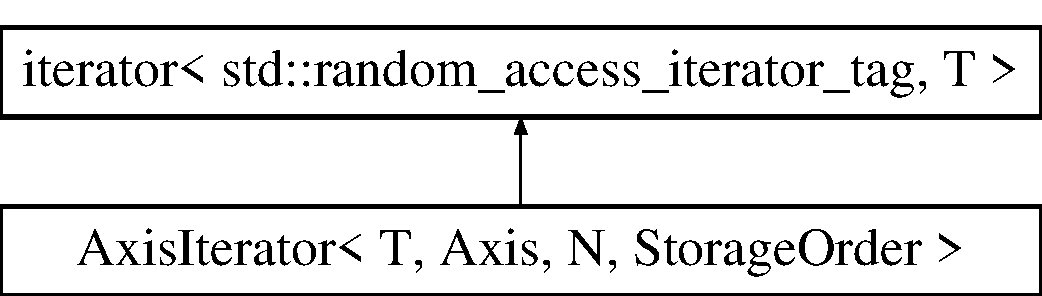
\includegraphics[height=2.000000cm]{class_d_o_1_1_axis_iterator}
\end{center}
\end{figure}
\subsection*{Public Types}
\begin{DoxyCompactItemize}
\item 
\hypertarget{class_d_o_1_1_axis_iterator_a758d02a5183e542558cd2f7ad65c683c}{typedef Base\-::value\-\_\-type {\bfseries value\-\_\-type}}\label{class_d_o_1_1_axis_iterator_a758d02a5183e542558cd2f7ad65c683c}

\item 
\hypertarget{class_d_o_1_1_axis_iterator_aa4336e7fd692b20bda7b7227fa9c9f55}{typedef Base\-::difference\-\_\-type {\bfseries difference\-\_\-type}}\label{class_d_o_1_1_axis_iterator_aa4336e7fd692b20bda7b7227fa9c9f55}

\item 
\hypertarget{class_d_o_1_1_axis_iterator_aa2158dc2d25210ef557a40d3b8a521e3}{typedef Base\-::pointer {\bfseries pointer}}\label{class_d_o_1_1_axis_iterator_aa2158dc2d25210ef557a40d3b8a521e3}

\item 
\hypertarget{class_d_o_1_1_axis_iterator_abaed3f9c23f38a6baedf841296fa931c}{typedef Base\-::reference {\bfseries reference}}\label{class_d_o_1_1_axis_iterator_abaed3f9c23f38a6baedf841296fa931c}

\item 
\hypertarget{class_d_o_1_1_axis_iterator_a61a96ce54a0b0407ce9bdd9d3f0e3934}{typedef Base\-::iterator\-\_\-category {\bfseries iterator\-\_\-category}}\label{class_d_o_1_1_axis_iterator_a61a96ce54a0b0407ce9bdd9d3f0e3934}

\item 
\hypertarget{class_d_o_1_1_axis_iterator_a94654f697ba0037a85b8a976f648c3fd}{typedef \hyperlink{class_d_o_1_1_axis_iterator}{Axis\-Iterator} {\bfseries self\-\_\-type}}\label{class_d_o_1_1_axis_iterator_a94654f697ba0037a85b8a976f648c3fd}

\item 
\hypertarget{class_d_o_1_1_axis_iterator_ae4fb477425bbeb20329d300396ac2582}{typedef Matrix$<$ int, N, 1 $>$ {\bfseries coord\-\_\-type}}\label{class_d_o_1_1_axis_iterator_ae4fb477425bbeb20329d300396ac2582}

\item 
\hypertarget{class_d_o_1_1_axis_iterator_aacf98e49e90f9aeead0ff8885fae3ac7}{typedef Matrix$<$ int, N, 1 $>$ {\bfseries vector\-\_\-type}}\label{class_d_o_1_1_axis_iterator_aacf98e49e90f9aeead0ff8885fae3ac7}

\item 
\hypertarget{class_d_o_1_1_axis_iterator_ae3ee468a9ca692fbed522f9eb22a1bd8}{typedef coord\-\_\-type \& {\bfseries coord\-\_\-reference}}\label{class_d_o_1_1_axis_iterator_ae3ee468a9ca692fbed522f9eb22a1bd8}

\item 
\hypertarget{class_d_o_1_1_axis_iterator_aa7d96038ae86b2607b1c75e8d8ff4797}{typedef pointer \& {\bfseries pointer\-\_\-reference}}\label{class_d_o_1_1_axis_iterator_aa7d96038ae86b2607b1c75e8d8ff4797}

\end{DoxyCompactItemize}
\subsection*{Public Member Functions}
\begin{DoxyCompactItemize}
\item 
\hypertarget{class_d_o_1_1_axis_iterator_abfc20ae4f3e395a95f0aeb868272fc45}{\hyperlink{class_d_o_1_1_axis_iterator_abfc20ae4f3e395a95f0aeb868272fc45}{Axis\-Iterator} (pointer\-\_\-reference pos, coord\-\_\-reference coords, const vector\-\_\-type \&strides, const vector\-\_\-type \&\hyperlink{class_d_o_1_1_axis_iterator_ab8e4e3e2a7bf18888b71bdf9dda0770b}{size})}\label{class_d_o_1_1_axis_iterator_abfc20ae4f3e395a95f0aeb868272fc45}

\begin{DoxyCompactList}\small\item\em Constructor. \end{DoxyCompactList}\item 
\hypertarget{class_d_o_1_1_axis_iterator_a94cc353f1334b1d367d4df72ceb61071}{\hyperlink{class_d_o_1_1_axis_iterator_a94cc353f1334b1d367d4df72ceb61071}{Axis\-Iterator} (const \hyperlink{class_d_o_1_1_axis_iterator}{self\-\_\-type} \&it)}\label{class_d_o_1_1_axis_iterator_a94cc353f1334b1d367d4df72ceb61071}

\begin{DoxyCompactList}\small\item\em Copy constructor. \end{DoxyCompactList}\item 
\hypertarget{class_d_o_1_1_axis_iterator_aa149c2249879e7727f33688b76bf2c99}{reference \hyperlink{class_d_o_1_1_axis_iterator_aa149c2249879e7727f33688b76bf2c99}{operator$\ast$} () const }\label{class_d_o_1_1_axis_iterator_aa149c2249879e7727f33688b76bf2c99}

\begin{DoxyCompactList}\small\item\em Referencing operator. \end{DoxyCompactList}\item 
\hypertarget{class_d_o_1_1_axis_iterator_a32d919fd1ac974efa89582486e7752de}{reference \hyperlink{class_d_o_1_1_axis_iterator_a32d919fd1ac974efa89582486e7752de}{operator\mbox{[}$\,$\mbox{]}} (int n) const }\label{class_d_o_1_1_axis_iterator_a32d919fd1ac974efa89582486e7752de}

\begin{DoxyCompactList}\small\item\em Referencing operator. \end{DoxyCompactList}\item 
\hypertarget{class_d_o_1_1_axis_iterator_a33ce448509e9cc0d73861e4c1919c7a7}{pointer \hyperlink{class_d_o_1_1_axis_iterator_a33ce448509e9cc0d73861e4c1919c7a7}{operator-\/$>$} () const }\label{class_d_o_1_1_axis_iterator_a33ce448509e9cc0d73861e4c1919c7a7}

\begin{DoxyCompactList}\small\item\em Non-\/mutable pointer operator. \end{DoxyCompactList}\item 
\hypertarget{class_d_o_1_1_axis_iterator_a74e10c48af258faf471b5ff616c6395a}{{\footnotesize template$<$typename Iterator $>$ }\\bool \hyperlink{class_d_o_1_1_axis_iterator_a74e10c48af258faf471b5ff616c6395a}{operator==} (const Iterator \&rhs) const }\label{class_d_o_1_1_axis_iterator_a74e10c48af258faf471b5ff616c6395a}

\begin{DoxyCompactList}\small\item\em Equality operator. \end{DoxyCompactList}\item 
\hypertarget{class_d_o_1_1_axis_iterator_ad3e7caef9082dd2b3f65ea3867336476}{bool \hyperlink{class_d_o_1_1_axis_iterator_ad3e7caef9082dd2b3f65ea3867336476}{operator==} (pointer pos) const }\label{class_d_o_1_1_axis_iterator_ad3e7caef9082dd2b3f65ea3867336476}

\begin{DoxyCompactList}\small\item\em Equality operator. \end{DoxyCompactList}\item 
\hypertarget{class_d_o_1_1_axis_iterator_a46311058c789c83df9d72020c4334da7}{{\footnotesize template$<$typename Iterator $>$ }\\bool \hyperlink{class_d_o_1_1_axis_iterator_a46311058c789c83df9d72020c4334da7}{operator!=} (const Iterator \&rhs) const }\label{class_d_o_1_1_axis_iterator_a46311058c789c83df9d72020c4334da7}

\begin{DoxyCompactList}\small\item\em Inequality operator. \end{DoxyCompactList}\item 
\hypertarget{class_d_o_1_1_axis_iterator_ac966afbaec9c16d1cc1bb6819810ab10}{bool \hyperlink{class_d_o_1_1_axis_iterator_ac966afbaec9c16d1cc1bb6819810ab10}{operator!=} (pointer pos) const }\label{class_d_o_1_1_axis_iterator_ac966afbaec9c16d1cc1bb6819810ab10}

\begin{DoxyCompactList}\small\item\em Inequality operator. \end{DoxyCompactList}\item 
\hypertarget{class_d_o_1_1_axis_iterator_a68c6d6abdde9fef27d6a4f2904212559}{\hyperlink{class_d_o_1_1_axis_iterator}{self\-\_\-type} \& \hyperlink{class_d_o_1_1_axis_iterator_a68c6d6abdde9fef27d6a4f2904212559}{operator++} ()}\label{class_d_o_1_1_axis_iterator_a68c6d6abdde9fef27d6a4f2904212559}

\begin{DoxyCompactList}\small\item\em Prefix increment operator. \end{DoxyCompactList}\item 
\hypertarget{class_d_o_1_1_axis_iterator_a2fa8797c1ff9e6c2ac6f879a53f60601}{\hyperlink{class_d_o_1_1_axis_iterator}{self\-\_\-type} \& \hyperlink{class_d_o_1_1_axis_iterator_a2fa8797c1ff9e6c2ac6f879a53f60601}{operator-\/-\/} ()}\label{class_d_o_1_1_axis_iterator_a2fa8797c1ff9e6c2ac6f879a53f60601}

\begin{DoxyCompactList}\small\item\em Prefix decrement operator. \end{DoxyCompactList}\item 
\hypertarget{class_d_o_1_1_axis_iterator_a39f7c37604fd9845ff487b36b6f88602}{\hyperlink{class_d_o_1_1_axis_iterator}{self\-\_\-type} \hyperlink{class_d_o_1_1_axis_iterator_a39f7c37604fd9845ff487b36b6f88602}{operator++} (int)}\label{class_d_o_1_1_axis_iterator_a39f7c37604fd9845ff487b36b6f88602}

\begin{DoxyCompactList}\small\item\em Postfix increment operator. \end{DoxyCompactList}\item 
\hypertarget{class_d_o_1_1_axis_iterator_ac8142815f977b8411faf27f7b8d804b3}{\hyperlink{class_d_o_1_1_axis_iterator}{self\-\_\-type} \hyperlink{class_d_o_1_1_axis_iterator_ac8142815f977b8411faf27f7b8d804b3}{operator-\/-\/} (int)}\label{class_d_o_1_1_axis_iterator_ac8142815f977b8411faf27f7b8d804b3}

\begin{DoxyCompactList}\small\item\em Postfix decrement operator. \end{DoxyCompactList}\item 
\hypertarget{class_d_o_1_1_axis_iterator_a2930986847b626523fbc0748b586fcdb}{\hyperlink{class_d_o_1_1_axis_iterator}{self\-\_\-type} \& \hyperlink{class_d_o_1_1_axis_iterator_a2930986847b626523fbc0748b586fcdb}{operator+=} (int n)}\label{class_d_o_1_1_axis_iterator_a2930986847b626523fbc0748b586fcdb}

\begin{DoxyCompactList}\small\item\em Arithmetic operator. \end{DoxyCompactList}\item 
\hypertarget{class_d_o_1_1_axis_iterator_a742e3ed31b69f8f5dcf0b681f638b24b}{\hyperlink{class_d_o_1_1_axis_iterator}{self\-\_\-type} \& \hyperlink{class_d_o_1_1_axis_iterator_a742e3ed31b69f8f5dcf0b681f638b24b}{operator-\/=} (int n)}\label{class_d_o_1_1_axis_iterator_a742e3ed31b69f8f5dcf0b681f638b24b}

\begin{DoxyCompactList}\small\item\em Arithmetic operator. \end{DoxyCompactList}\item 
\hypertarget{class_d_o_1_1_axis_iterator_ab8e4e3e2a7bf18888b71bdf9dda0770b}{int \hyperlink{class_d_o_1_1_axis_iterator_ab8e4e3e2a7bf18888b71bdf9dda0770b}{size} () const }\label{class_d_o_1_1_axis_iterator_ab8e4e3e2a7bf18888b71bdf9dda0770b}

\begin{DoxyCompactList}\small\item\em Constant size accessor. \end{DoxyCompactList}\end{DoxyCompactItemize}


\subsection{Detailed Description}
\subsubsection*{template$<$typename T, int Axis, int N, int Storage\-Order$>$class D\-O\-::\-Axis\-Iterator$<$ T, Axis, N, Storage\-Order $>$}

Axis iterator class for N-\/dimensional arrays. 

The documentation for this class was generated from the following file\-:\begin{DoxyCompactItemize}
\item 
src/\-D\-O/\-Core/\hyperlink{_locator_8hpp}{Locator.\-hpp}\end{DoxyCompactItemize}

\hypertarget{struct_d_o_1_1_b}{\section{B Struct Reference}
\label{struct_d_o_1_1_b}\index{B@{B}}
}


Blue channel name (R\-G\-B, R\-G\-B\-A).  




{\ttfamily \#include $<$Color.\-hpp$>$}



\subsection{Detailed Description}
Blue channel name (R\-G\-B, R\-G\-B\-A). 

The documentation for this struct was generated from the following file\-:\begin{DoxyCompactItemize}
\item 
src/\-D\-O/\-Core/\hyperlink{_color_8hpp}{Color.\-hpp}\end{DoxyCompactItemize}

\hypertarget{struct_d_o_1_1_c}{\section{C Struct Reference}
\label{struct_d_o_1_1_c}\index{C@{C}}
}


Cyan channel name (C\-M\-Y\-K).  




{\ttfamily \#include $<$Color.\-hpp$>$}



\subsection{Detailed Description}
Cyan channel name (C\-M\-Y\-K). 

The documentation for this struct was generated from the following file\-:\begin{DoxyCompactItemize}
\item 
src/\-D\-O/\-Core/\hyperlink{_color_8hpp}{Color.\-hpp}\end{DoxyCompactItemize}

\hypertarget{struct_d_o_1_1_channel_traits}{\section{Channel\-Traits$<$ T $>$ Struct Template Reference}
\label{struct_d_o_1_1_channel_traits}\index{Channel\-Traits$<$ T $>$@{Channel\-Traits$<$ T $>$}}
}


Channel traits class.  




{\ttfamily \#include $<$Color.\-hpp$>$}

\subsection*{Public Types}
\begin{DoxyCompactItemize}
\item 
\hypertarget{struct_d_o_1_1_channel_traits_a90d968700fb94b368f5a5d1bc31f38e2}{typedef T \hyperlink{struct_d_o_1_1_channel_traits_a90d968700fb94b368f5a5d1bc31f38e2}{Channel}}\label{struct_d_o_1_1_channel_traits_a90d968700fb94b368f5a5d1bc31f38e2}

\begin{DoxyCompactList}\small\item\em Channel type. \end{DoxyCompactList}\end{DoxyCompactItemize}
\subsection*{Static Public Member Functions}
\begin{DoxyCompactItemize}
\item 
\hypertarget{struct_d_o_1_1_channel_traits_a526b7ad5d0ce589d3086127cb78ffcea}{static const T \hyperlink{struct_d_o_1_1_channel_traits_a526b7ad5d0ce589d3086127cb78ffcea}{min} ()}\label{struct_d_o_1_1_channel_traits_a526b7ad5d0ce589d3086127cb78ffcea}

\begin{DoxyCompactList}\small\item\em Returns the minimum value for a specific channel type. \end{DoxyCompactList}\item 
\hypertarget{struct_d_o_1_1_channel_traits_aef359c66c9f23cc979387e202180ddd6}{static const T \hyperlink{struct_d_o_1_1_channel_traits_aef359c66c9f23cc979387e202180ddd6}{max} ()}\label{struct_d_o_1_1_channel_traits_aef359c66c9f23cc979387e202180ddd6}

\begin{DoxyCompactList}\small\item\em Returns the maximum value for a specific channel type. \end{DoxyCompactList}\item 
\hypertarget{struct_d_o_1_1_channel_traits_a746c4925f2b1d481e2059738c7ce1c3f}{static const double \hyperlink{struct_d_o_1_1_channel_traits_a746c4925f2b1d481e2059738c7ce1c3f}{double\-Min} ()}\label{struct_d_o_1_1_channel_traits_a746c4925f2b1d481e2059738c7ce1c3f}

\begin{DoxyCompactList}\small\item\em Returns the minimum value for a specific channel type (in double type). \end{DoxyCompactList}\item 
\hypertarget{struct_d_o_1_1_channel_traits_ac72bdccc104a3cd4dae1c283f06bfc99}{static const double \hyperlink{struct_d_o_1_1_channel_traits_ac72bdccc104a3cd4dae1c283f06bfc99}{double\-Max} ()}\label{struct_d_o_1_1_channel_traits_ac72bdccc104a3cd4dae1c283f06bfc99}

\begin{DoxyCompactList}\small\item\em Returns the maximum value for a specific channel type (in double type). \end{DoxyCompactList}\item 
\hypertarget{struct_d_o_1_1_channel_traits_a2e1d5319c1eafe0514be16e626e266cf}{static const double \hyperlink{struct_d_o_1_1_channel_traits_a2e1d5319c1eafe0514be16e626e266cf}{double\-Range} ()}\label{struct_d_o_1_1_channel_traits_a2e1d5319c1eafe0514be16e626e266cf}

\begin{DoxyCompactList}\small\item\em Returns the maximum range for a specific channel type (in double type). \end{DoxyCompactList}\item 
\hypertarget{struct_d_o_1_1_channel_traits_ad0d4458b14e8213cd30ca819fe69d7ed}{{\footnotesize template$<$typename U $>$ }\\static \hyperlink{struct_d_o_1_1_u}{U} \hyperlink{struct_d_o_1_1_channel_traits_ad0d4458b14e8213cd30ca819fe69d7ed}{cast} (const T \&channel)}\label{struct_d_o_1_1_channel_traits_ad0d4458b14e8213cd30ca819fe69d7ed}

\begin{DoxyCompactList}\small\item\em Cast function. \end{DoxyCompactList}\end{DoxyCompactItemize}


\subsection{Detailed Description}
\subsubsection*{template$<$typename T$>$struct D\-O\-::\-Channel\-Traits$<$ T $>$}

Channel traits class. 

This is primarily intended for color conversion and color rescaling. 

The documentation for this struct was generated from the following file\-:\begin{DoxyCompactItemize}
\item 
src/\-D\-O/\-Core/\hyperlink{_color_8hpp}{Color.\-hpp}\end{DoxyCompactItemize}

\hypertarget{struct_d_o_1_1_meta_1_1_choose}{\section{Choose$<$ flag, Is\-True, Is\-False $>$ Struct Template Reference}
\label{struct_d_o_1_1_meta_1_1_choose}\index{Choose$<$ flag, Is\-True, Is\-False $>$@{Choose$<$ flag, Is\-True, Is\-False $>$}}
}


\hyperlink{struct_d_o_1_1_meta_1_1_choose}{Choose} function.  




{\ttfamily \#include $<$Meta.\-hpp$>$}



\subsection{Detailed Description}
\subsubsection*{template$<$bool flag, typename Is\-True, typename Is\-False$>$struct D\-O\-::\-Meta\-::\-Choose$<$ flag, Is\-True, Is\-False $>$}

\hyperlink{struct_d_o_1_1_meta_1_1_choose}{Choose} function. 

The documentation for this struct was generated from the following file\-:\begin{DoxyCompactItemize}
\item 
src/\-D\-O/\-Core/\hyperlink{_meta_8hpp}{Meta.\-hpp}\end{DoxyCompactItemize}

\hypertarget{struct_d_o_1_1_meta_1_1_choose_3_01false_00_01_is_true_00_01_is_false_01_4}{\section{Choose$<$ false, Is\-True, Is\-False $>$ Struct Template Reference}
\label{struct_d_o_1_1_meta_1_1_choose_3_01false_00_01_is_true_00_01_is_false_01_4}\index{Choose$<$ false, Is\-True, Is\-False $>$@{Choose$<$ false, Is\-True, Is\-False $>$}}
}


Specialized choose function when flag is 'false'.  




{\ttfamily \#include $<$Meta.\-hpp$>$}

\subsection*{Public Types}
\begin{DoxyCompactItemize}
\item 
typedef Is\-False \hyperlink{struct_d_o_1_1_meta_1_1_choose_3_01false_00_01_is_true_00_01_is_false_01_4_a9ee7a1ba5a50997b3354cdd0a79774aa}{Type}
\end{DoxyCompactItemize}


\subsection{Detailed Description}
\subsubsection*{template$<$typename Is\-True, typename Is\-False$>$struct D\-O\-::\-Meta\-::\-Choose$<$ false, Is\-True, Is\-False $>$}

Specialized choose function when flag is 'false'. 

\subsection{Member Typedef Documentation}
\hypertarget{struct_d_o_1_1_meta_1_1_choose_3_01false_00_01_is_true_00_01_is_false_01_4_a9ee7a1ba5a50997b3354cdd0a79774aa}{\index{D\-O\-::\-Meta\-::\-Choose$<$ false, Is\-True, Is\-False $>$@{D\-O\-::\-Meta\-::\-Choose$<$ false, Is\-True, Is\-False $>$}!Type@{Type}}
\index{Type@{Type}!DO::Meta::Choose< false, IsTrue, IsFalse >@{D\-O\-::\-Meta\-::\-Choose$<$ false, Is\-True, Is\-False $>$}}
\subsubsection[{Type}]{\setlength{\rightskip}{0pt plus 5cm}typedef Is\-False {\bf Type}}}\label{struct_d_o_1_1_meta_1_1_choose_3_01false_00_01_is_true_00_01_is_false_01_4_a9ee7a1ba5a50997b3354cdd0a79774aa}
Return type. 

The documentation for this struct was generated from the following file\-:\begin{DoxyCompactItemize}
\item 
src/\-D\-O/\-Core/\hyperlink{_meta_8hpp}{Meta.\-hpp}\end{DoxyCompactItemize}

\hypertarget{struct_d_o_1_1_meta_1_1_choose_3_01true_00_01_is_true_00_01_is_false_01_4}{\section{Choose$<$ true, Is\-True, Is\-False $>$ Struct Template Reference}
\label{struct_d_o_1_1_meta_1_1_choose_3_01true_00_01_is_true_00_01_is_false_01_4}\index{Choose$<$ true, Is\-True, Is\-False $>$@{Choose$<$ true, Is\-True, Is\-False $>$}}
}


Specialized choose function when flag is 'true'.  




{\ttfamily \#include $<$Meta.\-hpp$>$}

\subsection*{Public Types}
\begin{DoxyCompactItemize}
\item 
typedef Is\-True \hyperlink{struct_d_o_1_1_meta_1_1_choose_3_01true_00_01_is_true_00_01_is_false_01_4_ab020b2d70649b728f2bab8fc98ba4cd9}{Type}
\end{DoxyCompactItemize}


\subsection{Detailed Description}
\subsubsection*{template$<$typename Is\-True, typename Is\-False$>$struct D\-O\-::\-Meta\-::\-Choose$<$ true, Is\-True, Is\-False $>$}

Specialized choose function when flag is 'true'. 

\subsection{Member Typedef Documentation}
\hypertarget{struct_d_o_1_1_meta_1_1_choose_3_01true_00_01_is_true_00_01_is_false_01_4_ab020b2d70649b728f2bab8fc98ba4cd9}{\index{D\-O\-::\-Meta\-::\-Choose$<$ true, Is\-True, Is\-False $>$@{D\-O\-::\-Meta\-::\-Choose$<$ true, Is\-True, Is\-False $>$}!Type@{Type}}
\index{Type@{Type}!DO::Meta::Choose< true, IsTrue, IsFalse >@{D\-O\-::\-Meta\-::\-Choose$<$ true, Is\-True, Is\-False $>$}}
\subsubsection[{Type}]{\setlength{\rightskip}{0pt plus 5cm}typedef Is\-True {\bf Type}}}\label{struct_d_o_1_1_meta_1_1_choose_3_01true_00_01_is_true_00_01_is_false_01_4_ab020b2d70649b728f2bab8fc98ba4cd9}
Return type. 

The documentation for this struct was generated from the following file\-:\begin{DoxyCompactItemize}
\item 
src/\-D\-O/\-Core/\hyperlink{_meta_8hpp}{Meta.\-hpp}\end{DoxyCompactItemize}

\hypertarget{class_d_o_1_1_color}{\section{Color$<$ T, Layout $>$ Class Template Reference}
\label{class_d_o_1_1_color}\index{Color$<$ T, Layout $>$@{Color$<$ T, Layout $>$}}
}


Lightweight template color class with some flexibility.  




{\ttfamily \#include $<$Color.\-hpp$>$}

Inheritance diagram for Color$<$ T, Layout $>$\-:\begin{figure}[H]
\begin{center}
\leavevmode
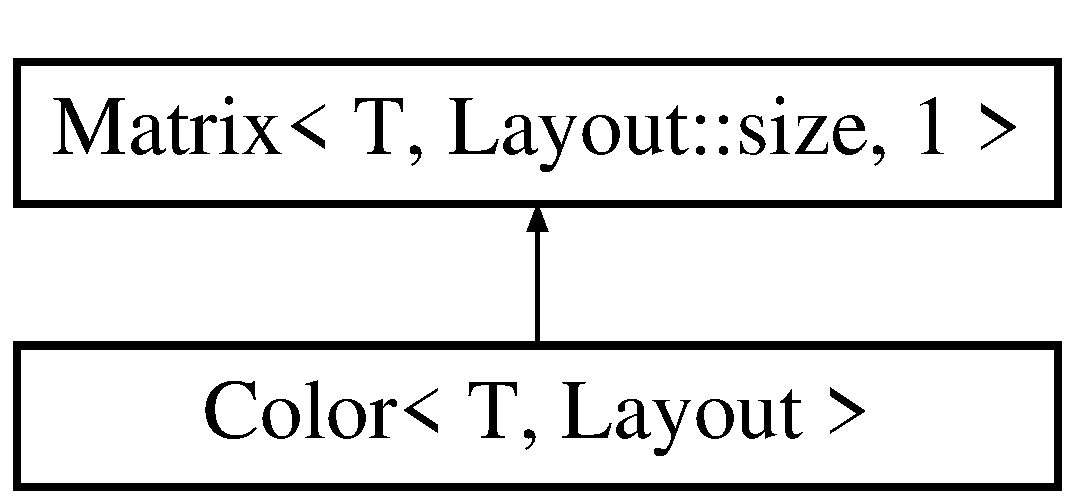
\includegraphics[height=2.000000cm]{class_d_o_1_1_color}
\end{center}
\end{figure}
\subsection*{Public Types}
\begin{DoxyCompactItemize}
\item 
\hypertarget{class_d_o_1_1_color_a4fc05512d90a4b0e4d7a6ca6e56b9ed4}{typedef T \hyperlink{class_d_o_1_1_color_a4fc05512d90a4b0e4d7a6ca6e56b9ed4}{Channel\-Type}}\label{class_d_o_1_1_color_a4fc05512d90a4b0e4d7a6ca6e56b9ed4}

\begin{DoxyCompactList}\small\item\em Channel type. \end{DoxyCompactList}\item 
\hypertarget{class_d_o_1_1_color_a7a81d850ad8c8ac23245eabb7fae392b}{typedef Layout \hyperlink{class_d_o_1_1_color_a7a81d850ad8c8ac23245eabb7fae392b}{Color\-Layout}}\label{class_d_o_1_1_color_a7a81d850ad8c8ac23245eabb7fae392b}

\begin{DoxyCompactList}\small\item\em Layout type (R\-G\-B, B\-G\-R, R\-G\-B\-A, C\-M\-Y\-K, ...) \end{DoxyCompactList}\end{DoxyCompactItemize}
\subsection*{Public Member Functions}
\begin{DoxyCompactItemize}
\item 
\hypertarget{class_d_o_1_1_color_a1589b83974b42a2f3315624f14c3c92c}{\hyperlink{class_d_o_1_1_color_a1589b83974b42a2f3315624f14c3c92c}{Color} ()}\label{class_d_o_1_1_color_a1589b83974b42a2f3315624f14c3c92c}

\begin{DoxyCompactList}\small\item\em Default constructor. \end{DoxyCompactList}\item 
\hypertarget{class_d_o_1_1_color_a86b6c08f8a3c0123d9f4df11e8ffe526}{\hyperlink{class_d_o_1_1_color_a86b6c08f8a3c0123d9f4df11e8ffe526}{Color} (T x, T \hyperlink{group___channel_accessors_gac90c52c5b3a7b2a7e3761e6e84f25778}{y}, T z)}\label{class_d_o_1_1_color_a86b6c08f8a3c0123d9f4df11e8ffe526}

\begin{DoxyCompactList}\small\item\em Custom constructor. \end{DoxyCompactList}\item 
\hypertarget{class_d_o_1_1_color_abad592080ccdd941af94bfe0150012af}{\hyperlink{class_d_o_1_1_color_abad592080ccdd941af94bfe0150012af}{Color} (T x, T \hyperlink{group___channel_accessors_gac90c52c5b3a7b2a7e3761e6e84f25778}{y}, T z, T t)}\label{class_d_o_1_1_color_abad592080ccdd941af94bfe0150012af}

\begin{DoxyCompactList}\small\item\em Custom constructor. \end{DoxyCompactList}\item 
\hypertarget{class_d_o_1_1_color_a086c48494a60de214f91d716a7510e71}{\hyperlink{class_d_o_1_1_color_a086c48494a60de214f91d716a7510e71}{Color} (const Base \&x)}\label{class_d_o_1_1_color_a086c48494a60de214f91d716a7510e71}

\begin{DoxyCompactList}\small\item\em Copy constructor. \end{DoxyCompactList}\item 
\hypertarget{class_d_o_1_1_color_acd86e5a133b3e760a79309ffff2bc996}{{\footnotesize template$<$typename Other\-Derived $>$ }\\\hyperlink{class_d_o_1_1_color}{Color} \& \hyperlink{class_d_o_1_1_color_acd86e5a133b3e760a79309ffff2bc996}{operator=} (const Eigen\-::\-Matrix\-Base$<$ Other\-Derived $>$ \&other)}\label{class_d_o_1_1_color_acd86e5a133b3e760a79309ffff2bc996}

\begin{DoxyCompactList}\small\item\em Assignment operator. \end{DoxyCompactList}\item 
\hypertarget{class_d_o_1_1_color_af4923830e61e808a81501dc9344bc731}{{\footnotesize template$<$typename Channel $>$ }\\const T \& \hyperlink{class_d_o_1_1_color_af4923830e61e808a81501dc9344bc731}{channel} () const }\label{class_d_o_1_1_color_af4923830e61e808a81501dc9344bc731}

\begin{DoxyCompactList}\small\item\em Constant channel accessor. \end{DoxyCompactList}\item 
\hypertarget{class_d_o_1_1_color_a0b6849e95fe39fc5321a33ca630fd5df}{{\footnotesize template$<$typename Channel $>$ }\\\hyperlink{class_d_o_1_1_color_a4fc05512d90a4b0e4d7a6ca6e56b9ed4}{Channel\-Type} \& \hyperlink{class_d_o_1_1_color_a0b6849e95fe39fc5321a33ca630fd5df}{channel} ()}\label{class_d_o_1_1_color_a0b6849e95fe39fc5321a33ca630fd5df}

\begin{DoxyCompactList}\small\item\em Mutable channel accessor. \end{DoxyCompactList}\item 
\hypertarget{class_d_o_1_1_color_aa025989b00244ede2f541d9c79a36724}{int \hyperlink{class_d_o_1_1_color_aa025989b00244ede2f541d9c79a36724}{num\-Channels} () const }\label{class_d_o_1_1_color_aa025989b00244ede2f541d9c79a36724}

\begin{DoxyCompactList}\small\item\em Returns the number of channels. \end{DoxyCompactList}\end{DoxyCompactItemize}


\subsection{Detailed Description}
\subsubsection*{template$<$typename T, typename Layout = Rgb$>$class D\-O\-::\-Color$<$ T, Layout $>$}

Lightweight template color class with some flexibility. 

The color space and layout can have some flexibility. Here are some supported color space and layout examples\-: R\-G\-B, B\-G\-R, R\-G\-B\-A, B\-G\-R\-A, A\-R\-G\-B, Y\-U\-V, H\-S\-V.

However every channel {\itshape must} have the same bit depth. For complex packed pixels with complex color layouts, consider Boost.\-G\-I\-L instead.

Also note this may not be intended for video processing!

Anyways, I wanted to do some image processing as conveniently as possible because\-:
\begin{DoxyItemize}
\item I want to avoid introducing a dependency with Boost in the Core module because it is too big...
\item I had a bad user experience with the A\-P\-I of Boost.\-G\-I\-L. It seems neither easy to remember nor easy to use and I wasted a lot of time with the documentation. 
\end{DoxyItemize}

The documentation for this class was generated from the following file\-:\begin{DoxyCompactItemize}
\item 
src/\-D\-O/\-Core/\hyperlink{_color_8hpp}{Color.\-hpp}\end{DoxyCompactItemize}

\hypertarget{struct_d_o_1_1_color_traits}{\section{Color\-Traits$<$ Color\-\_\- $>$ Struct Template Reference}
\label{struct_d_o_1_1_color_traits}\index{Color\-Traits$<$ Color\-\_\- $>$@{Color\-Traits$<$ Color\-\_\- $>$}}
}


\hyperlink{class_d_o_1_1_color}{Color} traits class.  




{\ttfamily \#include $<$Color.\-hpp$>$}

\subsection*{Public Types}
\begin{DoxyCompactItemize}
\item 
enum \{ {\bfseries Num\-Channels} = Color\-\_\-\-:\-:Rows\-At\-Compile\-Time
 \}
\begin{DoxyCompactList}\small\item\em Number of channels. \end{DoxyCompactList}\item 
\hypertarget{struct_d_o_1_1_color_traits_a8d45fa3ac7947ce1caba83d2bad66677}{typedef Color\-\_\- \hyperlink{struct_d_o_1_1_color_traits_a8d45fa3ac7947ce1caba83d2bad66677}{Color}}\label{struct_d_o_1_1_color_traits_a8d45fa3ac7947ce1caba83d2bad66677}

\begin{DoxyCompactList}\small\item\em \hyperlink{class_d_o_1_1_color}{Color} type. \end{DoxyCompactList}\item 
\hypertarget{struct_d_o_1_1_color_traits_ad14c104c9edbe1cd9020ea82f3cdb0f5}{typedef Color\-\_\-\-::\-Channel\-Type \hyperlink{struct_d_o_1_1_color_traits_ad14c104c9edbe1cd9020ea82f3cdb0f5}{Channel\-Type}}\label{struct_d_o_1_1_color_traits_ad14c104c9edbe1cd9020ea82f3cdb0f5}

\begin{DoxyCompactList}\small\item\em Channel type. \end{DoxyCompactList}\item 
\hypertarget{struct_d_o_1_1_color_traits_a1936ea193f7f09f57144dd97e0fd7969}{typedef Color\-\_\-\-::\-Color\-Layout \hyperlink{struct_d_o_1_1_color_traits_a1936ea193f7f09f57144dd97e0fd7969}{Color\-Layout}}\label{struct_d_o_1_1_color_traits_a1936ea193f7f09f57144dd97e0fd7969}

\begin{DoxyCompactList}\small\item\em \hyperlink{class_d_o_1_1_color}{Color} layout type. \end{DoxyCompactList}\item 
\hypertarget{struct_d_o_1_1_color_traits_acb6a3ad1b3c0fd4f07d65dfc4fb89623}{typedef \hyperlink{class_d_o_1_1_color}{D\-O\-::\-Color}$<$ double, \\*
\hyperlink{struct_d_o_1_1_color_traits_a1936ea193f7f09f57144dd97e0fd7969}{Color\-Layout} $>$ \hyperlink{struct_d_o_1_1_color_traits_acb6a3ad1b3c0fd4f07d65dfc4fb89623}{Color64f}}\label{struct_d_o_1_1_color_traits_acb6a3ad1b3c0fd4f07d65dfc4fb89623}

\begin{DoxyCompactList}\small\item\em \hyperlink{class_d_o_1_1_color}{Color} type where the channel type is 'double'. \end{DoxyCompactList}\end{DoxyCompactItemize}
\subsection*{Static Public Member Functions}
\begin{DoxyCompactItemize}
\item 
\hypertarget{struct_d_o_1_1_color_traits_aef35bf35a1f3fbe0fb53bde998f12937}{static const \hyperlink{struct_d_o_1_1_color_traits_a8d45fa3ac7947ce1caba83d2bad66677}{Color} \hyperlink{struct_d_o_1_1_color_traits_aef35bf35a1f3fbe0fb53bde998f12937}{zero} ()}\label{struct_d_o_1_1_color_traits_aef35bf35a1f3fbe0fb53bde998f12937}

\begin{DoxyCompactList}\small\item\em Zero color (=Black for R\-G\-B). \end{DoxyCompactList}\item 
\hypertarget{struct_d_o_1_1_color_traits_a78baae966b690cee8810329019841a65}{static const \hyperlink{struct_d_o_1_1_color_traits_a8d45fa3ac7947ce1caba83d2bad66677}{Color} \hyperlink{struct_d_o_1_1_color_traits_a78baae966b690cee8810329019841a65}{min} ()}\label{struct_d_o_1_1_color_traits_a78baae966b690cee8810329019841a65}

\begin{DoxyCompactList}\small\item\em Entry-\/wise minimum color (=Black for R\-G\-B). \end{DoxyCompactList}\item 
\hypertarget{struct_d_o_1_1_color_traits_a363300396ad213712625fdc984648f2e}{static const \hyperlink{struct_d_o_1_1_color_traits_a8d45fa3ac7947ce1caba83d2bad66677}{Color} \hyperlink{struct_d_o_1_1_color_traits_a363300396ad213712625fdc984648f2e}{max} ()}\label{struct_d_o_1_1_color_traits_a363300396ad213712625fdc984648f2e}

\begin{DoxyCompactList}\small\item\em Entry-\/wise maximum color (=White for R\-G\-B). \end{DoxyCompactList}\item 
\hypertarget{struct_d_o_1_1_color_traits_a2842b58e25ca3ad8048353e30362e784}{static Matrix$<$ double, \\*
Num\-Channels, 1 $>$ \hyperlink{struct_d_o_1_1_color_traits_a2842b58e25ca3ad8048353e30362e784}{double\-Min} ()}\label{struct_d_o_1_1_color_traits_a2842b58e25ca3ad8048353e30362e784}

\begin{DoxyCompactList}\small\item\em Entry-\/wise minimum color (=Black for R\-G\-B). \end{DoxyCompactList}\item 
\hypertarget{struct_d_o_1_1_color_traits_a41190a80640221fab7f3b6de0f2cc8dc}{static Matrix$<$ double, \\*
Num\-Channels, 1 $>$ \hyperlink{struct_d_o_1_1_color_traits_a41190a80640221fab7f3b6de0f2cc8dc}{double\-Max} ()}\label{struct_d_o_1_1_color_traits_a41190a80640221fab7f3b6de0f2cc8dc}

\begin{DoxyCompactList}\small\item\em Entry-\/wise maximum color (=White for R\-G\-B). \end{DoxyCompactList}\item 
\hypertarget{struct_d_o_1_1_color_traits_abbd492ef4826701b8b1a1e523cdc2a69}{static Matrix$<$ double, \\*
Num\-Channels, 1 $>$ \hyperlink{struct_d_o_1_1_color_traits_abbd492ef4826701b8b1a1e523cdc2a69}{double\-Range} ()}\label{struct_d_o_1_1_color_traits_abbd492ef4826701b8b1a1e523cdc2a69}

\begin{DoxyCompactList}\small\item\em Entry-\/wise range. \end{DoxyCompactList}\end{DoxyCompactItemize}


\subsection{Detailed Description}
\subsubsection*{template$<$typename Color\-\_\-$>$struct D\-O\-::\-Color\-Traits$<$ Color\-\_\- $>$}

\hyperlink{class_d_o_1_1_color}{Color} traits class. 

It is essentially intended for color conversion and image rescaling in order to view images. 

The documentation for this struct was generated from the following file\-:\begin{DoxyCompactItemize}
\item 
src/\-D\-O/\-Core/\hyperlink{_color_8hpp}{Color.\-hpp}\end{DoxyCompactItemize}

\hypertarget{struct_d_o_1_1_color_traits_3_01char_01_4}{\section{Color\-Traits$<$ char $>$ Struct Template Reference}
\label{struct_d_o_1_1_color_traits_3_01char_01_4}\index{Color\-Traits$<$ char $>$@{Color\-Traits$<$ char $>$}}
}


Specialized color traits class for 'char' grayscale color.  




{\ttfamily \#include $<$Color.\-hpp$>$}

\subsection*{Public Types}
\begin{DoxyCompactItemize}
\item 
enum \{ {\bfseries Num\-Channels} = 1
 \}
\item 
typedef char \hyperlink{struct_d_o_1_1_color_traits_3_01char_01_4_a5e11ed2b5bbfd2ec0290ba691e77315c}{Color}
\item 
typedef char \hyperlink{struct_d_o_1_1_color_traits_3_01char_01_4_a068771d43562e39b0f446c960a439e81}{Channel\-Type}
\item 
typedef double \hyperlink{struct_d_o_1_1_color_traits_3_01char_01_4_a9a301fd8ba0a7225e38351d3e5b2e4d3}{Color64f}
\item 
typedef \hyperlink{struct_d_o_1_1_gray}{Gray} \hyperlink{struct_d_o_1_1_color_traits_3_01char_01_4_a7c9d599cfa0d1404784fbe60e6bcfd24}{Color\-Layout}
\end{DoxyCompactItemize}
\subsection*{Static Public Member Functions}
\begin{DoxyCompactItemize}
\item 
static \hyperlink{struct_d_o_1_1_color_traits_3_01char_01_4_a5e11ed2b5bbfd2ec0290ba691e77315c}{Color} \hyperlink{struct_d_o_1_1_color_traits_3_01char_01_4_a57b00f8db42515f404e06ab933932125}{zero} ()
\item 
static \hyperlink{struct_d_o_1_1_color_traits_3_01char_01_4_a5e11ed2b5bbfd2ec0290ba691e77315c}{Color} \hyperlink{struct_d_o_1_1_color_traits_3_01char_01_4_a1cd81f912af766f8004e4d5a82a7128b}{min} ()
\item 
static \hyperlink{struct_d_o_1_1_color_traits_3_01char_01_4_a5e11ed2b5bbfd2ec0290ba691e77315c}{Color} \hyperlink{struct_d_o_1_1_color_traits_3_01char_01_4_aded391d5e231096e135e08760c0fbeb6}{max} ()
\item 
static double \hyperlink{struct_d_o_1_1_color_traits_3_01char_01_4_aa122aba748bfd453a27d2c30b368dbc3}{double\-Min} ()
\item 
static double \hyperlink{struct_d_o_1_1_color_traits_3_01char_01_4_ab9fb6b1bb12e23b725453a69f6193c30}{double\-Max} ()
\item 
static double \hyperlink{struct_d_o_1_1_color_traits_3_01char_01_4_aed64f95e634b8dac0ae5a0aed2b45740}{double\-Range} ()
\end{DoxyCompactItemize}


\subsection{Detailed Description}
\subsubsection*{template$<$$>$struct D\-O\-::\-Color\-Traits$<$ char $>$}

Specialized color traits class for 'char' grayscale color. 

\subsection{Member Typedef Documentation}
\hypertarget{struct_d_o_1_1_color_traits_3_01char_01_4_a068771d43562e39b0f446c960a439e81}{\index{D\-O\-::\-Color\-Traits$<$ char $>$@{D\-O\-::\-Color\-Traits$<$ char $>$}!Channel\-Type@{Channel\-Type}}
\index{Channel\-Type@{Channel\-Type}!DO::ColorTraits< char >@{D\-O\-::\-Color\-Traits$<$ char $>$}}
\subsubsection[{Channel\-Type}]{\setlength{\rightskip}{0pt plus 5cm}typedef char {\bf Channel\-Type}}}\label{struct_d_o_1_1_color_traits_3_01char_01_4_a068771d43562e39b0f446c960a439e81}
Channel type. \hypertarget{struct_d_o_1_1_color_traits_3_01char_01_4_a5e11ed2b5bbfd2ec0290ba691e77315c}{\index{D\-O\-::\-Color\-Traits$<$ char $>$@{D\-O\-::\-Color\-Traits$<$ char $>$}!Color@{Color}}
\index{Color@{Color}!DO::ColorTraits< char >@{D\-O\-::\-Color\-Traits$<$ char $>$}}
\subsubsection[{Color}]{\setlength{\rightskip}{0pt plus 5cm}typedef char {\bf Color}}}\label{struct_d_o_1_1_color_traits_3_01char_01_4_a5e11ed2b5bbfd2ec0290ba691e77315c}
\hyperlink{class_d_o_1_1_color}{Color} type. \hypertarget{struct_d_o_1_1_color_traits_3_01char_01_4_a9a301fd8ba0a7225e38351d3e5b2e4d3}{\index{D\-O\-::\-Color\-Traits$<$ char $>$@{D\-O\-::\-Color\-Traits$<$ char $>$}!Color64f@{Color64f}}
\index{Color64f@{Color64f}!DO::ColorTraits< char >@{D\-O\-::\-Color\-Traits$<$ char $>$}}
\subsubsection[{Color64f}]{\setlength{\rightskip}{0pt plus 5cm}typedef double {\bf Color64f}}}\label{struct_d_o_1_1_color_traits_3_01char_01_4_a9a301fd8ba0a7225e38351d3e5b2e4d3}
Double floating precision grayscale color type. \hypertarget{struct_d_o_1_1_color_traits_3_01char_01_4_a7c9d599cfa0d1404784fbe60e6bcfd24}{\index{D\-O\-::\-Color\-Traits$<$ char $>$@{D\-O\-::\-Color\-Traits$<$ char $>$}!Color\-Layout@{Color\-Layout}}
\index{Color\-Layout@{Color\-Layout}!DO::ColorTraits< char >@{D\-O\-::\-Color\-Traits$<$ char $>$}}
\subsubsection[{Color\-Layout}]{\setlength{\rightskip}{0pt plus 5cm}typedef {\bf Gray} {\bf Color\-Layout}}}\label{struct_d_o_1_1_color_traits_3_01char_01_4_a7c9d599cfa0d1404784fbe60e6bcfd24}
Grayscale color layout. 

\subsection{Member Enumeration Documentation}
\hypertarget{struct_d_o_1_1_color_traits_3_01char_01_4_a726ca809ffd3d67ab4b8476646f26635}{\subsubsection[{anonymous enum}]{\setlength{\rightskip}{0pt plus 5cm}anonymous enum}}\label{struct_d_o_1_1_color_traits_3_01char_01_4_a726ca809ffd3d67ab4b8476646f26635}
Number of channels. 

\subsection{Member Function Documentation}
\hypertarget{struct_d_o_1_1_color_traits_3_01char_01_4_ab9fb6b1bb12e23b725453a69f6193c30}{\index{D\-O\-::\-Color\-Traits$<$ char $>$@{D\-O\-::\-Color\-Traits$<$ char $>$}!double\-Max@{double\-Max}}
\index{double\-Max@{double\-Max}!DO::ColorTraits< char >@{D\-O\-::\-Color\-Traits$<$ char $>$}}
\subsubsection[{double\-Max}]{\setlength{\rightskip}{0pt plus 5cm}static double double\-Max (
\begin{DoxyParamCaption}
{}
\end{DoxyParamCaption}
)\hspace{0.3cm}{\ttfamily [inline]}, {\ttfamily [static]}}}\label{struct_d_o_1_1_color_traits_3_01char_01_4_ab9fb6b1bb12e23b725453a69f6193c30}
Double maximum grayscale value (=White). \hypertarget{struct_d_o_1_1_color_traits_3_01char_01_4_aa122aba748bfd453a27d2c30b368dbc3}{\index{D\-O\-::\-Color\-Traits$<$ char $>$@{D\-O\-::\-Color\-Traits$<$ char $>$}!double\-Min@{double\-Min}}
\index{double\-Min@{double\-Min}!DO::ColorTraits< char >@{D\-O\-::\-Color\-Traits$<$ char $>$}}
\subsubsection[{double\-Min}]{\setlength{\rightskip}{0pt plus 5cm}static double double\-Min (
\begin{DoxyParamCaption}
{}
\end{DoxyParamCaption}
)\hspace{0.3cm}{\ttfamily [inline]}, {\ttfamily [static]}}}\label{struct_d_o_1_1_color_traits_3_01char_01_4_aa122aba748bfd453a27d2c30b368dbc3}
Double minimum grayscale value (=Black). \hypertarget{struct_d_o_1_1_color_traits_3_01char_01_4_aed64f95e634b8dac0ae5a0aed2b45740}{\index{D\-O\-::\-Color\-Traits$<$ char $>$@{D\-O\-::\-Color\-Traits$<$ char $>$}!double\-Range@{double\-Range}}
\index{double\-Range@{double\-Range}!DO::ColorTraits< char >@{D\-O\-::\-Color\-Traits$<$ char $>$}}
\subsubsection[{double\-Range}]{\setlength{\rightskip}{0pt plus 5cm}static double double\-Range (
\begin{DoxyParamCaption}
{}
\end{DoxyParamCaption}
)\hspace{0.3cm}{\ttfamily [inline]}, {\ttfamily [static]}}}\label{struct_d_o_1_1_color_traits_3_01char_01_4_aed64f95e634b8dac0ae5a0aed2b45740}
Double range grayscale value. \hypertarget{struct_d_o_1_1_color_traits_3_01char_01_4_aded391d5e231096e135e08760c0fbeb6}{\index{D\-O\-::\-Color\-Traits$<$ char $>$@{D\-O\-::\-Color\-Traits$<$ char $>$}!max@{max}}
\index{max@{max}!DO::ColorTraits< char >@{D\-O\-::\-Color\-Traits$<$ char $>$}}
\subsubsection[{max}]{\setlength{\rightskip}{0pt plus 5cm}static {\bf Color} max (
\begin{DoxyParamCaption}
{}
\end{DoxyParamCaption}
)\hspace{0.3cm}{\ttfamily [inline]}, {\ttfamily [static]}}}\label{struct_d_o_1_1_color_traits_3_01char_01_4_aded391d5e231096e135e08760c0fbeb6}
Maximum grayscale value (=White). \hypertarget{struct_d_o_1_1_color_traits_3_01char_01_4_a1cd81f912af766f8004e4d5a82a7128b}{\index{D\-O\-::\-Color\-Traits$<$ char $>$@{D\-O\-::\-Color\-Traits$<$ char $>$}!min@{min}}
\index{min@{min}!DO::ColorTraits< char >@{D\-O\-::\-Color\-Traits$<$ char $>$}}
\subsubsection[{min}]{\setlength{\rightskip}{0pt plus 5cm}static {\bf Color} min (
\begin{DoxyParamCaption}
{}
\end{DoxyParamCaption}
)\hspace{0.3cm}{\ttfamily [inline]}, {\ttfamily [static]}}}\label{struct_d_o_1_1_color_traits_3_01char_01_4_a1cd81f912af766f8004e4d5a82a7128b}
Minimum grayscale value (=Black). \hypertarget{struct_d_o_1_1_color_traits_3_01char_01_4_a57b00f8db42515f404e06ab933932125}{\index{D\-O\-::\-Color\-Traits$<$ char $>$@{D\-O\-::\-Color\-Traits$<$ char $>$}!zero@{zero}}
\index{zero@{zero}!DO::ColorTraits< char >@{D\-O\-::\-Color\-Traits$<$ char $>$}}
\subsubsection[{zero}]{\setlength{\rightskip}{0pt plus 5cm}static {\bf Color} zero (
\begin{DoxyParamCaption}
{}
\end{DoxyParamCaption}
)\hspace{0.3cm}{\ttfamily [inline]}, {\ttfamily [static]}}}\label{struct_d_o_1_1_color_traits_3_01char_01_4_a57b00f8db42515f404e06ab933932125}
Zero grayscale value (=Black). 

The documentation for this struct was generated from the following file\-:\begin{DoxyCompactItemize}
\item 
src/\-D\-O/\-Core/\hyperlink{_color_8hpp}{Color.\-hpp}\end{DoxyCompactItemize}

\hypertarget{struct_d_o_1_1_color_traits_3_01double_01_4}{\section{Color\-Traits$<$ double $>$ Struct Template Reference}
\label{struct_d_o_1_1_color_traits_3_01double_01_4}\index{Color\-Traits$<$ double $>$@{Color\-Traits$<$ double $>$}}
}


Specialized color traits class for 'double' grayscale color.  




{\ttfamily \#include $<$Color.\-hpp$>$}

\subsection*{Public Types}
\begin{DoxyCompactItemize}
\item 
enum \{ {\bfseries Num\-Channels} = 1
 \}
\item 
typedef double \hyperlink{struct_d_o_1_1_color_traits_3_01double_01_4_a8b96d8e5cd628393636da37219eb5a2d}{Color}
\item 
typedef double \hyperlink{struct_d_o_1_1_color_traits_3_01double_01_4_ae21d84313286d731e69913a7fd7a538e}{Channel\-Type}
\item 
typedef double \hyperlink{struct_d_o_1_1_color_traits_3_01double_01_4_a9a301fd8ba0a7225e38351d3e5b2e4d3}{Color64f}
\item 
typedef \hyperlink{struct_d_o_1_1_gray}{Gray} \hyperlink{struct_d_o_1_1_color_traits_3_01double_01_4_a7c9d599cfa0d1404784fbe60e6bcfd24}{Color\-Layout}
\end{DoxyCompactItemize}
\subsection*{Static Public Member Functions}
\begin{DoxyCompactItemize}
\item 
static \hyperlink{struct_d_o_1_1_color_traits_3_01double_01_4_a8b96d8e5cd628393636da37219eb5a2d}{Color} \hyperlink{struct_d_o_1_1_color_traits_3_01double_01_4_a57b00f8db42515f404e06ab933932125}{zero} ()
\item 
static \hyperlink{struct_d_o_1_1_color_traits_3_01double_01_4_a8b96d8e5cd628393636da37219eb5a2d}{Color} \hyperlink{struct_d_o_1_1_color_traits_3_01double_01_4_a1cd81f912af766f8004e4d5a82a7128b}{min} ()
\item 
static \hyperlink{struct_d_o_1_1_color_traits_3_01double_01_4_a8b96d8e5cd628393636da37219eb5a2d}{Color} \hyperlink{struct_d_o_1_1_color_traits_3_01double_01_4_aded391d5e231096e135e08760c0fbeb6}{max} ()
\item 
static double \hyperlink{struct_d_o_1_1_color_traits_3_01double_01_4_aa122aba748bfd453a27d2c30b368dbc3}{double\-Min} ()
\item 
static double \hyperlink{struct_d_o_1_1_color_traits_3_01double_01_4_ab9fb6b1bb12e23b725453a69f6193c30}{double\-Max} ()
\item 
static double \hyperlink{struct_d_o_1_1_color_traits_3_01double_01_4_aed64f95e634b8dac0ae5a0aed2b45740}{double\-Range} ()
\end{DoxyCompactItemize}


\subsection{Detailed Description}
\subsubsection*{template$<$$>$struct D\-O\-::\-Color\-Traits$<$ double $>$}

Specialized color traits class for 'double' grayscale color. 

\subsection{Member Typedef Documentation}
\hypertarget{struct_d_o_1_1_color_traits_3_01double_01_4_ae21d84313286d731e69913a7fd7a538e}{\index{D\-O\-::\-Color\-Traits$<$ double $>$@{D\-O\-::\-Color\-Traits$<$ double $>$}!Channel\-Type@{Channel\-Type}}
\index{Channel\-Type@{Channel\-Type}!DO::ColorTraits< double >@{D\-O\-::\-Color\-Traits$<$ double $>$}}
\subsubsection[{Channel\-Type}]{\setlength{\rightskip}{0pt plus 5cm}typedef double {\bf Channel\-Type}}}\label{struct_d_o_1_1_color_traits_3_01double_01_4_ae21d84313286d731e69913a7fd7a538e}
Channel type. \hypertarget{struct_d_o_1_1_color_traits_3_01double_01_4_a8b96d8e5cd628393636da37219eb5a2d}{\index{D\-O\-::\-Color\-Traits$<$ double $>$@{D\-O\-::\-Color\-Traits$<$ double $>$}!Color@{Color}}
\index{Color@{Color}!DO::ColorTraits< double >@{D\-O\-::\-Color\-Traits$<$ double $>$}}
\subsubsection[{Color}]{\setlength{\rightskip}{0pt plus 5cm}typedef double {\bf Color}}}\label{struct_d_o_1_1_color_traits_3_01double_01_4_a8b96d8e5cd628393636da37219eb5a2d}
\hyperlink{class_d_o_1_1_color}{Color} type. \hypertarget{struct_d_o_1_1_color_traits_3_01double_01_4_a9a301fd8ba0a7225e38351d3e5b2e4d3}{\index{D\-O\-::\-Color\-Traits$<$ double $>$@{D\-O\-::\-Color\-Traits$<$ double $>$}!Color64f@{Color64f}}
\index{Color64f@{Color64f}!DO::ColorTraits< double >@{D\-O\-::\-Color\-Traits$<$ double $>$}}
\subsubsection[{Color64f}]{\setlength{\rightskip}{0pt plus 5cm}typedef double {\bf Color64f}}}\label{struct_d_o_1_1_color_traits_3_01double_01_4_a9a301fd8ba0a7225e38351d3e5b2e4d3}
Double floating precision grayscale color type. \hypertarget{struct_d_o_1_1_color_traits_3_01double_01_4_a7c9d599cfa0d1404784fbe60e6bcfd24}{\index{D\-O\-::\-Color\-Traits$<$ double $>$@{D\-O\-::\-Color\-Traits$<$ double $>$}!Color\-Layout@{Color\-Layout}}
\index{Color\-Layout@{Color\-Layout}!DO::ColorTraits< double >@{D\-O\-::\-Color\-Traits$<$ double $>$}}
\subsubsection[{Color\-Layout}]{\setlength{\rightskip}{0pt plus 5cm}typedef {\bf Gray} {\bf Color\-Layout}}}\label{struct_d_o_1_1_color_traits_3_01double_01_4_a7c9d599cfa0d1404784fbe60e6bcfd24}
Grayscale color layout. 

\subsection{Member Enumeration Documentation}
\hypertarget{struct_d_o_1_1_color_traits_3_01double_01_4_a385c44f6fb256e5716a2302a5b940388}{\subsubsection[{anonymous enum}]{\setlength{\rightskip}{0pt plus 5cm}anonymous enum}}\label{struct_d_o_1_1_color_traits_3_01double_01_4_a385c44f6fb256e5716a2302a5b940388}
Number of channels. 

\subsection{Member Function Documentation}
\hypertarget{struct_d_o_1_1_color_traits_3_01double_01_4_ab9fb6b1bb12e23b725453a69f6193c30}{\index{D\-O\-::\-Color\-Traits$<$ double $>$@{D\-O\-::\-Color\-Traits$<$ double $>$}!double\-Max@{double\-Max}}
\index{double\-Max@{double\-Max}!DO::ColorTraits< double >@{D\-O\-::\-Color\-Traits$<$ double $>$}}
\subsubsection[{double\-Max}]{\setlength{\rightskip}{0pt plus 5cm}static double double\-Max (
\begin{DoxyParamCaption}
{}
\end{DoxyParamCaption}
)\hspace{0.3cm}{\ttfamily [inline]}, {\ttfamily [static]}}}\label{struct_d_o_1_1_color_traits_3_01double_01_4_ab9fb6b1bb12e23b725453a69f6193c30}
Double maximum grayscale value (=White). \hypertarget{struct_d_o_1_1_color_traits_3_01double_01_4_aa122aba748bfd453a27d2c30b368dbc3}{\index{D\-O\-::\-Color\-Traits$<$ double $>$@{D\-O\-::\-Color\-Traits$<$ double $>$}!double\-Min@{double\-Min}}
\index{double\-Min@{double\-Min}!DO::ColorTraits< double >@{D\-O\-::\-Color\-Traits$<$ double $>$}}
\subsubsection[{double\-Min}]{\setlength{\rightskip}{0pt plus 5cm}static double double\-Min (
\begin{DoxyParamCaption}
{}
\end{DoxyParamCaption}
)\hspace{0.3cm}{\ttfamily [inline]}, {\ttfamily [static]}}}\label{struct_d_o_1_1_color_traits_3_01double_01_4_aa122aba748bfd453a27d2c30b368dbc3}
Double minimum grayscale value (=Black). \hypertarget{struct_d_o_1_1_color_traits_3_01double_01_4_aed64f95e634b8dac0ae5a0aed2b45740}{\index{D\-O\-::\-Color\-Traits$<$ double $>$@{D\-O\-::\-Color\-Traits$<$ double $>$}!double\-Range@{double\-Range}}
\index{double\-Range@{double\-Range}!DO::ColorTraits< double >@{D\-O\-::\-Color\-Traits$<$ double $>$}}
\subsubsection[{double\-Range}]{\setlength{\rightskip}{0pt plus 5cm}static double double\-Range (
\begin{DoxyParamCaption}
{}
\end{DoxyParamCaption}
)\hspace{0.3cm}{\ttfamily [inline]}, {\ttfamily [static]}}}\label{struct_d_o_1_1_color_traits_3_01double_01_4_aed64f95e634b8dac0ae5a0aed2b45740}
Double range grayscale value. \hypertarget{struct_d_o_1_1_color_traits_3_01double_01_4_aded391d5e231096e135e08760c0fbeb6}{\index{D\-O\-::\-Color\-Traits$<$ double $>$@{D\-O\-::\-Color\-Traits$<$ double $>$}!max@{max}}
\index{max@{max}!DO::ColorTraits< double >@{D\-O\-::\-Color\-Traits$<$ double $>$}}
\subsubsection[{max}]{\setlength{\rightskip}{0pt plus 5cm}static {\bf Color} max (
\begin{DoxyParamCaption}
{}
\end{DoxyParamCaption}
)\hspace{0.3cm}{\ttfamily [inline]}, {\ttfamily [static]}}}\label{struct_d_o_1_1_color_traits_3_01double_01_4_aded391d5e231096e135e08760c0fbeb6}
Maximum grayscale value (=White). \hypertarget{struct_d_o_1_1_color_traits_3_01double_01_4_a1cd81f912af766f8004e4d5a82a7128b}{\index{D\-O\-::\-Color\-Traits$<$ double $>$@{D\-O\-::\-Color\-Traits$<$ double $>$}!min@{min}}
\index{min@{min}!DO::ColorTraits< double >@{D\-O\-::\-Color\-Traits$<$ double $>$}}
\subsubsection[{min}]{\setlength{\rightskip}{0pt plus 5cm}static {\bf Color} min (
\begin{DoxyParamCaption}
{}
\end{DoxyParamCaption}
)\hspace{0.3cm}{\ttfamily [inline]}, {\ttfamily [static]}}}\label{struct_d_o_1_1_color_traits_3_01double_01_4_a1cd81f912af766f8004e4d5a82a7128b}
Minimum grayscale value (=Black). \hypertarget{struct_d_o_1_1_color_traits_3_01double_01_4_a57b00f8db42515f404e06ab933932125}{\index{D\-O\-::\-Color\-Traits$<$ double $>$@{D\-O\-::\-Color\-Traits$<$ double $>$}!zero@{zero}}
\index{zero@{zero}!DO::ColorTraits< double >@{D\-O\-::\-Color\-Traits$<$ double $>$}}
\subsubsection[{zero}]{\setlength{\rightskip}{0pt plus 5cm}static {\bf Color} zero (
\begin{DoxyParamCaption}
{}
\end{DoxyParamCaption}
)\hspace{0.3cm}{\ttfamily [inline]}, {\ttfamily [static]}}}\label{struct_d_o_1_1_color_traits_3_01double_01_4_a57b00f8db42515f404e06ab933932125}
Zero grayscale value (=Black). 

The documentation for this struct was generated from the following file\-:\begin{DoxyCompactItemize}
\item 
src/\-D\-O/\-Core/\hyperlink{_color_8hpp}{Color.\-hpp}\end{DoxyCompactItemize}

\hypertarget{struct_d_o_1_1_color_traits_3_01float_01_4}{\section{Color\-Traits$<$ float $>$ Struct Template Reference}
\label{struct_d_o_1_1_color_traits_3_01float_01_4}\index{Color\-Traits$<$ float $>$@{Color\-Traits$<$ float $>$}}
}


Specialized color traits class for 'float' grayscale color.  




{\ttfamily \#include $<$Color.\-hpp$>$}

\subsection*{Public Types}
\begin{DoxyCompactItemize}
\item 
enum \{ {\bfseries Num\-Channels} = 1
 \}
\item 
typedef float \hyperlink{struct_d_o_1_1_color_traits_3_01float_01_4_a84e40a2a68501ee9065154219636502d}{Color}
\item 
typedef float \hyperlink{struct_d_o_1_1_color_traits_3_01float_01_4_ad57b2d00f790a83a293e9712d5c1805c}{Channel\-Type}
\item 
typedef double \hyperlink{struct_d_o_1_1_color_traits_3_01float_01_4_a9a301fd8ba0a7225e38351d3e5b2e4d3}{Color64f}
\item 
typedef \hyperlink{struct_d_o_1_1_gray}{Gray} \hyperlink{struct_d_o_1_1_color_traits_3_01float_01_4_a7c9d599cfa0d1404784fbe60e6bcfd24}{Color\-Layout}
\end{DoxyCompactItemize}
\subsection*{Static Public Member Functions}
\begin{DoxyCompactItemize}
\item 
static \hyperlink{struct_d_o_1_1_color_traits_3_01float_01_4_a84e40a2a68501ee9065154219636502d}{Color} \hyperlink{struct_d_o_1_1_color_traits_3_01float_01_4_a57b00f8db42515f404e06ab933932125}{zero} ()
\item 
static \hyperlink{struct_d_o_1_1_color_traits_3_01float_01_4_a84e40a2a68501ee9065154219636502d}{Color} \hyperlink{struct_d_o_1_1_color_traits_3_01float_01_4_a1cd81f912af766f8004e4d5a82a7128b}{min} ()
\item 
static \hyperlink{struct_d_o_1_1_color_traits_3_01float_01_4_a84e40a2a68501ee9065154219636502d}{Color} \hyperlink{struct_d_o_1_1_color_traits_3_01float_01_4_aded391d5e231096e135e08760c0fbeb6}{max} ()
\item 
static double \hyperlink{struct_d_o_1_1_color_traits_3_01float_01_4_aa122aba748bfd453a27d2c30b368dbc3}{double\-Min} ()
\item 
static double \hyperlink{struct_d_o_1_1_color_traits_3_01float_01_4_ab9fb6b1bb12e23b725453a69f6193c30}{double\-Max} ()
\item 
static double \hyperlink{struct_d_o_1_1_color_traits_3_01float_01_4_aed64f95e634b8dac0ae5a0aed2b45740}{double\-Range} ()
\end{DoxyCompactItemize}


\subsection{Detailed Description}
\subsubsection*{template$<$$>$struct D\-O\-::\-Color\-Traits$<$ float $>$}

Specialized color traits class for 'float' grayscale color. 

\subsection{Member Typedef Documentation}
\hypertarget{struct_d_o_1_1_color_traits_3_01float_01_4_ad57b2d00f790a83a293e9712d5c1805c}{\index{D\-O\-::\-Color\-Traits$<$ float $>$@{D\-O\-::\-Color\-Traits$<$ float $>$}!Channel\-Type@{Channel\-Type}}
\index{Channel\-Type@{Channel\-Type}!DO::ColorTraits< float >@{D\-O\-::\-Color\-Traits$<$ float $>$}}
\subsubsection[{Channel\-Type}]{\setlength{\rightskip}{0pt plus 5cm}typedef float {\bf Channel\-Type}}}\label{struct_d_o_1_1_color_traits_3_01float_01_4_ad57b2d00f790a83a293e9712d5c1805c}
Channel type. \hypertarget{struct_d_o_1_1_color_traits_3_01float_01_4_a84e40a2a68501ee9065154219636502d}{\index{D\-O\-::\-Color\-Traits$<$ float $>$@{D\-O\-::\-Color\-Traits$<$ float $>$}!Color@{Color}}
\index{Color@{Color}!DO::ColorTraits< float >@{D\-O\-::\-Color\-Traits$<$ float $>$}}
\subsubsection[{Color}]{\setlength{\rightskip}{0pt plus 5cm}typedef float {\bf Color}}}\label{struct_d_o_1_1_color_traits_3_01float_01_4_a84e40a2a68501ee9065154219636502d}
\hyperlink{class_d_o_1_1_color}{Color} type. \hypertarget{struct_d_o_1_1_color_traits_3_01float_01_4_a9a301fd8ba0a7225e38351d3e5b2e4d3}{\index{D\-O\-::\-Color\-Traits$<$ float $>$@{D\-O\-::\-Color\-Traits$<$ float $>$}!Color64f@{Color64f}}
\index{Color64f@{Color64f}!DO::ColorTraits< float >@{D\-O\-::\-Color\-Traits$<$ float $>$}}
\subsubsection[{Color64f}]{\setlength{\rightskip}{0pt plus 5cm}typedef double {\bf Color64f}}}\label{struct_d_o_1_1_color_traits_3_01float_01_4_a9a301fd8ba0a7225e38351d3e5b2e4d3}
Double floating precision grayscale color type. \hypertarget{struct_d_o_1_1_color_traits_3_01float_01_4_a7c9d599cfa0d1404784fbe60e6bcfd24}{\index{D\-O\-::\-Color\-Traits$<$ float $>$@{D\-O\-::\-Color\-Traits$<$ float $>$}!Color\-Layout@{Color\-Layout}}
\index{Color\-Layout@{Color\-Layout}!DO::ColorTraits< float >@{D\-O\-::\-Color\-Traits$<$ float $>$}}
\subsubsection[{Color\-Layout}]{\setlength{\rightskip}{0pt plus 5cm}typedef {\bf Gray} {\bf Color\-Layout}}}\label{struct_d_o_1_1_color_traits_3_01float_01_4_a7c9d599cfa0d1404784fbe60e6bcfd24}
Grayscale color layout. 

\subsection{Member Enumeration Documentation}
\hypertarget{struct_d_o_1_1_color_traits_3_01float_01_4_ab04a0655cd1e3bcac5e8f48c18df1a57}{\subsubsection[{anonymous enum}]{\setlength{\rightskip}{0pt plus 5cm}anonymous enum}}\label{struct_d_o_1_1_color_traits_3_01float_01_4_ab04a0655cd1e3bcac5e8f48c18df1a57}
Number of channels. 

\subsection{Member Function Documentation}
\hypertarget{struct_d_o_1_1_color_traits_3_01float_01_4_ab9fb6b1bb12e23b725453a69f6193c30}{\index{D\-O\-::\-Color\-Traits$<$ float $>$@{D\-O\-::\-Color\-Traits$<$ float $>$}!double\-Max@{double\-Max}}
\index{double\-Max@{double\-Max}!DO::ColorTraits< float >@{D\-O\-::\-Color\-Traits$<$ float $>$}}
\subsubsection[{double\-Max}]{\setlength{\rightskip}{0pt plus 5cm}static double double\-Max (
\begin{DoxyParamCaption}
{}
\end{DoxyParamCaption}
)\hspace{0.3cm}{\ttfamily [inline]}, {\ttfamily [static]}}}\label{struct_d_o_1_1_color_traits_3_01float_01_4_ab9fb6b1bb12e23b725453a69f6193c30}
Double maximum grayscale value (=White). \hypertarget{struct_d_o_1_1_color_traits_3_01float_01_4_aa122aba748bfd453a27d2c30b368dbc3}{\index{D\-O\-::\-Color\-Traits$<$ float $>$@{D\-O\-::\-Color\-Traits$<$ float $>$}!double\-Min@{double\-Min}}
\index{double\-Min@{double\-Min}!DO::ColorTraits< float >@{D\-O\-::\-Color\-Traits$<$ float $>$}}
\subsubsection[{double\-Min}]{\setlength{\rightskip}{0pt plus 5cm}static double double\-Min (
\begin{DoxyParamCaption}
{}
\end{DoxyParamCaption}
)\hspace{0.3cm}{\ttfamily [inline]}, {\ttfamily [static]}}}\label{struct_d_o_1_1_color_traits_3_01float_01_4_aa122aba748bfd453a27d2c30b368dbc3}
Double minimum grayscale value (=Black). \hypertarget{struct_d_o_1_1_color_traits_3_01float_01_4_aed64f95e634b8dac0ae5a0aed2b45740}{\index{D\-O\-::\-Color\-Traits$<$ float $>$@{D\-O\-::\-Color\-Traits$<$ float $>$}!double\-Range@{double\-Range}}
\index{double\-Range@{double\-Range}!DO::ColorTraits< float >@{D\-O\-::\-Color\-Traits$<$ float $>$}}
\subsubsection[{double\-Range}]{\setlength{\rightskip}{0pt plus 5cm}static double double\-Range (
\begin{DoxyParamCaption}
{}
\end{DoxyParamCaption}
)\hspace{0.3cm}{\ttfamily [inline]}, {\ttfamily [static]}}}\label{struct_d_o_1_1_color_traits_3_01float_01_4_aed64f95e634b8dac0ae5a0aed2b45740}
Double range grayscale value. \hypertarget{struct_d_o_1_1_color_traits_3_01float_01_4_aded391d5e231096e135e08760c0fbeb6}{\index{D\-O\-::\-Color\-Traits$<$ float $>$@{D\-O\-::\-Color\-Traits$<$ float $>$}!max@{max}}
\index{max@{max}!DO::ColorTraits< float >@{D\-O\-::\-Color\-Traits$<$ float $>$}}
\subsubsection[{max}]{\setlength{\rightskip}{0pt plus 5cm}static {\bf Color} max (
\begin{DoxyParamCaption}
{}
\end{DoxyParamCaption}
)\hspace{0.3cm}{\ttfamily [inline]}, {\ttfamily [static]}}}\label{struct_d_o_1_1_color_traits_3_01float_01_4_aded391d5e231096e135e08760c0fbeb6}
Maximum grayscale value (=White). \hypertarget{struct_d_o_1_1_color_traits_3_01float_01_4_a1cd81f912af766f8004e4d5a82a7128b}{\index{D\-O\-::\-Color\-Traits$<$ float $>$@{D\-O\-::\-Color\-Traits$<$ float $>$}!min@{min}}
\index{min@{min}!DO::ColorTraits< float >@{D\-O\-::\-Color\-Traits$<$ float $>$}}
\subsubsection[{min}]{\setlength{\rightskip}{0pt plus 5cm}static {\bf Color} min (
\begin{DoxyParamCaption}
{}
\end{DoxyParamCaption}
)\hspace{0.3cm}{\ttfamily [inline]}, {\ttfamily [static]}}}\label{struct_d_o_1_1_color_traits_3_01float_01_4_a1cd81f912af766f8004e4d5a82a7128b}
Minimum grayscale value (=Black). \hypertarget{struct_d_o_1_1_color_traits_3_01float_01_4_a57b00f8db42515f404e06ab933932125}{\index{D\-O\-::\-Color\-Traits$<$ float $>$@{D\-O\-::\-Color\-Traits$<$ float $>$}!zero@{zero}}
\index{zero@{zero}!DO::ColorTraits< float >@{D\-O\-::\-Color\-Traits$<$ float $>$}}
\subsubsection[{zero}]{\setlength{\rightskip}{0pt plus 5cm}static {\bf Color} zero (
\begin{DoxyParamCaption}
{}
\end{DoxyParamCaption}
)\hspace{0.3cm}{\ttfamily [inline]}, {\ttfamily [static]}}}\label{struct_d_o_1_1_color_traits_3_01float_01_4_a57b00f8db42515f404e06ab933932125}
Zero grayscale value (=Black). 

The documentation for this struct was generated from the following file\-:\begin{DoxyCompactItemize}
\item 
src/\-D\-O/\-Core/\hyperlink{_color_8hpp}{Color.\-hpp}\end{DoxyCompactItemize}

\hypertarget{struct_d_o_1_1_color_traits_3_01int_01_4}{\section{Color\-Traits$<$ int $>$ Struct Template Reference}
\label{struct_d_o_1_1_color_traits_3_01int_01_4}\index{Color\-Traits$<$ int $>$@{Color\-Traits$<$ int $>$}}
}


Specialized color traits class for 'int' grayscale color.  




{\ttfamily \#include $<$Color.\-hpp$>$}

\subsection*{Public Types}
\begin{DoxyCompactItemize}
\item 
enum \{ {\bfseries Num\-Channels} = 1
 \}
\item 
typedef int \hyperlink{struct_d_o_1_1_color_traits_3_01int_01_4_aeeff082dbf607675914ae4e2f81d6518}{Color}
\item 
typedef int \hyperlink{struct_d_o_1_1_color_traits_3_01int_01_4_a793f06113f28e96ed56101c7a76ac681}{Channel\-Type}
\item 
typedef double \hyperlink{struct_d_o_1_1_color_traits_3_01int_01_4_a9a301fd8ba0a7225e38351d3e5b2e4d3}{Color64f}
\item 
typedef \hyperlink{struct_d_o_1_1_gray}{Gray} \hyperlink{struct_d_o_1_1_color_traits_3_01int_01_4_a7c9d599cfa0d1404784fbe60e6bcfd24}{Color\-Layout}
\end{DoxyCompactItemize}
\subsection*{Static Public Member Functions}
\begin{DoxyCompactItemize}
\item 
static \hyperlink{struct_d_o_1_1_color_traits_3_01int_01_4_aeeff082dbf607675914ae4e2f81d6518}{Color} \hyperlink{struct_d_o_1_1_color_traits_3_01int_01_4_a57b00f8db42515f404e06ab933932125}{zero} ()
\item 
static \hyperlink{struct_d_o_1_1_color_traits_3_01int_01_4_aeeff082dbf607675914ae4e2f81d6518}{Color} \hyperlink{struct_d_o_1_1_color_traits_3_01int_01_4_a1cd81f912af766f8004e4d5a82a7128b}{min} ()
\item 
static \hyperlink{struct_d_o_1_1_color_traits_3_01int_01_4_aeeff082dbf607675914ae4e2f81d6518}{Color} \hyperlink{struct_d_o_1_1_color_traits_3_01int_01_4_aded391d5e231096e135e08760c0fbeb6}{max} ()
\item 
static double \hyperlink{struct_d_o_1_1_color_traits_3_01int_01_4_aa122aba748bfd453a27d2c30b368dbc3}{double\-Min} ()
\item 
static double \hyperlink{struct_d_o_1_1_color_traits_3_01int_01_4_ab9fb6b1bb12e23b725453a69f6193c30}{double\-Max} ()
\item 
static double \hyperlink{struct_d_o_1_1_color_traits_3_01int_01_4_aed64f95e634b8dac0ae5a0aed2b45740}{double\-Range} ()
\end{DoxyCompactItemize}


\subsection{Detailed Description}
\subsubsection*{template$<$$>$struct D\-O\-::\-Color\-Traits$<$ int $>$}

Specialized color traits class for 'int' grayscale color. 

\subsection{Member Typedef Documentation}
\hypertarget{struct_d_o_1_1_color_traits_3_01int_01_4_a793f06113f28e96ed56101c7a76ac681}{\index{D\-O\-::\-Color\-Traits$<$ int $>$@{D\-O\-::\-Color\-Traits$<$ int $>$}!Channel\-Type@{Channel\-Type}}
\index{Channel\-Type@{Channel\-Type}!DO::ColorTraits< int >@{D\-O\-::\-Color\-Traits$<$ int $>$}}
\subsubsection[{Channel\-Type}]{\setlength{\rightskip}{0pt plus 5cm}typedef int {\bf Channel\-Type}}}\label{struct_d_o_1_1_color_traits_3_01int_01_4_a793f06113f28e96ed56101c7a76ac681}
Channel type. \hypertarget{struct_d_o_1_1_color_traits_3_01int_01_4_aeeff082dbf607675914ae4e2f81d6518}{\index{D\-O\-::\-Color\-Traits$<$ int $>$@{D\-O\-::\-Color\-Traits$<$ int $>$}!Color@{Color}}
\index{Color@{Color}!DO::ColorTraits< int >@{D\-O\-::\-Color\-Traits$<$ int $>$}}
\subsubsection[{Color}]{\setlength{\rightskip}{0pt plus 5cm}typedef int {\bf Color}}}\label{struct_d_o_1_1_color_traits_3_01int_01_4_aeeff082dbf607675914ae4e2f81d6518}
\hyperlink{class_d_o_1_1_color}{Color} type. \hypertarget{struct_d_o_1_1_color_traits_3_01int_01_4_a9a301fd8ba0a7225e38351d3e5b2e4d3}{\index{D\-O\-::\-Color\-Traits$<$ int $>$@{D\-O\-::\-Color\-Traits$<$ int $>$}!Color64f@{Color64f}}
\index{Color64f@{Color64f}!DO::ColorTraits< int >@{D\-O\-::\-Color\-Traits$<$ int $>$}}
\subsubsection[{Color64f}]{\setlength{\rightskip}{0pt plus 5cm}typedef double {\bf Color64f}}}\label{struct_d_o_1_1_color_traits_3_01int_01_4_a9a301fd8ba0a7225e38351d3e5b2e4d3}
Double floating precision grayscale color type. \hypertarget{struct_d_o_1_1_color_traits_3_01int_01_4_a7c9d599cfa0d1404784fbe60e6bcfd24}{\index{D\-O\-::\-Color\-Traits$<$ int $>$@{D\-O\-::\-Color\-Traits$<$ int $>$}!Color\-Layout@{Color\-Layout}}
\index{Color\-Layout@{Color\-Layout}!DO::ColorTraits< int >@{D\-O\-::\-Color\-Traits$<$ int $>$}}
\subsubsection[{Color\-Layout}]{\setlength{\rightskip}{0pt plus 5cm}typedef {\bf Gray} {\bf Color\-Layout}}}\label{struct_d_o_1_1_color_traits_3_01int_01_4_a7c9d599cfa0d1404784fbe60e6bcfd24}
Grayscale color layout. 

\subsection{Member Enumeration Documentation}
\hypertarget{struct_d_o_1_1_color_traits_3_01int_01_4_abed82baf7f470b522273a3e37c24c600}{\subsubsection[{anonymous enum}]{\setlength{\rightskip}{0pt plus 5cm}anonymous enum}}\label{struct_d_o_1_1_color_traits_3_01int_01_4_abed82baf7f470b522273a3e37c24c600}
Number of channels. 

\subsection{Member Function Documentation}
\hypertarget{struct_d_o_1_1_color_traits_3_01int_01_4_ab9fb6b1bb12e23b725453a69f6193c30}{\index{D\-O\-::\-Color\-Traits$<$ int $>$@{D\-O\-::\-Color\-Traits$<$ int $>$}!double\-Max@{double\-Max}}
\index{double\-Max@{double\-Max}!DO::ColorTraits< int >@{D\-O\-::\-Color\-Traits$<$ int $>$}}
\subsubsection[{double\-Max}]{\setlength{\rightskip}{0pt plus 5cm}static double double\-Max (
\begin{DoxyParamCaption}
{}
\end{DoxyParamCaption}
)\hspace{0.3cm}{\ttfamily [inline]}, {\ttfamily [static]}}}\label{struct_d_o_1_1_color_traits_3_01int_01_4_ab9fb6b1bb12e23b725453a69f6193c30}
Double maximum grayscale value (=White). \hypertarget{struct_d_o_1_1_color_traits_3_01int_01_4_aa122aba748bfd453a27d2c30b368dbc3}{\index{D\-O\-::\-Color\-Traits$<$ int $>$@{D\-O\-::\-Color\-Traits$<$ int $>$}!double\-Min@{double\-Min}}
\index{double\-Min@{double\-Min}!DO::ColorTraits< int >@{D\-O\-::\-Color\-Traits$<$ int $>$}}
\subsubsection[{double\-Min}]{\setlength{\rightskip}{0pt plus 5cm}static double double\-Min (
\begin{DoxyParamCaption}
{}
\end{DoxyParamCaption}
)\hspace{0.3cm}{\ttfamily [inline]}, {\ttfamily [static]}}}\label{struct_d_o_1_1_color_traits_3_01int_01_4_aa122aba748bfd453a27d2c30b368dbc3}
Double minimum grayscale value (=Black). \hypertarget{struct_d_o_1_1_color_traits_3_01int_01_4_aed64f95e634b8dac0ae5a0aed2b45740}{\index{D\-O\-::\-Color\-Traits$<$ int $>$@{D\-O\-::\-Color\-Traits$<$ int $>$}!double\-Range@{double\-Range}}
\index{double\-Range@{double\-Range}!DO::ColorTraits< int >@{D\-O\-::\-Color\-Traits$<$ int $>$}}
\subsubsection[{double\-Range}]{\setlength{\rightskip}{0pt plus 5cm}static double double\-Range (
\begin{DoxyParamCaption}
{}
\end{DoxyParamCaption}
)\hspace{0.3cm}{\ttfamily [inline]}, {\ttfamily [static]}}}\label{struct_d_o_1_1_color_traits_3_01int_01_4_aed64f95e634b8dac0ae5a0aed2b45740}
Double range grayscale value. \hypertarget{struct_d_o_1_1_color_traits_3_01int_01_4_aded391d5e231096e135e08760c0fbeb6}{\index{D\-O\-::\-Color\-Traits$<$ int $>$@{D\-O\-::\-Color\-Traits$<$ int $>$}!max@{max}}
\index{max@{max}!DO::ColorTraits< int >@{D\-O\-::\-Color\-Traits$<$ int $>$}}
\subsubsection[{max}]{\setlength{\rightskip}{0pt plus 5cm}static {\bf Color} max (
\begin{DoxyParamCaption}
{}
\end{DoxyParamCaption}
)\hspace{0.3cm}{\ttfamily [inline]}, {\ttfamily [static]}}}\label{struct_d_o_1_1_color_traits_3_01int_01_4_aded391d5e231096e135e08760c0fbeb6}
Maximum grayscale value (=White). \hypertarget{struct_d_o_1_1_color_traits_3_01int_01_4_a1cd81f912af766f8004e4d5a82a7128b}{\index{D\-O\-::\-Color\-Traits$<$ int $>$@{D\-O\-::\-Color\-Traits$<$ int $>$}!min@{min}}
\index{min@{min}!DO::ColorTraits< int >@{D\-O\-::\-Color\-Traits$<$ int $>$}}
\subsubsection[{min}]{\setlength{\rightskip}{0pt plus 5cm}static {\bf Color} min (
\begin{DoxyParamCaption}
{}
\end{DoxyParamCaption}
)\hspace{0.3cm}{\ttfamily [inline]}, {\ttfamily [static]}}}\label{struct_d_o_1_1_color_traits_3_01int_01_4_a1cd81f912af766f8004e4d5a82a7128b}
Minimum grayscale value (=Black). \hypertarget{struct_d_o_1_1_color_traits_3_01int_01_4_a57b00f8db42515f404e06ab933932125}{\index{D\-O\-::\-Color\-Traits$<$ int $>$@{D\-O\-::\-Color\-Traits$<$ int $>$}!zero@{zero}}
\index{zero@{zero}!DO::ColorTraits< int >@{D\-O\-::\-Color\-Traits$<$ int $>$}}
\subsubsection[{zero}]{\setlength{\rightskip}{0pt plus 5cm}static {\bf Color} zero (
\begin{DoxyParamCaption}
{}
\end{DoxyParamCaption}
)\hspace{0.3cm}{\ttfamily [inline]}, {\ttfamily [static]}}}\label{struct_d_o_1_1_color_traits_3_01int_01_4_a57b00f8db42515f404e06ab933932125}
Zero grayscale value (=Black). 

The documentation for this struct was generated from the following file\-:\begin{DoxyCompactItemize}
\item 
src/\-D\-O/\-Core/\hyperlink{_color_8hpp}{Color.\-hpp}\end{DoxyCompactItemize}

\hypertarget{struct_d_o_1_1_color_traits_3_01_matrix_3_01_channel_type___00_013_00_011_01_4_01_4}{\section{Color\-Traits$<$ Matrix$<$ Channel\-Type\-\_\-, 3, 1 $>$ $>$ Struct Template Reference}
\label{struct_d_o_1_1_color_traits_3_01_matrix_3_01_channel_type___00_013_00_011_01_4_01_4}\index{Color\-Traits$<$ Matrix$<$ Channel\-Type\-\_\-, 3, 1 $>$ $>$@{Color\-Traits$<$ Matrix$<$ Channel\-Type\-\_\-, 3, 1 $>$ $>$}}
}


Specialized color traits class for 3\-D color types.  




{\ttfamily \#include $<$Color.\-hpp$>$}

\subsection*{Public Types}
\begin{DoxyCompactItemize}
\item 
enum \{ {\bfseries Num\-Channels} = 3
 \}
\begin{DoxyCompactList}\small\item\em Number of channels. \end{DoxyCompactList}\item 
\hypertarget{struct_d_o_1_1_color_traits_3_01_matrix_3_01_channel_type___00_013_00_011_01_4_01_4_aab4e8238f5a450c0049a5a0ce72334ce}{typedef Matrix$<$ Channel\-Type\-\_\-, 3, 1 $>$ \hyperlink{struct_d_o_1_1_color_traits_3_01_matrix_3_01_channel_type___00_013_00_011_01_4_01_4_aab4e8238f5a450c0049a5a0ce72334ce}{Color}}\label{struct_d_o_1_1_color_traits_3_01_matrix_3_01_channel_type___00_013_00_011_01_4_01_4_aab4e8238f5a450c0049a5a0ce72334ce}

\begin{DoxyCompactList}\small\item\em \hyperlink{class_d_o_1_1_color}{Color} type. \end{DoxyCompactList}\item 
\hypertarget{struct_d_o_1_1_color_traits_3_01_matrix_3_01_channel_type___00_013_00_011_01_4_01_4_a2dbfa21e8fc94ca8feaccc7451584182}{typedef Channel\-Type\-\_\- \hyperlink{struct_d_o_1_1_color_traits_3_01_matrix_3_01_channel_type___00_013_00_011_01_4_01_4_a2dbfa21e8fc94ca8feaccc7451584182}{Channel\-Type}}\label{struct_d_o_1_1_color_traits_3_01_matrix_3_01_channel_type___00_013_00_011_01_4_01_4_a2dbfa21e8fc94ca8feaccc7451584182}

\begin{DoxyCompactList}\small\item\em Channel type. \end{DoxyCompactList}\item 
\hypertarget{struct_d_o_1_1_color_traits_3_01_matrix_3_01_channel_type___00_013_00_011_01_4_01_4_a31c62f7c09d2de2143ea9de8dfc4ddb7}{typedef Matrix$<$ double, 3, 1 $>$ \hyperlink{struct_d_o_1_1_color_traits_3_01_matrix_3_01_channel_type___00_013_00_011_01_4_01_4_a31c62f7c09d2de2143ea9de8dfc4ddb7}{Color64f}}\label{struct_d_o_1_1_color_traits_3_01_matrix_3_01_channel_type___00_013_00_011_01_4_01_4_a31c62f7c09d2de2143ea9de8dfc4ddb7}

\begin{DoxyCompactList}\small\item\em \hyperlink{class_d_o_1_1_color}{Color} type where the channel type is 'double'. \end{DoxyCompactList}\end{DoxyCompactItemize}
\subsection*{Static Public Member Functions}
\begin{DoxyCompactItemize}
\item 
\hypertarget{struct_d_o_1_1_color_traits_3_01_matrix_3_01_channel_type___00_013_00_011_01_4_01_4_aef35bf35a1f3fbe0fb53bde998f12937}{static const \hyperlink{struct_d_o_1_1_color_traits_3_01_matrix_3_01_channel_type___00_013_00_011_01_4_01_4_aab4e8238f5a450c0049a5a0ce72334ce}{Color} \hyperlink{struct_d_o_1_1_color_traits_3_01_matrix_3_01_channel_type___00_013_00_011_01_4_01_4_aef35bf35a1f3fbe0fb53bde998f12937}{zero} ()}\label{struct_d_o_1_1_color_traits_3_01_matrix_3_01_channel_type___00_013_00_011_01_4_01_4_aef35bf35a1f3fbe0fb53bde998f12937}

\begin{DoxyCompactList}\small\item\em Zero color (=Black for R\-G\-B). \end{DoxyCompactList}\item 
\hypertarget{struct_d_o_1_1_color_traits_3_01_matrix_3_01_channel_type___00_013_00_011_01_4_01_4_a78baae966b690cee8810329019841a65}{static const \hyperlink{struct_d_o_1_1_color_traits_3_01_matrix_3_01_channel_type___00_013_00_011_01_4_01_4_aab4e8238f5a450c0049a5a0ce72334ce}{Color} \hyperlink{struct_d_o_1_1_color_traits_3_01_matrix_3_01_channel_type___00_013_00_011_01_4_01_4_a78baae966b690cee8810329019841a65}{min} ()}\label{struct_d_o_1_1_color_traits_3_01_matrix_3_01_channel_type___00_013_00_011_01_4_01_4_a78baae966b690cee8810329019841a65}

\begin{DoxyCompactList}\small\item\em Entry-\/wise minimum color (=Black for R\-G\-B). \end{DoxyCompactList}\item 
\hypertarget{struct_d_o_1_1_color_traits_3_01_matrix_3_01_channel_type___00_013_00_011_01_4_01_4_a363300396ad213712625fdc984648f2e}{static const \hyperlink{struct_d_o_1_1_color_traits_3_01_matrix_3_01_channel_type___00_013_00_011_01_4_01_4_aab4e8238f5a450c0049a5a0ce72334ce}{Color} \hyperlink{struct_d_o_1_1_color_traits_3_01_matrix_3_01_channel_type___00_013_00_011_01_4_01_4_a363300396ad213712625fdc984648f2e}{max} ()}\label{struct_d_o_1_1_color_traits_3_01_matrix_3_01_channel_type___00_013_00_011_01_4_01_4_a363300396ad213712625fdc984648f2e}

\begin{DoxyCompactList}\small\item\em Entry-\/wise maximum color (=White for R\-G\-B). \end{DoxyCompactList}\item 
\hypertarget{struct_d_o_1_1_color_traits_3_01_matrix_3_01_channel_type___00_013_00_011_01_4_01_4_a2842b58e25ca3ad8048353e30362e784}{static Matrix$<$ double, \\*
Num\-Channels, 1 $>$ \hyperlink{struct_d_o_1_1_color_traits_3_01_matrix_3_01_channel_type___00_013_00_011_01_4_01_4_a2842b58e25ca3ad8048353e30362e784}{double\-Min} ()}\label{struct_d_o_1_1_color_traits_3_01_matrix_3_01_channel_type___00_013_00_011_01_4_01_4_a2842b58e25ca3ad8048353e30362e784}

\begin{DoxyCompactList}\small\item\em Entry-\/wise minimum color (=Black for R\-G\-B). \end{DoxyCompactList}\item 
\hypertarget{struct_d_o_1_1_color_traits_3_01_matrix_3_01_channel_type___00_013_00_011_01_4_01_4_a41190a80640221fab7f3b6de0f2cc8dc}{static Matrix$<$ double, \\*
Num\-Channels, 1 $>$ \hyperlink{struct_d_o_1_1_color_traits_3_01_matrix_3_01_channel_type___00_013_00_011_01_4_01_4_a41190a80640221fab7f3b6de0f2cc8dc}{double\-Max} ()}\label{struct_d_o_1_1_color_traits_3_01_matrix_3_01_channel_type___00_013_00_011_01_4_01_4_a41190a80640221fab7f3b6de0f2cc8dc}

\begin{DoxyCompactList}\small\item\em Entry-\/wise maximum color (=White for R\-G\-B). \end{DoxyCompactList}\item 
\hypertarget{struct_d_o_1_1_color_traits_3_01_matrix_3_01_channel_type___00_013_00_011_01_4_01_4_abbd492ef4826701b8b1a1e523cdc2a69}{static Matrix$<$ double, \\*
Num\-Channels, 1 $>$ \hyperlink{struct_d_o_1_1_color_traits_3_01_matrix_3_01_channel_type___00_013_00_011_01_4_01_4_abbd492ef4826701b8b1a1e523cdc2a69}{double\-Range} ()}\label{struct_d_o_1_1_color_traits_3_01_matrix_3_01_channel_type___00_013_00_011_01_4_01_4_abbd492ef4826701b8b1a1e523cdc2a69}

\begin{DoxyCompactList}\small\item\em Entry-\/wise range. \end{DoxyCompactList}\end{DoxyCompactItemize}


\subsection{Detailed Description}
\subsubsection*{template$<$typename Channel\-Type\-\_\-$>$struct D\-O\-::\-Color\-Traits$<$ Matrix$<$ Channel\-Type\-\_\-, 3, 1 $>$ $>$}

Specialized color traits class for 3\-D color types. 

The documentation for this struct was generated from the following file\-:\begin{DoxyCompactItemize}
\item 
src/\-D\-O/\-Core/\hyperlink{_color_8hpp}{Color.\-hpp}\end{DoxyCompactItemize}

\hypertarget{struct_d_o_1_1_color_traits_3_01_matrix_3_01_channel_type___00_014_00_011_01_4_01_4}{\section{Color\-Traits$<$ Matrix$<$ Channel\-Type\-\_\-, 4, 1 $>$ $>$ Struct Template Reference}
\label{struct_d_o_1_1_color_traits_3_01_matrix_3_01_channel_type___00_014_00_011_01_4_01_4}\index{Color\-Traits$<$ Matrix$<$ Channel\-Type\-\_\-, 4, 1 $>$ $>$@{Color\-Traits$<$ Matrix$<$ Channel\-Type\-\_\-, 4, 1 $>$ $>$}}
}


Specialized color traits class for 4\-D color types.  




{\ttfamily \#include $<$Color.\-hpp$>$}

\subsection*{Public Types}
\begin{DoxyCompactItemize}
\item 
enum \{ {\bfseries Num\-Channels} = 4
 \}
\begin{DoxyCompactList}\small\item\em Number of channels. \end{DoxyCompactList}\item 
\hypertarget{struct_d_o_1_1_color_traits_3_01_matrix_3_01_channel_type___00_014_00_011_01_4_01_4_a02199729c0b834fb5e1ec320c25b925a}{typedef Matrix$<$ Channel\-Type\-\_\-, 4, 1 $>$ \hyperlink{struct_d_o_1_1_color_traits_3_01_matrix_3_01_channel_type___00_014_00_011_01_4_01_4_a02199729c0b834fb5e1ec320c25b925a}{Color}}\label{struct_d_o_1_1_color_traits_3_01_matrix_3_01_channel_type___00_014_00_011_01_4_01_4_a02199729c0b834fb5e1ec320c25b925a}

\begin{DoxyCompactList}\small\item\em \hyperlink{class_d_o_1_1_color}{Color} type. \end{DoxyCompactList}\item 
\hypertarget{struct_d_o_1_1_color_traits_3_01_matrix_3_01_channel_type___00_014_00_011_01_4_01_4_a2dbfa21e8fc94ca8feaccc7451584182}{typedef Channel\-Type\-\_\- \hyperlink{struct_d_o_1_1_color_traits_3_01_matrix_3_01_channel_type___00_014_00_011_01_4_01_4_a2dbfa21e8fc94ca8feaccc7451584182}{Channel\-Type}}\label{struct_d_o_1_1_color_traits_3_01_matrix_3_01_channel_type___00_014_00_011_01_4_01_4_a2dbfa21e8fc94ca8feaccc7451584182}

\begin{DoxyCompactList}\small\item\em Channel type. \end{DoxyCompactList}\item 
\hypertarget{struct_d_o_1_1_color_traits_3_01_matrix_3_01_channel_type___00_014_00_011_01_4_01_4_aeec63d33a5ff7fd9b15151281a33c397}{typedef Matrix$<$ double, 4, 1 $>$ \hyperlink{struct_d_o_1_1_color_traits_3_01_matrix_3_01_channel_type___00_014_00_011_01_4_01_4_aeec63d33a5ff7fd9b15151281a33c397}{Color64f}}\label{struct_d_o_1_1_color_traits_3_01_matrix_3_01_channel_type___00_014_00_011_01_4_01_4_aeec63d33a5ff7fd9b15151281a33c397}

\begin{DoxyCompactList}\small\item\em \hyperlink{class_d_o_1_1_color}{Color} type where the channel type is 'double'. \end{DoxyCompactList}\end{DoxyCompactItemize}
\subsection*{Static Public Member Functions}
\begin{DoxyCompactItemize}
\item 
\hypertarget{struct_d_o_1_1_color_traits_3_01_matrix_3_01_channel_type___00_014_00_011_01_4_01_4_aef35bf35a1f3fbe0fb53bde998f12937}{static const \hyperlink{struct_d_o_1_1_color_traits_3_01_matrix_3_01_channel_type___00_014_00_011_01_4_01_4_a02199729c0b834fb5e1ec320c25b925a}{Color} \hyperlink{struct_d_o_1_1_color_traits_3_01_matrix_3_01_channel_type___00_014_00_011_01_4_01_4_aef35bf35a1f3fbe0fb53bde998f12937}{zero} ()}\label{struct_d_o_1_1_color_traits_3_01_matrix_3_01_channel_type___00_014_00_011_01_4_01_4_aef35bf35a1f3fbe0fb53bde998f12937}

\begin{DoxyCompactList}\small\item\em Zero color (=Black for R\-G\-B). \end{DoxyCompactList}\item 
\hypertarget{struct_d_o_1_1_color_traits_3_01_matrix_3_01_channel_type___00_014_00_011_01_4_01_4_a78baae966b690cee8810329019841a65}{static const \hyperlink{struct_d_o_1_1_color_traits_3_01_matrix_3_01_channel_type___00_014_00_011_01_4_01_4_a02199729c0b834fb5e1ec320c25b925a}{Color} \hyperlink{struct_d_o_1_1_color_traits_3_01_matrix_3_01_channel_type___00_014_00_011_01_4_01_4_a78baae966b690cee8810329019841a65}{min} ()}\label{struct_d_o_1_1_color_traits_3_01_matrix_3_01_channel_type___00_014_00_011_01_4_01_4_a78baae966b690cee8810329019841a65}

\begin{DoxyCompactList}\small\item\em Entry-\/wise minimum color (=Black for R\-G\-B). \end{DoxyCompactList}\item 
\hypertarget{struct_d_o_1_1_color_traits_3_01_matrix_3_01_channel_type___00_014_00_011_01_4_01_4_a363300396ad213712625fdc984648f2e}{static const \hyperlink{struct_d_o_1_1_color_traits_3_01_matrix_3_01_channel_type___00_014_00_011_01_4_01_4_a02199729c0b834fb5e1ec320c25b925a}{Color} \hyperlink{struct_d_o_1_1_color_traits_3_01_matrix_3_01_channel_type___00_014_00_011_01_4_01_4_a363300396ad213712625fdc984648f2e}{max} ()}\label{struct_d_o_1_1_color_traits_3_01_matrix_3_01_channel_type___00_014_00_011_01_4_01_4_a363300396ad213712625fdc984648f2e}

\begin{DoxyCompactList}\small\item\em Entry-\/wise maximum color (=White for R\-G\-B). \end{DoxyCompactList}\item 
\hypertarget{struct_d_o_1_1_color_traits_3_01_matrix_3_01_channel_type___00_014_00_011_01_4_01_4_a2842b58e25ca3ad8048353e30362e784}{static Matrix$<$ double, \\*
Num\-Channels, 1 $>$ \hyperlink{struct_d_o_1_1_color_traits_3_01_matrix_3_01_channel_type___00_014_00_011_01_4_01_4_a2842b58e25ca3ad8048353e30362e784}{double\-Min} ()}\label{struct_d_o_1_1_color_traits_3_01_matrix_3_01_channel_type___00_014_00_011_01_4_01_4_a2842b58e25ca3ad8048353e30362e784}

\begin{DoxyCompactList}\small\item\em Entry-\/wise minimum color (=Black for R\-G\-B). \end{DoxyCompactList}\item 
\hypertarget{struct_d_o_1_1_color_traits_3_01_matrix_3_01_channel_type___00_014_00_011_01_4_01_4_a41190a80640221fab7f3b6de0f2cc8dc}{static Matrix$<$ double, \\*
Num\-Channels, 1 $>$ \hyperlink{struct_d_o_1_1_color_traits_3_01_matrix_3_01_channel_type___00_014_00_011_01_4_01_4_a41190a80640221fab7f3b6de0f2cc8dc}{double\-Max} ()}\label{struct_d_o_1_1_color_traits_3_01_matrix_3_01_channel_type___00_014_00_011_01_4_01_4_a41190a80640221fab7f3b6de0f2cc8dc}

\begin{DoxyCompactList}\small\item\em Entry-\/wise maximum color (=White for R\-G\-B). \end{DoxyCompactList}\item 
\hypertarget{struct_d_o_1_1_color_traits_3_01_matrix_3_01_channel_type___00_014_00_011_01_4_01_4_abbd492ef4826701b8b1a1e523cdc2a69}{static Matrix$<$ double, \\*
Num\-Channels, 1 $>$ \hyperlink{struct_d_o_1_1_color_traits_3_01_matrix_3_01_channel_type___00_014_00_011_01_4_01_4_abbd492ef4826701b8b1a1e523cdc2a69}{double\-Range} ()}\label{struct_d_o_1_1_color_traits_3_01_matrix_3_01_channel_type___00_014_00_011_01_4_01_4_abbd492ef4826701b8b1a1e523cdc2a69}

\begin{DoxyCompactList}\small\item\em Entry-\/wise range. \end{DoxyCompactList}\end{DoxyCompactItemize}


\subsection{Detailed Description}
\subsubsection*{template$<$typename Channel\-Type\-\_\-$>$struct D\-O\-::\-Color\-Traits$<$ Matrix$<$ Channel\-Type\-\_\-, 4, 1 $>$ $>$}

Specialized color traits class for 4\-D color types. 

The documentation for this struct was generated from the following file\-:\begin{DoxyCompactItemize}
\item 
src/\-D\-O/\-Core/\hyperlink{_color_8hpp}{Color.\-hpp}\end{DoxyCompactItemize}

\hypertarget{struct_d_o_1_1_color_traits_3_01short_01_4}{\section{Color\-Traits$<$ short $>$ Struct Template Reference}
\label{struct_d_o_1_1_color_traits_3_01short_01_4}\index{Color\-Traits$<$ short $>$@{Color\-Traits$<$ short $>$}}
}


Specialized color traits class for 'short' grayscale color.  




{\ttfamily \#include $<$Color.\-hpp$>$}

\subsection*{Public Types}
\begin{DoxyCompactItemize}
\item 
enum \{ {\bfseries Num\-Channels} = 1
 \}
\item 
typedef short \hyperlink{struct_d_o_1_1_color_traits_3_01short_01_4_a8dd4714eb3b4cc636650b4efa78c8319}{Color}
\item 
typedef short \hyperlink{struct_d_o_1_1_color_traits_3_01short_01_4_a28c32afba2b462baca0f47d477ccf9e2}{Channel\-Type}
\item 
typedef double \hyperlink{struct_d_o_1_1_color_traits_3_01short_01_4_a9a301fd8ba0a7225e38351d3e5b2e4d3}{Color64f}
\item 
typedef \hyperlink{struct_d_o_1_1_gray}{Gray} \hyperlink{struct_d_o_1_1_color_traits_3_01short_01_4_a7c9d599cfa0d1404784fbe60e6bcfd24}{Color\-Layout}
\end{DoxyCompactItemize}
\subsection*{Static Public Member Functions}
\begin{DoxyCompactItemize}
\item 
static \hyperlink{struct_d_o_1_1_color_traits_3_01short_01_4_a8dd4714eb3b4cc636650b4efa78c8319}{Color} \hyperlink{struct_d_o_1_1_color_traits_3_01short_01_4_a57b00f8db42515f404e06ab933932125}{zero} ()
\item 
static \hyperlink{struct_d_o_1_1_color_traits_3_01short_01_4_a8dd4714eb3b4cc636650b4efa78c8319}{Color} \hyperlink{struct_d_o_1_1_color_traits_3_01short_01_4_a1cd81f912af766f8004e4d5a82a7128b}{min} ()
\item 
static \hyperlink{struct_d_o_1_1_color_traits_3_01short_01_4_a8dd4714eb3b4cc636650b4efa78c8319}{Color} \hyperlink{struct_d_o_1_1_color_traits_3_01short_01_4_aded391d5e231096e135e08760c0fbeb6}{max} ()
\item 
static double \hyperlink{struct_d_o_1_1_color_traits_3_01short_01_4_aa122aba748bfd453a27d2c30b368dbc3}{double\-Min} ()
\item 
static double \hyperlink{struct_d_o_1_1_color_traits_3_01short_01_4_ab9fb6b1bb12e23b725453a69f6193c30}{double\-Max} ()
\item 
static double \hyperlink{struct_d_o_1_1_color_traits_3_01short_01_4_aed64f95e634b8dac0ae5a0aed2b45740}{double\-Range} ()
\end{DoxyCompactItemize}


\subsection{Detailed Description}
\subsubsection*{template$<$$>$struct D\-O\-::\-Color\-Traits$<$ short $>$}

Specialized color traits class for 'short' grayscale color. 

\subsection{Member Typedef Documentation}
\hypertarget{struct_d_o_1_1_color_traits_3_01short_01_4_a28c32afba2b462baca0f47d477ccf9e2}{\index{D\-O\-::\-Color\-Traits$<$ short $>$@{D\-O\-::\-Color\-Traits$<$ short $>$}!Channel\-Type@{Channel\-Type}}
\index{Channel\-Type@{Channel\-Type}!DO::ColorTraits< short >@{D\-O\-::\-Color\-Traits$<$ short $>$}}
\subsubsection[{Channel\-Type}]{\setlength{\rightskip}{0pt plus 5cm}typedef short {\bf Channel\-Type}}}\label{struct_d_o_1_1_color_traits_3_01short_01_4_a28c32afba2b462baca0f47d477ccf9e2}
Channel type. \hypertarget{struct_d_o_1_1_color_traits_3_01short_01_4_a8dd4714eb3b4cc636650b4efa78c8319}{\index{D\-O\-::\-Color\-Traits$<$ short $>$@{D\-O\-::\-Color\-Traits$<$ short $>$}!Color@{Color}}
\index{Color@{Color}!DO::ColorTraits< short >@{D\-O\-::\-Color\-Traits$<$ short $>$}}
\subsubsection[{Color}]{\setlength{\rightskip}{0pt plus 5cm}typedef short {\bf Color}}}\label{struct_d_o_1_1_color_traits_3_01short_01_4_a8dd4714eb3b4cc636650b4efa78c8319}
\hyperlink{class_d_o_1_1_color}{Color} type. \hypertarget{struct_d_o_1_1_color_traits_3_01short_01_4_a9a301fd8ba0a7225e38351d3e5b2e4d3}{\index{D\-O\-::\-Color\-Traits$<$ short $>$@{D\-O\-::\-Color\-Traits$<$ short $>$}!Color64f@{Color64f}}
\index{Color64f@{Color64f}!DO::ColorTraits< short >@{D\-O\-::\-Color\-Traits$<$ short $>$}}
\subsubsection[{Color64f}]{\setlength{\rightskip}{0pt plus 5cm}typedef double {\bf Color64f}}}\label{struct_d_o_1_1_color_traits_3_01short_01_4_a9a301fd8ba0a7225e38351d3e5b2e4d3}
Double floating precision grayscale color type. \hypertarget{struct_d_o_1_1_color_traits_3_01short_01_4_a7c9d599cfa0d1404784fbe60e6bcfd24}{\index{D\-O\-::\-Color\-Traits$<$ short $>$@{D\-O\-::\-Color\-Traits$<$ short $>$}!Color\-Layout@{Color\-Layout}}
\index{Color\-Layout@{Color\-Layout}!DO::ColorTraits< short >@{D\-O\-::\-Color\-Traits$<$ short $>$}}
\subsubsection[{Color\-Layout}]{\setlength{\rightskip}{0pt plus 5cm}typedef {\bf Gray} {\bf Color\-Layout}}}\label{struct_d_o_1_1_color_traits_3_01short_01_4_a7c9d599cfa0d1404784fbe60e6bcfd24}
Grayscale color layout. 

\subsection{Member Enumeration Documentation}
\hypertarget{struct_d_o_1_1_color_traits_3_01short_01_4_a0411cd49bb5b71852cecd93bcbf0ca2d}{\subsubsection[{anonymous enum}]{\setlength{\rightskip}{0pt plus 5cm}anonymous enum}}\label{struct_d_o_1_1_color_traits_3_01short_01_4_a0411cd49bb5b71852cecd93bcbf0ca2d}
Number of channels. 

\subsection{Member Function Documentation}
\hypertarget{struct_d_o_1_1_color_traits_3_01short_01_4_ab9fb6b1bb12e23b725453a69f6193c30}{\index{D\-O\-::\-Color\-Traits$<$ short $>$@{D\-O\-::\-Color\-Traits$<$ short $>$}!double\-Max@{double\-Max}}
\index{double\-Max@{double\-Max}!DO::ColorTraits< short >@{D\-O\-::\-Color\-Traits$<$ short $>$}}
\subsubsection[{double\-Max}]{\setlength{\rightskip}{0pt plus 5cm}static double double\-Max (
\begin{DoxyParamCaption}
{}
\end{DoxyParamCaption}
)\hspace{0.3cm}{\ttfamily [inline]}, {\ttfamily [static]}}}\label{struct_d_o_1_1_color_traits_3_01short_01_4_ab9fb6b1bb12e23b725453a69f6193c30}
Double maximum grayscale value (=White). \hypertarget{struct_d_o_1_1_color_traits_3_01short_01_4_aa122aba748bfd453a27d2c30b368dbc3}{\index{D\-O\-::\-Color\-Traits$<$ short $>$@{D\-O\-::\-Color\-Traits$<$ short $>$}!double\-Min@{double\-Min}}
\index{double\-Min@{double\-Min}!DO::ColorTraits< short >@{D\-O\-::\-Color\-Traits$<$ short $>$}}
\subsubsection[{double\-Min}]{\setlength{\rightskip}{0pt plus 5cm}static double double\-Min (
\begin{DoxyParamCaption}
{}
\end{DoxyParamCaption}
)\hspace{0.3cm}{\ttfamily [inline]}, {\ttfamily [static]}}}\label{struct_d_o_1_1_color_traits_3_01short_01_4_aa122aba748bfd453a27d2c30b368dbc3}
Double minimum grayscale value (=Black). \hypertarget{struct_d_o_1_1_color_traits_3_01short_01_4_aed64f95e634b8dac0ae5a0aed2b45740}{\index{D\-O\-::\-Color\-Traits$<$ short $>$@{D\-O\-::\-Color\-Traits$<$ short $>$}!double\-Range@{double\-Range}}
\index{double\-Range@{double\-Range}!DO::ColorTraits< short >@{D\-O\-::\-Color\-Traits$<$ short $>$}}
\subsubsection[{double\-Range}]{\setlength{\rightskip}{0pt plus 5cm}static double double\-Range (
\begin{DoxyParamCaption}
{}
\end{DoxyParamCaption}
)\hspace{0.3cm}{\ttfamily [inline]}, {\ttfamily [static]}}}\label{struct_d_o_1_1_color_traits_3_01short_01_4_aed64f95e634b8dac0ae5a0aed2b45740}
Double range grayscale value. \hypertarget{struct_d_o_1_1_color_traits_3_01short_01_4_aded391d5e231096e135e08760c0fbeb6}{\index{D\-O\-::\-Color\-Traits$<$ short $>$@{D\-O\-::\-Color\-Traits$<$ short $>$}!max@{max}}
\index{max@{max}!DO::ColorTraits< short >@{D\-O\-::\-Color\-Traits$<$ short $>$}}
\subsubsection[{max}]{\setlength{\rightskip}{0pt plus 5cm}static {\bf Color} max (
\begin{DoxyParamCaption}
{}
\end{DoxyParamCaption}
)\hspace{0.3cm}{\ttfamily [inline]}, {\ttfamily [static]}}}\label{struct_d_o_1_1_color_traits_3_01short_01_4_aded391d5e231096e135e08760c0fbeb6}
Maximum grayscale value (=White). \hypertarget{struct_d_o_1_1_color_traits_3_01short_01_4_a1cd81f912af766f8004e4d5a82a7128b}{\index{D\-O\-::\-Color\-Traits$<$ short $>$@{D\-O\-::\-Color\-Traits$<$ short $>$}!min@{min}}
\index{min@{min}!DO::ColorTraits< short >@{D\-O\-::\-Color\-Traits$<$ short $>$}}
\subsubsection[{min}]{\setlength{\rightskip}{0pt plus 5cm}static {\bf Color} min (
\begin{DoxyParamCaption}
{}
\end{DoxyParamCaption}
)\hspace{0.3cm}{\ttfamily [inline]}, {\ttfamily [static]}}}\label{struct_d_o_1_1_color_traits_3_01short_01_4_a1cd81f912af766f8004e4d5a82a7128b}
Minimum grayscale value (=Black). \hypertarget{struct_d_o_1_1_color_traits_3_01short_01_4_a57b00f8db42515f404e06ab933932125}{\index{D\-O\-::\-Color\-Traits$<$ short $>$@{D\-O\-::\-Color\-Traits$<$ short $>$}!zero@{zero}}
\index{zero@{zero}!DO::ColorTraits< short >@{D\-O\-::\-Color\-Traits$<$ short $>$}}
\subsubsection[{zero}]{\setlength{\rightskip}{0pt plus 5cm}static {\bf Color} zero (
\begin{DoxyParamCaption}
{}
\end{DoxyParamCaption}
)\hspace{0.3cm}{\ttfamily [inline]}, {\ttfamily [static]}}}\label{struct_d_o_1_1_color_traits_3_01short_01_4_a57b00f8db42515f404e06ab933932125}
Zero grayscale value (=Black). 

The documentation for this struct was generated from the following file\-:\begin{DoxyCompactItemize}
\item 
src/\-D\-O/\-Core/\hyperlink{_color_8hpp}{Color.\-hpp}\end{DoxyCompactItemize}

\hypertarget{struct_d_o_1_1_color_traits_3_01uchar_01_4}{\section{Color\-Traits$<$ uchar $>$ Struct Template Reference}
\label{struct_d_o_1_1_color_traits_3_01uchar_01_4}\index{Color\-Traits$<$ uchar $>$@{Color\-Traits$<$ uchar $>$}}
}


Specialized color traits class for 'uchar' grayscale color.  




{\ttfamily \#include $<$Color.\-hpp$>$}

\subsection*{Public Types}
\begin{DoxyCompactItemize}
\item 
enum \{ {\bfseries Num\-Channels} = 1
 \}
\item 
typedef \hyperlink{group___eigen_typedefs_ga65f85814a8290f9797005d3b28e7e5fc}{uchar} \hyperlink{struct_d_o_1_1_color_traits_3_01uchar_01_4_a6a6b36f9ac287bde85a4a9a4a0cd4430}{Color}
\item 
typedef \hyperlink{group___eigen_typedefs_ga65f85814a8290f9797005d3b28e7e5fc}{uchar} \hyperlink{struct_d_o_1_1_color_traits_3_01uchar_01_4_aea02f057eaa34dbc5eddf2ff26572206}{Channel\-Type}
\item 
typedef double \hyperlink{struct_d_o_1_1_color_traits_3_01uchar_01_4_a9a301fd8ba0a7225e38351d3e5b2e4d3}{Color64f}
\item 
typedef \hyperlink{struct_d_o_1_1_gray}{Gray} \hyperlink{struct_d_o_1_1_color_traits_3_01uchar_01_4_a7c9d599cfa0d1404784fbe60e6bcfd24}{Color\-Layout}
\end{DoxyCompactItemize}
\subsection*{Static Public Member Functions}
\begin{DoxyCompactItemize}
\item 
static \hyperlink{struct_d_o_1_1_color_traits_3_01uchar_01_4_a6a6b36f9ac287bde85a4a9a4a0cd4430}{Color} \hyperlink{struct_d_o_1_1_color_traits_3_01uchar_01_4_a57b00f8db42515f404e06ab933932125}{zero} ()
\item 
static \hyperlink{struct_d_o_1_1_color_traits_3_01uchar_01_4_a6a6b36f9ac287bde85a4a9a4a0cd4430}{Color} \hyperlink{struct_d_o_1_1_color_traits_3_01uchar_01_4_a1cd81f912af766f8004e4d5a82a7128b}{min} ()
\item 
static \hyperlink{struct_d_o_1_1_color_traits_3_01uchar_01_4_a6a6b36f9ac287bde85a4a9a4a0cd4430}{Color} \hyperlink{struct_d_o_1_1_color_traits_3_01uchar_01_4_aded391d5e231096e135e08760c0fbeb6}{max} ()
\item 
static double \hyperlink{struct_d_o_1_1_color_traits_3_01uchar_01_4_aa122aba748bfd453a27d2c30b368dbc3}{double\-Min} ()
\item 
static double \hyperlink{struct_d_o_1_1_color_traits_3_01uchar_01_4_ab9fb6b1bb12e23b725453a69f6193c30}{double\-Max} ()
\item 
static double \hyperlink{struct_d_o_1_1_color_traits_3_01uchar_01_4_aed64f95e634b8dac0ae5a0aed2b45740}{double\-Range} ()
\end{DoxyCompactItemize}


\subsection{Detailed Description}
\subsubsection*{template$<$$>$struct D\-O\-::\-Color\-Traits$<$ uchar $>$}

Specialized color traits class for 'uchar' grayscale color. 

\subsection{Member Typedef Documentation}
\hypertarget{struct_d_o_1_1_color_traits_3_01uchar_01_4_aea02f057eaa34dbc5eddf2ff26572206}{\index{D\-O\-::\-Color\-Traits$<$ uchar $>$@{D\-O\-::\-Color\-Traits$<$ uchar $>$}!Channel\-Type@{Channel\-Type}}
\index{Channel\-Type@{Channel\-Type}!DO::ColorTraits< uchar >@{D\-O\-::\-Color\-Traits$<$ uchar $>$}}
\subsubsection[{Channel\-Type}]{\setlength{\rightskip}{0pt plus 5cm}typedef {\bf uchar} {\bf Channel\-Type}}}\label{struct_d_o_1_1_color_traits_3_01uchar_01_4_aea02f057eaa34dbc5eddf2ff26572206}
Channel type. \hypertarget{struct_d_o_1_1_color_traits_3_01uchar_01_4_a6a6b36f9ac287bde85a4a9a4a0cd4430}{\index{D\-O\-::\-Color\-Traits$<$ uchar $>$@{D\-O\-::\-Color\-Traits$<$ uchar $>$}!Color@{Color}}
\index{Color@{Color}!DO::ColorTraits< uchar >@{D\-O\-::\-Color\-Traits$<$ uchar $>$}}
\subsubsection[{Color}]{\setlength{\rightskip}{0pt plus 5cm}typedef {\bf uchar} {\bf Color}}}\label{struct_d_o_1_1_color_traits_3_01uchar_01_4_a6a6b36f9ac287bde85a4a9a4a0cd4430}
\hyperlink{class_d_o_1_1_color}{Color} type. \hypertarget{struct_d_o_1_1_color_traits_3_01uchar_01_4_a9a301fd8ba0a7225e38351d3e5b2e4d3}{\index{D\-O\-::\-Color\-Traits$<$ uchar $>$@{D\-O\-::\-Color\-Traits$<$ uchar $>$}!Color64f@{Color64f}}
\index{Color64f@{Color64f}!DO::ColorTraits< uchar >@{D\-O\-::\-Color\-Traits$<$ uchar $>$}}
\subsubsection[{Color64f}]{\setlength{\rightskip}{0pt plus 5cm}typedef double {\bf Color64f}}}\label{struct_d_o_1_1_color_traits_3_01uchar_01_4_a9a301fd8ba0a7225e38351d3e5b2e4d3}
Double floating precision grayscale color type. \hypertarget{struct_d_o_1_1_color_traits_3_01uchar_01_4_a7c9d599cfa0d1404784fbe60e6bcfd24}{\index{D\-O\-::\-Color\-Traits$<$ uchar $>$@{D\-O\-::\-Color\-Traits$<$ uchar $>$}!Color\-Layout@{Color\-Layout}}
\index{Color\-Layout@{Color\-Layout}!DO::ColorTraits< uchar >@{D\-O\-::\-Color\-Traits$<$ uchar $>$}}
\subsubsection[{Color\-Layout}]{\setlength{\rightskip}{0pt plus 5cm}typedef {\bf Gray} {\bf Color\-Layout}}}\label{struct_d_o_1_1_color_traits_3_01uchar_01_4_a7c9d599cfa0d1404784fbe60e6bcfd24}
Grayscale color layout. 

\subsection{Member Enumeration Documentation}
\hypertarget{struct_d_o_1_1_color_traits_3_01uchar_01_4_abc6126af1d45847bc59afa0aa3216b04}{\subsubsection[{anonymous enum}]{\setlength{\rightskip}{0pt plus 5cm}anonymous enum}}\label{struct_d_o_1_1_color_traits_3_01uchar_01_4_abc6126af1d45847bc59afa0aa3216b04}
Number of channels. 

\subsection{Member Function Documentation}
\hypertarget{struct_d_o_1_1_color_traits_3_01uchar_01_4_ab9fb6b1bb12e23b725453a69f6193c30}{\index{D\-O\-::\-Color\-Traits$<$ uchar $>$@{D\-O\-::\-Color\-Traits$<$ uchar $>$}!double\-Max@{double\-Max}}
\index{double\-Max@{double\-Max}!DO::ColorTraits< uchar >@{D\-O\-::\-Color\-Traits$<$ uchar $>$}}
\subsubsection[{double\-Max}]{\setlength{\rightskip}{0pt plus 5cm}static double double\-Max (
\begin{DoxyParamCaption}
{}
\end{DoxyParamCaption}
)\hspace{0.3cm}{\ttfamily [inline]}, {\ttfamily [static]}}}\label{struct_d_o_1_1_color_traits_3_01uchar_01_4_ab9fb6b1bb12e23b725453a69f6193c30}
Double maximum grayscale value (=White). \hypertarget{struct_d_o_1_1_color_traits_3_01uchar_01_4_aa122aba748bfd453a27d2c30b368dbc3}{\index{D\-O\-::\-Color\-Traits$<$ uchar $>$@{D\-O\-::\-Color\-Traits$<$ uchar $>$}!double\-Min@{double\-Min}}
\index{double\-Min@{double\-Min}!DO::ColorTraits< uchar >@{D\-O\-::\-Color\-Traits$<$ uchar $>$}}
\subsubsection[{double\-Min}]{\setlength{\rightskip}{0pt plus 5cm}static double double\-Min (
\begin{DoxyParamCaption}
{}
\end{DoxyParamCaption}
)\hspace{0.3cm}{\ttfamily [inline]}, {\ttfamily [static]}}}\label{struct_d_o_1_1_color_traits_3_01uchar_01_4_aa122aba748bfd453a27d2c30b368dbc3}
Double minimum grayscale value (=Black). \hypertarget{struct_d_o_1_1_color_traits_3_01uchar_01_4_aed64f95e634b8dac0ae5a0aed2b45740}{\index{D\-O\-::\-Color\-Traits$<$ uchar $>$@{D\-O\-::\-Color\-Traits$<$ uchar $>$}!double\-Range@{double\-Range}}
\index{double\-Range@{double\-Range}!DO::ColorTraits< uchar >@{D\-O\-::\-Color\-Traits$<$ uchar $>$}}
\subsubsection[{double\-Range}]{\setlength{\rightskip}{0pt plus 5cm}static double double\-Range (
\begin{DoxyParamCaption}
{}
\end{DoxyParamCaption}
)\hspace{0.3cm}{\ttfamily [inline]}, {\ttfamily [static]}}}\label{struct_d_o_1_1_color_traits_3_01uchar_01_4_aed64f95e634b8dac0ae5a0aed2b45740}
Double range grayscale value. \hypertarget{struct_d_o_1_1_color_traits_3_01uchar_01_4_aded391d5e231096e135e08760c0fbeb6}{\index{D\-O\-::\-Color\-Traits$<$ uchar $>$@{D\-O\-::\-Color\-Traits$<$ uchar $>$}!max@{max}}
\index{max@{max}!DO::ColorTraits< uchar >@{D\-O\-::\-Color\-Traits$<$ uchar $>$}}
\subsubsection[{max}]{\setlength{\rightskip}{0pt plus 5cm}static {\bf Color} max (
\begin{DoxyParamCaption}
{}
\end{DoxyParamCaption}
)\hspace{0.3cm}{\ttfamily [inline]}, {\ttfamily [static]}}}\label{struct_d_o_1_1_color_traits_3_01uchar_01_4_aded391d5e231096e135e08760c0fbeb6}
Maximum grayscale value (=White). \hypertarget{struct_d_o_1_1_color_traits_3_01uchar_01_4_a1cd81f912af766f8004e4d5a82a7128b}{\index{D\-O\-::\-Color\-Traits$<$ uchar $>$@{D\-O\-::\-Color\-Traits$<$ uchar $>$}!min@{min}}
\index{min@{min}!DO::ColorTraits< uchar >@{D\-O\-::\-Color\-Traits$<$ uchar $>$}}
\subsubsection[{min}]{\setlength{\rightskip}{0pt plus 5cm}static {\bf Color} min (
\begin{DoxyParamCaption}
{}
\end{DoxyParamCaption}
)\hspace{0.3cm}{\ttfamily [inline]}, {\ttfamily [static]}}}\label{struct_d_o_1_1_color_traits_3_01uchar_01_4_a1cd81f912af766f8004e4d5a82a7128b}
Minimum grayscale value (=Black). \hypertarget{struct_d_o_1_1_color_traits_3_01uchar_01_4_a57b00f8db42515f404e06ab933932125}{\index{D\-O\-::\-Color\-Traits$<$ uchar $>$@{D\-O\-::\-Color\-Traits$<$ uchar $>$}!zero@{zero}}
\index{zero@{zero}!DO::ColorTraits< uchar >@{D\-O\-::\-Color\-Traits$<$ uchar $>$}}
\subsubsection[{zero}]{\setlength{\rightskip}{0pt plus 5cm}static {\bf Color} zero (
\begin{DoxyParamCaption}
{}
\end{DoxyParamCaption}
)\hspace{0.3cm}{\ttfamily [inline]}, {\ttfamily [static]}}}\label{struct_d_o_1_1_color_traits_3_01uchar_01_4_a57b00f8db42515f404e06ab933932125}
Zero grayscale value (=Black). 

The documentation for this struct was generated from the following file\-:\begin{DoxyCompactItemize}
\item 
src/\-D\-O/\-Core/\hyperlink{_color_8hpp}{Color.\-hpp}\end{DoxyCompactItemize}

\hypertarget{struct_d_o_1_1_color_traits_3_01uint_01_4}{\section{Color\-Traits$<$ uint $>$ Struct Template Reference}
\label{struct_d_o_1_1_color_traits_3_01uint_01_4}\index{Color\-Traits$<$ uint $>$@{Color\-Traits$<$ uint $>$}}
}


Specialized color traits class for 'uint' grayscale color.  




{\ttfamily \#include $<$Color.\-hpp$>$}

\subsection*{Public Types}
\begin{DoxyCompactItemize}
\item 
enum \{ {\bfseries Num\-Channels} = 1
 \}
\item 
typedef \hyperlink{group___eigen_typedefs_ga91ad9478d81a7aaf2593e8d9c3d06a14}{uint} \hyperlink{struct_d_o_1_1_color_traits_3_01uint_01_4_a8b2c4dc7fbdc5063366a0c52d63b0d0b}{Color}
\item 
typedef \hyperlink{group___eigen_typedefs_ga91ad9478d81a7aaf2593e8d9c3d06a14}{uint} \hyperlink{struct_d_o_1_1_color_traits_3_01uint_01_4_a13416f6d181e4a56a2ca17183638098f}{Channel\-Type}
\item 
typedef double \hyperlink{struct_d_o_1_1_color_traits_3_01uint_01_4_a9a301fd8ba0a7225e38351d3e5b2e4d3}{Color64f}
\item 
typedef \hyperlink{struct_d_o_1_1_gray}{Gray} \hyperlink{struct_d_o_1_1_color_traits_3_01uint_01_4_a7c9d599cfa0d1404784fbe60e6bcfd24}{Color\-Layout}
\end{DoxyCompactItemize}
\subsection*{Static Public Member Functions}
\begin{DoxyCompactItemize}
\item 
static \hyperlink{struct_d_o_1_1_color_traits_3_01uint_01_4_a8b2c4dc7fbdc5063366a0c52d63b0d0b}{Color} \hyperlink{struct_d_o_1_1_color_traits_3_01uint_01_4_a57b00f8db42515f404e06ab933932125}{zero} ()
\item 
static \hyperlink{struct_d_o_1_1_color_traits_3_01uint_01_4_a8b2c4dc7fbdc5063366a0c52d63b0d0b}{Color} \hyperlink{struct_d_o_1_1_color_traits_3_01uint_01_4_a1cd81f912af766f8004e4d5a82a7128b}{min} ()
\item 
static \hyperlink{struct_d_o_1_1_color_traits_3_01uint_01_4_a8b2c4dc7fbdc5063366a0c52d63b0d0b}{Color} \hyperlink{struct_d_o_1_1_color_traits_3_01uint_01_4_aded391d5e231096e135e08760c0fbeb6}{max} ()
\item 
static double \hyperlink{struct_d_o_1_1_color_traits_3_01uint_01_4_aa122aba748bfd453a27d2c30b368dbc3}{double\-Min} ()
\item 
static double \hyperlink{struct_d_o_1_1_color_traits_3_01uint_01_4_ab9fb6b1bb12e23b725453a69f6193c30}{double\-Max} ()
\item 
static double \hyperlink{struct_d_o_1_1_color_traits_3_01uint_01_4_aed64f95e634b8dac0ae5a0aed2b45740}{double\-Range} ()
\end{DoxyCompactItemize}


\subsection{Detailed Description}
\subsubsection*{template$<$$>$struct D\-O\-::\-Color\-Traits$<$ uint $>$}

Specialized color traits class for 'uint' grayscale color. 

\subsection{Member Typedef Documentation}
\hypertarget{struct_d_o_1_1_color_traits_3_01uint_01_4_a13416f6d181e4a56a2ca17183638098f}{\index{D\-O\-::\-Color\-Traits$<$ uint $>$@{D\-O\-::\-Color\-Traits$<$ uint $>$}!Channel\-Type@{Channel\-Type}}
\index{Channel\-Type@{Channel\-Type}!DO::ColorTraits< uint >@{D\-O\-::\-Color\-Traits$<$ uint $>$}}
\subsubsection[{Channel\-Type}]{\setlength{\rightskip}{0pt plus 5cm}typedef {\bf uint} {\bf Channel\-Type}}}\label{struct_d_o_1_1_color_traits_3_01uint_01_4_a13416f6d181e4a56a2ca17183638098f}
Channel type. \hypertarget{struct_d_o_1_1_color_traits_3_01uint_01_4_a8b2c4dc7fbdc5063366a0c52d63b0d0b}{\index{D\-O\-::\-Color\-Traits$<$ uint $>$@{D\-O\-::\-Color\-Traits$<$ uint $>$}!Color@{Color}}
\index{Color@{Color}!DO::ColorTraits< uint >@{D\-O\-::\-Color\-Traits$<$ uint $>$}}
\subsubsection[{Color}]{\setlength{\rightskip}{0pt plus 5cm}typedef {\bf uint} {\bf Color}}}\label{struct_d_o_1_1_color_traits_3_01uint_01_4_a8b2c4dc7fbdc5063366a0c52d63b0d0b}
\hyperlink{class_d_o_1_1_color}{Color} type. \hypertarget{struct_d_o_1_1_color_traits_3_01uint_01_4_a9a301fd8ba0a7225e38351d3e5b2e4d3}{\index{D\-O\-::\-Color\-Traits$<$ uint $>$@{D\-O\-::\-Color\-Traits$<$ uint $>$}!Color64f@{Color64f}}
\index{Color64f@{Color64f}!DO::ColorTraits< uint >@{D\-O\-::\-Color\-Traits$<$ uint $>$}}
\subsubsection[{Color64f}]{\setlength{\rightskip}{0pt plus 5cm}typedef double {\bf Color64f}}}\label{struct_d_o_1_1_color_traits_3_01uint_01_4_a9a301fd8ba0a7225e38351d3e5b2e4d3}
Double floating precision grayscale color type. \hypertarget{struct_d_o_1_1_color_traits_3_01uint_01_4_a7c9d599cfa0d1404784fbe60e6bcfd24}{\index{D\-O\-::\-Color\-Traits$<$ uint $>$@{D\-O\-::\-Color\-Traits$<$ uint $>$}!Color\-Layout@{Color\-Layout}}
\index{Color\-Layout@{Color\-Layout}!DO::ColorTraits< uint >@{D\-O\-::\-Color\-Traits$<$ uint $>$}}
\subsubsection[{Color\-Layout}]{\setlength{\rightskip}{0pt plus 5cm}typedef {\bf Gray} {\bf Color\-Layout}}}\label{struct_d_o_1_1_color_traits_3_01uint_01_4_a7c9d599cfa0d1404784fbe60e6bcfd24}
Grayscale color layout. 

\subsection{Member Enumeration Documentation}
\hypertarget{struct_d_o_1_1_color_traits_3_01uint_01_4_a61dadd085c1777f559549e05962b2c9e}{\subsubsection[{anonymous enum}]{\setlength{\rightskip}{0pt plus 5cm}anonymous enum}}\label{struct_d_o_1_1_color_traits_3_01uint_01_4_a61dadd085c1777f559549e05962b2c9e}
Number of channels. 

\subsection{Member Function Documentation}
\hypertarget{struct_d_o_1_1_color_traits_3_01uint_01_4_ab9fb6b1bb12e23b725453a69f6193c30}{\index{D\-O\-::\-Color\-Traits$<$ uint $>$@{D\-O\-::\-Color\-Traits$<$ uint $>$}!double\-Max@{double\-Max}}
\index{double\-Max@{double\-Max}!DO::ColorTraits< uint >@{D\-O\-::\-Color\-Traits$<$ uint $>$}}
\subsubsection[{double\-Max}]{\setlength{\rightskip}{0pt plus 5cm}static double double\-Max (
\begin{DoxyParamCaption}
{}
\end{DoxyParamCaption}
)\hspace{0.3cm}{\ttfamily [inline]}, {\ttfamily [static]}}}\label{struct_d_o_1_1_color_traits_3_01uint_01_4_ab9fb6b1bb12e23b725453a69f6193c30}
Double maximum grayscale value (=White). \hypertarget{struct_d_o_1_1_color_traits_3_01uint_01_4_aa122aba748bfd453a27d2c30b368dbc3}{\index{D\-O\-::\-Color\-Traits$<$ uint $>$@{D\-O\-::\-Color\-Traits$<$ uint $>$}!double\-Min@{double\-Min}}
\index{double\-Min@{double\-Min}!DO::ColorTraits< uint >@{D\-O\-::\-Color\-Traits$<$ uint $>$}}
\subsubsection[{double\-Min}]{\setlength{\rightskip}{0pt plus 5cm}static double double\-Min (
\begin{DoxyParamCaption}
{}
\end{DoxyParamCaption}
)\hspace{0.3cm}{\ttfamily [inline]}, {\ttfamily [static]}}}\label{struct_d_o_1_1_color_traits_3_01uint_01_4_aa122aba748bfd453a27d2c30b368dbc3}
Double minimum grayscale value (=Black). \hypertarget{struct_d_o_1_1_color_traits_3_01uint_01_4_aed64f95e634b8dac0ae5a0aed2b45740}{\index{D\-O\-::\-Color\-Traits$<$ uint $>$@{D\-O\-::\-Color\-Traits$<$ uint $>$}!double\-Range@{double\-Range}}
\index{double\-Range@{double\-Range}!DO::ColorTraits< uint >@{D\-O\-::\-Color\-Traits$<$ uint $>$}}
\subsubsection[{double\-Range}]{\setlength{\rightskip}{0pt plus 5cm}static double double\-Range (
\begin{DoxyParamCaption}
{}
\end{DoxyParamCaption}
)\hspace{0.3cm}{\ttfamily [inline]}, {\ttfamily [static]}}}\label{struct_d_o_1_1_color_traits_3_01uint_01_4_aed64f95e634b8dac0ae5a0aed2b45740}
Double range grayscale value. \hypertarget{struct_d_o_1_1_color_traits_3_01uint_01_4_aded391d5e231096e135e08760c0fbeb6}{\index{D\-O\-::\-Color\-Traits$<$ uint $>$@{D\-O\-::\-Color\-Traits$<$ uint $>$}!max@{max}}
\index{max@{max}!DO::ColorTraits< uint >@{D\-O\-::\-Color\-Traits$<$ uint $>$}}
\subsubsection[{max}]{\setlength{\rightskip}{0pt plus 5cm}static {\bf Color} max (
\begin{DoxyParamCaption}
{}
\end{DoxyParamCaption}
)\hspace{0.3cm}{\ttfamily [inline]}, {\ttfamily [static]}}}\label{struct_d_o_1_1_color_traits_3_01uint_01_4_aded391d5e231096e135e08760c0fbeb6}
Maximum grayscale value (=White). \hypertarget{struct_d_o_1_1_color_traits_3_01uint_01_4_a1cd81f912af766f8004e4d5a82a7128b}{\index{D\-O\-::\-Color\-Traits$<$ uint $>$@{D\-O\-::\-Color\-Traits$<$ uint $>$}!min@{min}}
\index{min@{min}!DO::ColorTraits< uint >@{D\-O\-::\-Color\-Traits$<$ uint $>$}}
\subsubsection[{min}]{\setlength{\rightskip}{0pt plus 5cm}static {\bf Color} min (
\begin{DoxyParamCaption}
{}
\end{DoxyParamCaption}
)\hspace{0.3cm}{\ttfamily [inline]}, {\ttfamily [static]}}}\label{struct_d_o_1_1_color_traits_3_01uint_01_4_a1cd81f912af766f8004e4d5a82a7128b}
Minimum grayscale value (=Black). \hypertarget{struct_d_o_1_1_color_traits_3_01uint_01_4_a57b00f8db42515f404e06ab933932125}{\index{D\-O\-::\-Color\-Traits$<$ uint $>$@{D\-O\-::\-Color\-Traits$<$ uint $>$}!zero@{zero}}
\index{zero@{zero}!DO::ColorTraits< uint >@{D\-O\-::\-Color\-Traits$<$ uint $>$}}
\subsubsection[{zero}]{\setlength{\rightskip}{0pt plus 5cm}static {\bf Color} zero (
\begin{DoxyParamCaption}
{}
\end{DoxyParamCaption}
)\hspace{0.3cm}{\ttfamily [inline]}, {\ttfamily [static]}}}\label{struct_d_o_1_1_color_traits_3_01uint_01_4_a57b00f8db42515f404e06ab933932125}
Zero grayscale value (=Black). 

The documentation for this struct was generated from the following file\-:\begin{DoxyCompactItemize}
\item 
src/\-D\-O/\-Core/\hyperlink{_color_8hpp}{Color.\-hpp}\end{DoxyCompactItemize}

\hypertarget{struct_d_o_1_1_color_traits_3_01ushort_01_4}{\section{Color\-Traits$<$ ushort $>$ Struct Template Reference}
\label{struct_d_o_1_1_color_traits_3_01ushort_01_4}\index{Color\-Traits$<$ ushort $>$@{Color\-Traits$<$ ushort $>$}}
}


Specialized color traits class for 'ushort' grayscale color.  




{\ttfamily \#include $<$Color.\-hpp$>$}

\subsection*{Public Types}
\begin{DoxyCompactItemize}
\item 
enum \{ {\bfseries Num\-Channels} = 1
 \}
\item 
typedef \hyperlink{group___eigen_typedefs_gab95f123a6c9bcfee6a343170ef8c5f69}{ushort} \hyperlink{struct_d_o_1_1_color_traits_3_01ushort_01_4_a1ef69be3e9e9a4da299f5111fc591a79}{Color}
\item 
typedef \hyperlink{group___eigen_typedefs_gab95f123a6c9bcfee6a343170ef8c5f69}{ushort} \hyperlink{struct_d_o_1_1_color_traits_3_01ushort_01_4_a99998126b2448d8950e0509f25ebc9ed}{Channel\-Type}
\item 
typedef double \hyperlink{struct_d_o_1_1_color_traits_3_01ushort_01_4_a9a301fd8ba0a7225e38351d3e5b2e4d3}{Color64f}
\item 
typedef \hyperlink{struct_d_o_1_1_gray}{Gray} \hyperlink{struct_d_o_1_1_color_traits_3_01ushort_01_4_a7c9d599cfa0d1404784fbe60e6bcfd24}{Color\-Layout}
\end{DoxyCompactItemize}
\subsection*{Static Public Member Functions}
\begin{DoxyCompactItemize}
\item 
static \hyperlink{struct_d_o_1_1_color_traits_3_01ushort_01_4_a1ef69be3e9e9a4da299f5111fc591a79}{Color} \hyperlink{struct_d_o_1_1_color_traits_3_01ushort_01_4_a57b00f8db42515f404e06ab933932125}{zero} ()
\item 
static \hyperlink{struct_d_o_1_1_color_traits_3_01ushort_01_4_a1ef69be3e9e9a4da299f5111fc591a79}{Color} \hyperlink{struct_d_o_1_1_color_traits_3_01ushort_01_4_a1cd81f912af766f8004e4d5a82a7128b}{min} ()
\item 
static \hyperlink{struct_d_o_1_1_color_traits_3_01ushort_01_4_a1ef69be3e9e9a4da299f5111fc591a79}{Color} \hyperlink{struct_d_o_1_1_color_traits_3_01ushort_01_4_aded391d5e231096e135e08760c0fbeb6}{max} ()
\item 
static double \hyperlink{struct_d_o_1_1_color_traits_3_01ushort_01_4_aa122aba748bfd453a27d2c30b368dbc3}{double\-Min} ()
\item 
static double \hyperlink{struct_d_o_1_1_color_traits_3_01ushort_01_4_ab9fb6b1bb12e23b725453a69f6193c30}{double\-Max} ()
\item 
static double \hyperlink{struct_d_o_1_1_color_traits_3_01ushort_01_4_aed64f95e634b8dac0ae5a0aed2b45740}{double\-Range} ()
\end{DoxyCompactItemize}


\subsection{Detailed Description}
\subsubsection*{template$<$$>$struct D\-O\-::\-Color\-Traits$<$ ushort $>$}

Specialized color traits class for 'ushort' grayscale color. 

\subsection{Member Typedef Documentation}
\hypertarget{struct_d_o_1_1_color_traits_3_01ushort_01_4_a99998126b2448d8950e0509f25ebc9ed}{\index{D\-O\-::\-Color\-Traits$<$ ushort $>$@{D\-O\-::\-Color\-Traits$<$ ushort $>$}!Channel\-Type@{Channel\-Type}}
\index{Channel\-Type@{Channel\-Type}!DO::ColorTraits< ushort >@{D\-O\-::\-Color\-Traits$<$ ushort $>$}}
\subsubsection[{Channel\-Type}]{\setlength{\rightskip}{0pt plus 5cm}typedef {\bf ushort} {\bf Channel\-Type}}}\label{struct_d_o_1_1_color_traits_3_01ushort_01_4_a99998126b2448d8950e0509f25ebc9ed}
Channel type. \hypertarget{struct_d_o_1_1_color_traits_3_01ushort_01_4_a1ef69be3e9e9a4da299f5111fc591a79}{\index{D\-O\-::\-Color\-Traits$<$ ushort $>$@{D\-O\-::\-Color\-Traits$<$ ushort $>$}!Color@{Color}}
\index{Color@{Color}!DO::ColorTraits< ushort >@{D\-O\-::\-Color\-Traits$<$ ushort $>$}}
\subsubsection[{Color}]{\setlength{\rightskip}{0pt plus 5cm}typedef {\bf ushort} {\bf Color}}}\label{struct_d_o_1_1_color_traits_3_01ushort_01_4_a1ef69be3e9e9a4da299f5111fc591a79}
\hyperlink{class_d_o_1_1_color}{Color} type. \hypertarget{struct_d_o_1_1_color_traits_3_01ushort_01_4_a9a301fd8ba0a7225e38351d3e5b2e4d3}{\index{D\-O\-::\-Color\-Traits$<$ ushort $>$@{D\-O\-::\-Color\-Traits$<$ ushort $>$}!Color64f@{Color64f}}
\index{Color64f@{Color64f}!DO::ColorTraits< ushort >@{D\-O\-::\-Color\-Traits$<$ ushort $>$}}
\subsubsection[{Color64f}]{\setlength{\rightskip}{0pt plus 5cm}typedef double {\bf Color64f}}}\label{struct_d_o_1_1_color_traits_3_01ushort_01_4_a9a301fd8ba0a7225e38351d3e5b2e4d3}
Double floating precision grayscale color type. \hypertarget{struct_d_o_1_1_color_traits_3_01ushort_01_4_a7c9d599cfa0d1404784fbe60e6bcfd24}{\index{D\-O\-::\-Color\-Traits$<$ ushort $>$@{D\-O\-::\-Color\-Traits$<$ ushort $>$}!Color\-Layout@{Color\-Layout}}
\index{Color\-Layout@{Color\-Layout}!DO::ColorTraits< ushort >@{D\-O\-::\-Color\-Traits$<$ ushort $>$}}
\subsubsection[{Color\-Layout}]{\setlength{\rightskip}{0pt plus 5cm}typedef {\bf Gray} {\bf Color\-Layout}}}\label{struct_d_o_1_1_color_traits_3_01ushort_01_4_a7c9d599cfa0d1404784fbe60e6bcfd24}
Grayscale color layout. 

\subsection{Member Enumeration Documentation}
\hypertarget{struct_d_o_1_1_color_traits_3_01ushort_01_4_adc29c2ff13d900c2f185ee95427fb06c}{\subsubsection[{anonymous enum}]{\setlength{\rightskip}{0pt plus 5cm}anonymous enum}}\label{struct_d_o_1_1_color_traits_3_01ushort_01_4_adc29c2ff13d900c2f185ee95427fb06c}
Number of channels. 

\subsection{Member Function Documentation}
\hypertarget{struct_d_o_1_1_color_traits_3_01ushort_01_4_ab9fb6b1bb12e23b725453a69f6193c30}{\index{D\-O\-::\-Color\-Traits$<$ ushort $>$@{D\-O\-::\-Color\-Traits$<$ ushort $>$}!double\-Max@{double\-Max}}
\index{double\-Max@{double\-Max}!DO::ColorTraits< ushort >@{D\-O\-::\-Color\-Traits$<$ ushort $>$}}
\subsubsection[{double\-Max}]{\setlength{\rightskip}{0pt plus 5cm}static double double\-Max (
\begin{DoxyParamCaption}
{}
\end{DoxyParamCaption}
)\hspace{0.3cm}{\ttfamily [inline]}, {\ttfamily [static]}}}\label{struct_d_o_1_1_color_traits_3_01ushort_01_4_ab9fb6b1bb12e23b725453a69f6193c30}
Double maximum grayscale value (=White). \hypertarget{struct_d_o_1_1_color_traits_3_01ushort_01_4_aa122aba748bfd453a27d2c30b368dbc3}{\index{D\-O\-::\-Color\-Traits$<$ ushort $>$@{D\-O\-::\-Color\-Traits$<$ ushort $>$}!double\-Min@{double\-Min}}
\index{double\-Min@{double\-Min}!DO::ColorTraits< ushort >@{D\-O\-::\-Color\-Traits$<$ ushort $>$}}
\subsubsection[{double\-Min}]{\setlength{\rightskip}{0pt plus 5cm}static double double\-Min (
\begin{DoxyParamCaption}
{}
\end{DoxyParamCaption}
)\hspace{0.3cm}{\ttfamily [inline]}, {\ttfamily [static]}}}\label{struct_d_o_1_1_color_traits_3_01ushort_01_4_aa122aba748bfd453a27d2c30b368dbc3}
Double minimum grayscale value (=Black). \hypertarget{struct_d_o_1_1_color_traits_3_01ushort_01_4_aed64f95e634b8dac0ae5a0aed2b45740}{\index{D\-O\-::\-Color\-Traits$<$ ushort $>$@{D\-O\-::\-Color\-Traits$<$ ushort $>$}!double\-Range@{double\-Range}}
\index{double\-Range@{double\-Range}!DO::ColorTraits< ushort >@{D\-O\-::\-Color\-Traits$<$ ushort $>$}}
\subsubsection[{double\-Range}]{\setlength{\rightskip}{0pt plus 5cm}static double double\-Range (
\begin{DoxyParamCaption}
{}
\end{DoxyParamCaption}
)\hspace{0.3cm}{\ttfamily [inline]}, {\ttfamily [static]}}}\label{struct_d_o_1_1_color_traits_3_01ushort_01_4_aed64f95e634b8dac0ae5a0aed2b45740}
Double range grayscale value. \hypertarget{struct_d_o_1_1_color_traits_3_01ushort_01_4_aded391d5e231096e135e08760c0fbeb6}{\index{D\-O\-::\-Color\-Traits$<$ ushort $>$@{D\-O\-::\-Color\-Traits$<$ ushort $>$}!max@{max}}
\index{max@{max}!DO::ColorTraits< ushort >@{D\-O\-::\-Color\-Traits$<$ ushort $>$}}
\subsubsection[{max}]{\setlength{\rightskip}{0pt plus 5cm}static {\bf Color} max (
\begin{DoxyParamCaption}
{}
\end{DoxyParamCaption}
)\hspace{0.3cm}{\ttfamily [inline]}, {\ttfamily [static]}}}\label{struct_d_o_1_1_color_traits_3_01ushort_01_4_aded391d5e231096e135e08760c0fbeb6}
Maximum grayscale value (=White). \hypertarget{struct_d_o_1_1_color_traits_3_01ushort_01_4_a1cd81f912af766f8004e4d5a82a7128b}{\index{D\-O\-::\-Color\-Traits$<$ ushort $>$@{D\-O\-::\-Color\-Traits$<$ ushort $>$}!min@{min}}
\index{min@{min}!DO::ColorTraits< ushort >@{D\-O\-::\-Color\-Traits$<$ ushort $>$}}
\subsubsection[{min}]{\setlength{\rightskip}{0pt plus 5cm}static {\bf Color} min (
\begin{DoxyParamCaption}
{}
\end{DoxyParamCaption}
)\hspace{0.3cm}{\ttfamily [inline]}, {\ttfamily [static]}}}\label{struct_d_o_1_1_color_traits_3_01ushort_01_4_a1cd81f912af766f8004e4d5a82a7128b}
Minimum grayscale value (=Black). \hypertarget{struct_d_o_1_1_color_traits_3_01ushort_01_4_a57b00f8db42515f404e06ab933932125}{\index{D\-O\-::\-Color\-Traits$<$ ushort $>$@{D\-O\-::\-Color\-Traits$<$ ushort $>$}!zero@{zero}}
\index{zero@{zero}!DO::ColorTraits< ushort >@{D\-O\-::\-Color\-Traits$<$ ushort $>$}}
\subsubsection[{zero}]{\setlength{\rightskip}{0pt plus 5cm}static {\bf Color} zero (
\begin{DoxyParamCaption}
{}
\end{DoxyParamCaption}
)\hspace{0.3cm}{\ttfamily [inline]}, {\ttfamily [static]}}}\label{struct_d_o_1_1_color_traits_3_01ushort_01_4_a57b00f8db42515f404e06ab933932125}
Zero grayscale value (=Black). 

The documentation for this struct was generated from the following file\-:\begin{DoxyCompactItemize}
\item 
src/\-D\-O/\-Core/\hyperlink{_color_8hpp}{Color.\-hpp}\end{DoxyCompactItemize}

\hypertarget{struct_d_o_1_1_convert_image}{\section{Convert\-Image$<$ T, U, N $>$ Struct Template Reference}
\label{struct_d_o_1_1_convert_image}\index{Convert\-Image$<$ T, U, N $>$@{Convert\-Image$<$ T, U, N $>$}}
}


Generic image converter class.  




{\ttfamily \#include $<$Image.\-hpp$>$}

\subsection*{Static Public Member Functions}
\begin{DoxyCompactItemize}
\item 
\hypertarget{struct_d_o_1_1_convert_image_afe48b50d9ed6115f19df98129e540c47}{static void \hyperlink{struct_d_o_1_1_convert_image_afe48b50d9ed6115f19df98129e540c47}{apply} (\hyperlink{class_d_o_1_1_image}{Image}$<$ T, N $>$ \&dst, const \hyperlink{class_d_o_1_1_image}{Image}$<$ \hyperlink{struct_d_o_1_1_u}{U}, N $>$ \&src)}\label{struct_d_o_1_1_convert_image_afe48b50d9ed6115f19df98129e540c47}

\begin{DoxyCompactList}\small\item\em Implementation of the image conversion. \end{DoxyCompactList}\end{DoxyCompactItemize}


\subsection{Detailed Description}
\subsubsection*{template$<$typename T, typename U, int N$>$struct D\-O\-::\-Convert\-Image$<$ T, U, N $>$}

Generic image converter class. 

The documentation for this struct was generated from the following file\-:\begin{DoxyCompactItemize}
\item 
src/\-D\-O/\-Core/\hyperlink{_image_8hpp}{Image.\-hpp}\end{DoxyCompactItemize}

\hypertarget{struct_d_o_1_1_convert_image_3_01_t_00_01_t_00_01_n_01_4}{\section{Convert\-Image$<$ T, T, N $>$ Struct Template Reference}
\label{struct_d_o_1_1_convert_image_3_01_t_00_01_t_00_01_n_01_4}\index{Convert\-Image$<$ T, T, N $>$@{Convert\-Image$<$ T, T, N $>$}}
}


Specialized image converter class when the source and color types are the same.  




{\ttfamily \#include $<$Image.\-hpp$>$}

\subsection*{Static Public Member Functions}
\begin{DoxyCompactItemize}
\item 
\hypertarget{struct_d_o_1_1_convert_image_3_01_t_00_01_t_00_01_n_01_4_aa5b8da65afada1738fd9f08d33d5520f}{static void \hyperlink{struct_d_o_1_1_convert_image_3_01_t_00_01_t_00_01_n_01_4_aa5b8da65afada1738fd9f08d33d5520f}{apply} (\hyperlink{class_d_o_1_1_image}{Image}$<$ T, N $>$ \&dst, const \hyperlink{class_d_o_1_1_image}{Image}$<$ T, N $>$ \&src)}\label{struct_d_o_1_1_convert_image_3_01_t_00_01_t_00_01_n_01_4_aa5b8da65afada1738fd9f08d33d5520f}

\begin{DoxyCompactList}\small\item\em Implementation of the image conversion. \end{DoxyCompactList}\end{DoxyCompactItemize}


\subsection{Detailed Description}
\subsubsection*{template$<$typename T, int N$>$struct D\-O\-::\-Convert\-Image$<$ T, T, N $>$}

Specialized image converter class when the source and color types are the same. 

The documentation for this struct was generated from the following file\-:\begin{DoxyCompactItemize}
\item 
src/\-D\-O/\-Core/\hyperlink{_image_8hpp}{Image.\-hpp}\end{DoxyCompactItemize}

\hypertarget{struct_d_o_1_1_element_traits}{\section{Element\-Traits$<$ T $>$ Struct Template Reference}
\label{struct_d_o_1_1_element_traits}\index{Element\-Traits$<$ T $>$@{Element\-Traits$<$ T $>$}}
}


{\ttfamily \#include $<$Multi\-Array.\-hpp$>$}

\subsection*{Public Types}
\begin{DoxyCompactItemize}
\item 
\hypertarget{struct_d_o_1_1_element_traits_a265a253612b46abed17c61b0a5e5ce30}{typedef T \hyperlink{struct_d_o_1_1_element_traits_a265a253612b46abed17c61b0a5e5ce30}{value\-\_\-type}}\label{struct_d_o_1_1_element_traits_a265a253612b46abed17c61b0a5e5ce30}

\begin{DoxyCompactList}\small\item\em S\-T\-L-\/like typedef. \end{DoxyCompactList}\item 
\hypertarget{struct_d_o_1_1_element_traits_a49b489a408a211a90e766329c0732d7b}{typedef size\-\_\-t \hyperlink{struct_d_o_1_1_element_traits_a49b489a408a211a90e766329c0732d7b}{size\-\_\-type}}\label{struct_d_o_1_1_element_traits_a49b489a408a211a90e766329c0732d7b}

\begin{DoxyCompactList}\small\item\em S\-T\-L-\/like typedef. \end{DoxyCompactList}\item 
\hypertarget{struct_d_o_1_1_element_traits_a680c78d51cff3fd301666dd75bdbe49d}{typedef T $\ast$ \hyperlink{struct_d_o_1_1_element_traits_a680c78d51cff3fd301666dd75bdbe49d}{pointer}}\label{struct_d_o_1_1_element_traits_a680c78d51cff3fd301666dd75bdbe49d}

\begin{DoxyCompactList}\small\item\em S\-T\-L-\/like typedef. \end{DoxyCompactList}\item 
\hypertarget{struct_d_o_1_1_element_traits_a53d259f0075b22d7646e373816830e8e}{typedef const T $\ast$ \hyperlink{struct_d_o_1_1_element_traits_a53d259f0075b22d7646e373816830e8e}{const\-\_\-pointer}}\label{struct_d_o_1_1_element_traits_a53d259f0075b22d7646e373816830e8e}

\begin{DoxyCompactList}\small\item\em S\-T\-L-\/like typedef. \end{DoxyCompactList}\item 
\hypertarget{struct_d_o_1_1_element_traits_a9b1a63f171d76a7a3995b6858e99f2ea}{typedef T \& \hyperlink{struct_d_o_1_1_element_traits_a9b1a63f171d76a7a3995b6858e99f2ea}{reference}}\label{struct_d_o_1_1_element_traits_a9b1a63f171d76a7a3995b6858e99f2ea}

\begin{DoxyCompactList}\small\item\em S\-T\-L-\/like typedef. \end{DoxyCompactList}\item 
\hypertarget{struct_d_o_1_1_element_traits_af9ba3e25df088c62f7d535b91672cda9}{typedef const T \& \hyperlink{struct_d_o_1_1_element_traits_af9ba3e25df088c62f7d535b91672cda9}{const\-\_\-reference}}\label{struct_d_o_1_1_element_traits_af9ba3e25df088c62f7d535b91672cda9}

\begin{DoxyCompactList}\small\item\em S\-T\-L-\/like typedef. \end{DoxyCompactList}\item 
\hypertarget{struct_d_o_1_1_element_traits_a35c955cacac6aacaa1e82874b1628865}{typedef T $\ast$ \hyperlink{struct_d_o_1_1_element_traits_a35c955cacac6aacaa1e82874b1628865}{iterator}}\label{struct_d_o_1_1_element_traits_a35c955cacac6aacaa1e82874b1628865}

\begin{DoxyCompactList}\small\item\em S\-T\-L-\/like typedef. \end{DoxyCompactList}\item 
\hypertarget{struct_d_o_1_1_element_traits_a2fc97dce62b7053449cc868607540dba}{typedef const T $\ast$ \hyperlink{struct_d_o_1_1_element_traits_a2fc97dce62b7053449cc868607540dba}{const\-\_\-iterator}}\label{struct_d_o_1_1_element_traits_a2fc97dce62b7053449cc868607540dba}

\begin{DoxyCompactList}\small\item\em S\-T\-L-\/like typedef. \end{DoxyCompactList}\end{DoxyCompactItemize}
\subsection*{Static Public Attributes}
\begin{DoxyCompactItemize}
\item 
\hypertarget{struct_d_o_1_1_element_traits_a083611162fed7f6427026ec1d5cd6678}{static const bool \hyperlink{struct_d_o_1_1_element_traits_a083611162fed7f6427026ec1d5cd6678}{is\-\_\-scalar} = true}\label{struct_d_o_1_1_element_traits_a083611162fed7f6427026ec1d5cd6678}

\begin{DoxyCompactList}\small\item\em S\-T\-L-\/like typedef. \end{DoxyCompactList}\end{DoxyCompactItemize}


\subsection{Detailed Description}
\subsubsection*{template$<$typename T$>$struct D\-O\-::\-Element\-Traits$<$ T $>$}

The generic traits class for the \hyperlink{class_d_o_1_1_multi_array}{Multi\-Array} element type. This traits class is when the array/matrix view is used. This serves as an interface for the \hyperlink{namespace_eigen}{Eigen} library. 

The documentation for this struct was generated from the following file\-:\begin{DoxyCompactItemize}
\item 
src/\-D\-O/\-Core/\hyperlink{_multi_array_8hpp}{Multi\-Array.\-hpp}\end{DoxyCompactItemize}

\hypertarget{struct_d_o_1_1_element_traits_3_01_array_3_01_t_00_01_m_00_01_n_01_4_01_4}{\section{Element\-Traits$<$ Array$<$ T, M, N $>$ $>$ Struct Template Reference}
\label{struct_d_o_1_1_element_traits_3_01_array_3_01_t_00_01_m_00_01_n_01_4_01_4}\index{Element\-Traits$<$ Array$<$ T, M, N $>$ $>$@{Element\-Traits$<$ Array$<$ T, M, N $>$ $>$}}
}


The specialized element traits class when the entry is an array. Default super-\/scalar operations are point-\/wise matrix operations.  




{\ttfamily \#include $<$Multi\-Array.\-hpp$>$}

\subsection*{Public Types}
\begin{DoxyCompactItemize}
\item 
\hypertarget{struct_d_o_1_1_element_traits_3_01_array_3_01_t_00_01_m_00_01_n_01_4_01_4_a3856a7f220de4e0ec21c4aa7e7d3ddc8}{typedef Array$<$ T, \hyperlink{struct_d_o_1_1_m}{M}, N $>$ \hyperlink{struct_d_o_1_1_element_traits_3_01_array_3_01_t_00_01_m_00_01_n_01_4_01_4_a3856a7f220de4e0ec21c4aa7e7d3ddc8}{value\-\_\-type}}\label{struct_d_o_1_1_element_traits_3_01_array_3_01_t_00_01_m_00_01_n_01_4_01_4_a3856a7f220de4e0ec21c4aa7e7d3ddc8}

\begin{DoxyCompactList}\small\item\em S\-T\-L-\/like typedef. \end{DoxyCompactList}\item 
\hypertarget{struct_d_o_1_1_element_traits_3_01_array_3_01_t_00_01_m_00_01_n_01_4_01_4_a49b489a408a211a90e766329c0732d7b}{typedef size\-\_\-t \hyperlink{struct_d_o_1_1_element_traits_3_01_array_3_01_t_00_01_m_00_01_n_01_4_01_4_a49b489a408a211a90e766329c0732d7b}{size\-\_\-type}}\label{struct_d_o_1_1_element_traits_3_01_array_3_01_t_00_01_m_00_01_n_01_4_01_4_a49b489a408a211a90e766329c0732d7b}

\begin{DoxyCompactList}\small\item\em S\-T\-L-\/like typedef. \end{DoxyCompactList}\item 
\hypertarget{struct_d_o_1_1_element_traits_3_01_array_3_01_t_00_01_m_00_01_n_01_4_01_4_ad25b518036b886d8f35a3c059301d007}{typedef \hyperlink{struct_d_o_1_1_element_traits_3_01_array_3_01_t_00_01_m_00_01_n_01_4_01_4_a3856a7f220de4e0ec21c4aa7e7d3ddc8}{value\-\_\-type} $\ast$ \hyperlink{struct_d_o_1_1_element_traits_3_01_array_3_01_t_00_01_m_00_01_n_01_4_01_4_ad25b518036b886d8f35a3c059301d007}{pointer}}\label{struct_d_o_1_1_element_traits_3_01_array_3_01_t_00_01_m_00_01_n_01_4_01_4_ad25b518036b886d8f35a3c059301d007}

\begin{DoxyCompactList}\small\item\em S\-T\-L-\/like typedef. \end{DoxyCompactList}\item 
\hypertarget{struct_d_o_1_1_element_traits_3_01_array_3_01_t_00_01_m_00_01_n_01_4_01_4_a13c57dab17e2c903cadfa5e35ba84064}{typedef const \hyperlink{struct_d_o_1_1_element_traits_3_01_array_3_01_t_00_01_m_00_01_n_01_4_01_4_a3856a7f220de4e0ec21c4aa7e7d3ddc8}{value\-\_\-type} $\ast$ \hyperlink{struct_d_o_1_1_element_traits_3_01_array_3_01_t_00_01_m_00_01_n_01_4_01_4_a13c57dab17e2c903cadfa5e35ba84064}{const\-\_\-pointer}}\label{struct_d_o_1_1_element_traits_3_01_array_3_01_t_00_01_m_00_01_n_01_4_01_4_a13c57dab17e2c903cadfa5e35ba84064}

\begin{DoxyCompactList}\small\item\em S\-T\-L-\/like typedef. \end{DoxyCompactList}\item 
\hypertarget{struct_d_o_1_1_element_traits_3_01_array_3_01_t_00_01_m_00_01_n_01_4_01_4_abe8933d436779a43cb5c1896ff5f2918}{typedef \hyperlink{struct_d_o_1_1_element_traits_3_01_array_3_01_t_00_01_m_00_01_n_01_4_01_4_a3856a7f220de4e0ec21c4aa7e7d3ddc8}{value\-\_\-type} \& \hyperlink{struct_d_o_1_1_element_traits_3_01_array_3_01_t_00_01_m_00_01_n_01_4_01_4_abe8933d436779a43cb5c1896ff5f2918}{reference}}\label{struct_d_o_1_1_element_traits_3_01_array_3_01_t_00_01_m_00_01_n_01_4_01_4_abe8933d436779a43cb5c1896ff5f2918}

\begin{DoxyCompactList}\small\item\em S\-T\-L-\/like typedef. \end{DoxyCompactList}\item 
\hypertarget{struct_d_o_1_1_element_traits_3_01_array_3_01_t_00_01_m_00_01_n_01_4_01_4_afdb67657e63a66ed3fae7b0c9fd81b48}{typedef const \hyperlink{struct_d_o_1_1_element_traits_3_01_array_3_01_t_00_01_m_00_01_n_01_4_01_4_a3856a7f220de4e0ec21c4aa7e7d3ddc8}{value\-\_\-type} \& \hyperlink{struct_d_o_1_1_element_traits_3_01_array_3_01_t_00_01_m_00_01_n_01_4_01_4_afdb67657e63a66ed3fae7b0c9fd81b48}{const\-\_\-reference}}\label{struct_d_o_1_1_element_traits_3_01_array_3_01_t_00_01_m_00_01_n_01_4_01_4_afdb67657e63a66ed3fae7b0c9fd81b48}

\begin{DoxyCompactList}\small\item\em S\-T\-L-\/like typedef. \end{DoxyCompactList}\item 
\hypertarget{struct_d_o_1_1_element_traits_3_01_array_3_01_t_00_01_m_00_01_n_01_4_01_4_a4b0424da8c99197075d119ba0959bf1e}{typedef \hyperlink{struct_d_o_1_1_element_traits_3_01_array_3_01_t_00_01_m_00_01_n_01_4_01_4_a3856a7f220de4e0ec21c4aa7e7d3ddc8}{value\-\_\-type} $\ast$ \hyperlink{struct_d_o_1_1_element_traits_3_01_array_3_01_t_00_01_m_00_01_n_01_4_01_4_a4b0424da8c99197075d119ba0959bf1e}{iterator}}\label{struct_d_o_1_1_element_traits_3_01_array_3_01_t_00_01_m_00_01_n_01_4_01_4_a4b0424da8c99197075d119ba0959bf1e}

\begin{DoxyCompactList}\small\item\em S\-T\-L-\/like typedef. \end{DoxyCompactList}\item 
\hypertarget{struct_d_o_1_1_element_traits_3_01_array_3_01_t_00_01_m_00_01_n_01_4_01_4_aad40b6f664e3f2f7ab960886c2f7e325}{typedef const \hyperlink{struct_d_o_1_1_element_traits_3_01_array_3_01_t_00_01_m_00_01_n_01_4_01_4_a3856a7f220de4e0ec21c4aa7e7d3ddc8}{value\-\_\-type} $\ast$ \hyperlink{struct_d_o_1_1_element_traits_3_01_array_3_01_t_00_01_m_00_01_n_01_4_01_4_aad40b6f664e3f2f7ab960886c2f7e325}{const\-\_\-iterator}}\label{struct_d_o_1_1_element_traits_3_01_array_3_01_t_00_01_m_00_01_n_01_4_01_4_aad40b6f664e3f2f7ab960886c2f7e325}

\begin{DoxyCompactList}\small\item\em S\-T\-L-\/like typedef. \end{DoxyCompactList}\end{DoxyCompactItemize}
\subsection*{Static Public Attributes}
\begin{DoxyCompactItemize}
\item 
\hypertarget{struct_d_o_1_1_element_traits_3_01_array_3_01_t_00_01_m_00_01_n_01_4_01_4_a083611162fed7f6427026ec1d5cd6678}{static const bool \hyperlink{struct_d_o_1_1_element_traits_3_01_array_3_01_t_00_01_m_00_01_n_01_4_01_4_a083611162fed7f6427026ec1d5cd6678}{is\-\_\-scalar} = false}\label{struct_d_o_1_1_element_traits_3_01_array_3_01_t_00_01_m_00_01_n_01_4_01_4_a083611162fed7f6427026ec1d5cd6678}

\begin{DoxyCompactList}\small\item\em S\-T\-L-\/like typedef. \end{DoxyCompactList}\end{DoxyCompactItemize}


\subsection{Detailed Description}
\subsubsection*{template$<$typename T, int M, int N$>$struct D\-O\-::\-Element\-Traits$<$ Array$<$ T, M, N $>$ $>$}

The specialized element traits class when the entry is an array. Default super-\/scalar operations are point-\/wise matrix operations. 

The documentation for this struct was generated from the following file\-:\begin{DoxyCompactItemize}
\item 
src/\-D\-O/\-Core/\hyperlink{_multi_array_8hpp}{Multi\-Array.\-hpp}\end{DoxyCompactItemize}

\hypertarget{struct_d_o_1_1_element_traits_3_01_color_3_01_t_00_01_layout_01_4_01_4}{\section{Element\-Traits$<$ Color$<$ T, Layout $>$ $>$ Struct Template Reference}
\label{struct_d_o_1_1_element_traits_3_01_color_3_01_t_00_01_layout_01_4_01_4}\index{Element\-Traits$<$ Color$<$ T, Layout $>$ $>$@{Element\-Traits$<$ Color$<$ T, Layout $>$ $>$}}
}


The specialized element traits class when the entry is a color.  




{\ttfamily \#include $<$Image.\-hpp$>$}

\subsection*{Public Types}
\begin{DoxyCompactItemize}
\item 
\hypertarget{struct_d_o_1_1_element_traits_3_01_color_3_01_t_00_01_layout_01_4_01_4_ae79d568f7cb02e0f36a97a7e904791af}{typedef Array$<$ T, Layout\-::size, 1 $>$ \hyperlink{struct_d_o_1_1_element_traits_3_01_color_3_01_t_00_01_layout_01_4_01_4_ae79d568f7cb02e0f36a97a7e904791af}{value\-\_\-type}}\label{struct_d_o_1_1_element_traits_3_01_color_3_01_t_00_01_layout_01_4_01_4_ae79d568f7cb02e0f36a97a7e904791af}

\begin{DoxyCompactList}\small\item\em S\-T\-L-\/like typedef. \end{DoxyCompactList}\item 
\hypertarget{struct_d_o_1_1_element_traits_3_01_color_3_01_t_00_01_layout_01_4_01_4_a49b489a408a211a90e766329c0732d7b}{typedef size\-\_\-t \hyperlink{struct_d_o_1_1_element_traits_3_01_color_3_01_t_00_01_layout_01_4_01_4_a49b489a408a211a90e766329c0732d7b}{size\-\_\-type}}\label{struct_d_o_1_1_element_traits_3_01_color_3_01_t_00_01_layout_01_4_01_4_a49b489a408a211a90e766329c0732d7b}

\begin{DoxyCompactList}\small\item\em S\-T\-L-\/like typedef. \end{DoxyCompactList}\item 
\hypertarget{struct_d_o_1_1_element_traits_3_01_color_3_01_t_00_01_layout_01_4_01_4_ad25b518036b886d8f35a3c059301d007}{typedef \hyperlink{struct_d_o_1_1_element_traits_3_01_color_3_01_t_00_01_layout_01_4_01_4_ae79d568f7cb02e0f36a97a7e904791af}{value\-\_\-type} $\ast$ \hyperlink{struct_d_o_1_1_element_traits_3_01_color_3_01_t_00_01_layout_01_4_01_4_ad25b518036b886d8f35a3c059301d007}{pointer}}\label{struct_d_o_1_1_element_traits_3_01_color_3_01_t_00_01_layout_01_4_01_4_ad25b518036b886d8f35a3c059301d007}

\begin{DoxyCompactList}\small\item\em S\-T\-L-\/like typedef. \end{DoxyCompactList}\item 
\hypertarget{struct_d_o_1_1_element_traits_3_01_color_3_01_t_00_01_layout_01_4_01_4_a13c57dab17e2c903cadfa5e35ba84064}{typedef const \hyperlink{struct_d_o_1_1_element_traits_3_01_color_3_01_t_00_01_layout_01_4_01_4_ae79d568f7cb02e0f36a97a7e904791af}{value\-\_\-type} $\ast$ \hyperlink{struct_d_o_1_1_element_traits_3_01_color_3_01_t_00_01_layout_01_4_01_4_a13c57dab17e2c903cadfa5e35ba84064}{const\-\_\-pointer}}\label{struct_d_o_1_1_element_traits_3_01_color_3_01_t_00_01_layout_01_4_01_4_a13c57dab17e2c903cadfa5e35ba84064}

\begin{DoxyCompactList}\small\item\em S\-T\-L-\/like typedef. \end{DoxyCompactList}\item 
\hypertarget{struct_d_o_1_1_element_traits_3_01_color_3_01_t_00_01_layout_01_4_01_4_abe8933d436779a43cb5c1896ff5f2918}{typedef \hyperlink{struct_d_o_1_1_element_traits_3_01_color_3_01_t_00_01_layout_01_4_01_4_ae79d568f7cb02e0f36a97a7e904791af}{value\-\_\-type} \& \hyperlink{struct_d_o_1_1_element_traits_3_01_color_3_01_t_00_01_layout_01_4_01_4_abe8933d436779a43cb5c1896ff5f2918}{reference}}\label{struct_d_o_1_1_element_traits_3_01_color_3_01_t_00_01_layout_01_4_01_4_abe8933d436779a43cb5c1896ff5f2918}

\begin{DoxyCompactList}\small\item\em S\-T\-L-\/like typedef. \end{DoxyCompactList}\item 
\hypertarget{struct_d_o_1_1_element_traits_3_01_color_3_01_t_00_01_layout_01_4_01_4_afdb67657e63a66ed3fae7b0c9fd81b48}{typedef const \hyperlink{struct_d_o_1_1_element_traits_3_01_color_3_01_t_00_01_layout_01_4_01_4_ae79d568f7cb02e0f36a97a7e904791af}{value\-\_\-type} \& \hyperlink{struct_d_o_1_1_element_traits_3_01_color_3_01_t_00_01_layout_01_4_01_4_afdb67657e63a66ed3fae7b0c9fd81b48}{const\-\_\-reference}}\label{struct_d_o_1_1_element_traits_3_01_color_3_01_t_00_01_layout_01_4_01_4_afdb67657e63a66ed3fae7b0c9fd81b48}

\begin{DoxyCompactList}\small\item\em S\-T\-L-\/like typedef. \end{DoxyCompactList}\item 
\hypertarget{struct_d_o_1_1_element_traits_3_01_color_3_01_t_00_01_layout_01_4_01_4_a4b0424da8c99197075d119ba0959bf1e}{typedef \hyperlink{struct_d_o_1_1_element_traits_3_01_color_3_01_t_00_01_layout_01_4_01_4_ae79d568f7cb02e0f36a97a7e904791af}{value\-\_\-type} $\ast$ \hyperlink{struct_d_o_1_1_element_traits_3_01_color_3_01_t_00_01_layout_01_4_01_4_a4b0424da8c99197075d119ba0959bf1e}{iterator}}\label{struct_d_o_1_1_element_traits_3_01_color_3_01_t_00_01_layout_01_4_01_4_a4b0424da8c99197075d119ba0959bf1e}

\begin{DoxyCompactList}\small\item\em S\-T\-L-\/like typedef. \end{DoxyCompactList}\item 
\hypertarget{struct_d_o_1_1_element_traits_3_01_color_3_01_t_00_01_layout_01_4_01_4_aad40b6f664e3f2f7ab960886c2f7e325}{typedef const \hyperlink{struct_d_o_1_1_element_traits_3_01_color_3_01_t_00_01_layout_01_4_01_4_ae79d568f7cb02e0f36a97a7e904791af}{value\-\_\-type} $\ast$ \hyperlink{struct_d_o_1_1_element_traits_3_01_color_3_01_t_00_01_layout_01_4_01_4_aad40b6f664e3f2f7ab960886c2f7e325}{const\-\_\-iterator}}\label{struct_d_o_1_1_element_traits_3_01_color_3_01_t_00_01_layout_01_4_01_4_aad40b6f664e3f2f7ab960886c2f7e325}

\begin{DoxyCompactList}\small\item\em S\-T\-L-\/like typedef. \end{DoxyCompactList}\end{DoxyCompactItemize}
\subsection*{Static Public Attributes}
\begin{DoxyCompactItemize}
\item 
\hypertarget{struct_d_o_1_1_element_traits_3_01_color_3_01_t_00_01_layout_01_4_01_4_a083611162fed7f6427026ec1d5cd6678}{static const bool \hyperlink{struct_d_o_1_1_element_traits_3_01_color_3_01_t_00_01_layout_01_4_01_4_a083611162fed7f6427026ec1d5cd6678}{is\-\_\-scalar} = false}\label{struct_d_o_1_1_element_traits_3_01_color_3_01_t_00_01_layout_01_4_01_4_a083611162fed7f6427026ec1d5cd6678}

\begin{DoxyCompactList}\small\item\em S\-T\-L-\/like typedef. \end{DoxyCompactList}\end{DoxyCompactItemize}


\subsection{Detailed Description}
\subsubsection*{template$<$typename T, typename Layout$>$struct D\-O\-::\-Element\-Traits$<$ Color$<$ T, Layout $>$ $>$}

The specialized element traits class when the entry is a color. 

The documentation for this struct was generated from the following file\-:\begin{DoxyCompactItemize}
\item 
src/\-D\-O/\-Core/\hyperlink{_image_8hpp}{Image.\-hpp}\end{DoxyCompactItemize}

\hypertarget{struct_d_o_1_1_element_traits_3_01_matrix_3_01_t_00_01_m_00_01_n_01_4_01_4}{\section{Element\-Traits$<$ Matrix$<$ T, M, N $>$ $>$ Struct Template Reference}
\label{struct_d_o_1_1_element_traits_3_01_matrix_3_01_t_00_01_m_00_01_n_01_4_01_4}\index{Element\-Traits$<$ Matrix$<$ T, M, N $>$ $>$@{Element\-Traits$<$ Matrix$<$ T, M, N $>$ $>$}}
}


The specialized element traits class when the entry is a non square matrix. Again the matrix is viewed as a 'super-\/scalar'. However, super-\/scalar operations will be regular point-\/wise matrix operations. Therefore this applies for row-\/vector and column vector.  




{\ttfamily \#include $<$Multi\-Array.\-hpp$>$}

\subsection*{Public Types}
\begin{DoxyCompactItemize}
\item 
\hypertarget{struct_d_o_1_1_element_traits_3_01_matrix_3_01_t_00_01_m_00_01_n_01_4_01_4_a1aa367efebeaa912dd4621408cde4541}{typedef \hyperlink{struct_d_o_1_1_meta_1_1_choose}{Meta\-::\-Choose}\\*
$<$ \hyperlink{struct_d_o_1_1_element_traits_3_01_matrix_3_01_t_00_01_m_00_01_n_01_4_01_4_a2c1a2bceddef2c534fed633fdc679c17}{is\-\_\-square\-\_\-matrix}, Matrix$<$ T, \\*
N, N $>$, Array$<$ T, \hyperlink{struct_d_o_1_1_m}{M}, N $>$\\*
 $>$\-::Type \hyperlink{struct_d_o_1_1_element_traits_3_01_matrix_3_01_t_00_01_m_00_01_n_01_4_01_4_a1aa367efebeaa912dd4621408cde4541}{value\-\_\-type}}\label{struct_d_o_1_1_element_traits_3_01_matrix_3_01_t_00_01_m_00_01_n_01_4_01_4_a1aa367efebeaa912dd4621408cde4541}

\begin{DoxyCompactList}\small\item\em S\-T\-L-\/like typedef. \end{DoxyCompactList}\item 
\hypertarget{struct_d_o_1_1_element_traits_3_01_matrix_3_01_t_00_01_m_00_01_n_01_4_01_4_a49b489a408a211a90e766329c0732d7b}{typedef size\-\_\-t \hyperlink{struct_d_o_1_1_element_traits_3_01_matrix_3_01_t_00_01_m_00_01_n_01_4_01_4_a49b489a408a211a90e766329c0732d7b}{size\-\_\-type}}\label{struct_d_o_1_1_element_traits_3_01_matrix_3_01_t_00_01_m_00_01_n_01_4_01_4_a49b489a408a211a90e766329c0732d7b}

\begin{DoxyCompactList}\small\item\em S\-T\-L-\/like typedef. \end{DoxyCompactList}\item 
\hypertarget{struct_d_o_1_1_element_traits_3_01_matrix_3_01_t_00_01_m_00_01_n_01_4_01_4_ad25b518036b886d8f35a3c059301d007}{typedef \hyperlink{struct_d_o_1_1_element_traits_3_01_matrix_3_01_t_00_01_m_00_01_n_01_4_01_4_a1aa367efebeaa912dd4621408cde4541}{value\-\_\-type} $\ast$ \hyperlink{struct_d_o_1_1_element_traits_3_01_matrix_3_01_t_00_01_m_00_01_n_01_4_01_4_ad25b518036b886d8f35a3c059301d007}{pointer}}\label{struct_d_o_1_1_element_traits_3_01_matrix_3_01_t_00_01_m_00_01_n_01_4_01_4_ad25b518036b886d8f35a3c059301d007}

\begin{DoxyCompactList}\small\item\em S\-T\-L-\/like typedef. \end{DoxyCompactList}\item 
\hypertarget{struct_d_o_1_1_element_traits_3_01_matrix_3_01_t_00_01_m_00_01_n_01_4_01_4_a13c57dab17e2c903cadfa5e35ba84064}{typedef const \hyperlink{struct_d_o_1_1_element_traits_3_01_matrix_3_01_t_00_01_m_00_01_n_01_4_01_4_a1aa367efebeaa912dd4621408cde4541}{value\-\_\-type} $\ast$ \hyperlink{struct_d_o_1_1_element_traits_3_01_matrix_3_01_t_00_01_m_00_01_n_01_4_01_4_a13c57dab17e2c903cadfa5e35ba84064}{const\-\_\-pointer}}\label{struct_d_o_1_1_element_traits_3_01_matrix_3_01_t_00_01_m_00_01_n_01_4_01_4_a13c57dab17e2c903cadfa5e35ba84064}

\begin{DoxyCompactList}\small\item\em S\-T\-L-\/like typedef. \end{DoxyCompactList}\item 
\hypertarget{struct_d_o_1_1_element_traits_3_01_matrix_3_01_t_00_01_m_00_01_n_01_4_01_4_abe8933d436779a43cb5c1896ff5f2918}{typedef \hyperlink{struct_d_o_1_1_element_traits_3_01_matrix_3_01_t_00_01_m_00_01_n_01_4_01_4_a1aa367efebeaa912dd4621408cde4541}{value\-\_\-type} \& \hyperlink{struct_d_o_1_1_element_traits_3_01_matrix_3_01_t_00_01_m_00_01_n_01_4_01_4_abe8933d436779a43cb5c1896ff5f2918}{reference}}\label{struct_d_o_1_1_element_traits_3_01_matrix_3_01_t_00_01_m_00_01_n_01_4_01_4_abe8933d436779a43cb5c1896ff5f2918}

\begin{DoxyCompactList}\small\item\em S\-T\-L-\/like typedef. \end{DoxyCompactList}\item 
\hypertarget{struct_d_o_1_1_element_traits_3_01_matrix_3_01_t_00_01_m_00_01_n_01_4_01_4_afdb67657e63a66ed3fae7b0c9fd81b48}{typedef const \hyperlink{struct_d_o_1_1_element_traits_3_01_matrix_3_01_t_00_01_m_00_01_n_01_4_01_4_a1aa367efebeaa912dd4621408cde4541}{value\-\_\-type} \& \hyperlink{struct_d_o_1_1_element_traits_3_01_matrix_3_01_t_00_01_m_00_01_n_01_4_01_4_afdb67657e63a66ed3fae7b0c9fd81b48}{const\-\_\-reference}}\label{struct_d_o_1_1_element_traits_3_01_matrix_3_01_t_00_01_m_00_01_n_01_4_01_4_afdb67657e63a66ed3fae7b0c9fd81b48}

\begin{DoxyCompactList}\small\item\em S\-T\-L-\/like typedef. \end{DoxyCompactList}\item 
\hypertarget{struct_d_o_1_1_element_traits_3_01_matrix_3_01_t_00_01_m_00_01_n_01_4_01_4_a4b0424da8c99197075d119ba0959bf1e}{typedef \hyperlink{struct_d_o_1_1_element_traits_3_01_matrix_3_01_t_00_01_m_00_01_n_01_4_01_4_a1aa367efebeaa912dd4621408cde4541}{value\-\_\-type} $\ast$ \hyperlink{struct_d_o_1_1_element_traits_3_01_matrix_3_01_t_00_01_m_00_01_n_01_4_01_4_a4b0424da8c99197075d119ba0959bf1e}{iterator}}\label{struct_d_o_1_1_element_traits_3_01_matrix_3_01_t_00_01_m_00_01_n_01_4_01_4_a4b0424da8c99197075d119ba0959bf1e}

\begin{DoxyCompactList}\small\item\em S\-T\-L-\/like typedef. \end{DoxyCompactList}\item 
\hypertarget{struct_d_o_1_1_element_traits_3_01_matrix_3_01_t_00_01_m_00_01_n_01_4_01_4_aad40b6f664e3f2f7ab960886c2f7e325}{typedef const \hyperlink{struct_d_o_1_1_element_traits_3_01_matrix_3_01_t_00_01_m_00_01_n_01_4_01_4_a1aa367efebeaa912dd4621408cde4541}{value\-\_\-type} $\ast$ \hyperlink{struct_d_o_1_1_element_traits_3_01_matrix_3_01_t_00_01_m_00_01_n_01_4_01_4_aad40b6f664e3f2f7ab960886c2f7e325}{const\-\_\-iterator}}\label{struct_d_o_1_1_element_traits_3_01_matrix_3_01_t_00_01_m_00_01_n_01_4_01_4_aad40b6f664e3f2f7ab960886c2f7e325}

\begin{DoxyCompactList}\small\item\em S\-T\-L-\/like typedef. \end{DoxyCompactList}\end{DoxyCompactItemize}
\subsection*{Static Public Attributes}
\begin{DoxyCompactItemize}
\item 
\hypertarget{struct_d_o_1_1_element_traits_3_01_matrix_3_01_t_00_01_m_00_01_n_01_4_01_4_a2c1a2bceddef2c534fed633fdc679c17}{static const bool \hyperlink{struct_d_o_1_1_element_traits_3_01_matrix_3_01_t_00_01_m_00_01_n_01_4_01_4_a2c1a2bceddef2c534fed633fdc679c17}{is\-\_\-square\-\_\-matrix} = (\hyperlink{struct_d_o_1_1_m}{M} == N)}\label{struct_d_o_1_1_element_traits_3_01_matrix_3_01_t_00_01_m_00_01_n_01_4_01_4_a2c1a2bceddef2c534fed633fdc679c17}

\begin{DoxyCompactList}\small\item\em S\-T\-L-\/like typedef. \end{DoxyCompactList}\item 
\hypertarget{struct_d_o_1_1_element_traits_3_01_matrix_3_01_t_00_01_m_00_01_n_01_4_01_4_a083611162fed7f6427026ec1d5cd6678}{static const bool \hyperlink{struct_d_o_1_1_element_traits_3_01_matrix_3_01_t_00_01_m_00_01_n_01_4_01_4_a083611162fed7f6427026ec1d5cd6678}{is\-\_\-scalar} = false}\label{struct_d_o_1_1_element_traits_3_01_matrix_3_01_t_00_01_m_00_01_n_01_4_01_4_a083611162fed7f6427026ec1d5cd6678}

\begin{DoxyCompactList}\small\item\em S\-T\-L-\/like typedef. \end{DoxyCompactList}\end{DoxyCompactItemize}


\subsection{Detailed Description}
\subsubsection*{template$<$typename T, int M, int N$>$struct D\-O\-::\-Element\-Traits$<$ Matrix$<$ T, M, N $>$ $>$}

The specialized element traits class when the entry is a non square matrix. Again the matrix is viewed as a 'super-\/scalar'. However, super-\/scalar operations will be regular point-\/wise matrix operations. Therefore this applies for row-\/vector and column vector. 

The documentation for this struct was generated from the following file\-:\begin{DoxyCompactItemize}
\item 
src/\-D\-O/\-Core/\hyperlink{_multi_array_8hpp}{Multi\-Array.\-hpp}\end{DoxyCompactItemize}

\hypertarget{struct_d_o_1_1_event}{\section{Event Struct Reference}
\label{struct_d_o_1_1_event}\index{Event@{Event}}
}
\subsection*{Public Attributes}
\begin{DoxyCompactItemize}
\item 
\hypertarget{group___event_ga2f18e60350b641236ab0e724d0622d1d}{Event\-Type {\bfseries type}}\label{group___event_ga2f18e60350b641236ab0e724d0622d1d}

\item 
\hypertarget{group___event_gab25f60de6d1c5f370231402aa1097c95}{int {\bfseries buttons}}\label{group___event_gab25f60de6d1c5f370231402aa1097c95}

\item 
\hypertarget{group___event_ga5ab63f7168dcb5a7a76af31f43f13018}{\hyperlink{group___eigen_typedefs_ga048a27763e58f682b1b91af86144f701}{Point2i} {\bfseries mouse\-Pos}}\label{group___event_ga5ab63f7168dcb5a7a76af31f43f13018}

\item 
\hypertarget{group___event_ga35af0be900467fedbb610bd6ea65ed78}{int {\bfseries key}}\label{group___event_ga35af0be900467fedbb610bd6ea65ed78}

\item 
\hypertarget{group___event_gad17583f4b163df5f7e7b9e55883c5314}{int {\bfseries key\-Modifiers}}\label{group___event_gad17583f4b163df5f7e7b9e55883c5314}

\end{DoxyCompactItemize}


The documentation for this struct was generated from the following file\-:\begin{DoxyCompactItemize}
\item 
src/\-D\-O/\-Graphics/Events.\-hpp\end{DoxyCompactItemize}

\hypertarget{class_g_l_object_1_1_frame}{\section{Frame Class Reference}
\label{class_g_l_object_1_1_frame}\index{Frame@{Frame}}
}
\subsection*{Public Member Functions}
\begin{DoxyCompactItemize}
\item 
\hypertarget{class_g_l_object_1_1_frame_ad0bce7ba992dd5922dd292529412d8cc}{void {\bfseries draw} (double axis\-Length, double axis\-Radius)}\label{class_g_l_object_1_1_frame_ad0bce7ba992dd5922dd292529412d8cc}

\end{DoxyCompactItemize}
\subsection*{Static Public Member Functions}
\begin{DoxyCompactItemize}
\item 
\hypertarget{class_g_l_object_1_1_frame_a5470a7f0eb5bc728b5d439920239d783}{static void {\bfseries gen\-Frame\-List} (G\-Luint $\ast$frame\-List, double axis\-Length=default\-Axis\-Length, double axis\-Radius=default\-Axis\-Radius)}\label{class_g_l_object_1_1_frame_a5470a7f0eb5bc728b5d439920239d783}

\end{DoxyCompactItemize}


The documentation for this class was generated from the following file\-:\begin{DoxyCompactItemize}
\item 
src/\-D\-O/\-Graphics/Frame.\-hpp\end{DoxyCompactItemize}

\hypertarget{struct_d_o_1_1_g}{\section{G Struct Reference}
\label{struct_d_o_1_1_g}\index{G@{G}}
}


Green channel name (R\-G\-B, R\-G\-B\-A).  




{\ttfamily \#include $<$Color.\-hpp$>$}



\subsection{Detailed Description}
Green channel name (R\-G\-B, R\-G\-B\-A). 

The documentation for this struct was generated from the following file\-:\begin{DoxyCompactItemize}
\item 
src/\-D\-O/\-Core/\hyperlink{_color_8hpp}{Color.\-hpp}\end{DoxyCompactItemize}

\hypertarget{class_d_o_1_1_graphics_application}{\section{Graphics\-Application Class Reference}
\label{class_d_o_1_1_graphics_application}\index{Graphics\-Application@{Graphics\-Application}}
}


Q\-Application-\/derived class This graphic application establishes communication between the user drawing commands and the windows.  




{\ttfamily \#include $<$Graphics\-Application.\-hpp$>$}

Inheritance diagram for Graphics\-Application\-:\begin{figure}[H]
\begin{center}
\leavevmode
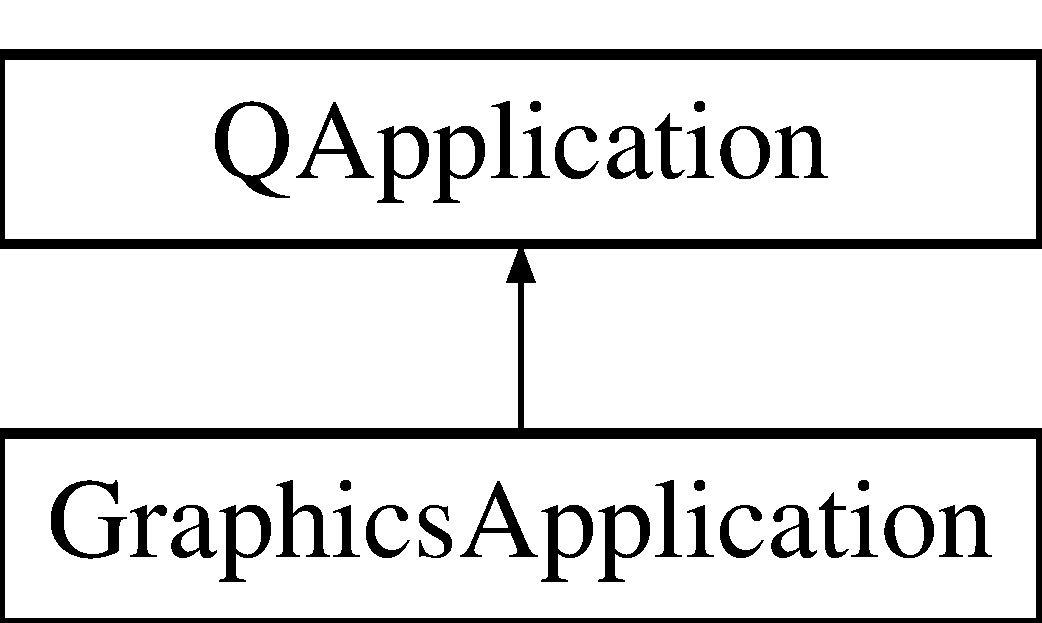
\includegraphics[height=2.000000cm]{class_d_o_1_1_graphics_application}
\end{center}
\end{figure}
\subsection*{Public Slots}
\begin{DoxyCompactItemize}
\item 
\hypertarget{class_d_o_1_1_graphics_application_a91ede8552c45e54ff580346a1facd3e1}{void {\bfseries create\-Painting\-Window} (int w, int h, const Q\-String \&window\-Title, int x, int \hyperlink{group___channel_accessors_gac90c52c5b3a7b2a7e3761e6e84f25778}{y})}\label{class_d_o_1_1_graphics_application_a91ede8552c45e54ff580346a1facd3e1}

\item 
\hypertarget{class_d_o_1_1_graphics_application_abf7475aa077a1f00ac79d6d91870c605}{void {\bfseries create\-Open\-G\-L\-Window} (int w, int h, const Q\-String \&window\-Title, int x, int \hyperlink{group___channel_accessors_gac90c52c5b3a7b2a7e3761e6e84f25778}{y})}\label{class_d_o_1_1_graphics_application_abf7475aa077a1f00ac79d6d91870c605}

\item 
\hypertarget{class_d_o_1_1_graphics_application_a8e47c553a48b897d1a3c084808ec5cd4}{void {\bfseries create\-Graphics\-View} (int w, int h, const Q\-String \&window\-Title, int x, int \hyperlink{group___channel_accessors_gac90c52c5b3a7b2a7e3761e6e84f25778}{y})}\label{class_d_o_1_1_graphics_application_a8e47c553a48b897d1a3c084808ec5cd4}

\item 
\hypertarget{class_d_o_1_1_graphics_application_a80b900f921a02a88bc75f722495c5fa1}{void {\bfseries set\-Active\-Window} (Q\-Widget $\ast$w)}\label{class_d_o_1_1_graphics_application_a80b900f921a02a88bc75f722495c5fa1}

\item 
\hypertarget{class_d_o_1_1_graphics_application_ade0128cbcddef1b8a1911fc6019f9377}{void {\bfseries close\-Window} (Q\-Widget $\ast$w)}\label{class_d_o_1_1_graphics_application_ade0128cbcddef1b8a1911fc6019f9377}

\item 
\hypertarget{class_d_o_1_1_graphics_application_aeb7aedaa0751a70e7328c2f742b2686c}{void {\bfseries get\-File\-From\-Dialog\-Box} ()}\label{class_d_o_1_1_graphics_application_aeb7aedaa0751a70e7328c2f742b2686c}

\end{DoxyCompactItemize}
\subsection*{Public Member Functions}
\begin{DoxyCompactItemize}
\item 
\hypertarget{class_d_o_1_1_graphics_application_a4eb7658f5775a01f8a1f9e03ffd75bd9}{{\bfseries Graphics\-Application} (int argc, char $\ast$$\ast$argv)}\label{class_d_o_1_1_graphics_application_a4eb7658f5775a01f8a1f9e03ffd75bd9}

\item 
\hypertarget{class_d_o_1_1_graphics_application_ad3db22dd49862e1f75afe856e6e89d1b}{bool {\bfseries active\-Window\-Is\-Visible} ()}\label{class_d_o_1_1_graphics_application_ad3db22dd49862e1f75afe856e6e89d1b}

\item 
\hypertarget{class_d_o_1_1_graphics_application_a3db095f1054de65a90af3d2631fac067}{void {\bfseries connect\-Window\-I\-O\-Events\-To\-User\-Thread} (Q\-Widget $\ast$w)}\label{class_d_o_1_1_graphics_application_a3db095f1054de65a90af3d2631fac067}

\item 
\hypertarget{class_d_o_1_1_graphics_application_ace71abe08c7012724571fed56e7e0e27}{void {\bfseries connect\-All\-Windows\-I\-O\-Events\-To\-User\-Thread} ()}\label{class_d_o_1_1_graphics_application_ace71abe08c7012724571fed56e7e0e27}

\item 
\hypertarget{class_d_o_1_1_graphics_application_aa9107742e1cddc2c5fc3854151e2e793}{void {\bfseries disconnect\-All\-Windows\-I\-O\-Events\-To\-User\-Thread} ()}\label{class_d_o_1_1_graphics_application_aa9107742e1cddc2c5fc3854151e2e793}

\end{DoxyCompactItemize}
\subsection*{Public Attributes}
\begin{DoxyCompactItemize}
\item 
\hypertarget{class_d_o_1_1_graphics_application_acd43bf2c420526decde3e16bca3b34d1}{\hyperlink{class_d_o_1_1_user_thread}{User\-Thread} {\bfseries user\-Thread}}\label{class_d_o_1_1_graphics_application_acd43bf2c420526decde3e16bca3b34d1}

\item 
\hypertarget{class_d_o_1_1_graphics_application_ae75bc8ab11de0993ec82b0dd4a26d521}{Q\-List$<$ Q\-Pointer$<$ Q\-Widget $>$ $>$ {\bfseries created\-Windows}}\label{class_d_o_1_1_graphics_application_ae75bc8ab11de0993ec82b0dd4a26d521}

\item 
\hypertarget{class_d_o_1_1_graphics_application_add8fca3b038b4747c6554c0f64cda1dc}{Q\-Pointer$<$ Q\-Widget $>$ {\bfseries active\-Window}}\label{class_d_o_1_1_graphics_application_add8fca3b038b4747c6554c0f64cda1dc}

\item 
\hypertarget{class_d_o_1_1_graphics_application_a5f689b51b1b814abf7df7dbc0f83f49d}{\hyperlink{struct_d_o_1_1_interactive_box}{Interactive\-Box} {\bfseries interactive\-Box}}\label{class_d_o_1_1_graphics_application_a5f689b51b1b814abf7df7dbc0f83f49d}

\item 
\hypertarget{class_d_o_1_1_graphics_application_af6f9da7af5126b3f589fc5ff8b002335}{Q\-Mutex {\bfseries mutex}}\label{class_d_o_1_1_graphics_application_af6f9da7af5126b3f589fc5ff8b002335}

\end{DoxyCompactItemize}


\subsection{Detailed Description}
Q\-Application-\/derived class This graphic application establishes communication between the user drawing commands and the windows. 

The documentation for this class was generated from the following file\-:\begin{DoxyCompactItemize}
\item 
src/\-D\-O/\-Graphics/\-Derived\-Q\-Objects/\hyperlink{_graphics_application_8hpp}{Graphics\-Application.\-hpp}\end{DoxyCompactItemize}

\hypertarget{class_d_o_1_1_graphics_view}{\section{Graphics\-View Class Reference}
\label{class_d_o_1_1_graphics_view}\index{Graphics\-View@{Graphics\-View}}
}


Q\-Graphics\-View-\/derived class used to view interactively images.  




{\ttfamily \#include $<$Graphics\-View.\-hpp$>$}

Inheritance diagram for Graphics\-View\-:\begin{figure}[H]
\begin{center}
\leavevmode
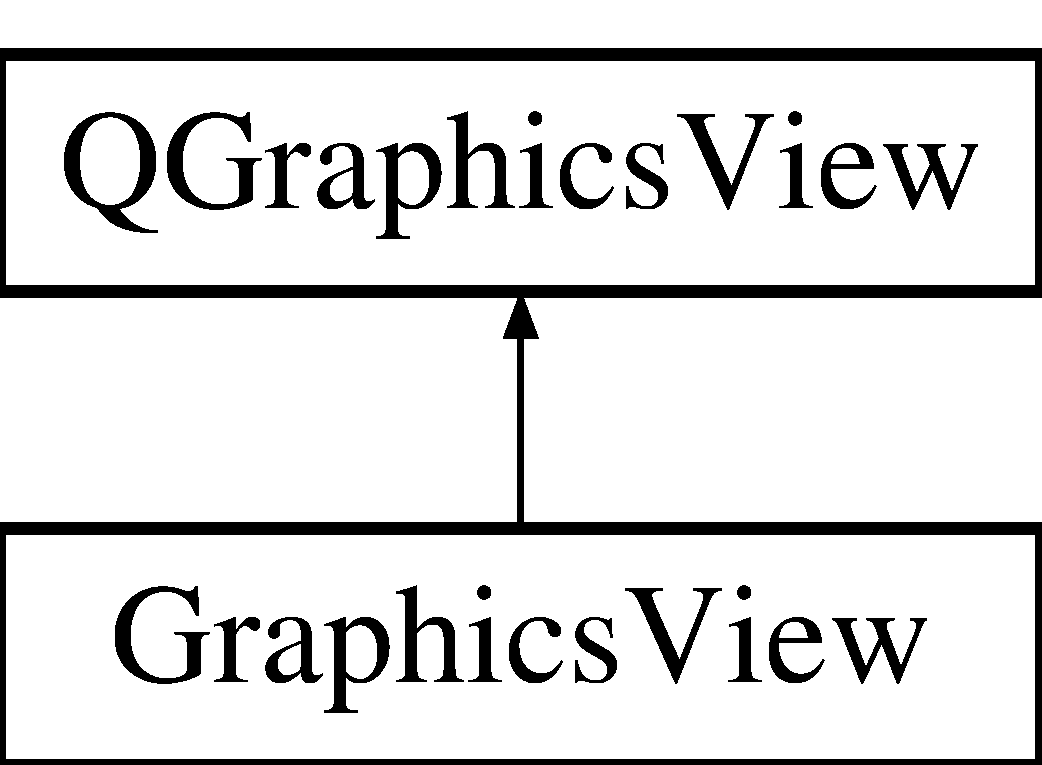
\includegraphics[height=2.000000cm]{class_d_o_1_1_graphics_view}
\end{center}
\end{figure}
\subsection*{Public Slots}
\begin{DoxyCompactItemize}
\item 
\hypertarget{class_d_o_1_1_graphics_view_a08697b6029853534915c9e3ecdc15c28}{void {\bfseries add\-Item} (Q\-Graphics\-Item $\ast$item, Q\-Graphics\-Item $\ast$parent=0)}\label{class_d_o_1_1_graphics_view_a08697b6029853534915c9e3ecdc15c28}

\item 
\hypertarget{class_d_o_1_1_graphics_view_a34f377b6ef0f039b94282e6da9c0df08}{void {\bfseries add\-Image\-Item} (const Q\-Image \&image, bool random\-Pos=false)}\label{class_d_o_1_1_graphics_view_a34f377b6ef0f039b94282e6da9c0df08}

\item 
\hypertarget{class_d_o_1_1_graphics_view_a743cbf84024a728d5ec8f20fadf859d0}{void {\bfseries draw\-Point\-On\-Pixmap\-Item} (int x, int \hyperlink{group___channel_accessors_gac90c52c5b3a7b2a7e3761e6e84f25778}{y}, const Q\-Color \&c, Q\-Graphics\-Pixmap\-Item $\ast$pix\-Item)}\label{class_d_o_1_1_graphics_view_a743cbf84024a728d5ec8f20fadf859d0}

\end{DoxyCompactItemize}
\subsection*{Signals}
\begin{DoxyCompactItemize}
\item 
\hypertarget{class_d_o_1_1_graphics_view_a211d59c0a6baf6072e762c542472efe6}{void {\bfseries pressed\-Mouse\-Buttons} (int x, int \hyperlink{group___channel_accessors_gac90c52c5b3a7b2a7e3761e6e84f25778}{y}, Qt\-::\-Mouse\-Buttons buttons)}\label{class_d_o_1_1_graphics_view_a211d59c0a6baf6072e762c542472efe6}

\item 
\hypertarget{class_d_o_1_1_graphics_view_aa6e288186f3b4d8668cbcb77d4d5cc71}{void {\bfseries released\-Mouse\-Buttons} (int x, int \hyperlink{group___channel_accessors_gac90c52c5b3a7b2a7e3761e6e84f25778}{y}, Qt\-::\-Mouse\-Buttons buttons)}\label{class_d_o_1_1_graphics_view_aa6e288186f3b4d8668cbcb77d4d5cc71}

\item 
\hypertarget{class_d_o_1_1_graphics_view_af3120a375a321654553779cf030a9508}{void {\bfseries pressed\-Key} (int key)}\label{class_d_o_1_1_graphics_view_af3120a375a321654553779cf030a9508}

\item 
\hypertarget{class_d_o_1_1_graphics_view_ac80bf1948c09a26181b72cb51f4ea4c3}{void {\bfseries released\-Key} (int key)}\label{class_d_o_1_1_graphics_view_ac80bf1948c09a26181b72cb51f4ea4c3}

\item 
\hypertarget{class_d_o_1_1_graphics_view_a497371cbad118b80dc07aa5c288f2573}{void {\bfseries send\-Event} (\hyperlink{struct_d_o_1_1_event}{Event} e)}\label{class_d_o_1_1_graphics_view_a497371cbad118b80dc07aa5c288f2573}

\end{DoxyCompactItemize}
\subsection*{Public Member Functions}
\begin{DoxyCompactItemize}
\item 
\hypertarget{class_d_o_1_1_graphics_view_a99b0aad23396733b0d8d2c859e9a046b}{{\bfseries Graphics\-View} (int width, int height, const Q\-String \&window\-Title=\char`\"{}D\-O++\char`\"{}, int x=-\/1, int \hyperlink{group___channel_accessors_gac90c52c5b3a7b2a7e3761e6e84f25778}{y}=-\/1, Q\-Widget $\ast$parent=0)}\label{class_d_o_1_1_graphics_view_a99b0aad23396733b0d8d2c859e9a046b}

\item 
\hypertarget{class_d_o_1_1_graphics_view_abad4cda0b2ed3e149d7da9923cd79f43}{void {\bfseries activate\-Open\-G\-L} ()}\label{class_d_o_1_1_graphics_view_abad4cda0b2ed3e149d7da9923cd79f43}

\item 
\hypertarget{class_d_o_1_1_graphics_view_aa33de3fac6475fcdd725a2ca8ad62d4e}{Q\-Graphics\-Item $\ast$ {\bfseries last\-Added\-Item} ()}\label{class_d_o_1_1_graphics_view_aa33de3fac6475fcdd725a2ca8ad62d4e}

\end{DoxyCompactItemize}
\subsection*{Protected Member Functions}
\begin{DoxyCompactItemize}
\item 
\hypertarget{class_d_o_1_1_graphics_view_ad2272e344e46519f026cd02f419884f1}{void {\bfseries mouse\-Press\-Event} (Q\-Mouse\-Event $\ast$event)}\label{class_d_o_1_1_graphics_view_ad2272e344e46519f026cd02f419884f1}

\item 
\hypertarget{class_d_o_1_1_graphics_view_a35226f6549add1ff837c65888fcd00fc}{void {\bfseries mouse\-Release\-Event} (Q\-Mouse\-Event $\ast$event)}\label{class_d_o_1_1_graphics_view_a35226f6549add1ff837c65888fcd00fc}

\item 
\hypertarget{class_d_o_1_1_graphics_view_abc61c05ed30a94d66ab715c718532c03}{void {\bfseries wheel\-Event} (Q\-Wheel\-Event $\ast$)}\label{class_d_o_1_1_graphics_view_abc61c05ed30a94d66ab715c718532c03}

\item 
\hypertarget{class_d_o_1_1_graphics_view_adf2e9d5e456a754a5459e8435b0b094b}{void {\bfseries key\-Press\-Event} (Q\-Key\-Event $\ast$event)}\label{class_d_o_1_1_graphics_view_adf2e9d5e456a754a5459e8435b0b094b}

\item 
\hypertarget{class_d_o_1_1_graphics_view_a5de2bd09256045c0b96e5a0be780fa85}{void {\bfseries close\-Event} (Q\-Close\-Event $\ast$event)}\label{class_d_o_1_1_graphics_view_a5de2bd09256045c0b96e5a0be780fa85}

\end{DoxyCompactItemize}


\subsection{Detailed Description}
Q\-Graphics\-View-\/derived class used to view interactively images. 

The documentation for this class was generated from the following file\-:\begin{DoxyCompactItemize}
\item 
src/\-D\-O/\-Graphics/\-Derived\-Q\-Objects/\hyperlink{_graphics_view_8hpp}{Graphics\-View.\-hpp}\end{DoxyCompactItemize}

\hypertarget{struct_d_o_1_1_gray}{\section{Gray Struct Reference}
\label{struct_d_o_1_1_gray}\index{Gray@{Gray}}
}


Grayscale color space.  




{\ttfamily \#include $<$Color.\-hpp$>$}



\subsection{Detailed Description}
Grayscale color space. 

The documentation for this struct was generated from the following file\-:\begin{DoxyCompactItemize}
\item 
src/\-D\-O/\-Core/\hyperlink{_color_8hpp}{Color.\-hpp}\end{DoxyCompactItemize}

\hypertarget{struct_d_o_1_1_h}{\section{H Struct Reference}
\label{struct_d_o_1_1_h}\index{H@{H}}
}


Hue channel name (H\-S\-V).  




{\ttfamily \#include $<$Color.\-hpp$>$}



\subsection{Detailed Description}
Hue channel name (H\-S\-V). 

The documentation for this struct was generated from the following file\-:\begin{DoxyCompactItemize}
\item 
src/\-D\-O/\-Core/\hyperlink{_color_8hpp}{Color.\-hpp}\end{DoxyCompactItemize}

\hypertarget{class_d_o_1_1_high_res_timer}{\section{High\-Res\-Timer Class Reference}
\label{class_d_o_1_1_high_res_timer}\index{High\-Res\-Timer@{High\-Res\-Timer}}
}


\hyperlink{class_d_o_1_1_timer}{Timer} class with microsecond accuracy.  




{\ttfamily \#include $<$Timer.\-hpp$>$}

\subsection*{Public Member Functions}
\begin{DoxyCompactItemize}
\item 
\hypertarget{class_d_o_1_1_high_res_timer_a22ee094ca3f45aa4156b97d34fe678bf}{void {\bfseries restart} ()}\label{class_d_o_1_1_high_res_timer_a22ee094ca3f45aa4156b97d34fe678bf}

\item 
\hypertarget{class_d_o_1_1_high_res_timer_af4dbcc0b93d74e5fb7100c4299f9ec20}{double {\bfseries elapsed\-Ms} ()}\label{class_d_o_1_1_high_res_timer_af4dbcc0b93d74e5fb7100c4299f9ec20}

\end{DoxyCompactItemize}
\subsection*{Public Attributes}
\begin{DoxyCompactItemize}
\item 
\hypertarget{class_d_o_1_1_high_res_timer_a2ea9282fd2003b9e952e0d2bb54e48c7}{timeval {\bfseries start\-\_\-}}\label{class_d_o_1_1_high_res_timer_a2ea9282fd2003b9e952e0d2bb54e48c7}

\item 
\hypertarget{class_d_o_1_1_high_res_timer_a1ce1b9ff5082e17ac8a6679b7b8df5a4}{timeval {\bfseries end\-\_\-}}\label{class_d_o_1_1_high_res_timer_a1ce1b9ff5082e17ac8a6679b7b8df5a4}

\item 
\hypertarget{class_d_o_1_1_high_res_timer_ac0935164e30e3396a46e9494efb83fe7}{double {\bfseries elapsed\-\_\-}}\label{class_d_o_1_1_high_res_timer_ac0935164e30e3396a46e9494efb83fe7}

\end{DoxyCompactItemize}


\subsection{Detailed Description}
\hyperlink{class_d_o_1_1_timer}{Timer} class with microsecond accuracy. 

The documentation for this class was generated from the following file\-:\begin{DoxyCompactItemize}
\item 
src/\-D\-O/\-Core/\hyperlink{_timer_8hpp}{Timer.\-hpp}\end{DoxyCompactItemize}

\hypertarget{class_d_o_1_1_image}{\section{Image$<$ Color, N $>$ Class Template Reference}
\label{class_d_o_1_1_image}\index{Image$<$ Color, N $>$@{Image$<$ Color, N $>$}}
}


The forward declaration of the image class.  




{\ttfamily \#include $<$Image.\-hpp$>$}

Inheritance diagram for Image$<$ Color, N $>$\-:\begin{figure}[H]
\begin{center}
\leavevmode
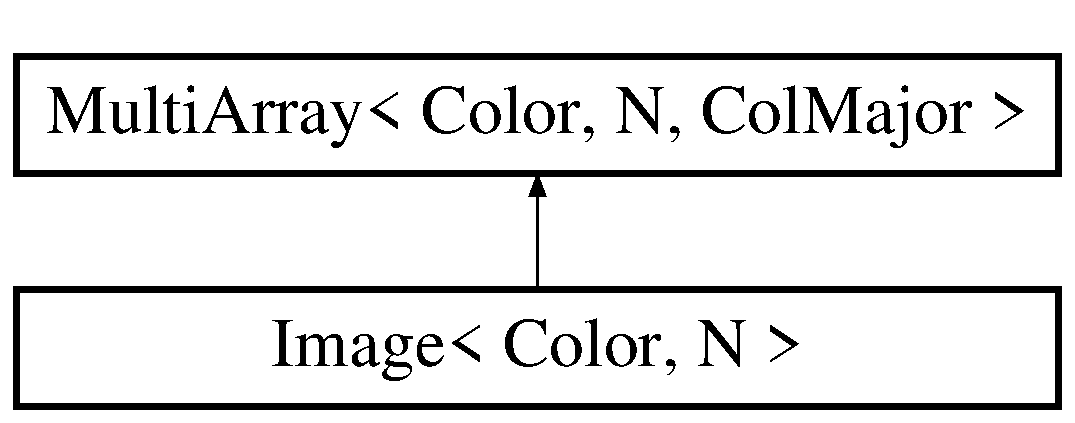
\includegraphics[height=2.000000cm]{class_d_o_1_1_image}
\end{center}
\end{figure}
\subsection*{Public Types}
\begin{DoxyCompactItemize}
\item 
\hypertarget{class_d_o_1_1_image_abbab566abe3e8de5e0b8b8d3ca150a0c}{typedef \hyperlink{class_d_o_1_1_multi_array_a566f0c85cbe372baeec72065fc245842}{Base\-::\-Vector} \hyperlink{class_d_o_1_1_image_abbab566abe3e8de5e0b8b8d3ca150a0c}{Vector}}\label{class_d_o_1_1_image_abbab566abe3e8de5e0b8b8d3ca150a0c}

\begin{DoxyCompactList}\small\item\em N-\/dimensional integral vector type. \end{DoxyCompactList}\end{DoxyCompactItemize}
\subsection*{Public Member Functions}
\begin{DoxyCompactItemize}
\item 
\hypertarget{class_d_o_1_1_image_a66d0d6da3b89580352c28d37b57df5bb}{\hyperlink{class_d_o_1_1_image_a66d0d6da3b89580352c28d37b57df5bb}{Image} ()}\label{class_d_o_1_1_image_a66d0d6da3b89580352c28d37b57df5bb}

\begin{DoxyCompactList}\small\item\em Default constructor. \end{DoxyCompactList}\item 
\hypertarget{class_d_o_1_1_image_aa97e04e962349b89c734dbe20738db24}{\hyperlink{class_d_o_1_1_image_aa97e04e962349b89c734dbe20738db24}{Image} (const \hyperlink{class_d_o_1_1_image_abbab566abe3e8de5e0b8b8d3ca150a0c}{Vector} \&\hyperlink{class_d_o_1_1_multi_array_a15f0ce2877b385c9505f042faa705694}{sizes})}\label{class_d_o_1_1_image_aa97e04e962349b89c734dbe20738db24}

\begin{DoxyCompactList}\small\item\em Constructor with specified sizes. \end{DoxyCompactList}\item 
\hypertarget{class_d_o_1_1_image_a41991711658b8e1686706ced4a439a1c}{\hyperlink{class_d_o_1_1_image_a41991711658b8e1686706ced4a439a1c}{Image} (\hyperlink{class_d_o_1_1_color}{Color} $\ast$\hyperlink{class_d_o_1_1_multi_array_a36e4d11a00a3572c87bf7e913e9b5ca1}{data}, const \hyperlink{class_d_o_1_1_image_abbab566abe3e8de5e0b8b8d3ca150a0c}{Vector} \&\hyperlink{class_d_o_1_1_multi_array_a15f0ce2877b385c9505f042faa705694}{sizes})}\label{class_d_o_1_1_image_a41991711658b8e1686706ced4a439a1c}

\begin{DoxyCompactList}\small\item\em Constructor which wraps raw data. \end{DoxyCompactList}\item 
\hypertarget{class_d_o_1_1_image_af01766f2360b125ef9131ad1c613c013}{\hyperlink{class_d_o_1_1_image_af01766f2360b125ef9131ad1c613c013}{Image} (int \hyperlink{class_d_o_1_1_image_a369399896761e31ae71db57fdd0ba431}{width}, int \hyperlink{class_d_o_1_1_image_ae26bcfe2f33f5873dbdfb6948cf1f59f}{height})}\label{class_d_o_1_1_image_af01766f2360b125ef9131ad1c613c013}

\begin{DoxyCompactList}\small\item\em Constructor with specified sizes. \end{DoxyCompactList}\item 
\hypertarget{class_d_o_1_1_image_ab4c9fa2662875ab1542a5c01ed74373f}{\hyperlink{class_d_o_1_1_image_ab4c9fa2662875ab1542a5c01ed74373f}{Image} (int \hyperlink{class_d_o_1_1_image_a369399896761e31ae71db57fdd0ba431}{width}, int \hyperlink{class_d_o_1_1_image_ae26bcfe2f33f5873dbdfb6948cf1f59f}{height}, int \hyperlink{class_d_o_1_1_image_a3275d1392d01b26af1c8cd52b0d10745}{depth})}\label{class_d_o_1_1_image_ab4c9fa2662875ab1542a5c01ed74373f}

\begin{DoxyCompactList}\small\item\em Constructor with specified sizes. \end{DoxyCompactList}\item 
\hypertarget{class_d_o_1_1_image_a03040d6426bcf2fcd6a7d731d3534796}{\hyperlink{class_d_o_1_1_image_a03040d6426bcf2fcd6a7d731d3534796}{Image} (const \hyperlink{class_d_o_1_1_multi_array}{Base} \&x)}\label{class_d_o_1_1_image_a03040d6426bcf2fcd6a7d731d3534796}

\begin{DoxyCompactList}\small\item\em Copy constructor. \end{DoxyCompactList}\item 
\hypertarget{class_d_o_1_1_image_aaa0c10be1945418c23ef52974a4dadaa}{const \hyperlink{class_d_o_1_1_image}{Image} \& \hyperlink{class_d_o_1_1_image_aaa0c10be1945418c23ef52974a4dadaa}{operator=} (const \hyperlink{class_d_o_1_1_image}{Image} \&I)}\label{class_d_o_1_1_image_aaa0c10be1945418c23ef52974a4dadaa}

\begin{DoxyCompactList}\small\item\em Assignment operators. \end{DoxyCompactList}\item 
\hypertarget{class_d_o_1_1_image_a369399896761e31ae71db57fdd0ba431}{int \hyperlink{class_d_o_1_1_image_a369399896761e31ae71db57fdd0ba431}{width} () const }\label{class_d_o_1_1_image_a369399896761e31ae71db57fdd0ba431}

\begin{DoxyCompactList}\small\item\em Constant width accessor. \end{DoxyCompactList}\item 
\hypertarget{class_d_o_1_1_image_ae26bcfe2f33f5873dbdfb6948cf1f59f}{int \hyperlink{class_d_o_1_1_image_ae26bcfe2f33f5873dbdfb6948cf1f59f}{height} () const }\label{class_d_o_1_1_image_ae26bcfe2f33f5873dbdfb6948cf1f59f}

\begin{DoxyCompactList}\small\item\em Constant height accessor. \end{DoxyCompactList}\item 
\hypertarget{class_d_o_1_1_image_a3275d1392d01b26af1c8cd52b0d10745}{int \hyperlink{class_d_o_1_1_image_a3275d1392d01b26af1c8cd52b0d10745}{depth} () const }\label{class_d_o_1_1_image_a3275d1392d01b26af1c8cd52b0d10745}

\begin{DoxyCompactList}\small\item\em Constant depth accessor (only for volumetric image.) \end{DoxyCompactList}\item 
\hypertarget{class_d_o_1_1_image_a3b35c07b31609437c194be2614e2e594}{{\footnotesize template$<$typename Color2 $>$ }\\\hyperlink{class_d_o_1_1_image}{Image}$<$ Color2, N $>$ \hyperlink{class_d_o_1_1_image_a3b35c07b31609437c194be2614e2e594}{convert} () const }\label{class_d_o_1_1_image_a3b35c07b31609437c194be2614e2e594}

\begin{DoxyCompactList}\small\item\em \hyperlink{class_d_o_1_1_color}{Color} conversion methods. \end{DoxyCompactList}\end{DoxyCompactItemize}


\subsection{Detailed Description}
\subsubsection*{template$<$typename Color, int N = 2$>$class D\-O\-::\-Image$<$ Color, N $>$}

The forward declaration of the image class. 

The image class. 

The documentation for this class was generated from the following file\-:\begin{DoxyCompactItemize}
\item 
src/\-D\-O/\-Core/\hyperlink{_image_8hpp}{Image.\-hpp}\end{DoxyCompactItemize}

\hypertarget{struct_d_o_1_1_meta_1_1_index_of}{\section{Index\-Of$<$ Vector, T $>$ Struct Template Reference}
\label{struct_d_o_1_1_meta_1_1_index_of}\index{Index\-Of$<$ Vector, T $>$@{Index\-Of$<$ Vector, T $>$}}
}


Index getter for vector of types.  




{\ttfamily \#include $<$Meta.\-hpp$>$}



\subsection{Detailed Description}
\subsubsection*{template$<$typename Vector, typename T$>$struct D\-O\-::\-Meta\-::\-Index\-Of$<$ Vector, T $>$}

Index getter for vector of types. 

The documentation for this struct was generated from the following file\-:\begin{DoxyCompactItemize}
\item 
src/\-D\-O/\-Core/\hyperlink{_meta_8hpp}{Meta.\-hpp}\end{DoxyCompactItemize}

\hypertarget{struct_d_o_1_1_meta_1_1_index_of_3_01_vector3_3_01_t0_00_01_t1_00_01_t2_01_4_00_01_t0_01_4}{\section{Index\-Of$<$ Vector3$<$ T0, T1, T2 $>$, T0 $>$ Struct Template Reference}
\label{struct_d_o_1_1_meta_1_1_index_of_3_01_vector3_3_01_t0_00_01_t1_00_01_t2_01_4_00_01_t0_01_4}\index{Index\-Of$<$ Vector3$<$ T0, T1, T2 $>$, T0 $>$@{Index\-Of$<$ Vector3$<$ T0, T1, T2 $>$, T0 $>$}}
}


Specialized index getter of type T0 for \hyperlink{struct_d_o_1_1_meta_1_1_vector3}{Vector3}.  




{\ttfamily \#include $<$Meta.\-hpp$>$}

\subsection*{Public Types}
\begin{DoxyCompactItemize}
\item 
enum \{ {\bfseries value} = 0
 \}
\end{DoxyCompactItemize}


\subsection{Detailed Description}
\subsubsection*{template$<$typename T0, typename T1, typename T2$>$struct D\-O\-::\-Meta\-::\-Index\-Of$<$ Vector3$<$ T0, T1, T2 $>$, T0 $>$}

Specialized index getter of type T0 for \hyperlink{struct_d_o_1_1_meta_1_1_vector3}{Vector3}. 

The documentation for this struct was generated from the following file\-:\begin{DoxyCompactItemize}
\item 
src/\-D\-O/\-Core/\hyperlink{_meta_8hpp}{Meta.\-hpp}\end{DoxyCompactItemize}

\hypertarget{struct_d_o_1_1_meta_1_1_index_of_3_01_vector3_3_01_t0_00_01_t1_00_01_t2_01_4_00_01_t1_01_4}{\section{Index\-Of$<$ Vector3$<$ T0, T1, T2 $>$, T1 $>$ Struct Template Reference}
\label{struct_d_o_1_1_meta_1_1_index_of_3_01_vector3_3_01_t0_00_01_t1_00_01_t2_01_4_00_01_t1_01_4}\index{Index\-Of$<$ Vector3$<$ T0, T1, T2 $>$, T1 $>$@{Index\-Of$<$ Vector3$<$ T0, T1, T2 $>$, T1 $>$}}
}


Specialized index getter of type T1 for \hyperlink{struct_d_o_1_1_meta_1_1_vector3}{Vector3}.  




{\ttfamily \#include $<$Meta.\-hpp$>$}

\subsection*{Public Types}
\begin{DoxyCompactItemize}
\item 
enum \{ {\bfseries value} = 1
 \}
\end{DoxyCompactItemize}


\subsection{Detailed Description}
\subsubsection*{template$<$typename T0, typename T1, typename T2$>$struct D\-O\-::\-Meta\-::\-Index\-Of$<$ Vector3$<$ T0, T1, T2 $>$, T1 $>$}

Specialized index getter of type T1 for \hyperlink{struct_d_o_1_1_meta_1_1_vector3}{Vector3}. 

The documentation for this struct was generated from the following file\-:\begin{DoxyCompactItemize}
\item 
src/\-D\-O/\-Core/\hyperlink{_meta_8hpp}{Meta.\-hpp}\end{DoxyCompactItemize}

\hypertarget{struct_d_o_1_1_meta_1_1_index_of_3_01_vector3_3_01_t0_00_01_t1_00_01_t2_01_4_00_01_t2_01_4}{\section{Index\-Of$<$ Vector3$<$ T0, T1, T2 $>$, T2 $>$ Struct Template Reference}
\label{struct_d_o_1_1_meta_1_1_index_of_3_01_vector3_3_01_t0_00_01_t1_00_01_t2_01_4_00_01_t2_01_4}\index{Index\-Of$<$ Vector3$<$ T0, T1, T2 $>$, T2 $>$@{Index\-Of$<$ Vector3$<$ T0, T1, T2 $>$, T2 $>$}}
}


Specialized index getter of type T2 for \hyperlink{struct_d_o_1_1_meta_1_1_vector3}{Vector3}.  




{\ttfamily \#include $<$Meta.\-hpp$>$}

\subsection*{Public Types}
\begin{DoxyCompactItemize}
\item 
enum \{ {\bfseries value} = 2
 \}
\end{DoxyCompactItemize}


\subsection{Detailed Description}
\subsubsection*{template$<$typename T0, typename T1, typename T2$>$struct D\-O\-::\-Meta\-::\-Index\-Of$<$ Vector3$<$ T0, T1, T2 $>$, T2 $>$}

Specialized index getter of type T2 for \hyperlink{struct_d_o_1_1_meta_1_1_vector3}{Vector3}. 

The documentation for this struct was generated from the following file\-:\begin{DoxyCompactItemize}
\item 
src/\-D\-O/\-Core/\hyperlink{_meta_8hpp}{Meta.\-hpp}\end{DoxyCompactItemize}

\hypertarget{struct_d_o_1_1_meta_1_1_index_of_3_01_vector4_3_01_t0_00_01_t1_00_01_t2_00_01_t3_01_4_00_01_t0_01_4}{\section{Index\-Of$<$ Vector4$<$ T0, T1, T2, T3 $>$, T0 $>$ Struct Template Reference}
\label{struct_d_o_1_1_meta_1_1_index_of_3_01_vector4_3_01_t0_00_01_t1_00_01_t2_00_01_t3_01_4_00_01_t0_01_4}\index{Index\-Of$<$ Vector4$<$ T0, T1, T2, T3 $>$, T0 $>$@{Index\-Of$<$ Vector4$<$ T0, T1, T2, T3 $>$, T0 $>$}}
}


Specialized index getter of type T0 for \hyperlink{struct_d_o_1_1_meta_1_1_vector4}{Vector4}.  




{\ttfamily \#include $<$Meta.\-hpp$>$}

\subsection*{Public Types}
\begin{DoxyCompactItemize}
\item 
enum \{ {\bfseries value} = 0
 \}
\end{DoxyCompactItemize}


\subsection{Detailed Description}
\subsubsection*{template$<$typename T0, typename T1, typename T2, typename T3$>$struct D\-O\-::\-Meta\-::\-Index\-Of$<$ Vector4$<$ T0, T1, T2, T3 $>$, T0 $>$}

Specialized index getter of type T0 for \hyperlink{struct_d_o_1_1_meta_1_1_vector4}{Vector4}. 

The documentation for this struct was generated from the following file\-:\begin{DoxyCompactItemize}
\item 
src/\-D\-O/\-Core/\hyperlink{_meta_8hpp}{Meta.\-hpp}\end{DoxyCompactItemize}

\hypertarget{struct_d_o_1_1_meta_1_1_index_of_3_01_vector4_3_01_t0_00_01_t1_00_01_t2_00_01_t3_01_4_00_01_t1_01_4}{\section{Index\-Of$<$ Vector4$<$ T0, T1, T2, T3 $>$, T1 $>$ Struct Template Reference}
\label{struct_d_o_1_1_meta_1_1_index_of_3_01_vector4_3_01_t0_00_01_t1_00_01_t2_00_01_t3_01_4_00_01_t1_01_4}\index{Index\-Of$<$ Vector4$<$ T0, T1, T2, T3 $>$, T1 $>$@{Index\-Of$<$ Vector4$<$ T0, T1, T2, T3 $>$, T1 $>$}}
}


Specialized index getter of type T1 for \hyperlink{struct_d_o_1_1_meta_1_1_vector4}{Vector4}.  




{\ttfamily \#include $<$Meta.\-hpp$>$}

\subsection*{Public Types}
\begin{DoxyCompactItemize}
\item 
enum \{ {\bfseries value} = 1
 \}
\end{DoxyCompactItemize}


\subsection{Detailed Description}
\subsubsection*{template$<$typename T0, typename T1, typename T2, typename T3$>$struct D\-O\-::\-Meta\-::\-Index\-Of$<$ Vector4$<$ T0, T1, T2, T3 $>$, T1 $>$}

Specialized index getter of type T1 for \hyperlink{struct_d_o_1_1_meta_1_1_vector4}{Vector4}. 

The documentation for this struct was generated from the following file\-:\begin{DoxyCompactItemize}
\item 
src/\-D\-O/\-Core/\hyperlink{_meta_8hpp}{Meta.\-hpp}\end{DoxyCompactItemize}

\hypertarget{struct_d_o_1_1_meta_1_1_index_of_3_01_vector4_3_01_t0_00_01_t1_00_01_t2_00_01_t3_01_4_00_01_t2_01_4}{\section{Index\-Of$<$ Vector4$<$ T0, T1, T2, T3 $>$, T2 $>$ Struct Template Reference}
\label{struct_d_o_1_1_meta_1_1_index_of_3_01_vector4_3_01_t0_00_01_t1_00_01_t2_00_01_t3_01_4_00_01_t2_01_4}\index{Index\-Of$<$ Vector4$<$ T0, T1, T2, T3 $>$, T2 $>$@{Index\-Of$<$ Vector4$<$ T0, T1, T2, T3 $>$, T2 $>$}}
}


Specialized index getter of type T2 for \hyperlink{struct_d_o_1_1_meta_1_1_vector4}{Vector4}.  




{\ttfamily \#include $<$Meta.\-hpp$>$}

\subsection*{Public Types}
\begin{DoxyCompactItemize}
\item 
enum \{ {\bfseries value} = 2
 \}
\end{DoxyCompactItemize}


\subsection{Detailed Description}
\subsubsection*{template$<$typename T0, typename T1, typename T2, typename T3$>$struct D\-O\-::\-Meta\-::\-Index\-Of$<$ Vector4$<$ T0, T1, T2, T3 $>$, T2 $>$}

Specialized index getter of type T2 for \hyperlink{struct_d_o_1_1_meta_1_1_vector4}{Vector4}. 

The documentation for this struct was generated from the following file\-:\begin{DoxyCompactItemize}
\item 
src/\-D\-O/\-Core/\hyperlink{_meta_8hpp}{Meta.\-hpp}\end{DoxyCompactItemize}

\hypertarget{struct_d_o_1_1_meta_1_1_index_of_3_01_vector4_3_01_t0_00_01_t1_00_01_t2_00_01_t3_01_4_00_01_t3_01_4}{\section{Index\-Of$<$ Vector4$<$ T0, T1, T2, T3 $>$, T3 $>$ Struct Template Reference}
\label{struct_d_o_1_1_meta_1_1_index_of_3_01_vector4_3_01_t0_00_01_t1_00_01_t2_00_01_t3_01_4_00_01_t3_01_4}\index{Index\-Of$<$ Vector4$<$ T0, T1, T2, T3 $>$, T3 $>$@{Index\-Of$<$ Vector4$<$ T0, T1, T2, T3 $>$, T3 $>$}}
}


Specialized index getter of type T3 for \hyperlink{struct_d_o_1_1_meta_1_1_vector4}{Vector4}.  




{\ttfamily \#include $<$Meta.\-hpp$>$}

\subsection*{Public Types}
\begin{DoxyCompactItemize}
\item 
enum \{ {\bfseries value} = 3
 \}
\end{DoxyCompactItemize}


\subsection{Detailed Description}
\subsubsection*{template$<$typename T0, typename T1, typename T2, typename T3$>$struct D\-O\-::\-Meta\-::\-Index\-Of$<$ Vector4$<$ T0, T1, T2, T3 $>$, T3 $>$}

Specialized index getter of type T3 for \hyperlink{struct_d_o_1_1_meta_1_1_vector4}{Vector4}. 

The documentation for this struct was generated from the following file\-:\begin{DoxyCompactItemize}
\item 
src/\-D\-O/\-Core/\hyperlink{_meta_8hpp}{Meta.\-hpp}\end{DoxyCompactItemize}

\hypertarget{struct_d_o_1_1_interactive_box}{\section{Interactive\-Box Struct Reference}
\label{struct_d_o_1_1_interactive_box}\index{Interactive\-Box@{Interactive\-Box}}
}


quick-\/and-\/dirty thing to read file from dialog box.  




{\ttfamily \#include $<$Graphics\-Application.\-hpp$>$}

\subsection*{Public Attributes}
\begin{DoxyCompactItemize}
\item 
\hypertarget{struct_d_o_1_1_interactive_box_a734934801a260897766516dac3a878bd}{Q\-Pixmap {\bfseries pixmap}}\label{struct_d_o_1_1_interactive_box_a734934801a260897766516dac3a878bd}

\item 
\hypertarget{struct_d_o_1_1_interactive_box_aac274af37f5fbaaa2c47d19145cfd856}{Q\-String {\bfseries filename}}\label{struct_d_o_1_1_interactive_box_aac274af37f5fbaaa2c47d19145cfd856}

\end{DoxyCompactItemize}


\subsection{Detailed Description}
quick-\/and-\/dirty thing to read file from dialog box. 

\begin{DoxyRefDesc}{Todo}
\item[\hyperlink{todo__todo000002}{Todo}]See if it can be done in a more elegant way. \end{DoxyRefDesc}


The documentation for this struct was generated from the following file\-:\begin{DoxyCompactItemize}
\item 
src/\-D\-O/\-Graphics/\-Derived\-Q\-Objects/\hyperlink{_graphics_application_8hpp}{Graphics\-Application.\-hpp}\end{DoxyCompactItemize}

\hypertarget{struct_d_o_1_1_meta_1_1_is_same}{\section{Is\-Same$<$ T, U $>$ Struct Template Reference}
\label{struct_d_o_1_1_meta_1_1_is_same}\index{Is\-Same$<$ T, U $>$@{Is\-Same$<$ T, U $>$}}
}


Type equality function.  




{\ttfamily \#include $<$Meta.\-hpp$>$}

\subsection*{Static Public Attributes}
\begin{DoxyCompactItemize}
\item 
static const bool \hyperlink{struct_d_o_1_1_meta_1_1_is_same_a11ddd051208250c32dc4985abcafa86d}{value} = false
\end{DoxyCompactItemize}


\subsection{Detailed Description}
\subsubsection*{template$<$typename T, typename U$>$struct D\-O\-::\-Meta\-::\-Is\-Same$<$ T, U $>$}

Type equality function. 

\subsection{Member Data Documentation}
\hypertarget{struct_d_o_1_1_meta_1_1_is_same_a11ddd051208250c32dc4985abcafa86d}{\index{D\-O\-::\-Meta\-::\-Is\-Same@{D\-O\-::\-Meta\-::\-Is\-Same}!value@{value}}
\index{value@{value}!DO::Meta::IsSame@{D\-O\-::\-Meta\-::\-Is\-Same}}
\subsubsection[{value}]{\setlength{\rightskip}{0pt plus 5cm}const bool value = false\hspace{0.3cm}{\ttfamily [static]}}}\label{struct_d_o_1_1_meta_1_1_is_same_a11ddd051208250c32dc4985abcafa86d}
Default value. 

The documentation for this struct was generated from the following file\-:\begin{DoxyCompactItemize}
\item 
src/\-D\-O/\-Core/\hyperlink{_meta_8hpp}{Meta.\-hpp}\end{DoxyCompactItemize}

\hypertarget{struct_d_o_1_1_meta_1_1_is_same_3_01_t_00_01_t_01_4}{\section{Is\-Same$<$ T, T $>$ Struct Template Reference}
\label{struct_d_o_1_1_meta_1_1_is_same_3_01_t_00_01_t_01_4}\index{Is\-Same$<$ T, T $>$@{Is\-Same$<$ T, T $>$}}
}


Specialized type equality function when the two parameters are equal.  




{\ttfamily \#include $<$Meta.\-hpp$>$}

\subsection*{Static Public Attributes}
\begin{DoxyCompactItemize}
\item 
static const bool \hyperlink{struct_d_o_1_1_meta_1_1_is_same_3_01_t_00_01_t_01_4_a11ddd051208250c32dc4985abcafa86d}{value} = true
\end{DoxyCompactItemize}


\subsection{Detailed Description}
\subsubsection*{template$<$typename T$>$struct D\-O\-::\-Meta\-::\-Is\-Same$<$ T, T $>$}

Specialized type equality function when the two parameters are equal. 

\subsection{Member Data Documentation}
\hypertarget{struct_d_o_1_1_meta_1_1_is_same_3_01_t_00_01_t_01_4_a11ddd051208250c32dc4985abcafa86d}{\index{D\-O\-::\-Meta\-::\-Is\-Same$<$ T, T $>$@{D\-O\-::\-Meta\-::\-Is\-Same$<$ T, T $>$}!value@{value}}
\index{value@{value}!DO::Meta::IsSame< T, T >@{D\-O\-::\-Meta\-::\-Is\-Same$<$ T, T $>$}}
\subsubsection[{value}]{\setlength{\rightskip}{0pt plus 5cm}const bool value = true\hspace{0.3cm}{\ttfamily [static]}}}\label{struct_d_o_1_1_meta_1_1_is_same_3_01_t_00_01_t_01_4_a11ddd051208250c32dc4985abcafa86d}
Logically. 

The documentation for this struct was generated from the following file\-:\begin{DoxyCompactItemize}
\item 
src/\-D\-O/\-Core/\hyperlink{_meta_8hpp}{Meta.\-hpp}\end{DoxyCompactItemize}

\hypertarget{struct_d_o_1_1_k}{\section{K Struct Reference}
\label{struct_d_o_1_1_k}\index{K@{K}}
}


Black channel name (C\-M\-Y\-K).  




{\ttfamily \#include $<$Color.\-hpp$>$}



\subsection{Detailed Description}
Black channel name (C\-M\-Y\-K). 

The documentation for this struct was generated from the following file\-:\begin{DoxyCompactItemize}
\item 
src/\-D\-O/\-Core/\hyperlink{_color_8hpp}{Color.\-hpp}\end{DoxyCompactItemize}

\hypertarget{struct_d_o_1_1_lexicographical_order}{\section{Lexicographical\-Order Struct Reference}
\label{struct_d_o_1_1_lexicographical_order}\index{Lexicographical\-Order@{Lexicographical\-Order}}
}


Lexicographical comparison functor for matrices.  




{\ttfamily \#include $<$Eigen\-Extension.\-hpp$>$}

\subsection*{Public Member Functions}
\begin{DoxyCompactItemize}
\item 
\hypertarget{struct_d_o_1_1_lexicographical_order_a41a012640ffdb9c89e7ed18d92e89443}{{\footnotesize template$<$typename T , int M, int N$>$ }\\bool \hyperlink{struct_d_o_1_1_lexicographical_order_a41a012640ffdb9c89e7ed18d92e89443}{operator()} (const Matrix$<$ T, \hyperlink{struct_d_o_1_1_m}{M}, N $>$ \&m1, const Matrix$<$ T, \hyperlink{struct_d_o_1_1_m}{M}, N $>$ \&m2) const }\label{struct_d_o_1_1_lexicographical_order_a41a012640ffdb9c89e7ed18d92e89443}

\begin{DoxyCompactList}\small\item\em Implementation of the functor. \end{DoxyCompactList}\end{DoxyCompactItemize}


\subsection{Detailed Description}
Lexicographical comparison functor for matrices. 

The documentation for this struct was generated from the following file\-:\begin{DoxyCompactItemize}
\item 
src/\-D\-O/\-Core/\hyperlink{_eigen_extension_8hpp}{Eigen\-Extension.\-hpp}\end{DoxyCompactItemize}

\hypertarget{class_d_o_1_1_locator}{\section{Locator$<$ T, N, Storage\-Order $>$ Class Template Reference}
\label{class_d_o_1_1_locator}\index{Locator$<$ T, N, Storage\-Order $>$@{Locator$<$ T, N, Storage\-Order $>$}}
}


N-\/dimensional iterator class.  




{\ttfamily \#include $<$Locator.\-hpp$>$}

Inheritance diagram for Locator$<$ T, N, Storage\-Order $>$\-:\begin{figure}[H]
\begin{center}
\leavevmode
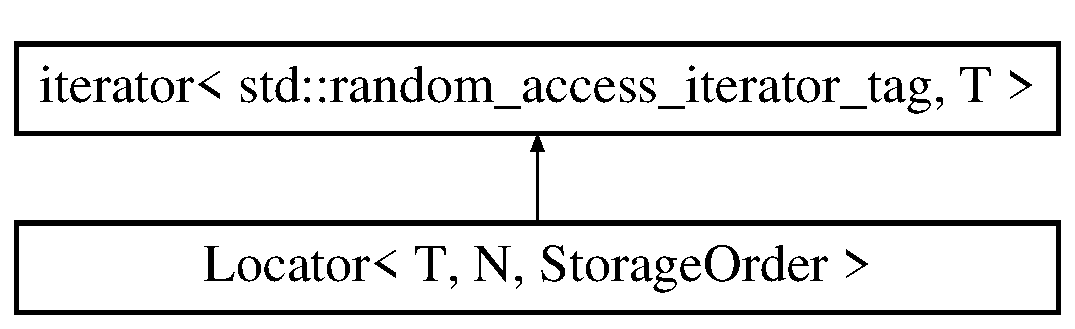
\includegraphics[height=2.000000cm]{class_d_o_1_1_locator}
\end{center}
\end{figure}
\subsection*{Public Types}
\begin{DoxyCompactItemize}
\item 
\hypertarget{class_d_o_1_1_locator_a758d02a5183e542558cd2f7ad65c683c}{typedef Base\-::value\-\_\-type \hyperlink{class_d_o_1_1_locator_a758d02a5183e542558cd2f7ad65c683c}{value\-\_\-type}}\label{class_d_o_1_1_locator_a758d02a5183e542558cd2f7ad65c683c}

\begin{DoxyCompactList}\small\item\em value\-\_\-type \end{DoxyCompactList}\item 
\hypertarget{class_d_o_1_1_locator_aa4336e7fd692b20bda7b7227fa9c9f55}{typedef Base\-::difference\-\_\-type \hyperlink{class_d_o_1_1_locator_aa4336e7fd692b20bda7b7227fa9c9f55}{difference\-\_\-type}}\label{class_d_o_1_1_locator_aa4336e7fd692b20bda7b7227fa9c9f55}

\begin{DoxyCompactList}\small\item\em difference\-\_\-type \end{DoxyCompactList}\item 
\hypertarget{class_d_o_1_1_locator_aa2158dc2d25210ef557a40d3b8a521e3}{typedef Base\-::pointer \hyperlink{class_d_o_1_1_locator_aa2158dc2d25210ef557a40d3b8a521e3}{pointer}}\label{class_d_o_1_1_locator_aa2158dc2d25210ef557a40d3b8a521e3}

\begin{DoxyCompactList}\small\item\em pointer \end{DoxyCompactList}\item 
\hypertarget{class_d_o_1_1_locator_abaed3f9c23f38a6baedf841296fa931c}{typedef Base\-::reference \hyperlink{class_d_o_1_1_locator_abaed3f9c23f38a6baedf841296fa931c}{reference}}\label{class_d_o_1_1_locator_abaed3f9c23f38a6baedf841296fa931c}

\begin{DoxyCompactList}\small\item\em reference \end{DoxyCompactList}\item 
\hypertarget{class_d_o_1_1_locator_a61a96ce54a0b0407ce9bdd9d3f0e3934}{typedef Base\-::iterator\-\_\-category \hyperlink{class_d_o_1_1_locator_a61a96ce54a0b0407ce9bdd9d3f0e3934}{iterator\-\_\-category}}\label{class_d_o_1_1_locator_a61a96ce54a0b0407ce9bdd9d3f0e3934}

\begin{DoxyCompactList}\small\item\em iterator\-\_\-category \end{DoxyCompactList}\item 
\hypertarget{class_d_o_1_1_locator_a2b4e7bf0649f420e5db026e79ac499be}{typedef \hyperlink{class_d_o_1_1_locator}{Locator} \hyperlink{class_d_o_1_1_locator_a2b4e7bf0649f420e5db026e79ac499be}{self\-\_\-type}}\label{class_d_o_1_1_locator_a2b4e7bf0649f420e5db026e79ac499be}

\begin{DoxyCompactList}\small\item\em self\-\_\-type \end{DoxyCompactList}\item 
\hypertarget{class_d_o_1_1_locator_ad4305c73fecc71059d7f201539322941}{typedef \hyperlink{class_d_o_1_1_axis_iterator}{Axis\-Iterator}\\*
$<$ \hyperlink{class_d_o_1_1_locator_a758d02a5183e542558cd2f7ad65c683c}{value\-\_\-type}, 0, N, \\*
Storage\-Order $>$ \hyperlink{class_d_o_1_1_locator_ad4305c73fecc71059d7f201539322941}{x\-\_\-iterator}}\label{class_d_o_1_1_locator_ad4305c73fecc71059d7f201539322941}

\begin{DoxyCompactList}\small\item\em x\-\_\-iterator \end{DoxyCompactList}\item 
\hypertarget{class_d_o_1_1_locator_af164507f5d2199608aa38d15634c878b}{typedef \hyperlink{class_d_o_1_1_axis_iterator}{Axis\-Iterator}\\*
$<$ \hyperlink{class_d_o_1_1_locator_a758d02a5183e542558cd2f7ad65c683c}{value\-\_\-type}, 1, N, \\*
Storage\-Order $>$ \hyperlink{class_d_o_1_1_locator_af164507f5d2199608aa38d15634c878b}{y\-\_\-iterator}}\label{class_d_o_1_1_locator_af164507f5d2199608aa38d15634c878b}

\begin{DoxyCompactList}\small\item\em y\-\_\-iterator \end{DoxyCompactList}\item 
\hypertarget{class_d_o_1_1_locator_a252ebfc1dc8bb45458786e358b6dd4cf}{typedef \hyperlink{class_d_o_1_1_axis_iterator}{Axis\-Iterator}\\*
$<$ \hyperlink{class_d_o_1_1_locator_a758d02a5183e542558cd2f7ad65c683c}{value\-\_\-type}, 2, N, \\*
Storage\-Order $>$ \hyperlink{class_d_o_1_1_locator_a252ebfc1dc8bb45458786e358b6dd4cf}{z\-\_\-iterator}}\label{class_d_o_1_1_locator_a252ebfc1dc8bb45458786e358b6dd4cf}

\begin{DoxyCompactList}\small\item\em z\-\_\-iterator \end{DoxyCompactList}\item 
\hypertarget{class_d_o_1_1_locator_ae4fb477425bbeb20329d300396ac2582}{typedef Matrix$<$ int, N, 1 $>$ {\bfseries coord\-\_\-type}}\label{class_d_o_1_1_locator_ae4fb477425bbeb20329d300396ac2582}

\item 
\hypertarget{class_d_o_1_1_locator_aacf98e49e90f9aeead0ff8885fae3ac7}{typedef Matrix$<$ int, N, 1 $>$ \hyperlink{class_d_o_1_1_locator_aacf98e49e90f9aeead0ff8885fae3ac7}{vector\-\_\-type}}\label{class_d_o_1_1_locator_aacf98e49e90f9aeead0ff8885fae3ac7}

\begin{DoxyCompactList}\small\item\em coord\-\_\-type \end{DoxyCompactList}\end{DoxyCompactItemize}
\subsection*{Public Member Functions}
\begin{DoxyCompactItemize}
\item 
\hypertarget{class_d_o_1_1_locator_ab755eccc7041f74d284063d3f44068e9}{\hyperlink{class_d_o_1_1_locator_ab755eccc7041f74d284063d3f44068e9}{Locator} (\hyperlink{class_d_o_1_1_locator_aa2158dc2d25210ef557a40d3b8a521e3}{pointer} pos, const coord\-\_\-type \&\hyperlink{class_d_o_1_1_locator_a097d0e1275ad521eec770c654ae7c11a}{coords}, \hyperlink{class_d_o_1_1_locator_aa2158dc2d25210ef557a40d3b8a521e3}{pointer} first, \hyperlink{class_d_o_1_1_locator_aa2158dc2d25210ef557a40d3b8a521e3}{pointer} last, const \hyperlink{class_d_o_1_1_locator_aacf98e49e90f9aeead0ff8885fae3ac7}{vector\-\_\-type} \&\hyperlink{class_d_o_1_1_locator_a15f0ce2877b385c9505f042faa705694}{sizes}, const \hyperlink{class_d_o_1_1_locator_aacf98e49e90f9aeead0ff8885fae3ac7}{vector\-\_\-type} \&\hyperlink{class_d_o_1_1_locator_a5be6b48ede748b588c237552cbf3b6b8}{strides})}\label{class_d_o_1_1_locator_ab755eccc7041f74d284063d3f44068e9}

\begin{DoxyCompactList}\small\item\em Constructor. \end{DoxyCompactList}\item 
\hypertarget{class_d_o_1_1_locator_ac775564b41ff8e45a763c87708a3a295}{\hyperlink{class_d_o_1_1_locator_ac775564b41ff8e45a763c87708a3a295}{Locator} (const \hyperlink{class_d_o_1_1_locator_a2b4e7bf0649f420e5db026e79ac499be}{self\-\_\-type} \&l)}\label{class_d_o_1_1_locator_ac775564b41ff8e45a763c87708a3a295}

\begin{DoxyCompactList}\small\item\em Copy constructor. \end{DoxyCompactList}\item 
\hypertarget{class_d_o_1_1_locator_aa149c2249879e7727f33688b76bf2c99}{\hyperlink{class_d_o_1_1_locator_abaed3f9c23f38a6baedf841296fa931c}{reference} \hyperlink{class_d_o_1_1_locator_aa149c2249879e7727f33688b76bf2c99}{operator$\ast$} () const }\label{class_d_o_1_1_locator_aa149c2249879e7727f33688b76bf2c99}

\begin{DoxyCompactList}\small\item\em Referencing operator. \end{DoxyCompactList}\item 
\hypertarget{class_d_o_1_1_locator_a33ce448509e9cc0d73861e4c1919c7a7}{\hyperlink{class_d_o_1_1_locator_aa2158dc2d25210ef557a40d3b8a521e3}{pointer} \hyperlink{class_d_o_1_1_locator_a33ce448509e9cc0d73861e4c1919c7a7}{operator-\/$>$} () const }\label{class_d_o_1_1_locator_a33ce448509e9cc0d73861e4c1919c7a7}

\begin{DoxyCompactList}\small\item\em Referencing operator. \end{DoxyCompactList}\item 
\hypertarget{class_d_o_1_1_locator_a32d919fd1ac974efa89582486e7752de}{\hyperlink{class_d_o_1_1_locator_abaed3f9c23f38a6baedf841296fa931c}{reference} \hyperlink{class_d_o_1_1_locator_a32d919fd1ac974efa89582486e7752de}{operator\mbox{[}$\,$\mbox{]}} (int n) const }\label{class_d_o_1_1_locator_a32d919fd1ac974efa89582486e7752de}

\begin{DoxyCompactList}\small\item\em Referencing operator. \end{DoxyCompactList}\item 
\hypertarget{class_d_o_1_1_locator_a6b17c884f5a18c847944e567d71ad97e}{\hyperlink{class_d_o_1_1_locator_abaed3f9c23f38a6baedf841296fa931c}{reference} \hyperlink{class_d_o_1_1_locator_a6b17c884f5a18c847944e567d71ad97e}{operator()} (int i, int j) const }\label{class_d_o_1_1_locator_a6b17c884f5a18c847944e567d71ad97e}

\begin{DoxyCompactList}\small\item\em Particular referencing operators. \end{DoxyCompactList}\item 
\hypertarget{class_d_o_1_1_locator_a5755d4768b1c9721e052999ee4f7aa11}{\hyperlink{class_d_o_1_1_locator_abaed3f9c23f38a6baedf841296fa931c}{reference} \hyperlink{class_d_o_1_1_locator_a5755d4768b1c9721e052999ee4f7aa11}{operator()} (int i, int j, int k) const }\label{class_d_o_1_1_locator_a5755d4768b1c9721e052999ee4f7aa11}

\begin{DoxyCompactList}\small\item\em Particular referencing operators. \end{DoxyCompactList}\item 
\hypertarget{class_d_o_1_1_locator_afa077c4f1e1d6c36024842404b8574bd}{\hyperlink{class_d_o_1_1_locator_abaed3f9c23f38a6baedf841296fa931c}{reference} \hyperlink{class_d_o_1_1_locator_afa077c4f1e1d6c36024842404b8574bd}{operator()} (const \hyperlink{class_d_o_1_1_locator_aacf98e49e90f9aeead0ff8885fae3ac7}{vector\-\_\-type} \&t) const }\label{class_d_o_1_1_locator_afa077c4f1e1d6c36024842404b8574bd}

\begin{DoxyCompactList}\small\item\em Particular referencing operators. \end{DoxyCompactList}\item 
\hypertarget{class_d_o_1_1_locator_a1d893679af27db625590457f8e265eee}{bool \hyperlink{class_d_o_1_1_locator_a1d893679af27db625590457f8e265eee}{operator==} (const \hyperlink{class_d_o_1_1_locator_a2b4e7bf0649f420e5db026e79ac499be}{self\-\_\-type} \&rhs) const }\label{class_d_o_1_1_locator_a1d893679af27db625590457f8e265eee}

\begin{DoxyCompactList}\small\item\em Equality operator. \end{DoxyCompactList}\item 
\hypertarget{class_d_o_1_1_locator_ad3e7caef9082dd2b3f65ea3867336476}{bool \hyperlink{class_d_o_1_1_locator_ad3e7caef9082dd2b3f65ea3867336476}{operator==} (\hyperlink{class_d_o_1_1_locator_aa2158dc2d25210ef557a40d3b8a521e3}{pointer} pos) const }\label{class_d_o_1_1_locator_ad3e7caef9082dd2b3f65ea3867336476}

\begin{DoxyCompactList}\small\item\em Equality operator. \end{DoxyCompactList}\item 
\hypertarget{class_d_o_1_1_locator_afc84f4470aad70894501ebf4900b374f}{bool \hyperlink{class_d_o_1_1_locator_afc84f4470aad70894501ebf4900b374f}{operator!=} (const \hyperlink{class_d_o_1_1_locator_a2b4e7bf0649f420e5db026e79ac499be}{self\-\_\-type} \&rhs) const }\label{class_d_o_1_1_locator_afc84f4470aad70894501ebf4900b374f}

\begin{DoxyCompactList}\small\item\em Inequality operator. \end{DoxyCompactList}\item 
\hypertarget{class_d_o_1_1_locator_ac966afbaec9c16d1cc1bb6819810ab10}{bool \hyperlink{class_d_o_1_1_locator_ac966afbaec9c16d1cc1bb6819810ab10}{operator!=} (\hyperlink{class_d_o_1_1_locator_aa2158dc2d25210ef557a40d3b8a521e3}{pointer} pos) const }\label{class_d_o_1_1_locator_ac966afbaec9c16d1cc1bb6819810ab10}

\begin{DoxyCompactList}\small\item\em Inequality operator. \end{DoxyCompactList}\item 
\hypertarget{class_d_o_1_1_locator_a68c6d6abdde9fef27d6a4f2904212559}{\hyperlink{class_d_o_1_1_locator_a2b4e7bf0649f420e5db026e79ac499be}{self\-\_\-type} \& \hyperlink{class_d_o_1_1_locator_a68c6d6abdde9fef27d6a4f2904212559}{operator++} ()}\label{class_d_o_1_1_locator_a68c6d6abdde9fef27d6a4f2904212559}

\begin{DoxyCompactList}\small\item\em Prefix increment operator. \end{DoxyCompactList}\item 
\hypertarget{class_d_o_1_1_locator_a2fa8797c1ff9e6c2ac6f879a53f60601}{\hyperlink{class_d_o_1_1_locator_a2b4e7bf0649f420e5db026e79ac499be}{self\-\_\-type} \& \hyperlink{class_d_o_1_1_locator_a2fa8797c1ff9e6c2ac6f879a53f60601}{operator-\/-\/} ()}\label{class_d_o_1_1_locator_a2fa8797c1ff9e6c2ac6f879a53f60601}

\begin{DoxyCompactList}\small\item\em Prefix decrement operator. \end{DoxyCompactList}\item 
\hypertarget{class_d_o_1_1_locator_a39f7c37604fd9845ff487b36b6f88602}{\hyperlink{class_d_o_1_1_locator_a2b4e7bf0649f420e5db026e79ac499be}{self\-\_\-type} \hyperlink{class_d_o_1_1_locator_a39f7c37604fd9845ff487b36b6f88602}{operator++} (int)}\label{class_d_o_1_1_locator_a39f7c37604fd9845ff487b36b6f88602}

\begin{DoxyCompactList}\small\item\em Postfix increment operator. \end{DoxyCompactList}\item 
\hypertarget{class_d_o_1_1_locator_ac8142815f977b8411faf27f7b8d804b3}{\hyperlink{class_d_o_1_1_locator_a2b4e7bf0649f420e5db026e79ac499be}{self\-\_\-type} \hyperlink{class_d_o_1_1_locator_ac8142815f977b8411faf27f7b8d804b3}{operator-\/-\/} (int)}\label{class_d_o_1_1_locator_ac8142815f977b8411faf27f7b8d804b3}

\begin{DoxyCompactList}\small\item\em Postfix decrement operator. \end{DoxyCompactList}\item 
\hypertarget{class_d_o_1_1_locator_a6c0808c388428f119495e5ba1d9fbbed}{\hyperlink{class_d_o_1_1_locator_a2b4e7bf0649f420e5db026e79ac499be}{self\-\_\-type} \& {\bfseries operator+=} (const \hyperlink{class_d_o_1_1_locator_aacf98e49e90f9aeead0ff8885fae3ac7}{vector\-\_\-type} \&t)}\label{class_d_o_1_1_locator_a6c0808c388428f119495e5ba1d9fbbed}

\item 
\hypertarget{class_d_o_1_1_locator_afced994f988f5373b78393cab267065a}{\hyperlink{class_d_o_1_1_locator_a2b4e7bf0649f420e5db026e79ac499be}{self\-\_\-type} \& {\bfseries operator-\/=} (const \hyperlink{class_d_o_1_1_locator_aacf98e49e90f9aeead0ff8885fae3ac7}{vector\-\_\-type} \&t)}\label{class_d_o_1_1_locator_afced994f988f5373b78393cab267065a}

\item 
{\footnotesize template$<$int Axis$>$ }\\\hyperlink{class_d_o_1_1_axis_iterator}{Axis\-Iterator}$<$ T, Axis, N, \\*
Storage\-Order $>$ \hyperlink{class_d_o_1_1_locator_a2e106e539d6ba7366e07cc4ae130b29e}{axis} ()
\item 
\hypertarget{class_d_o_1_1_locator_a73957d210565fc1dcf018c748cc7942c}{\hyperlink{class_d_o_1_1_locator_ad4305c73fecc71059d7f201539322941}{x\-\_\-iterator} \hyperlink{class_d_o_1_1_locator_a73957d210565fc1dcf018c748cc7942c}{x} ()}\label{class_d_o_1_1_locator_a73957d210565fc1dcf018c748cc7942c}

\begin{DoxyCompactList}\small\item\em X-\/axis iterator getter. \end{DoxyCompactList}\item 
\hypertarget{class_d_o_1_1_locator_af33cd0d6e05af68f0f5d58c905493f7c}{\hyperlink{class_d_o_1_1_locator_af164507f5d2199608aa38d15634c878b}{y\-\_\-iterator} \hyperlink{class_d_o_1_1_locator_af33cd0d6e05af68f0f5d58c905493f7c}{y} ()}\label{class_d_o_1_1_locator_af33cd0d6e05af68f0f5d58c905493f7c}

\begin{DoxyCompactList}\small\item\em Y-\/axis iterator getter. \end{DoxyCompactList}\item 
\hypertarget{class_d_o_1_1_locator_a67d32d4fcfd807176852b6dfbaa11f74}{\hyperlink{class_d_o_1_1_locator_a252ebfc1dc8bb45458786e358b6dd4cf}{z\-\_\-iterator} \hyperlink{class_d_o_1_1_locator_a67d32d4fcfd807176852b6dfbaa11f74}{z} ()}\label{class_d_o_1_1_locator_a67d32d4fcfd807176852b6dfbaa11f74}

\begin{DoxyCompactList}\small\item\em Z-\/\-Axis iterator getter. \end{DoxyCompactList}\item 
\hypertarget{class_d_o_1_1_locator_a097d0e1275ad521eec770c654ae7c11a}{const coord\-\_\-type \& \hyperlink{class_d_o_1_1_locator_a097d0e1275ad521eec770c654ae7c11a}{coords} () const }\label{class_d_o_1_1_locator_a097d0e1275ad521eec770c654ae7c11a}

\begin{DoxyCompactList}\small\item\em Get the current coordinates. \end{DoxyCompactList}\item 
\hypertarget{class_d_o_1_1_locator_a15f0ce2877b385c9505f042faa705694}{const \hyperlink{class_d_o_1_1_locator_aacf98e49e90f9aeead0ff8885fae3ac7}{vector\-\_\-type} \& \hyperlink{class_d_o_1_1_locator_a15f0ce2877b385c9505f042faa705694}{sizes} () const }\label{class_d_o_1_1_locator_a15f0ce2877b385c9505f042faa705694}

\begin{DoxyCompactList}\small\item\em Get the sizes. \end{DoxyCompactList}\item 
\hypertarget{class_d_o_1_1_locator_ab243ad95876992f71bfc9043b9a713bd}{int \hyperlink{class_d_o_1_1_locator_ab243ad95876992f71bfc9043b9a713bd}{size} (int i) const }\label{class_d_o_1_1_locator_ab243ad95876992f71bfc9043b9a713bd}

\begin{DoxyCompactList}\small\item\em Get the size of the i-\/th dimension. \end{DoxyCompactList}\item 
\hypertarget{class_d_o_1_1_locator_a5be6b48ede748b588c237552cbf3b6b8}{const \hyperlink{class_d_o_1_1_locator_aacf98e49e90f9aeead0ff8885fae3ac7}{vector\-\_\-type} \& \hyperlink{class_d_o_1_1_locator_a5be6b48ede748b588c237552cbf3b6b8}{strides} () const }\label{class_d_o_1_1_locator_a5be6b48ede748b588c237552cbf3b6b8}

\begin{DoxyCompactList}\small\item\em Get the strides. \end{DoxyCompactList}\item 
\hypertarget{class_d_o_1_1_locator_abe61dbf6dda369f1605c7700793791bd}{int \hyperlink{class_d_o_1_1_locator_abe61dbf6dda369f1605c7700793791bd}{stride} (int i) const }\label{class_d_o_1_1_locator_abe61dbf6dda369f1605c7700793791bd}

\begin{DoxyCompactList}\small\item\em Get the i-\/th stride. \end{DoxyCompactList}\item 
\hypertarget{class_d_o_1_1_locator_a4f69d9df692bff019419ca9b3b656c7f}{void \hyperlink{class_d_o_1_1_locator_a4f69d9df692bff019419ca9b3b656c7f}{check} () const }\label{class_d_o_1_1_locator_a4f69d9df692bff019419ca9b3b656c7f}

\begin{DoxyCompactList}\small\item\em Debugging method. \end{DoxyCompactList}\item 
\hypertarget{class_d_o_1_1_locator_aad7f0d952b12caba65ea4fa3043d2411}{void \hyperlink{class_d_o_1_1_locator_aad7f0d952b12caba65ea4fa3043d2411}{check\-\_\-strides} () const }\label{class_d_o_1_1_locator_aad7f0d952b12caba65ea4fa3043d2411}

\begin{DoxyCompactList}\small\item\em Debugging method. \end{DoxyCompactList}\item 
\hypertarget{class_d_o_1_1_locator_ae823a70ca36211a90342618e2c3ebf5f}{\hyperlink{class_d_o_1_1_locator_aa2158dc2d25210ef557a40d3b8a521e3}{pointer} \hyperlink{class_d_o_1_1_locator_ae823a70ca36211a90342618e2c3ebf5f}{operator()} () const }\label{class_d_o_1_1_locator_ae823a70ca36211a90342618e2c3ebf5f}

\begin{DoxyCompactList}\small\item\em Additional features. \end{DoxyCompactList}\item 
\hypertarget{class_d_o_1_1_locator_ab90f1f06efb41eee9fb48cd37dfbdccd}{\hyperlink{class_d_o_1_1_locator_aa2158dc2d25210ef557a40d3b8a521e3}{pointer} {\bfseries begin} ()}\label{class_d_o_1_1_locator_ab90f1f06efb41eee9fb48cd37dfbdccd}

\item 
\hypertarget{class_d_o_1_1_locator_a13c6690dd32b33d4bc6e3ae6897ca432}{\hyperlink{class_d_o_1_1_locator_aa2158dc2d25210ef557a40d3b8a521e3}{pointer} {\bfseries end} ()}\label{class_d_o_1_1_locator_a13c6690dd32b33d4bc6e3ae6897ca432}

\item 
\hypertarget{class_d_o_1_1_locator_a1bcb35403b8b8b24885e62614ac7619f}{bool {\bfseries is\-\_\-out\-\_\-of\-\_\-bounds} () const }\label{class_d_o_1_1_locator_a1bcb35403b8b8b24885e62614ac7619f}

\item 
\hypertarget{class_d_o_1_1_locator_acb17ad0e9cac4a4740fcb8ade0825ebc}{bool {\bfseries is\-\_\-out\-\_\-of\-\_\-bounds} (\hyperlink{class_d_o_1_1_locator_aa2158dc2d25210ef557a40d3b8a521e3}{pointer} p) const }\label{class_d_o_1_1_locator_acb17ad0e9cac4a4740fcb8ade0825ebc}

\item 
\hypertarget{class_d_o_1_1_locator_a5f837e03969e4f1af33017f9dea5b960}{bool {\bfseries is\-\_\-out\-\_\-of\-\_\-bounds} (const coord\-\_\-type \&c) const }\label{class_d_o_1_1_locator_a5f837e03969e4f1af33017f9dea5b960}

\item 
\hypertarget{class_d_o_1_1_locator_a384ff954aa602ae0ba4dc4caacf06e51}{coord\-\_\-type {\bfseries get\-\_\-coords\-\_\-of\-\_\-first} () const }\label{class_d_o_1_1_locator_a384ff954aa602ae0ba4dc4caacf06e51}

\item 
\hypertarget{class_d_o_1_1_locator_aaf19309c77f646830101b7abf0b3a2be}{coord\-\_\-type {\bfseries get\-\_\-coords\-\_\-of\-\_\-last} () const }\label{class_d_o_1_1_locator_aaf19309c77f646830101b7abf0b3a2be}

\item 
\hypertarget{class_d_o_1_1_locator_a94ebecd99f198eb2e0563fab74665af6}{void {\bfseries reset\-\_\-anchor} (const coord\-\_\-type \&c=coord\-\_\-type\-::\-Zero())}\label{class_d_o_1_1_locator_a94ebecd99f198eb2e0563fab74665af6}

\item 
\hypertarget{class_d_o_1_1_locator_a3fefb700e6efe9c377efc0490e55bdd9}{void {\bfseries reset\-\_\-anchor} (int \hyperlink{class_d_o_1_1_locator_a73957d210565fc1dcf018c748cc7942c}{x}, int \hyperlink{class_d_o_1_1_locator_af33cd0d6e05af68f0f5d58c905493f7c}{y})}\label{class_d_o_1_1_locator_a3fefb700e6efe9c377efc0490e55bdd9}

\item 
\hypertarget{class_d_o_1_1_locator_a4fe2e7200a747dcfed93cb504b227f9c}{void {\bfseries reset\-\_\-anchor} (int \hyperlink{class_d_o_1_1_locator_a73957d210565fc1dcf018c748cc7942c}{x}, int \hyperlink{class_d_o_1_1_locator_af33cd0d6e05af68f0f5d58c905493f7c}{y}, int \hyperlink{class_d_o_1_1_locator_a67d32d4fcfd807176852b6dfbaa11f74}{z})}\label{class_d_o_1_1_locator_a4fe2e7200a747dcfed93cb504b227f9c}

\end{DoxyCompactItemize}
\subsection*{Protected Attributes}
\begin{DoxyCompactItemize}
\item 
\hypertarget{class_d_o_1_1_locator_ac031f1ee81de377a8aec7cce8f9ba05c}{\hyperlink{class_d_o_1_1_locator_aa2158dc2d25210ef557a40d3b8a521e3}{pointer} {\bfseries pos\-\_\-}}\label{class_d_o_1_1_locator_ac031f1ee81de377a8aec7cce8f9ba05c}

\item 
\hypertarget{class_d_o_1_1_locator_ae2f901e533f50408ae578d32206ca664}{coord\-\_\-type {\bfseries coords\-\_\-}}\label{class_d_o_1_1_locator_ae2f901e533f50408ae578d32206ca664}

\item 
\hypertarget{class_d_o_1_1_locator_a4af7b5f5ab4f7272914132ada9beace1}{\hyperlink{class_d_o_1_1_locator_aa2158dc2d25210ef557a40d3b8a521e3}{pointer} {\bfseries first\-\_\-}}\label{class_d_o_1_1_locator_a4af7b5f5ab4f7272914132ada9beace1}

\item 
\hypertarget{class_d_o_1_1_locator_ac56be895ad05f501af8808cfa6d9850f}{\hyperlink{class_d_o_1_1_locator_aa2158dc2d25210ef557a40d3b8a521e3}{pointer} {\bfseries last\-\_\-}}\label{class_d_o_1_1_locator_ac56be895ad05f501af8808cfa6d9850f}

\item 
\hypertarget{class_d_o_1_1_locator_acc3c4c5d00d37bbc0ed318ca59e1e5c8}{const \hyperlink{class_d_o_1_1_locator_aacf98e49e90f9aeead0ff8885fae3ac7}{vector\-\_\-type} \& {\bfseries sizes\-\_\-}}\label{class_d_o_1_1_locator_acc3c4c5d00d37bbc0ed318ca59e1e5c8}

\item 
\hypertarget{class_d_o_1_1_locator_a75797003a07a37c392447be7a21a9cd7}{const \hyperlink{class_d_o_1_1_locator_aacf98e49e90f9aeead0ff8885fae3ac7}{vector\-\_\-type} \& {\bfseries strides\-\_\-}}\label{class_d_o_1_1_locator_a75797003a07a37c392447be7a21a9cd7}

\end{DoxyCompactItemize}


\subsection{Detailed Description}
\subsubsection*{template$<$typename T, int N, int Storage\-Order = Col\-Major$>$class D\-O\-::\-Locator$<$ T, N, Storage\-Order $>$}

N-\/dimensional iterator class. 

\subsection{Member Function Documentation}
\hypertarget{class_d_o_1_1_locator_a2e106e539d6ba7366e07cc4ae130b29e}{\index{D\-O\-::\-Locator@{D\-O\-::\-Locator}!axis@{axis}}
\index{axis@{axis}!DO::Locator@{D\-O\-::\-Locator}}
\subsubsection[{axis}]{\setlength{\rightskip}{0pt plus 5cm}{\bf Axis\-Iterator}$<$T, Axis, N, Storage\-Order$>$ axis (
\begin{DoxyParamCaption}
{}
\end{DoxyParamCaption}
)\hspace{0.3cm}{\ttfamily [inline]}}}\label{class_d_o_1_1_locator_a2e106e539d6ba7366e07cc4ae130b29e}
Axis iterator getter. The axes matches with the Cartesian view if the data is stored in a row major fashion. 

The documentation for this class was generated from the following file\-:\begin{DoxyCompactItemize}
\item 
src/\-D\-O/\-Core/\hyperlink{_locator_8hpp}{Locator.\-hpp}\end{DoxyCompactItemize}

\hypertarget{struct_d_o_1_1_m}{\section{M Struct Reference}
\label{struct_d_o_1_1_m}\index{M@{M}}
}


Magenta channel name (C\-M\-Y\-K).  




{\ttfamily \#include $<$Color.\-hpp$>$}



\subsection{Detailed Description}
Magenta channel name (C\-M\-Y\-K). 

The documentation for this struct was generated from the following file\-:\begin{DoxyCompactItemize}
\item 
src/\-D\-O/\-Core/\hyperlink{_color_8hpp}{Color.\-hpp}\end{DoxyCompactItemize}

\hypertarget{class_d_o_1_1_mesh_reader}{\section{Mesh\-Reader Class Reference}
\label{class_d_o_1_1_mesh_reader}\index{Mesh\-Reader@{Mesh\-Reader}}
}


Mesh reader (W\-A\-R\-N\-I\-N\-G\-: still experimental!).  




{\ttfamily \#include $<$Mesh.\-hpp$>$}

\subsection*{Public Member Functions}
\begin{DoxyCompactItemize}
\item 
\hypertarget{class_d_o_1_1_mesh_reader_a53486d6b37f8340b30a099d32722cb07}{{\footnotesize template$<$typename Vector $>$ }\\bool {\bfseries read\-Obj\-File} (\hyperlink{class_d_o_1_1_simple_mesh}{Simple\-Mesh}$<$ Vector, \hyperlink{group___draw3_d_ga0ca67ac512a882951211499a31ab60a0}{Triangle} $>$ \&mesh, const std\-::string \&file\-Name)}\label{class_d_o_1_1_mesh_reader_a53486d6b37f8340b30a099d32722cb07}

\end{DoxyCompactItemize}


\subsection{Detailed Description}
Mesh reader (W\-A\-R\-N\-I\-N\-G\-: still experimental!). 

The documentation for this class was generated from the following file\-:\begin{DoxyCompactItemize}
\item 
src/\-D\-O/\-Graphics/\hyperlink{_mesh_8hpp}{Mesh.\-hpp}\end{DoxyCompactItemize}

\hypertarget{class_d_o_1_1_multi_array}{\section{Multi\-Array$<$ T, N, Storage\-Order $>$ Class Template Reference}
\label{class_d_o_1_1_multi_array}\index{Multi\-Array$<$ T, N, Storage\-Order $>$@{Multi\-Array$<$ T, N, Storage\-Order $>$}}
}


The N-\/dimensional array class.  




{\ttfamily \#include $<$Multi\-Array.\-hpp$>$}

\subsection*{Public Types}
\begin{DoxyCompactItemize}
\item 
\hypertarget{class_d_o_1_1_multi_array_a89a6dcafb6130e3e1bcd6d1285e0dd6f}{typedef std\-::size\-\_\-t \hyperlink{class_d_o_1_1_multi_array_a89a6dcafb6130e3e1bcd6d1285e0dd6f}{size\-\_\-type}}\label{class_d_o_1_1_multi_array_a89a6dcafb6130e3e1bcd6d1285e0dd6f}

\begin{DoxyCompactList}\small\item\em S\-T\-L typedef. \end{DoxyCompactList}\item 
\hypertarget{class_d_o_1_1_multi_array_ad319fc54a93a2c7058c70e40428ed2e2}{typedef std\-::ptrdiff\-\_\-t \hyperlink{class_d_o_1_1_multi_array_ad319fc54a93a2c7058c70e40428ed2e2}{difference\-\_\-type}}\label{class_d_o_1_1_multi_array_ad319fc54a93a2c7058c70e40428ed2e2}

\begin{DoxyCompactList}\small\item\em S\-T\-L typedef. \end{DoxyCompactList}\item 
\hypertarget{class_d_o_1_1_multi_array_a265a253612b46abed17c61b0a5e5ce30}{typedef T \hyperlink{class_d_o_1_1_multi_array_a265a253612b46abed17c61b0a5e5ce30}{value\-\_\-type}}\label{class_d_o_1_1_multi_array_a265a253612b46abed17c61b0a5e5ce30}

\begin{DoxyCompactList}\small\item\em S\-T\-L typedef. \end{DoxyCompactList}\item 
\hypertarget{class_d_o_1_1_multi_array_a680c78d51cff3fd301666dd75bdbe49d}{typedef T $\ast$ \hyperlink{class_d_o_1_1_multi_array_a680c78d51cff3fd301666dd75bdbe49d}{pointer}}\label{class_d_o_1_1_multi_array_a680c78d51cff3fd301666dd75bdbe49d}

\begin{DoxyCompactList}\small\item\em S\-T\-L typedef. \end{DoxyCompactList}\item 
\hypertarget{class_d_o_1_1_multi_array_a53d259f0075b22d7646e373816830e8e}{typedef const T $\ast$ \hyperlink{class_d_o_1_1_multi_array_a53d259f0075b22d7646e373816830e8e}{const\-\_\-pointer}}\label{class_d_o_1_1_multi_array_a53d259f0075b22d7646e373816830e8e}

\begin{DoxyCompactList}\small\item\em S\-T\-L typedef. \end{DoxyCompactList}\item 
\hypertarget{class_d_o_1_1_multi_array_a9b1a63f171d76a7a3995b6858e99f2ea}{typedef T \& \hyperlink{class_d_o_1_1_multi_array_a9b1a63f171d76a7a3995b6858e99f2ea}{reference}}\label{class_d_o_1_1_multi_array_a9b1a63f171d76a7a3995b6858e99f2ea}

\begin{DoxyCompactList}\small\item\em S\-T\-L typedef. \end{DoxyCompactList}\item 
\hypertarget{class_d_o_1_1_multi_array_af9ba3e25df088c62f7d535b91672cda9}{typedef const T \& \hyperlink{class_d_o_1_1_multi_array_af9ba3e25df088c62f7d535b91672cda9}{const\-\_\-reference}}\label{class_d_o_1_1_multi_array_af9ba3e25df088c62f7d535b91672cda9}

\begin{DoxyCompactList}\small\item\em S\-T\-L typedef. \end{DoxyCompactList}\item 
\hypertarget{class_d_o_1_1_multi_array_a35c955cacac6aacaa1e82874b1628865}{typedef T $\ast$ \hyperlink{class_d_o_1_1_multi_array_a35c955cacac6aacaa1e82874b1628865}{iterator}}\label{class_d_o_1_1_multi_array_a35c955cacac6aacaa1e82874b1628865}

\begin{DoxyCompactList}\small\item\em S\-T\-L typedef. \end{DoxyCompactList}\item 
\hypertarget{class_d_o_1_1_multi_array_a2fc97dce62b7053449cc868607540dba}{typedef const T $\ast$ \hyperlink{class_d_o_1_1_multi_array_a2fc97dce62b7053449cc868607540dba}{const\-\_\-iterator}}\label{class_d_o_1_1_multi_array_a2fc97dce62b7053449cc868607540dba}

\begin{DoxyCompactList}\small\item\em S\-T\-L typedef. \end{DoxyCompactList}\item 
\hypertarget{class_d_o_1_1_multi_array_ad121376b4c75b70d8dbbf614aa8c238a}{typedef \hyperlink{class_d_o_1_1_multi_array_ae272211659151c529353c4cf96a980d0}{Locator}$<$ T, N, \\*
Storage\-Order $>$ \hyperlink{class_d_o_1_1_multi_array_ad121376b4c75b70d8dbbf614aa8c238a}{locator}}\label{class_d_o_1_1_multi_array_ad121376b4c75b70d8dbbf614aa8c238a}

\begin{DoxyCompactList}\small\item\em N-\/dimensional iterator. \end{DoxyCompactList}\item 
\hypertarget{class_d_o_1_1_multi_array_a4a50c3fdef274a291b3fc257677bea28}{typedef \hyperlink{class_d_o_1_1_multi_array_ae272211659151c529353c4cf96a980d0}{Locator}$<$ const T, N, \\*
Storage\-Order $>$ \hyperlink{class_d_o_1_1_multi_array_a4a50c3fdef274a291b3fc257677bea28}{const\-\_\-locator}}\label{class_d_o_1_1_multi_array_a4a50c3fdef274a291b3fc257677bea28}

\begin{DoxyCompactList}\small\item\em Immutable N-\/dimensional iterator. \end{DoxyCompactList}\item 
\hypertarget{class_d_o_1_1_multi_array_a993ff1bd1b7d3a67eeea283b48b1b346}{typedef \hyperlink{class_d_o_1_1_multi_array_a9ac449a0d117e31fa565a7f41e02a748}{Range\-Iterator}$<$ N $>$ \hyperlink{class_d_o_1_1_multi_array_a993ff1bd1b7d3a67eeea283b48b1b346}{range\-\_\-iterator}}\label{class_d_o_1_1_multi_array_a993ff1bd1b7d3a67eeea283b48b1b346}

\begin{DoxyCompactList}\small\item\em Iterator over the coordinates. \end{DoxyCompactList}\item 
\hypertarget{class_d_o_1_1_multi_array_ae4fb477425bbeb20329d300396ac2582}{typedef Matrix$<$ int, N, 1 $>$ \hyperlink{class_d_o_1_1_multi_array_ae4fb477425bbeb20329d300396ac2582}{coord\-\_\-type}}\label{class_d_o_1_1_multi_array_ae4fb477425bbeb20329d300396ac2582}

\begin{DoxyCompactList}\small\item\em Coordinate type. \end{DoxyCompactList}\item 
\hypertarget{class_d_o_1_1_multi_array_aacf98e49e90f9aeead0ff8885fae3ac7}{typedef Matrix$<$ int, N, 1 $>$ \hyperlink{class_d_o_1_1_multi_array_aacf98e49e90f9aeead0ff8885fae3ac7}{vector\-\_\-type}}\label{class_d_o_1_1_multi_array_aacf98e49e90f9aeead0ff8885fae3ac7}

\begin{DoxyCompactList}\small\item\em Vector type. \end{DoxyCompactList}\item 
\hypertarget{class_d_o_1_1_multi_array_a4c4550c956b26060ca29852fc7752500}{typedef Map$<$ const Array\\*
$<$ typename \hyperlink{struct_d_o_1_1_element_traits}{Element\-Traits}$<$ T $>$\\*
\-::\hyperlink{class_d_o_1_1_multi_array_a265a253612b46abed17c61b0a5e5ce30}{value\-\_\-type}, Dynamic, 1 $>$ $>$ \hyperlink{class_d_o_1_1_multi_array_a4c4550c956b26060ca29852fc7752500}{const\-\_\-array\-\_\-view\-\_\-type}}\label{class_d_o_1_1_multi_array_a4c4550c956b26060ca29852fc7752500}

\begin{DoxyCompactList}\small\item\em Immutable matrix view for linear algebra. \end{DoxyCompactList}\item 
\hypertarget{class_d_o_1_1_multi_array_a9f4b00f1ddd01a394b9e7efc47206238}{typedef Map$<$ Array$<$ typename \\*
\hyperlink{struct_d_o_1_1_element_traits}{Element\-Traits}$<$ T $>$\-::\hyperlink{class_d_o_1_1_multi_array_a265a253612b46abed17c61b0a5e5ce30}{value\-\_\-type}, \\*
Dynamic, 1 $>$ $>$ \hyperlink{class_d_o_1_1_multi_array_a9f4b00f1ddd01a394b9e7efc47206238}{array\-\_\-view\-\_\-type}}\label{class_d_o_1_1_multi_array_a9f4b00f1ddd01a394b9e7efc47206238}

\begin{DoxyCompactList}\small\item\em Mutable matrix view for linear algebra. \end{DoxyCompactList}\item 
\hypertarget{class_d_o_1_1_multi_array_a6dcd1d235928f2209e19860122cfe407}{typedef Map$<$ const Matrix\\*
$<$ typename \hyperlink{struct_d_o_1_1_element_traits}{Element\-Traits}$<$ T $>$\\*
\-::\hyperlink{class_d_o_1_1_multi_array_a265a253612b46abed17c61b0a5e5ce30}{value\-\_\-type}, Dynamic, Dynamic, \\*
Storage\-Order $>$ $>$ \hyperlink{class_d_o_1_1_multi_array_a6dcd1d235928f2209e19860122cfe407}{const\-\_\-matrix\-\_\-view\-\_\-type}}\label{class_d_o_1_1_multi_array_a6dcd1d235928f2209e19860122cfe407}

\begin{DoxyCompactList}\small\item\em Immutable matrix view for linear algebra. \end{DoxyCompactList}\item 
\hypertarget{class_d_o_1_1_multi_array_a185870835281f858bc66928f6c9e1e52}{typedef Map$<$ Matrix$<$ typename \\*
\hyperlink{struct_d_o_1_1_element_traits}{Element\-Traits}$<$ T $>$\-::\hyperlink{class_d_o_1_1_multi_array_a265a253612b46abed17c61b0a5e5ce30}{value\-\_\-type}, \\*
Dynamic, Dynamic, Storage\-Order $>$ $>$ \hyperlink{class_d_o_1_1_multi_array_a185870835281f858bc66928f6c9e1e52}{matrix\-\_\-view\-\_\-type}}\label{class_d_o_1_1_multi_array_a185870835281f858bc66928f6c9e1e52}

\begin{DoxyCompactList}\small\item\em Mutable matrix view for linear algebra. \end{DoxyCompactList}\item 
\hypertarget{class_d_o_1_1_multi_array_a445d56f5d487eeb1e4d9fe4e9b3e57b4}{typedef \hyperlink{class_d_o_1_1_multi_array_a9f4b00f1ddd01a394b9e7efc47206238}{array\-\_\-view\-\_\-type} \hyperlink{class_d_o_1_1_multi_array_a445d56f5d487eeb1e4d9fe4e9b3e57b4}{Array\-View}}\label{class_d_o_1_1_multi_array_a445d56f5d487eeb1e4d9fe4e9b3e57b4}

\begin{DoxyCompactList}\small\item\em Non S\-T\-L-\/like typedefs. \end{DoxyCompactList}\item 
\hypertarget{class_d_o_1_1_multi_array_a5dfde2003ca22260d443cb6934cfc791}{typedef \hyperlink{class_d_o_1_1_multi_array_a185870835281f858bc66928f6c9e1e52}{matrix\-\_\-view\-\_\-type} \hyperlink{class_d_o_1_1_multi_array_a5dfde2003ca22260d443cb6934cfc791}{Matrix\-View}}\label{class_d_o_1_1_multi_array_a5dfde2003ca22260d443cb6934cfc791}

\begin{DoxyCompactList}\small\item\em Non S\-T\-L-\/like typedefs. \end{DoxyCompactList}\item 
\hypertarget{class_d_o_1_1_multi_array_a52eca6995c3493cf021776bb66b4d5f3}{typedef \hyperlink{class_d_o_1_1_multi_array_a4c4550c956b26060ca29852fc7752500}{const\-\_\-array\-\_\-view\-\_\-type} \hyperlink{class_d_o_1_1_multi_array_a52eca6995c3493cf021776bb66b4d5f3}{Const\-Array\-View}}\label{class_d_o_1_1_multi_array_a52eca6995c3493cf021776bb66b4d5f3}

\begin{DoxyCompactList}\small\item\em Non S\-T\-L-\/like typedefs. \end{DoxyCompactList}\item 
\hypertarget{class_d_o_1_1_multi_array_a4ac38b3635f1f1ea4016b226401ba9ad}{typedef \hyperlink{class_d_o_1_1_multi_array_a6dcd1d235928f2209e19860122cfe407}{const\-\_\-matrix\-\_\-view\-\_\-type} \hyperlink{class_d_o_1_1_multi_array_a4ac38b3635f1f1ea4016b226401ba9ad}{Const\-Matrix\-View}}\label{class_d_o_1_1_multi_array_a4ac38b3635f1f1ea4016b226401ba9ad}

\begin{DoxyCompactList}\small\item\em Non S\-T\-L-\/like typedefs. \end{DoxyCompactList}\item 
\hypertarget{class_d_o_1_1_multi_array_a9ac449a0d117e31fa565a7f41e02a748}{typedef \hyperlink{class_d_o_1_1_multi_array_a993ff1bd1b7d3a67eeea283b48b1b346}{range\-\_\-iterator} \hyperlink{class_d_o_1_1_multi_array_a9ac449a0d117e31fa565a7f41e02a748}{Range\-Iterator}}\label{class_d_o_1_1_multi_array_a9ac449a0d117e31fa565a7f41e02a748}

\begin{DoxyCompactList}\small\item\em Non S\-T\-L-\/like typedefs. \end{DoxyCompactList}\item 
\hypertarget{class_d_o_1_1_multi_array_ae272211659151c529353c4cf96a980d0}{typedef \hyperlink{class_d_o_1_1_multi_array_ad121376b4c75b70d8dbbf614aa8c238a}{locator} \hyperlink{class_d_o_1_1_multi_array_ae272211659151c529353c4cf96a980d0}{Locator}}\label{class_d_o_1_1_multi_array_ae272211659151c529353c4cf96a980d0}

\begin{DoxyCompactList}\small\item\em Non S\-T\-L-\/like typedefs. \end{DoxyCompactList}\item 
\hypertarget{class_d_o_1_1_multi_array_ac9dad77d8c0422c8e778476ad56a2136}{typedef \hyperlink{class_d_o_1_1_multi_array_a4a50c3fdef274a291b3fc257677bea28}{const\-\_\-locator} \hyperlink{class_d_o_1_1_multi_array_ac9dad77d8c0422c8e778476ad56a2136}{Const\-Locator}}\label{class_d_o_1_1_multi_array_ac9dad77d8c0422c8e778476ad56a2136}

\begin{DoxyCompactList}\small\item\em Non S\-T\-L-\/like typedefs. \end{DoxyCompactList}\item 
\hypertarget{class_d_o_1_1_multi_array_a8c3d64e399e96b23463965538b430170}{typedef \hyperlink{class_d_o_1_1_multi_array_ae4fb477425bbeb20329d300396ac2582}{coord\-\_\-type} \hyperlink{class_d_o_1_1_multi_array_a8c3d64e399e96b23463965538b430170}{Coords}}\label{class_d_o_1_1_multi_array_a8c3d64e399e96b23463965538b430170}

\begin{DoxyCompactList}\small\item\em Non S\-T\-L-\/like typedefs. \end{DoxyCompactList}\item 
\hypertarget{class_d_o_1_1_multi_array_a566f0c85cbe372baeec72065fc245842}{typedef \hyperlink{class_d_o_1_1_multi_array_aacf98e49e90f9aeead0ff8885fae3ac7}{vector\-\_\-type} \hyperlink{class_d_o_1_1_multi_array_a566f0c85cbe372baeec72065fc245842}{Vector}}\label{class_d_o_1_1_multi_array_a566f0c85cbe372baeec72065fc245842}

\begin{DoxyCompactList}\small\item\em Non S\-T\-L-\/like typedefs. \end{DoxyCompactList}\end{DoxyCompactItemize}
\subsection*{Public Member Functions}
\begin{DoxyCompactItemize}
\item 
\hypertarget{class_d_o_1_1_multi_array_a596f3b4b4084da422cb3320e165e1d89}{\hyperlink{class_d_o_1_1_multi_array_a596f3b4b4084da422cb3320e165e1d89}{Multi\-Array} ()}\label{class_d_o_1_1_multi_array_a596f3b4b4084da422cb3320e165e1d89}

\begin{DoxyCompactList}\small\item\em Default constructor that constructs an empty N-\/dimensional array. \end{DoxyCompactList}\item 
\hypertarget{class_d_o_1_1_multi_array_a9883e52ac7683fbd42f04e82def4dd63}{\hyperlink{class_d_o_1_1_multi_array_a9883e52ac7683fbd42f04e82def4dd63}{Multi\-Array} (\hyperlink{class_d_o_1_1_multi_array_a265a253612b46abed17c61b0a5e5ce30}{value\-\_\-type} $\ast$\hyperlink{class_d_o_1_1_multi_array_a36e4d11a00a3572c87bf7e913e9b5ca1}{data}, const \hyperlink{class_d_o_1_1_multi_array_aacf98e49e90f9aeead0ff8885fae3ac7}{vector\-\_\-type} \&\hyperlink{class_d_o_1_1_multi_array_a15f0ce2877b385c9505f042faa705694}{sizes})}\label{class_d_o_1_1_multi_array_a9883e52ac7683fbd42f04e82def4dd63}

\begin{DoxyCompactList}\small\item\em Constructor that wraps plain data with its known sizes. \end{DoxyCompactList}\item 
\hypertarget{class_d_o_1_1_multi_array_a12c16e1c2846b8ca00471291ba650988}{\hyperlink{class_d_o_1_1_multi_array_a12c16e1c2846b8ca00471291ba650988}{Multi\-Array} (const \hyperlink{class_d_o_1_1_multi_array_aacf98e49e90f9aeead0ff8885fae3ac7}{vector\-\_\-type} \&\hyperlink{class_d_o_1_1_multi_array_a15f0ce2877b385c9505f042faa705694}{sizes})}\label{class_d_o_1_1_multi_array_a12c16e1c2846b8ca00471291ba650988}

\begin{DoxyCompactList}\small\item\em Default constructor that allocates an N-\/dimensional array with the specified sizes. \end{DoxyCompactList}\item 
\hypertarget{class_d_o_1_1_multi_array_acbb77f86b0c9386505a84adcd76f66e7}{\hyperlink{class_d_o_1_1_multi_array_acbb77f86b0c9386505a84adcd76f66e7}{Multi\-Array} (int \hyperlink{class_d_o_1_1_multi_array_a48cdd99e4e82f74c1adae2bd69970220}{rows}, int \hyperlink{class_d_o_1_1_multi_array_a3cefa469a7524d4bbc80531ebb9b5df4}{cols})}\label{class_d_o_1_1_multi_array_acbb77f86b0c9386505a84adcd76f66e7}

\begin{DoxyCompactList}\small\item\em Default constructor that allocates a 2\-D array with the specified rows and columns. \end{DoxyCompactList}\item 
\hypertarget{class_d_o_1_1_multi_array_a8009a5ab280ef118a93962a538f023db}{\hyperlink{class_d_o_1_1_multi_array_a8009a5ab280ef118a93962a538f023db}{Multi\-Array} (int \hyperlink{class_d_o_1_1_multi_array_a48cdd99e4e82f74c1adae2bd69970220}{rows}, int \hyperlink{class_d_o_1_1_multi_array_a3cefa469a7524d4bbc80531ebb9b5df4}{cols}, int \hyperlink{class_d_o_1_1_multi_array_a3275d1392d01b26af1c8cd52b0d10745}{depth})}\label{class_d_o_1_1_multi_array_a8009a5ab280ef118a93962a538f023db}

\begin{DoxyCompactList}\small\item\em Default constructor that allocates a 3\-D array with the specified rows, columns and depth. \end{DoxyCompactList}\item 
\hypertarget{class_d_o_1_1_multi_array_a50b55fece94eb8d5bb64c267a3ab54fc}{\hyperlink{class_d_o_1_1_multi_array_a50b55fece94eb8d5bb64c267a3ab54fc}{Multi\-Array} (const \hyperlink{class_d_o_1_1_multi_array}{self\-\_\-type} \&\hyperlink{struct_d_o_1_1_m}{M})}\label{class_d_o_1_1_multi_array_a50b55fece94eb8d5bb64c267a3ab54fc}

\begin{DoxyCompactList}\small\item\em Copy constructor that makes a deep copy of the source array. \end{DoxyCompactList}\item 
\hypertarget{class_d_o_1_1_multi_array_aff00de73e78f6b4e9c3f534bfc4afeb9}{{\footnotesize template$<$typename T2 $>$ }\\\hyperlink{class_d_o_1_1_multi_array_aff00de73e78f6b4e9c3f534bfc4afeb9}{Multi\-Array} (const \hyperlink{class_d_o_1_1_multi_array}{Multi\-Array}$<$ T2, N, Storage\-Order $>$ \&\hyperlink{struct_d_o_1_1_m}{M})}\label{class_d_o_1_1_multi_array_aff00de73e78f6b4e9c3f534bfc4afeb9}

\begin{DoxyCompactList}\small\item\em Copy constructor that recopies the data source array with appropriate type casting. \end{DoxyCompactList}\item 
\hypertarget{class_d_o_1_1_multi_array_ae67638f4b1e3885c9308aac696c195fa}{\hyperlink{class_d_o_1_1_multi_array_ae67638f4b1e3885c9308aac696c195fa}{$\sim$\-Multi\-Array} ()}\label{class_d_o_1_1_multi_array_ae67638f4b1e3885c9308aac696c195fa}

\begin{DoxyCompactList}\small\item\em Destructor. \end{DoxyCompactList}\item 
\hypertarget{class_d_o_1_1_multi_array_a2dd14d78c32f3d83e2bb1aa428ff59f8}{const \hyperlink{class_d_o_1_1_multi_array}{self\-\_\-type} \& \hyperlink{class_d_o_1_1_multi_array_a2dd14d78c32f3d83e2bb1aa428ff59f8}{operator=} (const \hyperlink{class_d_o_1_1_multi_array}{self\-\_\-type} \&\hyperlink{struct_d_o_1_1_m}{M})}\label{class_d_o_1_1_multi_array_a2dd14d78c32f3d83e2bb1aa428ff59f8}

\begin{DoxyCompactList}\small\item\em Assignment operator that makes a deep copy of the source array. \end{DoxyCompactList}\item 
\hypertarget{class_d_o_1_1_multi_array_aeaf5648ec46dbd53a8818e3aed129068}{{\footnotesize template$<$typename T2 $>$ }\\const \hyperlink{class_d_o_1_1_multi_array}{self\-\_\-type} \& \hyperlink{class_d_o_1_1_multi_array_aeaf5648ec46dbd53a8818e3aed129068}{operator=} (const \hyperlink{class_d_o_1_1_multi_array}{Multi\-Array}$<$ T2, N, Storage\-Order $>$ \&\hyperlink{struct_d_o_1_1_m}{M})}\label{class_d_o_1_1_multi_array_aeaf5648ec46dbd53a8818e3aed129068}

\begin{DoxyCompactList}\small\item\em Assignment operator that recopies the content of the source array with appropriate type casting. \end{DoxyCompactList}\item 
\hypertarget{class_d_o_1_1_multi_array_af35032f9361f446260918b88401f0e6e}{\hyperlink{class_d_o_1_1_multi_array_a9b1a63f171d76a7a3995b6858e99f2ea}{reference} \hyperlink{class_d_o_1_1_multi_array_af35032f9361f446260918b88401f0e6e}{operator()} (const \hyperlink{class_d_o_1_1_multi_array_ae4fb477425bbeb20329d300396ac2582}{coord\-\_\-type} \&c)}\label{class_d_o_1_1_multi_array_af35032f9361f446260918b88401f0e6e}

\begin{DoxyCompactList}\small\item\em Mutable referencing operator. \end{DoxyCompactList}\item 
\hypertarget{class_d_o_1_1_multi_array_a07f8b52897f0d3f5835cef615d3a4ff0}{\hyperlink{class_d_o_1_1_multi_array_a9b1a63f171d76a7a3995b6858e99f2ea}{reference} \hyperlink{class_d_o_1_1_multi_array_a07f8b52897f0d3f5835cef615d3a4ff0}{operator()} (int i, int j)}\label{class_d_o_1_1_multi_array_a07f8b52897f0d3f5835cef615d3a4ff0}

\begin{DoxyCompactList}\small\item\em Mutable referencing operator. \end{DoxyCompactList}\item 
\hypertarget{class_d_o_1_1_multi_array_a39b2df46d5f4fc6ab3f6311e21bbf184}{\hyperlink{class_d_o_1_1_multi_array_a9b1a63f171d76a7a3995b6858e99f2ea}{reference} \hyperlink{class_d_o_1_1_multi_array_a39b2df46d5f4fc6ab3f6311e21bbf184}{operator()} (int i, int j, int k)}\label{class_d_o_1_1_multi_array_a39b2df46d5f4fc6ab3f6311e21bbf184}

\begin{DoxyCompactList}\small\item\em Mutable referencing operator. \end{DoxyCompactList}\item 
\hypertarget{class_d_o_1_1_multi_array_ab77af7f5f264a0e64251a90a300ec8f9}{\hyperlink{class_d_o_1_1_multi_array_af9ba3e25df088c62f7d535b91672cda9}{const\-\_\-reference} \hyperlink{class_d_o_1_1_multi_array_ab77af7f5f264a0e64251a90a300ec8f9}{operator()} (const \hyperlink{class_d_o_1_1_multi_array_ae4fb477425bbeb20329d300396ac2582}{coord\-\_\-type} \&c) const }\label{class_d_o_1_1_multi_array_ab77af7f5f264a0e64251a90a300ec8f9}

\begin{DoxyCompactList}\small\item\em Non-\/mutable referencing operator. \end{DoxyCompactList}\item 
\hypertarget{class_d_o_1_1_multi_array_a775d64bc033de30a55882546aa444731}{\hyperlink{class_d_o_1_1_multi_array_af9ba3e25df088c62f7d535b91672cda9}{const\-\_\-reference} \hyperlink{class_d_o_1_1_multi_array_a775d64bc033de30a55882546aa444731}{operator()} (int i, int j) const }\label{class_d_o_1_1_multi_array_a775d64bc033de30a55882546aa444731}

\begin{DoxyCompactList}\small\item\em Non-\/mutable referencing operator. \end{DoxyCompactList}\item 
\hypertarget{class_d_o_1_1_multi_array_a5f265fc9984db753cbe10b36e438a741}{\hyperlink{class_d_o_1_1_multi_array_af9ba3e25df088c62f7d535b91672cda9}{const\-\_\-reference} \hyperlink{class_d_o_1_1_multi_array_a5f265fc9984db753cbe10b36e438a741}{operator()} (int i, int j, int k) const }\label{class_d_o_1_1_multi_array_a5f265fc9984db753cbe10b36e438a741}

\begin{DoxyCompactList}\small\item\em Non-\/mutable referencing operator. \end{DoxyCompactList}\item 
\hypertarget{class_d_o_1_1_multi_array_a36e4d11a00a3572c87bf7e913e9b5ca1}{\hyperlink{class_d_o_1_1_multi_array_a680c78d51cff3fd301666dd75bdbe49d}{pointer} \hyperlink{class_d_o_1_1_multi_array_a36e4d11a00a3572c87bf7e913e9b5ca1}{data} ()}\label{class_d_o_1_1_multi_array_a36e4d11a00a3572c87bf7e913e9b5ca1}

\begin{DoxyCompactList}\small\item\em Mutable P\-O\-D accessor. \end{DoxyCompactList}\item 
\hypertarget{class_d_o_1_1_multi_array_a794bbc6c3888bcfe88fb961f527c3563}{\hyperlink{class_d_o_1_1_multi_array_a53d259f0075b22d7646e373816830e8e}{const\-\_\-pointer} \hyperlink{class_d_o_1_1_multi_array_a794bbc6c3888bcfe88fb961f527c3563}{data} () const }\label{class_d_o_1_1_multi_array_a794bbc6c3888bcfe88fb961f527c3563}

\begin{DoxyCompactList}\small\item\em Non-\/mutable P\-O\-D accessor. \end{DoxyCompactList}\item 
\hypertarget{class_d_o_1_1_multi_array_ad69bd11391be1a1dba5c8202259664f8}{\hyperlink{class_d_o_1_1_multi_array_a35c955cacac6aacaa1e82874b1628865}{iterator} \hyperlink{class_d_o_1_1_multi_array_ad69bd11391be1a1dba5c8202259664f8}{begin} ()}\label{class_d_o_1_1_multi_array_ad69bd11391be1a1dba5c8202259664f8}

\begin{DoxyCompactList}\small\item\em Mutable beginning iterator. \end{DoxyCompactList}\item 
\hypertarget{class_d_o_1_1_multi_array_aa4b02d4f1a8500fb07a551069060709f}{\hyperlink{class_d_o_1_1_multi_array_a2fc97dce62b7053449cc868607540dba}{const\-\_\-iterator} \hyperlink{class_d_o_1_1_multi_array_aa4b02d4f1a8500fb07a551069060709f}{begin} () const }\label{class_d_o_1_1_multi_array_aa4b02d4f1a8500fb07a551069060709f}

\begin{DoxyCompactList}\small\item\em Non-\/mutable beginning iterator. \end{DoxyCompactList}\item 
\hypertarget{class_d_o_1_1_multi_array_acad38d52497a975bfb6f2f6acd76631f}{\hyperlink{class_d_o_1_1_multi_array_a35c955cacac6aacaa1e82874b1628865}{iterator} \hyperlink{class_d_o_1_1_multi_array_acad38d52497a975bfb6f2f6acd76631f}{end} ()}\label{class_d_o_1_1_multi_array_acad38d52497a975bfb6f2f6acd76631f}

\begin{DoxyCompactList}\small\item\em Mutable ending iterator. \end{DoxyCompactList}\item 
\hypertarget{class_d_o_1_1_multi_array_a350132543d80a1c1e5be844e6d2878ea}{\hyperlink{class_d_o_1_1_multi_array_a2fc97dce62b7053449cc868607540dba}{const\-\_\-iterator} \hyperlink{class_d_o_1_1_multi_array_a350132543d80a1c1e5be844e6d2878ea}{end} () const }\label{class_d_o_1_1_multi_array_a350132543d80a1c1e5be844e6d2878ea}

\begin{DoxyCompactList}\small\item\em Non-\/mutable ending iterator. \end{DoxyCompactList}\item 
\hypertarget{class_d_o_1_1_multi_array_a15f0ce2877b385c9505f042faa705694}{const \hyperlink{class_d_o_1_1_multi_array_aacf98e49e90f9aeead0ff8885fae3ac7}{vector\-\_\-type} \& \hyperlink{class_d_o_1_1_multi_array_a15f0ce2877b385c9505f042faa705694}{sizes} () const }\label{class_d_o_1_1_multi_array_a15f0ce2877b385c9505f042faa705694}

\begin{DoxyCompactList}\small\item\em Size getter. \end{DoxyCompactList}\item 
\hypertarget{class_d_o_1_1_multi_array_a503ab01f6c0142145d3434f6924714e7}{\hyperlink{class_d_o_1_1_multi_array_a89a6dcafb6130e3e1bcd6d1285e0dd6f}{size\-\_\-type} \hyperlink{class_d_o_1_1_multi_array_a503ab01f6c0142145d3434f6924714e7}{size} () const }\label{class_d_o_1_1_multi_array_a503ab01f6c0142145d3434f6924714e7}

\begin{DoxyCompactList}\small\item\em Raw size getter. \end{DoxyCompactList}\item 
\hypertarget{class_d_o_1_1_multi_array_ab243ad95876992f71bfc9043b9a713bd}{int \hyperlink{class_d_o_1_1_multi_array_ab243ad95876992f71bfc9043b9a713bd}{size} (int i) const }\label{class_d_o_1_1_multi_array_ab243ad95876992f71bfc9043b9a713bd}

\begin{DoxyCompactList}\small\item\em Size getter along the i-\/th. \end{DoxyCompactList}\item 
\hypertarget{class_d_o_1_1_multi_array_a48cdd99e4e82f74c1adae2bd69970220}{int \hyperlink{class_d_o_1_1_multi_array_a48cdd99e4e82f74c1adae2bd69970220}{rows} () const }\label{class_d_o_1_1_multi_array_a48cdd99e4e82f74c1adae2bd69970220}

\begin{DoxyCompactList}\small\item\em Number of rows getter. \end{DoxyCompactList}\item 
\hypertarget{class_d_o_1_1_multi_array_a3cefa469a7524d4bbc80531ebb9b5df4}{int \hyperlink{class_d_o_1_1_multi_array_a3cefa469a7524d4bbc80531ebb9b5df4}{cols} () const }\label{class_d_o_1_1_multi_array_a3cefa469a7524d4bbc80531ebb9b5df4}

\begin{DoxyCompactList}\small\item\em Number of cols getter. \end{DoxyCompactList}\item 
\hypertarget{class_d_o_1_1_multi_array_a3275d1392d01b26af1c8cd52b0d10745}{int \hyperlink{class_d_o_1_1_multi_array_a3275d1392d01b26af1c8cd52b0d10745}{depth} () const }\label{class_d_o_1_1_multi_array_a3275d1392d01b26af1c8cd52b0d10745}

\begin{DoxyCompactList}\small\item\em Depth getter. \end{DoxyCompactList}\item 
\hypertarget{class_d_o_1_1_multi_array_a5be6b48ede748b588c237552cbf3b6b8}{const \hyperlink{class_d_o_1_1_multi_array_aacf98e49e90f9aeead0ff8885fae3ac7}{vector\-\_\-type} \& \hyperlink{class_d_o_1_1_multi_array_a5be6b48ede748b588c237552cbf3b6b8}{strides} () const }\label{class_d_o_1_1_multi_array_a5be6b48ede748b588c237552cbf3b6b8}

\begin{DoxyCompactList}\small\item\em Strides getter. \end{DoxyCompactList}\item 
\hypertarget{class_d_o_1_1_multi_array_abe61dbf6dda369f1605c7700793791bd}{int \hyperlink{class_d_o_1_1_multi_array_abe61dbf6dda369f1605c7700793791bd}{stride} (int i) const }\label{class_d_o_1_1_multi_array_abe61dbf6dda369f1605c7700793791bd}

\begin{DoxyCompactList}\small\item\em Stride along the i-\/th dimension. \end{DoxyCompactList}\item 
\hypertarget{class_d_o_1_1_multi_array_a09652d290e05eb96dcfb1db912ec8fb2}{\hyperlink{class_d_o_1_1_multi_array_ad121376b4c75b70d8dbbf614aa8c238a}{locator} \hyperlink{class_d_o_1_1_multi_array_a09652d290e05eb96dcfb1db912ec8fb2}{begin\-\_\-locator} (const \hyperlink{class_d_o_1_1_multi_array_ae4fb477425bbeb20329d300396ac2582}{coord\-\_\-type} \&anchor=coord\-\_\-type\-::\-Zero())}\label{class_d_o_1_1_multi_array_a09652d290e05eb96dcfb1db912ec8fb2}

\begin{DoxyCompactList}\small\item\em Mutable locator. \end{DoxyCompactList}\item 
\hypertarget{class_d_o_1_1_multi_array_a8a997b4130bfa21ad1213463ebadb4ae}{\hyperlink{class_d_o_1_1_multi_array_a4a50c3fdef274a291b3fc257677bea28}{const\-\_\-locator} \hyperlink{class_d_o_1_1_multi_array_a8a997b4130bfa21ad1213463ebadb4ae}{begin\-\_\-locator} (const \hyperlink{class_d_o_1_1_multi_array_ae4fb477425bbeb20329d300396ac2582}{coord\-\_\-type} \&anchor=coord\-\_\-type\-::\-Zero()) const }\label{class_d_o_1_1_multi_array_a8a997b4130bfa21ad1213463ebadb4ae}

\begin{DoxyCompactList}\small\item\em Immutable locator. \end{DoxyCompactList}\item 
\hypertarget{class_d_o_1_1_multi_array_a5b6444239bd00a52732b1ac4aeec929b}{\hyperlink{class_d_o_1_1_multi_array_a993ff1bd1b7d3a67eeea283b48b1b346}{range\-\_\-iterator} \hyperlink{class_d_o_1_1_multi_array_a5b6444239bd00a52732b1ac4aeec929b}{begin\-\_\-range} () const }\label{class_d_o_1_1_multi_array_a5b6444239bd00a52732b1ac4aeec929b}

\begin{DoxyCompactList}\small\item\em Constant range iterator. \end{DoxyCompactList}\item 
\hypertarget{class_d_o_1_1_multi_array_a3f049389446e1c60e25f09be5b64f192}{bool \hyperlink{class_d_o_1_1_multi_array_a3f049389446e1c60e25f09be5b64f192}{resize} (const \hyperlink{class_d_o_1_1_multi_array_aacf98e49e90f9aeead0ff8885fae3ac7}{vector\-\_\-type} \&\hyperlink{class_d_o_1_1_multi_array_a15f0ce2877b385c9505f042faa705694}{sizes})}\label{class_d_o_1_1_multi_array_a3f049389446e1c60e25f09be5b64f192}

\begin{DoxyCompactList}\small\item\em Resizing method. \end{DoxyCompactList}\item 
\hypertarget{class_d_o_1_1_multi_array_a574c89c5254dabd3d20950612732104a}{bool \hyperlink{class_d_o_1_1_multi_array_a574c89c5254dabd3d20950612732104a}{resize} (int \hyperlink{class_d_o_1_1_multi_array_a48cdd99e4e82f74c1adae2bd69970220}{rows}, int \hyperlink{class_d_o_1_1_multi_array_a3cefa469a7524d4bbc80531ebb9b5df4}{cols})}\label{class_d_o_1_1_multi_array_a574c89c5254dabd3d20950612732104a}

\begin{DoxyCompactList}\small\item\em Resizing method. \end{DoxyCompactList}\item 
\hypertarget{class_d_o_1_1_multi_array_ae519bd2dc457833fb5de167c6da87a2f}{bool \hyperlink{class_d_o_1_1_multi_array_ae519bd2dc457833fb5de167c6da87a2f}{resize} (int \hyperlink{class_d_o_1_1_multi_array_a48cdd99e4e82f74c1adae2bd69970220}{rows}, int \hyperlink{class_d_o_1_1_multi_array_a3cefa469a7524d4bbc80531ebb9b5df4}{cols}, int \hyperlink{class_d_o_1_1_multi_array_a3275d1392d01b26af1c8cd52b0d10745}{depth})}\label{class_d_o_1_1_multi_array_ae519bd2dc457833fb5de167c6da87a2f}

\begin{DoxyCompactList}\small\item\em Resizing method. \end{DoxyCompactList}\item 
\hypertarget{class_d_o_1_1_multi_array_a8ede4f48ca36ec46ca4b57e3e2eeb3f7}{\hyperlink{class_d_o_1_1_multi_array_a4c4550c956b26060ca29852fc7752500}{const\-\_\-array\-\_\-view\-\_\-type} \hyperlink{class_d_o_1_1_multi_array_a8ede4f48ca36ec46ca4b57e3e2eeb3f7}{array} () const }\label{class_d_o_1_1_multi_array_a8ede4f48ca36ec46ca4b57e3e2eeb3f7}

\begin{DoxyCompactList}\small\item\em Non-\/mutable array view for linear algebra with \hyperlink{namespace_eigen}{Eigen} 3. \end{DoxyCompactList}\item 
\hypertarget{class_d_o_1_1_multi_array_a32bc57ca621cb7ae27ab5aa25ef1c70d}{\hyperlink{class_d_o_1_1_multi_array_a9f4b00f1ddd01a394b9e7efc47206238}{array\-\_\-view\-\_\-type} \hyperlink{class_d_o_1_1_multi_array_a32bc57ca621cb7ae27ab5aa25ef1c70d}{array} ()}\label{class_d_o_1_1_multi_array_a32bc57ca621cb7ae27ab5aa25ef1c70d}

\begin{DoxyCompactList}\small\item\em Mutable array view for linear algebra with \hyperlink{namespace_eigen}{Eigen} 3. \end{DoxyCompactList}\item 
\hypertarget{class_d_o_1_1_multi_array_a401c62522ef1eaf762863bc2cab8916e}{\hyperlink{class_d_o_1_1_multi_array_a6dcd1d235928f2209e19860122cfe407}{const\-\_\-matrix\-\_\-view\-\_\-type} \hyperlink{class_d_o_1_1_multi_array_a401c62522ef1eaf762863bc2cab8916e}{matrix} () const }\label{class_d_o_1_1_multi_array_a401c62522ef1eaf762863bc2cab8916e}

\begin{DoxyCompactList}\small\item\em Non-\/mutable matrix view for linear algebra with \hyperlink{namespace_eigen}{Eigen} 3. \end{DoxyCompactList}\item 
\hypertarget{class_d_o_1_1_multi_array_a2661eb3a043e573e6039849f9742975a}{\hyperlink{class_d_o_1_1_multi_array_a185870835281f858bc66928f6c9e1e52}{matrix\-\_\-view\-\_\-type} \hyperlink{class_d_o_1_1_multi_array_a2661eb3a043e573e6039849f9742975a}{matrix} ()}\label{class_d_o_1_1_multi_array_a2661eb3a043e573e6039849f9742975a}

\begin{DoxyCompactList}\small\item\em Mutable matrix view for linear algebra with \hyperlink{namespace_eigen}{Eigen} 3. \end{DoxyCompactList}\item 
\hypertarget{class_d_o_1_1_multi_array_af05ca63ef4968e9da0971052f416df2c}{void \hyperlink{class_d_o_1_1_multi_array_af05ca63ef4968e9da0971052f416df2c}{check\-\_\-sizes\-\_\-and\-\_\-strides} () const }\label{class_d_o_1_1_multi_array_af05ca63ef4968e9da0971052f416df2c}

\begin{DoxyCompactList}\small\item\em Debugging methods. \end{DoxyCompactList}\end{DoxyCompactItemize}


\subsection{Detailed Description}
\subsubsection*{template$<$typename T, int N, int Storage\-Order = Row\-Major$>$class D\-O\-::\-Multi\-Array$<$ T, N, Storage\-Order $>$}

The N-\/dimensional array class. 

The documentation for this class was generated from the following file\-:\begin{DoxyCompactItemize}
\item 
src/\-D\-O/\-Core/\hyperlink{_multi_array_8hpp}{Multi\-Array.\-hpp}\end{DoxyCompactItemize}

\hypertarget{struct_eigen_1_1_num_traits_3_01_array_3_01_t_00_01_m_00_01_n_01_4_01_4}{\section{Num\-Traits$<$ Array$<$ T, M, N $>$ $>$ Struct Template Reference}
\label{struct_eigen_1_1_num_traits_3_01_array_3_01_t_00_01_m_00_01_n_01_4_01_4}\index{Num\-Traits$<$ Array$<$ T, M, N $>$ $>$@{Num\-Traits$<$ Array$<$ T, M, N $>$ $>$}}
}


Num\-Traits template class specialization in case the scalar type is actually an array. For example, when an Array$<$\-Matrix2d, 2, 2$>$ type is instantiated, multiplication and addition operations are properly defined.  




{\ttfamily \#include $<$Eigen\-Extension.\-hpp$>$}

\subsection*{Public Types}
\begin{DoxyCompactItemize}
\item 
enum \{ \\*
\hyperlink{struct_eigen_1_1_num_traits_3_01_array_3_01_t_00_01_m_00_01_n_01_4_01_4_abc5c98fcc1211af2b80116dd6e0a035da66d6dc5b929fc072f7dce7fdab0ee378}{Is\-Complex} = 0, 
\hyperlink{struct_eigen_1_1_num_traits_3_01_array_3_01_t_00_01_m_00_01_n_01_4_01_4_abc5c98fcc1211af2b80116dd6e0a035da487b1b7ce5ea1cb7f99635a826256596}{Is\-Integer} = 0, 
\hyperlink{struct_eigen_1_1_num_traits_3_01_array_3_01_t_00_01_m_00_01_n_01_4_01_4_abc5c98fcc1211af2b80116dd6e0a035da1088f425e8c7750fd4fbcd843ef0d497}{Is\-Signed} = 0, 
\hyperlink{struct_eigen_1_1_num_traits_3_01_array_3_01_t_00_01_m_00_01_n_01_4_01_4_abc5c98fcc1211af2b80116dd6e0a035da076ee79941a434ab0e56732208246979}{Require\-Initialization} = 1, 
\\*
\hyperlink{struct_eigen_1_1_num_traits_3_01_array_3_01_t_00_01_m_00_01_n_01_4_01_4_abc5c98fcc1211af2b80116dd6e0a035da5a1fb41592894b713f370e40e4967339}{Read\-Cost} = 1, 
\hyperlink{struct_eigen_1_1_num_traits_3_01_array_3_01_t_00_01_m_00_01_n_01_4_01_4_abc5c98fcc1211af2b80116dd6e0a035da879f6b9e117daf216dce0c0fb6f377c8}{Add\-Cost} = 1, 
\hyperlink{struct_eigen_1_1_num_traits_3_01_array_3_01_t_00_01_m_00_01_n_01_4_01_4_abc5c98fcc1211af2b80116dd6e0a035da93abfd40f941a64a071fdff2a4c32a28}{Mul\-Cost} = 1
 \}
\item 
\hypertarget{struct_eigen_1_1_num_traits_3_01_array_3_01_t_00_01_m_00_01_n_01_4_01_4_ac8c09a8007131b0360928599f9060e9e}{typedef Array$<$ T, M, N $>$ \hyperlink{struct_eigen_1_1_num_traits_3_01_array_3_01_t_00_01_m_00_01_n_01_4_01_4_ac8c09a8007131b0360928599f9060e9e}{Real}}\label{struct_eigen_1_1_num_traits_3_01_array_3_01_t_00_01_m_00_01_n_01_4_01_4_ac8c09a8007131b0360928599f9060e9e}

\begin{DoxyCompactList}\small\item\em \hyperlink{namespace_eigen}{Eigen} internals. \end{DoxyCompactList}\item 
\hypertarget{struct_eigen_1_1_num_traits_3_01_array_3_01_t_00_01_m_00_01_n_01_4_01_4_ab801e8b840f4a4024d7b96d506993ac2}{typedef Array$<$ T, M, N $>$ \hyperlink{struct_eigen_1_1_num_traits_3_01_array_3_01_t_00_01_m_00_01_n_01_4_01_4_ab801e8b840f4a4024d7b96d506993ac2}{Non\-Integer}}\label{struct_eigen_1_1_num_traits_3_01_array_3_01_t_00_01_m_00_01_n_01_4_01_4_ab801e8b840f4a4024d7b96d506993ac2}

\begin{DoxyCompactList}\small\item\em \hyperlink{namespace_eigen}{Eigen} internals. \end{DoxyCompactList}\item 
\hypertarget{struct_eigen_1_1_num_traits_3_01_array_3_01_t_00_01_m_00_01_n_01_4_01_4_ae5988a13ff54e94be1f4c785b30ed82b}{typedef Array$<$ T, M, N $>$ \hyperlink{struct_eigen_1_1_num_traits_3_01_array_3_01_t_00_01_m_00_01_n_01_4_01_4_ae5988a13ff54e94be1f4c785b30ed82b}{Nested}}\label{struct_eigen_1_1_num_traits_3_01_array_3_01_t_00_01_m_00_01_n_01_4_01_4_ae5988a13ff54e94be1f4c785b30ed82b}

\begin{DoxyCompactList}\small\item\em \hyperlink{namespace_eigen}{Eigen} internals. \end{DoxyCompactList}\end{DoxyCompactItemize}
\subsection*{Static Public Member Functions}
\begin{DoxyCompactItemize}
\item 
\hypertarget{struct_eigen_1_1_num_traits_3_01_array_3_01_t_00_01_m_00_01_n_01_4_01_4_a34a0f20cd593faa04bf2c821272ab5c1}{static \hyperlink{struct_eigen_1_1_num_traits_3_01_array_3_01_t_00_01_m_00_01_n_01_4_01_4_ac8c09a8007131b0360928599f9060e9e}{Real} \hyperlink{struct_eigen_1_1_num_traits_3_01_array_3_01_t_00_01_m_00_01_n_01_4_01_4_a34a0f20cd593faa04bf2c821272ab5c1}{epsilon} ()}\label{struct_eigen_1_1_num_traits_3_01_array_3_01_t_00_01_m_00_01_n_01_4_01_4_a34a0f20cd593faa04bf2c821272ab5c1}

\begin{DoxyCompactList}\small\item\em \hyperlink{namespace_eigen}{Eigen} internals. \end{DoxyCompactList}\item 
\hypertarget{struct_eigen_1_1_num_traits_3_01_array_3_01_t_00_01_m_00_01_n_01_4_01_4_a60607af8d805c2d0c7963e89128070fc}{static \hyperlink{struct_eigen_1_1_num_traits_3_01_array_3_01_t_00_01_m_00_01_n_01_4_01_4_ac8c09a8007131b0360928599f9060e9e}{Real} \hyperlink{struct_eigen_1_1_num_traits_3_01_array_3_01_t_00_01_m_00_01_n_01_4_01_4_a60607af8d805c2d0c7963e89128070fc}{dummy\-\_\-precision} ()}\label{struct_eigen_1_1_num_traits_3_01_array_3_01_t_00_01_m_00_01_n_01_4_01_4_a60607af8d805c2d0c7963e89128070fc}

\begin{DoxyCompactList}\small\item\em \hyperlink{namespace_eigen}{Eigen} internals. \end{DoxyCompactList}\end{DoxyCompactItemize}


\subsection{Detailed Description}
\subsubsection*{template$<$typename T, int M, int N$>$struct Eigen\-::\-Num\-Traits$<$ Array$<$ T, M, N $>$ $>$}

Num\-Traits template class specialization in case the scalar type is actually an array. For example, when an Array$<$\-Matrix2d, 2, 2$>$ type is instantiated, multiplication and addition operations are properly defined. 

\subsection{Member Enumeration Documentation}
\hypertarget{struct_eigen_1_1_num_traits_3_01_array_3_01_t_00_01_m_00_01_n_01_4_01_4_abc5c98fcc1211af2b80116dd6e0a035d}{\subsubsection[{anonymous enum}]{\setlength{\rightskip}{0pt plus 5cm}anonymous enum}}\label{struct_eigen_1_1_num_traits_3_01_array_3_01_t_00_01_m_00_01_n_01_4_01_4_abc5c98fcc1211af2b80116dd6e0a035d}
\begin{Desc}
\item[Enumerator]\par
\begin{description}
\index{Is\-Complex@{Is\-Complex}!Eigen\-::\-Num\-Traits$<$ Array$<$ T, M, N $>$ $>$@{Eigen\-::\-Num\-Traits$<$ Array$<$ T, M, N $>$ $>$}}\index{Eigen\-::\-Num\-Traits$<$ Array$<$ T, M, N $>$ $>$@{Eigen\-::\-Num\-Traits$<$ Array$<$ T, M, N $>$ $>$}!Is\-Complex@{Is\-Complex}}\item[{\em 
\hypertarget{struct_eigen_1_1_num_traits_3_01_array_3_01_t_00_01_m_00_01_n_01_4_01_4_abc5c98fcc1211af2b80116dd6e0a035da66d6dc5b929fc072f7dce7fdab0ee378}{Is\-Complex}\label{struct_eigen_1_1_num_traits_3_01_array_3_01_t_00_01_m_00_01_n_01_4_01_4_abc5c98fcc1211af2b80116dd6e0a035da66d6dc5b929fc072f7dce7fdab0ee378}
}]\hyperlink{namespace_eigen}{Eigen} internals. \index{Is\-Integer@{Is\-Integer}!Eigen\-::\-Num\-Traits$<$ Array$<$ T, M, N $>$ $>$@{Eigen\-::\-Num\-Traits$<$ Array$<$ T, M, N $>$ $>$}}\index{Eigen\-::\-Num\-Traits$<$ Array$<$ T, M, N $>$ $>$@{Eigen\-::\-Num\-Traits$<$ Array$<$ T, M, N $>$ $>$}!Is\-Integer@{Is\-Integer}}\item[{\em 
\hypertarget{struct_eigen_1_1_num_traits_3_01_array_3_01_t_00_01_m_00_01_n_01_4_01_4_abc5c98fcc1211af2b80116dd6e0a035da487b1b7ce5ea1cb7f99635a826256596}{Is\-Integer}\label{struct_eigen_1_1_num_traits_3_01_array_3_01_t_00_01_m_00_01_n_01_4_01_4_abc5c98fcc1211af2b80116dd6e0a035da487b1b7ce5ea1cb7f99635a826256596}
}]\hyperlink{namespace_eigen}{Eigen} internals. \index{Is\-Signed@{Is\-Signed}!Eigen\-::\-Num\-Traits$<$ Array$<$ T, M, N $>$ $>$@{Eigen\-::\-Num\-Traits$<$ Array$<$ T, M, N $>$ $>$}}\index{Eigen\-::\-Num\-Traits$<$ Array$<$ T, M, N $>$ $>$@{Eigen\-::\-Num\-Traits$<$ Array$<$ T, M, N $>$ $>$}!Is\-Signed@{Is\-Signed}}\item[{\em 
\hypertarget{struct_eigen_1_1_num_traits_3_01_array_3_01_t_00_01_m_00_01_n_01_4_01_4_abc5c98fcc1211af2b80116dd6e0a035da1088f425e8c7750fd4fbcd843ef0d497}{Is\-Signed}\label{struct_eigen_1_1_num_traits_3_01_array_3_01_t_00_01_m_00_01_n_01_4_01_4_abc5c98fcc1211af2b80116dd6e0a035da1088f425e8c7750fd4fbcd843ef0d497}
}]\hyperlink{namespace_eigen}{Eigen} internals. \index{Require\-Initialization@{Require\-Initialization}!Eigen\-::\-Num\-Traits$<$ Array$<$ T, M, N $>$ $>$@{Eigen\-::\-Num\-Traits$<$ Array$<$ T, M, N $>$ $>$}}\index{Eigen\-::\-Num\-Traits$<$ Array$<$ T, M, N $>$ $>$@{Eigen\-::\-Num\-Traits$<$ Array$<$ T, M, N $>$ $>$}!Require\-Initialization@{Require\-Initialization}}\item[{\em 
\hypertarget{struct_eigen_1_1_num_traits_3_01_array_3_01_t_00_01_m_00_01_n_01_4_01_4_abc5c98fcc1211af2b80116dd6e0a035da076ee79941a434ab0e56732208246979}{Require\-Initialization}\label{struct_eigen_1_1_num_traits_3_01_array_3_01_t_00_01_m_00_01_n_01_4_01_4_abc5c98fcc1211af2b80116dd6e0a035da076ee79941a434ab0e56732208246979}
}]\hyperlink{namespace_eigen}{Eigen} internals. \index{Read\-Cost@{Read\-Cost}!Eigen\-::\-Num\-Traits$<$ Array$<$ T, M, N $>$ $>$@{Eigen\-::\-Num\-Traits$<$ Array$<$ T, M, N $>$ $>$}}\index{Eigen\-::\-Num\-Traits$<$ Array$<$ T, M, N $>$ $>$@{Eigen\-::\-Num\-Traits$<$ Array$<$ T, M, N $>$ $>$}!Read\-Cost@{Read\-Cost}}\item[{\em 
\hypertarget{struct_eigen_1_1_num_traits_3_01_array_3_01_t_00_01_m_00_01_n_01_4_01_4_abc5c98fcc1211af2b80116dd6e0a035da5a1fb41592894b713f370e40e4967339}{Read\-Cost}\label{struct_eigen_1_1_num_traits_3_01_array_3_01_t_00_01_m_00_01_n_01_4_01_4_abc5c98fcc1211af2b80116dd6e0a035da5a1fb41592894b713f370e40e4967339}
}]\hyperlink{namespace_eigen}{Eigen} internals. \index{Add\-Cost@{Add\-Cost}!Eigen\-::\-Num\-Traits$<$ Array$<$ T, M, N $>$ $>$@{Eigen\-::\-Num\-Traits$<$ Array$<$ T, M, N $>$ $>$}}\index{Eigen\-::\-Num\-Traits$<$ Array$<$ T, M, N $>$ $>$@{Eigen\-::\-Num\-Traits$<$ Array$<$ T, M, N $>$ $>$}!Add\-Cost@{Add\-Cost}}\item[{\em 
\hypertarget{struct_eigen_1_1_num_traits_3_01_array_3_01_t_00_01_m_00_01_n_01_4_01_4_abc5c98fcc1211af2b80116dd6e0a035da879f6b9e117daf216dce0c0fb6f377c8}{Add\-Cost}\label{struct_eigen_1_1_num_traits_3_01_array_3_01_t_00_01_m_00_01_n_01_4_01_4_abc5c98fcc1211af2b80116dd6e0a035da879f6b9e117daf216dce0c0fb6f377c8}
}]\hyperlink{namespace_eigen}{Eigen} internals. \index{Mul\-Cost@{Mul\-Cost}!Eigen\-::\-Num\-Traits$<$ Array$<$ T, M, N $>$ $>$@{Eigen\-::\-Num\-Traits$<$ Array$<$ T, M, N $>$ $>$}}\index{Eigen\-::\-Num\-Traits$<$ Array$<$ T, M, N $>$ $>$@{Eigen\-::\-Num\-Traits$<$ Array$<$ T, M, N $>$ $>$}!Mul\-Cost@{Mul\-Cost}}\item[{\em 
\hypertarget{struct_eigen_1_1_num_traits_3_01_array_3_01_t_00_01_m_00_01_n_01_4_01_4_abc5c98fcc1211af2b80116dd6e0a035da93abfd40f941a64a071fdff2a4c32a28}{Mul\-Cost}\label{struct_eigen_1_1_num_traits_3_01_array_3_01_t_00_01_m_00_01_n_01_4_01_4_abc5c98fcc1211af2b80116dd6e0a035da93abfd40f941a64a071fdff2a4c32a28}
}]\hyperlink{namespace_eigen}{Eigen} internals. \end{description}
\end{Desc}


The documentation for this struct was generated from the following file\-:\begin{DoxyCompactItemize}
\item 
src/\-D\-O/\-Core/\hyperlink{_eigen_extension_8hpp}{Eigen\-Extension.\-hpp}\end{DoxyCompactItemize}

\hypertarget{struct_eigen_1_1_num_traits_3_01_matrix_3_01_t_00_01_m_00_01_n_01_4_01_4}{\section{Num\-Traits$<$ Matrix$<$ T, M, N $>$ $>$ Struct Template Reference}
\label{struct_eigen_1_1_num_traits_3_01_matrix_3_01_t_00_01_m_00_01_n_01_4_01_4}\index{Num\-Traits$<$ Matrix$<$ T, M, N $>$ $>$@{Num\-Traits$<$ Matrix$<$ T, M, N $>$ $>$}}
}


Num\-Traits template class specialization in case the scalar type is actually a matrix.  




{\ttfamily \#include $<$Eigen\-Extension.\-hpp$>$}

\subsection*{Public Types}
\begin{DoxyCompactItemize}
\item 
enum \{ \\*
\hyperlink{struct_eigen_1_1_num_traits_3_01_matrix_3_01_t_00_01_m_00_01_n_01_4_01_4_ac36f475ca5b446f4fde4c9b90bec77c8a66d6dc5b929fc072f7dce7fdab0ee378}{Is\-Complex} = 0, 
\hyperlink{struct_eigen_1_1_num_traits_3_01_matrix_3_01_t_00_01_m_00_01_n_01_4_01_4_ac36f475ca5b446f4fde4c9b90bec77c8a487b1b7ce5ea1cb7f99635a826256596}{Is\-Integer} = 0, 
\hyperlink{struct_eigen_1_1_num_traits_3_01_matrix_3_01_t_00_01_m_00_01_n_01_4_01_4_ac36f475ca5b446f4fde4c9b90bec77c8a1088f425e8c7750fd4fbcd843ef0d497}{Is\-Signed} = 0, 
\hyperlink{struct_eigen_1_1_num_traits_3_01_matrix_3_01_t_00_01_m_00_01_n_01_4_01_4_ac36f475ca5b446f4fde4c9b90bec77c8a076ee79941a434ab0e56732208246979}{Require\-Initialization} = 1, 
\\*
\hyperlink{struct_eigen_1_1_num_traits_3_01_matrix_3_01_t_00_01_m_00_01_n_01_4_01_4_ac36f475ca5b446f4fde4c9b90bec77c8a5a1fb41592894b713f370e40e4967339}{Read\-Cost} = 1, 
\hyperlink{struct_eigen_1_1_num_traits_3_01_matrix_3_01_t_00_01_m_00_01_n_01_4_01_4_ac36f475ca5b446f4fde4c9b90bec77c8a879f6b9e117daf216dce0c0fb6f377c8}{Add\-Cost} = 1, 
\hyperlink{struct_eigen_1_1_num_traits_3_01_matrix_3_01_t_00_01_m_00_01_n_01_4_01_4_ac36f475ca5b446f4fde4c9b90bec77c8a93abfd40f941a64a071fdff2a4c32a28}{Mul\-Cost} = 1
 \}
\item 
\hypertarget{struct_eigen_1_1_num_traits_3_01_matrix_3_01_t_00_01_m_00_01_n_01_4_01_4_a1a60db4703bbefdac9f214dae8fa427c}{typedef Matrix$<$ T, M, N $>$ \hyperlink{struct_eigen_1_1_num_traits_3_01_matrix_3_01_t_00_01_m_00_01_n_01_4_01_4_a1a60db4703bbefdac9f214dae8fa427c}{Real}}\label{struct_eigen_1_1_num_traits_3_01_matrix_3_01_t_00_01_m_00_01_n_01_4_01_4_a1a60db4703bbefdac9f214dae8fa427c}

\begin{DoxyCompactList}\small\item\em \hyperlink{namespace_eigen}{Eigen} internals. \end{DoxyCompactList}\item 
\hypertarget{struct_eigen_1_1_num_traits_3_01_matrix_3_01_t_00_01_m_00_01_n_01_4_01_4_acec7233e1278c4334f63070fc7ca7b5b}{typedef Matrix$<$ T, M, N $>$ \hyperlink{struct_eigen_1_1_num_traits_3_01_matrix_3_01_t_00_01_m_00_01_n_01_4_01_4_acec7233e1278c4334f63070fc7ca7b5b}{Non\-Integer}}\label{struct_eigen_1_1_num_traits_3_01_matrix_3_01_t_00_01_m_00_01_n_01_4_01_4_acec7233e1278c4334f63070fc7ca7b5b}

\begin{DoxyCompactList}\small\item\em \hyperlink{namespace_eigen}{Eigen} internals. \end{DoxyCompactList}\item 
\hypertarget{struct_eigen_1_1_num_traits_3_01_matrix_3_01_t_00_01_m_00_01_n_01_4_01_4_a48b4a05e97dd1a7811db53a0a94befdf}{typedef Matrix$<$ T, M, N $>$ \hyperlink{struct_eigen_1_1_num_traits_3_01_matrix_3_01_t_00_01_m_00_01_n_01_4_01_4_a48b4a05e97dd1a7811db53a0a94befdf}{Nested}}\label{struct_eigen_1_1_num_traits_3_01_matrix_3_01_t_00_01_m_00_01_n_01_4_01_4_a48b4a05e97dd1a7811db53a0a94befdf}

\begin{DoxyCompactList}\small\item\em \hyperlink{namespace_eigen}{Eigen} internals. \end{DoxyCompactList}\end{DoxyCompactItemize}
\subsection*{Static Public Member Functions}
\begin{DoxyCompactItemize}
\item 
\hypertarget{struct_eigen_1_1_num_traits_3_01_matrix_3_01_t_00_01_m_00_01_n_01_4_01_4_a34a0f20cd593faa04bf2c821272ab5c1}{static \hyperlink{struct_eigen_1_1_num_traits_3_01_matrix_3_01_t_00_01_m_00_01_n_01_4_01_4_a1a60db4703bbefdac9f214dae8fa427c}{Real} \hyperlink{struct_eigen_1_1_num_traits_3_01_matrix_3_01_t_00_01_m_00_01_n_01_4_01_4_a34a0f20cd593faa04bf2c821272ab5c1}{epsilon} ()}\label{struct_eigen_1_1_num_traits_3_01_matrix_3_01_t_00_01_m_00_01_n_01_4_01_4_a34a0f20cd593faa04bf2c821272ab5c1}

\begin{DoxyCompactList}\small\item\em \hyperlink{namespace_eigen}{Eigen} internals. \end{DoxyCompactList}\item 
\hypertarget{struct_eigen_1_1_num_traits_3_01_matrix_3_01_t_00_01_m_00_01_n_01_4_01_4_a60607af8d805c2d0c7963e89128070fc}{static \hyperlink{struct_eigen_1_1_num_traits_3_01_matrix_3_01_t_00_01_m_00_01_n_01_4_01_4_a1a60db4703bbefdac9f214dae8fa427c}{Real} \hyperlink{struct_eigen_1_1_num_traits_3_01_matrix_3_01_t_00_01_m_00_01_n_01_4_01_4_a60607af8d805c2d0c7963e89128070fc}{dummy\-\_\-precision} ()}\label{struct_eigen_1_1_num_traits_3_01_matrix_3_01_t_00_01_m_00_01_n_01_4_01_4_a60607af8d805c2d0c7963e89128070fc}

\begin{DoxyCompactList}\small\item\em \hyperlink{namespace_eigen}{Eigen} internals. \end{DoxyCompactList}\end{DoxyCompactItemize}


\subsection{Detailed Description}
\subsubsection*{template$<$typename T, int M, int N$>$struct Eigen\-::\-Num\-Traits$<$ Matrix$<$ T, M, N $>$ $>$}

Num\-Traits template class specialization in case the scalar type is actually a matrix. 

\subsection{Member Enumeration Documentation}
\hypertarget{struct_eigen_1_1_num_traits_3_01_matrix_3_01_t_00_01_m_00_01_n_01_4_01_4_ac36f475ca5b446f4fde4c9b90bec77c8}{\subsubsection[{anonymous enum}]{\setlength{\rightskip}{0pt plus 5cm}anonymous enum}}\label{struct_eigen_1_1_num_traits_3_01_matrix_3_01_t_00_01_m_00_01_n_01_4_01_4_ac36f475ca5b446f4fde4c9b90bec77c8}
\begin{Desc}
\item[Enumerator]\par
\begin{description}
\index{Is\-Complex@{Is\-Complex}!Eigen\-::\-Num\-Traits$<$ Matrix$<$ T, M, N $>$ $>$@{Eigen\-::\-Num\-Traits$<$ Matrix$<$ T, M, N $>$ $>$}}\index{Eigen\-::\-Num\-Traits$<$ Matrix$<$ T, M, N $>$ $>$@{Eigen\-::\-Num\-Traits$<$ Matrix$<$ T, M, N $>$ $>$}!Is\-Complex@{Is\-Complex}}\item[{\em 
\hypertarget{struct_eigen_1_1_num_traits_3_01_matrix_3_01_t_00_01_m_00_01_n_01_4_01_4_ac36f475ca5b446f4fde4c9b90bec77c8a66d6dc5b929fc072f7dce7fdab0ee378}{Is\-Complex}\label{struct_eigen_1_1_num_traits_3_01_matrix_3_01_t_00_01_m_00_01_n_01_4_01_4_ac36f475ca5b446f4fde4c9b90bec77c8a66d6dc5b929fc072f7dce7fdab0ee378}
}]\hyperlink{namespace_eigen}{Eigen} internals. \index{Is\-Integer@{Is\-Integer}!Eigen\-::\-Num\-Traits$<$ Matrix$<$ T, M, N $>$ $>$@{Eigen\-::\-Num\-Traits$<$ Matrix$<$ T, M, N $>$ $>$}}\index{Eigen\-::\-Num\-Traits$<$ Matrix$<$ T, M, N $>$ $>$@{Eigen\-::\-Num\-Traits$<$ Matrix$<$ T, M, N $>$ $>$}!Is\-Integer@{Is\-Integer}}\item[{\em 
\hypertarget{struct_eigen_1_1_num_traits_3_01_matrix_3_01_t_00_01_m_00_01_n_01_4_01_4_ac36f475ca5b446f4fde4c9b90bec77c8a487b1b7ce5ea1cb7f99635a826256596}{Is\-Integer}\label{struct_eigen_1_1_num_traits_3_01_matrix_3_01_t_00_01_m_00_01_n_01_4_01_4_ac36f475ca5b446f4fde4c9b90bec77c8a487b1b7ce5ea1cb7f99635a826256596}
}]\hyperlink{namespace_eigen}{Eigen} internals. \index{Is\-Signed@{Is\-Signed}!Eigen\-::\-Num\-Traits$<$ Matrix$<$ T, M, N $>$ $>$@{Eigen\-::\-Num\-Traits$<$ Matrix$<$ T, M, N $>$ $>$}}\index{Eigen\-::\-Num\-Traits$<$ Matrix$<$ T, M, N $>$ $>$@{Eigen\-::\-Num\-Traits$<$ Matrix$<$ T, M, N $>$ $>$}!Is\-Signed@{Is\-Signed}}\item[{\em 
\hypertarget{struct_eigen_1_1_num_traits_3_01_matrix_3_01_t_00_01_m_00_01_n_01_4_01_4_ac36f475ca5b446f4fde4c9b90bec77c8a1088f425e8c7750fd4fbcd843ef0d497}{Is\-Signed}\label{struct_eigen_1_1_num_traits_3_01_matrix_3_01_t_00_01_m_00_01_n_01_4_01_4_ac36f475ca5b446f4fde4c9b90bec77c8a1088f425e8c7750fd4fbcd843ef0d497}
}]\hyperlink{namespace_eigen}{Eigen} internals. \index{Require\-Initialization@{Require\-Initialization}!Eigen\-::\-Num\-Traits$<$ Matrix$<$ T, M, N $>$ $>$@{Eigen\-::\-Num\-Traits$<$ Matrix$<$ T, M, N $>$ $>$}}\index{Eigen\-::\-Num\-Traits$<$ Matrix$<$ T, M, N $>$ $>$@{Eigen\-::\-Num\-Traits$<$ Matrix$<$ T, M, N $>$ $>$}!Require\-Initialization@{Require\-Initialization}}\item[{\em 
\hypertarget{struct_eigen_1_1_num_traits_3_01_matrix_3_01_t_00_01_m_00_01_n_01_4_01_4_ac36f475ca5b446f4fde4c9b90bec77c8a076ee79941a434ab0e56732208246979}{Require\-Initialization}\label{struct_eigen_1_1_num_traits_3_01_matrix_3_01_t_00_01_m_00_01_n_01_4_01_4_ac36f475ca5b446f4fde4c9b90bec77c8a076ee79941a434ab0e56732208246979}
}]\hyperlink{namespace_eigen}{Eigen} internals. \index{Read\-Cost@{Read\-Cost}!Eigen\-::\-Num\-Traits$<$ Matrix$<$ T, M, N $>$ $>$@{Eigen\-::\-Num\-Traits$<$ Matrix$<$ T, M, N $>$ $>$}}\index{Eigen\-::\-Num\-Traits$<$ Matrix$<$ T, M, N $>$ $>$@{Eigen\-::\-Num\-Traits$<$ Matrix$<$ T, M, N $>$ $>$}!Read\-Cost@{Read\-Cost}}\item[{\em 
\hypertarget{struct_eigen_1_1_num_traits_3_01_matrix_3_01_t_00_01_m_00_01_n_01_4_01_4_ac36f475ca5b446f4fde4c9b90bec77c8a5a1fb41592894b713f370e40e4967339}{Read\-Cost}\label{struct_eigen_1_1_num_traits_3_01_matrix_3_01_t_00_01_m_00_01_n_01_4_01_4_ac36f475ca5b446f4fde4c9b90bec77c8a5a1fb41592894b713f370e40e4967339}
}]\hyperlink{namespace_eigen}{Eigen} internals. \index{Add\-Cost@{Add\-Cost}!Eigen\-::\-Num\-Traits$<$ Matrix$<$ T, M, N $>$ $>$@{Eigen\-::\-Num\-Traits$<$ Matrix$<$ T, M, N $>$ $>$}}\index{Eigen\-::\-Num\-Traits$<$ Matrix$<$ T, M, N $>$ $>$@{Eigen\-::\-Num\-Traits$<$ Matrix$<$ T, M, N $>$ $>$}!Add\-Cost@{Add\-Cost}}\item[{\em 
\hypertarget{struct_eigen_1_1_num_traits_3_01_matrix_3_01_t_00_01_m_00_01_n_01_4_01_4_ac36f475ca5b446f4fde4c9b90bec77c8a879f6b9e117daf216dce0c0fb6f377c8}{Add\-Cost}\label{struct_eigen_1_1_num_traits_3_01_matrix_3_01_t_00_01_m_00_01_n_01_4_01_4_ac36f475ca5b446f4fde4c9b90bec77c8a879f6b9e117daf216dce0c0fb6f377c8}
}]\hyperlink{namespace_eigen}{Eigen} internals. \index{Mul\-Cost@{Mul\-Cost}!Eigen\-::\-Num\-Traits$<$ Matrix$<$ T, M, N $>$ $>$@{Eigen\-::\-Num\-Traits$<$ Matrix$<$ T, M, N $>$ $>$}}\index{Eigen\-::\-Num\-Traits$<$ Matrix$<$ T, M, N $>$ $>$@{Eigen\-::\-Num\-Traits$<$ Matrix$<$ T, M, N $>$ $>$}!Mul\-Cost@{Mul\-Cost}}\item[{\em 
\hypertarget{struct_eigen_1_1_num_traits_3_01_matrix_3_01_t_00_01_m_00_01_n_01_4_01_4_ac36f475ca5b446f4fde4c9b90bec77c8a93abfd40f941a64a071fdff2a4c32a28}{Mul\-Cost}\label{struct_eigen_1_1_num_traits_3_01_matrix_3_01_t_00_01_m_00_01_n_01_4_01_4_ac36f475ca5b446f4fde4c9b90bec77c8a93abfd40f941a64a071fdff2a4c32a28}
}]\hyperlink{namespace_eigen}{Eigen} internals. \end{description}
\end{Desc}


The documentation for this struct was generated from the following file\-:\begin{DoxyCompactItemize}
\item 
src/\-D\-O/\-Core/\hyperlink{_eigen_extension_8hpp}{Eigen\-Extension.\-hpp}\end{DoxyCompactItemize}

\hypertarget{struct_d_o_1_1_offset}{\section{Offset$<$ N, Storage\-Order $>$ Struct Template Reference}
\label{struct_d_o_1_1_offset}\index{Offset$<$ N, Storage\-Order $>$@{Offset$<$ N, Storage\-Order $>$}}
}


The offset computer class for N-\/dimensional arrays. Storage\-Order must be either 'Eigen\-::\-Row\-Major' or 'Eigen\-::\-Col\-Major'.  




{\ttfamily \#include $<$Locator.\-hpp$>$}



\subsection{Detailed Description}
\subsubsection*{template$<$int N, int Storage\-Order = Row\-Major$>$struct D\-O\-::\-Offset$<$ N, Storage\-Order $>$}

The offset computer class for N-\/dimensional arrays. Storage\-Order must be either 'Eigen\-::\-Row\-Major' or 'Eigen\-::\-Col\-Major'. 

The documentation for this struct was generated from the following file\-:\begin{DoxyCompactItemize}
\item 
src/\-D\-O/\-Core/\hyperlink{_locator_8hpp}{Locator.\-hpp}\end{DoxyCompactItemize}

\hypertarget{struct_d_o_1_1_offset_3_011_00_01_col_major_01_4}{\section{Offset$<$ 1, Col\-Major $>$ Struct Template Reference}
\label{struct_d_o_1_1_offset_3_011_00_01_col_major_01_4}\index{Offset$<$ 1, Col\-Major $>$@{Offset$<$ 1, Col\-Major $>$}}
}


The specialized offset computer for dimension 1 and column-\/major storage.  




{\ttfamily \#include $<$Locator.\-hpp$>$}

\subsection*{Static Public Member Functions}
\begin{DoxyCompactItemize}
\item 
\hypertarget{struct_d_o_1_1_offset_3_011_00_01_col_major_01_4_a1ffa69ab4cc1df64eaa174cfbfb1839d}{{\footnotesize template$<$typename Index $>$ }\\static Index \hyperlink{struct_d_o_1_1_offset_3_011_00_01_col_major_01_4_a1ffa69ab4cc1df64eaa174cfbfb1839d}{eval} (const Index $\ast$coords, const Index $\ast$dims)}\label{struct_d_o_1_1_offset_3_011_00_01_col_major_01_4_a1ffa69ab4cc1df64eaa174cfbfb1839d}

\begin{DoxyCompactList}\small\item\em Merely returns the 1\-D coordinates. \end{DoxyCompactList}\item 
\hypertarget{struct_d_o_1_1_offset_3_011_00_01_col_major_01_4_ad02911d67da0ad2bcf95bf5957f37553}{{\footnotesize template$<$typename Index $>$ }\\static void \hyperlink{struct_d_o_1_1_offset_3_011_00_01_col_major_01_4_ad02911d67da0ad2bcf95bf5957f37553}{eval\-\_\-strides} (Index $\ast$strides, const Index $\ast$size)}\label{struct_d_o_1_1_offset_3_011_00_01_col_major_01_4_ad02911d67da0ad2bcf95bf5957f37553}

\begin{DoxyCompactList}\small\item\em Merely returns 1. \end{DoxyCompactList}\item 
\hypertarget{struct_d_o_1_1_offset_3_011_00_01_col_major_01_4_a0b52d46c505c64599af0ed217401d2fe}{{\footnotesize template$<$typename Index $>$ }\\static void \hyperlink{struct_d_o_1_1_offset_3_011_00_01_col_major_01_4_a0b52d46c505c64599af0ed217401d2fe}{eval\-\_\-coords\-\_\-from\-\_\-offset} (Index $\ast$coords, Index offset, const Index $\ast$dims)}\label{struct_d_o_1_1_offset_3_011_00_01_col_major_01_4_a0b52d46c505c64599af0ed217401d2fe}

\begin{DoxyCompactList}\small\item\em Merely returns the offset value. \end{DoxyCompactList}\item 
\hypertarget{struct_d_o_1_1_offset_3_011_00_01_col_major_01_4_acbe7b75b289ed1e202180fd94a2a707c}{{\footnotesize template$<$typename Index $>$ }\\static void \hyperlink{struct_d_o_1_1_offset_3_011_00_01_col_major_01_4_acbe7b75b289ed1e202180fd94a2a707c}{increment\-\_\-coords} (Index $\ast$coords, const Index $\ast$size)}\label{struct_d_o_1_1_offset_3_011_00_01_col_major_01_4_acbe7b75b289ed1e202180fd94a2a707c}

\begin{DoxyCompactList}\small\item\em Merely does +1. \end{DoxyCompactList}\item 
\hypertarget{struct_d_o_1_1_offset_3_011_00_01_col_major_01_4_ac1c91b6ec96f5963221003a8cae3d912}{{\footnotesize template$<$typename Index $>$ }\\static void \hyperlink{struct_d_o_1_1_offset_3_011_00_01_col_major_01_4_ac1c91b6ec96f5963221003a8cae3d912}{decrement\-\_\-coords} (Index $\ast$coords, const Index $\ast$size)}\label{struct_d_o_1_1_offset_3_011_00_01_col_major_01_4_ac1c91b6ec96f5963221003a8cae3d912}

\begin{DoxyCompactList}\small\item\em Merely does -\/1. \end{DoxyCompactList}\end{DoxyCompactItemize}


\subsection{Detailed Description}
\subsubsection*{template$<$$>$struct D\-O\-::\-Offset$<$ 1, Col\-Major $>$}

The specialized offset computer for dimension 1 and column-\/major storage. 

The documentation for this struct was generated from the following file\-:\begin{DoxyCompactItemize}
\item 
src/\-D\-O/\-Core/\hyperlink{_locator_8hpp}{Locator.\-hpp}\end{DoxyCompactItemize}

\hypertarget{struct_d_o_1_1_offset_3_011_00_01_row_major_01_4}{\section{Offset$<$ 1, Row\-Major $>$ Struct Template Reference}
\label{struct_d_o_1_1_offset_3_011_00_01_row_major_01_4}\index{Offset$<$ 1, Row\-Major $>$@{Offset$<$ 1, Row\-Major $>$}}
}


The specialized offset computer for dimension 1 and row-\/major storage (for loop unrolling).  




{\ttfamily \#include $<$Locator.\-hpp$>$}

\subsection*{Static Public Member Functions}
\begin{DoxyCompactItemize}
\item 
\hypertarget{struct_d_o_1_1_offset_3_011_00_01_row_major_01_4_a1ffa69ab4cc1df64eaa174cfbfb1839d}{{\footnotesize template$<$typename Index $>$ }\\static Index \hyperlink{struct_d_o_1_1_offset_3_011_00_01_row_major_01_4_a1ffa69ab4cc1df64eaa174cfbfb1839d}{eval} (const Index $\ast$coords, const Index $\ast$dims)}\label{struct_d_o_1_1_offset_3_011_00_01_row_major_01_4_a1ffa69ab4cc1df64eaa174cfbfb1839d}

\begin{DoxyCompactList}\small\item\em Merely returns the 1\-D coordinates. \end{DoxyCompactList}\item 
\hypertarget{struct_d_o_1_1_offset_3_011_00_01_row_major_01_4_ad02911d67da0ad2bcf95bf5957f37553}{{\footnotesize template$<$typename Index $>$ }\\static void \hyperlink{struct_d_o_1_1_offset_3_011_00_01_row_major_01_4_ad02911d67da0ad2bcf95bf5957f37553}{eval\-\_\-strides} (Index $\ast$strides, const Index $\ast$size)}\label{struct_d_o_1_1_offset_3_011_00_01_row_major_01_4_ad02911d67da0ad2bcf95bf5957f37553}

\begin{DoxyCompactList}\small\item\em Merely returns 1. \end{DoxyCompactList}\item 
\hypertarget{struct_d_o_1_1_offset_3_011_00_01_row_major_01_4_a0b52d46c505c64599af0ed217401d2fe}{{\footnotesize template$<$typename Index $>$ }\\static void \hyperlink{struct_d_o_1_1_offset_3_011_00_01_row_major_01_4_a0b52d46c505c64599af0ed217401d2fe}{eval\-\_\-coords\-\_\-from\-\_\-offset} (Index $\ast$coords, Index offset, const Index $\ast$dims)}\label{struct_d_o_1_1_offset_3_011_00_01_row_major_01_4_a0b52d46c505c64599af0ed217401d2fe}

\begin{DoxyCompactList}\small\item\em Merely returns the offset value. \end{DoxyCompactList}\item 
\hypertarget{struct_d_o_1_1_offset_3_011_00_01_row_major_01_4_acbe7b75b289ed1e202180fd94a2a707c}{{\footnotesize template$<$typename Index $>$ }\\static void \hyperlink{struct_d_o_1_1_offset_3_011_00_01_row_major_01_4_acbe7b75b289ed1e202180fd94a2a707c}{increment\-\_\-coords} (Index $\ast$coords, const Index $\ast$size)}\label{struct_d_o_1_1_offset_3_011_00_01_row_major_01_4_acbe7b75b289ed1e202180fd94a2a707c}

\begin{DoxyCompactList}\small\item\em Merely does +1. \end{DoxyCompactList}\item 
\hypertarget{struct_d_o_1_1_offset_3_011_00_01_row_major_01_4_ac1c91b6ec96f5963221003a8cae3d912}{{\footnotesize template$<$typename Index $>$ }\\static void \hyperlink{struct_d_o_1_1_offset_3_011_00_01_row_major_01_4_ac1c91b6ec96f5963221003a8cae3d912}{decrement\-\_\-coords} (Index $\ast$coords, const Index $\ast$size)}\label{struct_d_o_1_1_offset_3_011_00_01_row_major_01_4_ac1c91b6ec96f5963221003a8cae3d912}

\begin{DoxyCompactList}\small\item\em Merely does -\/1. \end{DoxyCompactList}\end{DoxyCompactItemize}


\subsection{Detailed Description}
\subsubsection*{template$<$$>$struct D\-O\-::\-Offset$<$ 1, Row\-Major $>$}

The specialized offset computer for dimension 1 and row-\/major storage (for loop unrolling). 

The documentation for this struct was generated from the following file\-:\begin{DoxyCompactItemize}
\item 
src/\-D\-O/\-Core/\hyperlink{_locator_8hpp}{Locator.\-hpp}\end{DoxyCompactItemize}

\hypertarget{struct_d_o_1_1_offset_3_01_n_00_01_col_major_01_4}{\section{Offset$<$ N, Col\-Major $>$ Struct Template Reference}
\label{struct_d_o_1_1_offset_3_01_n_00_01_col_major_01_4}\index{Offset$<$ N, Col\-Major $>$@{Offset$<$ N, Col\-Major $>$}}
}


The specialized offset computer for dimension N $>$ 1 and column-\/major storage.  




{\ttfamily \#include $<$Locator.\-hpp$>$}

\subsection*{Public Types}
\begin{DoxyCompactItemize}
\item 
enum \{ {\bfseries First\-Dim} = 0, 
{\bfseries Dim\-Increment} = 1
 \}
\begin{DoxyCompactList}\small\item\em Compile-\/time variables used for loop unrolling. \end{DoxyCompactList}\end{DoxyCompactItemize}
\subsection*{Public Member Functions}
\begin{DoxyCompactItemize}
\item 
\hypertarget{struct_d_o_1_1_offset_3_01_n_00_01_col_major_01_4_a2b745a93d3b7a3bf968d6839047f5774}{\hyperlink{struct_d_o_1_1_offset_3_01_n_00_01_col_major_01_4_a2b745a93d3b7a3bf968d6839047f5774}{D\-O\-\_\-\-S\-T\-A\-T\-I\-C\-\_\-\-A\-S\-S\-E\-R\-T} (N $>$ 0, N\-\_\-\-M\-U\-S\-T\-\_\-\-B\-E\-\_\-\-P\-O\-S\-I\-T\-I\-V\-E)}\label{struct_d_o_1_1_offset_3_01_n_00_01_col_major_01_4_a2b745a93d3b7a3bf968d6839047f5774}

\begin{DoxyCompactList}\small\item\em Compile-\/time instantiation check. \end{DoxyCompactList}\end{DoxyCompactItemize}
\subsection*{Static Public Member Functions}
\begin{DoxyCompactItemize}
\item 
{\footnotesize template$<$typename Index $>$ }\\static Index \hyperlink{struct_d_o_1_1_offset_3_01_n_00_01_col_major_01_4_a156c0b86b1e62dfdfe3f957ef54c619c}{eval} (const Index $\ast$coords, const Index $\ast$size)
\item 
\hypertarget{struct_d_o_1_1_offset_3_01_n_00_01_col_major_01_4_affb094f082ace3f8d9949275933b888b}{{\footnotesize template$<$typename Index $>$ }\\static Index \hyperlink{struct_d_o_1_1_offset_3_01_n_00_01_col_major_01_4_affb094f082ace3f8d9949275933b888b}{eval} (Index i, Index j, Index size1, Index size2)}\label{struct_d_o_1_1_offset_3_01_n_00_01_col_major_01_4_affb094f082ace3f8d9949275933b888b}

\begin{DoxyCompactList}\small\item\em Computes the index that corresponds to the coordinates of a 2\-D array. \end{DoxyCompactList}\item 
\hypertarget{struct_d_o_1_1_offset_3_01_n_00_01_col_major_01_4_aa4c5802a75e5a07cc68e458b9242f8a2}{{\footnotesize template$<$typename Index $>$ }\\static Index \hyperlink{struct_d_o_1_1_offset_3_01_n_00_01_col_major_01_4_aa4c5802a75e5a07cc68e458b9242f8a2}{eval} (Index i, Index j, Index k, Index size1, Index size2, Index size3)}\label{struct_d_o_1_1_offset_3_01_n_00_01_col_major_01_4_aa4c5802a75e5a07cc68e458b9242f8a2}

\begin{DoxyCompactList}\small\item\em Computes the index that corresponds to the coordinates of a 3\-D array. \end{DoxyCompactList}\item 
\hypertarget{struct_d_o_1_1_offset_3_01_n_00_01_col_major_01_4_ad02911d67da0ad2bcf95bf5957f37553}{{\footnotesize template$<$typename Index $>$ }\\static void \hyperlink{struct_d_o_1_1_offset_3_01_n_00_01_col_major_01_4_ad02911d67da0ad2bcf95bf5957f37553}{eval\-\_\-strides} (Index $\ast$strides, const Index $\ast$size)}\label{struct_d_o_1_1_offset_3_01_n_00_01_col_major_01_4_ad02911d67da0ad2bcf95bf5957f37553}

\begin{DoxyCompactList}\small\item\em Computes the strides from the sizes of an N\-D array. \end{DoxyCompactList}\item 
\hypertarget{struct_d_o_1_1_offset_3_01_n_00_01_col_major_01_4_a0b52d46c505c64599af0ed217401d2fe}{{\footnotesize template$<$typename Index $>$ }\\static void \hyperlink{struct_d_o_1_1_offset_3_01_n_00_01_col_major_01_4_a0b52d46c505c64599af0ed217401d2fe}{eval\-\_\-coords\-\_\-from\-\_\-offset} (Index $\ast$coords, Index offset, const Index $\ast$dims)}\label{struct_d_o_1_1_offset_3_01_n_00_01_col_major_01_4_a0b52d46c505c64599af0ed217401d2fe}

\begin{DoxyCompactList}\small\item\em Computes the coordinates from the index. \end{DoxyCompactList}\item 
\hypertarget{struct_d_o_1_1_offset_3_01_n_00_01_col_major_01_4_acbe7b75b289ed1e202180fd94a2a707c}{{\footnotesize template$<$typename Index $>$ }\\static void \hyperlink{struct_d_o_1_1_offset_3_01_n_00_01_col_major_01_4_acbe7b75b289ed1e202180fd94a2a707c}{increment\-\_\-coords} (Index $\ast$coords, const Index $\ast$size)}\label{struct_d_o_1_1_offset_3_01_n_00_01_col_major_01_4_acbe7b75b289ed1e202180fd94a2a707c}

\begin{DoxyCompactList}\small\item\em Computes the incremented coordinates. \end{DoxyCompactList}\item 
\hypertarget{struct_d_o_1_1_offset_3_01_n_00_01_col_major_01_4_ac1c91b6ec96f5963221003a8cae3d912}{{\footnotesize template$<$typename Index $>$ }\\static void \hyperlink{struct_d_o_1_1_offset_3_01_n_00_01_col_major_01_4_ac1c91b6ec96f5963221003a8cae3d912}{decrement\-\_\-coords} (Index $\ast$coords, const Index $\ast$size)}\label{struct_d_o_1_1_offset_3_01_n_00_01_col_major_01_4_ac1c91b6ec96f5963221003a8cae3d912}

\begin{DoxyCompactList}\small\item\em Computes the decremented coordinates. \end{DoxyCompactList}\end{DoxyCompactItemize}


\subsection{Detailed Description}
\subsubsection*{template$<$int N$>$struct D\-O\-::\-Offset$<$ N, Col\-Major $>$}

The specialized offset computer for dimension N $>$ 1 and column-\/major storage. 

\subsection{Member Function Documentation}
\hypertarget{struct_d_o_1_1_offset_3_01_n_00_01_col_major_01_4_a156c0b86b1e62dfdfe3f957ef54c619c}{\index{D\-O\-::\-Offset$<$ N, Col\-Major $>$@{D\-O\-::\-Offset$<$ N, Col\-Major $>$}!eval@{eval}}
\index{eval@{eval}!DO::Offset< N, ColMajor >@{D\-O\-::\-Offset$<$ N, Col\-Major $>$}}
\subsubsection[{eval}]{\setlength{\rightskip}{0pt plus 5cm}static Index eval (
\begin{DoxyParamCaption}
\item[{const Index $\ast$}]{coords, }
\item[{const Index $\ast$}]{size}
\end{DoxyParamCaption}
)\hspace{0.3cm}{\ttfamily [inline]}, {\ttfamily [static]}}}\label{struct_d_o_1_1_offset_3_01_n_00_01_col_major_01_4_a156c0b86b1e62dfdfe3f957ef54c619c}
Computes the index that corresponds to the coordinates of an N\-D array by loop unrolling. 

The documentation for this struct was generated from the following file\-:\begin{DoxyCompactItemize}
\item 
src/\-D\-O/\-Core/\hyperlink{_locator_8hpp}{Locator.\-hpp}\end{DoxyCompactItemize}

\hypertarget{struct_d_o_1_1_offset_3_01_n_00_01_row_major_01_4}{\section{Offset$<$ N, Row\-Major $>$ Struct Template Reference}
\label{struct_d_o_1_1_offset_3_01_n_00_01_row_major_01_4}\index{Offset$<$ N, Row\-Major $>$@{Offset$<$ N, Row\-Major $>$}}
}


The specialized offset computer for dimension N $>$ 1 and row-\/major storage.  




{\ttfamily \#include $<$Locator.\-hpp$>$}

\subsection*{Public Types}
\begin{DoxyCompactItemize}
\item 
enum \{ {\bfseries First\-Dim} = N-\/1, 
{\bfseries Dim\-Increment} = -\/1
 \}
\begin{DoxyCompactList}\small\item\em Compile-\/time variables used for loop unrolling. \end{DoxyCompactList}\end{DoxyCompactItemize}
\subsection*{Public Member Functions}
\begin{DoxyCompactItemize}
\item 
\hypertarget{struct_d_o_1_1_offset_3_01_n_00_01_row_major_01_4_a2b745a93d3b7a3bf968d6839047f5774}{\hyperlink{struct_d_o_1_1_offset_3_01_n_00_01_row_major_01_4_a2b745a93d3b7a3bf968d6839047f5774}{D\-O\-\_\-\-S\-T\-A\-T\-I\-C\-\_\-\-A\-S\-S\-E\-R\-T} (N $>$ 0, N\-\_\-\-M\-U\-S\-T\-\_\-\-B\-E\-\_\-\-P\-O\-S\-I\-T\-I\-V\-E)}\label{struct_d_o_1_1_offset_3_01_n_00_01_row_major_01_4_a2b745a93d3b7a3bf968d6839047f5774}

\begin{DoxyCompactList}\small\item\em Compile-\/time instantiation check. \end{DoxyCompactList}\end{DoxyCompactItemize}
\subsection*{Static Public Member Functions}
\begin{DoxyCompactItemize}
\item 
{\footnotesize template$<$typename Index $>$ }\\static Index \hyperlink{struct_d_o_1_1_offset_3_01_n_00_01_row_major_01_4_a156c0b86b1e62dfdfe3f957ef54c619c}{eval} (const Index $\ast$coords, const Index $\ast$size)
\item 
\hypertarget{struct_d_o_1_1_offset_3_01_n_00_01_row_major_01_4_affb094f082ace3f8d9949275933b888b}{{\footnotesize template$<$typename Index $>$ }\\static Index \hyperlink{struct_d_o_1_1_offset_3_01_n_00_01_row_major_01_4_affb094f082ace3f8d9949275933b888b}{eval} (Index i, Index j, Index size1, Index size2)}\label{struct_d_o_1_1_offset_3_01_n_00_01_row_major_01_4_affb094f082ace3f8d9949275933b888b}

\begin{DoxyCompactList}\small\item\em Computes the index that corresponds to the coordinates of a 2\-D array. \end{DoxyCompactList}\item 
\hypertarget{struct_d_o_1_1_offset_3_01_n_00_01_row_major_01_4_aa4c5802a75e5a07cc68e458b9242f8a2}{{\footnotesize template$<$typename Index $>$ }\\static Index \hyperlink{struct_d_o_1_1_offset_3_01_n_00_01_row_major_01_4_aa4c5802a75e5a07cc68e458b9242f8a2}{eval} (Index i, Index j, Index k, Index size1, Index size2, Index size3)}\label{struct_d_o_1_1_offset_3_01_n_00_01_row_major_01_4_aa4c5802a75e5a07cc68e458b9242f8a2}

\begin{DoxyCompactList}\small\item\em Computes the index that corresponds to the coordinates of a 3\-D array. \end{DoxyCompactList}\item 
\hypertarget{struct_d_o_1_1_offset_3_01_n_00_01_row_major_01_4_ad02911d67da0ad2bcf95bf5957f37553}{{\footnotesize template$<$typename Index $>$ }\\static void \hyperlink{struct_d_o_1_1_offset_3_01_n_00_01_row_major_01_4_ad02911d67da0ad2bcf95bf5957f37553}{eval\-\_\-strides} (Index $\ast$strides, const Index $\ast$size)}\label{struct_d_o_1_1_offset_3_01_n_00_01_row_major_01_4_ad02911d67da0ad2bcf95bf5957f37553}

\begin{DoxyCompactList}\small\item\em Computes the strides from the sizes of an N\-D array. \end{DoxyCompactList}\item 
\hypertarget{struct_d_o_1_1_offset_3_01_n_00_01_row_major_01_4_a0b52d46c505c64599af0ed217401d2fe}{{\footnotesize template$<$typename Index $>$ }\\static void \hyperlink{struct_d_o_1_1_offset_3_01_n_00_01_row_major_01_4_a0b52d46c505c64599af0ed217401d2fe}{eval\-\_\-coords\-\_\-from\-\_\-offset} (Index $\ast$coords, Index offset, const Index $\ast$dims)}\label{struct_d_o_1_1_offset_3_01_n_00_01_row_major_01_4_a0b52d46c505c64599af0ed217401d2fe}

\begin{DoxyCompactList}\small\item\em Computes the coordinates from the index. \end{DoxyCompactList}\item 
\hypertarget{struct_d_o_1_1_offset_3_01_n_00_01_row_major_01_4_acbe7b75b289ed1e202180fd94a2a707c}{{\footnotesize template$<$typename Index $>$ }\\static void \hyperlink{struct_d_o_1_1_offset_3_01_n_00_01_row_major_01_4_acbe7b75b289ed1e202180fd94a2a707c}{increment\-\_\-coords} (Index $\ast$coords, const Index $\ast$size)}\label{struct_d_o_1_1_offset_3_01_n_00_01_row_major_01_4_acbe7b75b289ed1e202180fd94a2a707c}

\begin{DoxyCompactList}\small\item\em Computes the incremented coordinates. \end{DoxyCompactList}\item 
\hypertarget{struct_d_o_1_1_offset_3_01_n_00_01_row_major_01_4_ac1c91b6ec96f5963221003a8cae3d912}{{\footnotesize template$<$typename Index $>$ }\\static void \hyperlink{struct_d_o_1_1_offset_3_01_n_00_01_row_major_01_4_ac1c91b6ec96f5963221003a8cae3d912}{decrement\-\_\-coords} (Index $\ast$coords, const Index $\ast$size)}\label{struct_d_o_1_1_offset_3_01_n_00_01_row_major_01_4_ac1c91b6ec96f5963221003a8cae3d912}

\begin{DoxyCompactList}\small\item\em Computes the decremented coordinates. \end{DoxyCompactList}\end{DoxyCompactItemize}


\subsection{Detailed Description}
\subsubsection*{template$<$int N$>$struct D\-O\-::\-Offset$<$ N, Row\-Major $>$}

The specialized offset computer for dimension N $>$ 1 and row-\/major storage. 

\subsection{Member Function Documentation}
\hypertarget{struct_d_o_1_1_offset_3_01_n_00_01_row_major_01_4_a156c0b86b1e62dfdfe3f957ef54c619c}{\index{D\-O\-::\-Offset$<$ N, Row\-Major $>$@{D\-O\-::\-Offset$<$ N, Row\-Major $>$}!eval@{eval}}
\index{eval@{eval}!DO::Offset< N, RowMajor >@{D\-O\-::\-Offset$<$ N, Row\-Major $>$}}
\subsubsection[{eval}]{\setlength{\rightskip}{0pt plus 5cm}static Index eval (
\begin{DoxyParamCaption}
\item[{const Index $\ast$}]{coords, }
\item[{const Index $\ast$}]{size}
\end{DoxyParamCaption}
)\hspace{0.3cm}{\ttfamily [inline]}, {\ttfamily [static]}}}\label{struct_d_o_1_1_offset_3_01_n_00_01_row_major_01_4_a156c0b86b1e62dfdfe3f957ef54c619c}
Computes the index that corresponds to the coordinates of an N\-D array by loop unrolling. 

The documentation for this struct was generated from the following file\-:\begin{DoxyCompactItemize}
\item 
src/\-D\-O/\-Core/\hyperlink{_locator_8hpp}{Locator.\-hpp}\end{DoxyCompactItemize}

\hypertarget{class_d_o_1_1_open_g_l_window}{\section{Open\-G\-L\-Window Class Reference}
\label{class_d_o_1_1_open_g_l_window}\index{Open\-G\-L\-Window@{Open\-G\-L\-Window}}
}


Q\-G\-L\-Widget-\/derived class used to view 3\-D scenes.  




{\ttfamily \#include $<$Open\-G\-L\-Window.\-hpp$>$}

Inheritance diagram for Open\-G\-L\-Window\-:\begin{figure}[H]
\begin{center}
\leavevmode
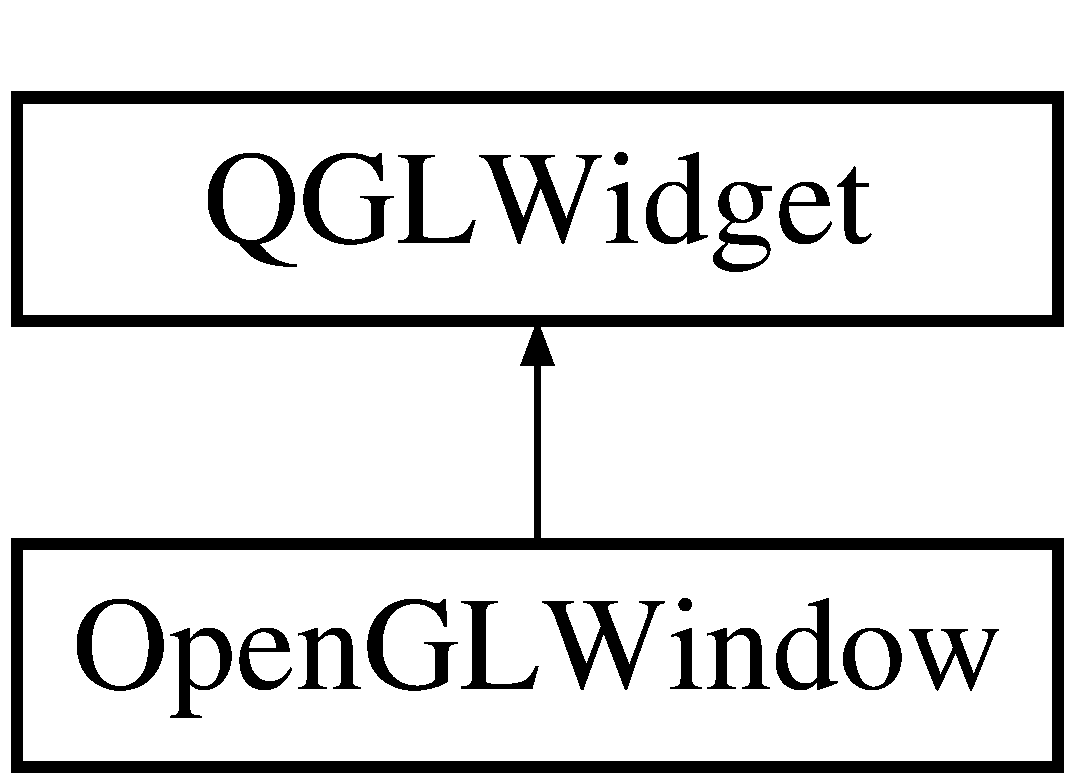
\includegraphics[height=2.000000cm]{class_d_o_1_1_open_g_l_window}
\end{center}
\end{figure}
\subsection*{Public Slots}
\begin{DoxyCompactItemize}
\item 
\hypertarget{class_d_o_1_1_open_g_l_window_a9dd55f307c18dfbdc8bc38918cb1cbb4}{void {\bfseries set\-Mesh} (const \hyperlink{group___draw3_d_ga4f1ab8c8365dc907bff111a6f87e6141}{Simple\-Triangle\-Mesh3f} \&mesh\-\_\-)}\label{class_d_o_1_1_open_g_l_window_a9dd55f307c18dfbdc8bc38918cb1cbb4}

\item 
\hypertarget{class_d_o_1_1_open_g_l_window_adae9e33c13a9e4b9d7fb847a29c8c199}{void {\bfseries display\-Mesh} ()}\label{class_d_o_1_1_open_g_l_window_adae9e33c13a9e4b9d7fb847a29c8c199}

\end{DoxyCompactItemize}
\subsection*{Signals}
\begin{DoxyCompactItemize}
\item 
\hypertarget{class_d_o_1_1_open_g_l_window_aa284cd282d9c672d56291f539ad864c7}{void {\bfseries moved\-Mouse} (int x, int \hyperlink{group___channel_accessors_gac90c52c5b3a7b2a7e3761e6e84f25778}{y}, Qt\-::\-Mouse\-Buttons buttons)}\label{class_d_o_1_1_open_g_l_window_aa284cd282d9c672d56291f539ad864c7}

\item 
\hypertarget{class_d_o_1_1_open_g_l_window_a211d59c0a6baf6072e762c542472efe6}{void {\bfseries pressed\-Mouse\-Buttons} (int x, int \hyperlink{group___channel_accessors_gac90c52c5b3a7b2a7e3761e6e84f25778}{y}, Qt\-::\-Mouse\-Buttons buttons)}\label{class_d_o_1_1_open_g_l_window_a211d59c0a6baf6072e762c542472efe6}

\item 
\hypertarget{class_d_o_1_1_open_g_l_window_aa6e288186f3b4d8668cbcb77d4d5cc71}{void {\bfseries released\-Mouse\-Buttons} (int x, int \hyperlink{group___channel_accessors_gac90c52c5b3a7b2a7e3761e6e84f25778}{y}, Qt\-::\-Mouse\-Buttons buttons)}\label{class_d_o_1_1_open_g_l_window_aa6e288186f3b4d8668cbcb77d4d5cc71}

\item 
\hypertarget{class_d_o_1_1_open_g_l_window_af3120a375a321654553779cf030a9508}{void {\bfseries pressed\-Key} (int key)}\label{class_d_o_1_1_open_g_l_window_af3120a375a321654553779cf030a9508}

\item 
\hypertarget{class_d_o_1_1_open_g_l_window_ac80bf1948c09a26181b72cb51f4ea4c3}{void {\bfseries released\-Key} (int key)}\label{class_d_o_1_1_open_g_l_window_ac80bf1948c09a26181b72cb51f4ea4c3}

\item 
\hypertarget{class_d_o_1_1_open_g_l_window_a497371cbad118b80dc07aa5c288f2573}{void {\bfseries send\-Event} (\hyperlink{struct_d_o_1_1_event}{Event} e)}\label{class_d_o_1_1_open_g_l_window_a497371cbad118b80dc07aa5c288f2573}

\end{DoxyCompactItemize}
\subsection*{Public Member Functions}
\begin{DoxyCompactItemize}
\item 
\hypertarget{class_d_o_1_1_open_g_l_window_a45e95ebd64819b9cda9828c60e38bb03}{{\bfseries Open\-G\-L\-Window} (int width, int height, const Q\-String \&window\-Title=\char`\"{}D\-O++\char`\"{}, int x=-\/1, int \hyperlink{group___channel_accessors_gac90c52c5b3a7b2a7e3761e6e84f25778}{y}=-\/1, Q\-Widget $\ast$parent=0)}\label{class_d_o_1_1_open_g_l_window_a45e95ebd64819b9cda9828c60e38bb03}

\end{DoxyCompactItemize}
\subsection*{Protected Member Functions}
\begin{DoxyCompactItemize}
\item 
\hypertarget{class_d_o_1_1_open_g_l_window_a2d3d45239c78255c23a70ca558b4d4f1}{void {\bfseries initialize\-G\-L} ()}\label{class_d_o_1_1_open_g_l_window_a2d3d45239c78255c23a70ca558b4d4f1}

\item 
\hypertarget{class_d_o_1_1_open_g_l_window_accfb24f32254fb98c049727597a53956}{void {\bfseries paint\-Event} (Q\-Paint\-Event $\ast$event)}\label{class_d_o_1_1_open_g_l_window_accfb24f32254fb98c049727597a53956}

\item 
\hypertarget{class_d_o_1_1_open_g_l_window_a3efe88f982dbec7825725dd954991139}{void {\bfseries resize\-G\-L} (int width, int height)}\label{class_d_o_1_1_open_g_l_window_a3efe88f982dbec7825725dd954991139}

\item 
\hypertarget{class_d_o_1_1_open_g_l_window_ad2272e344e46519f026cd02f419884f1}{void {\bfseries mouse\-Press\-Event} (Q\-Mouse\-Event $\ast$event)}\label{class_d_o_1_1_open_g_l_window_ad2272e344e46519f026cd02f419884f1}

\item 
\hypertarget{class_d_o_1_1_open_g_l_window_a35226f6549add1ff837c65888fcd00fc}{void {\bfseries mouse\-Release\-Event} (Q\-Mouse\-Event $\ast$event)}\label{class_d_o_1_1_open_g_l_window_a35226f6549add1ff837c65888fcd00fc}

\item 
\hypertarget{class_d_o_1_1_open_g_l_window_ae820c6a86f0a1908bf451f86db043489}{void {\bfseries mouse\-Move\-Event} (Q\-Mouse\-Event $\ast$event)}\label{class_d_o_1_1_open_g_l_window_ae820c6a86f0a1908bf451f86db043489}

\item 
\hypertarget{class_d_o_1_1_open_g_l_window_aca4aade13313c3deb599501abdd947f1}{void {\bfseries wheel\-Event} (Q\-Wheel\-Event $\ast$event)}\label{class_d_o_1_1_open_g_l_window_aca4aade13313c3deb599501abdd947f1}

\item 
\hypertarget{class_d_o_1_1_open_g_l_window_adf2e9d5e456a754a5459e8435b0b094b}{void {\bfseries key\-Press\-Event} (Q\-Key\-Event $\ast$event)}\label{class_d_o_1_1_open_g_l_window_adf2e9d5e456a754a5459e8435b0b094b}

\item 
\hypertarget{class_d_o_1_1_open_g_l_window_a9e0db194f0850420e6bf556d821e6080}{void {\bfseries key\-Release\-Event} (Q\-Key\-Event $\ast$event)}\label{class_d_o_1_1_open_g_l_window_a9e0db194f0850420e6bf556d821e6080}

\item 
\hypertarget{class_d_o_1_1_open_g_l_window_a5de2bd09256045c0b96e5a0be780fa85}{void {\bfseries close\-Event} (Q\-Close\-Event $\ast$event)}\label{class_d_o_1_1_open_g_l_window_a5de2bd09256045c0b96e5a0be780fa85}

\item 
\hypertarget{class_d_o_1_1_open_g_l_window_acfea3dd2775b4090eb0f33ec7be9c74f}{Q\-Point\-F {\bfseries normalize\-Pos} (const Q\-Point\-F \&local\-Pos) const }\label{class_d_o_1_1_open_g_l_window_acfea3dd2775b4090eb0f33ec7be9c74f}

\end{DoxyCompactItemize}


\subsection{Detailed Description}
Q\-G\-L\-Widget-\/derived class used to view 3\-D scenes. 

The documentation for this class was generated from the following file\-:\begin{DoxyCompactItemize}
\item 
src/\-D\-O/\-Graphics/\-Derived\-Q\-Objects/\hyperlink{_open_g_l_window_8hpp}{Open\-G\-L\-Window.\-hpp}\end{DoxyCompactItemize}

\hypertarget{class_d_o_1_1_painting_window}{\section{Painting\-Window Class Reference}
\label{class_d_o_1_1_painting_window}\index{Painting\-Window@{Painting\-Window}}
}


Q\-Widget-\/derived class on which we draw things. I choose not to use Q\-G\-L\-Widget because of some weird viewing artefacts... Maybe later...  




{\ttfamily \#include $<$Painting\-Window.\-hpp$>$}

Inheritance diagram for Painting\-Window\-:\begin{figure}[H]
\begin{center}
\leavevmode
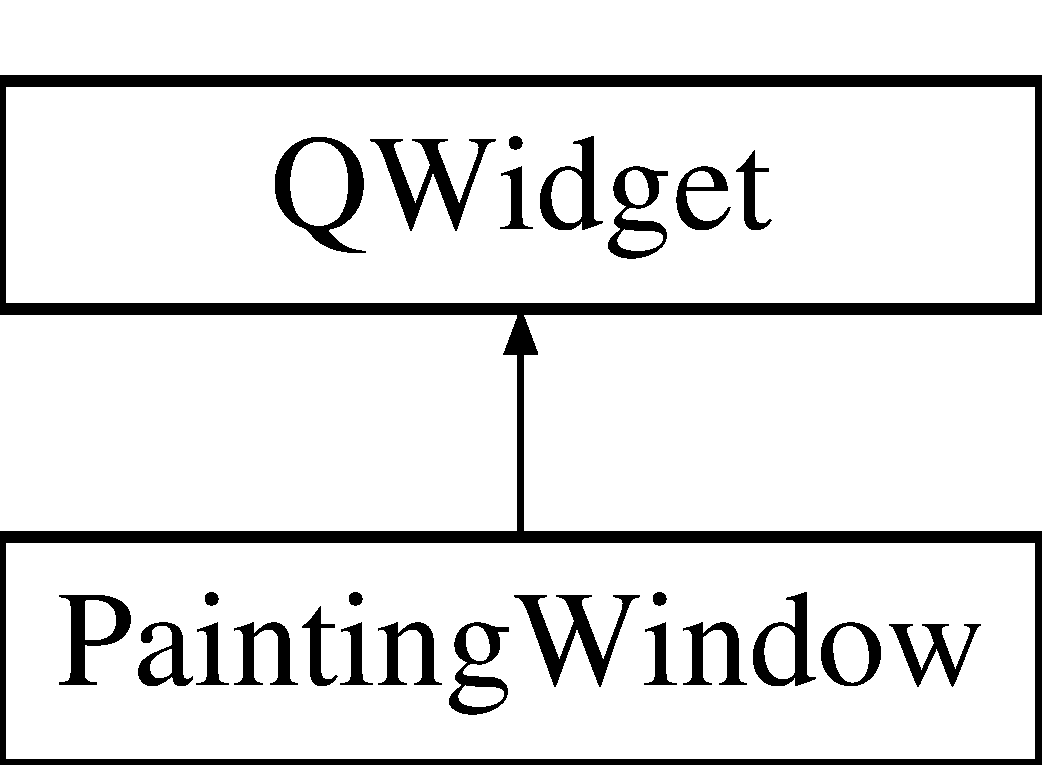
\includegraphics[height=2.000000cm]{class_d_o_1_1_painting_window}
\end{center}
\end{figure}
\subsection*{Public Slots}
\begin{DoxyCompactItemize}
\item 
\hypertarget{class_d_o_1_1_painting_window_a0d126d763b4c0a6250c9880354111ff4}{void {\bfseries draw\-Point} (int x, int \hyperlink{group___channel_accessors_gac90c52c5b3a7b2a7e3761e6e84f25778}{y}, const Q\-Color \&c)}\label{class_d_o_1_1_painting_window_a0d126d763b4c0a6250c9880354111ff4}

\item 
\hypertarget{class_d_o_1_1_painting_window_a1b8b8efe20acf5e73b7521b2a5a0d155}{void {\bfseries draw\-Point} (const Q\-Point\-F \&p, const Q\-Color \&c)}\label{class_d_o_1_1_painting_window_a1b8b8efe20acf5e73b7521b2a5a0d155}

\item 
\hypertarget{class_d_o_1_1_painting_window_a7051cc5fd5f19b9070b60e35dde2cdd9}{void {\bfseries draw\-Circle} (int xc, int yc, int r, const Q\-Color \&c, int pen\-Width=1)}\label{class_d_o_1_1_painting_window_a7051cc5fd5f19b9070b60e35dde2cdd9}

\item 
\hypertarget{class_d_o_1_1_painting_window_a3871290c78c7c8d13a6fb157dab84be2}{void {\bfseries draw\-Line} (int x1, int y1, int x2, int y2, const Q\-Color \&c, int pen\-Width=1)}\label{class_d_o_1_1_painting_window_a3871290c78c7c8d13a6fb157dab84be2}

\item 
\hypertarget{class_d_o_1_1_painting_window_a9a95ae8faa3b0064053ed5683c5aab19}{void {\bfseries draw\-Line} (const Q\-Point\-F \&p1, const Q\-Point\-F \&p2, const Q\-Color \&c, int pen\-Width=1)}\label{class_d_o_1_1_painting_window_a9a95ae8faa3b0064053ed5683c5aab19}

\item 
\hypertarget{class_d_o_1_1_painting_window_ab48b68294566b5ef4bce71a551a1a3fb}{void {\bfseries draw\-Ellipse} (int x, int \hyperlink{group___channel_accessors_gac90c52c5b3a7b2a7e3761e6e84f25778}{y}, int w, int h, const Q\-Color \&c, int pen\-Width=1)}\label{class_d_o_1_1_painting_window_ab48b68294566b5ef4bce71a551a1a3fb}

\item 
\hypertarget{class_d_o_1_1_painting_window_a5234523b6d222165c2ccd1dc1235bc71}{void {\bfseries draw\-Ellipse} (const Q\-Point\-F \&center, qreal r1, qreal r2, qreal degree, const Q\-Color \&c, int pen\-Width=1)}\label{class_d_o_1_1_painting_window_a5234523b6d222165c2ccd1dc1235bc71}

\item 
\hypertarget{class_d_o_1_1_painting_window_a0d31c2cf884bc801e677704a452fc092}{void {\bfseries draw\-Rect} (int x, int \hyperlink{group___channel_accessors_gac90c52c5b3a7b2a7e3761e6e84f25778}{y}, int w, int h, const Q\-Color \&c, int pen\-Width=1)}\label{class_d_o_1_1_painting_window_a0d31c2cf884bc801e677704a452fc092}

\item 
\hypertarget{class_d_o_1_1_painting_window_afa8643e3c75e788691af0971bbd78e04}{void {\bfseries draw\-Poly} (const Q\-Polygon\-F \&polygon, const Q\-Color \&c, int width)}\label{class_d_o_1_1_painting_window_afa8643e3c75e788691af0971bbd78e04}

\item 
\hypertarget{class_d_o_1_1_painting_window_a2d5d8b58859dce67f4d217ebb872a6ee}{void {\bfseries draw\-Text} (int x, int \hyperlink{group___channel_accessors_gac90c52c5b3a7b2a7e3761e6e84f25778}{y}, const Q\-String \&s, const Q\-Color \&c, int font\-Size, qreal \hyperlink{group___channel_accessors_gaa131549883a0aae99914ffe78da0dbcb}{alpha}, bool italic, bool bold, bool underline)}\label{class_d_o_1_1_painting_window_a2d5d8b58859dce67f4d217ebb872a6ee}

\item 
\hypertarget{class_d_o_1_1_painting_window_ab26208f9358949835cd0c2903a20010c}{void {\bfseries draw\-Arrow} (int a, int b, int c, int d, const Q\-Color \&col, int arrow\-Width, int arrow\-Height, int style, int width)}\label{class_d_o_1_1_painting_window_ab26208f9358949835cd0c2903a20010c}

\item 
\hypertarget{class_d_o_1_1_painting_window_a8a2b0d9ee239a064684d767e392f54f8}{void {\bfseries display} (const Q\-Image \&image, int xoff=0, int yoff=0, double fact=1.)}\label{class_d_o_1_1_painting_window_a8a2b0d9ee239a064684d767e392f54f8}

\item 
\hypertarget{class_d_o_1_1_painting_window_a8a255a3cbc57a58081502343b981e011}{void {\bfseries fill\-Circle} (int x, int \hyperlink{group___channel_accessors_gac90c52c5b3a7b2a7e3761e6e84f25778}{y}, int r, const Q\-Color \&c)}\label{class_d_o_1_1_painting_window_a8a255a3cbc57a58081502343b981e011}

\item 
\hypertarget{class_d_o_1_1_painting_window_af23f5a16098bd15457909bfad4cb6da0}{void {\bfseries fill\-Circle} (const Q\-Point\-F \&p, qreal r, const Q\-Color \&c)}\label{class_d_o_1_1_painting_window_af23f5a16098bd15457909bfad4cb6da0}

\item 
\hypertarget{class_d_o_1_1_painting_window_a049b71d8961d194ebedfb090ca58680b}{void {\bfseries fill\-Ellipse} (int x, int \hyperlink{group___channel_accessors_gac90c52c5b3a7b2a7e3761e6e84f25778}{y}, int w, int h, const Q\-Color \&c)}\label{class_d_o_1_1_painting_window_a049b71d8961d194ebedfb090ca58680b}

\item 
\hypertarget{class_d_o_1_1_painting_window_abae47f4f659a578a13cd6a68a4dd64ba}{void {\bfseries fill\-Ellipse} (const Q\-Point\-F \&p, qreal rx, qreal ry, qreal degree, const Q\-Color \&c)}\label{class_d_o_1_1_painting_window_abae47f4f659a578a13cd6a68a4dd64ba}

\item 
\hypertarget{class_d_o_1_1_painting_window_a3bd68bbe82c6c705bf58f9e86ae5702c}{void {\bfseries fill\-Poly} (const Q\-Polygon\-F \&polygon, const Q\-Color \&c)}\label{class_d_o_1_1_painting_window_a3bd68bbe82c6c705bf58f9e86ae5702c}

\item 
\hypertarget{class_d_o_1_1_painting_window_a11e314c190027a1c4bf11d24027dfbd4}{void {\bfseries fill\-Rect} (int x, int \hyperlink{group___channel_accessors_gac90c52c5b3a7b2a7e3761e6e84f25778}{y}, int w, int h, const Q\-Color \&c)}\label{class_d_o_1_1_painting_window_a11e314c190027a1c4bf11d24027dfbd4}

\item 
\hypertarget{class_d_o_1_1_painting_window_ac8bb3912a3ce86b15842e79d0b421204}{void {\bfseries clear} ()}\label{class_d_o_1_1_painting_window_ac8bb3912a3ce86b15842e79d0b421204}

\item 
\hypertarget{class_d_o_1_1_painting_window_a012338601cb5f258cb9e10a11c15afea}{void {\bfseries set\-Antialiasing} (bool on=true)}\label{class_d_o_1_1_painting_window_a012338601cb5f258cb9e10a11c15afea}

\item 
\hypertarget{class_d_o_1_1_painting_window_ae29eab5ad5147b234c346bb7e3dbd425}{void {\bfseries set\-Transparency} (bool on=true)}\label{class_d_o_1_1_painting_window_ae29eab5ad5147b234c346bb7e3dbd425}

\item 
\hypertarget{class_d_o_1_1_painting_window_a476ff5751c04f3a88e037b396638dcbe}{void {\bfseries save\-Screen} (const Q\-String \&filename)}\label{class_d_o_1_1_painting_window_a476ff5751c04f3a88e037b396638dcbe}

\item 
\hypertarget{class_d_o_1_1_painting_window_a0fbc37525f0506f77256b69d5009eccf}{void {\bfseries wait\-For\-Event} (int ms)}\label{class_d_o_1_1_painting_window_a0fbc37525f0506f77256b69d5009eccf}

\item 
\hypertarget{class_d_o_1_1_painting_window_a8ca6be03a1706b85ffe8389dde2b771f}{void {\bfseries event\-Listening\-Timer\-Stopped} ()}\label{class_d_o_1_1_painting_window_a8ca6be03a1706b85ffe8389dde2b771f}

\end{DoxyCompactItemize}
\subsection*{Signals}
\begin{DoxyCompactItemize}
\item 
\hypertarget{class_d_o_1_1_painting_window_aa284cd282d9c672d56291f539ad864c7}{void {\bfseries moved\-Mouse} (int x, int \hyperlink{group___channel_accessors_gac90c52c5b3a7b2a7e3761e6e84f25778}{y}, Qt\-::\-Mouse\-Buttons buttons)}\label{class_d_o_1_1_painting_window_aa284cd282d9c672d56291f539ad864c7}

\item 
\hypertarget{class_d_o_1_1_painting_window_a211d59c0a6baf6072e762c542472efe6}{void {\bfseries pressed\-Mouse\-Buttons} (int x, int \hyperlink{group___channel_accessors_gac90c52c5b3a7b2a7e3761e6e84f25778}{y}, Qt\-::\-Mouse\-Buttons buttons)}\label{class_d_o_1_1_painting_window_a211d59c0a6baf6072e762c542472efe6}

\item 
\hypertarget{class_d_o_1_1_painting_window_aa6e288186f3b4d8668cbcb77d4d5cc71}{void {\bfseries released\-Mouse\-Buttons} (int x, int \hyperlink{group___channel_accessors_gac90c52c5b3a7b2a7e3761e6e84f25778}{y}, Qt\-::\-Mouse\-Buttons buttons)}\label{class_d_o_1_1_painting_window_aa6e288186f3b4d8668cbcb77d4d5cc71}

\item 
\hypertarget{class_d_o_1_1_painting_window_af3120a375a321654553779cf030a9508}{void {\bfseries pressed\-Key} (int key)}\label{class_d_o_1_1_painting_window_af3120a375a321654553779cf030a9508}

\item 
\hypertarget{class_d_o_1_1_painting_window_ac80bf1948c09a26181b72cb51f4ea4c3}{void {\bfseries released\-Key} (int key)}\label{class_d_o_1_1_painting_window_ac80bf1948c09a26181b72cb51f4ea4c3}

\item 
\hypertarget{class_d_o_1_1_painting_window_a497371cbad118b80dc07aa5c288f2573}{void {\bfseries send\-Event} (\hyperlink{struct_d_o_1_1_event}{Event} e)}\label{class_d_o_1_1_painting_window_a497371cbad118b80dc07aa5c288f2573}

\end{DoxyCompactItemize}
\subsection*{Public Member Functions}
\begin{DoxyCompactItemize}
\item 
\hypertarget{class_d_o_1_1_painting_window_a7ea1bce9e0027f7fc48c1c138564d84c}{{\bfseries Painting\-Window} (int width, int height, const Q\-String \&window\-Title=\char`\"{}D\-O++\char`\"{}, int x=-\/1, int \hyperlink{group___channel_accessors_gac90c52c5b3a7b2a7e3761e6e84f25778}{y}=-\/1, Q\-Widget $\ast$parent=0)}\label{class_d_o_1_1_painting_window_a7ea1bce9e0027f7fc48c1c138564d84c}

\item 
\hypertarget{class_d_o_1_1_painting_window_ae1c14bcabfd3af8c71bb47964f7c5509}{Q\-Scroll\-Area $\ast$ {\bfseries scroll\-Area} ()}\label{class_d_o_1_1_painting_window_ae1c14bcabfd3af8c71bb47964f7c5509}

\end{DoxyCompactItemize}
\subsection*{Protected Member Functions}
\begin{DoxyCompactItemize}
\item 
\hypertarget{class_d_o_1_1_painting_window_ae820c6a86f0a1908bf451f86db043489}{void {\bfseries mouse\-Move\-Event} (Q\-Mouse\-Event $\ast$event)}\label{class_d_o_1_1_painting_window_ae820c6a86f0a1908bf451f86db043489}

\item 
\hypertarget{class_d_o_1_1_painting_window_ad2272e344e46519f026cd02f419884f1}{void {\bfseries mouse\-Press\-Event} (Q\-Mouse\-Event $\ast$event)}\label{class_d_o_1_1_painting_window_ad2272e344e46519f026cd02f419884f1}

\item 
\hypertarget{class_d_o_1_1_painting_window_a35226f6549add1ff837c65888fcd00fc}{void {\bfseries mouse\-Release\-Event} (Q\-Mouse\-Event $\ast$event)}\label{class_d_o_1_1_painting_window_a35226f6549add1ff837c65888fcd00fc}

\item 
\hypertarget{class_d_o_1_1_painting_window_adf2e9d5e456a754a5459e8435b0b094b}{void {\bfseries key\-Press\-Event} (Q\-Key\-Event $\ast$event)}\label{class_d_o_1_1_painting_window_adf2e9d5e456a754a5459e8435b0b094b}

\item 
\hypertarget{class_d_o_1_1_painting_window_a9e0db194f0850420e6bf556d821e6080}{void {\bfseries key\-Release\-Event} (Q\-Key\-Event $\ast$event)}\label{class_d_o_1_1_painting_window_a9e0db194f0850420e6bf556d821e6080}

\item 
\hypertarget{class_d_o_1_1_painting_window_accfb24f32254fb98c049727597a53956}{void {\bfseries paint\-Event} (Q\-Paint\-Event $\ast$event)}\label{class_d_o_1_1_painting_window_accfb24f32254fb98c049727597a53956}

\end{DoxyCompactItemize}


\subsection{Detailed Description}
Q\-Widget-\/derived class on which we draw things. I choose not to use Q\-G\-L\-Widget because of some weird viewing artefacts... Maybe later... 

The documentation for this class was generated from the following file\-:\begin{DoxyCompactItemize}
\item 
src/\-D\-O/\-Graphics/\-Derived\-Q\-Objects/\hyperlink{_painting_window_8hpp}{Painting\-Window.\-hpp}\end{DoxyCompactItemize}

\hypertarget{class_d_o_1_1_pixmap_item}{\section{Pixmap\-Item Class Reference}
\label{class_d_o_1_1_pixmap_item}\index{Pixmap\-Item@{Pixmap\-Item}}
}
Inheritance diagram for Pixmap\-Item\-:\begin{figure}[H]
\begin{center}
\leavevmode
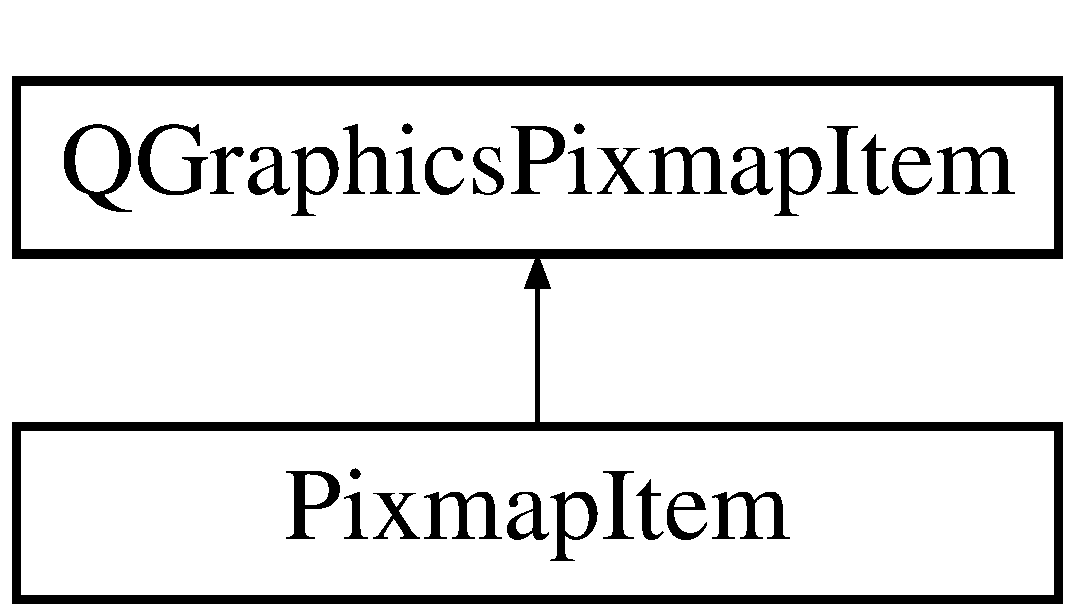
\includegraphics[height=2.000000cm]{class_d_o_1_1_pixmap_item}
\end{center}
\end{figure}
\subsection*{Public Member Functions}
\begin{DoxyCompactItemize}
\item 
\hypertarget{class_d_o_1_1_pixmap_item_a998f8cd639af4f18afab0219a0bfb0ec}{{\bfseries Pixmap\-Item} (Q\-Graphics\-Item $\ast$parent=0)}\label{class_d_o_1_1_pixmap_item_a998f8cd639af4f18afab0219a0bfb0ec}

\item 
\hypertarget{class_d_o_1_1_pixmap_item_a7dbbbb0c63ba52709ff0b73410093f8f}{{\bfseries Pixmap\-Item} (const Q\-Pixmap \&pixmap, Q\-Graphics\-Item $\ast$parent=0)}\label{class_d_o_1_1_pixmap_item_a7dbbbb0c63ba52709ff0b73410093f8f}

\end{DoxyCompactItemize}
\subsection*{Protected Member Functions}
\begin{DoxyCompactItemize}
\item 
\hypertarget{class_d_o_1_1_pixmap_item_adf2e9d5e456a754a5459e8435b0b094b}{void {\bfseries key\-Press\-Event} (Q\-Key\-Event $\ast$event)}\label{class_d_o_1_1_pixmap_item_adf2e9d5e456a754a5459e8435b0b094b}

\end{DoxyCompactItemize}


The documentation for this class was generated from the following file\-:\begin{DoxyCompactItemize}
\item 
src/\-D\-O/\-Graphics/\-Derived\-Q\-Objects/Pixmap\-Item.\-hpp\end{DoxyCompactItemize}

\hypertarget{struct_d_o_1_1_r}{\section{R Struct Reference}
\label{struct_d_o_1_1_r}\index{R@{R}}
}


Red channel name (R\-G\-B, R\-G\-B\-A).  




{\ttfamily \#include $<$Color.\-hpp$>$}



\subsection{Detailed Description}
Red channel name (R\-G\-B, R\-G\-B\-A). 

The documentation for this struct was generated from the following file\-:\begin{DoxyCompactItemize}
\item 
src/\-D\-O/\-Core/\hyperlink{_color_8hpp}{Color.\-hpp}\end{DoxyCompactItemize}

\hypertarget{class_d_o_1_1_range_iterator}{\section{Range\-Iterator$<$ N $>$ Class Template Reference}
\label{class_d_o_1_1_range_iterator}\index{Range\-Iterator$<$ N $>$@{Range\-Iterator$<$ N $>$}}
}


Range iterator class for N-\/dimensional array.  




{\ttfamily \#include $<$Locator.\-hpp$>$}

Inheritance diagram for Range\-Iterator$<$ N $>$\-:\begin{figure}[H]
\begin{center}
\leavevmode
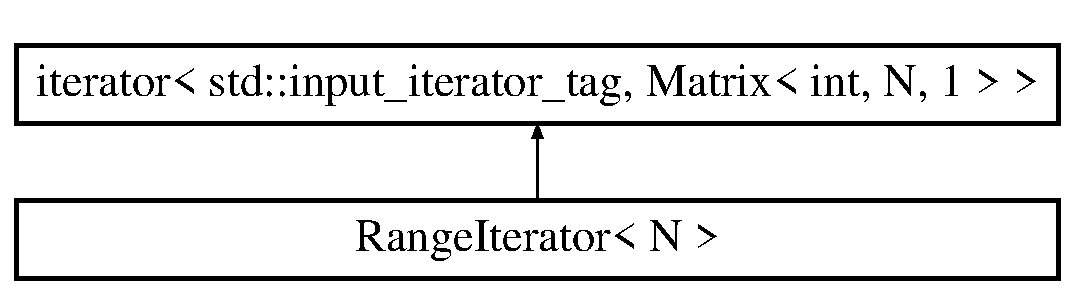
\includegraphics[height=2.000000cm]{class_d_o_1_1_range_iterator}
\end{center}
\end{figure}
\subsection*{Public Types}
\begin{DoxyCompactItemize}
\item 
\hypertarget{class_d_o_1_1_range_iterator_ac7678145ef96277c34f6516df859937c}{typedef \hyperlink{class_d_o_1_1_range_iterator}{Range\-Iterator} {\bfseries self\-\_\-type}}\label{class_d_o_1_1_range_iterator_ac7678145ef96277c34f6516df859937c}

\item 
\hypertarget{class_d_o_1_1_range_iterator_ae4fb477425bbeb20329d300396ac2582}{typedef Matrix$<$ int, N, 1 $>$ {\bfseries coord\-\_\-type}}\label{class_d_o_1_1_range_iterator_ae4fb477425bbeb20329d300396ac2582}

\item 
\hypertarget{class_d_o_1_1_range_iterator_a354195d823689d8ace92cf1499462880}{typedef Matrix$<$ int, N, 1 $>$ {\bfseries Coords}}\label{class_d_o_1_1_range_iterator_a354195d823689d8ace92cf1499462880}

\end{DoxyCompactItemize}
\subsection*{Public Member Functions}
\begin{DoxyCompactItemize}
\item 
\hypertarget{class_d_o_1_1_range_iterator_ae6bedf04454e9beb6719f298360397f9}{{\bfseries Range\-Iterator} (const coord\-\_\-type \&a, const coord\-\_\-type \&b)}\label{class_d_o_1_1_range_iterator_ae6bedf04454e9beb6719f298360397f9}

\item 
\hypertarget{class_d_o_1_1_range_iterator_a1fd855adf73ce7fa606fe3fb25cb30f1}{\hyperlink{class_d_o_1_1_range_iterator}{Range\-Iterator} \& {\bfseries operator=} (const \hyperlink{class_d_o_1_1_range_iterator}{self\-\_\-type} \&it)}\label{class_d_o_1_1_range_iterator_a1fd855adf73ce7fa606fe3fb25cb30f1}

\item 
\hypertarget{class_d_o_1_1_range_iterator_a61a6dd6a1c1c7f9bbccd31da5fa254f8}{bool {\bfseries operator==} (const \hyperlink{class_d_o_1_1_range_iterator}{self\-\_\-type} \&it) const }\label{class_d_o_1_1_range_iterator_a61a6dd6a1c1c7f9bbccd31da5fa254f8}

\item 
\hypertarget{class_d_o_1_1_range_iterator_aa14a207f9b5edbfa2fd1c62bc7320b99}{bool {\bfseries operator!=} (const \hyperlink{class_d_o_1_1_range_iterator}{self\-\_\-type} \&it) const }\label{class_d_o_1_1_range_iterator_aa14a207f9b5edbfa2fd1c62bc7320b99}

\item 
\hypertarget{class_d_o_1_1_range_iterator_a68c6d6abdde9fef27d6a4f2904212559}{\hyperlink{class_d_o_1_1_range_iterator}{self\-\_\-type} \& {\bfseries operator++} ()}\label{class_d_o_1_1_range_iterator_a68c6d6abdde9fef27d6a4f2904212559}

\item 
\hypertarget{class_d_o_1_1_range_iterator_a39f7c37604fd9845ff487b36b6f88602}{\hyperlink{class_d_o_1_1_range_iterator}{self\-\_\-type} {\bfseries operator++} (int)}\label{class_d_o_1_1_range_iterator_a39f7c37604fd9845ff487b36b6f88602}

\item 
\hypertarget{class_d_o_1_1_range_iterator_ab8d2f6e21f55ecfb383d1d4fd2103b1e}{coord\-\_\-type {\bfseries operator$\ast$} () const }\label{class_d_o_1_1_range_iterator_ab8d2f6e21f55ecfb383d1d4fd2103b1e}

\item 
\hypertarget{class_d_o_1_1_range_iterator_a40f822f265cedaeb23c3d015e6629253}{const coord\-\_\-type $\ast$ {\bfseries operator-\/$>$} () const }\label{class_d_o_1_1_range_iterator_a40f822f265cedaeb23c3d015e6629253}

\end{DoxyCompactItemize}
\subsection*{Protected Attributes}
\begin{DoxyCompactItemize}
\item 
\hypertarget{class_d_o_1_1_range_iterator_a284f00bbffebe7c1c4dfb317312708b6}{coord\-\_\-type {\bfseries a\-\_\-}}\label{class_d_o_1_1_range_iterator_a284f00bbffebe7c1c4dfb317312708b6}

\item 
\hypertarget{class_d_o_1_1_range_iterator_a08f8d2c104cdd1d188ed6c12f1a01a83}{coord\-\_\-type {\bfseries b\-\_\-}}\label{class_d_o_1_1_range_iterator_a08f8d2c104cdd1d188ed6c12f1a01a83}

\item 
\hypertarget{class_d_o_1_1_range_iterator_a0eb23f46bbde2be398f3e8b639f4eb2f}{coord\-\_\-type {\bfseries pos\-\_\-}}\label{class_d_o_1_1_range_iterator_a0eb23f46bbde2be398f3e8b639f4eb2f}

\item 
\hypertarget{class_d_o_1_1_range_iterator_adc52b9a89f713950bde219e658905261}{bool {\bfseries stop\-\_\-}}\label{class_d_o_1_1_range_iterator_adc52b9a89f713950bde219e658905261}

\end{DoxyCompactItemize}


\subsection{Detailed Description}
\subsubsection*{template$<$int N$>$class D\-O\-::\-Range\-Iterator$<$ N $>$}

Range iterator class for N-\/dimensional array. 

The documentation for this class was generated from the following file\-:\begin{DoxyCompactItemize}
\item 
src/\-D\-O/\-Core/\hyperlink{_locator_8hpp}{Locator.\-hpp}\end{DoxyCompactItemize}

\hypertarget{struct_d_o_1_1_s}{\section{S Struct Reference}
\label{struct_d_o_1_1_s}\index{S@{S}}
}


Saturation channel name (H\-S\-V).  




{\ttfamily \#include $<$Color.\-hpp$>$}



\subsection{Detailed Description}
Saturation channel name (H\-S\-V). 

The documentation for this struct was generated from the following file\-:\begin{DoxyCompactItemize}
\item 
src/\-D\-O/\-Core/\hyperlink{_color_8hpp}{Color.\-hpp}\end{DoxyCompactItemize}

\hypertarget{class_d_o_1_1_scroll_area}{\section{Scroll\-Area Class Reference}
\label{class_d_o_1_1_scroll_area}\index{Scroll\-Area@{Scroll\-Area}}
}


Q\-Scroll\-Area-\/derived class on which we embed the \hyperlink{class_d_o_1_1_painting_window}{Painting\-Window} class in order to scroll the contents of the window properly.  




{\ttfamily \#include $<$Painting\-Window.\-hpp$>$}

Inheritance diagram for Scroll\-Area\-:\begin{figure}[H]
\begin{center}
\leavevmode
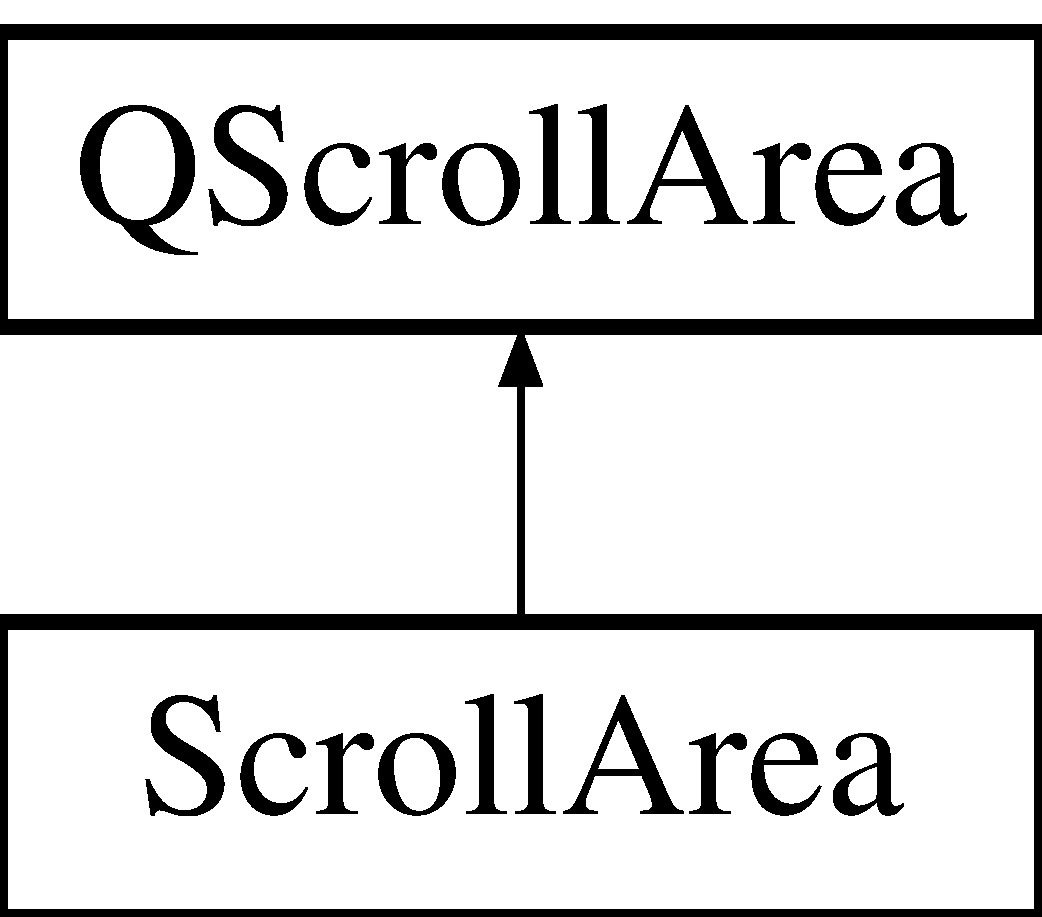
\includegraphics[height=2.000000cm]{class_d_o_1_1_scroll_area}
\end{center}
\end{figure}
\subsection*{Public Member Functions}
\begin{DoxyCompactItemize}
\item 
\hypertarget{class_d_o_1_1_scroll_area_a8a2de1733d4acfc45cd0bd449b882279}{{\bfseries Scroll\-Area} (Q\-Widget $\ast$parent=0)}\label{class_d_o_1_1_scroll_area_a8a2de1733d4acfc45cd0bd449b882279}

\end{DoxyCompactItemize}
\subsection*{Protected Member Functions}
\begin{DoxyCompactItemize}
\item 
\hypertarget{class_d_o_1_1_scroll_area_a5de2bd09256045c0b96e5a0be780fa85}{void {\bfseries close\-Event} (Q\-Close\-Event $\ast$event)}\label{class_d_o_1_1_scroll_area_a5de2bd09256045c0b96e5a0be780fa85}

\end{DoxyCompactItemize}


\subsection{Detailed Description}
Q\-Scroll\-Area-\/derived class on which we embed the \hyperlink{class_d_o_1_1_painting_window}{Painting\-Window} class in order to scroll the contents of the window properly. 

The documentation for this class was generated from the following file\-:\begin{DoxyCompactItemize}
\item 
src/\-D\-O/\-Graphics/\-Derived\-Q\-Objects/\hyperlink{_painting_window_8hpp}{Painting\-Window.\-hpp}\end{DoxyCompactItemize}

\hypertarget{class_d_o_1_1_simple_mesh}{\section{Simple\-Mesh$<$ Vector\-\_\-, Face\-\_\- $>$ Class Template Reference}
\label{class_d_o_1_1_simple_mesh}\index{Simple\-Mesh$<$ Vector\-\_\-, Face\-\_\- $>$@{Simple\-Mesh$<$ Vector\-\_\-, Face\-\_\- $>$}}
}


Simple mesh data structure.  




{\ttfamily \#include $<$Mesh.\-hpp$>$}

\subsection*{Public Types}
\begin{DoxyCompactItemize}
\item 
\hypertarget{class_d_o_1_1_simple_mesh_a4e0f748b614e44317e0961073fec8585}{typedef Vector\-\_\- {\bfseries Vector}}\label{class_d_o_1_1_simple_mesh_a4e0f748b614e44317e0961073fec8585}

\item 
\hypertarget{class_d_o_1_1_simple_mesh_aea0be5a8a64c17740c31d27605b844e1}{typedef Vector\-\_\- {\bfseries Point}}\label{class_d_o_1_1_simple_mesh_aea0be5a8a64c17740c31d27605b844e1}

\item 
\hypertarget{class_d_o_1_1_simple_mesh_aae4240566b5bfdaa1405339dd3831082}{typedef Face\-\_\- {\bfseries Face}}\label{class_d_o_1_1_simple_mesh_aae4240566b5bfdaa1405339dd3831082}

\end{DoxyCompactItemize}
\subsection*{Public Member Functions}
\begin{DoxyCompactItemize}
\item 
\hypertarget{class_d_o_1_1_simple_mesh_a4610f007d7ba928346ea0d9c80210b89}{std\-::vector$<$ Point $>$ \& {\bfseries vertices} ()}\label{class_d_o_1_1_simple_mesh_a4610f007d7ba928346ea0d9c80210b89}

\item 
\hypertarget{class_d_o_1_1_simple_mesh_a3313a9f1de5f63e9c74add9afb1f14ee}{std\-::vector$<$ Vector $>$ \& {\bfseries normals} ()}\label{class_d_o_1_1_simple_mesh_a3313a9f1de5f63e9c74add9afb1f14ee}

\item 
\hypertarget{class_d_o_1_1_simple_mesh_a4cc70785d08ebebc4df3e2d9cb603bfb}{std\-::vector$<$ Face $>$ \& {\bfseries faces} ()}\label{class_d_o_1_1_simple_mesh_a4cc70785d08ebebc4df3e2d9cb603bfb}

\item 
\hypertarget{class_d_o_1_1_simple_mesh_a87f418d4394ff3f5d938b001cdea64e3}{Point \& {\bfseries vertex} (size\-\_\-t i)}\label{class_d_o_1_1_simple_mesh_a87f418d4394ff3f5d938b001cdea64e3}

\item 
\hypertarget{class_d_o_1_1_simple_mesh_a83d364654c11d9af7b0b73872df412dc}{Vector \& {\bfseries normal} (size\-\_\-t i)}\label{class_d_o_1_1_simple_mesh_a83d364654c11d9af7b0b73872df412dc}

\item 
\hypertarget{class_d_o_1_1_simple_mesh_a08e3f8b85341fe7bd5f44a37a1734283}{Face \& {\bfseries face} (size\-\_\-t i)}\label{class_d_o_1_1_simple_mesh_a08e3f8b85341fe7bd5f44a37a1734283}

\item 
\hypertarget{class_d_o_1_1_simple_mesh_ae0a8f4e6ca684c4e43dc3dd18fcb5530}{Point \& {\bfseries vertex\-\_\-of\-\_\-face} (size\-\_\-t \hyperlink{group___channel_accessors_ga1dd2524c5b8d3db33137eedb803fc2ce}{v}, size\-\_\-t f)}\label{class_d_o_1_1_simple_mesh_ae0a8f4e6ca684c4e43dc3dd18fcb5530}

\item 
\hypertarget{class_d_o_1_1_simple_mesh_a1e445f3a0e3d6f411423af8ab8439dd5}{Vector \& {\bfseries normal\-\_\-of\-\_\-vertex\-\_\-of\-\_\-face} (size\-\_\-t \hyperlink{group___channel_accessors_ga1dd2524c5b8d3db33137eedb803fc2ce}{v}, size\-\_\-t f)}\label{class_d_o_1_1_simple_mesh_a1e445f3a0e3d6f411423af8ab8439dd5}

\item 
\hypertarget{class_d_o_1_1_simple_mesh_ab0c76900f50e7e713d0fe8f17e0e516d}{const std\-::vector$<$ Point $>$ \& {\bfseries vertices} () const }\label{class_d_o_1_1_simple_mesh_ab0c76900f50e7e713d0fe8f17e0e516d}

\item 
\hypertarget{class_d_o_1_1_simple_mesh_a03017e9adf738c62ee22ab8a87a84f0f}{const std\-::vector$<$ Vector $>$ \& {\bfseries normals} () const }\label{class_d_o_1_1_simple_mesh_a03017e9adf738c62ee22ab8a87a84f0f}

\item 
\hypertarget{class_d_o_1_1_simple_mesh_a5afef1c0c4baa6ef3d6ae8320167b6c8}{const std\-::vector$<$ Face $>$ \& {\bfseries faces} () const }\label{class_d_o_1_1_simple_mesh_a5afef1c0c4baa6ef3d6ae8320167b6c8}

\item 
\hypertarget{class_d_o_1_1_simple_mesh_a6a3138e4eae655177f255b17090602fd}{const Point \& {\bfseries vertex} (size\-\_\-t i) const }\label{class_d_o_1_1_simple_mesh_a6a3138e4eae655177f255b17090602fd}

\item 
\hypertarget{class_d_o_1_1_simple_mesh_a5c05a2740b7e83d17ce5eaa706ac8381}{const Vector \& {\bfseries normal} (size\-\_\-t i) const }\label{class_d_o_1_1_simple_mesh_a5c05a2740b7e83d17ce5eaa706ac8381}

\item 
\hypertarget{class_d_o_1_1_simple_mesh_afb365293bbdd726f291c685172d5522a}{const Face \& {\bfseries face} (size\-\_\-t i) const }\label{class_d_o_1_1_simple_mesh_afb365293bbdd726f291c685172d5522a}

\item 
\hypertarget{class_d_o_1_1_simple_mesh_addf2fb5edd942f095b116f11afa62618}{const Point \& {\bfseries vertex\-\_\-of\-\_\-face} (size\-\_\-t \hyperlink{group___channel_accessors_ga1dd2524c5b8d3db33137eedb803fc2ce}{v}, size\-\_\-t f) const }\label{class_d_o_1_1_simple_mesh_addf2fb5edd942f095b116f11afa62618}

\item 
\hypertarget{class_d_o_1_1_simple_mesh_ae5ff33ab9086c49c55d3fc85fcfc929f}{const Vector \& {\bfseries normal\-\_\-of\-\_\-vertex\-\_\-of\-\_\-face} (size\-\_\-t \hyperlink{group___channel_accessors_ga1dd2524c5b8d3db33137eedb803fc2ce}{v}, size\-\_\-t f) const }\label{class_d_o_1_1_simple_mesh_ae5ff33ab9086c49c55d3fc85fcfc929f}

\item 
\hypertarget{class_d_o_1_1_simple_mesh_a609e38971a439a95017a7ff40adc85af}{Point {\bfseries center} () const }\label{class_d_o_1_1_simple_mesh_a609e38971a439a95017a7ff40adc85af}

\item 
\hypertarget{class_d_o_1_1_simple_mesh_a2f18d56c763ffde4b8de9f9d4e00c20e}{Vector {\bfseries face\-\_\-normal} (size\-\_\-t f) const }\label{class_d_o_1_1_simple_mesh_a2f18d56c763ffde4b8de9f9d4e00c20e}

\end{DoxyCompactItemize}


\subsection{Detailed Description}
\subsubsection*{template$<$typename Vector\-\_\-, typename Face\-\_\-$>$class D\-O\-::\-Simple\-Mesh$<$ Vector\-\_\-, Face\-\_\- $>$}

Simple mesh data structure. 

The documentation for this class was generated from the following file\-:\begin{DoxyCompactItemize}
\item 
src/\-D\-O/\-Graphics/\hyperlink{_mesh_8hpp}{Mesh.\-hpp}\end{DoxyCompactItemize}

\hypertarget{class_d_o_1_1_sparse_multi_array}{\section{Sparse\-Multi\-Array$<$ T, N $>$ Class Template Reference}
\label{class_d_o_1_1_sparse_multi_array}\index{Sparse\-Multi\-Array$<$ T, N $>$@{Sparse\-Multi\-Array$<$ T, N $>$}}
}


Sparse N-\/dimensional array class.  




{\ttfamily \#include $<$Sparse\-Multi\-Array.\-hpp$>$}

\subsection*{Public Types}
\begin{DoxyCompactItemize}
\item 
\hypertarget{class_d_o_1_1_sparse_multi_array_ae4fb477425bbeb20329d300396ac2582}{typedef Matrix$<$ int, N, 1 $>$ \hyperlink{class_d_o_1_1_sparse_multi_array_ae4fb477425bbeb20329d300396ac2582}{coord\-\_\-type}}\label{class_d_o_1_1_sparse_multi_array_ae4fb477425bbeb20329d300396ac2582}

\begin{DoxyCompactList}\small\item\em S\-T\-L-\/like interface. \end{DoxyCompactList}\item 
\hypertarget{class_d_o_1_1_sparse_multi_array_a265a253612b46abed17c61b0a5e5ce30}{typedef T \hyperlink{class_d_o_1_1_sparse_multi_array_a265a253612b46abed17c61b0a5e5ce30}{value\-\_\-type}}\label{class_d_o_1_1_sparse_multi_array_a265a253612b46abed17c61b0a5e5ce30}

\begin{DoxyCompactList}\small\item\em S\-T\-L-\/like interface. \end{DoxyCompactList}\item 
\hypertarget{class_d_o_1_1_sparse_multi_array_ada51e68d31936547d3729c82daf6b7c6}{typedef unsigned int \hyperlink{class_d_o_1_1_sparse_multi_array_ada51e68d31936547d3729c82daf6b7c6}{size\-\_\-type}}\label{class_d_o_1_1_sparse_multi_array_ada51e68d31936547d3729c82daf6b7c6}

\begin{DoxyCompactList}\small\item\em S\-T\-L-\/like interface. \end{DoxyCompactList}\item 
\hypertarget{class_d_o_1_1_sparse_multi_array_aeb7d6a472fc07a6f5c9761e906c9f826}{typedef storage\-\_\-type\-::iterator \hyperlink{class_d_o_1_1_sparse_multi_array_aeb7d6a472fc07a6f5c9761e906c9f826}{iterator}}\label{class_d_o_1_1_sparse_multi_array_aeb7d6a472fc07a6f5c9761e906c9f826}

\begin{DoxyCompactList}\small\item\em iterator type. \end{DoxyCompactList}\item 
\hypertarget{class_d_o_1_1_sparse_multi_array_a136285f5e1620856973c0c4007453a57}{typedef \\*
storage\-\_\-type\-::const\-\_\-iterator \hyperlink{class_d_o_1_1_sparse_multi_array_a136285f5e1620856973c0c4007453a57}{const\-\_\-iterator}}\label{class_d_o_1_1_sparse_multi_array_a136285f5e1620856973c0c4007453a57}

\begin{DoxyCompactList}\small\item\em const\-\_\-iterator type. \end{DoxyCompactList}\item 
\hypertarget{class_d_o_1_1_sparse_multi_array_a8d8689998714f4431b104a5b21f43e9f}{typedef \\*
storage\-\_\-type\-::difference\-\_\-type \hyperlink{class_d_o_1_1_sparse_multi_array_a8d8689998714f4431b104a5b21f43e9f}{difference\-\_\-type}}\label{class_d_o_1_1_sparse_multi_array_a8d8689998714f4431b104a5b21f43e9f}

\begin{DoxyCompactList}\small\item\em difference\-\_\-type type. \end{DoxyCompactList}\item 
\hypertarget{class_d_o_1_1_sparse_multi_array_abe8933d436779a43cb5c1896ff5f2918}{typedef \hyperlink{class_d_o_1_1_sparse_multi_array_a265a253612b46abed17c61b0a5e5ce30}{value\-\_\-type} \& \hyperlink{class_d_o_1_1_sparse_multi_array_abe8933d436779a43cb5c1896ff5f2918}{reference}}\label{class_d_o_1_1_sparse_multi_array_abe8933d436779a43cb5c1896ff5f2918}

\begin{DoxyCompactList}\small\item\em reference type. \end{DoxyCompactList}\item 
\hypertarget{class_d_o_1_1_sparse_multi_array_afdb67657e63a66ed3fae7b0c9fd81b48}{typedef const \hyperlink{class_d_o_1_1_sparse_multi_array_a265a253612b46abed17c61b0a5e5ce30}{value\-\_\-type} \& \hyperlink{class_d_o_1_1_sparse_multi_array_afdb67657e63a66ed3fae7b0c9fd81b48}{const\-\_\-reference}}\label{class_d_o_1_1_sparse_multi_array_afdb67657e63a66ed3fae7b0c9fd81b48}

\begin{DoxyCompactList}\small\item\em const\-\_\-reference type. \end{DoxyCompactList}\end{DoxyCompactItemize}
\subsection*{Public Member Functions}
\begin{DoxyCompactItemize}
\item 
\hypertarget{class_d_o_1_1_sparse_multi_array_aa31288ffe2bcc901d1bea4ab9291c278}{\hyperlink{class_d_o_1_1_sparse_multi_array_aa31288ffe2bcc901d1bea4ab9291c278}{Sparse\-Multi\-Array} ()}\label{class_d_o_1_1_sparse_multi_array_aa31288ffe2bcc901d1bea4ab9291c278}

\begin{DoxyCompactList}\small\item\em Default constructor. \end{DoxyCompactList}\item 
\hypertarget{class_d_o_1_1_sparse_multi_array_adb2b3256fac8e82cdbb7532324788461}{\hyperlink{class_d_o_1_1_sparse_multi_array_adb2b3256fac8e82cdbb7532324788461}{Sparse\-Multi\-Array} (const \hyperlink{class_d_o_1_1_sparse_multi_array}{Sparse\-Multi\-Array} \&a)}\label{class_d_o_1_1_sparse_multi_array_adb2b3256fac8e82cdbb7532324788461}

\begin{DoxyCompactList}\small\item\em Copy constructor. \end{DoxyCompactList}\item 
\hypertarget{class_d_o_1_1_sparse_multi_array_ac6e61de369e994009e36f344f99c15ad}{bool \hyperlink{class_d_o_1_1_sparse_multi_array_ac6e61de369e994009e36f344f99c15ad}{empty} () const }\label{class_d_o_1_1_sparse_multi_array_ac6e61de369e994009e36f344f99c15ad}

\begin{DoxyCompactList}\small\item\em Checks if the sparse multi-\/array is empty. \end{DoxyCompactList}\item 
\hyperlink{class_d_o_1_1_sparse_multi_array_ae4fb477425bbeb20329d300396ac2582}{coord\-\_\-type} \hyperlink{class_d_o_1_1_sparse_multi_array_af74fcb5e1793fae740aa6cfa3da7b857}{min\-\_\-key} () const 
\item 
\hyperlink{class_d_o_1_1_sparse_multi_array_ae4fb477425bbeb20329d300396ac2582}{coord\-\_\-type} \hyperlink{class_d_o_1_1_sparse_multi_array_ad1a015f476d71c75dc93dadd5e344aec}{max\-\_\-key} () const 
\item 
\hypertarget{class_d_o_1_1_sparse_multi_array_a96c8baba4bb71887f51755f43047c026}{\hyperlink{class_d_o_1_1_sparse_multi_array_ae4fb477425bbeb20329d300396ac2582}{coord\-\_\-type} \hyperlink{class_d_o_1_1_sparse_multi_array_a96c8baba4bb71887f51755f43047c026}{all\-\_\-sizes} () const }\label{class_d_o_1_1_sparse_multi_array_a96c8baba4bb71887f51755f43047c026}

\begin{DoxyCompactList}\small\item\em Returns the theoretical capacity of the sparse multi-\/array. \end{DoxyCompactList}\item 
\hypertarget{class_d_o_1_1_sparse_multi_array_a64a533cf4dbc0310557c4a0c06ecef6a}{\hyperlink{class_d_o_1_1_sparse_multi_array_ae4fb477425bbeb20329d300396ac2582}{coord\-\_\-type} \hyperlink{class_d_o_1_1_sparse_multi_array_a64a533cf4dbc0310557c4a0c06ecef6a}{all\-\_\-actual\-\_\-sizes} () const }\label{class_d_o_1_1_sparse_multi_array_a64a533cf4dbc0310557c4a0c06ecef6a}

\begin{DoxyCompactList}\small\item\em Returns the actual N-\/dimensional size of the sparse multi-\/array. \end{DoxyCompactList}\item 
\hypertarget{class_d_o_1_1_sparse_multi_array_a503ab01f6c0142145d3434f6924714e7}{\hyperlink{class_d_o_1_1_sparse_multi_array_ada51e68d31936547d3729c82daf6b7c6}{size\-\_\-type} \hyperlink{class_d_o_1_1_sparse_multi_array_a503ab01f6c0142145d3434f6924714e7}{size} () const }\label{class_d_o_1_1_sparse_multi_array_a503ab01f6c0142145d3434f6924714e7}

\begin{DoxyCompactList}\small\item\em Returns the raw size of the storage data. \end{DoxyCompactList}\item 
\hypertarget{class_d_o_1_1_sparse_multi_array_a0ab5ce862c0331d9e45a6e1774fca131}{\hyperlink{class_d_o_1_1_sparse_multi_array_ada51e68d31936547d3729c82daf6b7c6}{size\-\_\-type} \hyperlink{class_d_o_1_1_sparse_multi_array_a0ab5ce862c0331d9e45a6e1774fca131}{max\-\_\-size} () const }\label{class_d_o_1_1_sparse_multi_array_a0ab5ce862c0331d9e45a6e1774fca131}

\begin{DoxyCompactList}\small\item\em Returns the capacity of the storage data. \end{DoxyCompactList}\item 
\hypertarget{class_d_o_1_1_sparse_multi_array_a475e9bb3f587819030146ed9b36a4fdd}{void \hyperlink{class_d_o_1_1_sparse_multi_array_a475e9bb3f587819030146ed9b36a4fdd}{swap} (\hyperlink{class_d_o_1_1_sparse_multi_array}{Sparse\-Multi\-Array} \&a)}\label{class_d_o_1_1_sparse_multi_array_a475e9bb3f587819030146ed9b36a4fdd}

\begin{DoxyCompactList}\small\item\em Efficient swapping of two 2\-D arrays. \end{DoxyCompactList}\item 
\hypertarget{class_d_o_1_1_sparse_multi_array_ac8bb3912a3ce86b15842e79d0b421204}{void \hyperlink{class_d_o_1_1_sparse_multi_array_ac8bb3912a3ce86b15842e79d0b421204}{clear} ()}\label{class_d_o_1_1_sparse_multi_array_ac8bb3912a3ce86b15842e79d0b421204}

\begin{DoxyCompactList}\small\item\em Erase all of the elements. \end{DoxyCompactList}\item 
\hypertarget{class_d_o_1_1_sparse_multi_array_a3a09e4b6b1d83553d805b190988e8e97}{\hyperlink{class_d_o_1_1_sparse_multi_array}{Sparse\-Multi\-Array} \& \hyperlink{class_d_o_1_1_sparse_multi_array_a3a09e4b6b1d83553d805b190988e8e97}{operator=} (const \hyperlink{class_d_o_1_1_sparse_multi_array}{Sparse\-Multi\-Array} \&a)}\label{class_d_o_1_1_sparse_multi_array_a3a09e4b6b1d83553d805b190988e8e97}

\begin{DoxyCompactList}\small\item\em Assignment operator. \end{DoxyCompactList}\item 
\hypertarget{class_d_o_1_1_sparse_multi_array_aaa3d8cf68eaa4f28a3320b36606d5e9d}{bool \hyperlink{class_d_o_1_1_sparse_multi_array_aaa3d8cf68eaa4f28a3320b36606d5e9d}{operator==} (const \hyperlink{class_d_o_1_1_sparse_multi_array}{Sparse\-Multi\-Array} \&a) const }\label{class_d_o_1_1_sparse_multi_array_aaa3d8cf68eaa4f28a3320b36606d5e9d}

\begin{DoxyCompactList}\small\item\em Equality operator. \end{DoxyCompactList}\item 
\hypertarget{class_d_o_1_1_sparse_multi_array_a5535cda5173e6de06f10f5d055142977}{bool \hyperlink{class_d_o_1_1_sparse_multi_array_a5535cda5173e6de06f10f5d055142977}{operator!=} (const \hyperlink{class_d_o_1_1_sparse_multi_array}{Sparse\-Multi\-Array} \&a) const }\label{class_d_o_1_1_sparse_multi_array_a5535cda5173e6de06f10f5d055142977}

\begin{DoxyCompactList}\small\item\em Inequality operator. \end{DoxyCompactList}\item 
\hypertarget{class_d_o_1_1_sparse_multi_array_a300969d60d0c092b583ae79889b3bd67}{\hyperlink{class_d_o_1_1_sparse_multi_array_a265a253612b46abed17c61b0a5e5ce30}{value\-\_\-type} \& \hyperlink{class_d_o_1_1_sparse_multi_array_a300969d60d0c092b583ae79889b3bd67}{operator\mbox{[}$\,$\mbox{]}} (const \hyperlink{class_d_o_1_1_sparse_multi_array_ae4fb477425bbeb20329d300396ac2582}{coord\-\_\-type} \&k)}\label{class_d_o_1_1_sparse_multi_array_a300969d60d0c092b583ae79889b3bd67}

\begin{DoxyCompactList}\small\item\em Mutable Access operator. \end{DoxyCompactList}\item 
\hypertarget{class_d_o_1_1_sparse_multi_array_a53e649bdfcb910262e552bbe9678c1dd}{const \hyperlink{class_d_o_1_1_sparse_multi_array_a265a253612b46abed17c61b0a5e5ce30}{value\-\_\-type} \& \hyperlink{class_d_o_1_1_sparse_multi_array_a53e649bdfcb910262e552bbe9678c1dd}{operator\mbox{[}$\,$\mbox{]}} (const \hyperlink{class_d_o_1_1_sparse_multi_array_ae4fb477425bbeb20329d300396ac2582}{coord\-\_\-type} \&k) const }\label{class_d_o_1_1_sparse_multi_array_a53e649bdfcb910262e552bbe9678c1dd}

\begin{DoxyCompactList}\small\item\em Constant access operator. \end{DoxyCompactList}\item 
\hypertarget{class_d_o_1_1_sparse_multi_array_ad69bd11391be1a1dba5c8202259664f8}{\hyperlink{class_d_o_1_1_sparse_multi_array_aeb7d6a472fc07a6f5c9761e906c9f826}{iterator} \hyperlink{class_d_o_1_1_sparse_multi_array_ad69bd11391be1a1dba5c8202259664f8}{begin} ()}\label{class_d_o_1_1_sparse_multi_array_ad69bd11391be1a1dba5c8202259664f8}

\begin{DoxyCompactList}\small\item\em Begin iterator. \end{DoxyCompactList}\item 
\hypertarget{class_d_o_1_1_sparse_multi_array_aa4b02d4f1a8500fb07a551069060709f}{\hyperlink{class_d_o_1_1_sparse_multi_array_a136285f5e1620856973c0c4007453a57}{const\-\_\-iterator} \hyperlink{class_d_o_1_1_sparse_multi_array_aa4b02d4f1a8500fb07a551069060709f}{begin} () const }\label{class_d_o_1_1_sparse_multi_array_aa4b02d4f1a8500fb07a551069060709f}

\begin{DoxyCompactList}\small\item\em Constant begin iterator. \end{DoxyCompactList}\item 
\hypertarget{class_d_o_1_1_sparse_multi_array_acad38d52497a975bfb6f2f6acd76631f}{\hyperlink{class_d_o_1_1_sparse_multi_array_aeb7d6a472fc07a6f5c9761e906c9f826}{iterator} \hyperlink{class_d_o_1_1_sparse_multi_array_acad38d52497a975bfb6f2f6acd76631f}{end} ()}\label{class_d_o_1_1_sparse_multi_array_acad38d52497a975bfb6f2f6acd76631f}

\begin{DoxyCompactList}\small\item\em End iterator. \end{DoxyCompactList}\item 
\hypertarget{class_d_o_1_1_sparse_multi_array_a350132543d80a1c1e5be844e6d2878ea}{\hyperlink{class_d_o_1_1_sparse_multi_array_a136285f5e1620856973c0c4007453a57}{const\-\_\-iterator} \hyperlink{class_d_o_1_1_sparse_multi_array_a350132543d80a1c1e5be844e6d2878ea}{end} () const }\label{class_d_o_1_1_sparse_multi_array_a350132543d80a1c1e5be844e6d2878ea}

\begin{DoxyCompactList}\small\item\em Constant end iterator. \end{DoxyCompactList}\end{DoxyCompactItemize}
\subsection*{Static Public Attributes}
\begin{DoxyCompactItemize}
\item 
\hypertarget{class_d_o_1_1_sparse_multi_array_a707c3ebff4b3587b5e3a4f8000ecb024}{static const \hyperlink{class_d_o_1_1_sparse_multi_array_ada51e68d31936547d3729c82daf6b7c6}{size\-\_\-type} \hyperlink{class_d_o_1_1_sparse_multi_array_a707c3ebff4b3587b5e3a4f8000ecb024}{dimension} = N}\label{class_d_o_1_1_sparse_multi_array_a707c3ebff4b3587b5e3a4f8000ecb024}

\begin{DoxyCompactList}\small\item\em Dimension. \end{DoxyCompactList}\end{DoxyCompactItemize}


\subsection{Detailed Description}
\subsubsection*{template$<$typename T, unsigned int N$>$class D\-O\-::\-Sparse\-Multi\-Array$<$ T, N $>$}

Sparse N-\/dimensional array class. 

\subsection{Member Function Documentation}
\hypertarget{class_d_o_1_1_sparse_multi_array_ad1a015f476d71c75dc93dadd5e344aec}{\index{D\-O\-::\-Sparse\-Multi\-Array@{D\-O\-::\-Sparse\-Multi\-Array}!max\-\_\-key@{max\-\_\-key}}
\index{max\-\_\-key@{max\-\_\-key}!DO::SparseMultiArray@{D\-O\-::\-Sparse\-Multi\-Array}}
\subsubsection[{max\-\_\-key}]{\setlength{\rightskip}{0pt plus 5cm}{\bf coord\-\_\-type} max\-\_\-key (
\begin{DoxyParamCaption}
{}
\end{DoxyParamCaption}
) const\hspace{0.3cm}{\ttfamily [inline]}}}\label{class_d_o_1_1_sparse_multi_array_ad1a015f476d71c75dc93dadd5e344aec}
Finds the maximum non-\/zero entry coordinates (in a lexicographical order). This function is computationally expensive. \hypertarget{class_d_o_1_1_sparse_multi_array_af74fcb5e1793fae740aa6cfa3da7b857}{\index{D\-O\-::\-Sparse\-Multi\-Array@{D\-O\-::\-Sparse\-Multi\-Array}!min\-\_\-key@{min\-\_\-key}}
\index{min\-\_\-key@{min\-\_\-key}!DO::SparseMultiArray@{D\-O\-::\-Sparse\-Multi\-Array}}
\subsubsection[{min\-\_\-key}]{\setlength{\rightskip}{0pt plus 5cm}{\bf coord\-\_\-type} min\-\_\-key (
\begin{DoxyParamCaption}
{}
\end{DoxyParamCaption}
) const\hspace{0.3cm}{\ttfamily [inline]}}}\label{class_d_o_1_1_sparse_multi_array_af74fcb5e1793fae740aa6cfa3da7b857}
Finds the minimum non-\/zero entry coordinates (in a lexicographical order). This function is computationally expensive. 

The documentation for this class was generated from the following file\-:\begin{DoxyCompactItemize}
\item 
src/\-D\-O/\-Core/\hyperlink{_sparse_multi_array_8hpp}{Sparse\-Multi\-Array.\-hpp}\end{DoxyCompactItemize}

\hypertarget{struct_d_o_1_1_meta_1_1_static_assertion}{\section{Static\-Assertion$<$ bool $>$ Struct Template Reference}
\label{struct_d_o_1_1_meta_1_1_static_assertion}\index{Static\-Assertion$<$ bool $>$@{Static\-Assertion$<$ bool $>$}}
}


Used for the implementation of D\-O\-\_\-\-S\-T\-A\-T\-I\-C\-\_\-\-A\-S\-S\-E\-R\-T.  




{\ttfamily \#include $<$Static\-Assert.\-hpp$>$}



\subsection{Detailed Description}
\subsubsection*{template$<$bool$>$struct D\-O\-::\-Meta\-::\-Static\-Assertion$<$ bool $>$}

Used for the implementation of D\-O\-\_\-\-S\-T\-A\-T\-I\-C\-\_\-\-A\-S\-S\-E\-R\-T. 

The documentation for this struct was generated from the following file\-:\begin{DoxyCompactItemize}
\item 
src/\-D\-O/\-Core/\hyperlink{_static_assert_8hpp}{Static\-Assert.\-hpp}\end{DoxyCompactItemize}

\hypertarget{struct_d_o_1_1_meta_1_1_static_assertion_3_01true_01_4}{\section{Static\-Assertion$<$ true $>$ Struct Template Reference}
\label{struct_d_o_1_1_meta_1_1_static_assertion_3_01true_01_4}\index{Static\-Assertion$<$ true $>$@{Static\-Assertion$<$ true $>$}}
}


Used for the implementation of D\-O\-\_\-\-S\-T\-A\-T\-I\-C\-\_\-\-A\-S\-S\-E\-R\-T.  




{\ttfamily \#include $<$Static\-Assert.\-hpp$>$}



\subsection{Detailed Description}
\subsubsection*{template$<$$>$struct D\-O\-::\-Meta\-::\-Static\-Assertion$<$ true $>$}

Used for the implementation of D\-O\-\_\-\-S\-T\-A\-T\-I\-C\-\_\-\-A\-S\-S\-E\-R\-T. 

The documentation for this struct was generated from the following file\-:\begin{DoxyCompactItemize}
\item 
src/\-D\-O/\-Core/\hyperlink{_static_assert_8hpp}{Static\-Assert.\-hpp}\end{DoxyCompactItemize}

\hypertarget{struct_d_o_1_1_meta_1_1_static_assertion_test}{\section{Static\-Assertion\-Test$<$ i $>$ Struct Template Reference}
\label{struct_d_o_1_1_meta_1_1_static_assertion_test}\index{Static\-Assertion\-Test$<$ i $>$@{Static\-Assertion\-Test$<$ i $>$}}
}


Used for the implementation of D\-O\-\_\-\-S\-T\-A\-T\-I\-C\-\_\-\-A\-S\-S\-E\-R\-T.  




{\ttfamily \#include $<$Static\-Assert.\-hpp$>$}



\subsection{Detailed Description}
\subsubsection*{template$<$int i$>$struct D\-O\-::\-Meta\-::\-Static\-Assertion\-Test$<$ i $>$}

Used for the implementation of D\-O\-\_\-\-S\-T\-A\-T\-I\-C\-\_\-\-A\-S\-S\-E\-R\-T. 

The documentation for this struct was generated from the following file\-:\begin{DoxyCompactItemize}
\item 
src/\-D\-O/\-Core/\hyperlink{_static_assert_8hpp}{Static\-Assert.\-hpp}\end{DoxyCompactItemize}

\hypertarget{class_d_o_1_1_timer}{\section{Timer Class Reference}
\label{class_d_o_1_1_timer}\index{Timer@{Timer}}
}


\hyperlink{class_d_o_1_1_timer}{Timer} class.  




{\ttfamily \#include $<$Timer.\-hpp$>$}

\subsection*{Public Member Functions}
\begin{DoxyCompactItemize}
\item 
\hypertarget{class_d_o_1_1_timer_a6a8bc5014802d569f6d01c4f36121a81}{\hyperlink{class_d_o_1_1_timer_a6a8bc5014802d569f6d01c4f36121a81}{Timer} ()}\label{class_d_o_1_1_timer_a6a8bc5014802d569f6d01c4f36121a81}

\begin{DoxyCompactList}\small\item\em Default constructor. \end{DoxyCompactList}\item 
\hypertarget{class_d_o_1_1_timer_a22ee094ca3f45aa4156b97d34fe678bf}{void \hyperlink{class_d_o_1_1_timer_a22ee094ca3f45aa4156b97d34fe678bf}{restart} ()}\label{class_d_o_1_1_timer_a22ee094ca3f45aa4156b97d34fe678bf}

\begin{DoxyCompactList}\small\item\em Reset the timer to zero. \end{DoxyCompactList}\item 
\hypertarget{class_d_o_1_1_timer_afb19d21ecfbd068a2f9c63ae52939df2}{double \hyperlink{class_d_o_1_1_timer_afb19d21ecfbd068a2f9c63ae52939df2}{elapsed} ()}\label{class_d_o_1_1_timer_afb19d21ecfbd068a2f9c63ae52939df2}

\begin{DoxyCompactList}\small\item\em Returns the elapsed time. \end{DoxyCompactList}\item 
\hypertarget{class_d_o_1_1_timer_a388f572c62279f839ee138a9afbdeeb5}{void \hyperlink{class_d_o_1_1_timer_a388f572c62279f839ee138a9afbdeeb5}{print} ()}\label{class_d_o_1_1_timer_a388f572c62279f839ee138a9afbdeeb5}

\begin{DoxyCompactList}\small\item\em Helper function that prints the elapsed time in a friendly manner. \end{DoxyCompactList}\end{DoxyCompactItemize}


\subsection{Detailed Description}
\hyperlink{class_d_o_1_1_timer}{Timer} class. 

The documentation for this class was generated from the following file\-:\begin{DoxyCompactItemize}
\item 
src/\-D\-O/\-Core/\hyperlink{_timer_8hpp}{Timer.\-hpp}\end{DoxyCompactItemize}

\hypertarget{class_d_o_1_1_track_ball}{\section{Track\-Ball Class Reference}
\label{class_d_o_1_1_track_ball}\index{Track\-Ball@{Track\-Ball}}
}


The \hyperlink{class_d_o_1_1_track_ball}{Track\-Ball} class is used the \hyperlink{class_d_o_1_1_open_g_l_window}{Open\-G\-L\-Window} class to allow the user to view the 3\-D scene interactively.  




{\ttfamily \#include $<$Open\-G\-L\-Window.\-hpp$>$}

\subsection*{Public Member Functions}
\begin{DoxyCompactItemize}
\item 
\hypertarget{class_d_o_1_1_track_ball_af48014ef141c7038209831db7ba1cb3c}{void {\bfseries push} (const Q\-Point\-F \&p, const Q\-Quaternion \&transformation)}\label{class_d_o_1_1_track_ball_af48014ef141c7038209831db7ba1cb3c}

\item 
\hypertarget{class_d_o_1_1_track_ball_a38def792dd690a4deb5d4dcd2900d8d4}{void {\bfseries move} (const Q\-Point\-F \&p, const Q\-Quaternion \&transformation)}\label{class_d_o_1_1_track_ball_a38def792dd690a4deb5d4dcd2900d8d4}

\item 
\hypertarget{class_d_o_1_1_track_ball_a7e815bb859d1468635bd6515581f083c}{void {\bfseries release} (const Q\-Point\-F \&p, const Q\-Quaternion \&transformation)}\label{class_d_o_1_1_track_ball_a7e815bb859d1468635bd6515581f083c}

\item 
\hypertarget{class_d_o_1_1_track_ball_aab269586dca28633e4a7adb4c580f00f}{Q\-Quaternion {\bfseries rotation} () const }\label{class_d_o_1_1_track_ball_aab269586dca28633e4a7adb4c580f00f}

\end{DoxyCompactItemize}


\subsection{Detailed Description}
The \hyperlink{class_d_o_1_1_track_ball}{Track\-Ball} class is used the \hyperlink{class_d_o_1_1_open_g_l_window}{Open\-G\-L\-Window} class to allow the user to view the 3\-D scene interactively. 

The documentation for this class was generated from the following file\-:\begin{DoxyCompactItemize}
\item 
src/\-D\-O/\-Graphics/\-Derived\-Q\-Objects/\hyperlink{_open_g_l_window_8hpp}{Open\-G\-L\-Window.\-hpp}\end{DoxyCompactItemize}

\hypertarget{class_d_o_1_1_tree}{\section{Tree$<$ T $>$ Class Template Reference}
\label{class_d_o_1_1_tree}\index{Tree$<$ T $>$@{Tree$<$ T $>$}}
}


The tree data structure is by definition an arborescence, in graph theory, i.\-e., an directed graph with a root vertex 'u' such that there is a unique path from 'u' to any vertex 'v' in the tree.  




{\ttfamily \#include $<$Tree.\-hpp$>$}

\subsection*{Public Types}
\begin{DoxyCompactItemize}
\item 
\hypertarget{class_d_o_1_1_tree_a265a253612b46abed17c61b0a5e5ce30}{typedef T {\bfseries value\-\_\-type}}\label{class_d_o_1_1_tree_a265a253612b46abed17c61b0a5e5ce30}

\item 
\hypertarget{class_d_o_1_1_tree_a680c78d51cff3fd301666dd75bdbe49d}{typedef T $\ast$ {\bfseries pointer}}\label{class_d_o_1_1_tree_a680c78d51cff3fd301666dd75bdbe49d}

\item 
\hypertarget{class_d_o_1_1_tree_a53d259f0075b22d7646e373816830e8e}{typedef const T $\ast$ {\bfseries const\-\_\-pointer}}\label{class_d_o_1_1_tree_a53d259f0075b22d7646e373816830e8e}

\item 
\hypertarget{class_d_o_1_1_tree_a9b1a63f171d76a7a3995b6858e99f2ea}{typedef T \& {\bfseries reference}}\label{class_d_o_1_1_tree_a9b1a63f171d76a7a3995b6858e99f2ea}

\item 
\hypertarget{class_d_o_1_1_tree_af9ba3e25df088c62f7d535b91672cda9}{typedef const T \& {\bfseries const\-\_\-reference}}\label{class_d_o_1_1_tree_af9ba3e25df088c62f7d535b91672cda9}

\item 
\hypertarget{class_d_o_1_1_tree_a957b4932a1fe961a3b2f9c3df003afa5}{typedef Node {\bfseries node\-\_\-type}}\label{class_d_o_1_1_tree_a957b4932a1fe961a3b2f9c3df003afa5}

\item 
\hypertarget{class_d_o_1_1_tree_a5aaef33bc2a4eadb7938c46e008ece74}{typedef Node\-Handle$<$ false $>$ {\bfseries node\-\_\-handle}}\label{class_d_o_1_1_tree_a5aaef33bc2a4eadb7938c46e008ece74}

\item 
\hypertarget{class_d_o_1_1_tree_a63679e305245efb895f61220fae8b308}{typedef Children\-Iterator$<$ false $>$ {\bfseries children\-\_\-iterator}}\label{class_d_o_1_1_tree_a63679e305245efb895f61220fae8b308}

\item 
\hypertarget{class_d_o_1_1_tree_a1b68ac2ad80415afa4ab778a852c4880}{typedef Depth\-First\-Iterator$<$ false $>$ {\bfseries depth\-\_\-first\-\_\-iterator}}\label{class_d_o_1_1_tree_a1b68ac2ad80415afa4ab778a852c4880}

\item 
\hypertarget{class_d_o_1_1_tree_ab0764299e60d2534fd17a0e72c3fb546}{typedef Breadth\-First\-Iterator\\*
$<$ false $>$ {\bfseries breadth\-\_\-first\-\_\-iterator}}\label{class_d_o_1_1_tree_ab0764299e60d2534fd17a0e72c3fb546}

\item 
\hypertarget{class_d_o_1_1_tree_adbbdf19f38b14d4da76d1614be080d00}{typedef Leaf\-Iterator$<$ false $>$ {\bfseries leaf\-\_\-iterator}}\label{class_d_o_1_1_tree_adbbdf19f38b14d4da76d1614be080d00}

\item 
\hypertarget{class_d_o_1_1_tree_ae753899577d159fa4affc363db9732fa}{typedef Node\-Handle$<$ true $>$ {\bfseries const\-\_\-node\-\_\-handle}}\label{class_d_o_1_1_tree_ae753899577d159fa4affc363db9732fa}

\item 
\hypertarget{class_d_o_1_1_tree_ae66bc4ac2dc4f6a2911f3c681a87edd6}{typedef Children\-Iterator$<$ true $>$ {\bfseries const\-\_\-children\-\_\-iterator}}\label{class_d_o_1_1_tree_ae66bc4ac2dc4f6a2911f3c681a87edd6}

\item 
\hypertarget{class_d_o_1_1_tree_a988b24ed2ea871f299c7b57b793d8284}{typedef Depth\-First\-Iterator$<$ true $>$ {\bfseries const\-\_\-depth\-\_\-first\-\_\-iterator}}\label{class_d_o_1_1_tree_a988b24ed2ea871f299c7b57b793d8284}

\item 
\hypertarget{class_d_o_1_1_tree_abf6d39fccb2d13ee71f1b66dbafbd851}{typedef Breadth\-First\-Iterator\\*
$<$ true $>$ {\bfseries const\-\_\-breadth\-\_\-first\-\_\-iterator}}\label{class_d_o_1_1_tree_abf6d39fccb2d13ee71f1b66dbafbd851}

\item 
\hypertarget{class_d_o_1_1_tree_a61229ff3e7defea14d8fb68f94cc9ae6}{typedef Leaf\-Iterator$<$ true $>$ {\bfseries const\-\_\-leaf\-\_\-iterator}}\label{class_d_o_1_1_tree_a61229ff3e7defea14d8fb68f94cc9ae6}

\end{DoxyCompactItemize}
\subsection*{Public Member Functions}
\begin{DoxyCompactItemize}
\item 
\hypertarget{class_d_o_1_1_tree_a3dee5770ede29888f2c0136bbd7f5a95}{\hyperlink{class_d_o_1_1_tree_a3dee5770ede29888f2c0136bbd7f5a95}{Tree} ()}\label{class_d_o_1_1_tree_a3dee5770ede29888f2c0136bbd7f5a95}

\begin{DoxyCompactList}\small\item\em Default constructor. \end{DoxyCompactList}\item 
\hypertarget{class_d_o_1_1_tree_ab2eeead563db79ec963561503f3db441}{\hyperlink{class_d_o_1_1_tree_ab2eeead563db79ec963561503f3db441}{Tree} (const T \&\hyperlink{group___channel_accessors_ga1dd2524c5b8d3db33137eedb803fc2ce}{v})}\label{class_d_o_1_1_tree_ab2eeead563db79ec963561503f3db441}

\begin{DoxyCompactList}\small\item\em Constructor with root vertex. \end{DoxyCompactList}\item 
\hypertarget{class_d_o_1_1_tree_a9603ba799d51fe7b2e8d2ac78abfa535}{\hyperlink{class_d_o_1_1_tree_a9603ba799d51fe7b2e8d2ac78abfa535}{Tree} (const \hyperlink{class_d_o_1_1_tree}{Tree} \&t)}\label{class_d_o_1_1_tree_a9603ba799d51fe7b2e8d2ac78abfa535}

\begin{DoxyCompactList}\small\item\em Copy constructor. \end{DoxyCompactList}\item 
\hypertarget{class_d_o_1_1_tree_a4d2d4eaa9ac9d347549728060df29842}{\hyperlink{class_d_o_1_1_tree_a4d2d4eaa9ac9d347549728060df29842}{$\sim$\-Tree} ()}\label{class_d_o_1_1_tree_a4d2d4eaa9ac9d347549728060df29842}

\begin{DoxyCompactList}\small\item\em Destructor. \end{DoxyCompactList}\item 
\hypertarget{class_d_o_1_1_tree_a54e71c610e133a9fb85c1b156d94da42}{\hyperlink{class_d_o_1_1_tree}{Tree} \& \hyperlink{class_d_o_1_1_tree_a54e71c610e133a9fb85c1b156d94da42}{operator=} (const \hyperlink{class_d_o_1_1_tree}{Tree} \&t)}\label{class_d_o_1_1_tree_a54e71c610e133a9fb85c1b156d94da42}

\begin{DoxyCompactList}\small\item\em Assignment operator. \end{DoxyCompactList}\item 
bool \hyperlink{class_d_o_1_1_tree_a72e422ad913c00d5443bfe02530394a1}{operator!=} (const \hyperlink{class_d_o_1_1_tree}{Tree} \&t) const 
\begin{DoxyCompactList}\small\item\em Equality operator. \end{DoxyCompactList}\item 
\hypertarget{class_d_o_1_1_tree_a4ef88b6304d9d660dece87018d740033}{void \hyperlink{class_d_o_1_1_tree_a4ef88b6304d9d660dece87018d740033}{swap} (const \hyperlink{class_d_o_1_1_tree}{Tree} \&t)}\label{class_d_o_1_1_tree_a4ef88b6304d9d660dece87018d740033}

\begin{DoxyCompactList}\small\item\em Swap function. \end{DoxyCompactList}\item 
\hypertarget{class_d_o_1_1_tree_ac8bb3912a3ce86b15842e79d0b421204}{void \hyperlink{class_d_o_1_1_tree_ac8bb3912a3ce86b15842e79d0b421204}{clear} ()}\label{class_d_o_1_1_tree_ac8bb3912a3ce86b15842e79d0b421204}

\begin{DoxyCompactList}\small\item\em Clear function. \end{DoxyCompactList}\item 
\hypertarget{class_d_o_1_1_tree_ac6e61de369e994009e36f344f99c15ad}{bool \hyperlink{class_d_o_1_1_tree_ac6e61de369e994009e36f344f99c15ad}{empty} () const }\label{class_d_o_1_1_tree_ac6e61de369e994009e36f344f99c15ad}

\begin{DoxyCompactList}\small\item\em Returns if the tree is empty. \end{DoxyCompactList}\item 
\hypertarget{class_d_o_1_1_tree_a37a865cf4e8665ad843cbd3fa7fac805}{void \hyperlink{class_d_o_1_1_tree_a37a865cf4e8665ad843cbd3fa7fac805}{set\-\_\-root} (const T \&\hyperlink{group___channel_accessors_ga1dd2524c5b8d3db33137eedb803fc2ce}{v})}\label{class_d_o_1_1_tree_a37a865cf4e8665ad843cbd3fa7fac805}

\begin{DoxyCompactList}\small\item\em Set the root of the tree with value 'v'. \end{DoxyCompactList}\item 
node\-\_\-handle \hyperlink{class_d_o_1_1_tree_a3b85d61d075fcee2959be9c1b564e23b}{insert\-\_\-sibling\-\_\-before} (node\-\_\-handle n, const T \&\hyperlink{group___channel_accessors_ga1dd2524c5b8d3db33137eedb803fc2ce}{v})
\item 
node\-\_\-handle \hyperlink{class_d_o_1_1_tree_abe4588e8f434f4ab6fa9654427cc4dda}{insert\-\_\-sibling\-\_\-after} (node\-\_\-handle n, const T \&\hyperlink{group___channel_accessors_ga1dd2524c5b8d3db33137eedb803fc2ce}{v})
\item 
\hypertarget{class_d_o_1_1_tree_a120c2a2f64f45604e96c85ca3984aaed}{node\-\_\-handle \hyperlink{class_d_o_1_1_tree_a120c2a2f64f45604e96c85ca3984aaed}{append\-\_\-child} (node\-\_\-handle n, const T \&\hyperlink{group___channel_accessors_ga1dd2524c5b8d3db33137eedb803fc2ce}{v})}\label{class_d_o_1_1_tree_a120c2a2f64f45604e96c85ca3984aaed}

\begin{DoxyCompactList}\small\item\em Append child to specified node and returns the child node handle. \end{DoxyCompactList}\item 
\hypertarget{class_d_o_1_1_tree_aa3b8256209a0a013e04a479b0ed5d0a6}{node\-\_\-handle \hyperlink{class_d_o_1_1_tree_aa3b8256209a0a013e04a479b0ed5d0a6}{prepend\-\_\-child} (node\-\_\-handle n, const T \&\hyperlink{group___channel_accessors_ga1dd2524c5b8d3db33137eedb803fc2ce}{v})}\label{class_d_o_1_1_tree_aa3b8256209a0a013e04a479b0ed5d0a6}

\begin{DoxyCompactList}\small\item\em Prepend child to specified node. \end{DoxyCompactList}\item 
\hypertarget{class_d_o_1_1_tree_a15908e24c5d1f66b6d96b548291ff5c3}{void \hyperlink{class_d_o_1_1_tree_a15908e24c5d1f66b6d96b548291ff5c3}{append\-\_\-child\-\_\-tree} (node\-\_\-handle node, \hyperlink{class_d_o_1_1_tree}{Tree} \&tree)}\label{class_d_o_1_1_tree_a15908e24c5d1f66b6d96b548291ff5c3}

\begin{DoxyCompactList}\small\item\em Append child tree to specified node. \end{DoxyCompactList}\item 
\hypertarget{class_d_o_1_1_tree_a4261f34846d379bad5deee88b905762f}{void \hyperlink{class_d_o_1_1_tree_a4261f34846d379bad5deee88b905762f}{prepend\-\_\-child\-\_\-tree} (node\-\_\-handle node, \hyperlink{class_d_o_1_1_tree}{Tree} \&tree)}\label{class_d_o_1_1_tree_a4261f34846d379bad5deee88b905762f}

\begin{DoxyCompactList}\small\item\em Prepend child tree to specified node. \end{DoxyCompactList}\item 
\hyperlink{class_d_o_1_1_tree}{Tree} \hyperlink{class_d_o_1_1_tree_aba6ece339051b6bad21840d986bd0a3a}{cut\-\_\-tree} (node\-\_\-handle node)
\item 
void \hyperlink{class_d_o_1_1_tree_a73a3166a18f4d9091d128d7ede38d740}{delete\-\_\-subtree} (node\-\_\-handle node)
\item 
\hypertarget{class_d_o_1_1_tree_acebef34190c5b61c05d2c5e9308c00a4}{node\-\_\-handle \hyperlink{class_d_o_1_1_tree_acebef34190c5b61c05d2c5e9308c00a4}{begin} ()}\label{class_d_o_1_1_tree_acebef34190c5b61c05d2c5e9308c00a4}

\begin{DoxyCompactList}\small\item\em Returns the root of the tree. \end{DoxyCompactList}\item 
\hypertarget{class_d_o_1_1_tree_a84c3a10b394fa5d0687d032a086c3e96}{node\-\_\-handle \hyperlink{class_d_o_1_1_tree_a84c3a10b394fa5d0687d032a086c3e96}{end} ()}\label{class_d_o_1_1_tree_a84c3a10b394fa5d0687d032a086c3e96}

\begin{DoxyCompactList}\small\item\em Returns the last node of the tree. \end{DoxyCompactList}\item 
\hypertarget{class_d_o_1_1_tree_a50e15fc2193067f33398e37e01d8a2ae}{node\-\_\-handle \hyperlink{class_d_o_1_1_tree_a50e15fc2193067f33398e37e01d8a2ae}{parent\-\_\-of} (node\-\_\-handle \hyperlink{group___channel_accessors_ga1dd2524c5b8d3db33137eedb803fc2ce}{v})}\label{class_d_o_1_1_tree_a50e15fc2193067f33398e37e01d8a2ae}

\begin{DoxyCompactList}\small\item\em Returns the parent of the input node. \end{DoxyCompactList}\item 
\hypertarget{class_d_o_1_1_tree_ae25e673000362d17c5dbe34e13ed26a9}{children\-\_\-iterator \hyperlink{class_d_o_1_1_tree_ae25e673000362d17c5dbe34e13ed26a9}{children\-\_\-begin} (node\-\_\-handle \hyperlink{group___channel_accessors_ga1dd2524c5b8d3db33137eedb803fc2ce}{v})}\label{class_d_o_1_1_tree_ae25e673000362d17c5dbe34e13ed26a9}

\begin{DoxyCompactList}\small\item\em Returns the first child iterator. \end{DoxyCompactList}\item 
\hypertarget{class_d_o_1_1_tree_a4bbe761f0929f34567f339615d616bda}{children\-\_\-iterator \hyperlink{class_d_o_1_1_tree_a4bbe761f0929f34567f339615d616bda}{children\-\_\-end} ()}\label{class_d_o_1_1_tree_a4bbe761f0929f34567f339615d616bda}

\begin{DoxyCompactList}\small\item\em Returns the last child iterator. \end{DoxyCompactList}\item 
\hypertarget{class_d_o_1_1_tree_aacea50afcacf312bf2254b5c6aa515d4}{depth\-\_\-first\-\_\-iterator \hyperlink{class_d_o_1_1_tree_aacea50afcacf312bf2254b5c6aa515d4}{depth\-\_\-first\-\_\-begin} ()}\label{class_d_o_1_1_tree_aacea50afcacf312bf2254b5c6aa515d4}

\begin{DoxyCompactList}\small\item\em Returns the first depth-\/first iterator. \end{DoxyCompactList}\item 
\hypertarget{class_d_o_1_1_tree_ab20dfe0da9bfd5b4e021b4081813555f}{depth\-\_\-first\-\_\-iterator \hyperlink{class_d_o_1_1_tree_ab20dfe0da9bfd5b4e021b4081813555f}{depth\-\_\-first\-\_\-end} ()}\label{class_d_o_1_1_tree_ab20dfe0da9bfd5b4e021b4081813555f}

\begin{DoxyCompactList}\small\item\em Returns the last depth-\/first iterator. \end{DoxyCompactList}\item 
\hypertarget{class_d_o_1_1_tree_aeff3d8457fe71b935b10ce476917928b}{breadth\-\_\-first\-\_\-iterator \hyperlink{class_d_o_1_1_tree_aeff3d8457fe71b935b10ce476917928b}{breadth\-\_\-first\-\_\-begin} ()}\label{class_d_o_1_1_tree_aeff3d8457fe71b935b10ce476917928b}

\begin{DoxyCompactList}\small\item\em Returns the first breadth-\/first iterator. \end{DoxyCompactList}\item 
\hypertarget{class_d_o_1_1_tree_a96a5a047c112cbba0d54d746a6073499}{breadth\-\_\-first\-\_\-iterator \hyperlink{class_d_o_1_1_tree_a96a5a047c112cbba0d54d746a6073499}{breadth\-\_\-first\-\_\-end} ()}\label{class_d_o_1_1_tree_a96a5a047c112cbba0d54d746a6073499}

\begin{DoxyCompactList}\small\item\em Returns the last breadth-\/first iterator. \end{DoxyCompactList}\item 
\hypertarget{class_d_o_1_1_tree_a3cc80a426bf788cd6c5b94d2084b69cb}{leaf\-\_\-iterator \hyperlink{class_d_o_1_1_tree_a3cc80a426bf788cd6c5b94d2084b69cb}{leaf\-\_\-begin} ()}\label{class_d_o_1_1_tree_a3cc80a426bf788cd6c5b94d2084b69cb}

\begin{DoxyCompactList}\small\item\em Returns the first leaf iterator. \end{DoxyCompactList}\item 
\hypertarget{class_d_o_1_1_tree_ac8e0c3fa6a007feaa01c7c18d314d145}{leaf\-\_\-iterator \hyperlink{class_d_o_1_1_tree_ac8e0c3fa6a007feaa01c7c18d314d145}{leaf\-\_\-end} ()}\label{class_d_o_1_1_tree_ac8e0c3fa6a007feaa01c7c18d314d145}

\begin{DoxyCompactList}\small\item\em Returns the last leaf iterator. \end{DoxyCompactList}\item 
\hypertarget{class_d_o_1_1_tree_af5e8c199fcd6546df1e7b757eb6d2939}{const\-\_\-node\-\_\-handle \hyperlink{class_d_o_1_1_tree_af5e8c199fcd6546df1e7b757eb6d2939}{begin} () const }\label{class_d_o_1_1_tree_af5e8c199fcd6546df1e7b757eb6d2939}

\begin{DoxyCompactList}\small\item\em Returns the root of the tree (constant accessor). \end{DoxyCompactList}\item 
\hypertarget{class_d_o_1_1_tree_a687d5908d94367fd391ce19fd6d48a39}{const\-\_\-node\-\_\-handle \hyperlink{class_d_o_1_1_tree_a687d5908d94367fd391ce19fd6d48a39}{end} () const }\label{class_d_o_1_1_tree_a687d5908d94367fd391ce19fd6d48a39}

\begin{DoxyCompactList}\small\item\em Returns the last node of the tree (constant access). \end{DoxyCompactList}\item 
\hypertarget{class_d_o_1_1_tree_a8f8eaebcfc844da422dd317ce284a3ad}{const\-\_\-node\-\_\-handle \hyperlink{class_d_o_1_1_tree_a8f8eaebcfc844da422dd317ce284a3ad}{parent\-\_\-of} (node\-\_\-handle \hyperlink{group___channel_accessors_ga1dd2524c5b8d3db33137eedb803fc2ce}{v}) const }\label{class_d_o_1_1_tree_a8f8eaebcfc844da422dd317ce284a3ad}

\begin{DoxyCompactList}\small\item\em Returns the parent of the input node. \end{DoxyCompactList}\item 
\hypertarget{class_d_o_1_1_tree_a2d8a88ca545846840e8c0715cc3f36fc}{const\-\_\-children\-\_\-iterator \hyperlink{class_d_o_1_1_tree_a2d8a88ca545846840e8c0715cc3f36fc}{children\-\_\-begin} (const\-\_\-node\-\_\-handle \hyperlink{group___channel_accessors_ga1dd2524c5b8d3db33137eedb803fc2ce}{v}) const }\label{class_d_o_1_1_tree_a2d8a88ca545846840e8c0715cc3f36fc}

\begin{DoxyCompactList}\small\item\em Returns the first constant child iterator. \end{DoxyCompactList}\item 
\hypertarget{class_d_o_1_1_tree_a4920faae174fd8fe38f2deef38ee7c6c}{const\-\_\-children\-\_\-iterator \hyperlink{class_d_o_1_1_tree_a4920faae174fd8fe38f2deef38ee7c6c}{children\-\_\-end} () const }\label{class_d_o_1_1_tree_a4920faae174fd8fe38f2deef38ee7c6c}

\begin{DoxyCompactList}\small\item\em Returns the last constant child iterator. \end{DoxyCompactList}\item 
\hypertarget{class_d_o_1_1_tree_a9eb8970c962399d0408e4e0a2734d75e}{const\-\_\-depth\-\_\-first\-\_\-iterator \hyperlink{class_d_o_1_1_tree_a9eb8970c962399d0408e4e0a2734d75e}{depth\-\_\-first\-\_\-begin} () const }\label{class_d_o_1_1_tree_a9eb8970c962399d0408e4e0a2734d75e}

\begin{DoxyCompactList}\small\item\em Returns the first constant depth-\/first iterator. \end{DoxyCompactList}\item 
\hypertarget{class_d_o_1_1_tree_a57f445cd71fd4dc556f451dcaac45ad2}{const\-\_\-depth\-\_\-first\-\_\-iterator \hyperlink{class_d_o_1_1_tree_a57f445cd71fd4dc556f451dcaac45ad2}{depth\-\_\-first\-\_\-end} () const }\label{class_d_o_1_1_tree_a57f445cd71fd4dc556f451dcaac45ad2}

\begin{DoxyCompactList}\small\item\em Returns the last constant depth-\/first iterator. \end{DoxyCompactList}\item 
\hypertarget{class_d_o_1_1_tree_ad097f916ecfaf0eebfb0183c610ddcae}{const\-\_\-breadth\-\_\-first\-\_\-iterator \hyperlink{class_d_o_1_1_tree_ad097f916ecfaf0eebfb0183c610ddcae}{breadth\-\_\-first\-\_\-begin} () const }\label{class_d_o_1_1_tree_ad097f916ecfaf0eebfb0183c610ddcae}

\begin{DoxyCompactList}\small\item\em Returns the first constant breadth-\/first iterator. \end{DoxyCompactList}\item 
\hypertarget{class_d_o_1_1_tree_aca0ea756c48799d75381de9ef0cce128}{const\-\_\-breadth\-\_\-first\-\_\-iterator \hyperlink{class_d_o_1_1_tree_aca0ea756c48799d75381de9ef0cce128}{breadth\-\_\-first\-\_\-end} () const }\label{class_d_o_1_1_tree_aca0ea756c48799d75381de9ef0cce128}

\begin{DoxyCompactList}\small\item\em Returns the last constant breadth-\/first iterator. \end{DoxyCompactList}\item 
\hypertarget{class_d_o_1_1_tree_a8abf8ade23ce8300e97f274e178c2410}{const\-\_\-leaf\-\_\-iterator \hyperlink{class_d_o_1_1_tree_a8abf8ade23ce8300e97f274e178c2410}{leaf\-\_\-begin} () const }\label{class_d_o_1_1_tree_a8abf8ade23ce8300e97f274e178c2410}

\begin{DoxyCompactList}\small\item\em Returns the first leaf iterator. \end{DoxyCompactList}\item 
\hypertarget{class_d_o_1_1_tree_a3906bbeeb57d6a406530290e49081eb3}{const\-\_\-leaf\-\_\-iterator \hyperlink{class_d_o_1_1_tree_a3906bbeeb57d6a406530290e49081eb3}{leaf\-\_\-end} () const }\label{class_d_o_1_1_tree_a3906bbeeb57d6a406530290e49081eb3}

\begin{DoxyCompactList}\small\item\em Returns the last leaf iterator. \end{DoxyCompactList}\end{DoxyCompactItemize}


\subsection{Detailed Description}
\subsubsection*{template$<$typename T$>$class D\-O\-::\-Tree$<$ T $>$}

The tree data structure is by definition an arborescence, in graph theory, i.\-e., an directed graph with a root vertex 'u' such that there is a unique path from 'u' to any vertex 'v' in the tree. 

\subsection{Member Function Documentation}
\hypertarget{class_d_o_1_1_tree_aba6ece339051b6bad21840d986bd0a3a}{\index{D\-O\-::\-Tree@{D\-O\-::\-Tree}!cut\-\_\-tree@{cut\-\_\-tree}}
\index{cut\-\_\-tree@{cut\-\_\-tree}!DO::Tree@{D\-O\-::\-Tree}}
\subsubsection[{cut\-\_\-tree}]{\setlength{\rightskip}{0pt plus 5cm}{\bf Tree} cut\-\_\-tree (
\begin{DoxyParamCaption}
\item[{node\-\_\-handle}]{node}
\end{DoxyParamCaption}
)\hspace{0.3cm}{\ttfamily [inline]}}}\label{class_d_o_1_1_tree_aba6ece339051b6bad21840d986bd0a3a}
Cut the tree at the specified node which becomes the root of the subtree. T\-O\-D\-O\-: check if the implementation is correct. \hypertarget{class_d_o_1_1_tree_a73a3166a18f4d9091d128d7ede38d740}{\index{D\-O\-::\-Tree@{D\-O\-::\-Tree}!delete\-\_\-subtree@{delete\-\_\-subtree}}
\index{delete\-\_\-subtree@{delete\-\_\-subtree}!DO::Tree@{D\-O\-::\-Tree}}
\subsubsection[{delete\-\_\-subtree}]{\setlength{\rightskip}{0pt plus 5cm}void delete\-\_\-subtree (
\begin{DoxyParamCaption}
\item[{node\-\_\-handle}]{node}
\end{DoxyParamCaption}
)\hspace{0.3cm}{\ttfamily [inline]}}}\label{class_d_o_1_1_tree_a73a3166a18f4d9091d128d7ede38d740}
Delete the subtree at the specified node being the root of the subtree. T\-O\-D\-O\-: check if the implementation is correct. \hypertarget{class_d_o_1_1_tree_abe4588e8f434f4ab6fa9654427cc4dda}{\index{D\-O\-::\-Tree@{D\-O\-::\-Tree}!insert\-\_\-sibling\-\_\-after@{insert\-\_\-sibling\-\_\-after}}
\index{insert\-\_\-sibling\-\_\-after@{insert\-\_\-sibling\-\_\-after}!DO::Tree@{D\-O\-::\-Tree}}
\subsubsection[{insert\-\_\-sibling\-\_\-after}]{\setlength{\rightskip}{0pt plus 5cm}node\-\_\-handle insert\-\_\-sibling\-\_\-after (
\begin{DoxyParamCaption}
\item[{node\-\_\-handle}]{n, }
\item[{const T \&}]{v}
\end{DoxyParamCaption}
)\hspace{0.3cm}{\ttfamily [inline]}}}\label{class_d_o_1_1_tree_abe4588e8f434f4ab6fa9654427cc4dda}
Insert a sibling with value 'v' after the specified node and returns the child node handle. \hypertarget{class_d_o_1_1_tree_a3b85d61d075fcee2959be9c1b564e23b}{\index{D\-O\-::\-Tree@{D\-O\-::\-Tree}!insert\-\_\-sibling\-\_\-before@{insert\-\_\-sibling\-\_\-before}}
\index{insert\-\_\-sibling\-\_\-before@{insert\-\_\-sibling\-\_\-before}!DO::Tree@{D\-O\-::\-Tree}}
\subsubsection[{insert\-\_\-sibling\-\_\-before}]{\setlength{\rightskip}{0pt plus 5cm}node\-\_\-handle insert\-\_\-sibling\-\_\-before (
\begin{DoxyParamCaption}
\item[{node\-\_\-handle}]{n, }
\item[{const T \&}]{v}
\end{DoxyParamCaption}
)\hspace{0.3cm}{\ttfamily [inline]}}}\label{class_d_o_1_1_tree_a3b85d61d075fcee2959be9c1b564e23b}
Insert a sibling with value 'v' before the specified node and returns the child node handle. \hypertarget{class_d_o_1_1_tree_a72e422ad913c00d5443bfe02530394a1}{\index{D\-O\-::\-Tree@{D\-O\-::\-Tree}!operator!=@{operator!=}}
\index{operator!=@{operator!=}!DO::Tree@{D\-O\-::\-Tree}}
\subsubsection[{operator!=}]{\setlength{\rightskip}{0pt plus 5cm}bool operator!= (
\begin{DoxyParamCaption}
\item[{const {\bf Tree}$<$ T $>$ \&}]{t}
\end{DoxyParamCaption}
) const\hspace{0.3cm}{\ttfamily [inline]}}}\label{class_d_o_1_1_tree_a72e422ad913c00d5443bfe02530394a1}


Equality operator. 

Inequality operator. 

The documentation for this class was generated from the following file\-:\begin{DoxyCompactItemize}
\item 
src/\-D\-O/\-Core/\hyperlink{_tree_8hpp}{Tree.\-hpp}\end{DoxyCompactItemize}

\hypertarget{struct_d_o_1_1_u}{\section{U Struct Reference}
\label{struct_d_o_1_1_u}\index{U@{U}}
}


First chrominance name (Y\-U\-V).  




{\ttfamily \#include $<$Color.\-hpp$>$}



\subsection{Detailed Description}
First chrominance name (Y\-U\-V). 

The documentation for this struct was generated from the following file\-:\begin{DoxyCompactItemize}
\item 
src/\-D\-O/\-Core/\hyperlink{_color_8hpp}{Color.\-hpp}\end{DoxyCompactItemize}

\hypertarget{class_d_o_1_1_user_thread}{\section{User\-Thread Class Reference}
\label{class_d_o_1_1_user_thread}\index{User\-Thread@{User\-Thread}}
}


This is actually where we actually call the drawing commands.  




{\ttfamily \#include $<$User\-Thread.\-hpp$>$}

Inheritance diagram for User\-Thread\-:\begin{figure}[H]
\begin{center}
\leavevmode
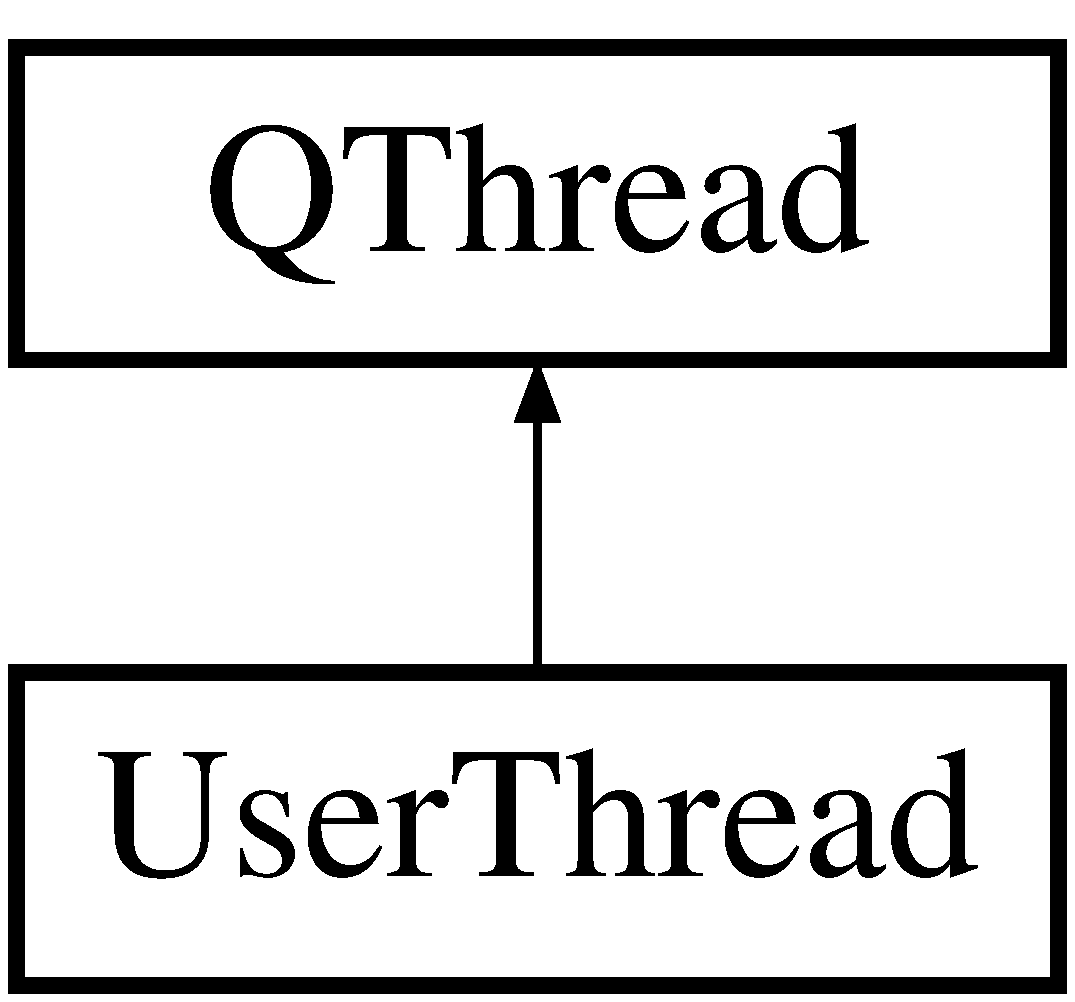
\includegraphics[height=2.000000cm]{class_d_o_1_1_user_thread}
\end{center}
\end{figure}
\subsection*{Public Slots}
\begin{DoxyCompactItemize}
\item 
\hypertarget{group___graphics_internal_ga17e8cfdefacfb6fc452b7505a5ddad42}{void {\bfseries listen\-To\-Window\-Events} ()}\label{group___graphics_internal_ga17e8cfdefacfb6fc452b7505a5ddad42}

\item 
\hypertarget{group___graphics_internal_ga211d59c0a6baf6072e762c542472efe6}{void {\bfseries pressed\-Mouse\-Buttons} (int x, int \hyperlink{group___channel_accessors_gac90c52c5b3a7b2a7e3761e6e84f25778}{y}, Qt\-::\-Mouse\-Buttons buttons)}\label{group___graphics_internal_ga211d59c0a6baf6072e762c542472efe6}

\item 
\hypertarget{group___graphics_internal_gaf3120a375a321654553779cf030a9508}{void {\bfseries pressed\-Key} (int key)}\label{group___graphics_internal_gaf3120a375a321654553779cf030a9508}

\item 
\hypertarget{group___graphics_internal_gab4b152469c806312bcb7fbbbcbccb6dc}{void {\bfseries closed\-Window} ()}\label{group___graphics_internal_gab4b152469c806312bcb7fbbbcbccb6dc}

\item 
\hypertarget{group___graphics_internal_ga2ea8e392e6f4fcb9fdb5b76e7bb02953}{void {\bfseries received\-Event} (\hyperlink{struct_d_o_1_1_event}{Event} e)}\label{group___graphics_internal_ga2ea8e392e6f4fcb9fdb5b76e7bb02953}

\end{DoxyCompactItemize}
\subsection*{Public Member Functions}
\begin{DoxyCompactItemize}
\item 
\hypertarget{group___graphics_internal_ga520a11a377381bb516be45e6d5564a51}{{\bfseries User\-Thread} (Q\-Object $\ast$parent=0)}\label{group___graphics_internal_ga520a11a377381bb516be45e6d5564a51}

\item 
\hypertarget{group___graphics_internal_ga205cb5d1ecd1b0a8473ec0233724b8d9}{void {\bfseries register\-User\-Main} (int($\ast$user\-Main)(void))}\label{group___graphics_internal_ga205cb5d1ecd1b0a8473ec0233724b8d9}

\item 
\hypertarget{group___graphics_internal_gaacb94ff196c97609974b21595461e093}{void {\bfseries milli\-Sleep} (int msec)}\label{group___graphics_internal_gaacb94ff196c97609974b21595461e093}

\item 
\hypertarget{group___graphics_internal_ga64b410b838a1bda3e1a16f1b4171eb99}{void {\bfseries micro\-Sleep} (int usec)}\label{group___graphics_internal_ga64b410b838a1bda3e1a16f1b4171eb99}

\item 
\hypertarget{group___graphics_internal_ga4ac6dfc380bd4b753f2433a081a51942}{int {\bfseries get\-Mouse} (int \&x, int \&\hyperlink{group___channel_accessors_gac90c52c5b3a7b2a7e3761e6e84f25778}{y})}\label{group___graphics_internal_ga4ac6dfc380bd4b753f2433a081a51942}

\item 
\hypertarget{group___graphics_internal_gaa5cbe387ac3ae002933daa7d8371d17b}{int {\bfseries get\-Key} ()}\label{group___graphics_internal_gaa5cbe387ac3ae002933daa7d8371d17b}

\item 
\hypertarget{group___graphics_internal_ga66b52a9903f2651cd0968a9282d9d740}{void {\bfseries get\-Event} (\hyperlink{struct_d_o_1_1_event}{Event} \&e)}\label{group___graphics_internal_ga66b52a9903f2651cd0968a9282d9d740}

\end{DoxyCompactItemize}
\subsection*{Protected Member Functions}
\begin{DoxyCompactItemize}
\item 
\hypertarget{group___graphics_internal_ga13a43e6d814de94978c515cb084873b1}{void {\bfseries run} ()}\label{group___graphics_internal_ga13a43e6d814de94978c515cb084873b1}

\end{DoxyCompactItemize}


\subsection{Detailed Description}
This is actually where we actually call the drawing commands. 

The documentation for this class was generated from the following file\-:\begin{DoxyCompactItemize}
\item 
src/\-D\-O/\-Graphics/\-Derived\-Q\-Objects/\hyperlink{_user_thread_8hpp}{User\-Thread.\-hpp}\end{DoxyCompactItemize}

\hypertarget{struct_d_o_1_1_v}{\section{V Struct Reference}
\label{struct_d_o_1_1_v}\index{V@{V}}
}


Second chrominance name (Y\-U\-V) or Value channel name (H\-S\-V).  




{\ttfamily \#include $<$Color.\-hpp$>$}



\subsection{Detailed Description}
Second chrominance name (Y\-U\-V) or Value channel name (H\-S\-V). 

The documentation for this struct was generated from the following file\-:\begin{DoxyCompactItemize}
\item 
src/\-D\-O/\-Core/\hyperlink{_color_8hpp}{Color.\-hpp}\end{DoxyCompactItemize}

\hypertarget{struct_d_o_1_1_meta_1_1_vector3}{\section{Vector3$<$ T0\-\_\-, T1\-\_\-, T2\-\_\- $>$ Struct Template Reference}
\label{struct_d_o_1_1_meta_1_1_vector3}\index{Vector3$<$ T0\-\_\-, T1\-\_\-, T2\-\_\- $>$@{Vector3$<$ T0\-\_\-, T1\-\_\-, T2\-\_\- $>$}}
}


3\-D vector of types.  




{\ttfamily \#include $<$Meta.\-hpp$>$}

\subsection*{Public Types}
\begin{DoxyCompactItemize}
\item 
enum \{ {\bfseries size} = 3
 \}
\item 
\hypertarget{struct_d_o_1_1_meta_1_1_vector3_a6f4dd1548d86d57a7e5bdf98e74025cd}{typedef T0\-\_\- \hyperlink{struct_d_o_1_1_meta_1_1_vector3_a6f4dd1548d86d57a7e5bdf98e74025cd}{T0}}\label{struct_d_o_1_1_meta_1_1_vector3_a6f4dd1548d86d57a7e5bdf98e74025cd}

\begin{DoxyCompactList}\small\item\em Element 0 is type T0. \end{DoxyCompactList}\item 
\hypertarget{struct_d_o_1_1_meta_1_1_vector3_ae11d8678c6e0ac8e98f27b6dfdb5d73e}{typedef T1\-\_\- \hyperlink{struct_d_o_1_1_meta_1_1_vector3_ae11d8678c6e0ac8e98f27b6dfdb5d73e}{T1}}\label{struct_d_o_1_1_meta_1_1_vector3_ae11d8678c6e0ac8e98f27b6dfdb5d73e}

\begin{DoxyCompactList}\small\item\em Element 1 is type T1. \end{DoxyCompactList}\item 
\hypertarget{struct_d_o_1_1_meta_1_1_vector3_acbff7929c9f657ca83ddd209a08f7d62}{typedef T2\-\_\- \hyperlink{struct_d_o_1_1_meta_1_1_vector3_acbff7929c9f657ca83ddd209a08f7d62}{T2}}\label{struct_d_o_1_1_meta_1_1_vector3_acbff7929c9f657ca83ddd209a08f7d62}

\begin{DoxyCompactList}\small\item\em Element 2 is type T2. \end{DoxyCompactList}\end{DoxyCompactItemize}


\subsection{Detailed Description}
\subsubsection*{template$<$typename T0\-\_\-, typename T1\-\_\-, typename T2\-\_\-$>$struct D\-O\-::\-Meta\-::\-Vector3$<$ T0\-\_\-, T1\-\_\-, T2\-\_\- $>$}

3\-D vector of types. 

The documentation for this struct was generated from the following file\-:\begin{DoxyCompactItemize}
\item 
src/\-D\-O/\-Core/\hyperlink{_meta_8hpp}{Meta.\-hpp}\end{DoxyCompactItemize}

\hypertarget{struct_d_o_1_1_meta_1_1_vector4}{\section{Vector4$<$ T0\-\_\-, T1\-\_\-, T2\-\_\-, T3\-\_\- $>$ Struct Template Reference}
\label{struct_d_o_1_1_meta_1_1_vector4}\index{Vector4$<$ T0\-\_\-, T1\-\_\-, T2\-\_\-, T3\-\_\- $>$@{Vector4$<$ T0\-\_\-, T1\-\_\-, T2\-\_\-, T3\-\_\- $>$}}
}


4\-D vector of types.  




{\ttfamily \#include $<$Meta.\-hpp$>$}

\subsection*{Public Types}
\begin{DoxyCompactItemize}
\item 
enum \{ {\bfseries size} = 4
 \}
\item 
\hypertarget{struct_d_o_1_1_meta_1_1_vector4_a6f4dd1548d86d57a7e5bdf98e74025cd}{typedef T0\-\_\- \hyperlink{struct_d_o_1_1_meta_1_1_vector4_a6f4dd1548d86d57a7e5bdf98e74025cd}{T0}}\label{struct_d_o_1_1_meta_1_1_vector4_a6f4dd1548d86d57a7e5bdf98e74025cd}

\begin{DoxyCompactList}\small\item\em Element 0 is type T0. \end{DoxyCompactList}\item 
\hypertarget{struct_d_o_1_1_meta_1_1_vector4_ae11d8678c6e0ac8e98f27b6dfdb5d73e}{typedef T1\-\_\- \hyperlink{struct_d_o_1_1_meta_1_1_vector4_ae11d8678c6e0ac8e98f27b6dfdb5d73e}{T1}}\label{struct_d_o_1_1_meta_1_1_vector4_ae11d8678c6e0ac8e98f27b6dfdb5d73e}

\begin{DoxyCompactList}\small\item\em Element 1 is type T1. \end{DoxyCompactList}\item 
\hypertarget{struct_d_o_1_1_meta_1_1_vector4_acbff7929c9f657ca83ddd209a08f7d62}{typedef T2\-\_\- \hyperlink{struct_d_o_1_1_meta_1_1_vector4_acbff7929c9f657ca83ddd209a08f7d62}{T2}}\label{struct_d_o_1_1_meta_1_1_vector4_acbff7929c9f657ca83ddd209a08f7d62}

\begin{DoxyCompactList}\small\item\em Element 2 is type T2. \end{DoxyCompactList}\item 
\hypertarget{struct_d_o_1_1_meta_1_1_vector4_af4c555323f12d8f0d74cbece2c5c4a47}{typedef T3\-\_\- \hyperlink{struct_d_o_1_1_meta_1_1_vector4_af4c555323f12d8f0d74cbece2c5c4a47}{T3}}\label{struct_d_o_1_1_meta_1_1_vector4_af4c555323f12d8f0d74cbece2c5c4a47}

\begin{DoxyCompactList}\small\item\em Element 3 is type T3. \end{DoxyCompactList}\end{DoxyCompactItemize}


\subsection{Detailed Description}
\subsubsection*{template$<$typename T0\-\_\-, typename T1\-\_\-, typename T2\-\_\-, typename T3\-\_\-$>$struct D\-O\-::\-Meta\-::\-Vector4$<$ T0\-\_\-, T1\-\_\-, T2\-\_\-, T3\-\_\- $>$}

4\-D vector of types. 

The documentation for this struct was generated from the following file\-:\begin{DoxyCompactItemize}
\item 
src/\-D\-O/\-Core/\hyperlink{_meta_8hpp}{Meta.\-hpp}\end{DoxyCompactItemize}

\hypertarget{struct_d_o_1_1_y}{\section{Y Struct Reference}
\label{struct_d_o_1_1_y}\index{Y@{Y}}
}


Yellow channel name (C\-M\-Y\-K) or Luminance channel name (Y\-U\-V).  




{\ttfamily \#include $<$Color.\-hpp$>$}



\subsection{Detailed Description}
Yellow channel name (C\-M\-Y\-K) or Luminance channel name (Y\-U\-V). 

The documentation for this struct was generated from the following file\-:\begin{DoxyCompactItemize}
\item 
src/\-D\-O/\-Core/\hyperlink{_color_8hpp}{Color.\-hpp}\end{DoxyCompactItemize}

\chapter{File Documentation}
\hypertarget{_core_8hpp}{\section{src/\-D\-O/\-Core.hpp File Reference}
\label{_core_8hpp}\index{src/\-D\-O/\-Core.\-hpp@{src/\-D\-O/\-Core.\-hpp}}
}


Master header file of the Core module.  


{\ttfamily \#include $<$Eigen/\-Eigen$>$}\\*
{\ttfamily \#include $<$algorithm$>$}\\*
{\ttfamily \#include $<$ctime$>$}\\*
{\ttfamily \#include $<$exception$>$}\\*
{\ttfamily \#include $<$fstream$>$}\\*
{\ttfamily \#include $<$iostream$>$}\\*
{\ttfamily \#include $<$iterator$>$}\\*
{\ttfamily \#include $<$limits$>$}\\*
{\ttfamily \#include $<$map$>$}\\*
{\ttfamily \#include $<$numeric$>$}\\*
{\ttfamily \#include $<$queue$>$}\\*
{\ttfamily \#include $<$stack$>$}\\*
{\ttfamily \#include $<$string$>$}\\*
{\ttfamily \#include $<$sstream$>$}\\*
{\ttfamily \#include $<$stdexcept$>$}\\*
{\ttfamily \#include \char`\"{}Core/\-Eigen\-Extension.\-hpp\char`\"{}}\\*
{\ttfamily \#include \char`\"{}Core/\-Meta.\-hpp\char`\"{}}\\*
{\ttfamily \#include \char`\"{}Core/\-Static\-Assert.\-hpp\char`\"{}}\\*
{\ttfamily \#include \char`\"{}Core/\-Stringify.\-hpp\char`\"{}}\\*
{\ttfamily \#include \char`\"{}Core/\-Timer.\-hpp\char`\"{}}\\*
{\ttfamily \#include \char`\"{}Core/\-Color.\-hpp\char`\"{}}\\*
{\ttfamily \#include \char`\"{}Core/\-Locator.\-hpp\char`\"{}}\\*
{\ttfamily \#include \char`\"{}Core/\-Multi\-Array.\-hpp\char`\"{}}\\*
{\ttfamily \#include \char`\"{}Core/\-Sparse\-Multi\-Array.\-hpp\char`\"{}}\\*
{\ttfamily \#include \char`\"{}Core/\-Image.\-hpp\char`\"{}}\\*
{\ttfamily \#include \char`\"{}Core/\-Tree.\-hpp\char`\"{}}\\*
\subsection*{Namespaces}
\begin{DoxyCompactItemize}
\item 
namespace \hyperlink{namespace_d_o}{D\-O}
\begin{DoxyCompactList}\small\item\em The library namespace. \end{DoxyCompactList}\end{DoxyCompactItemize}
\subsection*{Macros}
\begin{DoxyCompactItemize}
\item 
\hypertarget{_core_8hpp_a525335710b53cb064ca56b936120431e}{\#define \hyperlink{_core_8hpp_a525335710b53cb064ca56b936120431e}{\-\_\-\-U\-S\-E\-\_\-\-M\-A\-T\-H\-\_\-\-D\-E\-F\-I\-N\-E\-S}}\label{_core_8hpp_a525335710b53cb064ca56b936120431e}

\begin{DoxyCompactList}\small\item\em Activate by default math constants. \end{DoxyCompactList}\item 
\hypertarget{group___core_ga6befbca3f4c07866e5a0b6b255b6a469}{\#define \hyperlink{group___core_ga6befbca3f4c07866e5a0b6b255b6a469}{B\-E\-G\-I\-N\-\_\-\-N\-A\-M\-E\-S\-P\-A\-C\-E\-\_\-\-D\-O}~namespace D\-O \{}\label{group___core_ga6befbca3f4c07866e5a0b6b255b6a469}

\begin{DoxyCompactList}\small\item\em Opening macro whose sole purpose is to increase the namespace visibility. \end{DoxyCompactList}\item 
\hypertarget{group___core_gace84578be62b4659157bfae5b1e7b9f4}{\#define \hyperlink{group___core_gace84578be62b4659157bfae5b1e7b9f4}{E\-N\-D\-\_\-\-N\-A\-M\-E\-S\-P\-A\-C\-E\-\_\-\-D\-O}~\} /$\ast$ namespace D\-O $\ast$/}\label{group___core_gace84578be62b4659157bfae5b1e7b9f4}

\begin{DoxyCompactList}\small\item\em Closing macro whose sole purpose is to increase the namespace visibility. \end{DoxyCompactList}\item 
\#define \hyperlink{group___core_ga3a1adaa43f4f9abbba0e666652a3756c}{src\-Path}(s)~(s)
\begin{DoxyCompactList}\small\item\em Returns the full path of a file when C\-Make is used. \end{DoxyCompactList}\item 
\#define \hyperlink{group___core_ga6dcd6c29c77233d5b21cda46b3aad899}{string\-Src\-Path}(s)~(s)
\begin{DoxyCompactList}\small\item\em Returns the full path of a file when C\-Make is used. \end{DoxyCompactList}\end{DoxyCompactItemize}


\subsection{Detailed Description}
Master header file of the Core module. 
\hypertarget{_color_8hpp}{\section{src/\-D\-O/\-Core/\-Color.hpp File Reference}
\label{_color_8hpp}\index{src/\-D\-O/\-Core/\-Color.\-hpp@{src/\-D\-O/\-Core/\-Color.\-hpp}}
}
\subsection*{Classes}
\begin{DoxyCompactItemize}
\item 
struct \hyperlink{struct_d_o_1_1_r}{R}
\begin{DoxyCompactList}\small\item\em Red channel name (R\-G\-B, R\-G\-B\-A). \end{DoxyCompactList}\item 
struct \hyperlink{struct_d_o_1_1_g}{G}
\begin{DoxyCompactList}\small\item\em Green channel name (R\-G\-B, R\-G\-B\-A). \end{DoxyCompactList}\item 
struct \hyperlink{struct_d_o_1_1_b}{B}
\begin{DoxyCompactList}\small\item\em Blue channel name (R\-G\-B, R\-G\-B\-A). \end{DoxyCompactList}\item 
struct \hyperlink{struct_d_o_1_1_a}{A}
\begin{DoxyCompactList}\small\item\em Alpha channel name (R\-G\-B, R\-G\-B\-A). \end{DoxyCompactList}\item 
struct \hyperlink{struct_d_o_1_1_c}{C}
\begin{DoxyCompactList}\small\item\em Cyan channel name (C\-M\-Y\-K). \end{DoxyCompactList}\item 
struct \hyperlink{struct_d_o_1_1_m}{M}
\begin{DoxyCompactList}\small\item\em Magenta channel name (C\-M\-Y\-K). \end{DoxyCompactList}\item 
struct \hyperlink{struct_d_o_1_1_y}{Y}
\begin{DoxyCompactList}\small\item\em Yellow channel name (C\-M\-Y\-K) or Luminance channel name (Y\-U\-V). \end{DoxyCompactList}\item 
struct \hyperlink{struct_d_o_1_1_k}{K}
\begin{DoxyCompactList}\small\item\em Black channel name (C\-M\-Y\-K). \end{DoxyCompactList}\item 
struct \hyperlink{struct_d_o_1_1_u}{U}
\begin{DoxyCompactList}\small\item\em First chrominance name (Y\-U\-V). \end{DoxyCompactList}\item 
struct \hyperlink{struct_d_o_1_1_v}{V}
\begin{DoxyCompactList}\small\item\em Second chrominance name (Y\-U\-V) or Value channel name (H\-S\-V). \end{DoxyCompactList}\item 
struct \hyperlink{struct_d_o_1_1_h}{H}
\begin{DoxyCompactList}\small\item\em Hue channel name (H\-S\-V). \end{DoxyCompactList}\item 
struct \hyperlink{struct_d_o_1_1_s}{S}
\begin{DoxyCompactList}\small\item\em Saturation channel name (H\-S\-V). \end{DoxyCompactList}\item 
struct \hyperlink{struct_d_o_1_1_gray}{Gray}
\begin{DoxyCompactList}\small\item\em Grayscale color space. \end{DoxyCompactList}\item 
class \hyperlink{class_d_o_1_1_color}{Color$<$ T, Layout $>$}
\begin{DoxyCompactList}\small\item\em Lightweight template color class with some flexibility. \end{DoxyCompactList}\item 
struct \hyperlink{struct_d_o_1_1_channel_traits}{Channel\-Traits$<$ T $>$}
\begin{DoxyCompactList}\small\item\em Channel traits class. \end{DoxyCompactList}\item 
struct \hyperlink{struct_d_o_1_1_color_traits}{Color\-Traits$<$ Color\-\_\- $>$}
\begin{DoxyCompactList}\small\item\em \hyperlink{class_d_o_1_1_color}{Color} traits class. \end{DoxyCompactList}\item 
struct \hyperlink{struct_d_o_1_1_color_traits_3_01_matrix_3_01_channel_type___00_013_00_011_01_4_01_4}{Color\-Traits$<$ Matrix$<$ Channel\-Type\-\_\-, 3, 1 $>$ $>$}
\begin{DoxyCompactList}\small\item\em Specialized color traits class for 3\-D color types. \end{DoxyCompactList}\item 
struct \hyperlink{struct_d_o_1_1_color_traits_3_01_matrix_3_01_channel_type___00_014_00_011_01_4_01_4}{Color\-Traits$<$ Matrix$<$ Channel\-Type\-\_\-, 4, 1 $>$ $>$}
\begin{DoxyCompactList}\small\item\em Specialized color traits class for 4\-D color types. \end{DoxyCompactList}\item 
struct \hyperlink{struct_d_o_1_1_color_traits_3_01uchar_01_4}{Color\-Traits$<$ uchar $>$}
\begin{DoxyCompactList}\small\item\em Specialized color traits class for 'uchar' grayscale color. \end{DoxyCompactList}\item 
struct \hyperlink{struct_d_o_1_1_color_traits_3_01ushort_01_4}{Color\-Traits$<$ ushort $>$}
\begin{DoxyCompactList}\small\item\em Specialized color traits class for 'ushort' grayscale color. \end{DoxyCompactList}\item 
struct \hyperlink{struct_d_o_1_1_color_traits_3_01uint_01_4}{Color\-Traits$<$ uint $>$}
\begin{DoxyCompactList}\small\item\em Specialized color traits class for 'uint' grayscale color. \end{DoxyCompactList}\item 
struct \hyperlink{struct_d_o_1_1_color_traits_3_01char_01_4}{Color\-Traits$<$ char $>$}
\begin{DoxyCompactList}\small\item\em Specialized color traits class for 'char' grayscale color. \end{DoxyCompactList}\item 
struct \hyperlink{struct_d_o_1_1_color_traits_3_01short_01_4}{Color\-Traits$<$ short $>$}
\begin{DoxyCompactList}\small\item\em Specialized color traits class for 'short' grayscale color. \end{DoxyCompactList}\item 
struct \hyperlink{struct_d_o_1_1_color_traits_3_01int_01_4}{Color\-Traits$<$ int $>$}
\begin{DoxyCompactList}\small\item\em Specialized color traits class for 'int' grayscale color. \end{DoxyCompactList}\item 
struct \hyperlink{struct_d_o_1_1_color_traits_3_01float_01_4}{Color\-Traits$<$ float $>$}
\begin{DoxyCompactList}\small\item\em Specialized color traits class for 'float' grayscale color. \end{DoxyCompactList}\item 
struct \hyperlink{struct_d_o_1_1_color_traits_3_01double_01_4}{Color\-Traits$<$ double $>$}
\begin{DoxyCompactList}\small\item\em Specialized color traits class for 'double' grayscale color. \end{DoxyCompactList}\end{DoxyCompactItemize}
\subsection*{Namespaces}
\begin{DoxyCompactItemize}
\item 
namespace \hyperlink{namespace_d_o}{D\-O}
\begin{DoxyCompactList}\small\item\em The library namespace. \end{DoxyCompactList}\end{DoxyCompactItemize}
\subsection*{Macros}
\begin{DoxyCompactItemize}
\item 
\#define \hyperlink{group___channel_accessors_ga17a132ee4905c132201008787b93e336}{D\-E\-F\-I\-N\-E\-\_\-\-C\-O\-L\-O\-R\-\_\-\-C\-H\-A\-N\-N\-E\-L\-\_\-\-G\-E\-T\-T\-E\-R\-S}(channel\-Name, channel\-Tag)
\begin{DoxyCompactList}\small\item\em Macro that defines short mutable and non-\/mutable channel accessors. \end{DoxyCompactList}\item 
\hypertarget{group___color_traits_ga02ba6c4706c9e998a2fa50912709bac2}{\#define \hyperlink{group___color_traits_ga02ba6c4706c9e998a2fa50912709bac2}{D\-E\-F\-I\-N\-E\-\_\-\-G\-R\-A\-Y\-\_\-\-C\-O\-L\-O\-R\-\_\-\-T\-R\-A\-I\-T\-S}(gray\-\_\-channel\-\_\-t)}\label{group___color_traits_ga02ba6c4706c9e998a2fa50912709bac2}

\begin{DoxyCompactList}\small\item\em Macro that defines specialized color traits classes for grayscale types. \end{DoxyCompactList}\item 
\#define \hyperlink{group___color_conversion_gac0e4b5dd70b28feca22cc770d9862a8b}{C\-O\-L\-O\-R\-\_\-\-C\-O\-N\-V\-E\-R\-S\-I\-O\-N\-\_\-\-B\-E\-T\-W\-E\-E\-N\-\_\-\-G\-R\-A\-Y\-\_\-\-A\-N\-D\-\_\-\-R\-G\-B}(Gray\-Type)
\begin{DoxyCompactList}\small\item\em Color conversion between gray and R\-G\-B color spaces. \end{DoxyCompactList}\item 
\#define \hyperlink{group___color_conversion_gadcb0f8382525554854f5cb0ffa5ffeee}{D\-E\-F\-I\-N\-E\-\_\-\-C\-O\-L\-O\-R\-\_\-\-C\-O\-N\-V\-E\-R\-S\-I\-O\-N\-\_\-\-B\-E\-T\-W\-E\-E\-N\-\_\-\-I\-N\-T\-E\-G\-R\-A\-L\-\_\-\-G\-R\-A\-Y\-\_\-\-T\-Y\-P\-E\-S}(Gray1, Gray2)
\begin{DoxyCompactList}\small\item\em Color conversion between integral gray colors. \end{DoxyCompactList}\item 
\#define \hyperlink{group___color_conversion_gad00b96d2364bfb1473d0a12dbd5b26c5}{D\-E\-F\-I\-N\-E\-\_\-\-C\-O\-L\-O\-R\-\_\-\-C\-O\-N\-V\-E\-R\-S\-I\-O\-N\-\_\-\-B\-E\-T\-W\-E\-E\-N\-\_\-\-I\-N\-T\-\_\-\-A\-N\-D\-\_\-\-F\-L\-O\-A\-T\-I\-N\-G\-\_\-\-T\-Y\-P\-E\-S}(Float, Int)
\begin{DoxyCompactList}\small\item\em Color conversion between integral and floating point gray colors. \end{DoxyCompactList}\item 
\#define \hyperlink{group___color_types_ga83f7f072aef53405d76e922f4a2a84a5}{D\-E\-F\-I\-N\-E\-\_\-\-G\-E\-N\-E\-R\-I\-C\-\_\-\-C\-O\-L\-O\-R\-\_\-\-T\-Y\-P\-E\-D\-E\-F\-S}(N)
\begin{DoxyCompactList}\small\item\em Macro for generic color typedefs. \end{DoxyCompactList}\item 
\#define \hyperlink{group___color_types_ga51fca00f14d0e12f57b41d7387fc678c}{D\-E\-F\-I\-N\-E\-\_\-\-C\-O\-L\-O\-R\-\_\-\-T\-Y\-P\-E\-S}(colorspace)
\begin{DoxyCompactList}\small\item\em Macro for color typedefs. \end{DoxyCompactList}\item 
\#define \hyperlink{group___primary_colors_ga372b1b173b9a8fcb12af311790630867}{D\-E\-F\-I\-N\-E\-\_\-\-C\-O\-L\-O\-R\-\_\-\-C\-O\-N\-S\-T\-A\-N\-T}(Name, function)
\begin{DoxyCompactList}\small\item\em Primary color definition. \end{DoxyCompactList}\end{DoxyCompactItemize}
\subsection*{Typedefs}
\begin{DoxyCompactItemize}
\item 
\hypertarget{group___color_space_ga52ed562e9155b12e5395633a01476810}{typedef Meta\-::\-Vector4$<$ R, G, B, A $>$ \hyperlink{group___color_space_ga52ed562e9155b12e5395633a01476810}{Rgba}}\label{group___color_space_ga52ed562e9155b12e5395633a01476810}

\begin{DoxyCompactList}\small\item\em R\-G\-B\-A color space and layout. \end{DoxyCompactList}\item 
\hypertarget{group___color_space_gac3a42db968dfe7d65b7b74f49de821c3}{typedef Meta\-::\-Vector4$<$ A, R, G, B $>$ \hyperlink{group___color_space_gac3a42db968dfe7d65b7b74f49de821c3}{Argb}}\label{group___color_space_gac3a42db968dfe7d65b7b74f49de821c3}

\begin{DoxyCompactList}\small\item\em A\-R\-G\-B color space and layout. \end{DoxyCompactList}\item 
\hypertarget{group___color_space_gae0496dd76c54f129381947440d56a874}{typedef Meta\-::\-Vector4$<$ A, B, G, R $>$ \hyperlink{group___color_space_gae0496dd76c54f129381947440d56a874}{Abgr}}\label{group___color_space_gae0496dd76c54f129381947440d56a874}

\begin{DoxyCompactList}\small\item\em A\-B\-G\-R color space and layout. \end{DoxyCompactList}\item 
\hypertarget{group___color_space_gadb2e9d99bf441a224f4d628ad62a0bd2}{typedef Meta\-::\-Vector4$<$ B, R, G, A $>$ \hyperlink{group___color_space_gadb2e9d99bf441a224f4d628ad62a0bd2}{Bgra}}\label{group___color_space_gadb2e9d99bf441a224f4d628ad62a0bd2}

\begin{DoxyCompactList}\small\item\em B\-G\-R\-A color space and layout. \end{DoxyCompactList}\item 
\hypertarget{group___color_space_ga3d376efd2059bb15b8fd696946e051ff}{typedef Meta\-::\-Vector4$<$ C, M, Y, K $>$ \hyperlink{group___color_space_ga3d376efd2059bb15b8fd696946e051ff}{Cmyk}}\label{group___color_space_ga3d376efd2059bb15b8fd696946e051ff}

\begin{DoxyCompactList}\small\item\em C\-M\-Y\-K color space and layout. \end{DoxyCompactList}\item 
\hypertarget{group___color_space_gaad92fea51e98e11252ac86f2c8665d13}{typedef Meta\-::\-Vector3$<$ R, G, B $>$ \hyperlink{group___color_space_gaad92fea51e98e11252ac86f2c8665d13}{Rgb}}\label{group___color_space_gaad92fea51e98e11252ac86f2c8665d13}

\begin{DoxyCompactList}\small\item\em R\-G\-B color space and layout. \end{DoxyCompactList}\item 
\hypertarget{group___color_space_ga9a1cd8af7d2fb33189763c2edb5f262b}{typedef Meta\-::\-Vector3$<$ B, G, R $>$ \hyperlink{group___color_space_ga9a1cd8af7d2fb33189763c2edb5f262b}{Bgr}}\label{group___color_space_ga9a1cd8af7d2fb33189763c2edb5f262b}

\begin{DoxyCompactList}\small\item\em B\-G\-R color space and layout. \end{DoxyCompactList}\item 
\hypertarget{group___color_space_ga8d04b5aa0ecd455aa29da0987b106ad0}{typedef Meta\-::\-Vector3$<$ Y, U, V $>$ \hyperlink{group___color_space_ga8d04b5aa0ecd455aa29da0987b106ad0}{Yuv}}\label{group___color_space_ga8d04b5aa0ecd455aa29da0987b106ad0}

\begin{DoxyCompactList}\small\item\em Y\-U\-V color space and layout. \end{DoxyCompactList}\item 
\hypertarget{group___color_space_gaef854af3bd9309a9d2cfec268e7ccb9b}{typedef Meta\-::\-Vector3$<$ H, S, V $>$ \hyperlink{group___color_space_gaef854af3bd9309a9d2cfec268e7ccb9b}{Hsv}}\label{group___color_space_gaef854af3bd9309a9d2cfec268e7ccb9b}

\begin{DoxyCompactList}\small\item\em H\-S\-V color space and layout. \end{DoxyCompactList}\item 
\hypertarget{group___color_types_ga71a5d51cd25b220d9cb09cc4ec231b57}{typedef uchar \hyperlink{group___color_types_ga71a5d51cd25b220d9cb09cc4ec231b57}{gray8}}\label{group___color_types_ga71a5d51cd25b220d9cb09cc4ec231b57}

\begin{DoxyCompactList}\small\item\em self-\/explanatory. \end{DoxyCompactList}\item 
\hypertarget{group___color_types_ga08ae2e1a2fcf5d04bce4407dad5c6744}{typedef char \hyperlink{group___color_types_ga08ae2e1a2fcf5d04bce4407dad5c6744}{gray8s}}\label{group___color_types_ga08ae2e1a2fcf5d04bce4407dad5c6744}

\begin{DoxyCompactList}\small\item\em self-\/explanatory. \end{DoxyCompactList}\item 
\hypertarget{group___color_types_ga97476c670307c0b9fb13502e618fa3f2}{typedef ushort \hyperlink{group___color_types_ga97476c670307c0b9fb13502e618fa3f2}{gray16}}\label{group___color_types_ga97476c670307c0b9fb13502e618fa3f2}

\begin{DoxyCompactList}\small\item\em self-\/explanatory. \end{DoxyCompactList}\item 
\hypertarget{group___color_types_ga7b4d8c29b4d1573e4c6d00de9c18154c}{typedef short \hyperlink{group___color_types_ga7b4d8c29b4d1573e4c6d00de9c18154c}{gray16s}}\label{group___color_types_ga7b4d8c29b4d1573e4c6d00de9c18154c}

\begin{DoxyCompactList}\small\item\em self-\/explanatory. \end{DoxyCompactList}\item 
\hypertarget{group___color_types_gaaea3b22bdc6fbbc1f8d7d53f0ba8f098}{typedef uint \hyperlink{group___color_types_gaaea3b22bdc6fbbc1f8d7d53f0ba8f098}{gray32}}\label{group___color_types_gaaea3b22bdc6fbbc1f8d7d53f0ba8f098}

\begin{DoxyCompactList}\small\item\em self-\/explanatory. \end{DoxyCompactList}\item 
\hypertarget{group___color_types_gac9a11db63526348331dcb825f6830989}{typedef int \hyperlink{group___color_types_gac9a11db63526348331dcb825f6830989}{gray32s}}\label{group___color_types_gac9a11db63526348331dcb825f6830989}

\begin{DoxyCompactList}\small\item\em self-\/explanatory. \end{DoxyCompactList}\item 
\hypertarget{group___color_types_ga9c8a72eb9c04233172157ab5e7d0be22}{typedef float \hyperlink{group___color_types_ga9c8a72eb9c04233172157ab5e7d0be22}{gray32f}}\label{group___color_types_ga9c8a72eb9c04233172157ab5e7d0be22}

\begin{DoxyCompactList}\small\item\em self-\/explanatory. \end{DoxyCompactList}\item 
\hypertarget{group___color_types_gaf5100147ede5b7f434dc4238668a3c13}{typedef double \hyperlink{group___color_types_gaf5100147ede5b7f434dc4238668a3c13}{gray64f}}\label{group___color_types_gaf5100147ede5b7f434dc4238668a3c13}

\begin{DoxyCompactList}\small\item\em self-\/explanatory. \end{DoxyCompactList}\item 
\hypertarget{group___color_types_ga018b76cd00a4f9dca7dd06246d5bd3aa}{typedef Matrix$<$ uchar, 3, 1 $>$ \hyperlink{group___color_types_ga018b76cd00a4f9dca7dd06246d5bd3aa}{Color3ub}}\label{group___color_types_ga018b76cd00a4f9dca7dd06246d5bd3aa}

\begin{DoxyCompactList}\small\item\em \hyperlink{class_d_o_1_1_color}{Color}\{Num\-Channels\}\{Channel\-Type\}. \end{DoxyCompactList}\item 
\hypertarget{group___color_types_ga1f41bb6772fe8bff45c855c578c739d1}{typedef Matrix$<$ char, 3, 1 $>$ \hyperlink{group___color_types_ga1f41bb6772fe8bff45c855c578c739d1}{Color3b}}\label{group___color_types_ga1f41bb6772fe8bff45c855c578c739d1}

\begin{DoxyCompactList}\small\item\em \hyperlink{class_d_o_1_1_color}{Color}\{Num\-Channels\}\{Channel\-Type\}. \end{DoxyCompactList}\item 
\hypertarget{group___color_types_ga4db675bfc61fec77a5524f279f46d07a}{typedef Matrix$<$ ushort, 3, 1 $>$ \hyperlink{group___color_types_ga4db675bfc61fec77a5524f279f46d07a}{Color3us}}\label{group___color_types_ga4db675bfc61fec77a5524f279f46d07a}

\begin{DoxyCompactList}\small\item\em \hyperlink{class_d_o_1_1_color}{Color}\{Num\-Channels\}\{Channel\-Type\}. \end{DoxyCompactList}\item 
\hypertarget{group___color_types_gabd8ed6efb783441fd8fb924a32c6848b}{typedef Matrix$<$ short, 3, 1 $>$ \hyperlink{group___color_types_gabd8ed6efb783441fd8fb924a32c6848b}{Color3s}}\label{group___color_types_gabd8ed6efb783441fd8fb924a32c6848b}

\begin{DoxyCompactList}\small\item\em \hyperlink{class_d_o_1_1_color}{Color}\{Num\-Channels\}\{Channel\-Type\}. \end{DoxyCompactList}\item 
\hypertarget{group___color_types_ga7b8b491888795ce0cd0a75d017db1a74}{typedef Matrix$<$ uint, 3, 1 $>$ \hyperlink{group___color_types_ga7b8b491888795ce0cd0a75d017db1a74}{Color3ui}}\label{group___color_types_ga7b8b491888795ce0cd0a75d017db1a74}

\begin{DoxyCompactList}\small\item\em \hyperlink{class_d_o_1_1_color}{Color}\{Num\-Channels\}\{Channel\-Type\}. \end{DoxyCompactList}\item 
\hypertarget{group___color_types_gabe1176859fd849a93edd59c687680805}{typedef Matrix$<$ int, 3, 1 $>$ \hyperlink{group___color_types_gabe1176859fd849a93edd59c687680805}{Color3i}}\label{group___color_types_gabe1176859fd849a93edd59c687680805}

\begin{DoxyCompactList}\small\item\em \hyperlink{class_d_o_1_1_color}{Color}\{Num\-Channels\}\{Channel\-Type\}. \end{DoxyCompactList}\item 
\hypertarget{group___color_types_ga4df0906a5f67901886b7d42343632ccb}{typedef Matrix$<$ float, 3, 1 $>$ \hyperlink{group___color_types_ga4df0906a5f67901886b7d42343632ccb}{Color3f}}\label{group___color_types_ga4df0906a5f67901886b7d42343632ccb}

\begin{DoxyCompactList}\small\item\em \hyperlink{class_d_o_1_1_color}{Color}\{Num\-Channels\}\{Channel\-Type\}. \end{DoxyCompactList}\item 
\hypertarget{group___color_types_gacc3541259f2a9e5b3d0315837435bac1}{typedef Matrix$<$ double, 3, 1 $>$ \hyperlink{group___color_types_gacc3541259f2a9e5b3d0315837435bac1}{Color3d}}\label{group___color_types_gacc3541259f2a9e5b3d0315837435bac1}

\begin{DoxyCompactList}\small\item\em \hyperlink{class_d_o_1_1_color}{Color}\{Num\-Channels\}\{Channel\-Type\}. \end{DoxyCompactList}\item 
\hypertarget{group___color_types_ga546db612644ff4dcb8989ae595ec64f9}{typedef Matrix$<$ uchar, 4, 1 $>$ \hyperlink{group___color_types_ga546db612644ff4dcb8989ae595ec64f9}{Color4ub}}\label{group___color_types_ga546db612644ff4dcb8989ae595ec64f9}

\begin{DoxyCompactList}\small\item\em \hyperlink{class_d_o_1_1_color}{Color}\{Num\-Channels\}\{Channel\-Type\}. \end{DoxyCompactList}\item 
\hypertarget{group___color_types_gae7984ff08c9ba758ce5f27fdc8331fe1}{typedef Matrix$<$ char, 4, 1 $>$ \hyperlink{group___color_types_gae7984ff08c9ba758ce5f27fdc8331fe1}{Color4b}}\label{group___color_types_gae7984ff08c9ba758ce5f27fdc8331fe1}

\begin{DoxyCompactList}\small\item\em \hyperlink{class_d_o_1_1_color}{Color}\{Num\-Channels\}\{Channel\-Type\}. \end{DoxyCompactList}\item 
\hypertarget{group___color_types_ga02b3291301a6935cf5e61982e0bad148}{typedef Matrix$<$ ushort, 4, 1 $>$ \hyperlink{group___color_types_ga02b3291301a6935cf5e61982e0bad148}{Color4us}}\label{group___color_types_ga02b3291301a6935cf5e61982e0bad148}

\begin{DoxyCompactList}\small\item\em \hyperlink{class_d_o_1_1_color}{Color}\{Num\-Channels\}\{Channel\-Type\}. \end{DoxyCompactList}\item 
\hypertarget{group___color_types_ga295a200e7f116771de96186c8378b2c0}{typedef Matrix$<$ short, 4, 1 $>$ \hyperlink{group___color_types_ga295a200e7f116771de96186c8378b2c0}{Color4s}}\label{group___color_types_ga295a200e7f116771de96186c8378b2c0}

\begin{DoxyCompactList}\small\item\em \hyperlink{class_d_o_1_1_color}{Color}\{Num\-Channels\}\{Channel\-Type\}. \end{DoxyCompactList}\item 
\hypertarget{group___color_types_ga06ec7b40cf1ff351eee8d233a9b49001}{typedef Matrix$<$ uint, 4, 1 $>$ \hyperlink{group___color_types_ga06ec7b40cf1ff351eee8d233a9b49001}{Color4ui}}\label{group___color_types_ga06ec7b40cf1ff351eee8d233a9b49001}

\begin{DoxyCompactList}\small\item\em \hyperlink{class_d_o_1_1_color}{Color}\{Num\-Channels\}\{Channel\-Type\}. \end{DoxyCompactList}\item 
\hypertarget{group___color_types_gaaee572369f52480acc39975b3edb55e9}{typedef Matrix$<$ int, 4, 1 $>$ \hyperlink{group___color_types_gaaee572369f52480acc39975b3edb55e9}{Color4i}}\label{group___color_types_gaaee572369f52480acc39975b3edb55e9}

\begin{DoxyCompactList}\small\item\em \hyperlink{class_d_o_1_1_color}{Color}\{Num\-Channels\}\{Channel\-Type\}. \end{DoxyCompactList}\item 
\hypertarget{group___color_types_gaabb5f7b4107bd60e746943a8ca73355b}{typedef Matrix$<$ float, 4, 1 $>$ \hyperlink{group___color_types_gaabb5f7b4107bd60e746943a8ca73355b}{Color4f}}\label{group___color_types_gaabb5f7b4107bd60e746943a8ca73355b}

\begin{DoxyCompactList}\small\item\em \hyperlink{class_d_o_1_1_color}{Color}\{Num\-Channels\}\{Channel\-Type\}. \end{DoxyCompactList}\item 
\hypertarget{group___color_types_gad40abe643d03e7a5f11bb292b8c21178}{typedef Matrix$<$ double, 4, 1 $>$ \hyperlink{group___color_types_gad40abe643d03e7a5f11bb292b8c21178}{Color4d}}\label{group___color_types_gad40abe643d03e7a5f11bb292b8c21178}

\begin{DoxyCompactList}\small\item\em \hyperlink{class_d_o_1_1_color}{Color}\{Num\-Channels\}\{Channel\-Type\}. \end{DoxyCompactList}\item 
\hypertarget{group___color_types_gabba376766e70e08cdaccf69fa903f526}{typedef Color$<$ uchar, Rgb $>$ \hyperlink{group___color_types_gabba376766e70e08cdaccf69fa903f526}{Rgb8}}\label{group___color_types_gabba376766e70e08cdaccf69fa903f526}

\begin{DoxyCompactList}\small\item\em \{Color\-Space\}\{Num\-Channels\}\{Channel\-Type\} \end{DoxyCompactList}\item 
\hypertarget{group___color_types_ga6328b784c68d8b874b0b11d685d55315}{typedef Color$<$ ushort, Rgb $>$ \hyperlink{group___color_types_ga6328b784c68d8b874b0b11d685d55315}{Rgb16}}\label{group___color_types_ga6328b784c68d8b874b0b11d685d55315}

\begin{DoxyCompactList}\small\item\em \{Color\-Space\}\{Num\-Channels\}\{Channel\-Type\} \end{DoxyCompactList}\item 
\hypertarget{group___color_types_ga16d76bf5828f2254cd0812609f947dae}{typedef Color$<$ uint, Rgb $>$ \hyperlink{group___color_types_ga16d76bf5828f2254cd0812609f947dae}{Rgb32}}\label{group___color_types_ga16d76bf5828f2254cd0812609f947dae}

\begin{DoxyCompactList}\small\item\em \{Color\-Space\}\{Num\-Channels\}\{Channel\-Type\} \end{DoxyCompactList}\item 
\hypertarget{group___color_types_gaa096e4d2bffaedbe7f3614578af91109}{typedef Color$<$ char, Rgb $>$ \hyperlink{group___color_types_gaa096e4d2bffaedbe7f3614578af91109}{Rgb8s}}\label{group___color_types_gaa096e4d2bffaedbe7f3614578af91109}

\begin{DoxyCompactList}\small\item\em \{Color\-Space\}\{Num\-Channels\}\{Channel\-Type\} \end{DoxyCompactList}\item 
\hypertarget{group___color_types_gabedfd8c005bd02228e5639062ac29525}{typedef Color$<$ short, Rgb $>$ \hyperlink{group___color_types_gabedfd8c005bd02228e5639062ac29525}{Rgb16s}}\label{group___color_types_gabedfd8c005bd02228e5639062ac29525}

\begin{DoxyCompactList}\small\item\em \{Color\-Space\}\{Num\-Channels\}\{Channel\-Type\} \end{DoxyCompactList}\item 
\hypertarget{group___color_types_gad629b7ab363ae148b3373d71fd0cfc56}{typedef Color$<$ int, Rgb $>$ \hyperlink{group___color_types_gad629b7ab363ae148b3373d71fd0cfc56}{Rgb32s}}\label{group___color_types_gad629b7ab363ae148b3373d71fd0cfc56}

\begin{DoxyCompactList}\small\item\em \{Color\-Space\}\{Num\-Channels\}\{Channel\-Type\} \end{DoxyCompactList}\item 
\hypertarget{group___color_types_ga869d34729aa0a8429728a14a510d1c66}{typedef Color$<$ float, Rgb $>$ \hyperlink{group___color_types_ga869d34729aa0a8429728a14a510d1c66}{Rgb32f}}\label{group___color_types_ga869d34729aa0a8429728a14a510d1c66}

\begin{DoxyCompactList}\small\item\em \{Color\-Space\}\{Num\-Channels\}\{Channel\-Type\} \end{DoxyCompactList}\item 
\hypertarget{group___color_types_ga564d3f6442c74e10c56db1b4a6780c1d}{typedef Color$<$ double, Rgb $>$ \hyperlink{group___color_types_ga564d3f6442c74e10c56db1b4a6780c1d}{Rgb64f}}\label{group___color_types_ga564d3f6442c74e10c56db1b4a6780c1d}

\begin{DoxyCompactList}\small\item\em \{Color\-Space\}\{Num\-Channels\}\{Channel\-Type\} \end{DoxyCompactList}\item 
\hypertarget{group___color_types_ga0b72bc5ac8b06e7922dc77fe7d562409}{typedef Color$<$ uchar, Rgba $>$ \hyperlink{group___color_types_ga0b72bc5ac8b06e7922dc77fe7d562409}{Rgba8}}\label{group___color_types_ga0b72bc5ac8b06e7922dc77fe7d562409}

\begin{DoxyCompactList}\small\item\em \{Color\-Space\}\{Num\-Channels\}\{Channel\-Type\} \end{DoxyCompactList}\item 
\hypertarget{group___color_types_gafe0d190af7ced9c6b25b34575a0b99bc}{typedef Color$<$ ushort, Rgba $>$ \hyperlink{group___color_types_gafe0d190af7ced9c6b25b34575a0b99bc}{Rgba16}}\label{group___color_types_gafe0d190af7ced9c6b25b34575a0b99bc}

\begin{DoxyCompactList}\small\item\em \{Color\-Space\}\{Num\-Channels\}\{Channel\-Type\} \end{DoxyCompactList}\item 
\hypertarget{group___color_types_ga43fbd0127f8761972d72fdd724ed3d08}{typedef Color$<$ uint, Rgba $>$ \hyperlink{group___color_types_ga43fbd0127f8761972d72fdd724ed3d08}{Rgba32}}\label{group___color_types_ga43fbd0127f8761972d72fdd724ed3d08}

\begin{DoxyCompactList}\small\item\em \{Color\-Space\}\{Num\-Channels\}\{Channel\-Type\} \end{DoxyCompactList}\item 
\hypertarget{group___color_types_ga3d7f17a4ee02f29a468f5abb3ce924df}{typedef Color$<$ char, Rgba $>$ \hyperlink{group___color_types_ga3d7f17a4ee02f29a468f5abb3ce924df}{Rgba8s}}\label{group___color_types_ga3d7f17a4ee02f29a468f5abb3ce924df}

\begin{DoxyCompactList}\small\item\em \{Color\-Space\}\{Num\-Channels\}\{Channel\-Type\} \end{DoxyCompactList}\item 
\hypertarget{group___color_types_gad1bf3b9bef5965352169d730ade4734f}{typedef Color$<$ short, Rgba $>$ \hyperlink{group___color_types_gad1bf3b9bef5965352169d730ade4734f}{Rgba16s}}\label{group___color_types_gad1bf3b9bef5965352169d730ade4734f}

\begin{DoxyCompactList}\small\item\em \{Color\-Space\}\{Num\-Channels\}\{Channel\-Type\} \end{DoxyCompactList}\item 
\hypertarget{group___color_types_ga1062cb7223f57b1e790edf0fa1b18fb8}{typedef Color$<$ int, Rgba $>$ \hyperlink{group___color_types_ga1062cb7223f57b1e790edf0fa1b18fb8}{Rgba32s}}\label{group___color_types_ga1062cb7223f57b1e790edf0fa1b18fb8}

\begin{DoxyCompactList}\small\item\em \{Color\-Space\}\{Num\-Channels\}\{Channel\-Type\} \end{DoxyCompactList}\item 
\hypertarget{group___color_types_gac4b7db1a816348334dc73f5718376b8e}{typedef Color$<$ float, Rgba $>$ \hyperlink{group___color_types_gac4b7db1a816348334dc73f5718376b8e}{Rgba32f}}\label{group___color_types_gac4b7db1a816348334dc73f5718376b8e}

\begin{DoxyCompactList}\small\item\em \{Color\-Space\}\{Num\-Channels\}\{Channel\-Type\} \end{DoxyCompactList}\item 
\hypertarget{group___color_types_gaa91c987c346d85fafb22ea6bf2c0e9af}{typedef Color$<$ double, Rgba $>$ \hyperlink{group___color_types_gaa91c987c346d85fafb22ea6bf2c0e9af}{Rgba64f}}\label{group___color_types_gaa91c987c346d85fafb22ea6bf2c0e9af}

\begin{DoxyCompactList}\small\item\em \{Color\-Space\}\{Num\-Channels\}\{Channel\-Type\} \end{DoxyCompactList}\item 
\hypertarget{group___color_types_ga81bb1ed4487c531ae4349fcf5c65772b}{typedef Color$<$ uchar, Cmyk $>$ \hyperlink{group___color_types_ga81bb1ed4487c531ae4349fcf5c65772b}{Cmyk8}}\label{group___color_types_ga81bb1ed4487c531ae4349fcf5c65772b}

\begin{DoxyCompactList}\small\item\em \{Color\-Space\}\{Num\-Channels\}\{Channel\-Type\} \end{DoxyCompactList}\item 
\hypertarget{group___color_types_gad01d72918bc64cb4fb821954ee30b86a}{typedef Color$<$ ushort, Cmyk $>$ \hyperlink{group___color_types_gad01d72918bc64cb4fb821954ee30b86a}{Cmyk16}}\label{group___color_types_gad01d72918bc64cb4fb821954ee30b86a}

\begin{DoxyCompactList}\small\item\em \{Color\-Space\}\{Num\-Channels\}\{Channel\-Type\} \end{DoxyCompactList}\item 
\hypertarget{group___color_types_gac34ec269643083f84e50cb8dedc1dcb9}{typedef Color$<$ uint, Cmyk $>$ \hyperlink{group___color_types_gac34ec269643083f84e50cb8dedc1dcb9}{Cmyk32}}\label{group___color_types_gac34ec269643083f84e50cb8dedc1dcb9}

\begin{DoxyCompactList}\small\item\em \{Color\-Space\}\{Num\-Channels\}\{Channel\-Type\} \end{DoxyCompactList}\item 
\hypertarget{group___color_types_ga5c5b775a544ada02f55ed6dbbc032c09}{typedef Color$<$ char, Cmyk $>$ \hyperlink{group___color_types_ga5c5b775a544ada02f55ed6dbbc032c09}{Cmyk8s}}\label{group___color_types_ga5c5b775a544ada02f55ed6dbbc032c09}

\begin{DoxyCompactList}\small\item\em \{Color\-Space\}\{Num\-Channels\}\{Channel\-Type\} \end{DoxyCompactList}\item 
\hypertarget{group___color_types_ga5cabac67114fed2fb19d5ad7268fc089}{typedef Color$<$ short, Cmyk $>$ \hyperlink{group___color_types_ga5cabac67114fed2fb19d5ad7268fc089}{Cmyk16s}}\label{group___color_types_ga5cabac67114fed2fb19d5ad7268fc089}

\begin{DoxyCompactList}\small\item\em \{Color\-Space\}\{Num\-Channels\}\{Channel\-Type\} \end{DoxyCompactList}\item 
\hypertarget{group___color_types_gae82588af2628e1cc24e31e9d26060461}{typedef Color$<$ int, Cmyk $>$ \hyperlink{group___color_types_gae82588af2628e1cc24e31e9d26060461}{Cmyk32s}}\label{group___color_types_gae82588af2628e1cc24e31e9d26060461}

\begin{DoxyCompactList}\small\item\em \{Color\-Space\}\{Num\-Channels\}\{Channel\-Type\} \end{DoxyCompactList}\item 
\hypertarget{group___color_types_ga2385155db5bf2b8630c0a44a2a6ac2df}{typedef Color$<$ float, Cmyk $>$ \hyperlink{group___color_types_ga2385155db5bf2b8630c0a44a2a6ac2df}{Cmyk32f}}\label{group___color_types_ga2385155db5bf2b8630c0a44a2a6ac2df}

\begin{DoxyCompactList}\small\item\em \{Color\-Space\}\{Num\-Channels\}\{Channel\-Type\} \end{DoxyCompactList}\item 
\hypertarget{group___color_types_ga578705dd9b83fd2613f4aadf25aa5818}{typedef Color$<$ double, Cmyk $>$ \hyperlink{group___color_types_ga578705dd9b83fd2613f4aadf25aa5818}{Cmyk64f}}\label{group___color_types_ga578705dd9b83fd2613f4aadf25aa5818}

\begin{DoxyCompactList}\small\item\em \{Color\-Space\}\{Num\-Channels\}\{Channel\-Type\} \end{DoxyCompactList}\item 
\hypertarget{group___color_types_gadeeadd9272a7274e71f68ff195b5a200}{typedef Color$<$ uchar, Yuv $>$ \hyperlink{group___color_types_gadeeadd9272a7274e71f68ff195b5a200}{Yuv8}}\label{group___color_types_gadeeadd9272a7274e71f68ff195b5a200}

\begin{DoxyCompactList}\small\item\em \{Color\-Space\}\{Num\-Channels\}\{Channel\-Type\} \end{DoxyCompactList}\item 
\hypertarget{group___color_types_ga2ec923931f5a3e7cba53238fa7077396}{typedef Color$<$ ushort, Yuv $>$ \hyperlink{group___color_types_ga2ec923931f5a3e7cba53238fa7077396}{Yuv16}}\label{group___color_types_ga2ec923931f5a3e7cba53238fa7077396}

\begin{DoxyCompactList}\small\item\em \{Color\-Space\}\{Num\-Channels\}\{Channel\-Type\} \end{DoxyCompactList}\item 
\hypertarget{group___color_types_ga78e65cfa90e1266c219acefe30bfb483}{typedef Color$<$ uint, Yuv $>$ \hyperlink{group___color_types_ga78e65cfa90e1266c219acefe30bfb483}{Yuv32}}\label{group___color_types_ga78e65cfa90e1266c219acefe30bfb483}

\begin{DoxyCompactList}\small\item\em \{Color\-Space\}\{Num\-Channels\}\{Channel\-Type\} \end{DoxyCompactList}\item 
\hypertarget{group___color_types_gaaff8f245adcf9351e2c5adec71027cd5}{typedef Color$<$ char, Yuv $>$ \hyperlink{group___color_types_gaaff8f245adcf9351e2c5adec71027cd5}{Yuv8s}}\label{group___color_types_gaaff8f245adcf9351e2c5adec71027cd5}

\begin{DoxyCompactList}\small\item\em \{Color\-Space\}\{Num\-Channels\}\{Channel\-Type\} \end{DoxyCompactList}\item 
\hypertarget{group___color_types_ga5353986a1fb36e7d31acde633107f35c}{typedef Color$<$ short, Yuv $>$ \hyperlink{group___color_types_ga5353986a1fb36e7d31acde633107f35c}{Yuv16s}}\label{group___color_types_ga5353986a1fb36e7d31acde633107f35c}

\begin{DoxyCompactList}\small\item\em \{Color\-Space\}\{Num\-Channels\}\{Channel\-Type\} \end{DoxyCompactList}\item 
\hypertarget{group___color_types_ga07ba8b667b5773081e4b91e881af38fc}{typedef Color$<$ int, Yuv $>$ \hyperlink{group___color_types_ga07ba8b667b5773081e4b91e881af38fc}{Yuv32s}}\label{group___color_types_ga07ba8b667b5773081e4b91e881af38fc}

\begin{DoxyCompactList}\small\item\em \{Color\-Space\}\{Num\-Channels\}\{Channel\-Type\} \end{DoxyCompactList}\item 
\hypertarget{group___color_types_ga6cd60f7afed7dc2a9586688608d2a84c}{typedef Color$<$ float, Yuv $>$ \hyperlink{group___color_types_ga6cd60f7afed7dc2a9586688608d2a84c}{Yuv32f}}\label{group___color_types_ga6cd60f7afed7dc2a9586688608d2a84c}

\begin{DoxyCompactList}\small\item\em \{Color\-Space\}\{Num\-Channels\}\{Channel\-Type\} \end{DoxyCompactList}\item 
\hypertarget{group___color_types_ga1d6900cbc431a41c4e88c8ce31e78955}{typedef Color$<$ double, Yuv $>$ \hyperlink{group___color_types_ga1d6900cbc431a41c4e88c8ce31e78955}{Yuv64f}}\label{group___color_types_ga1d6900cbc431a41c4e88c8ce31e78955}

\begin{DoxyCompactList}\small\item\em \{Color\-Space\}\{Num\-Channels\}\{Channel\-Type\} \end{DoxyCompactList}\end{DoxyCompactItemize}
\subsection*{Functions}
\begin{DoxyCompactItemize}
\item 
\hypertarget{group___channel_accessors_ga757afabac81c17de47404784d892fd3b}{{\footnotesize template$<$typename T , typename Layout $>$ }\\T \& \hyperlink{group___channel_accessors_ga757afabac81c17de47404784d892fd3b}{red} (Color$<$ T, Layout $>$ \&c)}\label{group___channel_accessors_ga757afabac81c17de47404784d892fd3b}

\begin{DoxyCompactList}\small\item\em Mutable channel accessor. \end{DoxyCompactList}\item 
\hypertarget{group___channel_accessors_gaeb571624f9083b6e93caa612efbe33d5}{{\footnotesize template$<$typename T , typename Layout $>$ }\\const T \& \hyperlink{group___channel_accessors_gaeb571624f9083b6e93caa612efbe33d5}{red} (const Color$<$ T, Layout $>$ \&c)}\label{group___channel_accessors_gaeb571624f9083b6e93caa612efbe33d5}

\begin{DoxyCompactList}\small\item\em Non-\/mutable channel accessor. \end{DoxyCompactList}\item 
\hypertarget{group___channel_accessors_gae8bbbd63c7f0aab610b1dd591b415519}{{\footnotesize template$<$typename T , typename Layout $>$ }\\T \& \hyperlink{group___channel_accessors_gae8bbbd63c7f0aab610b1dd591b415519}{green} (Color$<$ T, Layout $>$ \&c)}\label{group___channel_accessors_gae8bbbd63c7f0aab610b1dd591b415519}

\begin{DoxyCompactList}\small\item\em Mutable channel accessor. \end{DoxyCompactList}\item 
\hypertarget{group___channel_accessors_ga5bfc09b28f0f9052e3c133581f6667c3}{{\footnotesize template$<$typename T , typename Layout $>$ }\\const T \& \hyperlink{group___channel_accessors_ga5bfc09b28f0f9052e3c133581f6667c3}{green} (const Color$<$ T, Layout $>$ \&c)}\label{group___channel_accessors_ga5bfc09b28f0f9052e3c133581f6667c3}

\begin{DoxyCompactList}\small\item\em Non-\/mutable channel accessor. \end{DoxyCompactList}\item 
\hypertarget{group___channel_accessors_ga002fae45c069050f774c897a69e18b39}{{\footnotesize template$<$typename T , typename Layout $>$ }\\T \& \hyperlink{group___channel_accessors_ga002fae45c069050f774c897a69e18b39}{blue} (Color$<$ T, Layout $>$ \&c)}\label{group___channel_accessors_ga002fae45c069050f774c897a69e18b39}

\begin{DoxyCompactList}\small\item\em Mutable channel accessor. \end{DoxyCompactList}\item 
\hypertarget{group___channel_accessors_ga7f05f0fe577efb6d905528093fbaab0b}{{\footnotesize template$<$typename T , typename Layout $>$ }\\const T \& \hyperlink{group___channel_accessors_ga7f05f0fe577efb6d905528093fbaab0b}{blue} (const Color$<$ T, Layout $>$ \&c)}\label{group___channel_accessors_ga7f05f0fe577efb6d905528093fbaab0b}

\begin{DoxyCompactList}\small\item\em Non-\/mutable channel accessor. \end{DoxyCompactList}\item 
\hypertarget{group___channel_accessors_gaa131549883a0aae99914ffe78da0dbcb}{{\footnotesize template$<$typename T , typename Layout $>$ }\\T \& \hyperlink{group___channel_accessors_gaa131549883a0aae99914ffe78da0dbcb}{alpha} (Color$<$ T, Layout $>$ \&c)}\label{group___channel_accessors_gaa131549883a0aae99914ffe78da0dbcb}

\begin{DoxyCompactList}\small\item\em Mutable channel accessor. \end{DoxyCompactList}\item 
\hypertarget{group___channel_accessors_gaedb55300f0a4cfb17d4f281e437e1ac3}{{\footnotesize template$<$typename T , typename Layout $>$ }\\const T \& \hyperlink{group___channel_accessors_gaedb55300f0a4cfb17d4f281e437e1ac3}{alpha} (const Color$<$ T, Layout $>$ \&c)}\label{group___channel_accessors_gaedb55300f0a4cfb17d4f281e437e1ac3}

\begin{DoxyCompactList}\small\item\em Non-\/mutable channel accessor. \end{DoxyCompactList}\item 
\hypertarget{group___channel_accessors_ga47dfa2b4967e6d59132775b062f770be}{{\footnotesize template$<$typename T , typename Layout $>$ }\\T \& \hyperlink{group___channel_accessors_ga47dfa2b4967e6d59132775b062f770be}{cyan} (Color$<$ T, Layout $>$ \&c)}\label{group___channel_accessors_ga47dfa2b4967e6d59132775b062f770be}

\begin{DoxyCompactList}\small\item\em Mutable channel accessor. \end{DoxyCompactList}\item 
\hypertarget{group___channel_accessors_gaae689fe2a49dafa645bed231415281be}{{\footnotesize template$<$typename T , typename Layout $>$ }\\const T \& \hyperlink{group___channel_accessors_gaae689fe2a49dafa645bed231415281be}{cyan} (const Color$<$ T, Layout $>$ \&c)}\label{group___channel_accessors_gaae689fe2a49dafa645bed231415281be}

\begin{DoxyCompactList}\small\item\em Non-\/mutable channel accessor. \end{DoxyCompactList}\item 
\hypertarget{group___channel_accessors_gad0c36c945f72154bacb9dd3339da3eb8}{{\footnotesize template$<$typename T , typename Layout $>$ }\\T \& \hyperlink{group___channel_accessors_gad0c36c945f72154bacb9dd3339da3eb8}{magenta} (Color$<$ T, Layout $>$ \&c)}\label{group___channel_accessors_gad0c36c945f72154bacb9dd3339da3eb8}

\begin{DoxyCompactList}\small\item\em Mutable channel accessor. \end{DoxyCompactList}\item 
\hypertarget{group___channel_accessors_ga012dc44d2b56f5688643a355f0737daa}{{\footnotesize template$<$typename T , typename Layout $>$ }\\const T \& \hyperlink{group___channel_accessors_ga012dc44d2b56f5688643a355f0737daa}{magenta} (const Color$<$ T, Layout $>$ \&c)}\label{group___channel_accessors_ga012dc44d2b56f5688643a355f0737daa}

\begin{DoxyCompactList}\small\item\em Non-\/mutable channel accessor. \end{DoxyCompactList}\item 
\hypertarget{group___channel_accessors_ga6829ee374a312a1029a0148235540de3}{{\footnotesize template$<$typename T , typename Layout $>$ }\\T \& \hyperlink{group___channel_accessors_ga6829ee374a312a1029a0148235540de3}{yellow} (Color$<$ T, Layout $>$ \&c)}\label{group___channel_accessors_ga6829ee374a312a1029a0148235540de3}

\begin{DoxyCompactList}\small\item\em Mutable channel accessor. \end{DoxyCompactList}\item 
\hypertarget{group___channel_accessors_gac23bd53f11255e8179ab89bf48d050d1}{{\footnotesize template$<$typename T , typename Layout $>$ }\\const T \& \hyperlink{group___channel_accessors_gac23bd53f11255e8179ab89bf48d050d1}{yellow} (const Color$<$ T, Layout $>$ \&c)}\label{group___channel_accessors_gac23bd53f11255e8179ab89bf48d050d1}

\begin{DoxyCompactList}\small\item\em Non-\/mutable channel accessor. \end{DoxyCompactList}\item 
\hypertarget{group___channel_accessors_ga18f2660186c9e25f69ed6fe2d474752c}{{\footnotesize template$<$typename T , typename Layout $>$ }\\T \& \hyperlink{group___channel_accessors_ga18f2660186c9e25f69ed6fe2d474752c}{black} (Color$<$ T, Layout $>$ \&c)}\label{group___channel_accessors_ga18f2660186c9e25f69ed6fe2d474752c}

\begin{DoxyCompactList}\small\item\em Mutable channel accessor. \end{DoxyCompactList}\item 
\hypertarget{group___channel_accessors_gab36760b6e747c3cdcb47643dce670493}{{\footnotesize template$<$typename T , typename Layout $>$ }\\const T \& \hyperlink{group___channel_accessors_gab36760b6e747c3cdcb47643dce670493}{black} (const Color$<$ T, Layout $>$ \&c)}\label{group___channel_accessors_gab36760b6e747c3cdcb47643dce670493}

\begin{DoxyCompactList}\small\item\em Non-\/mutable channel accessor. \end{DoxyCompactList}\item 
\hypertarget{group___channel_accessors_gac90c52c5b3a7b2a7e3761e6e84f25778}{{\footnotesize template$<$typename T , typename Layout $>$ }\\T \& \hyperlink{group___channel_accessors_gac90c52c5b3a7b2a7e3761e6e84f25778}{y} (Color$<$ T, Layout $>$ \&c)}\label{group___channel_accessors_gac90c52c5b3a7b2a7e3761e6e84f25778}

\begin{DoxyCompactList}\small\item\em Mutable channel accessor. \end{DoxyCompactList}\item 
\hypertarget{group___channel_accessors_ga42846abfe3173fb8a817a0e3a3fa9c44}{{\footnotesize template$<$typename T , typename Layout $>$ }\\const T \& \hyperlink{group___channel_accessors_ga42846abfe3173fb8a817a0e3a3fa9c44}{y} (const Color$<$ T, Layout $>$ \&c)}\label{group___channel_accessors_ga42846abfe3173fb8a817a0e3a3fa9c44}

\begin{DoxyCompactList}\small\item\em Non-\/mutable channel accessor. \end{DoxyCompactList}\item 
\hypertarget{group___channel_accessors_ga056f2dcf2b4d1976e50bf20547617584}{{\footnotesize template$<$typename T , typename Layout $>$ }\\T \& \hyperlink{group___channel_accessors_ga056f2dcf2b4d1976e50bf20547617584}{u} (Color$<$ T, Layout $>$ \&c)}\label{group___channel_accessors_ga056f2dcf2b4d1976e50bf20547617584}

\begin{DoxyCompactList}\small\item\em Mutable channel accessor. \end{DoxyCompactList}\item 
\hypertarget{group___channel_accessors_gae90bfcd1e7783b7306b5d1df688f3671}{{\footnotesize template$<$typename T , typename Layout $>$ }\\const T \& \hyperlink{group___channel_accessors_gae90bfcd1e7783b7306b5d1df688f3671}{u} (const Color$<$ T, Layout $>$ \&c)}\label{group___channel_accessors_gae90bfcd1e7783b7306b5d1df688f3671}

\begin{DoxyCompactList}\small\item\em Non-\/mutable channel accessor. \end{DoxyCompactList}\item 
\hypertarget{group___channel_accessors_ga1dd2524c5b8d3db33137eedb803fc2ce}{{\footnotesize template$<$typename T , typename Layout $>$ }\\T \& \hyperlink{group___channel_accessors_ga1dd2524c5b8d3db33137eedb803fc2ce}{v} (Color$<$ T, Layout $>$ \&c)}\label{group___channel_accessors_ga1dd2524c5b8d3db33137eedb803fc2ce}

\begin{DoxyCompactList}\small\item\em Mutable channel accessor. \end{DoxyCompactList}\item 
\hypertarget{group___channel_accessors_ga11fac27b0966d58ad0e9abdbcf3d71b1}{{\footnotesize template$<$typename T , typename Layout $>$ }\\const T \& \hyperlink{group___channel_accessors_ga11fac27b0966d58ad0e9abdbcf3d71b1}{v} (const Color$<$ T, Layout $>$ \&c)}\label{group___channel_accessors_ga11fac27b0966d58ad0e9abdbcf3d71b1}

\begin{DoxyCompactList}\small\item\em Non-\/mutable channel accessor. \end{DoxyCompactList}\item 
\hypertarget{group___color_conversion_ga3e86b8eff1da0324f3aee0cef19b7d68}{{\footnotesize template$<$typename T $>$ }\\double \hyperlink{group___color_conversion_ga3e86b8eff1da0324f3aee0cef19b7d68}{get\-Rescaled\-Channel64f} (T value)}\label{group___color_conversion_ga3e86b8eff1da0324f3aee0cef19b7d68}

\begin{DoxyCompactList}\small\item\em Channel normalization between 0 and 1 in double floating-\/point precision. \end{DoxyCompactList}\item 
\hypertarget{group___color_conversion_ga77f1b557bb4f33fac18948fcd9178dd7}{{\footnotesize template$<$typename T , int N$>$ }\\Matrix$<$ double, N, 1 $>$ \hyperlink{group___color_conversion_ga77f1b557bb4f33fac18948fcd9178dd7}{get\-Rescaled\-Color64f} (const Matrix$<$ T, N, 1 $>$ \&color)}\label{group___color_conversion_ga77f1b557bb4f33fac18948fcd9178dd7}

\begin{DoxyCompactList}\small\item\em \hyperlink{class_d_o_1_1_color}{Color} normalization between 0 and 1 in double floating-\/point precision. \end{DoxyCompactList}\item 
\hypertarget{group___color_conversion_gaf2f95805ffea57b546cf2547806aae1b}{{\footnotesize template$<$typename T $>$ }\\void \hyperlink{group___color_conversion_gaf2f95805ffea57b546cf2547806aae1b}{normalize\-Channel} (T \&dst, double src)}\label{group___color_conversion_gaf2f95805ffea57b546cf2547806aae1b}

\begin{DoxyCompactList}\small\item\em Channel rescaling from 'double' value in \mbox{[}0,1\mbox{]} to 'T' value. \end{DoxyCompactList}\item 
\hypertarget{group___color_conversion_ga2d242024d4f8c533e01ffd1f231adf7a}{{\footnotesize template$<$typename T , int N$>$ }\\void \hyperlink{group___color_conversion_ga2d242024d4f8c533e01ffd1f231adf7a}{normalize\-Color} (Matrix$<$ T, N, 1 $>$ \&dst, const Matrix$<$ double, N, 1 $>$ \&src)}\label{group___color_conversion_ga2d242024d4f8c533e01ffd1f231adf7a}

\begin{DoxyCompactList}\small\item\em Channel rescaling from 'T' value to 'double' value in \mbox{[}0,1\mbox{]}. \end{DoxyCompactList}\item 
\hypertarget{group___color_conversion_ga04155a327ff725c0466e90ee1bdb6ecd}{{\footnotesize template$<$typename T $>$ }\\double \hyperlink{group___color_conversion_ga04155a327ff725c0466e90ee1bdb6ecd}{rgb2gray64f} (const Matrix$<$ T, 3, 1 $>$ \&rgb)}\label{group___color_conversion_ga04155a327ff725c0466e90ee1bdb6ecd}

\begin{DoxyCompactList}\small\item\em R\-G\-B to grayscale color conversion function (includes color normalization). \end{DoxyCompactList}\item 
\hypertarget{group___color_conversion_gaa88c55b9890d4ec25b7318fb12dbae6a}{{\footnotesize template$<$typename T $>$ }\\Matrix$<$ double, 3, 1 $>$ \hyperlink{group___color_conversion_gaa88c55b9890d4ec25b7318fb12dbae6a}{gray2rgb64f} (T gray)}\label{group___color_conversion_gaa88c55b9890d4ec25b7318fb12dbae6a}

\begin{DoxyCompactList}\small\item\em Grayscale to R\-G\-B color conversion function (includes color normalization). \end{DoxyCompactList}\item 
\hypertarget{group___color_conversion_gab873008f62a65b63fea0ff868104b43c}{{\footnotesize template$<$typename T $>$ }\\Vector3d \hyperlink{group___color_conversion_gab873008f62a65b63fea0ff868104b43c}{rgb2yuv64f} (const Matrix$<$ T, 3, 1 $>$ \&rgb)}\label{group___color_conversion_gab873008f62a65b63fea0ff868104b43c}

\begin{DoxyCompactList}\small\item\em R\-G\-B to Y\-U\-V color conversion function (includes color normalization). \end{DoxyCompactList}\item 
\hypertarget{group___color_conversion_ga410f9201d95ba7b01b003cf9636e5011}{{\footnotesize template$<$typename T $>$ }\\Vector3d \hyperlink{group___color_conversion_ga410f9201d95ba7b01b003cf9636e5011}{yuv2rgb64f} (const Matrix$<$ T, 3, 1 $>$ \&yuv)}\label{group___color_conversion_ga410f9201d95ba7b01b003cf9636e5011}

\begin{DoxyCompactList}\small\item\em Y\-U\-V to R\-G\-B color conversion function (includes color normalization). \end{DoxyCompactList}\item 
\hypertarget{group___color_conversion_gaaa9282cb999d6cb7301efd2c69b8f921}{{\footnotesize template$<$typename T , typename U $>$ }\\void \hyperlink{group___color_conversion_gaaa9282cb999d6cb7301efd2c69b8f921}{rgb2gray} (T \&gray, const Matrix$<$ U, 3, 1 $>$ \&rgb)}\label{group___color_conversion_gaaa9282cb999d6cb7301efd2c69b8f921}

\begin{DoxyCompactList}\small\item\em \hyperlink{class_d_o_1_1_color}{Color} conversion function from R\-G\-B to Grayscale. \end{DoxyCompactList}\item 
\hypertarget{group___color_conversion_gacf7a6109ede1257816c1157b4d0c1fc1}{{\footnotesize template$<$typename T , typename U $>$ }\\void \hyperlink{group___color_conversion_gacf7a6109ede1257816c1157b4d0c1fc1}{gray2rgb} (Matrix$<$ T, 3, 1 $>$ \&rgb, const U \&gray)}\label{group___color_conversion_gacf7a6109ede1257816c1157b4d0c1fc1}

\begin{DoxyCompactList}\small\item\em \hyperlink{class_d_o_1_1_color}{Color} conversion function from Grayscale to R\-G\-B. \end{DoxyCompactList}\item 
\hypertarget{group___color_conversion_gad19806a92d9d3561e4938aa8076519b3}{{\footnotesize template$<$typename T , typename U $>$ }\\void \hyperlink{group___color_conversion_gad19806a92d9d3561e4938aa8076519b3}{rgb2yuv} (Matrix$<$ T, 3, 1 $>$ \&yuv, const Matrix$<$ U, 3, 1 $>$ \&rgb)}\label{group___color_conversion_gad19806a92d9d3561e4938aa8076519b3}

\begin{DoxyCompactList}\small\item\em \hyperlink{class_d_o_1_1_color}{Color} conversion function from R\-G\-B to Y\-U\-V. \end{DoxyCompactList}\item 
\hypertarget{group___color_conversion_gacd81aedbb5a1d6c2cd01d98da76e0903}{{\footnotesize template$<$typename T , typename U $>$ }\\void \hyperlink{group___color_conversion_gacd81aedbb5a1d6c2cd01d98da76e0903}{yuv2rgb} (Matrix$<$ T, 3, 1 $>$ \&rgb, const Matrix$<$ U, 3, 1 $>$ \&yuv)}\label{group___color_conversion_gacd81aedbb5a1d6c2cd01d98da76e0903}

\begin{DoxyCompactList}\small\item\em \hyperlink{class_d_o_1_1_color}{Color} conversion function from Y\-U\-V to R\-G\-B. \end{DoxyCompactList}\item 
\hypertarget{group___color_conversion_gaf425c8b1868616a6840c61fe4a3e60c7}{{\footnotesize template$<$typename T , typename U , typename C\-Layout $>$ }\\void \hyperlink{group___color_conversion_gaf425c8b1868616a6840c61fe4a3e60c7}{convert\-Color} (Color$<$ T, C\-Layout $>$ \&dst, const Color$<$ U, C\-Layout $>$ \&src)}\label{group___color_conversion_gaf425c8b1868616a6840c61fe4a3e60c7}

\begin{DoxyCompactList}\small\item\em \hyperlink{class_d_o_1_1_color}{Color} conversion function with same color layout but different channel types. \end{DoxyCompactList}\item 
\hypertarget{group___color_conversion_ga940c39e5cdcff0e182ad7f1911e1fdbb}{{\footnotesize template$<$typename T , typename U $>$ }\\void \hyperlink{group___color_conversion_ga940c39e5cdcff0e182ad7f1911e1fdbb}{convert\-Color} (Color$<$ T, Rgb $>$ \&dst, const Color$<$ U, Yuv $>$ \&src)}\label{group___color_conversion_ga940c39e5cdcff0e182ad7f1911e1fdbb}

\begin{DoxyCompactList}\small\item\em \hyperlink{class_d_o_1_1_color}{Color} conversion function from R\-G\-B to Y\-U\-V. \end{DoxyCompactList}\item 
\hypertarget{group___color_conversion_gaf208517efbfb2d905bdb2724145383e7}{{\footnotesize template$<$typename T , typename U $>$ }\\void \hyperlink{group___color_conversion_gaf208517efbfb2d905bdb2724145383e7}{convert\-Color} (Color$<$ T, Yuv $>$ \&dst, const Color$<$ U, Rgb $>$ \&src)}\label{group___color_conversion_gaf208517efbfb2d905bdb2724145383e7}

\begin{DoxyCompactList}\small\item\em \hyperlink{class_d_o_1_1_color}{Color} conversion function from Y\-U\-V to R\-G\-B. \end{DoxyCompactList}\item 
\hypertarget{group___color_conversion_ga11ec76ce23b7ed0a5df4cc76bb2afc2a}{{\footnotesize template$<$typename T $>$ }\\void \hyperlink{group___color_conversion_ga11ec76ce23b7ed0a5df4cc76bb2afc2a}{convert\-Color} (uchar \&dst, const Color$<$ T, Rgb $>$ \&src)}\label{group___color_conversion_ga11ec76ce23b7ed0a5df4cc76bb2afc2a}

\begin{DoxyCompactList}\small\item\em \hyperlink{class_d_o_1_1_color}{Color} conversion from R\-G\-B to \hyperlink{struct_d_o_1_1_gray}{Gray}. \end{DoxyCompactList}\item 
\hypertarget{group___color_conversion_gafc8d94b34860d29067fe9b242c900f6b}{{\footnotesize template$<$typename T $>$ }\\void \hyperlink{group___color_conversion_gafc8d94b34860d29067fe9b242c900f6b}{convert\-Color} (Color$<$ T, Rgb $>$ \&dst, const uchar \&src)}\label{group___color_conversion_gafc8d94b34860d29067fe9b242c900f6b}

\begin{DoxyCompactList}\small\item\em \hyperlink{class_d_o_1_1_color}{Color} conversion from \hyperlink{struct_d_o_1_1_gray}{Gray} to R\-G\-B. \end{DoxyCompactList}\item 
\hypertarget{group___color_conversion_gaab2e1b8480e491b35c672164f52065a1}{{\footnotesize template$<$typename T $>$ }\\void \hyperlink{group___color_conversion_gaab2e1b8480e491b35c672164f52065a1}{convert\-Color} (ushort \&dst, const Color$<$ T, Rgb $>$ \&src)}\label{group___color_conversion_gaab2e1b8480e491b35c672164f52065a1}

\begin{DoxyCompactList}\small\item\em \hyperlink{class_d_o_1_1_color}{Color} conversion from R\-G\-B to \hyperlink{struct_d_o_1_1_gray}{Gray}. \end{DoxyCompactList}\item 
\hypertarget{group___color_conversion_ga51ae8a0b4207c11c6e21329dba4f6777}{{\footnotesize template$<$typename T $>$ }\\void \hyperlink{group___color_conversion_ga51ae8a0b4207c11c6e21329dba4f6777}{convert\-Color} (Color$<$ T, Rgb $>$ \&dst, const ushort \&src)}\label{group___color_conversion_ga51ae8a0b4207c11c6e21329dba4f6777}

\begin{DoxyCompactList}\small\item\em \hyperlink{class_d_o_1_1_color}{Color} conversion from \hyperlink{struct_d_o_1_1_gray}{Gray} to R\-G\-B. \end{DoxyCompactList}\item 
\hypertarget{group___color_conversion_ga9bc400410f4ce0c92b283158b49f0deb}{{\footnotesize template$<$typename T $>$ }\\void \hyperlink{group___color_conversion_ga9bc400410f4ce0c92b283158b49f0deb}{convert\-Color} (uint \&dst, const Color$<$ T, Rgb $>$ \&src)}\label{group___color_conversion_ga9bc400410f4ce0c92b283158b49f0deb}

\begin{DoxyCompactList}\small\item\em \hyperlink{class_d_o_1_1_color}{Color} conversion from R\-G\-B to \hyperlink{struct_d_o_1_1_gray}{Gray}. \end{DoxyCompactList}\item 
\hypertarget{group___color_conversion_ga1b0388fd6e73f47cd74f29fd57a3547b}{{\footnotesize template$<$typename T $>$ }\\void \hyperlink{group___color_conversion_ga1b0388fd6e73f47cd74f29fd57a3547b}{convert\-Color} (Color$<$ T, Rgb $>$ \&dst, const uint \&src)}\label{group___color_conversion_ga1b0388fd6e73f47cd74f29fd57a3547b}

\begin{DoxyCompactList}\small\item\em \hyperlink{class_d_o_1_1_color}{Color} conversion from \hyperlink{struct_d_o_1_1_gray}{Gray} to R\-G\-B. \end{DoxyCompactList}\item 
\hypertarget{group___color_conversion_ga041e47dda16f0e33819de35b60fdff22}{{\footnotesize template$<$typename T $>$ }\\void \hyperlink{group___color_conversion_ga041e47dda16f0e33819de35b60fdff22}{convert\-Color} (char \&dst, const Color$<$ T, Rgb $>$ \&src)}\label{group___color_conversion_ga041e47dda16f0e33819de35b60fdff22}

\begin{DoxyCompactList}\small\item\em \hyperlink{class_d_o_1_1_color}{Color} conversion from R\-G\-B to \hyperlink{struct_d_o_1_1_gray}{Gray}. \end{DoxyCompactList}\item 
\hypertarget{group___color_conversion_gaef965f101a5d8240f27f144dd810e5fd}{{\footnotesize template$<$typename T $>$ }\\void \hyperlink{group___color_conversion_gaef965f101a5d8240f27f144dd810e5fd}{convert\-Color} (Color$<$ T, Rgb $>$ \&dst, const char \&src)}\label{group___color_conversion_gaef965f101a5d8240f27f144dd810e5fd}

\begin{DoxyCompactList}\small\item\em \hyperlink{class_d_o_1_1_color}{Color} conversion from \hyperlink{struct_d_o_1_1_gray}{Gray} to R\-G\-B. \end{DoxyCompactList}\item 
\hypertarget{group___color_conversion_ga1e5a93ec87d6a83ace06fdf2db0444b1}{{\footnotesize template$<$typename T $>$ }\\void \hyperlink{group___color_conversion_ga1e5a93ec87d6a83ace06fdf2db0444b1}{convert\-Color} (short \&dst, const Color$<$ T, Rgb $>$ \&src)}\label{group___color_conversion_ga1e5a93ec87d6a83ace06fdf2db0444b1}

\begin{DoxyCompactList}\small\item\em \hyperlink{class_d_o_1_1_color}{Color} conversion from R\-G\-B to \hyperlink{struct_d_o_1_1_gray}{Gray}. \end{DoxyCompactList}\item 
\hypertarget{group___color_conversion_ga03d8f2fa5babb6e94d68322054c63f74}{{\footnotesize template$<$typename T $>$ }\\void \hyperlink{group___color_conversion_ga03d8f2fa5babb6e94d68322054c63f74}{convert\-Color} (Color$<$ T, Rgb $>$ \&dst, const short \&src)}\label{group___color_conversion_ga03d8f2fa5babb6e94d68322054c63f74}

\begin{DoxyCompactList}\small\item\em \hyperlink{class_d_o_1_1_color}{Color} conversion from \hyperlink{struct_d_o_1_1_gray}{Gray} to R\-G\-B. \end{DoxyCompactList}\item 
\hypertarget{group___color_conversion_ga503b181247cf148267c36db74329c655}{{\footnotesize template$<$typename T $>$ }\\void \hyperlink{group___color_conversion_ga503b181247cf148267c36db74329c655}{convert\-Color} (int \&dst, const Color$<$ T, Rgb $>$ \&src)}\label{group___color_conversion_ga503b181247cf148267c36db74329c655}

\begin{DoxyCompactList}\small\item\em \hyperlink{class_d_o_1_1_color}{Color} conversion from R\-G\-B to \hyperlink{struct_d_o_1_1_gray}{Gray}. \end{DoxyCompactList}\item 
\hypertarget{group___color_conversion_gab85cc40825c116643b2bfe8ed890e2b5}{{\footnotesize template$<$typename T $>$ }\\void \hyperlink{group___color_conversion_gab85cc40825c116643b2bfe8ed890e2b5}{convert\-Color} (Color$<$ T, Rgb $>$ \&dst, const int \&src)}\label{group___color_conversion_gab85cc40825c116643b2bfe8ed890e2b5}

\begin{DoxyCompactList}\small\item\em \hyperlink{class_d_o_1_1_color}{Color} conversion from \hyperlink{struct_d_o_1_1_gray}{Gray} to R\-G\-B. \end{DoxyCompactList}\item 
\hypertarget{group___color_conversion_ga63067bbe79b68f1aca280be0751d9245}{{\footnotesize template$<$typename T $>$ }\\void \hyperlink{group___color_conversion_ga63067bbe79b68f1aca280be0751d9245}{convert\-Color} (float \&dst, const Color$<$ T, Rgb $>$ \&src)}\label{group___color_conversion_ga63067bbe79b68f1aca280be0751d9245}

\begin{DoxyCompactList}\small\item\em \hyperlink{class_d_o_1_1_color}{Color} conversion from R\-G\-B to \hyperlink{struct_d_o_1_1_gray}{Gray}. \end{DoxyCompactList}\item 
\hypertarget{group___color_conversion_ga9e8d2d7254720f233eed734913c752e0}{{\footnotesize template$<$typename T $>$ }\\void \hyperlink{group___color_conversion_ga9e8d2d7254720f233eed734913c752e0}{convert\-Color} (Color$<$ T, Rgb $>$ \&dst, const float \&src)}\label{group___color_conversion_ga9e8d2d7254720f233eed734913c752e0}

\begin{DoxyCompactList}\small\item\em \hyperlink{class_d_o_1_1_color}{Color} conversion from \hyperlink{struct_d_o_1_1_gray}{Gray} to R\-G\-B. \end{DoxyCompactList}\item 
\hypertarget{group___color_conversion_gae34a9bddf5dfcceeacb4e19819b7832e}{{\footnotesize template$<$typename T $>$ }\\void \hyperlink{group___color_conversion_gae34a9bddf5dfcceeacb4e19819b7832e}{convert\-Color} (double \&dst, const Color$<$ T, Rgb $>$ \&src)}\label{group___color_conversion_gae34a9bddf5dfcceeacb4e19819b7832e}

\begin{DoxyCompactList}\small\item\em \hyperlink{class_d_o_1_1_color}{Color} conversion from R\-G\-B to \hyperlink{struct_d_o_1_1_gray}{Gray}. \end{DoxyCompactList}\item 
\hypertarget{group___color_conversion_gaf00036ce1c3287aa68280ca2e865ef14}{{\footnotesize template$<$typename T $>$ }\\void \hyperlink{group___color_conversion_gaf00036ce1c3287aa68280ca2e865ef14}{convert\-Color} (Color$<$ T, Rgb $>$ \&dst, const double \&src)}\label{group___color_conversion_gaf00036ce1c3287aa68280ca2e865ef14}

\begin{DoxyCompactList}\small\item\em \hyperlink{class_d_o_1_1_color}{Color} conversion from \hyperlink{struct_d_o_1_1_gray}{Gray} to R\-G\-B. \end{DoxyCompactList}\item 
\hypertarget{group___color_conversion_ga8aa17d730c8424cb2b906ecd2c88c024}{void \hyperlink{group___color_conversion_ga8aa17d730c8424cb2b906ecd2c88c024}{convert\-Color} (float \&dst, double src)}\label{group___color_conversion_ga8aa17d730c8424cb2b906ecd2c88c024}

\begin{DoxyCompactList}\small\item\em \hyperlink{class_d_o_1_1_color}{Color} conversion between floating point gray colors. \end{DoxyCompactList}\item 
\hypertarget{group___color_conversion_ga4ac1dc80a53cbb26dc57f3e1899a687d}{void \hyperlink{group___color_conversion_ga4ac1dc80a53cbb26dc57f3e1899a687d}{convert\-Color} (double \&dst, float src)}\label{group___color_conversion_ga4ac1dc80a53cbb26dc57f3e1899a687d}

\begin{DoxyCompactList}\small\item\em \hyperlink{class_d_o_1_1_color}{Color} conversion between floating point gray colors. \end{DoxyCompactList}\item 
\hypertarget{group___color_conversion_ga83911520fb12e3f55813ff25458da026}{void \hyperlink{group___color_conversion_ga83911520fb12e3f55813ff25458da026}{convert\-Color} (float \&dst, float src)}\label{group___color_conversion_ga83911520fb12e3f55813ff25458da026}

\begin{DoxyCompactList}\small\item\em Just in case, in order to avoid ambiguity for 'float'. \end{DoxyCompactList}\item 
\hypertarget{group___color_conversion_gae5fae4dc30516ef8840615deb731cc69}{void \hyperlink{group___color_conversion_gae5fae4dc30516ef8840615deb731cc69}{convert\-Color} (double \&dst, double src)}\label{group___color_conversion_gae5fae4dc30516ef8840615deb731cc69}

\begin{DoxyCompactList}\small\item\em Just in case, in order to avoid ambiguity for 'double'. \end{DoxyCompactList}\item 
\hypertarget{group___color_conversion_gafb6cc749eb721f9ad19b66d97e8213d1}{void \hyperlink{group___color_conversion_gafb6cc749eb721f9ad19b66d97e8213d1}{convert\-Color} (ushort \&dst, uchar src)}\label{group___color_conversion_gafb6cc749eb721f9ad19b66d97e8213d1}

\begin{DoxyCompactList}\small\item\em \hyperlink{class_d_o_1_1_color}{Color} conversion between integral gray colors. \end{DoxyCompactList}\item 
\hypertarget{group___color_conversion_ga04b1ae827a5c4e892f6a2eb11e851e37}{void \hyperlink{group___color_conversion_ga04b1ae827a5c4e892f6a2eb11e851e37}{convert\-Color} (uchar \&dst, ushort src)}\label{group___color_conversion_ga04b1ae827a5c4e892f6a2eb11e851e37}

\begin{DoxyCompactList}\small\item\em \hyperlink{class_d_o_1_1_color}{Color} conversion between integral gray colors. \end{DoxyCompactList}\item 
\hypertarget{group___color_conversion_gaa298a4541bb12a9fe20a5fb53a50283b}{void \hyperlink{group___color_conversion_gaa298a4541bb12a9fe20a5fb53a50283b}{convert\-Color} (uint \&dst, uchar src)}\label{group___color_conversion_gaa298a4541bb12a9fe20a5fb53a50283b}

\begin{DoxyCompactList}\small\item\em \hyperlink{class_d_o_1_1_color}{Color} conversion between integral gray colors. \end{DoxyCompactList}\item 
\hypertarget{group___color_conversion_ga2330577f22e1ecac84babcd0cbb5be69}{void \hyperlink{group___color_conversion_ga2330577f22e1ecac84babcd0cbb5be69}{convert\-Color} (uchar \&dst, uint src)}\label{group___color_conversion_ga2330577f22e1ecac84babcd0cbb5be69}

\begin{DoxyCompactList}\small\item\em \hyperlink{class_d_o_1_1_color}{Color} conversion between integral gray colors. \end{DoxyCompactList}\item 
\hypertarget{group___color_conversion_gac075ca10f114e6f126638679a93fa329}{void \hyperlink{group___color_conversion_gac075ca10f114e6f126638679a93fa329}{convert\-Color} (char \&dst, uchar src)}\label{group___color_conversion_gac075ca10f114e6f126638679a93fa329}

\begin{DoxyCompactList}\small\item\em \hyperlink{class_d_o_1_1_color}{Color} conversion between integral gray colors. \end{DoxyCompactList}\item 
\hypertarget{group___color_conversion_ga92f89dd0d9d940faf3cd4d5c9644341d}{void \hyperlink{group___color_conversion_ga92f89dd0d9d940faf3cd4d5c9644341d}{convert\-Color} (uchar \&dst, char src)}\label{group___color_conversion_ga92f89dd0d9d940faf3cd4d5c9644341d}

\begin{DoxyCompactList}\small\item\em \hyperlink{class_d_o_1_1_color}{Color} conversion between integral gray colors. \end{DoxyCompactList}\item 
\hypertarget{group___color_conversion_ga2274ad23043767d747ba4d6adfde541d}{void \hyperlink{group___color_conversion_ga2274ad23043767d747ba4d6adfde541d}{convert\-Color} (short \&dst, uchar src)}\label{group___color_conversion_ga2274ad23043767d747ba4d6adfde541d}

\begin{DoxyCompactList}\small\item\em \hyperlink{class_d_o_1_1_color}{Color} conversion between integral gray colors. \end{DoxyCompactList}\item 
\hypertarget{group___color_conversion_ga6fcf6ac5330120270c5fe19d60e8cd72}{void \hyperlink{group___color_conversion_ga6fcf6ac5330120270c5fe19d60e8cd72}{convert\-Color} (uchar \&dst, short src)}\label{group___color_conversion_ga6fcf6ac5330120270c5fe19d60e8cd72}

\begin{DoxyCompactList}\small\item\em \hyperlink{class_d_o_1_1_color}{Color} conversion between integral gray colors. \end{DoxyCompactList}\item 
\hypertarget{group___color_conversion_gaff169b2dbbfc01c55fb6e77f51d84a2a}{void \hyperlink{group___color_conversion_gaff169b2dbbfc01c55fb6e77f51d84a2a}{convert\-Color} (int \&dst, uchar src)}\label{group___color_conversion_gaff169b2dbbfc01c55fb6e77f51d84a2a}

\begin{DoxyCompactList}\small\item\em \hyperlink{class_d_o_1_1_color}{Color} conversion between integral gray colors. \end{DoxyCompactList}\item 
\hypertarget{group___color_conversion_ga20d57b4234e7c75a2d9b383463f08010}{void \hyperlink{group___color_conversion_ga20d57b4234e7c75a2d9b383463f08010}{convert\-Color} (uchar \&dst, int src)}\label{group___color_conversion_ga20d57b4234e7c75a2d9b383463f08010}

\begin{DoxyCompactList}\small\item\em \hyperlink{class_d_o_1_1_color}{Color} conversion between integral gray colors. \end{DoxyCompactList}\item 
\hypertarget{group___color_conversion_ga6726e463a9fafa0a3081290e60f46d4e}{void \hyperlink{group___color_conversion_ga6726e463a9fafa0a3081290e60f46d4e}{convert\-Color} (uint \&dst, ushort src)}\label{group___color_conversion_ga6726e463a9fafa0a3081290e60f46d4e}

\begin{DoxyCompactList}\small\item\em \hyperlink{class_d_o_1_1_color}{Color} conversion between integral gray colors. \end{DoxyCompactList}\item 
\hypertarget{group___color_conversion_ga15da39b6712f4c2975f929218f9eaaa3}{void \hyperlink{group___color_conversion_ga15da39b6712f4c2975f929218f9eaaa3}{convert\-Color} (ushort \&dst, uint src)}\label{group___color_conversion_ga15da39b6712f4c2975f929218f9eaaa3}

\begin{DoxyCompactList}\small\item\em \hyperlink{class_d_o_1_1_color}{Color} conversion between integral gray colors. \end{DoxyCompactList}\item 
\hypertarget{group___color_conversion_gad2ca7698bf31d5d78dde33706938d762}{void \hyperlink{group___color_conversion_gad2ca7698bf31d5d78dde33706938d762}{convert\-Color} (int \&dst, ushort src)}\label{group___color_conversion_gad2ca7698bf31d5d78dde33706938d762}

\begin{DoxyCompactList}\small\item\em \hyperlink{class_d_o_1_1_color}{Color} conversion between integral gray colors. \end{DoxyCompactList}\item 
\hypertarget{group___color_conversion_ga883b3b1b598e8f88687948f370265fce}{void \hyperlink{group___color_conversion_ga883b3b1b598e8f88687948f370265fce}{convert\-Color} (ushort \&dst, int src)}\label{group___color_conversion_ga883b3b1b598e8f88687948f370265fce}

\begin{DoxyCompactList}\small\item\em \hyperlink{class_d_o_1_1_color}{Color} conversion between integral gray colors. \end{DoxyCompactList}\item 
\hypertarget{group___color_conversion_ga6b8b16d19786e6a1054113606719254f}{void \hyperlink{group___color_conversion_ga6b8b16d19786e6a1054113606719254f}{convert\-Color} (char \&dst, ushort src)}\label{group___color_conversion_ga6b8b16d19786e6a1054113606719254f}

\begin{DoxyCompactList}\small\item\em \hyperlink{class_d_o_1_1_color}{Color} conversion between integral gray colors. \end{DoxyCompactList}\item 
\hypertarget{group___color_conversion_gae64eec9a2b3fe598fd63e643d93f2410}{void \hyperlink{group___color_conversion_gae64eec9a2b3fe598fd63e643d93f2410}{convert\-Color} (ushort \&dst, char src)}\label{group___color_conversion_gae64eec9a2b3fe598fd63e643d93f2410}

\begin{DoxyCompactList}\small\item\em \hyperlink{class_d_o_1_1_color}{Color} conversion between integral gray colors. \end{DoxyCompactList}\item 
\hypertarget{group___color_conversion_gad36ee63656c9d9d574c851e0db63b8d3}{void \hyperlink{group___color_conversion_gad36ee63656c9d9d574c851e0db63b8d3}{convert\-Color} (short \&dst, ushort src)}\label{group___color_conversion_gad36ee63656c9d9d574c851e0db63b8d3}

\begin{DoxyCompactList}\small\item\em \hyperlink{class_d_o_1_1_color}{Color} conversion between integral gray colors. \end{DoxyCompactList}\item 
\hypertarget{group___color_conversion_ga1840eaa1ae69c7e73576f2098557a303}{void \hyperlink{group___color_conversion_ga1840eaa1ae69c7e73576f2098557a303}{convert\-Color} (ushort \&dst, short src)}\label{group___color_conversion_ga1840eaa1ae69c7e73576f2098557a303}

\begin{DoxyCompactList}\small\item\em \hyperlink{class_d_o_1_1_color}{Color} conversion between integral gray colors. \end{DoxyCompactList}\item 
\hypertarget{group___color_conversion_gadd796d13cfacf8c341e74c802f973a40}{void \hyperlink{group___color_conversion_gadd796d13cfacf8c341e74c802f973a40}{convert\-Color} (int \&dst, uint src)}\label{group___color_conversion_gadd796d13cfacf8c341e74c802f973a40}

\begin{DoxyCompactList}\small\item\em \hyperlink{class_d_o_1_1_color}{Color} conversion between integral gray colors. \end{DoxyCompactList}\item 
\hypertarget{group___color_conversion_ga87ea15e451fe8068aeda982b03fbeb9d}{void \hyperlink{group___color_conversion_ga87ea15e451fe8068aeda982b03fbeb9d}{convert\-Color} (uint \&dst, int src)}\label{group___color_conversion_ga87ea15e451fe8068aeda982b03fbeb9d}

\begin{DoxyCompactList}\small\item\em \hyperlink{class_d_o_1_1_color}{Color} conversion between integral gray colors. \end{DoxyCompactList}\item 
\hypertarget{group___color_conversion_ga517d8d20b19a5967f2f726520486ce17}{void \hyperlink{group___color_conversion_ga517d8d20b19a5967f2f726520486ce17}{convert\-Color} (char \&dst, uint src)}\label{group___color_conversion_ga517d8d20b19a5967f2f726520486ce17}

\begin{DoxyCompactList}\small\item\em \hyperlink{class_d_o_1_1_color}{Color} conversion between integral gray colors. \end{DoxyCompactList}\item 
\hypertarget{group___color_conversion_ga690f2c53f0217320b5d939d780320738}{void \hyperlink{group___color_conversion_ga690f2c53f0217320b5d939d780320738}{convert\-Color} (uint \&dst, char src)}\label{group___color_conversion_ga690f2c53f0217320b5d939d780320738}

\begin{DoxyCompactList}\small\item\em \hyperlink{class_d_o_1_1_color}{Color} conversion between integral gray colors. \end{DoxyCompactList}\item 
\hypertarget{group___color_conversion_ga65fd31f0bea4e7c548b0db3ff16d7916}{void \hyperlink{group___color_conversion_ga65fd31f0bea4e7c548b0db3ff16d7916}{convert\-Color} (short \&dst, uint src)}\label{group___color_conversion_ga65fd31f0bea4e7c548b0db3ff16d7916}

\begin{DoxyCompactList}\small\item\em \hyperlink{class_d_o_1_1_color}{Color} conversion between integral gray colors. \end{DoxyCompactList}\item 
\hypertarget{group___color_conversion_gac4540cf4f59605ebd6c7e448d8d1486a}{void \hyperlink{group___color_conversion_gac4540cf4f59605ebd6c7e448d8d1486a}{convert\-Color} (uint \&dst, short src)}\label{group___color_conversion_gac4540cf4f59605ebd6c7e448d8d1486a}

\begin{DoxyCompactList}\small\item\em \hyperlink{class_d_o_1_1_color}{Color} conversion between integral gray colors. \end{DoxyCompactList}\item 
\hypertarget{group___color_conversion_ga59961090cefe9adc547ee8f618b1b61c}{void \hyperlink{group___color_conversion_ga59961090cefe9adc547ee8f618b1b61c}{convert\-Color} (short \&dst, char src)}\label{group___color_conversion_ga59961090cefe9adc547ee8f618b1b61c}

\begin{DoxyCompactList}\small\item\em \hyperlink{class_d_o_1_1_color}{Color} conversion between integral gray colors. \end{DoxyCompactList}\item 
\hypertarget{group___color_conversion_ga1da3888429ad46ebfc33e6a12f9087e5}{void \hyperlink{group___color_conversion_ga1da3888429ad46ebfc33e6a12f9087e5}{convert\-Color} (char \&dst, short src)}\label{group___color_conversion_ga1da3888429ad46ebfc33e6a12f9087e5}

\begin{DoxyCompactList}\small\item\em \hyperlink{class_d_o_1_1_color}{Color} conversion between integral gray colors. \end{DoxyCompactList}\item 
\hypertarget{group___color_conversion_ga8ea44f59bd2d681cc210c3066027757e}{void \hyperlink{group___color_conversion_ga8ea44f59bd2d681cc210c3066027757e}{convert\-Color} (int \&dst, char src)}\label{group___color_conversion_ga8ea44f59bd2d681cc210c3066027757e}

\begin{DoxyCompactList}\small\item\em \hyperlink{class_d_o_1_1_color}{Color} conversion between integral gray colors. \end{DoxyCompactList}\item 
\hypertarget{group___color_conversion_gaed95c34a03689a19d0fb4b3402a4f663}{void \hyperlink{group___color_conversion_gaed95c34a03689a19d0fb4b3402a4f663}{convert\-Color} (char \&dst, int src)}\label{group___color_conversion_gaed95c34a03689a19d0fb4b3402a4f663}

\begin{DoxyCompactList}\small\item\em \hyperlink{class_d_o_1_1_color}{Color} conversion between integral gray colors. \end{DoxyCompactList}\item 
\hypertarget{group___color_conversion_ga74c347b60b2f8f89d49e8edf95bc256c}{void \hyperlink{group___color_conversion_ga74c347b60b2f8f89d49e8edf95bc256c}{convert\-Color} (int \&dst, short src)}\label{group___color_conversion_ga74c347b60b2f8f89d49e8edf95bc256c}

\begin{DoxyCompactList}\small\item\em \hyperlink{class_d_o_1_1_color}{Color} conversion between integral gray colors. \end{DoxyCompactList}\item 
\hypertarget{group___color_conversion_ga2886b206c1b6cdaeb4ca77afef11c49f}{void \hyperlink{group___color_conversion_ga2886b206c1b6cdaeb4ca77afef11c49f}{convert\-Color} (short \&dst, int src)}\label{group___color_conversion_ga2886b206c1b6cdaeb4ca77afef11c49f}

\begin{DoxyCompactList}\small\item\em \hyperlink{class_d_o_1_1_color}{Color} conversion between integral gray colors. \end{DoxyCompactList}\item 
\hypertarget{group___color_conversion_gacdd167431700fa7e3262bd0cd0505512}{void \hyperlink{group___color_conversion_gacdd167431700fa7e3262bd0cd0505512}{convert\-Color} (float \&dst, uchar src)}\label{group___color_conversion_gacdd167431700fa7e3262bd0cd0505512}

\begin{DoxyCompactList}\small\item\em \hyperlink{class_d_o_1_1_color}{Color} conversion between integral and floating point gray. \end{DoxyCompactList}\item 
\hypertarget{group___color_conversion_ga4c458acc6b6b19eff6e85750fc53379e}{void \hyperlink{group___color_conversion_ga4c458acc6b6b19eff6e85750fc53379e}{convert\-Color} (uchar \&dst, float src)}\label{group___color_conversion_ga4c458acc6b6b19eff6e85750fc53379e}

\begin{DoxyCompactList}\small\item\em \hyperlink{class_d_o_1_1_color}{Color} conversion between integral and floating point gray. \end{DoxyCompactList}\item 
\hypertarget{group___color_conversion_ga507e4121b2a6e960d6b7083357f7d6a9}{void \hyperlink{group___color_conversion_ga507e4121b2a6e960d6b7083357f7d6a9}{convert\-Color} (float \&dst, ushort src)}\label{group___color_conversion_ga507e4121b2a6e960d6b7083357f7d6a9}

\begin{DoxyCompactList}\small\item\em \hyperlink{class_d_o_1_1_color}{Color} conversion between integral and floating point gray. \end{DoxyCompactList}\item 
\hypertarget{group___color_conversion_ga0e51479a8743f6c8557bf4ebc68b6868}{void \hyperlink{group___color_conversion_ga0e51479a8743f6c8557bf4ebc68b6868}{convert\-Color} (ushort \&dst, float src)}\label{group___color_conversion_ga0e51479a8743f6c8557bf4ebc68b6868}

\begin{DoxyCompactList}\small\item\em \hyperlink{class_d_o_1_1_color}{Color} conversion between integral and floating point gray. \end{DoxyCompactList}\item 
\hypertarget{group___color_conversion_ga05deb3c453589c91dec56d5426c521fe}{void \hyperlink{group___color_conversion_ga05deb3c453589c91dec56d5426c521fe}{convert\-Color} (float \&dst, uint src)}\label{group___color_conversion_ga05deb3c453589c91dec56d5426c521fe}

\begin{DoxyCompactList}\small\item\em \hyperlink{class_d_o_1_1_color}{Color} conversion between integral and floating point gray. \end{DoxyCompactList}\item 
\hypertarget{group___color_conversion_ga7cd3b0184666f16f54713ddb9b7ba408}{void \hyperlink{group___color_conversion_ga7cd3b0184666f16f54713ddb9b7ba408}{convert\-Color} (uint \&dst, float src)}\label{group___color_conversion_ga7cd3b0184666f16f54713ddb9b7ba408}

\begin{DoxyCompactList}\small\item\em \hyperlink{class_d_o_1_1_color}{Color} conversion between integral and floating point gray. \end{DoxyCompactList}\item 
\hypertarget{group___color_conversion_gae6e303ccb39b66575d4dca9e3cf7f125}{void \hyperlink{group___color_conversion_gae6e303ccb39b66575d4dca9e3cf7f125}{convert\-Color} (float \&dst, char src)}\label{group___color_conversion_gae6e303ccb39b66575d4dca9e3cf7f125}

\begin{DoxyCompactList}\small\item\em \hyperlink{class_d_o_1_1_color}{Color} conversion between integral and floating point gray. \end{DoxyCompactList}\item 
\hypertarget{group___color_conversion_ga771ff14c748a8b73de71819dadb4d33e}{void \hyperlink{group___color_conversion_ga771ff14c748a8b73de71819dadb4d33e}{convert\-Color} (char \&dst, float src)}\label{group___color_conversion_ga771ff14c748a8b73de71819dadb4d33e}

\begin{DoxyCompactList}\small\item\em \hyperlink{class_d_o_1_1_color}{Color} conversion between integral and floating point gray. \end{DoxyCompactList}\item 
\hypertarget{group___color_conversion_gac0e2de0ed7e83cf04856e237f6562255}{void \hyperlink{group___color_conversion_gac0e2de0ed7e83cf04856e237f6562255}{convert\-Color} (float \&dst, short src)}\label{group___color_conversion_gac0e2de0ed7e83cf04856e237f6562255}

\begin{DoxyCompactList}\small\item\em \hyperlink{class_d_o_1_1_color}{Color} conversion between integral and floating point gray. \end{DoxyCompactList}\item 
\hypertarget{group___color_conversion_ga9db0741b322244e6857ed7cfd3360620}{void \hyperlink{group___color_conversion_ga9db0741b322244e6857ed7cfd3360620}{convert\-Color} (short \&dst, float src)}\label{group___color_conversion_ga9db0741b322244e6857ed7cfd3360620}

\begin{DoxyCompactList}\small\item\em \hyperlink{class_d_o_1_1_color}{Color} conversion between integral and floating point gray. \end{DoxyCompactList}\item 
\hypertarget{group___color_conversion_gacf105c01bcb8c0fb4fa40c42c61b34c5}{void \hyperlink{group___color_conversion_gacf105c01bcb8c0fb4fa40c42c61b34c5}{convert\-Color} (float \&dst, int src)}\label{group___color_conversion_gacf105c01bcb8c0fb4fa40c42c61b34c5}

\begin{DoxyCompactList}\small\item\em \hyperlink{class_d_o_1_1_color}{Color} conversion between integral and floating point gray. \end{DoxyCompactList}\item 
\hypertarget{group___color_conversion_ga5b08468b51bbfdf4c1126d01ba7b1228}{void \hyperlink{group___color_conversion_ga5b08468b51bbfdf4c1126d01ba7b1228}{convert\-Color} (int \&dst, float src)}\label{group___color_conversion_ga5b08468b51bbfdf4c1126d01ba7b1228}

\begin{DoxyCompactList}\small\item\em \hyperlink{class_d_o_1_1_color}{Color} conversion between integral and floating point gray. \end{DoxyCompactList}\item 
\hypertarget{group___color_conversion_ga0e207aa9d9aaff59a04cf01cdbf18f12}{void \hyperlink{group___color_conversion_ga0e207aa9d9aaff59a04cf01cdbf18f12}{convert\-Color} (double \&dst, uchar src)}\label{group___color_conversion_ga0e207aa9d9aaff59a04cf01cdbf18f12}

\begin{DoxyCompactList}\small\item\em \hyperlink{class_d_o_1_1_color}{Color} conversion between integral and floating point gray. \end{DoxyCompactList}\item 
\hypertarget{group___color_conversion_ga04ff77912603deeda3abebe6ccb58ec0}{void \hyperlink{group___color_conversion_ga04ff77912603deeda3abebe6ccb58ec0}{convert\-Color} (uchar \&dst, double src)}\label{group___color_conversion_ga04ff77912603deeda3abebe6ccb58ec0}

\begin{DoxyCompactList}\small\item\em \hyperlink{class_d_o_1_1_color}{Color} conversion between integral and floating point gray. \end{DoxyCompactList}\item 
\hypertarget{group___color_conversion_ga18995345fd71603c4460223a76840fc4}{void \hyperlink{group___color_conversion_ga18995345fd71603c4460223a76840fc4}{convert\-Color} (double \&dst, ushort src)}\label{group___color_conversion_ga18995345fd71603c4460223a76840fc4}

\begin{DoxyCompactList}\small\item\em \hyperlink{class_d_o_1_1_color}{Color} conversion between integral and floating point gray. \end{DoxyCompactList}\item 
\hypertarget{group___color_conversion_ga4a3e303e7f029775b76f89277d2d4ed2}{void \hyperlink{group___color_conversion_ga4a3e303e7f029775b76f89277d2d4ed2}{convert\-Color} (ushort \&dst, double src)}\label{group___color_conversion_ga4a3e303e7f029775b76f89277d2d4ed2}

\begin{DoxyCompactList}\small\item\em \hyperlink{class_d_o_1_1_color}{Color} conversion between integral and floating point gray. \end{DoxyCompactList}\item 
\hypertarget{group___color_conversion_ga9330d0d2855d6117e06138deb033ab86}{void \hyperlink{group___color_conversion_ga9330d0d2855d6117e06138deb033ab86}{convert\-Color} (double \&dst, uint src)}\label{group___color_conversion_ga9330d0d2855d6117e06138deb033ab86}

\begin{DoxyCompactList}\small\item\em \hyperlink{class_d_o_1_1_color}{Color} conversion between integral and floating point gray. \end{DoxyCompactList}\item 
\hypertarget{group___color_conversion_ga2b893f95d48b0c7f87abcc49ed785493}{void \hyperlink{group___color_conversion_ga2b893f95d48b0c7f87abcc49ed785493}{convert\-Color} (uint \&dst, double src)}\label{group___color_conversion_ga2b893f95d48b0c7f87abcc49ed785493}

\begin{DoxyCompactList}\small\item\em \hyperlink{class_d_o_1_1_color}{Color} conversion between integral and floating point gray. \end{DoxyCompactList}\item 
\hypertarget{group___color_conversion_ga13c963adaff605c177e4f4e5827645e6}{void \hyperlink{group___color_conversion_ga13c963adaff605c177e4f4e5827645e6}{convert\-Color} (double \&dst, char src)}\label{group___color_conversion_ga13c963adaff605c177e4f4e5827645e6}

\begin{DoxyCompactList}\small\item\em \hyperlink{class_d_o_1_1_color}{Color} conversion between integral and floating point gray. \end{DoxyCompactList}\item 
\hypertarget{group___color_conversion_gafa121f60ad1fdb13a51e65294ec19b33}{void \hyperlink{group___color_conversion_gafa121f60ad1fdb13a51e65294ec19b33}{convert\-Color} (char \&dst, double src)}\label{group___color_conversion_gafa121f60ad1fdb13a51e65294ec19b33}

\begin{DoxyCompactList}\small\item\em \hyperlink{class_d_o_1_1_color}{Color} conversion between integral and floating point gray. \end{DoxyCompactList}\item 
\hypertarget{group___color_conversion_ga50a8d828c5c4d4fa0acaf3f9660bdf76}{void \hyperlink{group___color_conversion_ga50a8d828c5c4d4fa0acaf3f9660bdf76}{convert\-Color} (double \&dst, short src)}\label{group___color_conversion_ga50a8d828c5c4d4fa0acaf3f9660bdf76}

\begin{DoxyCompactList}\small\item\em \hyperlink{class_d_o_1_1_color}{Color} conversion between integral and floating point gray. \end{DoxyCompactList}\item 
\hypertarget{group___color_conversion_gadf9e5fe5ca24d599c7aad7752e4f89c5}{void \hyperlink{group___color_conversion_gadf9e5fe5ca24d599c7aad7752e4f89c5}{convert\-Color} (short \&dst, double src)}\label{group___color_conversion_gadf9e5fe5ca24d599c7aad7752e4f89c5}

\begin{DoxyCompactList}\small\item\em \hyperlink{class_d_o_1_1_color}{Color} conversion between integral and floating point gray. \end{DoxyCompactList}\item 
\hypertarget{group___color_conversion_gacf7ae24078f1be907709c70a71be6127}{void \hyperlink{group___color_conversion_gacf7ae24078f1be907709c70a71be6127}{convert\-Color} (double \&dst, int src)}\label{group___color_conversion_gacf7ae24078f1be907709c70a71be6127}

\begin{DoxyCompactList}\small\item\em \hyperlink{class_d_o_1_1_color}{Color} conversion between integral and floating point gray. \end{DoxyCompactList}\item 
\hypertarget{group___color_conversion_ga86287b233492b328656c5c22f85d0baa}{void \hyperlink{group___color_conversion_ga86287b233492b328656c5c22f85d0baa}{convert\-Color} (int \&dst, double src)}\label{group___color_conversion_ga86287b233492b328656c5c22f85d0baa}

\begin{DoxyCompactList}\small\item\em \hyperlink{class_d_o_1_1_color}{Color} conversion between integral and floating point gray. \end{DoxyCompactList}\item 
\hypertarget{group___primary_colors_gadc4ed12abc0d5a541d12226cb1b4aff3}{{\footnotesize template$<$typename T $>$ }\\Matrix$<$ T, 3, 1 $>$ \hyperlink{group___primary_colors_gadc4ed12abc0d5a541d12226cb1b4aff3}{white} ()}\label{group___primary_colors_gadc4ed12abc0d5a541d12226cb1b4aff3}

\begin{DoxyCompactList}\small\item\em White color function. \end{DoxyCompactList}\item 
\hypertarget{group___primary_colors_ga80b0871f1549bb1f83903fc572b0b6ef}{{\footnotesize template$<$typename T $>$ }\\Matrix$<$ T, 3, 1 $>$ \hyperlink{group___primary_colors_ga80b0871f1549bb1f83903fc572b0b6ef}{black} ()}\label{group___primary_colors_ga80b0871f1549bb1f83903fc572b0b6ef}

\begin{DoxyCompactList}\small\item\em Black color function. \end{DoxyCompactList}\item 
\hypertarget{group___primary_colors_gab84f59703c6ed9af4ad0a3a22fbc7dde}{{\footnotesize template$<$typename T $>$ }\\Matrix$<$ T, 3, 1 $>$ \hyperlink{group___primary_colors_gab84f59703c6ed9af4ad0a3a22fbc7dde}{red} ()}\label{group___primary_colors_gab84f59703c6ed9af4ad0a3a22fbc7dde}

\begin{DoxyCompactList}\small\item\em Red color function. \end{DoxyCompactList}\item 
\hypertarget{group___primary_colors_ga3636f495be874a77dcb70d98f6601abc}{{\footnotesize template$<$typename T $>$ }\\Matrix$<$ T, 3, 1 $>$ \hyperlink{group___primary_colors_ga3636f495be874a77dcb70d98f6601abc}{green} ()}\label{group___primary_colors_ga3636f495be874a77dcb70d98f6601abc}

\begin{DoxyCompactList}\small\item\em Green color function. \end{DoxyCompactList}\item 
\hypertarget{group___primary_colors_ga854c3a582fd097c73469f89b73e63915}{{\footnotesize template$<$typename T $>$ }\\Matrix$<$ T, 3, 1 $>$ \hyperlink{group___primary_colors_ga854c3a582fd097c73469f89b73e63915}{blue} ()}\label{group___primary_colors_ga854c3a582fd097c73469f89b73e63915}

\begin{DoxyCompactList}\small\item\em Blue color function. \end{DoxyCompactList}\item 
\hypertarget{group___primary_colors_gac171b7ffb96afd731cdb154a9eb41f1c}{{\footnotesize template$<$typename T $>$ }\\Matrix$<$ T, 3, 1 $>$ \hyperlink{group___primary_colors_gac171b7ffb96afd731cdb154a9eb41f1c}{cyan} ()}\label{group___primary_colors_gac171b7ffb96afd731cdb154a9eb41f1c}

\begin{DoxyCompactList}\small\item\em Cyan color function. \end{DoxyCompactList}\item 
\hypertarget{group___primary_colors_ga03c463032ad2ac98a3661c1801fea9cb}{{\footnotesize template$<$typename T $>$ }\\Matrix$<$ T, 3, 1 $>$ \hyperlink{group___primary_colors_ga03c463032ad2ac98a3661c1801fea9cb}{yellow} ()}\label{group___primary_colors_ga03c463032ad2ac98a3661c1801fea9cb}

\begin{DoxyCompactList}\small\item\em Yellow color function. \end{DoxyCompactList}\item 
\hypertarget{group___primary_colors_gadfcf6ebbbe83635103749fc438e1b4a0}{{\footnotesize template$<$typename T $>$ }\\Matrix$<$ T, 3, 1 $>$ \hyperlink{group___primary_colors_gadfcf6ebbbe83635103749fc438e1b4a0}{magenta} ()}\label{group___primary_colors_gadfcf6ebbbe83635103749fc438e1b4a0}

\begin{DoxyCompactList}\small\item\em Magenta color function. \end{DoxyCompactList}\end{DoxyCompactItemize}
\subsection*{Variables}
\begin{DoxyCompactItemize}
\item 
\hypertarget{group___primary_colors_ga32848640a436555758f75cb92b30e8dd}{const Rgb8 \hyperlink{group___primary_colors_ga32848640a436555758f75cb92b30e8dd}{Red8} (red$<$ uchar $>$())}\label{group___primary_colors_ga32848640a436555758f75cb92b30e8dd}

\begin{DoxyCompactList}\small\item\em Return primary color of type Rgb8. \end{DoxyCompactList}\item 
\hypertarget{group___primary_colors_gae0daacdd8093bcea7ab7a93d09330d0f}{const Rgb8s \hyperlink{group___primary_colors_gae0daacdd8093bcea7ab7a93d09330d0f}{Red8s} (red$<$ char $>$())}\label{group___primary_colors_gae0daacdd8093bcea7ab7a93d09330d0f}

\begin{DoxyCompactList}\small\item\em Return primary color of type Rgb8s. \end{DoxyCompactList}\item 
\hypertarget{group___primary_colors_ga01b6fad2cf850d2df1a297bce56a4946}{const Rgb16 \hyperlink{group___primary_colors_ga01b6fad2cf850d2df1a297bce56a4946}{Red16} (red$<$ ushort $>$())}\label{group___primary_colors_ga01b6fad2cf850d2df1a297bce56a4946}

\begin{DoxyCompactList}\small\item\em Return primary color of type Rgb16. \end{DoxyCompactList}\item 
\hypertarget{group___primary_colors_gaa065a837acc59ab6d296af7439c4355d}{const Rgb16s \hyperlink{group___primary_colors_gaa065a837acc59ab6d296af7439c4355d}{Red16s} (red$<$ short $>$())}\label{group___primary_colors_gaa065a837acc59ab6d296af7439c4355d}

\begin{DoxyCompactList}\small\item\em Return primary color of type Rgb16s. \end{DoxyCompactList}\item 
\hypertarget{group___primary_colors_ga453ecaff530631986b586872f1a683c2}{const Rgb32 \hyperlink{group___primary_colors_ga453ecaff530631986b586872f1a683c2}{Red32} (red$<$ uint $>$())}\label{group___primary_colors_ga453ecaff530631986b586872f1a683c2}

\begin{DoxyCompactList}\small\item\em Return primary color of type Rgb32. \end{DoxyCompactList}\item 
\hypertarget{group___primary_colors_ga12f396a9b393e3c94856b54041934aac}{const Rgb32s \hyperlink{group___primary_colors_ga12f396a9b393e3c94856b54041934aac}{Red32s} (red$<$ int $>$())}\label{group___primary_colors_ga12f396a9b393e3c94856b54041934aac}

\begin{DoxyCompactList}\small\item\em Return primary color of type Rgb32s. \end{DoxyCompactList}\item 
\hypertarget{group___primary_colors_gabaaba4cfd833e047e03b4215f9e5eaed}{const Rgb32f \hyperlink{group___primary_colors_gabaaba4cfd833e047e03b4215f9e5eaed}{Red32f} (red$<$ float $>$())}\label{group___primary_colors_gabaaba4cfd833e047e03b4215f9e5eaed}

\begin{DoxyCompactList}\small\item\em Return primary color of type Rgb32f. \end{DoxyCompactList}\item 
\hypertarget{group___primary_colors_gaffa94c131340d3ccf88bfc519f37a2c6}{const Rgb64f \hyperlink{group___primary_colors_gaffa94c131340d3ccf88bfc519f37a2c6}{Red64f} (red$<$ double $>$())}\label{group___primary_colors_gaffa94c131340d3ccf88bfc519f37a2c6}

\begin{DoxyCompactList}\small\item\em Return primary color of type Rgb64f. \end{DoxyCompactList}\item 
\hypertarget{group___primary_colors_ga3f8dab0722fdc4a33a78409dd5ddd47d}{const Rgb8 \hyperlink{group___primary_colors_ga3f8dab0722fdc4a33a78409dd5ddd47d}{Green8} (green$<$ uchar $>$())}\label{group___primary_colors_ga3f8dab0722fdc4a33a78409dd5ddd47d}

\begin{DoxyCompactList}\small\item\em Return primary color of type Rgb8. \end{DoxyCompactList}\item 
\hypertarget{group___primary_colors_ga692b3541a0136d7cea81f6b72cfbd600}{const Rgb8s \hyperlink{group___primary_colors_ga692b3541a0136d7cea81f6b72cfbd600}{Green8s} (green$<$ char $>$())}\label{group___primary_colors_ga692b3541a0136d7cea81f6b72cfbd600}

\begin{DoxyCompactList}\small\item\em Return primary color of type Rgb8s. \end{DoxyCompactList}\item 
\hypertarget{group___primary_colors_ga464f40dc254a022abe65c258a88f2ac7}{const Rgb16 \hyperlink{group___primary_colors_ga464f40dc254a022abe65c258a88f2ac7}{Green16} (green$<$ ushort $>$())}\label{group___primary_colors_ga464f40dc254a022abe65c258a88f2ac7}

\begin{DoxyCompactList}\small\item\em Return primary color of type Rgb16. \end{DoxyCompactList}\item 
\hypertarget{group___primary_colors_gaf9d52ad7cd375f81b300695aa8e8ec49}{const Rgb16s \hyperlink{group___primary_colors_gaf9d52ad7cd375f81b300695aa8e8ec49}{Green16s} (green$<$ short $>$())}\label{group___primary_colors_gaf9d52ad7cd375f81b300695aa8e8ec49}

\begin{DoxyCompactList}\small\item\em Return primary color of type Rgb16s. \end{DoxyCompactList}\item 
\hypertarget{group___primary_colors_ga755128523dd655916ca3e55eb90a6727}{const Rgb32 \hyperlink{group___primary_colors_ga755128523dd655916ca3e55eb90a6727}{Green32} (green$<$ uint $>$())}\label{group___primary_colors_ga755128523dd655916ca3e55eb90a6727}

\begin{DoxyCompactList}\small\item\em Return primary color of type Rgb32. \end{DoxyCompactList}\item 
\hypertarget{group___primary_colors_ga594299db7793fb76b6005da5b14e0f0b}{const Rgb32s \hyperlink{group___primary_colors_ga594299db7793fb76b6005da5b14e0f0b}{Green32s} (green$<$ int $>$())}\label{group___primary_colors_ga594299db7793fb76b6005da5b14e0f0b}

\begin{DoxyCompactList}\small\item\em Return primary color of type Rgb32s. \end{DoxyCompactList}\item 
\hypertarget{group___primary_colors_ga4ff41245084297b158f1edb21f8fc983}{const Rgb32f \hyperlink{group___primary_colors_ga4ff41245084297b158f1edb21f8fc983}{Green32f} (green$<$ float $>$())}\label{group___primary_colors_ga4ff41245084297b158f1edb21f8fc983}

\begin{DoxyCompactList}\small\item\em Return primary color of type Rgb32f. \end{DoxyCompactList}\item 
\hypertarget{group___primary_colors_gae8b15a349bc81a9b7a0e80fe118d645f}{const Rgb64f \hyperlink{group___primary_colors_gae8b15a349bc81a9b7a0e80fe118d645f}{Green64f} (green$<$ double $>$())}\label{group___primary_colors_gae8b15a349bc81a9b7a0e80fe118d645f}

\begin{DoxyCompactList}\small\item\em Return primary color of type Rgb64f. \end{DoxyCompactList}\item 
\hypertarget{group___primary_colors_gaacd658e49c7c411190797ba503bba9dd}{const Rgb8 \hyperlink{group___primary_colors_gaacd658e49c7c411190797ba503bba9dd}{Blue8} (blue$<$ uchar $>$())}\label{group___primary_colors_gaacd658e49c7c411190797ba503bba9dd}

\begin{DoxyCompactList}\small\item\em Return primary color of type Rgb8. \end{DoxyCompactList}\item 
\hypertarget{group___primary_colors_ga337cfba761649f338adce54f09cd748b}{const Rgb8s \hyperlink{group___primary_colors_ga337cfba761649f338adce54f09cd748b}{Blue8s} (blue$<$ char $>$())}\label{group___primary_colors_ga337cfba761649f338adce54f09cd748b}

\begin{DoxyCompactList}\small\item\em Return primary color of type Rgb8s. \end{DoxyCompactList}\item 
\hypertarget{group___primary_colors_gab4b0b2ae71f26139bf99c35958089743}{const Rgb16 \hyperlink{group___primary_colors_gab4b0b2ae71f26139bf99c35958089743}{Blue16} (blue$<$ ushort $>$())}\label{group___primary_colors_gab4b0b2ae71f26139bf99c35958089743}

\begin{DoxyCompactList}\small\item\em Return primary color of type Rgb16. \end{DoxyCompactList}\item 
\hypertarget{group___primary_colors_ga1c194d70f2088366be5d2c8198fbb06f}{const Rgb16s \hyperlink{group___primary_colors_ga1c194d70f2088366be5d2c8198fbb06f}{Blue16s} (blue$<$ short $>$())}\label{group___primary_colors_ga1c194d70f2088366be5d2c8198fbb06f}

\begin{DoxyCompactList}\small\item\em Return primary color of type Rgb16s. \end{DoxyCompactList}\item 
\hypertarget{group___primary_colors_ga0fd8993cf660bfd38f868b62b6587d3e}{const Rgb32 \hyperlink{group___primary_colors_ga0fd8993cf660bfd38f868b62b6587d3e}{Blue32} (blue$<$ uint $>$())}\label{group___primary_colors_ga0fd8993cf660bfd38f868b62b6587d3e}

\begin{DoxyCompactList}\small\item\em Return primary color of type Rgb32. \end{DoxyCompactList}\item 
\hypertarget{group___primary_colors_gafe573892c53f718c47b085e76938d4c7}{const Rgb32s \hyperlink{group___primary_colors_gafe573892c53f718c47b085e76938d4c7}{Blue32s} (blue$<$ int $>$())}\label{group___primary_colors_gafe573892c53f718c47b085e76938d4c7}

\begin{DoxyCompactList}\small\item\em Return primary color of type Rgb32s. \end{DoxyCompactList}\item 
\hypertarget{group___primary_colors_ga20777da7b2c0ea7c12bcddaccf7cd862}{const Rgb32f \hyperlink{group___primary_colors_ga20777da7b2c0ea7c12bcddaccf7cd862}{Blue32f} (blue$<$ float $>$())}\label{group___primary_colors_ga20777da7b2c0ea7c12bcddaccf7cd862}

\begin{DoxyCompactList}\small\item\em Return primary color of type Rgb32f. \end{DoxyCompactList}\item 
\hypertarget{group___primary_colors_ga5ee1a3fcac104fa37c06648fe2ed0b91}{const Rgb64f \hyperlink{group___primary_colors_ga5ee1a3fcac104fa37c06648fe2ed0b91}{Blue64f} (blue$<$ double $>$())}\label{group___primary_colors_ga5ee1a3fcac104fa37c06648fe2ed0b91}

\begin{DoxyCompactList}\small\item\em Return primary color of type Rgb64f. \end{DoxyCompactList}\item 
\hypertarget{group___primary_colors_ga77f239deabd1a53d0cba26c801842b00}{const Rgb8 \hyperlink{group___primary_colors_ga77f239deabd1a53d0cba26c801842b00}{Cyan8} (cyan$<$ uchar $>$())}\label{group___primary_colors_ga77f239deabd1a53d0cba26c801842b00}

\begin{DoxyCompactList}\small\item\em Return primary color of type Rgb8. \end{DoxyCompactList}\item 
\hypertarget{group___primary_colors_ga478abd1bda71241ece158980514d2284}{const Rgb8s \hyperlink{group___primary_colors_ga478abd1bda71241ece158980514d2284}{Cyan8s} (cyan$<$ char $>$())}\label{group___primary_colors_ga478abd1bda71241ece158980514d2284}

\begin{DoxyCompactList}\small\item\em Return primary color of type Rgb8s. \end{DoxyCompactList}\item 
\hypertarget{group___primary_colors_ga4559d64d2aefd0bc159d0a5cff0d3ea3}{const Rgb16 \hyperlink{group___primary_colors_ga4559d64d2aefd0bc159d0a5cff0d3ea3}{Cyan16} (cyan$<$ ushort $>$())}\label{group___primary_colors_ga4559d64d2aefd0bc159d0a5cff0d3ea3}

\begin{DoxyCompactList}\small\item\em Return primary color of type Rgb16. \end{DoxyCompactList}\item 
\hypertarget{group___primary_colors_gafb6d4a0e35de27b2f598c5fdf5ff7673}{const Rgb16s \hyperlink{group___primary_colors_gafb6d4a0e35de27b2f598c5fdf5ff7673}{Cyan16s} (cyan$<$ short $>$())}\label{group___primary_colors_gafb6d4a0e35de27b2f598c5fdf5ff7673}

\begin{DoxyCompactList}\small\item\em Return primary color of type Rgb16s. \end{DoxyCompactList}\item 
\hypertarget{group___primary_colors_ga35bcab728235dd30ac3f54e351e5b36d}{const Rgb32 \hyperlink{group___primary_colors_ga35bcab728235dd30ac3f54e351e5b36d}{Cyan32} (cyan$<$ uint $>$())}\label{group___primary_colors_ga35bcab728235dd30ac3f54e351e5b36d}

\begin{DoxyCompactList}\small\item\em Return primary color of type Rgb32. \end{DoxyCompactList}\item 
\hypertarget{group___primary_colors_ga453129ba2b1378cb5568721d637b5b71}{const Rgb32s \hyperlink{group___primary_colors_ga453129ba2b1378cb5568721d637b5b71}{Cyan32s} (cyan$<$ int $>$())}\label{group___primary_colors_ga453129ba2b1378cb5568721d637b5b71}

\begin{DoxyCompactList}\small\item\em Return primary color of type Rgb32s. \end{DoxyCompactList}\item 
\hypertarget{group___primary_colors_gabaf314b3ee2b4ae65c7a354863cbfd6b}{const Rgb32f \hyperlink{group___primary_colors_gabaf314b3ee2b4ae65c7a354863cbfd6b}{Cyan32f} (cyan$<$ float $>$())}\label{group___primary_colors_gabaf314b3ee2b4ae65c7a354863cbfd6b}

\begin{DoxyCompactList}\small\item\em Return primary color of type Rgb32f. \end{DoxyCompactList}\item 
\hypertarget{group___primary_colors_ga353d007048893d08d591e4eaa969b46e}{const Rgb64f \hyperlink{group___primary_colors_ga353d007048893d08d591e4eaa969b46e}{Cyan64f} (cyan$<$ double $>$())}\label{group___primary_colors_ga353d007048893d08d591e4eaa969b46e}

\begin{DoxyCompactList}\small\item\em Return primary color of type Rgb64f. \end{DoxyCompactList}\item 
\hypertarget{group___primary_colors_gabca9322c3cae7e86da44a0393b18d600}{const Rgb8 \hyperlink{group___primary_colors_gabca9322c3cae7e86da44a0393b18d600}{Magenta8} (magenta$<$ uchar $>$())}\label{group___primary_colors_gabca9322c3cae7e86da44a0393b18d600}

\begin{DoxyCompactList}\small\item\em Return primary color of type Rgb8. \end{DoxyCompactList}\item 
\hypertarget{group___primary_colors_ga3908ec25531764a56fd1664bc01b1a54}{const Rgb8s \hyperlink{group___primary_colors_ga3908ec25531764a56fd1664bc01b1a54}{Magenta8s} (magenta$<$ char $>$())}\label{group___primary_colors_ga3908ec25531764a56fd1664bc01b1a54}

\begin{DoxyCompactList}\small\item\em Return primary color of type Rgb8s. \end{DoxyCompactList}\item 
\hypertarget{group___primary_colors_gace5f3326104eb0c4d907033f06aca9e8}{const Rgb16 \hyperlink{group___primary_colors_gace5f3326104eb0c4d907033f06aca9e8}{Magenta16} (magenta$<$ ushort $>$())}\label{group___primary_colors_gace5f3326104eb0c4d907033f06aca9e8}

\begin{DoxyCompactList}\small\item\em Return primary color of type Rgb16. \end{DoxyCompactList}\item 
\hypertarget{group___primary_colors_gad4bfc76a9a3ce390b460b550dc03d950}{const Rgb16s \hyperlink{group___primary_colors_gad4bfc76a9a3ce390b460b550dc03d950}{Magenta16s} (magenta$<$ short $>$())}\label{group___primary_colors_gad4bfc76a9a3ce390b460b550dc03d950}

\begin{DoxyCompactList}\small\item\em Return primary color of type Rgb16s. \end{DoxyCompactList}\item 
\hypertarget{group___primary_colors_ga33984ba1840b9e78a1a517554691c03a}{const Rgb32 \hyperlink{group___primary_colors_ga33984ba1840b9e78a1a517554691c03a}{Magenta32} (magenta$<$ uint $>$())}\label{group___primary_colors_ga33984ba1840b9e78a1a517554691c03a}

\begin{DoxyCompactList}\small\item\em Return primary color of type Rgb32. \end{DoxyCompactList}\item 
\hypertarget{group___primary_colors_ga71d1b8fc050b2ff201295e759c8414bc}{const Rgb32s \hyperlink{group___primary_colors_ga71d1b8fc050b2ff201295e759c8414bc}{Magenta32s} (magenta$<$ int $>$())}\label{group___primary_colors_ga71d1b8fc050b2ff201295e759c8414bc}

\begin{DoxyCompactList}\small\item\em Return primary color of type Rgb32s. \end{DoxyCompactList}\item 
\hypertarget{group___primary_colors_ga9e1cfbc25293adeaa7c985af8dc13929}{const Rgb32f \hyperlink{group___primary_colors_ga9e1cfbc25293adeaa7c985af8dc13929}{Magenta32f} (magenta$<$ float $>$())}\label{group___primary_colors_ga9e1cfbc25293adeaa7c985af8dc13929}

\begin{DoxyCompactList}\small\item\em Return primary color of type Rgb32f. \end{DoxyCompactList}\item 
\hypertarget{group___primary_colors_gaa60b75fd0b5fc1fa511e93308bdb67e4}{const Rgb64f \hyperlink{group___primary_colors_gaa60b75fd0b5fc1fa511e93308bdb67e4}{Magenta64f} (magenta$<$ double $>$())}\label{group___primary_colors_gaa60b75fd0b5fc1fa511e93308bdb67e4}

\begin{DoxyCompactList}\small\item\em Return primary color of type Rgb64f. \end{DoxyCompactList}\item 
\hypertarget{group___primary_colors_gaa477e057905085ce9d5caa25e59b4d8e}{const Rgb8 \hyperlink{group___primary_colors_gaa477e057905085ce9d5caa25e59b4d8e}{Yellow8} (yellow$<$ uchar $>$())}\label{group___primary_colors_gaa477e057905085ce9d5caa25e59b4d8e}

\begin{DoxyCompactList}\small\item\em Return primary color of type Rgb8. \end{DoxyCompactList}\item 
\hypertarget{group___primary_colors_ga727cf787d43d7c9830a402d272403450}{const Rgb8s \hyperlink{group___primary_colors_ga727cf787d43d7c9830a402d272403450}{Yellow8s} (yellow$<$ char $>$())}\label{group___primary_colors_ga727cf787d43d7c9830a402d272403450}

\begin{DoxyCompactList}\small\item\em Return primary color of type Rgb8s. \end{DoxyCompactList}\item 
\hypertarget{group___primary_colors_gaa53c83b51a45b11eecace384bcca8dc8}{const Rgb16 \hyperlink{group___primary_colors_gaa53c83b51a45b11eecace384bcca8dc8}{Yellow16} (yellow$<$ ushort $>$())}\label{group___primary_colors_gaa53c83b51a45b11eecace384bcca8dc8}

\begin{DoxyCompactList}\small\item\em Return primary color of type Rgb16. \end{DoxyCompactList}\item 
\hypertarget{group___primary_colors_ga6746cbfaacce6d8bd3784dadc6565a35}{const Rgb16s \hyperlink{group___primary_colors_ga6746cbfaacce6d8bd3784dadc6565a35}{Yellow16s} (yellow$<$ short $>$())}\label{group___primary_colors_ga6746cbfaacce6d8bd3784dadc6565a35}

\begin{DoxyCompactList}\small\item\em Return primary color of type Rgb16s. \end{DoxyCompactList}\item 
\hypertarget{group___primary_colors_ga0bb20242e3e6cbf8e59716a25fb1e38f}{const Rgb32 \hyperlink{group___primary_colors_ga0bb20242e3e6cbf8e59716a25fb1e38f}{Yellow32} (yellow$<$ uint $>$())}\label{group___primary_colors_ga0bb20242e3e6cbf8e59716a25fb1e38f}

\begin{DoxyCompactList}\small\item\em Return primary color of type Rgb32. \end{DoxyCompactList}\item 
\hypertarget{group___primary_colors_gafda747b3ce2a23dbedcd60b246c8963f}{const Rgb32s \hyperlink{group___primary_colors_gafda747b3ce2a23dbedcd60b246c8963f}{Yellow32s} (yellow$<$ int $>$())}\label{group___primary_colors_gafda747b3ce2a23dbedcd60b246c8963f}

\begin{DoxyCompactList}\small\item\em Return primary color of type Rgb32s. \end{DoxyCompactList}\item 
\hypertarget{group___primary_colors_ga69028963fa031abd357693846b4cc0d4}{const Rgb32f \hyperlink{group___primary_colors_ga69028963fa031abd357693846b4cc0d4}{Yellow32f} (yellow$<$ float $>$())}\label{group___primary_colors_ga69028963fa031abd357693846b4cc0d4}

\begin{DoxyCompactList}\small\item\em Return primary color of type Rgb32f. \end{DoxyCompactList}\item 
\hypertarget{group___primary_colors_ga347649a808efdbe4466095a8663e85fd}{const Rgb64f \hyperlink{group___primary_colors_ga347649a808efdbe4466095a8663e85fd}{Yellow64f} (yellow$<$ double $>$())}\label{group___primary_colors_ga347649a808efdbe4466095a8663e85fd}

\begin{DoxyCompactList}\small\item\em Return primary color of type Rgb64f. \end{DoxyCompactList}\item 
\hypertarget{group___primary_colors_ga7edec80c32ccfc9bbfe90ad701444e13}{const Rgb8 \hyperlink{group___primary_colors_ga7edec80c32ccfc9bbfe90ad701444e13}{Black8} (black$<$ uchar $>$())}\label{group___primary_colors_ga7edec80c32ccfc9bbfe90ad701444e13}

\begin{DoxyCompactList}\small\item\em Return primary color of type Rgb8. \end{DoxyCompactList}\item 
\hypertarget{group___primary_colors_gaed8c3ac856006472dd1a4189e9a58f07}{const Rgb8s \hyperlink{group___primary_colors_gaed8c3ac856006472dd1a4189e9a58f07}{Black8s} (black$<$ char $>$())}\label{group___primary_colors_gaed8c3ac856006472dd1a4189e9a58f07}

\begin{DoxyCompactList}\small\item\em Return primary color of type Rgb8s. \end{DoxyCompactList}\item 
\hypertarget{group___primary_colors_ga1263dd447c159fdada79165ade3ac56b}{const Rgb16 \hyperlink{group___primary_colors_ga1263dd447c159fdada79165ade3ac56b}{Black16} (black$<$ ushort $>$())}\label{group___primary_colors_ga1263dd447c159fdada79165ade3ac56b}

\begin{DoxyCompactList}\small\item\em Return primary color of type Rgb16. \end{DoxyCompactList}\item 
\hypertarget{group___primary_colors_ga0b670bffa2bec06760670923e33e92b4}{const Rgb16s \hyperlink{group___primary_colors_ga0b670bffa2bec06760670923e33e92b4}{Black16s} (black$<$ short $>$())}\label{group___primary_colors_ga0b670bffa2bec06760670923e33e92b4}

\begin{DoxyCompactList}\small\item\em Return primary color of type Rgb16s. \end{DoxyCompactList}\item 
\hypertarget{group___primary_colors_ga7eed552da9dfa59530645096d39c5a90}{const Rgb32 \hyperlink{group___primary_colors_ga7eed552da9dfa59530645096d39c5a90}{Black32} (black$<$ uint $>$())}\label{group___primary_colors_ga7eed552da9dfa59530645096d39c5a90}

\begin{DoxyCompactList}\small\item\em Return primary color of type Rgb32. \end{DoxyCompactList}\item 
\hypertarget{group___primary_colors_ga17731be1ee8f6db2009ed73956281eea}{const Rgb32s \hyperlink{group___primary_colors_ga17731be1ee8f6db2009ed73956281eea}{Black32s} (black$<$ int $>$())}\label{group___primary_colors_ga17731be1ee8f6db2009ed73956281eea}

\begin{DoxyCompactList}\small\item\em Return primary color of type Rgb32s. \end{DoxyCompactList}\item 
\hypertarget{group___primary_colors_ga7e8acde084a97e61751907b0b3d4e675}{const Rgb32f \hyperlink{group___primary_colors_ga7e8acde084a97e61751907b0b3d4e675}{Black32f} (black$<$ float $>$())}\label{group___primary_colors_ga7e8acde084a97e61751907b0b3d4e675}

\begin{DoxyCompactList}\small\item\em Return primary color of type Rgb32f. \end{DoxyCompactList}\item 
\hypertarget{group___primary_colors_gabfe37c60a3af0a0e46e705df031c90ee}{const Rgb64f \hyperlink{group___primary_colors_gabfe37c60a3af0a0e46e705df031c90ee}{Black64f} (black$<$ double $>$())}\label{group___primary_colors_gabfe37c60a3af0a0e46e705df031c90ee}

\begin{DoxyCompactList}\small\item\em Return primary color of type Rgb64f. \end{DoxyCompactList}\item 
\hypertarget{group___primary_colors_gabfdaaaa9bbe5c6fb8f588e850c0c7747}{const Rgb8 \hyperlink{group___primary_colors_gabfdaaaa9bbe5c6fb8f588e850c0c7747}{White8} (white$<$ uchar $>$())}\label{group___primary_colors_gabfdaaaa9bbe5c6fb8f588e850c0c7747}

\begin{DoxyCompactList}\small\item\em Return primary color of type Rgb8. \end{DoxyCompactList}\item 
\hypertarget{group___primary_colors_ga2be3104e00bf5359d5d3794cadf4ab20}{const Rgb8s \hyperlink{group___primary_colors_ga2be3104e00bf5359d5d3794cadf4ab20}{White8s} (white$<$ char $>$())}\label{group___primary_colors_ga2be3104e00bf5359d5d3794cadf4ab20}

\begin{DoxyCompactList}\small\item\em Return primary color of type Rgb8s. \end{DoxyCompactList}\item 
\hypertarget{group___primary_colors_gaf138bf8941a9023664dd8262d8277ee1}{const Rgb16 \hyperlink{group___primary_colors_gaf138bf8941a9023664dd8262d8277ee1}{White16} (white$<$ ushort $>$())}\label{group___primary_colors_gaf138bf8941a9023664dd8262d8277ee1}

\begin{DoxyCompactList}\small\item\em Return primary color of type Rgb16. \end{DoxyCompactList}\item 
\hypertarget{group___primary_colors_ga96dc78b5ef63b72872a0be12b92f7b24}{const Rgb16s \hyperlink{group___primary_colors_ga96dc78b5ef63b72872a0be12b92f7b24}{White16s} (white$<$ short $>$())}\label{group___primary_colors_ga96dc78b5ef63b72872a0be12b92f7b24}

\begin{DoxyCompactList}\small\item\em Return primary color of type Rgb16s. \end{DoxyCompactList}\item 
\hypertarget{group___primary_colors_gafd17d721b89d7c07bb7a47e6e37104c2}{const Rgb32 \hyperlink{group___primary_colors_gafd17d721b89d7c07bb7a47e6e37104c2}{White32} (white$<$ uint $>$())}\label{group___primary_colors_gafd17d721b89d7c07bb7a47e6e37104c2}

\begin{DoxyCompactList}\small\item\em Return primary color of type Rgb32. \end{DoxyCompactList}\item 
\hypertarget{group___primary_colors_ga643cc450dd398a08422d6c5be4680956}{const Rgb32s \hyperlink{group___primary_colors_ga643cc450dd398a08422d6c5be4680956}{White32s} (white$<$ int $>$())}\label{group___primary_colors_ga643cc450dd398a08422d6c5be4680956}

\begin{DoxyCompactList}\small\item\em Return primary color of type Rgb32s. \end{DoxyCompactList}\item 
\hypertarget{group___primary_colors_gae7d335f51e9b22c17d909ede91474101}{const Rgb32f \hyperlink{group___primary_colors_gae7d335f51e9b22c17d909ede91474101}{White32f} (white$<$ float $>$())}\label{group___primary_colors_gae7d335f51e9b22c17d909ede91474101}

\begin{DoxyCompactList}\small\item\em Return primary color of type Rgb32f. \end{DoxyCompactList}\item 
\hypertarget{group___primary_colors_ga472f163bd5521fe28f3d2f9a5c68f5cb}{const Rgb64f \hyperlink{group___primary_colors_ga472f163bd5521fe28f3d2f9a5c68f5cb}{White64f} (white$<$ double $>$())}\label{group___primary_colors_ga472f163bd5521fe28f3d2f9a5c68f5cb}

\begin{DoxyCompactList}\small\item\em Return primary color of type Rgb64f. \end{DoxyCompactList}\end{DoxyCompactItemize}

\hypertarget{_eigen_extension_8hpp}{\section{src/\-D\-O/\-Core/\-Eigen\-Extension.hpp File Reference}
\label{_eigen_extension_8hpp}\index{src/\-D\-O/\-Core/\-Eigen\-Extension.\-hpp@{src/\-D\-O/\-Core/\-Eigen\-Extension.\-hpp}}
}


\hyperlink{namespace_eigen}{Eigen} matrices and vector typedefs.  


\subsection*{Classes}
\begin{DoxyCompactItemize}
\item 
struct \hyperlink{struct_eigen_1_1_num_traits_3_01_array_3_01_t_00_01_m_00_01_n_01_4_01_4}{Num\-Traits$<$ Array$<$ T, M, N $>$ $>$}
\begin{DoxyCompactList}\small\item\em Num\-Traits template class specialization in case the scalar type is actually an array. For example, when an Array$<$\-Matrix2d, 2, 2$>$ type is instantiated, multiplication and addition operations are properly defined. \end{DoxyCompactList}\item 
struct \hyperlink{struct_eigen_1_1_num_traits_3_01_matrix_3_01_t_00_01_m_00_01_n_01_4_01_4}{Num\-Traits$<$ Matrix$<$ T, M, N $>$ $>$}
\begin{DoxyCompactList}\small\item\em Num\-Traits template class specialization in case the scalar type is actually a matrix. \end{DoxyCompactList}\item 
struct \hyperlink{struct_d_o_1_1_lexicographical_order}{Lexicographical\-Order}
\begin{DoxyCompactList}\small\item\em Lexicographical comparison functor for matrices. \end{DoxyCompactList}\end{DoxyCompactItemize}
\subsection*{Namespaces}
\begin{DoxyCompactItemize}
\item 
namespace \hyperlink{namespace_eigen}{Eigen}
\begin{DoxyCompactList}\small\item\em Some customized extension to interface for the \hyperlink{namespace_eigen}{Eigen} library Essentially template class specialization for array type instead of scalar. I wonder if this is very useful. But let's just put it for now. \end{DoxyCompactList}\item 
namespace \hyperlink{namespace_d_o}{D\-O}
\begin{DoxyCompactList}\small\item\em The library namespace. \end{DoxyCompactList}\end{DoxyCompactItemize}
\subsection*{Typedefs}
\begin{DoxyCompactItemize}
\item 
\hypertarget{group___eigen_typedefs_ga65f85814a8290f9797005d3b28e7e5fc}{typedef unsigned char \hyperlink{group___eigen_typedefs_ga65f85814a8290f9797005d3b28e7e5fc}{uchar}}\label{group___eigen_typedefs_ga65f85814a8290f9797005d3b28e7e5fc}

\begin{DoxyCompactList}\small\item\em Self-\/explanatory. \end{DoxyCompactList}\item 
\hypertarget{group___eigen_typedefs_gab95f123a6c9bcfee6a343170ef8c5f69}{typedef unsigned short \hyperlink{group___eigen_typedefs_gab95f123a6c9bcfee6a343170ef8c5f69}{ushort}}\label{group___eigen_typedefs_gab95f123a6c9bcfee6a343170ef8c5f69}

\begin{DoxyCompactList}\small\item\em Self-\/explanatory. \end{DoxyCompactList}\item 
\hypertarget{group___eigen_typedefs_ga91ad9478d81a7aaf2593e8d9c3d06a14}{typedef unsigned int \hyperlink{group___eigen_typedefs_ga91ad9478d81a7aaf2593e8d9c3d06a14}{uint}}\label{group___eigen_typedefs_ga91ad9478d81a7aaf2593e8d9c3d06a14}

\begin{DoxyCompactList}\small\item\em Self-\/explanatory. \end{DoxyCompactList}\item 
\hypertarget{group___eigen_typedefs_ga718b4eb2652c286f4d42dc18a8e71a1a}{typedef unsigned long \hyperlink{group___eigen_typedefs_ga718b4eb2652c286f4d42dc18a8e71a1a}{ulong}}\label{group___eigen_typedefs_ga718b4eb2652c286f4d42dc18a8e71a1a}

\begin{DoxyCompactList}\small\item\em Self-\/explanatory. \end{DoxyCompactList}\item 
\hypertarget{group___eigen_typedefs_ga048a27763e58f682b1b91af86144f701}{typedef Vector2i \hyperlink{group___eigen_typedefs_ga048a27763e58f682b1b91af86144f701}{Point2i}}\label{group___eigen_typedefs_ga048a27763e58f682b1b91af86144f701}

\begin{DoxyCompactList}\small\item\em Self-\/explanatory. \end{DoxyCompactList}\item 
\hypertarget{group___eigen_typedefs_ga5242d6757cdeb6dee656cfe31ddd1e51}{typedef Vector3i \hyperlink{group___eigen_typedefs_ga5242d6757cdeb6dee656cfe31ddd1e51}{Point3i}}\label{group___eigen_typedefs_ga5242d6757cdeb6dee656cfe31ddd1e51}

\begin{DoxyCompactList}\small\item\em Self-\/explanatory. \end{DoxyCompactList}\item 
\hypertarget{group___eigen_typedefs_ga882df170555d578871ee332dc170dd54}{typedef Vector4i \hyperlink{group___eigen_typedefs_ga882df170555d578871ee332dc170dd54}{Point4i}}\label{group___eigen_typedefs_ga882df170555d578871ee332dc170dd54}

\begin{DoxyCompactList}\small\item\em Self-\/explanatory. \end{DoxyCompactList}\item 
\hypertarget{group___eigen_typedefs_ga02df8c02295a7722cc3f5b89e8137464}{typedef Vector2f \hyperlink{group___eigen_typedefs_ga02df8c02295a7722cc3f5b89e8137464}{Point2f}}\label{group___eigen_typedefs_ga02df8c02295a7722cc3f5b89e8137464}

\begin{DoxyCompactList}\small\item\em Self-\/explanatory. \end{DoxyCompactList}\item 
\hypertarget{group___eigen_typedefs_gad660f7355dc0f792adc7d7717e9664cb}{typedef Vector3f \hyperlink{group___eigen_typedefs_gad660f7355dc0f792adc7d7717e9664cb}{Point3f}}\label{group___eigen_typedefs_gad660f7355dc0f792adc7d7717e9664cb}

\begin{DoxyCompactList}\small\item\em Self-\/explanatory. \end{DoxyCompactList}\item 
\hypertarget{group___eigen_typedefs_gadaa2d084bca437f361ab101860e38a75}{typedef Vector4f \hyperlink{group___eigen_typedefs_gadaa2d084bca437f361ab101860e38a75}{Point4f}}\label{group___eigen_typedefs_gadaa2d084bca437f361ab101860e38a75}

\begin{DoxyCompactList}\small\item\em Self-\/explanatory. \end{DoxyCompactList}\item 
\hypertarget{group___eigen_typedefs_ga17451c1ba65dc5ceb1f90e1fc710fa24}{typedef Vector2d \hyperlink{group___eigen_typedefs_ga17451c1ba65dc5ceb1f90e1fc710fa24}{Point2d}}\label{group___eigen_typedefs_ga17451c1ba65dc5ceb1f90e1fc710fa24}

\begin{DoxyCompactList}\small\item\em Self-\/explanatory. \end{DoxyCompactList}\item 
\hypertarget{group___eigen_typedefs_gaa979df133eaeb0d59bc4c11cc09324d1}{typedef Vector3d \hyperlink{group___eigen_typedefs_gaa979df133eaeb0d59bc4c11cc09324d1}{Point3d}}\label{group___eigen_typedefs_gaa979df133eaeb0d59bc4c11cc09324d1}

\begin{DoxyCompactList}\small\item\em Self-\/explanatory. \end{DoxyCompactList}\item 
\hypertarget{group___eigen_typedefs_ga78b225dff8d9416f7c193bff95436d5e}{typedef Vector4d \hyperlink{group___eigen_typedefs_ga78b225dff8d9416f7c193bff95436d5e}{Point4d}}\label{group___eigen_typedefs_ga78b225dff8d9416f7c193bff95436d5e}

\begin{DoxyCompactList}\small\item\em Self-\/explanatory. \end{DoxyCompactList}\item 
\hypertarget{group___eigen_typedefs_ga44bd1dca23704c43b473fed6540c4a81}{typedef Matrix$<$ uchar, 128, 1 $>$ \hyperlink{group___eigen_typedefs_ga44bd1dca23704c43b473fed6540c4a81}{Vector128ub}}\label{group___eigen_typedefs_ga44bd1dca23704c43b473fed6540c4a81}

\begin{DoxyCompactList}\small\item\em 128-\/dimensional integral vector type. \end{DoxyCompactList}\item 
\hypertarget{group___eigen_typedefs_ga5af1d2cf882552fe7d1f0f8c673948ad}{typedef Matrix$<$ float, 128, 1 $>$ \hyperlink{group___eigen_typedefs_ga5af1d2cf882552fe7d1f0f8c673948ad}{Vector128f}}\label{group___eigen_typedefs_ga5af1d2cf882552fe7d1f0f8c673948ad}

\begin{DoxyCompactList}\small\item\em 128-\/dimensional single precision vector type. \end{DoxyCompactList}\end{DoxyCompactItemize}
\subsection*{Functions}
\begin{DoxyCompactItemize}
\item 
\hypertarget{group___eigen_typedefs_ga393e43d3acb273916941d5f75e5a9c3d}{{\footnotesize template$<$typename T , int M, int N$>$ }\\std\-::istream \& \hyperlink{group___eigen_typedefs_ga393e43d3acb273916941d5f75e5a9c3d}{operator$>$$>$} (std\-::istream \&in, Matrix$<$ T, M, N $>$ \&m)}\label{group___eigen_typedefs_ga393e43d3acb273916941d5f75e5a9c3d}

\begin{DoxyCompactList}\small\item\em I/\-O. \end{DoxyCompactList}\item 
\hypertarget{group___eigen_typedefs_ga9b2a3c755e12d93b990fb4bbefaec6b6}{{\footnotesize template$<$typename T , int M, int N$>$ }\\bool \hyperlink{group___eigen_typedefs_ga9b2a3c755e12d93b990fb4bbefaec6b6}{lex\-Compare} (const Matrix$<$ T, M, N $>$ \&m1, const Matrix$<$ T, M, N $>$ \&m2)}\label{group___eigen_typedefs_ga9b2a3c755e12d93b990fb4bbefaec6b6}

\begin{DoxyCompactList}\small\item\em Lexicographical comparison function for matrices. \end{DoxyCompactList}\end{DoxyCompactItemize}


\subsection{Detailed Description}
\hyperlink{namespace_eigen}{Eigen} matrices and vector typedefs. V\-E\-R\-Y I\-M\-P\-O\-R\-T\-A\-N\-T\-: By default \hyperlink{namespace_eigen}{Eigen} uses the {\itshape C\-O\-L\-U\-M\-N-\/\-M\-A\-J\-O\-R} storage. 
\hypertarget{_hash_8hpp}{\section{src/\-D\-O/\-Core/\-Hash.hpp File Reference}
\label{_hash_8hpp}\index{src/\-D\-O/\-Core/\-Hash.\-hpp@{src/\-D\-O/\-Core/\-Hash.\-hpp}}
}


Naive hash function for arrays. Check if this needs to be removed. Anyway, this is not included in the master header file \char`\"{}\-Core.\-hpp\char`\"{}.  




\subsection{Detailed Description}
Naive hash function for arrays. Check if this needs to be removed. Anyway, this is not included in the master header file \char`\"{}\-Core.\-hpp\char`\"{}. 
\hypertarget{_image_8hpp}{\section{src/\-D\-O/\-Core/\-Image.hpp File Reference}
\label{_image_8hpp}\index{src/\-D\-O/\-Core/\-Image.\-hpp@{src/\-D\-O/\-Core/\-Image.\-hpp}}
}
\subsection*{Classes}
\begin{DoxyCompactItemize}
\item 
struct \hyperlink{struct_d_o_1_1_element_traits_3_01_color_3_01_t_00_01_layout_01_4_01_4}{Element\-Traits$<$ Color$<$ T, Layout $>$ $>$}
\begin{DoxyCompactList}\small\item\em The specialized element traits class when the entry is a color. \end{DoxyCompactList}\item 
class \hyperlink{class_d_o_1_1_image}{Image$<$ Color, N $>$}
\begin{DoxyCompactList}\small\item\em The forward declaration of the image class. \end{DoxyCompactList}\item 
class \hyperlink{class_d_o_1_1_image}{Image$<$ Color, N $>$}
\begin{DoxyCompactList}\small\item\em The forward declaration of the image class. \end{DoxyCompactList}\item 
struct \hyperlink{struct_d_o_1_1_convert_image}{Convert\-Image$<$ T, U, N $>$}
\begin{DoxyCompactList}\small\item\em Generic image converter class. \end{DoxyCompactList}\item 
struct \hyperlink{struct_d_o_1_1_convert_image_3_01_t_00_01_t_00_01_n_01_4}{Convert\-Image$<$ T, T, N $>$}
\begin{DoxyCompactList}\small\item\em Specialized image converter class when the source and color types are the same. \end{DoxyCompactList}\end{DoxyCompactItemize}
\subsection*{Namespaces}
\begin{DoxyCompactItemize}
\item 
namespace \hyperlink{namespace_d_o}{D\-O}
\begin{DoxyCompactList}\small\item\em The library namespace. \end{DoxyCompactList}\end{DoxyCompactItemize}
\subsection*{Macros}
\begin{DoxyCompactItemize}
\item 
\#define \hyperlink{group___image_ga3589d93d904fd25e83198258d03d44e6}{D\-E\-F\-I\-N\-E\-\_\-\-I\-M\-A\-G\-E\-\_\-\-V\-I\-E\-W\-\_\-\-F\-R\-O\-M\-\_\-\-C\-O\-L\-M\-A\-J\-O\-R\-\_\-\-M\-U\-L\-T\-I\-A\-R\-R\-A\-Y}(Colorspace)
\item 
\#define \hyperlink{group___image_gab9988e0f3093c7ea96879529b44d3a05}{D\-E\-F\-I\-N\-E\-\_\-\-F\-I\-N\-D\-M\-I\-N\-M\-A\-X\-\_\-\-G\-R\-A\-Y}(T)
\item 
\#define \hyperlink{group___image_gae46f4594b176ee37843b58e67de94b2f}{D\-E\-F\-I\-N\-E\-\_\-\-R\-E\-S\-C\-A\-L\-E\-\_\-\-G\-R\-A\-Y}(T)
\end{DoxyCompactItemize}
\subsection*{Functions}
\begin{DoxyCompactItemize}
\item 
\hypertarget{group___image_ga4e5c520a37ac3ab27aa74f10d3c47b25}{{\footnotesize template$<$typename T , typename U , int N$>$ }\\void \hyperlink{group___image_ga4e5c520a37ac3ab27aa74f10d3c47b25}{convert} (Image$<$ T, N $>$ \&dst, const Image$<$ U, N $>$ \&src)}\label{group___image_ga4e5c520a37ac3ab27aa74f10d3c47b25}

\begin{DoxyCompactList}\small\item\em Helper function for color conversion. \end{DoxyCompactList}\item 
\hypertarget{group___image_ga6ca7c2968f16fe642348e58d2d72c3d8}{{\footnotesize template$<$typename T $>$ }\\Image$<$ Color$<$ T, Rgb $>$, Rgb\-::size $>$ \hyperlink{group___image_ga6ca7c2968f16fe642348e58d2d72c3d8}{as\-Rgb\-Image} (const Multi\-Array$<$ Matrix$<$ T, 3, 1 $>$, Rgb\-::size, Col\-Major $>$ \&M)}\label{group___image_ga6ca7c2968f16fe642348e58d2d72c3d8}

\begin{DoxyCompactList}\small\item\em Reinterpret column-\/major matrix as an image. \end{DoxyCompactList}\item 
\hypertarget{group___image_ga4392375bc20250c8f8cf6c571ab3e5c8}{{\footnotesize template$<$typename T $>$ }\\Image$<$ Color$<$ T, Rgba $>$\\*
, Rgba\-::size $>$ \hyperlink{group___image_ga4392375bc20250c8f8cf6c571ab3e5c8}{as\-Rgba\-Image} (const Multi\-Array$<$ Matrix$<$ T, 3, 1 $>$, Rgba\-::size, Col\-Major $>$ \&M)}\label{group___image_ga4392375bc20250c8f8cf6c571ab3e5c8}

\begin{DoxyCompactList}\small\item\em Reinterpret column-\/major matrix as an image. \end{DoxyCompactList}\item 
\hypertarget{group___image_ga03047b50e8796b06624fbd45ac3c46ec}{{\footnotesize template$<$typename T $>$ }\\Image$<$ Color$<$ T, Cmyk $>$\\*
, Cmyk\-::size $>$ \hyperlink{group___image_ga03047b50e8796b06624fbd45ac3c46ec}{as\-Cmyk\-Image} (const Multi\-Array$<$ Matrix$<$ T, 3, 1 $>$, Cmyk\-::size, Col\-Major $>$ \&M)}\label{group___image_ga03047b50e8796b06624fbd45ac3c46ec}

\begin{DoxyCompactList}\small\item\em Reinterpret column-\/major matrix as an image. \end{DoxyCompactList}\item 
\hypertarget{group___image_gac9273f843fb0d04b3be0c254e920896b}{{\footnotesize template$<$typename T $>$ }\\Image$<$ Color$<$ T, Yuv $>$, Yuv\-::size $>$ \hyperlink{group___image_gac9273f843fb0d04b3be0c254e920896b}{as\-Yuv\-Image} (const Multi\-Array$<$ Matrix$<$ T, 3, 1 $>$, Yuv\-::size, Col\-Major $>$ \&M)}\label{group___image_gac9273f843fb0d04b3be0c254e920896b}

\begin{DoxyCompactList}\small\item\em Reinterpret column-\/major matrix as an image. \end{DoxyCompactList}\item 
\hypertarget{group___image_ga21de6940367133734d08916371bdf437}{{\footnotesize template$<$typename T , int N, typename Layout $>$ }\\void \hyperlink{group___image_ga21de6940367133734d08916371bdf437}{find\-Min\-Max} (Color$<$ T, Layout $>$ \&min, Color$<$ T, Layout $>$ \&max, const Image$<$ Color$<$ T, Layout $>$, N $>$ \&src)}\label{group___image_ga21de6940367133734d08916371bdf437}

\begin{DoxyCompactList}\small\item\em Find min and max pixel values of the image. \end{DoxyCompactList}\item 
\hypertarget{group___image_gaf693613759a2128fc40efb937bc98de7}{{\footnotesize template$<$int N$>$ }\\void \hyperlink{group___image_gaf693613759a2128fc40efb937bc98de7}{find\-Min\-Max} (uchar \&min, uchar \&max, const Image$<$ uchar, N $>$ \&src)}\label{group___image_gaf693613759a2128fc40efb937bc98de7}

\begin{DoxyCompactList}\small\item\em Find min and max grayscale values of the image. \end{DoxyCompactList}\item 
\hypertarget{group___image_gae77f9fc828bccd7a66f092b5f0a9b5d3}{{\footnotesize template$<$int N$>$ }\\void \hyperlink{group___image_gae77f9fc828bccd7a66f092b5f0a9b5d3}{find\-Min\-Max} (char \&min, char \&max, const Image$<$ char, N $>$ \&src)}\label{group___image_gae77f9fc828bccd7a66f092b5f0a9b5d3}

\begin{DoxyCompactList}\small\item\em Find min and max grayscale values of the image. \end{DoxyCompactList}\item 
\hypertarget{group___image_ga2e0de156bfbfe1e71de0fa87c3c4dd3b}{{\footnotesize template$<$int N$>$ }\\void \hyperlink{group___image_ga2e0de156bfbfe1e71de0fa87c3c4dd3b}{find\-Min\-Max} (ushort \&min, ushort \&max, const Image$<$ ushort, N $>$ \&src)}\label{group___image_ga2e0de156bfbfe1e71de0fa87c3c4dd3b}

\begin{DoxyCompactList}\small\item\em Find min and max grayscale values of the image. \end{DoxyCompactList}\item 
\hypertarget{group___image_ga12e66e7dfc90903cf9cda77e1ee9caa1}{{\footnotesize template$<$int N$>$ }\\void \hyperlink{group___image_ga12e66e7dfc90903cf9cda77e1ee9caa1}{find\-Min\-Max} (short \&min, short \&max, const Image$<$ short, N $>$ \&src)}\label{group___image_ga12e66e7dfc90903cf9cda77e1ee9caa1}

\begin{DoxyCompactList}\small\item\em Find min and max grayscale values of the image. \end{DoxyCompactList}\item 
\hypertarget{group___image_ga5fdba220239c83db39192d5663c9590d}{{\footnotesize template$<$int N$>$ }\\void \hyperlink{group___image_ga5fdba220239c83db39192d5663c9590d}{find\-Min\-Max} (uint \&min, uint \&max, const Image$<$ uint, N $>$ \&src)}\label{group___image_ga5fdba220239c83db39192d5663c9590d}

\begin{DoxyCompactList}\small\item\em Find min and max grayscale values of the image. \end{DoxyCompactList}\item 
\hypertarget{group___image_gae75301dfe4245689d6552204da1bac7c}{{\footnotesize template$<$int N$>$ }\\void \hyperlink{group___image_gae75301dfe4245689d6552204da1bac7c}{find\-Min\-Max} (int \&min, int \&max, const Image$<$ int, N $>$ \&src)}\label{group___image_gae75301dfe4245689d6552204da1bac7c}

\begin{DoxyCompactList}\small\item\em Find min and max grayscale values of the image. \end{DoxyCompactList}\item 
\hypertarget{group___image_ga0573e8647b615d0698ef000b5f013766}{{\footnotesize template$<$int N$>$ }\\void \hyperlink{group___image_ga0573e8647b615d0698ef000b5f013766}{find\-Min\-Max} (float \&min, float \&max, const Image$<$ float, N $>$ \&src)}\label{group___image_ga0573e8647b615d0698ef000b5f013766}

\begin{DoxyCompactList}\small\item\em Find min and max grayscale values of the image. \end{DoxyCompactList}\item 
\hypertarget{group___image_ga7b3472d8bf6ea05fb0c39ba0e380a924}{{\footnotesize template$<$int N$>$ }\\void \hyperlink{group___image_ga7b3472d8bf6ea05fb0c39ba0e380a924}{find\-Min\-Max} (double \&min, double \&max, const Image$<$ double, N $>$ \&src)}\label{group___image_ga7b3472d8bf6ea05fb0c39ba0e380a924}

\begin{DoxyCompactList}\small\item\em Find min and max grayscale values of the image. \end{DoxyCompactList}\item 
\hypertarget{group___image_gae3e29da826156e86b948cc0fda4d6e4d}{{\footnotesize template$<$typename T , typename Layout , int N$>$ }\\Image$<$ Color$<$ T, Layout $>$, N $>$ \hyperlink{group___image_gae3e29da826156e86b948cc0fda4d6e4d}{color\-Rescale} (const Image$<$ Color$<$ T, Layout $>$, N $>$ \&src, const Color$<$ T, Layout $>$ \&a=black$<$ T $>$(), const Color$<$ T, Layout $>$ \&b=white$<$ T $>$())}\label{group___image_gae3e29da826156e86b948cc0fda4d6e4d}

\begin{DoxyCompactList}\small\item\em color rescaling function. \end{DoxyCompactList}\item 
\hypertarget{group___image_gaac38b26a9b94db93dfd55b8842eab9ce}{{\footnotesize template$<$int N$>$ }\\Image$<$ uchar, N $>$ \hyperlink{group___image_gaac38b26a9b94db93dfd55b8842eab9ce}{color\-Rescale} (const Image$<$ uchar, N $>$ \&src, uchar a=Color\-Traits$<$ uchar $>$\-::min(), uchar b=Color\-Traits$<$ uchar $>$\-::max())}\label{group___image_gaac38b26a9b94db93dfd55b8842eab9ce}

\begin{DoxyCompactList}\small\item\em Rescales color values properly for viewing. \end{DoxyCompactList}\item 
\hypertarget{group___image_gade813affccdcbf8455a9ff56245a33f7}{{\footnotesize template$<$int N$>$ }\\Image$<$ char, N $>$ \hyperlink{group___image_gade813affccdcbf8455a9ff56245a33f7}{color\-Rescale} (const Image$<$ char, N $>$ \&src, char a=Color\-Traits$<$ char $>$\-::min(), char b=Color\-Traits$<$ char $>$\-::max())}\label{group___image_gade813affccdcbf8455a9ff56245a33f7}

\begin{DoxyCompactList}\small\item\em Rescales color values properly for viewing. \end{DoxyCompactList}\item 
\hypertarget{group___image_gadcb06b3bb92c3caebf9fe27518bfef40}{{\footnotesize template$<$int N$>$ }\\Image$<$ ushort, N $>$ \hyperlink{group___image_gadcb06b3bb92c3caebf9fe27518bfef40}{color\-Rescale} (const Image$<$ ushort, N $>$ \&src, ushort a=Color\-Traits$<$ ushort $>$\-::min(), ushort b=Color\-Traits$<$ ushort $>$\-::max())}\label{group___image_gadcb06b3bb92c3caebf9fe27518bfef40}

\begin{DoxyCompactList}\small\item\em Rescales color values properly for viewing. \end{DoxyCompactList}\item 
\hypertarget{group___image_gad1637ce411303db7d9633a8227bdcdaa}{{\footnotesize template$<$int N$>$ }\\Image$<$ short, N $>$ \hyperlink{group___image_gad1637ce411303db7d9633a8227bdcdaa}{color\-Rescale} (const Image$<$ short, N $>$ \&src, short a=Color\-Traits$<$ short $>$\-::min(), short b=Color\-Traits$<$ short $>$\-::max())}\label{group___image_gad1637ce411303db7d9633a8227bdcdaa}

\begin{DoxyCompactList}\small\item\em Rescales color values properly for viewing. \end{DoxyCompactList}\item 
\hypertarget{group___image_ga465663977e6c21ceb263a6cb6289ed59}{{\footnotesize template$<$int N$>$ }\\Image$<$ uint, N $>$ \hyperlink{group___image_ga465663977e6c21ceb263a6cb6289ed59}{color\-Rescale} (const Image$<$ uint, N $>$ \&src, uint a=Color\-Traits$<$ uint $>$\-::min(), uint b=Color\-Traits$<$ uint $>$\-::max())}\label{group___image_ga465663977e6c21ceb263a6cb6289ed59}

\begin{DoxyCompactList}\small\item\em Rescales color values properly for viewing. \end{DoxyCompactList}\item 
\hypertarget{group___image_gac3b1da175cc8d5ec00abf01554aba92a}{{\footnotesize template$<$int N$>$ }\\Image$<$ int, N $>$ \hyperlink{group___image_gac3b1da175cc8d5ec00abf01554aba92a}{color\-Rescale} (const Image$<$ int, N $>$ \&src, int a=Color\-Traits$<$ int $>$\-::min(), int b=Color\-Traits$<$ int $>$\-::max())}\label{group___image_gac3b1da175cc8d5ec00abf01554aba92a}

\begin{DoxyCompactList}\small\item\em Rescales color values properly for viewing. \end{DoxyCompactList}\item 
\hypertarget{group___image_gae3dde5569ec14946867c7b62b3062956}{{\footnotesize template$<$int N$>$ }\\Image$<$ float, N $>$ \hyperlink{group___image_gae3dde5569ec14946867c7b62b3062956}{color\-Rescale} (const Image$<$ float, N $>$ \&src, float a=Color\-Traits$<$ float $>$\-::min(), float b=Color\-Traits$<$ float $>$\-::max())}\label{group___image_gae3dde5569ec14946867c7b62b3062956}

\begin{DoxyCompactList}\small\item\em Rescales color values properly for viewing. \end{DoxyCompactList}\item 
\hypertarget{group___image_ga0d96ddd420fb39361b01256716c2c776}{{\footnotesize template$<$int N$>$ }\\Image$<$ double, N $>$ \hyperlink{group___image_ga0d96ddd420fb39361b01256716c2c776}{color\-Rescale} (const Image$<$ double, N $>$ \&src, double a=Color\-Traits$<$ double $>$\-::min(), double b=Color\-Traits$<$ double $>$\-::max())}\label{group___image_ga0d96ddd420fb39361b01256716c2c776}

\begin{DoxyCompactList}\small\item\em Rescales color values properly for viewing. \end{DoxyCompactList}\end{DoxyCompactItemize}

\hypertarget{_locator_8hpp}{\section{src/\-D\-O/\-Core/\-Locator.hpp File Reference}
\label{_locator_8hpp}\index{src/\-D\-O/\-Core/\-Locator.\-hpp@{src/\-D\-O/\-Core/\-Locator.\-hpp}}
}


Implementation of N-\/dimensional iterators.  


\subsection*{Classes}
\begin{DoxyCompactItemize}
\item 
struct \hyperlink{struct_d_o_1_1_offset}{Offset$<$ N, Storage\-Order $>$}
\begin{DoxyCompactList}\small\item\em The offset computer class for N-\/dimensional arrays. Storage\-Order must be either 'Eigen\-::\-Row\-Major' or 'Eigen\-::\-Col\-Major'. \end{DoxyCompactList}\item 
struct \hyperlink{struct_d_o_1_1_offset_3_01_n_00_01_row_major_01_4}{Offset$<$ N, Row\-Major $>$}
\begin{DoxyCompactList}\small\item\em The specialized offset computer for dimension N $>$ 1 and row-\/major storage. \end{DoxyCompactList}\item 
struct \hyperlink{struct_d_o_1_1_offset_3_01_n_00_01_col_major_01_4}{Offset$<$ N, Col\-Major $>$}
\begin{DoxyCompactList}\small\item\em The specialized offset computer for dimension N $>$ 1 and column-\/major storage. \end{DoxyCompactList}\item 
struct \hyperlink{struct_d_o_1_1_offset_3_011_00_01_row_major_01_4}{Offset$<$ 1, Row\-Major $>$}
\begin{DoxyCompactList}\small\item\em The specialized offset computer for dimension 1 and row-\/major storage (for loop unrolling). \end{DoxyCompactList}\item 
struct \hyperlink{struct_d_o_1_1_offset_3_011_00_01_col_major_01_4}{Offset$<$ 1, Col\-Major $>$}
\begin{DoxyCompactList}\small\item\em The specialized offset computer for dimension 1 and column-\/major storage. \end{DoxyCompactList}\item 
class \hyperlink{class_d_o_1_1_axis_iterator}{Axis\-Iterator$<$ T, Axis, N, Storage\-Order $>$}
\begin{DoxyCompactList}\small\item\em Axis iterator class for N-\/dimensional arrays. \end{DoxyCompactList}\item 
class \hyperlink{class_d_o_1_1_locator}{Locator$<$ T, N, Storage\-Order $>$}
\begin{DoxyCompactList}\small\item\em N-\/dimensional iterator class. \end{DoxyCompactList}\item 
class \hyperlink{class_d_o_1_1_range_iterator}{Range\-Iterator$<$ N $>$}
\begin{DoxyCompactList}\small\item\em Range iterator class for N-\/dimensional array. \end{DoxyCompactList}\end{DoxyCompactItemize}
\subsection*{Namespaces}
\begin{DoxyCompactItemize}
\item 
namespace \hyperlink{namespace_d_o}{D\-O}
\begin{DoxyCompactList}\small\item\em The library namespace. \end{DoxyCompactList}\end{DoxyCompactItemize}


\subsection{Detailed Description}
Implementation of N-\/dimensional iterators. 
\hypertarget{_meta_8hpp}{\section{src/\-D\-O/\-Core/\-Meta.hpp File Reference}
\label{_meta_8hpp}\index{src/\-D\-O/\-Core/\-Meta.\-hpp@{src/\-D\-O/\-Core/\-Meta.\-hpp}}
}
\subsection*{Classes}
\begin{DoxyCompactItemize}
\item 
struct \hyperlink{struct_d_o_1_1_meta_1_1_vector3}{Vector3$<$ T0\-\_\-, T1\-\_\-, T2\-\_\- $>$}
\begin{DoxyCompactList}\small\item\em 3\-D vector of types. \end{DoxyCompactList}\item 
struct \hyperlink{struct_d_o_1_1_meta_1_1_vector4}{Vector4$<$ T0\-\_\-, T1\-\_\-, T2\-\_\-, T3\-\_\- $>$}
\begin{DoxyCompactList}\small\item\em 4\-D vector of types. \end{DoxyCompactList}\item 
struct \hyperlink{struct_d_o_1_1_meta_1_1_at}{At$<$ Vector, i $>$}
\begin{DoxyCompactList}\small\item\em Accessor for vectors of types. \end{DoxyCompactList}\item 
struct \hyperlink{struct_d_o_1_1_meta_1_1_at_3_01_vector_00_010_01_4}{At$<$ Vector, 0 $>$}
\begin{DoxyCompactList}\small\item\em Specialized accessor to type at index 0. \end{DoxyCompactList}\item 
struct \hyperlink{struct_d_o_1_1_meta_1_1_at_3_01_vector_00_011_01_4}{At$<$ Vector, 1 $>$}
\begin{DoxyCompactList}\small\item\em Specialized accessor to type at index 1. \end{DoxyCompactList}\item 
struct \hyperlink{struct_d_o_1_1_meta_1_1_at_3_01_vector_00_012_01_4}{At$<$ Vector, 2 $>$}
\begin{DoxyCompactList}\small\item\em Specialized accessor to type at index 2. \end{DoxyCompactList}\item 
struct \hyperlink{struct_d_o_1_1_meta_1_1_at_3_01_vector_00_013_01_4}{At$<$ Vector, 3 $>$}
\begin{DoxyCompactList}\small\item\em Specialized accessor to type at index 3. \end{DoxyCompactList}\item 
struct \hyperlink{struct_d_o_1_1_meta_1_1_index_of}{Index\-Of$<$ Vector, T $>$}
\begin{DoxyCompactList}\small\item\em Index getter for vector of types. \end{DoxyCompactList}\item 
struct \hyperlink{struct_d_o_1_1_meta_1_1_index_of_3_01_vector3_3_01_t0_00_01_t1_00_01_t2_01_4_00_01_t0_01_4}{Index\-Of$<$ Vector3$<$ T0, T1, T2 $>$, T0 $>$}
\begin{DoxyCompactList}\small\item\em Specialized index getter of type T0 for \hyperlink{struct_d_o_1_1_meta_1_1_vector3}{Vector3}. \end{DoxyCompactList}\item 
struct \hyperlink{struct_d_o_1_1_meta_1_1_index_of_3_01_vector3_3_01_t0_00_01_t1_00_01_t2_01_4_00_01_t1_01_4}{Index\-Of$<$ Vector3$<$ T0, T1, T2 $>$, T1 $>$}
\begin{DoxyCompactList}\small\item\em Specialized index getter of type T1 for \hyperlink{struct_d_o_1_1_meta_1_1_vector3}{Vector3}. \end{DoxyCompactList}\item 
struct \hyperlink{struct_d_o_1_1_meta_1_1_index_of_3_01_vector3_3_01_t0_00_01_t1_00_01_t2_01_4_00_01_t2_01_4}{Index\-Of$<$ Vector3$<$ T0, T1, T2 $>$, T2 $>$}
\begin{DoxyCompactList}\small\item\em Specialized index getter of type T2 for \hyperlink{struct_d_o_1_1_meta_1_1_vector3}{Vector3}. \end{DoxyCompactList}\item 
struct \hyperlink{struct_d_o_1_1_meta_1_1_index_of_3_01_vector4_3_01_t0_00_01_t1_00_01_t2_00_01_t3_01_4_00_01_t0_01_4}{Index\-Of$<$ Vector4$<$ T0, T1, T2, T3 $>$, T0 $>$}
\begin{DoxyCompactList}\small\item\em Specialized index getter of type T0 for \hyperlink{struct_d_o_1_1_meta_1_1_vector4}{Vector4}. \end{DoxyCompactList}\item 
struct \hyperlink{struct_d_o_1_1_meta_1_1_index_of_3_01_vector4_3_01_t0_00_01_t1_00_01_t2_00_01_t3_01_4_00_01_t1_01_4}{Index\-Of$<$ Vector4$<$ T0, T1, T2, T3 $>$, T1 $>$}
\begin{DoxyCompactList}\small\item\em Specialized index getter of type T1 for \hyperlink{struct_d_o_1_1_meta_1_1_vector4}{Vector4}. \end{DoxyCompactList}\item 
struct \hyperlink{struct_d_o_1_1_meta_1_1_index_of_3_01_vector4_3_01_t0_00_01_t1_00_01_t2_00_01_t3_01_4_00_01_t2_01_4}{Index\-Of$<$ Vector4$<$ T0, T1, T2, T3 $>$, T2 $>$}
\begin{DoxyCompactList}\small\item\em Specialized index getter of type T2 for \hyperlink{struct_d_o_1_1_meta_1_1_vector4}{Vector4}. \end{DoxyCompactList}\item 
struct \hyperlink{struct_d_o_1_1_meta_1_1_index_of_3_01_vector4_3_01_t0_00_01_t1_00_01_t2_00_01_t3_01_4_00_01_t3_01_4}{Index\-Of$<$ Vector4$<$ T0, T1, T2, T3 $>$, T3 $>$}
\begin{DoxyCompactList}\small\item\em Specialized index getter of type T3 for \hyperlink{struct_d_o_1_1_meta_1_1_vector4}{Vector4}. \end{DoxyCompactList}\item 
struct \hyperlink{struct_d_o_1_1_meta_1_1_is_same}{Is\-Same$<$ T, U $>$}
\begin{DoxyCompactList}\small\item\em Type equality function. \end{DoxyCompactList}\item 
struct \hyperlink{struct_d_o_1_1_meta_1_1_is_same_3_01_t_00_01_t_01_4}{Is\-Same$<$ T, T $>$}
\begin{DoxyCompactList}\small\item\em Specialized type equality function when the two parameters are equal. \end{DoxyCompactList}\item 
struct \hyperlink{struct_d_o_1_1_meta_1_1_choose}{Choose$<$ flag, Is\-True, Is\-False $>$}
\begin{DoxyCompactList}\small\item\em \hyperlink{struct_d_o_1_1_meta_1_1_choose}{Choose} function. \end{DoxyCompactList}\item 
struct \hyperlink{struct_d_o_1_1_meta_1_1_choose_3_01true_00_01_is_true_00_01_is_false_01_4}{Choose$<$ true, Is\-True, Is\-False $>$}
\begin{DoxyCompactList}\small\item\em Specialized choose function when flag is 'true'. \end{DoxyCompactList}\item 
struct \hyperlink{struct_d_o_1_1_meta_1_1_choose_3_01false_00_01_is_true_00_01_is_false_01_4}{Choose$<$ false, Is\-True, Is\-False $>$}
\begin{DoxyCompactList}\small\item\em Specialized choose function when flag is 'false'. \end{DoxyCompactList}\end{DoxyCompactItemize}
\subsection*{Namespaces}
\begin{DoxyCompactItemize}
\item 
namespace \hyperlink{namespace_d_o_1_1_meta}{D\-O\-::\-Meta}
\begin{DoxyCompactList}\small\item\em This namespace contains meta-\/programming structures and functions. \end{DoxyCompactList}\item 
namespace \hyperlink{namespace_d_o}{D\-O}
\begin{DoxyCompactList}\small\item\em The library namespace. \end{DoxyCompactList}\end{DoxyCompactItemize}

\hypertarget{_multi_array_8hpp}{\section{src/\-D\-O/\-Core/\-Multi\-Array.hpp File Reference}
\label{_multi_array_8hpp}\index{src/\-D\-O/\-Core/\-Multi\-Array.\-hpp@{src/\-D\-O/\-Core/\-Multi\-Array.\-hpp}}
}


This contains the implementation of the N-\/dimensional array class.  


\subsection*{Classes}
\begin{DoxyCompactItemize}
\item 
struct \hyperlink{struct_d_o_1_1_element_traits}{Element\-Traits$<$ T $>$}
\item 
struct \hyperlink{struct_d_o_1_1_element_traits_3_01_matrix_3_01_t_00_01_m_00_01_n_01_4_01_4}{Element\-Traits$<$ Matrix$<$ T, M, N $>$ $>$}
\begin{DoxyCompactList}\small\item\em The specialized element traits class when the entry is a non square matrix. Again the matrix is viewed as a 'super-\/scalar'. However, super-\/scalar operations will be regular point-\/wise matrix operations. Therefore this applies for row-\/vector and column vector. \end{DoxyCompactList}\item 
struct \hyperlink{struct_d_o_1_1_element_traits_3_01_array_3_01_t_00_01_m_00_01_n_01_4_01_4}{Element\-Traits$<$ Array$<$ T, M, N $>$ $>$}
\begin{DoxyCompactList}\small\item\em The specialized element traits class when the entry is an array. Default super-\/scalar operations are point-\/wise matrix operations. \end{DoxyCompactList}\item 
class \hyperlink{class_d_o_1_1_multi_array}{Multi\-Array$<$ T, N, Storage\-Order $>$}
\begin{DoxyCompactList}\small\item\em The N-\/dimensional array class. \end{DoxyCompactList}\end{DoxyCompactItemize}
\subsection*{Namespaces}
\begin{DoxyCompactItemize}
\item 
namespace \hyperlink{namespace_d_o}{D\-O}
\begin{DoxyCompactList}\small\item\em The library namespace. \end{DoxyCompactList}\end{DoxyCompactItemize}
\subsection*{Functions}
\begin{DoxyCompactItemize}
\item 
\hypertarget{group___multi_array_ga9223155c64483239f48caab75fc0557d}{{\footnotesize template$<$typename T , int N, int Storage\-Order$>$ }\\std\-::ostream \& \hyperlink{group___multi_array_ga9223155c64483239f48caab75fc0557d}{operator$<$$<$} (std\-::ostream \&os, const Multi\-Array$<$ T, N, Storage\-Order $>$ \&M)}\label{group___multi_array_ga9223155c64483239f48caab75fc0557d}

\begin{DoxyCompactList}\small\item\em output stream operator \end{DoxyCompactList}\end{DoxyCompactItemize}


\subsection{Detailed Description}
This contains the implementation of the N-\/dimensional array class. 
\hypertarget{_sparse_multi_array_8hpp}{\section{src/\-D\-O/\-Core/\-Sparse\-Multi\-Array.hpp File Reference}
\label{_sparse_multi_array_8hpp}\index{src/\-D\-O/\-Core/\-Sparse\-Multi\-Array.\-hpp@{src/\-D\-O/\-Core/\-Sparse\-Multi\-Array.\-hpp}}
}


This contains the implementation of the sparse N-\/dimensional array class.  


\subsection*{Classes}
\begin{DoxyCompactItemize}
\item 
class \hyperlink{class_d_o_1_1_sparse_multi_array}{Sparse\-Multi\-Array$<$ T, N $>$}
\begin{DoxyCompactList}\small\item\em Sparse N-\/dimensional array class. \end{DoxyCompactList}\end{DoxyCompactItemize}
\subsection*{Namespaces}
\begin{DoxyCompactItemize}
\item 
namespace \hyperlink{namespace_d_o}{D\-O}
\begin{DoxyCompactList}\small\item\em The library namespace. \end{DoxyCompactList}\end{DoxyCompactItemize}


\subsection{Detailed Description}
This contains the implementation of the sparse N-\/dimensional array class. 
\hypertarget{_static_assert_8hpp}{\section{src/\-D\-O/\-Core/\-Static\-Assert.hpp File Reference}
\label{_static_assert_8hpp}\index{src/\-D\-O/\-Core/\-Static\-Assert.\-hpp@{src/\-D\-O/\-Core/\-Static\-Assert.\-hpp}}
}


Implementation from\-: \href{http://stackoverflow.com/questions/1980012/boost-static-assert-without-boost}{\tt http\-://stackoverflow.\-com/questions/1980012/boost-\/static-\/assert-\/without-\/boost}.  


\subsection*{Classes}
\begin{DoxyCompactItemize}
\item 
struct \hyperlink{struct_d_o_1_1_meta_1_1_static_assertion}{Static\-Assertion$<$ bool $>$}
\begin{DoxyCompactList}\small\item\em Used for the implementation of D\-O\-\_\-\-S\-T\-A\-T\-I\-C\-\_\-\-A\-S\-S\-E\-R\-T. \end{DoxyCompactList}\item 
struct \hyperlink{struct_d_o_1_1_meta_1_1_static_assertion_3_01true_01_4}{Static\-Assertion$<$ true $>$}
\begin{DoxyCompactList}\small\item\em Used for the implementation of D\-O\-\_\-\-S\-T\-A\-T\-I\-C\-\_\-\-A\-S\-S\-E\-R\-T. \end{DoxyCompactList}\item 
struct \hyperlink{struct_d_o_1_1_meta_1_1_static_assertion_test}{Static\-Assertion\-Test$<$ i $>$}
\begin{DoxyCompactList}\small\item\em Used for the implementation of D\-O\-\_\-\-S\-T\-A\-T\-I\-C\-\_\-\-A\-S\-S\-E\-R\-T. \end{DoxyCompactList}\end{DoxyCompactItemize}
\subsection*{Namespaces}
\begin{DoxyCompactItemize}
\item 
namespace \hyperlink{namespace_d_o}{D\-O}
\begin{DoxyCompactList}\small\item\em The library namespace. \end{DoxyCompactList}\item 
namespace \hyperlink{namespace_d_o_1_1_meta}{D\-O\-::\-Meta}
\begin{DoxyCompactList}\small\item\em This namespace contains meta-\/programming structures and functions. \end{DoxyCompactList}\end{DoxyCompactItemize}
\subsection*{Macros}
\begin{DoxyCompactItemize}
\item 
\hypertarget{_static_assert_8hpp_a94af0bf1263c669c40b41161203c57fc}{\#define \hyperlink{_static_assert_8hpp_a94af0bf1263c669c40b41161203c57fc}{C\-A\-T}(arg1, arg2)~C\-A\-T1(arg1, arg2)}\label{_static_assert_8hpp_a94af0bf1263c669c40b41161203c57fc}

\begin{DoxyCompactList}\small\item\em Concatenation macro used for the implementation of D\-O\-\_\-\-S\-T\-A\-T\-I\-C\-\_\-\-A\-S\-S\-E\-R\-T. \end{DoxyCompactList}\item 
\#define \hyperlink{group___meta_ga2b69d33b4b707fde292f656c4e27b6a9}{D\-O\-\_\-\-S\-T\-A\-T\-I\-C\-\_\-\-A\-S\-S\-E\-R\-T}(expression, message)
\begin{DoxyCompactList}\small\item\em Static assertion macro. \end{DoxyCompactList}\end{DoxyCompactItemize}


\subsection{Detailed Description}
Implementation from\-: \href{http://stackoverflow.com/questions/1980012/boost-static-assert-without-boost}{\tt http\-://stackoverflow.\-com/questions/1980012/boost-\/static-\/assert-\/without-\/boost}. 
\hypertarget{_stringify_8hpp}{\section{src/\-D\-O/\-Core/\-Stringify.hpp File Reference}
\label{_stringify_8hpp}\index{src/\-D\-O/\-Core/\-Stringify.\-hpp@{src/\-D\-O/\-Core/\-Stringify.\-hpp}}
}
\subsection*{Namespaces}
\begin{DoxyCompactItemize}
\item 
namespace \hyperlink{namespace_d_o}{D\-O}
\begin{DoxyCompactList}\small\item\em The library namespace. \end{DoxyCompactList}\end{DoxyCompactItemize}
\subsection*{Functions}
\begin{DoxyCompactItemize}
\item 
\hypertarget{group___utility_ga822e83b6eef265d4189aca150f0821db}{{\footnotesize template$<$typename T $>$ }\\std\-::string \hyperlink{group___utility_ga822e83b6eef265d4189aca150f0821db}{to\-String} (const T \&x)}\label{group___utility_ga822e83b6eef265d4189aca150f0821db}

\begin{DoxyCompactList}\small\item\em stringifying function. \end{DoxyCompactList}\item 
\hypertarget{group___utility_gaec63207d40454271e3d0e42802dbb73e}{void \hyperlink{group___utility_gaec63207d40454271e3d0e42802dbb73e}{print\-Stage} (const std\-::string \&stage\-Name)}\label{group___utility_gaec63207d40454271e3d0e42802dbb73e}

\begin{DoxyCompactList}\small\item\em Outputting program stage description on console. \end{DoxyCompactList}\item 
\hypertarget{group___utility_ga553a39cfa65861e30418250dfba7417c}{void \hyperlink{group___utility_ga553a39cfa65861e30418250dfba7417c}{wait\-Return\-Key} ()}\label{group___utility_ga553a39cfa65861e30418250dfba7417c}

\begin{DoxyCompactList}\small\item\em Wait for return key on the console. \end{DoxyCompactList}\end{DoxyCompactItemize}

\hypertarget{_timer_8hpp}{\section{src/\-D\-O/\-Core/\-Timer.hpp File Reference}
\label{_timer_8hpp}\index{src/\-D\-O/\-Core/\-Timer.\-hpp@{src/\-D\-O/\-Core/\-Timer.\-hpp}}
}
{\ttfamily \#include $<$sys/time.\-h$>$}\\*
\subsection*{Classes}
\begin{DoxyCompactItemize}
\item 
class \hyperlink{class_d_o_1_1_timer}{Timer}
\begin{DoxyCompactList}\small\item\em \hyperlink{class_d_o_1_1_timer}{Timer} class. \end{DoxyCompactList}\item 
class \hyperlink{class_d_o_1_1_high_res_timer}{High\-Res\-Timer}
\begin{DoxyCompactList}\small\item\em \hyperlink{class_d_o_1_1_timer}{Timer} class with microsecond accuracy. \end{DoxyCompactList}\end{DoxyCompactItemize}
\subsection*{Namespaces}
\begin{DoxyCompactItemize}
\item 
namespace \hyperlink{namespace_d_o}{D\-O}
\begin{DoxyCompactList}\small\item\em The library namespace. \end{DoxyCompactList}\end{DoxyCompactItemize}

\hypertarget{_tree_8hpp}{\section{src/\-D\-O/\-Core/\-Tree.hpp File Reference}
\label{_tree_8hpp}\index{src/\-D\-O/\-Core/\-Tree.\-hpp@{src/\-D\-O/\-Core/\-Tree.\-hpp}}
}


This contains the implementation of the tree data structure.  


\subsection*{Classes}
\begin{DoxyCompactItemize}
\item 
class \hyperlink{class_d_o_1_1_tree}{Tree$<$ T $>$}
\begin{DoxyCompactList}\small\item\em The tree data structure is by definition an arborescence, in graph theory, i.\-e., an directed graph with a root vertex 'u' such that there is a unique path from 'u' to any vertex 'v' in the tree. \end{DoxyCompactList}\end{DoxyCompactItemize}
\subsection*{Namespaces}
\begin{DoxyCompactItemize}
\item 
namespace \hyperlink{namespace_d_o}{D\-O}
\begin{DoxyCompactList}\small\item\em The library namespace. \end{DoxyCompactList}\end{DoxyCompactItemize}
\subsection*{Functions}
\begin{DoxyCompactItemize}
\item 
\hypertarget{group___tree_ga0fe2d80d493a2cd0387521078c7bb6af}{{\footnotesize template$<$typename T $>$ }\\bool \hyperlink{group___tree_ga0fe2d80d493a2cd0387521078c7bb6af}{save\-Tree} (const Tree$<$ T $>$ \&tree, const std\-::string \&name)}\label{group___tree_ga0fe2d80d493a2cd0387521078c7bb6af}

\begin{DoxyCompactList}\small\item\em Save the tree content in Graph\-Viz format. \end{DoxyCompactList}\end{DoxyCompactItemize}


\subsection{Detailed Description}
This contains the implementation of the tree data structure. 
\hypertarget{_graphics_8hpp}{\section{src/\-D\-O/\-Graphics.hpp File Reference}
\label{_graphics_8hpp}\index{src/\-D\-O/\-Graphics.\-hpp@{src/\-D\-O/\-Graphics.\-hpp}}
}


Master header file of the Graphics module.  


{\ttfamily \#include \char`\"{}Defines.\-hpp\char`\"{}}\\*
{\ttfamily \#include \char`\"{}Graphics/\-Graphics\-Utilities.\-hpp\char`\"{}}\\*
{\ttfamily \#include \char`\"{}Graphics/\-Events.\-hpp\char`\"{}}\\*
{\ttfamily \#include \char`\"{}Graphics/\-Window\-Management.\-hpp\char`\"{}}\\*
{\ttfamily \#include \char`\"{}Graphics/\-Painting\-Commands.\-hpp\char`\"{}}\\*
{\ttfamily \#include \char`\"{}Graphics/\-Image\-I\-O.\-hpp\char`\"{}}\\*
{\ttfamily \#include \char`\"{}Graphics/\-Image\-Draw.\-hpp\char`\"{}}\\*
{\ttfamily \#include \char`\"{}Graphics/\-Mesh.\-hpp\char`\"{}}\\*
{\ttfamily \#include \char`\"{}Graphics/\-Draw3\-D.\-hpp\char`\"{}}\\*
{\ttfamily \#include \char`\"{}Graphics/\-Graphics\-View\-Commands.\-hpp\char`\"{}}\\*


\subsection{Detailed Description}
Master header file of the Graphics module. 
\hypertarget{_graphics_application_8hpp}{\section{src/\-D\-O/\-Graphics/\-Derived\-Q\-Objects/\-Graphics\-Application.hpp File Reference}
\label{_graphics_application_8hpp}\index{src/\-D\-O/\-Graphics/\-Derived\-Q\-Objects/\-Graphics\-Application.\-hpp@{src/\-D\-O/\-Graphics/\-Derived\-Q\-Objects/\-Graphics\-Application.\-hpp}}
}
{\ttfamily \#include $<$D\-O/\-Defines.\-hpp$>$}\\*
{\ttfamily \#include $<$Q\-Application$>$}\\*
{\ttfamily \#include $<$Q\-Pointer$>$}\\*
{\ttfamily \#include $<$Q\-Pixmap$>$}\\*
{\ttfamily \#include $<$Q\-String$>$}\\*
{\ttfamily \#include $<$Q\-Widget$>$}\\*
{\ttfamily \#include \char`\"{}User\-Thread.\-hpp\char`\"{}}\\*
\subsection*{Classes}
\begin{DoxyCompactItemize}
\item 
struct \hyperlink{struct_d_o_1_1_interactive_box}{Interactive\-Box}
\begin{DoxyCompactList}\small\item\em quick-\/and-\/dirty thing to read file from dialog box. \end{DoxyCompactList}\item 
class \hyperlink{class_d_o_1_1_graphics_application}{Graphics\-Application}
\begin{DoxyCompactList}\small\item\em Q\-Application-\/derived class This graphic application establishes communication between the user drawing commands and the windows. \end{DoxyCompactList}\end{DoxyCompactItemize}
\subsection*{Namespaces}
\begin{DoxyCompactItemize}
\item 
namespace \hyperlink{namespace_d_o}{D\-O}
\begin{DoxyCompactList}\small\item\em The library namespace. \end{DoxyCompactList}\end{DoxyCompactItemize}

\hypertarget{_graphics_view_8hpp}{\section{src/\-D\-O/\-Graphics/\-Derived\-Q\-Objects/\-Graphics\-View.hpp File Reference}
\label{_graphics_view_8hpp}\index{src/\-D\-O/\-Graphics/\-Derived\-Q\-Objects/\-Graphics\-View.\-hpp@{src/\-D\-O/\-Graphics/\-Derived\-Q\-Objects/\-Graphics\-View.\-hpp}}
}
{\ttfamily \#include \char`\"{}../\-Events.\-hpp\char`\"{}}\\*
{\ttfamily \#include $<$Q\-Graphics\-View$>$}\\*
{\ttfamily \#include $<$Q\-Timer$>$}\\*
\subsection*{Classes}
\begin{DoxyCompactItemize}
\item 
class \hyperlink{class_d_o_1_1_graphics_view}{Graphics\-View}
\begin{DoxyCompactList}\small\item\em Q\-Graphics\-View-\/derived class used to view interactively images. \end{DoxyCompactList}\end{DoxyCompactItemize}
\subsection*{Namespaces}
\begin{DoxyCompactItemize}
\item 
namespace \hyperlink{namespace_d_o}{D\-O}
\begin{DoxyCompactList}\small\item\em The library namespace. \end{DoxyCompactList}\end{DoxyCompactItemize}

\hypertarget{_open_g_l_window_8hpp}{\section{src/\-D\-O/\-Graphics/\-Derived\-Q\-Objects/\-Open\-G\-L\-Window.hpp File Reference}
\label{_open_g_l_window_8hpp}\index{src/\-D\-O/\-Graphics/\-Derived\-Q\-Objects/\-Open\-G\-L\-Window.\-hpp@{src/\-D\-O/\-Graphics/\-Derived\-Q\-Objects/\-Open\-G\-L\-Window.\-hpp}}
}
{\ttfamily \#include \char`\"{}../\-Mesh.\-hpp\char`\"{}}\\*
{\ttfamily \#include \char`\"{}../\-Frame.\-hpp\char`\"{}}\\*
{\ttfamily \#include \char`\"{}../\-Events.\-hpp\char`\"{}}\\*
{\ttfamily \#include $<$Q\-G\-L\-Widget$>$}\\*
{\ttfamily \#include $<$Q\-Vector$>$}\\*
{\ttfamily \#include $<$Q\-Vector3\-D$>$}\\*
{\ttfamily \#include $<$Q\-Quaternion$>$}\\*
{\ttfamily \#include $<$Q\-Time$>$}\\*
\subsection*{Classes}
\begin{DoxyCompactItemize}
\item 
class \hyperlink{class_d_o_1_1_track_ball}{Track\-Ball}
\begin{DoxyCompactList}\small\item\em The \hyperlink{class_d_o_1_1_track_ball}{Track\-Ball} class is used the \hyperlink{class_d_o_1_1_open_g_l_window}{Open\-G\-L\-Window} class to allow the user to view the 3\-D scene interactively. \end{DoxyCompactList}\item 
class \hyperlink{class_d_o_1_1_open_g_l_window}{Open\-G\-L\-Window}
\begin{DoxyCompactList}\small\item\em Q\-G\-L\-Widget-\/derived class used to view 3\-D scenes. \end{DoxyCompactList}\end{DoxyCompactItemize}
\subsection*{Namespaces}
\begin{DoxyCompactItemize}
\item 
namespace \hyperlink{namespace_d_o}{D\-O}
\begin{DoxyCompactList}\small\item\em The library namespace. \end{DoxyCompactList}\end{DoxyCompactItemize}

\hypertarget{_painting_window_8hpp}{\section{src/\-D\-O/\-Graphics/\-Derived\-Q\-Objects/\-Painting\-Window.hpp File Reference}
\label{_painting_window_8hpp}\index{src/\-D\-O/\-Graphics/\-Derived\-Q\-Objects/\-Painting\-Window.\-hpp@{src/\-D\-O/\-Graphics/\-Derived\-Q\-Objects/\-Painting\-Window.\-hpp}}
}
{\ttfamily \#include $<$Q\-Scroll\-Area$>$}\\*
{\ttfamily \#include $<$Q\-Widget$>$}\\*
{\ttfamily \#include $<$Q\-Painter$>$}\\*
{\ttfamily \#include $<$Q\-Timer$>$}\\*
{\ttfamily \#include \char`\"{}../\-Events.\-hpp\char`\"{}}\\*
\subsection*{Classes}
\begin{DoxyCompactItemize}
\item 
class \hyperlink{class_d_o_1_1_scroll_area}{Scroll\-Area}
\begin{DoxyCompactList}\small\item\em Q\-Scroll\-Area-\/derived class on which we embed the \hyperlink{class_d_o_1_1_painting_window}{Painting\-Window} class in order to scroll the contents of the window properly. \end{DoxyCompactList}\item 
class \hyperlink{class_d_o_1_1_painting_window}{Painting\-Window}
\begin{DoxyCompactList}\small\item\em Q\-Widget-\/derived class on which we draw things. I choose not to use Q\-G\-L\-Widget because of some weird viewing artefacts... Maybe later... \end{DoxyCompactList}\end{DoxyCompactItemize}
\subsection*{Namespaces}
\begin{DoxyCompactItemize}
\item 
namespace \hyperlink{namespace_d_o}{D\-O}
\begin{DoxyCompactList}\small\item\em The library namespace. \end{DoxyCompactList}\end{DoxyCompactItemize}

\hypertarget{_user_thread_8hpp}{\section{src/\-D\-O/\-Graphics/\-Derived\-Q\-Objects/\-User\-Thread.hpp File Reference}
\label{_user_thread_8hpp}\index{src/\-D\-O/\-Graphics/\-Derived\-Q\-Objects/\-User\-Thread.\-hpp@{src/\-D\-O/\-Graphics/\-Derived\-Q\-Objects/\-User\-Thread.\-hpp}}
}
{\ttfamily \#include $<$Q\-Thread$>$}\\*
{\ttfamily \#include $<$Q\-Mutex$>$}\\*
{\ttfamily \#include $<$Q\-Wait\-Condition$>$}\\*
{\ttfamily \#include \char`\"{}../\-Events.\-hpp\char`\"{}}\\*
\subsection*{Classes}
\begin{DoxyCompactItemize}
\item 
class \hyperlink{class_d_o_1_1_user_thread}{User\-Thread}
\begin{DoxyCompactList}\small\item\em This is actually where we actually call the drawing commands. \end{DoxyCompactList}\end{DoxyCompactItemize}
\subsection*{Namespaces}
\begin{DoxyCompactItemize}
\item 
namespace \hyperlink{namespace_d_o}{D\-O}
\begin{DoxyCompactList}\small\item\em The library namespace. \end{DoxyCompactList}\end{DoxyCompactItemize}

\hypertarget{_draw3_d_8hpp}{\section{src/\-D\-O/\-Graphics/\-Draw3\-D.hpp File Reference}
\label{_draw3_d_8hpp}\index{src/\-D\-O/\-Graphics/\-Draw3\-D.\-hpp@{src/\-D\-O/\-Graphics/\-Draw3\-D.\-hpp}}
}
\subsection*{Namespaces}
\begin{DoxyCompactItemize}
\item 
namespace \hyperlink{namespace_d_o}{D\-O}
\begin{DoxyCompactList}\small\item\em The library namespace. \end{DoxyCompactList}\end{DoxyCompactItemize}
\subsection*{Functions}
\begin{DoxyCompactItemize}
\item 
\hypertarget{group___draw3_d_ga07235b9568ca2bcaaa75fcd401e6ded3}{D\-O\-\_\-\-E\-X\-P\-O\-R\-T void \hyperlink{group___draw3_d_ga07235b9568ca2bcaaa75fcd401e6ded3}{display\-Mesh} (const Simple\-Triangle\-Mesh3f \&mesh)}\label{group___draw3_d_ga07235b9568ca2bcaaa75fcd401e6ded3}

\begin{DoxyCompactList}\small\item\em Display a mesh in the active \hyperlink{class_d_o_1_1_open_g_l_window}{Open\-G\-L\-Window} window. \end{DoxyCompactList}\end{DoxyCompactItemize}

\hypertarget{_graphics_utilities_8hpp}{\section{src/\-D\-O/\-Graphics/\-Graphics\-Utilities.hpp File Reference}
\label{_graphics_utilities_8hpp}\index{src/\-D\-O/\-Graphics/\-Graphics\-Utilities.\-hpp@{src/\-D\-O/\-Graphics/\-Graphics\-Utilities.\-hpp}}
}
{\ttfamily \#include \char`\"{}Derived\-Q\-Objects/\-Graphics\-Application.\-hpp\char`\"{}}\\*
\subsection*{Namespaces}
\begin{DoxyCompactItemize}
\item 
namespace \hyperlink{namespace_d_o}{D\-O}
\begin{DoxyCompactList}\small\item\em The library namespace. \end{DoxyCompactList}\end{DoxyCompactItemize}
\subsection*{Macros}
\begin{DoxyCompactItemize}
\item 
\#define {\bfseries main}()
\end{DoxyCompactItemize}
\subsection*{Functions}
\begin{DoxyCompactItemize}
\item 
\hypertarget{group___graphics_internal_ga337b7855de20a6d29b8f511a12fe5203}{Graphics\-Application $\ast$ {\bfseries gui\-App} ()}\label{group___graphics_internal_ga337b7855de20a6d29b8f511a12fe5203}

\item 
\hypertarget{group___graphics_internal_gae68dd6e7617aa9e913b119b4d9931e56}{User\-Thread \& {\bfseries user\-Thread} ()}\label{group___graphics_internal_gae68dd6e7617aa9e913b119b4d9931e56}

\item 
\hypertarget{group___graphics_internal_ga932aea9cacdda38e1038be9193f13003}{Q\-Widget $\ast$ {\bfseries active\-Window} ()}\label{group___graphics_internal_ga932aea9cacdda38e1038be9193f13003}

\item 
\hypertarget{group___graphics_internal_gaffca2d4c12a458a3de219b805b1741d3}{bool {\bfseries active\-Window\-Is\-Visible} ()}\label{group___graphics_internal_gaffca2d4c12a458a3de219b805b1741d3}

\item 
\hypertarget{group___graphics_internal_ga355fd93aa33de5ae5eb97ce9fee10768}{Q\-String\-List {\bfseries get\-Main\-Args} ()}\label{group___graphics_internal_ga355fd93aa33de5ae5eb97ce9fee10768}

\item 
\hypertarget{group___graphics_internal_ga6e93ab38ced05dd92a0ef6cb6ff7a2aa}{int \hyperlink{group___graphics_internal_ga6e93ab38ced05dd92a0ef6cb6ff7a2aa}{\-\_\-\-\_\-main} ()}\label{group___graphics_internal_ga6e93ab38ced05dd92a0ef6cb6ff7a2aa}

\begin{DoxyCompactList}\small\item\em Some convenient hack macros. \end{DoxyCompactList}\end{DoxyCompactItemize}

\hypertarget{_graphics_view_commands_8hpp}{\section{src/\-D\-O/\-Graphics/\-Graphics\-View\-Commands.hpp File Reference}
\label{_graphics_view_commands_8hpp}\index{src/\-D\-O/\-Graphics/\-Graphics\-View\-Commands.\-hpp@{src/\-D\-O/\-Graphics/\-Graphics\-View\-Commands.\-hpp}}
}
\subsection*{Namespaces}
\begin{DoxyCompactItemize}
\item 
namespace \hyperlink{namespace_d_o}{D\-O}
\begin{DoxyCompactList}\small\item\em The library namespace. \end{DoxyCompactList}\end{DoxyCompactItemize}
\subsection*{Typedefs}
\begin{DoxyCompactItemize}
\item 
\hypertarget{namespace_d_o_a5a21ac561ec88253897fb5a7bfd7ca7d}{typedef Q\-Graphics\-Item $\ast$ {\bfseries Item}}\label{namespace_d_o_a5a21ac561ec88253897fb5a7bfd7ca7d}

\item 
\hypertarget{namespace_d_o_adc42f317a433145f1da2c479eea658be}{typedef Q\-Graphics\-Pixmap\-Item $\ast$ {\bfseries Image\-Item}}\label{namespace_d_o_adc42f317a433145f1da2c479eea658be}

\end{DoxyCompactItemize}
\subsection*{Functions}
\begin{DoxyCompactItemize}
\item 
D\-O\-\_\-\-E\-X\-P\-O\-R\-T Image\-Item \hyperlink{group___graphics_view_ga26dd076d57f9e1e5e6ea70fb5383a0f3}{add\-Image} (const Image$<$ Rgb8 $>$ \&I, bool random\-Pos=false)
\begin{DoxyCompactList}\small\item\em Add image {\bfseries I} to the active \hyperlink{class_d_o_1_1_graphics_view}{Graphics\-View} window. The added window can be\-: \end{DoxyCompactList}\item 
D\-O\-\_\-\-E\-X\-P\-O\-R\-T void \hyperlink{group___graphics_view_ga90520e24f6b25d7da37cdf425b6c4795}{draw\-Point\-On\-Pixmap\-Item} (int x, int y, const Rgb8 \&c, Image\-Item pix\-Item)
\end{DoxyCompactItemize}

\hypertarget{_image_draw_8hpp}{\section{src/\-D\-O/\-Graphics/\-Image\-Draw.hpp File Reference}
\label{_image_draw_8hpp}\index{src/\-D\-O/\-Graphics/\-Image\-Draw.\-hpp@{src/\-D\-O/\-Graphics/\-Image\-Draw.\-hpp}}
}
\subsection*{Namespaces}
\begin{DoxyCompactItemize}
\item 
namespace \hyperlink{namespace_d_o}{D\-O}
\begin{DoxyCompactList}\small\item\em The library namespace. \end{DoxyCompactList}\end{DoxyCompactItemize}
\subsection*{Functions}
\begin{DoxyCompactItemize}
\item 
D\-O\-\_\-\-E\-X\-P\-O\-R\-T void \hyperlink{group___image_drawing_gac01a694d079363a4ee4e0c06baaddcb7}{draw\-Point} (Image$<$ Rgb8 $>$ \&image, int x, int y, const Color3ub \&c)
\begin{DoxyCompactList}\small\item\em Draw point on image. \end{DoxyCompactList}\item 
D\-O\-\_\-\-E\-X\-P\-O\-R\-T void \hyperlink{group___image_drawing_gaf99b9267edc72d74cda95f33baaa7e2a}{draw\-Circle} (Image$<$ Rgb8 $>$ \&image, int xc, int yc, int r, const Color3ub \&c, int pen\-Width=1)
\begin{DoxyCompactList}\small\item\em Draw circle on image. \end{DoxyCompactList}\item 
D\-O\-\_\-\-E\-X\-P\-O\-R\-T void \hyperlink{group___image_drawing_ga451047caac18dd6bfb59bdc9b983eed1}{draw\-Line} (Image$<$ Rgb8 $>$ \&image, int x1, int y1, int x2, int y2, const Color3ub \&c, int pen\-Width=1)
\begin{DoxyCompactList}\small\item\em Draw line on image. \end{DoxyCompactList}\item 
D\-O\-\_\-\-E\-X\-P\-O\-R\-T void \hyperlink{group___image_drawing_ga6c2140a7a5e0cf130a3dd51abe4376ad}{draw\-Rect} (Image$<$ Rgb8 $>$ \&image, int x, int y, int w, int h, const Color3ub \&c, int pen\-Width=1)
\begin{DoxyCompactList}\small\item\em Draw rectangle on image. \end{DoxyCompactList}\item 
D\-O\-\_\-\-E\-X\-P\-O\-R\-T void \hyperlink{group___image_drawing_gafe36fdf2a8b63bc7fd18457c28064346}{fill\-Rect} (Image$<$ Rgb8 $>$ \&image, int x, int y, int w, int h, const Color3ub \&c)
\begin{DoxyCompactList}\small\item\em Draw color-\/filled rectangle on image. \end{DoxyCompactList}\item 
D\-O\-\_\-\-E\-X\-P\-O\-R\-T void \hyperlink{group___image_drawing_gae92bc8aef0c29edc577c531d505b04bb}{fill\-Circle} (Image$<$ Rgb8 $>$ \&image, int x, int y, int r, const Color3ub \&c)
\begin{DoxyCompactList}\small\item\em Draw color-\/filled circle on image. \end{DoxyCompactList}\end{DoxyCompactItemize}

\hypertarget{_image_i_o_8hpp}{\section{src/\-D\-O/\-Graphics/\-Image\-I\-O.hpp File Reference}
\label{_image_i_o_8hpp}\index{src/\-D\-O/\-Graphics/\-Image\-I\-O.\-hpp@{src/\-D\-O/\-Graphics/\-Image\-I\-O.\-hpp}}
}
\subsection*{Namespaces}
\begin{DoxyCompactItemize}
\item 
namespace \hyperlink{namespace_d_o}{D\-O}
\begin{DoxyCompactList}\small\item\em The library namespace. \end{DoxyCompactList}\end{DoxyCompactItemize}
\subsection*{Functions}
\begin{DoxyCompactItemize}
\item 
D\-O\-\_\-\-E\-X\-P\-O\-R\-T bool \hyperlink{group___image_i_o_gace802b1b4fbf2c8cb73bef0481c03a74}{load\-Color\-Image} (const std\-::string \&name, Color3ub $\ast$\&data, int \&w, int \&h)
\begin{DoxyCompactList}\small\item\em Load color image. \end{DoxyCompactList}\item 
D\-O\-\_\-\-E\-X\-P\-O\-R\-T bool \hyperlink{group___image_i_o_gaeb2394c812f813fd77f1106709b5484d}{load\-Grey\-Image} (const std\-::string \&name, uchar $\ast$\&data, int \&w, int \&h)
\begin{DoxyCompactList}\small\item\em Load grayscale image. \end{DoxyCompactList}\item 
D\-O\-\_\-\-E\-X\-P\-O\-R\-T bool \hyperlink{group___image_i_o_ga3f159548cda10d37b3ffcb6edc45d6be}{load} (Image$<$ Color3ub $>$ \&I, const std\-::string \&name)
\begin{DoxyCompactList}\small\item\em Load color image. \end{DoxyCompactList}\item 
D\-O\-\_\-\-E\-X\-P\-O\-R\-T bool \hyperlink{group___image_i_o_ga863c35bb044665359b8c170480f1e98e}{load} (Image$<$ Rgb8 $>$ \&I, const std\-::string \&name)
\begin{DoxyCompactList}\small\item\em Load color image. \end{DoxyCompactList}\item 
{\footnotesize template$<$typename T $>$ }\\bool \hyperlink{group___image_i_o_ga55434e11aa6293606de098414d7b5ae4}{load} (Image$<$ T $>$ \&I, const std\-::string \&name)
\begin{DoxyCompactList}\small\item\em Load image. \end{DoxyCompactList}\item 
D\-O\-\_\-\-E\-X\-P\-O\-R\-T bool \hyperlink{group___image_i_o_ga4a26960f04d5aa85afb1883f7fd6956b}{load\-From\-Dialog\-Box} (Image$<$ Rgb8 $>$ \&I)
\begin{DoxyCompactList}\small\item\em Load image from a dialog box. \end{DoxyCompactList}\item 
D\-O\-\_\-\-E\-X\-P\-O\-R\-T bool \hyperlink{group___image_i_o_ga5fead3977bbe969d001d0abd115fe4b5}{load\-From\-Dialog\-Box} (Image$<$ Color3ub $>$ \&I)
\begin{DoxyCompactList}\small\item\em Load image from a dialog box. \end{DoxyCompactList}\item 
{\footnotesize template$<$typename T $>$ }\\bool \hyperlink{group___image_i_o_ga3fb8d2fc4fd39bbf6352d316fd656bea}{load\-From\-Dialog\-Box} (Image$<$ T $>$ \&I)
\begin{DoxyCompactList}\small\item\em Load image from a dialog box. \end{DoxyCompactList}\item 
D\-O\-\_\-\-E\-X\-P\-O\-R\-T bool \hyperlink{group___image_i_o_gaa3b2869a4d9540ce1f273ae2c628964e}{save\-Color\-Image} (const std\-::string \&name, const Color3ub $\ast$cols, int w, int h, int quality=85)
\begin{DoxyCompactList}\small\item\em Save image. \end{DoxyCompactList}\item 
D\-O\-\_\-\-E\-X\-P\-O\-R\-T bool \hyperlink{group___image_i_o_ga466864eb2eeba5e29bf95d08b452e629}{save\-Grey\-Image} (const std\-::string \&name, const uchar $\ast$g, int w, int h, int quality=85)
\begin{DoxyCompactList}\small\item\em Save grayscale image. \end{DoxyCompactList}\item 
bool \hyperlink{group___image_i_o_gaff61fd0f339b25764e9d891130954a69}{save} (const Image$<$ uchar $>$ \&I, const std\-::string \&name, int quality=85)
\begin{DoxyCompactList}\small\item\em Save grayscale image. \end{DoxyCompactList}\item 
bool \hyperlink{group___image_i_o_ga7aae26b551495f7b9992a69d6d80a9c0}{save} (const Image$<$ Rgb8 $>$ \&I, const std\-::string \&name, int quality=85)
\begin{DoxyCompactList}\small\item\em Save color image. \end{DoxyCompactList}\end{DoxyCompactItemize}

\hypertarget{_mesh_8hpp}{\section{src/\-D\-O/\-Graphics/\-Mesh.hpp File Reference}
\label{_mesh_8hpp}\index{src/\-D\-O/\-Graphics/\-Mesh.\-hpp@{src/\-D\-O/\-Graphics/\-Mesh.\-hpp}}
}
{\ttfamily \#include $<$D\-O/\-Core.\-hpp$>$}\\*
{\ttfamily \#include $<$vector$>$}\\*
\subsection*{Classes}
\begin{DoxyCompactItemize}
\item 
class \hyperlink{class_d_o_1_1_simple_mesh}{Simple\-Mesh$<$ Vector\-\_\-, Face\-\_\- $>$}
\begin{DoxyCompactList}\small\item\em Simple mesh data structure. \end{DoxyCompactList}\item 
class \hyperlink{class_d_o_1_1_mesh_reader}{Mesh\-Reader}
\begin{DoxyCompactList}\small\item\em Mesh reader (W\-A\-R\-N\-I\-N\-G\-: still experimental!). \end{DoxyCompactList}\end{DoxyCompactItemize}
\subsection*{Namespaces}
\begin{DoxyCompactItemize}
\item 
namespace \hyperlink{namespace_d_o}{D\-O}
\begin{DoxyCompactList}\small\item\em The library namespace. \end{DoxyCompactList}\end{DoxyCompactItemize}
\subsection*{Typedefs}
\begin{DoxyCompactItemize}
\item 
\hypertarget{group___draw3_d_ga0ca67ac512a882951211499a31ab60a0}{typedef Array$<$ size\-\_\-t, 3, 1 $>$ \hyperlink{group___draw3_d_ga0ca67ac512a882951211499a31ab60a0}{Triangle}}\label{group___draw3_d_ga0ca67ac512a882951211499a31ab60a0}

\begin{DoxyCompactList}\small\item\em Triangle face consisting of 3 vertex indices. \end{DoxyCompactList}\item 
\hypertarget{group___draw3_d_gae5a923c17de7c04456eb0c0e9c0537e4}{typedef Array$<$ size\-\_\-t, 4, 1 $>$ \hyperlink{group___draw3_d_gae5a923c17de7c04456eb0c0e9c0537e4}{Quad}}\label{group___draw3_d_gae5a923c17de7c04456eb0c0e9c0537e4}

\begin{DoxyCompactList}\small\item\em Quad face consisting of 4 vertex indices. \end{DoxyCompactList}\item 
\hypertarget{group___draw3_d_ga4f1ab8c8365dc907bff111a6f87e6141}{typedef Simple\-Mesh$<$ Point3f, \\*
Triangle $>$ \hyperlink{group___draw3_d_ga4f1ab8c8365dc907bff111a6f87e6141}{Simple\-Triangle\-Mesh3f}}\label{group___draw3_d_ga4f1ab8c8365dc907bff111a6f87e6141}

\begin{DoxyCompactList}\small\item\em Simple mesh data structure that should be used preferably for Open\-G\-L. \end{DoxyCompactList}\end{DoxyCompactItemize}

\hypertarget{_painting_commands_8hpp}{\section{src/\-D\-O/\-Graphics/\-Painting\-Commands.hpp File Reference}
\label{_painting_commands_8hpp}\index{src/\-D\-O/\-Graphics/\-Painting\-Commands.\-hpp@{src/\-D\-O/\-Graphics/\-Painting\-Commands.\-hpp}}
}
\subsection*{Namespaces}
\begin{DoxyCompactItemize}
\item 
namespace \hyperlink{namespace_d_o}{D\-O}
\begin{DoxyCompactList}\small\item\em The library namespace. \end{DoxyCompactList}\end{DoxyCompactItemize}
\subsection*{Functions}
\begin{DoxyCompactItemize}
\item 
D\-O\-\_\-\-E\-X\-P\-O\-R\-T void \hyperlink{group___draw2_d_gac5a7d7f69f27b67a54658d70fd2ecf92}{draw\-Point} (int x, int y, const Color3ub \&c)
\begin{DoxyCompactList}\small\item\em Draw a point in the active \hyperlink{class_d_o_1_1_painting_window}{Painting\-Window} window. \end{DoxyCompactList}\item 
D\-O\-\_\-\-E\-X\-P\-O\-R\-T void \hyperlink{group___draw2_d_ga404236e564421c6870b162167e459491}{draw\-Point} (int x, int y, const Color4ub \&c)
\begin{DoxyCompactList}\small\item\em Draw a point in the active \hyperlink{class_d_o_1_1_painting_window}{Painting\-Window} window. \end{DoxyCompactList}\item 
D\-O\-\_\-\-E\-X\-P\-O\-R\-T void \hyperlink{group___draw2_d_gafd722a4bc47cf9ce5110ee6b639b2b3f}{draw\-Point} (const Point2f \&p, const Color3ub \&c)
\begin{DoxyCompactList}\small\item\em Draw a point in the active \hyperlink{class_d_o_1_1_painting_window}{Painting\-Window} window. \end{DoxyCompactList}\item 
D\-O\-\_\-\-E\-X\-P\-O\-R\-T void \hyperlink{group___draw2_d_ga752f49150f8f2f6ff00806fca131b86c}{draw\-Circle} (int xc, int yc, int r, const Color3ub \&c, int pen\-Width=1)
\begin{DoxyCompactList}\small\item\em Draw a circle in the active \hyperlink{class_d_o_1_1_painting_window}{Painting\-Window} window. \end{DoxyCompactList}\item 
void \hyperlink{group___draw2_d_ga0dcd2c6ad80005cf9fc3e92198fc508f}{draw\-Circle} (const Point2i \&center, int r, const Color3ub \&c, int pen\-Width=1)
\begin{DoxyCompactList}\small\item\em Draw a circle in the active \hyperlink{class_d_o_1_1_painting_window}{Painting\-Window} window. \end{DoxyCompactList}\item 
D\-O\-\_\-\-E\-X\-P\-O\-R\-T void \hyperlink{group___draw2_d_ga7f9dee248b78883c0948e13612831835}{draw\-Ellipse} (int x, int y, int w, int h, const Color3ub \&c, int pen\-Width=1)
\begin{DoxyCompactList}\small\item\em Draw an axis-\/aligned ellipse in the active \hyperlink{class_d_o_1_1_painting_window}{Painting\-Window} window. \end{DoxyCompactList}\item 
D\-O\-\_\-\-E\-X\-P\-O\-R\-T void \hyperlink{group___draw2_d_gad48ba1e8253e2f9308cc1b6c4c3eec22}{draw\-Ellipse} (const Point2f \&center, float r1, float r2, float degree, const Color3ub \&c, int pen\-Width=1)
\begin{DoxyCompactList}\small\item\em Draw an oriented ellipse in the active \hyperlink{class_d_o_1_1_painting_window}{Painting\-Window} window. \end{DoxyCompactList}\item 
D\-O\-\_\-\-E\-X\-P\-O\-R\-T void \hyperlink{group___draw2_d_ga768901f98aa242de772e32e0aaad4bd1}{draw\-Line} (int x1, int y1, int x2, int y2, const Color3ub \&c, int pen\-Width=1)
\begin{DoxyCompactList}\small\item\em Draw a line in the active \hyperlink{class_d_o_1_1_painting_window}{Painting\-Window} window. \end{DoxyCompactList}\item 
D\-O\-\_\-\-E\-X\-P\-O\-R\-T void \hyperlink{group___draw2_d_gab6fedda279868c00c6e6b905cfabf6ba}{draw\-Line} (const Point2f \&p1, const Point2f \&p2, const Color3ub \&c, int pen\-Width=1)
\begin{DoxyCompactList}\small\item\em Draw a line in the active \hyperlink{class_d_o_1_1_painting_window}{Painting\-Window} window. \end{DoxyCompactList}\item 
D\-O\-\_\-\-E\-X\-P\-O\-R\-T void \hyperlink{group___draw2_d_ga89406d15592ca2c54fa17468c6ce7fa3}{draw\-Line} (const Point2d \&p1, const Point2d \&p2, const Color3ub \&c, int pen\-Width=1)
\begin{DoxyCompactList}\small\item\em Draw a line in the active \hyperlink{class_d_o_1_1_painting_window}{Painting\-Window} window. \end{DoxyCompactList}\item 
D\-O\-\_\-\-E\-X\-P\-O\-R\-T void \hyperlink{group___draw2_d_ga949db317830adf652591ff57a1f23a4b}{draw\-Line} (const Point2i \&p1, const Point2i \&p2, const Color3ub \&c, int pen\-Width=1)
\begin{DoxyCompactList}\small\item\em Draw a line in the active \hyperlink{class_d_o_1_1_painting_window}{Painting\-Window} window. \end{DoxyCompactList}\item 
D\-O\-\_\-\-E\-X\-P\-O\-R\-T void \hyperlink{group___draw2_d_ga9b53d46ef158cd6e3cbe1bf7a7845b30}{draw\-Rect} (int x, int y, int w, int h, const Color3ub \&c, int pen\-Width=1)
\begin{DoxyCompactList}\small\item\em Draw a rectangle in the active \hyperlink{class_d_o_1_1_painting_window}{Painting\-Window} window. \end{DoxyCompactList}\item 
D\-O\-\_\-\-E\-X\-P\-O\-R\-T void \hyperlink{group___draw2_d_ga52558e3f2f1212919480f8bbae221782}{draw\-Poly} (const Q\-Polygon\-F \&poly, const Color3ub \&c, int width=1)
\begin{DoxyCompactList}\small\item\em Draw a polygon in the active \hyperlink{class_d_o_1_1_painting_window}{Painting\-Window} window. \end{DoxyCompactList}\item 
D\-O\-\_\-\-E\-X\-P\-O\-R\-T void \hyperlink{group___draw2_d_ga046ecaf871cc43b13a63fbe84a7074af}{draw\-Poly} (const int x\mbox{[}$\,$\mbox{]}, const int y\mbox{[}$\,$\mbox{]}, int n, const Color3ub \&c, int width=1)
\begin{DoxyCompactList}\small\item\em Draw a polygon in the active \hyperlink{class_d_o_1_1_painting_window}{Painting\-Window} window. \end{DoxyCompactList}\item 
D\-O\-\_\-\-E\-X\-P\-O\-R\-T void \hyperlink{group___draw2_d_gaf83f860ff583d8ea177703d589d43568}{draw\-Poly} (const Point2i $\ast$p, int n, const Color3ub \&c, int width=1)
\begin{DoxyCompactList}\small\item\em Draw a polygon in the active \hyperlink{class_d_o_1_1_painting_window}{Painting\-Window} window. \end{DoxyCompactList}\item 
D\-O\-\_\-\-E\-X\-P\-O\-R\-T void \hyperlink{group___draw2_d_gabc402ab820b0c16d0179e526de04949d}{draw\-String} (int x, int y, const std\-::string \&s, const Color3ub \&c, int font\-Size=12, double alpha=0, bool italic=false, bool bold=false, bool underlined=false)
\begin{DoxyCompactList}\small\item\em Draw text in the active \hyperlink{class_d_o_1_1_painting_window}{Painting\-Window} window. \end{DoxyCompactList}\item 
D\-O\-\_\-\-E\-X\-P\-O\-R\-T void \hyperlink{group___draw2_d_ga16d65640d0280fda29e54c359bf03357}{draw\-Arrow} (int a, int b, int c, int d, const Color3ub \&col, int arrow\-Width=8, int arrow\-Height=5, int style=0, int width=1)
\begin{DoxyCompactList}\small\item\em Draw an arrow in the active \hyperlink{class_d_o_1_1_painting_window}{Painting\-Window} window. \end{DoxyCompactList}\item 
void \hyperlink{group___draw2_d_ga23b2f26a1d7ffaa2c1e72aedeaa76dfa}{draw\-Arrow} (int x1, int y1, int x2, int y2, const Color3ub \&col, double ta, double tl, int style, int width)
\begin{DoxyCompactList}\small\item\em Draw an arrow in the active \hyperlink{class_d_o_1_1_painting_window}{Painting\-Window} window. \end{DoxyCompactList}\item 
D\-O\-\_\-\-E\-X\-P\-O\-R\-T void \hyperlink{group___draw2_d_ga3ed03162b6c7f9878b29744b4ff93d08}{fill\-Ellipse} (int x, int y, int w, int h, const Color3ub \&c)
\begin{DoxyCompactList}\small\item\em Draw a color-\/filled ellipse in the active \hyperlink{class_d_o_1_1_painting_window}{Painting\-Window} window. \end{DoxyCompactList}\item 
void \hyperlink{group___draw2_d_ga857cc343c89d77047513cfffec925d83}{fill\-Ellipse} (const Point2i \&p, int w, int h, const Color3ub \&c)
\begin{DoxyCompactList}\small\item\em Draw a color-\/filled ellipse in the active \hyperlink{class_d_o_1_1_painting_window}{Painting\-Window} window. \end{DoxyCompactList}\item 
D\-O\-\_\-\-E\-X\-P\-O\-R\-T void \hyperlink{group___draw2_d_ga0cd7ab76249b31006f12efb89e96930a}{fill\-Ellipse} (const Point2f \&p, float rx, float ry, float degree, const Color3ub \&c)
\begin{DoxyCompactList}\small\item\em Draw a color-\/filled ellipse in the active \hyperlink{class_d_o_1_1_painting_window}{Painting\-Window} window. \end{DoxyCompactList}\item 
D\-O\-\_\-\-E\-X\-P\-O\-R\-T void \hyperlink{group___draw2_d_ga0304730b10cb0cc85cf54fce55dd56f8}{fill\-Rect} (int x, int y, int w, int h, const Color3ub \&c)
\begin{DoxyCompactList}\small\item\em Draw a color-\/filled circle in the active \hyperlink{class_d_o_1_1_painting_window}{Painting\-Window} window. \end{DoxyCompactList}\item 
void \hyperlink{group___draw2_d_ga38298352a8d082ea8a9d26eb3be3b368}{fill\-Rect} (const Point2i \&p, int w, int h, const Color3ub \&c)
\begin{DoxyCompactList}\small\item\em Draw a color-\/filled circle in the active \hyperlink{class_d_o_1_1_painting_window}{Painting\-Window} window. \end{DoxyCompactList}\item 
D\-O\-\_\-\-E\-X\-P\-O\-R\-T void \hyperlink{group___draw2_d_ga7758ea21077f78b7d312dcdc8f4e83ed}{fill\-Circle} (int x, int y, int r, const Color3ub \&c)
\begin{DoxyCompactList}\small\item\em Draw a color-\/filled circle in the active \hyperlink{class_d_o_1_1_painting_window}{Painting\-Window} window. \end{DoxyCompactList}\item 
void \hyperlink{group___draw2_d_gaf463f29531934900d51e68c5533bdd9b}{fill\-Circle} (const Point2i \&p, int r, const Color3ub \&c)
\begin{DoxyCompactList}\small\item\em Draw a color-\/filled circle in the active \hyperlink{class_d_o_1_1_painting_window}{Painting\-Window} window. \end{DoxyCompactList}\item 
D\-O\-\_\-\-E\-X\-P\-O\-R\-T void \hyperlink{group___draw2_d_gab52e27210e68ac177b681a7cdcbaa359}{fill\-Circle} (const Point2f \&p, float r, const Color3ub \&c)
\begin{DoxyCompactList}\small\item\em Draw a color-\/filled circle in the active \hyperlink{class_d_o_1_1_painting_window}{Painting\-Window} window. \end{DoxyCompactList}\item 
D\-O\-\_\-\-E\-X\-P\-O\-R\-T void \hyperlink{group___draw2_d_ga4123a714c0d3f678e3b469f668166564}{fill\-Poly} (const Q\-Polygon\-F \&polygon, const Color3ub \&c)
\begin{DoxyCompactList}\small\item\em Draw a color-\/filled circle in the active \hyperlink{class_d_o_1_1_painting_window}{Painting\-Window} window. \end{DoxyCompactList}\item 
D\-O\-\_\-\-E\-X\-P\-O\-R\-T void \hyperlink{group___draw2_d_gaf22fdb89e30d4c6a3dfa955bca0f9d3b}{fill\-Poly} (const int x\mbox{[}$\,$\mbox{]}, const int y\mbox{[}$\,$\mbox{]}, int n, const Color3ub \&c)
\begin{DoxyCompactList}\small\item\em Draw a color-\/filled polygon in the active \hyperlink{class_d_o_1_1_painting_window}{Painting\-Window} window. \end{DoxyCompactList}\item 
D\-O\-\_\-\-E\-X\-P\-O\-R\-T void \hyperlink{group___draw2_d_ga601adc22394b6713b98872874f621179}{fill\-Poly} (const int p\mbox{[}$\,$\mbox{]}, int n, const Color3ub \&c)
\begin{DoxyCompactList}\small\item\em Draw a color-\/filled polygon in the active \hyperlink{class_d_o_1_1_painting_window}{Painting\-Window} window. \end{DoxyCompactList}\item 
D\-O\-\_\-\-E\-X\-P\-O\-R\-T void \hyperlink{group___draw2_d_ga9bce7ee3dfbf9d22449a4cd84ab15b87}{fill\-Poly} (const Point2i $\ast$p, int n, const Color3ub \&c)
\begin{DoxyCompactList}\small\item\em Draw a color-\/filled polygon in the active \hyperlink{class_d_o_1_1_painting_window}{Painting\-Window} window. \end{DoxyCompactList}\item 
D\-O\-\_\-\-E\-X\-P\-O\-R\-T void \hyperlink{group___draw2_d_ga21ef0ec97c68ddfe1610831f9abad05a}{display} (const Q\-Image \&image, int xoff=0, int yoff=0, double fact=1.)
\begin{DoxyCompactList}\small\item\em Draw an image in the active \hyperlink{class_d_o_1_1_painting_window}{Painting\-Window} window. \end{DoxyCompactList}\item 
D\-O\-\_\-\-E\-X\-P\-O\-R\-T void \hyperlink{group___draw2_d_ga88a29cdb7128f7420a377be1a920ad26}{put\-Color\-Image} (int x, int y, const Color3ub $\ast$data, int w, int h, double fact=1.)
\begin{DoxyCompactList}\small\item\em Draw an image in the active \hyperlink{class_d_o_1_1_painting_window}{Painting\-Window} window. \end{DoxyCompactList}\item 
void \hyperlink{group___draw2_d_gad6d58648ab2826b1840c473af1565680}{put\-Color\-Image} (const Point2i \&p, const Color3ub $\ast$data, int w, int h, double fact=1.)
\begin{DoxyCompactList}\small\item\em Draw a color image in the active \hyperlink{class_d_o_1_1_painting_window}{Painting\-Window} window. \end{DoxyCompactList}\item 
D\-O\-\_\-\-E\-X\-P\-O\-R\-T void \hyperlink{group___draw2_d_ga902ff77325fc9064fe57a1c31a11fc2d}{put\-Grey\-Image} (int x, int y, const uchar $\ast$data, int w, int h, double fact=1.)
\begin{DoxyCompactList}\small\item\em Draw a grayscale image in the active \hyperlink{class_d_o_1_1_painting_window}{Painting\-Window} window. \end{DoxyCompactList}\item 
void \hyperlink{group___draw2_d_ga4ccda4964985ca1bc9d143345d2fd75f}{put\-Grey\-Image} (const Point2i \&p, const uchar $\ast$data, int w, int h, double fact=1.)
\begin{DoxyCompactList}\small\item\em Draw a grayscale image in the active \hyperlink{class_d_o_1_1_painting_window}{Painting\-Window} window. \end{DoxyCompactList}\item 
void \hyperlink{group___draw2_d_ga0e5d4d3aadae2bf37d6faa1e8b84c5e9}{display} (const Image$<$ Color3ub $>$ \&image, int xoff=0, int yoff=0, double fact=1.)
\begin{DoxyCompactList}\small\item\em Draw a color image in the active \hyperlink{class_d_o_1_1_painting_window}{Painting\-Window} window. \end{DoxyCompactList}\item 
void \hyperlink{group___draw2_d_ga0e452fddc5470393c55af60e940bc624}{display} (const Image$<$ Color3ub $>$ \&image, const Point2i \&off=Point2i\-::\-Zero(), double fact=1.)
\begin{DoxyCompactList}\small\item\em Draw a color image in the active \hyperlink{class_d_o_1_1_painting_window}{Painting\-Window} window. \end{DoxyCompactList}\item 
void \hyperlink{group___draw2_d_gaff59f1e3836248047c31d6cb117ad733}{display} (const Image$<$ Rgb8 $>$ \&image, int xoff=0, int yoff=0, double fact=1.)
\begin{DoxyCompactList}\small\item\em Draw a color image in the active \hyperlink{class_d_o_1_1_painting_window}{Painting\-Window} window. \end{DoxyCompactList}\item 
void \hyperlink{group___draw2_d_ga295040f0084e284ebe3a020e10aff55e}{display} (const Image$<$ Rgb8 $>$ \&image, const Point2i \&off, double fact=1.)
\begin{DoxyCompactList}\small\item\em Draw a color image in the active \hyperlink{class_d_o_1_1_painting_window}{Painting\-Window} window. \end{DoxyCompactList}\item 
{\footnotesize template$<$typename T $>$ }\\void \hyperlink{group___draw2_d_ga79613afee03373bbd813403651582f6b}{display} (const Image$<$ T $>$ \&image, int xoff=0, int yoff=0, double fact=1.)
\begin{DoxyCompactList}\small\item\em Draw an image in the active \hyperlink{class_d_o_1_1_painting_window}{Painting\-Window} window. \end{DoxyCompactList}\item 
{\footnotesize template$<$typename T $>$ }\\void \hyperlink{group___draw2_d_gab725fb61c4c95346186b4b64c842297d}{display\-Three\-Channel\-Color\-Image\-As\-Is} (const Image$<$ T $>$ \&image, int xoff=0, int yoff=0, double fact=1.)
\begin{DoxyCompactList}\small\item\em Draw an image in the active \hyperlink{class_d_o_1_1_painting_window}{Painting\-Window} window. \end{DoxyCompactList}\item 
\hypertarget{group___draw2_d_ga15abf15c4ccee6805650834016a512d3}{{\footnotesize template$<$typename T $>$ }\\void \hyperlink{group___draw2_d_ga15abf15c4ccee6805650834016a512d3}{view} (const Image$<$ T $>$ \&I, const std\-::string \&window\-Title=\char`\"{}D\-O++\char`\"{}, bool close=true)}\label{group___draw2_d_ga15abf15c4ccee6805650834016a512d3}

\begin{DoxyCompactList}\small\item\em View an image in a new \hyperlink{class_d_o_1_1_painting_window}{Painting\-Window} window. \end{DoxyCompactList}\item 
\hypertarget{group___draw2_d_ga91250b6a86a927c0570061883fd5a21b}{D\-O\-\_\-\-E\-X\-P\-O\-R\-T void \hyperlink{group___draw2_d_ga91250b6a86a927c0570061883fd5a21b}{clear\-Window} ()}\label{group___draw2_d_ga91250b6a86a927c0570061883fd5a21b}

\begin{DoxyCompactList}\small\item\em Clear the image. \end{DoxyCompactList}\item 
\hypertarget{group___draw2_d_ga2eec0b5d22bc4c3d5c325e6b153657a4}{D\-O\-\_\-\-E\-X\-P\-O\-R\-T void \hyperlink{group___draw2_d_ga2eec0b5d22bc4c3d5c325e6b153657a4}{set\-Antialiasing} (Window w=active\-Window(), bool on=true)}\label{group___draw2_d_ga2eec0b5d22bc4c3d5c325e6b153657a4}

\begin{DoxyCompactList}\small\item\em Activate anti-\/aliased drawing. \end{DoxyCompactList}\item 
D\-O\-\_\-\-E\-X\-P\-O\-R\-T void \hyperlink{group___draw2_d_ga2af67563364bb902cb8e00ec6046fda8}{set\-Transparency} (Window w=active\-Window(), bool on=true)
\item 
\hypertarget{group___draw2_d_ga7f40424c6ecca2871552b0fdba3a9a70}{D\-O\-\_\-\-E\-X\-P\-O\-R\-T bool \hyperlink{group___draw2_d_ga7f40424c6ecca2871552b0fdba3a9a70}{save\-Screen} (Window w, const std\-::string \&file\-Name)}\label{group___draw2_d_ga7f40424c6ecca2871552b0fdba3a9a70}

\begin{DoxyCompactList}\small\item\em Save contents on the screen. \end{DoxyCompactList}\end{DoxyCompactItemize}

\hypertarget{_window_management_8hpp}{\section{src/\-D\-O/\-Graphics/\-Window\-Management.hpp File Reference}
\label{_window_management_8hpp}\index{src/\-D\-O/\-Graphics/\-Window\-Management.\-hpp@{src/\-D\-O/\-Graphics/\-Window\-Management.\-hpp}}
}
\subsection*{Namespaces}
\begin{DoxyCompactItemize}
\item 
namespace \hyperlink{namespace_d_o}{D\-O}
\begin{DoxyCompactList}\small\item\em The library namespace. \end{DoxyCompactList}\end{DoxyCompactItemize}
\subsection*{Typedefs}
\begin{DoxyCompactItemize}
\item 
\hypertarget{namespace_d_o_a418328ff7ee8d2f5235ab760b9c5a874}{typedef Q\-Widget $\ast$ {\bfseries Window}}\label{namespace_d_o_a418328ff7ee8d2f5235ab760b9c5a874}

\end{DoxyCompactItemize}
\subsection*{Functions}
\begin{DoxyCompactItemize}
\item 
\hypertarget{group___window_management_ga0351d84c2f76eafe9ecbad9f28a2bd84}{D\-O\-\_\-\-E\-X\-P\-O\-R\-T Window \hyperlink{group___window_management_ga0351d84c2f76eafe9ecbad9f28a2bd84}{open\-Window} (int w, int h, const std\-::string \&window\-Title=\char`\"{}D\-O++\char`\"{}, int x=-\/1, int y=-\/1)}\label{group___window_management_ga0351d84c2f76eafe9ecbad9f28a2bd84}

\begin{DoxyCompactList}\small\item\em Open a \hyperlink{class_d_o_1_1_painting_window}{Painting\-Window} for 2\-D drawing. \end{DoxyCompactList}\item 
\hypertarget{group___window_management_ga54aa2a7fc6c38dc8f1cd7c08cf253aa8}{D\-O\-\_\-\-E\-X\-P\-O\-R\-T Window \hyperlink{group___window_management_ga54aa2a7fc6c38dc8f1cd7c08cf253aa8}{open\-G\-L\-Window} (int w, int h, const std\-::string \&window\-Title=\char`\"{}D\-O++\char`\"{}, int x=-\/1, int y=-\/1)}\label{group___window_management_ga54aa2a7fc6c38dc8f1cd7c08cf253aa8}

\begin{DoxyCompactList}\small\item\em Open a \hyperlink{class_d_o_1_1_open_g_l_window}{Open\-G\-L\-Window} for 3\-D drawing. \end{DoxyCompactList}\item 
\hypertarget{group___window_management_ga6bc2d961019076295185e819b956dc48}{D\-O\-\_\-\-E\-X\-P\-O\-R\-T Window \hyperlink{group___window_management_ga6bc2d961019076295185e819b956dc48}{open\-Graphics\-View} (int w, int h, const std\-::string \&window\-Title=\char`\"{}D\-O++\char`\"{}, int x=-\/1, int y=-\/1)}\label{group___window_management_ga6bc2d961019076295185e819b956dc48}

\begin{DoxyCompactList}\small\item\em Open a \hyperlink{class_d_o_1_1_graphics_view}{Graphics\-View} for interactive viewing. \end{DoxyCompactList}\item 
\hypertarget{group___window_management_ga3e25bff90d6edbfd1c84b78e4f8e413f}{D\-O\-\_\-\-E\-X\-P\-O\-R\-T void \hyperlink{group___window_management_ga3e25bff90d6edbfd1c84b78e4f8e413f}{close\-Window} (Window w=active\-Window())}\label{group___window_management_ga3e25bff90d6edbfd1c84b78e4f8e413f}

\begin{DoxyCompactList}\small\item\em Close the window {\bfseries w} (regardless of its type). By default, the active window is closed. \end{DoxyCompactList}\item 
\hypertarget{group___window_management_ga7f5c45f54f7b8e9d300a45ee3d33d95e}{D\-O\-\_\-\-E\-X\-P\-O\-R\-T void \hyperlink{group___window_management_ga7f5c45f54f7b8e9d300a45ee3d33d95e}{set\-Active\-Window} (Window w)}\label{group___window_management_ga7f5c45f54f7b8e9d300a45ee3d33d95e}

\begin{DoxyCompactList}\small\item\em Set the chosen window {\bfseries w} as the current active window (regardless of its type). \end{DoxyCompactList}\item 
\hypertarget{group___window_management_ga1f4b17862a64245cfc8615ee2815b064}{D\-O\-\_\-\-E\-X\-P\-O\-R\-T void \hyperlink{group___window_management_ga1f4b17862a64245cfc8615ee2815b064}{milli\-Sleep} (int msec)}\label{group___window_management_ga1f4b17862a64245cfc8615ee2815b064}

\begin{DoxyCompactList}\small\item\em Wait {\bfseries msec} milliseconds before the window resumes its drawing. \end{DoxyCompactList}\item 
\hypertarget{group___window_management_gad2a382b821da01b199aa816d087cd265}{D\-O\-\_\-\-E\-X\-P\-O\-R\-T void \hyperlink{group___window_management_gad2a382b821da01b199aa816d087cd265}{micro\-Sleep} (int usec)}\label{group___window_management_gad2a382b821da01b199aa816d087cd265}

\begin{DoxyCompactList}\small\item\em Wait {\bfseries usec} microseconds before the window resumes its drawing. \end{DoxyCompactList}\item 
D\-O\-\_\-\-E\-X\-P\-O\-R\-T int \hyperlink{group___window_management_ga5f65aa168357a4f932ac14bf3767af4f}{get\-Mouse} (int \&x, int \&y)
\begin{DoxyCompactList}\small\item\em Wait for a click from the user. \end{DoxyCompactList}\item 
int \hyperlink{group___window_management_gaa1b23139f5681ebfe40610f79e70de4b}{get\-Mouse} (Point2i \&p)
\begin{DoxyCompactList}\small\item\em Wait for a click from the user (only on the {\itshape active} window) \end{DoxyCompactList}\item 
D\-O\-\_\-\-E\-X\-P\-O\-R\-T int \hyperlink{group___window_management_gac4b8452beab69863b0ccba5a91b55983}{any\-Get\-Mouse} (Point2i \&p)
\begin{DoxyCompactList}\small\item\em Wait for a click from the user (only on the {\itshape active} window) \end{DoxyCompactList}\item 
\hypertarget{group___window_management_ga8330275bee3034e337eaeed23e2e49bf}{void \hyperlink{group___window_management_ga8330275bee3034e337eaeed23e2e49bf}{click} ()}\label{group___window_management_ga8330275bee3034e337eaeed23e2e49bf}

\begin{DoxyCompactList}\small\item\em Wait for a click from the user only on the {\itshape active} window. \end{DoxyCompactList}\item 
\hypertarget{group___window_management_ga0fda113cb57d325acd796bbb3bffc1e0}{void \hyperlink{group___window_management_ga0fda113cb57d325acd796bbb3bffc1e0}{any\-Click} ()}\label{group___window_management_ga0fda113cb57d325acd796bbb3bffc1e0}

\begin{DoxyCompactList}\small\item\em Wait for a click from the user on any opened windows. \end{DoxyCompactList}\item 
D\-O\-\_\-\-E\-X\-P\-O\-R\-T int \hyperlink{group___window_management_ga04118983b3f8f6a27943ecf1cae68e84}{get\-Key} ()
\begin{DoxyCompactList}\small\item\em Wait for a hit key from the user. \end{DoxyCompactList}\item 
D\-O\-\_\-\-E\-X\-P\-O\-R\-T int \hyperlink{group___window_management_ga74599c45badec95e5a89d49c843ed09a}{any\-Get\-Key} ()
\begin{DoxyCompactList}\small\item\em Wait for a hit key from the user. \end{DoxyCompactList}\item 
\hypertarget{group___window_management_ga6c3fd81bfb6ea6b78349aa8cd0455061}{D\-O\-\_\-\-E\-X\-P\-O\-R\-T void \hyperlink{group___window_management_ga6c3fd81bfb6ea6b78349aa8cd0455061}{get\-Event} (int ms, Event \&e)}\label{group___window_management_ga6c3fd81bfb6ea6b78349aa8cd0455061}

\begin{DoxyCompactList}\small\item\em Listens to events sent from the active window. \end{DoxyCompactList}\end{DoxyCompactItemize}

\addcontentsline{toc}{part}{Index}
\printindex
\end{document}
